\documentclass[11pt, twoside, fleqn]{article} % use \documentstyle for old LaTeX compilers

\usepackage[ngerman]{babel} % 'french', 'german', 'spanish', 'danish', etc.
\usepackage{float}
\everymath{\displaystyle}
\usepackage{amsmath,nccmath} 
\usepackage{anyfontsize}

% Helvetica = Arial for sections
\usepackage{helvet}
\fontfamily{Name_OF_Font_Family}\selectfont

\usepackage{titlesec}
\titleformat{\section}
  {\fontfamily{phv}\selectfont\Large\bfseries}
  {\thesection}{1em}{}

\usepackage{titlesec}
\titleformat{\subsection}
  {\fontfamily{phv}\selectfont\large\bfseries}
  {\thesubsection}{1em}{}
  
\usepackage{titlesec}
\titleformat{\subsubsection}
  {\fontfamily{phv}\selectfont\bfseries}
  {\thesubsubsection}{1em}{}

\usepackage{amsfonts} 
\usepackage{amssymb}
\usepackage{mathtools}
\usepackage{hyperref}
\usepackage{txfonts}
\usepackage{mathdots}
\usepackage[classicReIm]{kpfonts}
\usepackage[utf8]{inputenc}
\usepackage{graphicx}
\usepackage{biblatex} 
\usepackage{csquotes}
\usepackage{geometry}
\usepackage{siunitx}
\usepackage{subcaption}
\usepackage[export]{adjustbox}
\usepackage{wrapfig}
\usepackage[justification=centering]{caption}


\setlength\mathindent{0pt}
\input{insbox}

% set row height 
\usepackage{stackengine}
\newcommand\xrowht[2][0]{\addstackgap[.5\dimexpr#2\relax]{\vphantom{#1}}}

%\usepackage[scaled=.90]{helvet}% Helvetica, served as a model for arial
\usepackage{titlesec}
 \geometry{
 a4paper,
 total={175mm,257mm},
 left=20mm,
 top=20mm,
 }

% caption set
\usepackage{caption} 
\captionsetup[table]{justification=raggedright,singlelinecheck = false}
\DeclareCaptionFormat{myformat}{\fontfamily{phv}\selectfont#1#2#3\par}
\captionsetup{format=myformat,font=small}

% table set
\usepackage{xcolor,fancyhdr}
\usepackage{array,multirow,colortbl}
\usepackage{multicol}
 
% set fancy header, remove foot number page
\usepackage{fancyhdr}
\pagestyle{fancy}
\fancyhead[LE,RO]{\small\thepage}
\fancyhead[RE]{\small \emph{\nouppercase{\leftmark}}}
\fancyhead[LO]{\small \emph{\nouppercase{\rightmark}}}
\setlength{\headheight}{14pt}
\cfoot{} 

\newcolumntype{C}[1]{>{\centering\arraybackslash }b{#1}}

% Numbering automatically for sections 
\numberwithin{equation}{section}
\numberwithin{table}{section}
\usepackage[tablename=Tabelle]{caption}
\numberwithin{figure}{section}
\usepackage[figurename=Bild]{caption}

% Matlab listing
\usepackage[numbered,framed]{matlab-prettifier}
\usepackage{filecontents}
\let\ph\mlplaceholder % shorter macro
\lstMakeShortInline"

\lstset{
  style              = Matlab-editor,
  basicstyle         = \mlttfamily,
  escapechar         = ",
  mlshowsectionrules = true,
    literate=%
    {Ö}{{\"O}}1
    {Ä}{{\"A}}1
    {Ü}{{\"U}}1
    {ß}{{\ss}}2
    {ü}{{\"u}}1
    {ä}{{\"a}}1
    {ö}{{\"o}}1
}

% Change Inhalt's word
\renewcommand*\contentsname{Inhalt}

\begin{document}
\thispagestyle{empty} % remove the header
\begin{figure}[H]
  \centerline{\includegraphics[width=0.6\textwidth]{Syslogo.PNG}}
\end{figure}

\noindent \bigskip

\centerline  {\fontfamily{phv}\fontsize{50}{60}\selectfont Systemtheorie Teil A} 

\noindent \medskip

\centerline  {\fontfamily{phv}\fontsize{23}{30}\selectfont  - Zeitkontinuierliche Signale und Systeme -}

\noindent \bigskip
\noindent \bigskip

\centerline  {\fontfamily{phv}\fontsize{23}{30}\selectfont  Manfred Strohrmann}\medskip

\noindent 

\centerline  {\fontfamily{phv}\fontsize{23}{30}\selectfont Urban Brunner}
\vspace{6.0\baselineskip}

\begin{figure}[H]
  \centerline{\includegraphics[width=0.6\textwidth]{FH_Logo.png}}
\end{figure}

\clearpage

\noindent

\newpage

\thispagestyle{empty}
\section*{Änderungsindex}
\begin{table}[H]
\setlength{\arrayrulewidth}{.1em}
\setlength{\fboxsep}{0pt}
\begin{tabular}{wl{1.4cm} | wl{2.3cm} | wl{2.5cm} | wl{9.8cm}}
\xrowht{15pt}

\fontfamily{phv}\selectfont\textbf{Version} &
\fontfamily{phv}\selectfont\textbf{Datum} & 
\fontfamily{phv}\selectfont\textbf{Verfasser} & 
\fontfamily{phv}\selectfont\textbf{Änderungen}\\ \hline \xrowht{15pt}

\multirow{2}{*}{\fontfamily{phv}\selectfont{12}} &
\multirow{2}{*}{\fontfamily{phv}\selectfont{01.03.2016}} &
\fontfamily{phv}\selectfont{M. Strohrmann,} &
\multirow{2}{*}{\fontfamily{phv}\selectfont{Fehlerkorrektur, Ausgabe für Vorlesung SS 20165}}\\ \xrowht{10pt}

&
&
\fontfamily{phv}\selectfont{U. Brunner} &
\\ \hline \xrowht{8pt}

\multirow{3}{*}{\fontfamily{phv}\selectfont{11}} &
\multirow{3}{*}{\fontfamily{phv}\selectfont{15.03.2015}} &
\multirow{2}{*}{\fontfamily{phv}\selectfont{M. Strohrmann,}} &
\fontfamily{phv}\selectfont{Trennung von Text, Übungsaufgaben und Musterlösungen,}\\ \xrowht{8pt}

&
&
\multirow{2}{*}{\fontfamily{phv}\selectfont{U. Brunner}} &
\fontfamily{phv}\selectfont{Erweiterung um Modellbildung, Änderung Spektrum eines}\\ \xrowht{8pt}

&
&
&
\fontfamily{phv}\selectfont{Signals,Ausgabe für Vorlesung SS 2015}\\ \hline \xrowht{15pt}

\multirow{2}{*}{\fontfamily{phv}\selectfont{10}} &
\multirow{2}{*}{\fontfamily{phv}\selectfont{15.03.2014}} &
\fontfamily{phv}\selectfont{M. Strohrmann,} &
\fontfamily{phv}\selectfont{Erweiterung um Zustandsraumdarstellung,}\\ \xrowht{10pt}

&
&
\fontfamily{phv}\selectfont{U. Brunner} &
\fontfamily{phv}\selectfont{Ausgabe für Vorlesung SS 2014}\\ \hline \xrowht{15pt}

\multirow{2}{*}{\fontfamily{phv}\selectfont{9}} &
\multirow{2}{*}{\fontfamily{phv}\selectfont{01.10.2013}} &
\fontfamily{phv}\selectfont{M. Strohrmann,} &
\fontfamily{phv}\selectfont{Erweiterung um Grundlagen des Filterentwurfs,}\\ \xrowht{10pt}

&
&
\fontfamily{phv}\selectfont{U. Brunner} &
\fontfamily{phv}\selectfont{Ausgabe für Vorlesung WS 2013/14}\\ \hline \xrowht{15pt}

\multirow{2}{*}{\fontfamily{phv}\selectfont{8}} &
\multirow{2}{*}{\fontfamily{phv}\selectfont{18.03.2013}} &
\fontfamily{phv}\selectfont{M. Strohrmann,} &
\fontfamily{phv}\selectfont{Erweiterung um Übertragungsglieder der analogen}\\ \xrowht{10pt}

&
&
\fontfamily{phv}\selectfont{U. Brunner} &
\fontfamily{phv}\selectfont{Signalverarbeitung, Ausgabe für Vorlesung SS 2013}\\ \hline \xrowht{15pt}

\multirow{2}{*}{\fontfamily{phv}\selectfont{7}} &
\multirow{2}{*}{\fontfamily{phv}\selectfont{30.10.2012}} &
\fontfamily{phv}\selectfont{M. Strohrmann,} &
\fontfamily{phv}\selectfont{Erweiterung Frequenzgang von Systemen,}\\ \xrowht{10pt}

&
&
\fontfamily{phv}\selectfont{U. Brunner} &
\fontfamily{phv}\selectfont{Ausgabe für Vorlesung WS 2012/13}\\ \hline \xrowht{15pt}

\fontfamily{phv}\selectfont{6} &
\fontfamily{phv}\selectfont{12.09.2007} &
\fontfamily{phv}\selectfont{M. Strohrmann} &
\fontfamily{phv}\selectfont{Erweiterung zu Fourierreihen, Fehlerkorrekturen}\\ \hline \xrowht{15pt}

\fontfamily{phv}\selectfont{5} &
\fontfamily{phv}\selectfont{09.03.2007} &
\fontfamily{phv}\selectfont{M. Strohrmann} &
\fontfamily{phv}\selectfont{Fehlerkorrektur}\\ \hline \xrowht{15pt}

\fontfamily{phv}\selectfont{4} &
\fontfamily{phv}\selectfont{02.07.2006} &
\fontfamily{phv}\selectfont{M. Strohrmann} &
\fontfamily{phv}\selectfont{Einarbeiten von Übungsaufgaben mit Musterlösungen}\\\hline \xrowht{15pt}

\fontfamily{phv}\selectfont{3} &
\fontfamily{phv}\selectfont{10.03.2006} &
\fontfamily{phv}\selectfont{M. Strohrmann} &
\fontfamily{phv}\selectfont{Didaktische Überarbeitung}\\ \hline \xrowht{15pt}

\fontfamily{phv}\selectfont{2} &
\fontfamily{phv}\selectfont{06.07.2005} &
\fontfamily{phv}\selectfont{M. Strohrmann} &
\fontfamily{phv}\selectfont{Korrektur und Erweiterung zur digitalen Signalverarbeitung}\\ \hline \xrowht{15pt}

\fontfamily{phv}\selectfont{1} &
\fontfamily{phv}\selectfont{01.03.2005} &
\fontfamily{phv}\selectfont{M. Strohrmann} &
\fontfamily{phv}\selectfont{Erstausgabe}\\  

\end{tabular}\bigskip
\end{table}

\clearpage
\newpage
\pagenumbering{Roman}
\thispagestyle{empty}
%\pagenumbering{gobble} %Page numbering empty
\tableofcontents

\newpage

\thispagestyle{empty} % empty
\mbox{}

\pagenumbering{arabic}

\section{Einleitung}
\noindent Im Rahmen von Design For Six Sigma werden statistische Methoden eingesetzt. In der Optimize-Phase werden Methoden der Statistik verwendet, um Prozesssicherheiten zu bewerten und Streuungen von Bauelementen und Prozessen zu einer Gesamttoleranz zu \"{u}berlagern. Die statistischen Methoden zur Optimierung des Produktes in der Entwicklungsphase sind Statistische Simulation und Robust Design sowie statistische Versuchsplanung und statistische Tolerierung. In der Verify-Phase wird die prognostizierten Fertigbarkeit und Zuverl\"{a}ssigkeit best\"{a}tigt. Dazu ist neben einem durchdachten Erprobungsplan ein Nachweis der Messf\"{a}higkeit von Messeinrichtungen in Labor und Fertigung notwendig. Auf Basis geeigneter Messeinrichtungen erfolgt f\"{u}r die Fertigungsprozesse eine statistische Prozesskontrolle (SPC). Das erforderliche Grundwissen im Bereich der Wahrscheinlichkeitstheorie und Statistik wird in Dokument vermittelt.\newline

\noindent Zu Beginn werden die Grundlagen der Wahrscheinlichkeitstheorie behandelt, um einen ersten Einstieg in die Statistik zu erm\"{o}glichen. Hierbei werden Mengenoperationen zur Beschreibung statistische Begebenheiten eingef\"{u}hrt und der Begriff der Wahrscheinlichkeit nach Laplace und Kolmogoroff erl\"{a}utert.\newline

\noindent Nach den Grundlagen der Wahrscheinlichkeitstheorie werden dem Leser die Grundlagen vorgestellt, die zur Wahrscheinlichkeitsrechnung mit einer Variablen erforderlich sind. Diese Aufgaben werden als univariate Aufgaben bezeichnet. Ausgehend von der beschreibenden Statistik wird \"{u}ber die univariate Wahrscheinlichkeitstheorie gezeigt, wie univariate Stichproben beurteilt werden k\"{o}nnen. Der Leser wird dabei in die Lage versetzt, von einer vorliegenden Stichprobe auf die Grundgesamtheit zu schlie{\ss}en und mittels Konfidenzintervallen deren Genauigkeit statistisch zu beschreiben. Au{\ss}erdem werden die Prinzipien von Hypothesentests und deren Anwendung erl\"{a}utert.\newline

\noindent Im n\"{a}chsten Schritt wird das Wissen auf multivariate Statistik erweitert. Es wird erkl\"{a}rt, wie mehrdimensionale oder multivariate Stichproben sowohl grafisch als auch mit Kenngr\"{o}{\ss}en dargestellt werden k\"{o}nnen. Mit der Varianzanalyse wird das Streuverhalten eines Systems in Abh\"{a}ngigkeit von Merkmalen beschrieben. Ausgehend von der einfaktoriellen Varianzanalyse wird die mehrfaktorielle Varianzanalyse eingef\"{u}hrt und an Beispielen angewandt. Darauf aufbauend wird die Korrelationsanalyse eingef\"{u}hrt. Abschlie{\ss}end wird in dem Kapitel Regressionsanalyse gezeigt, wie multivariate Stichproben mathematisch durch Funktionen approximiert werden k\"{o}nnen.\newline

\noindent In die Darstellung sind viele Hinweise von Kollegen und Studierenden eingeflossen, f\"{u}r die ich mich an dieser Stelle herzlich bedanken m\"{o}chte. F\"{u}r weitere Hinweise bin ich jederzeit dankbar.\newline

\noindent Karlsruhe, 09.07.2020


\clearpage

\section{Signalabtastung und Rekonstruktion}\label{two}
\noindent Als Voraussetzung für die digitale Signalverarbeitung müssen die analogen, zeit- und wertkonti-nuierlichen Signale so gewandelt werden, dass sie abgespeichert und weiter verarbeitet werden können. Diese Wandlung wird Digitalisierung genannt.\medskip

\noindent Dazu muss das Signal einerseits zeitlich quantisiert werden, da nur endlich viele Werte verarbei-tet werden können. Zu diskreten Zeitpunkten wird dabei der aktuelle Wert des Signals erfasst oder abgetastet. Die Abstände zwischen den Zeitpunkten, zu denen die Werte erfasst werden, sind üblicherweise äquidistant, also immer gleich groß. Die erfassten Werte werden Abtastwerte genannt. Außerdem muss die Amplitude des Signals bestimmt werden, was nur in einem be-grenzten Bereich und mit einer definierten Auflösung oder Quantisierung möglich ist. \medskip

\noindent Nach einer kurzen Darstellung zum Umgang mit Quantisierungsfehlern bei der Amplitude wird in diesem Kapitel die Zeitdiskretisierung betrachtet, da eine falsche Zeitdiskretisierung fatale Auswirkungen auf die folgende Signalverarbeitung hat. Zunächst wird allgemein erklärt, wie die ideale Abtastung von Signalen mathematisch beschrieben werden kann. Hierbei wird deutlich, warum das Spektrum eines abgetasteten Signals immer periodisch ist. Anhand der Periodizität des Spektrums wird das Abtasttheorem von Shannon eingeführt. Es besagt, dass die Abtastfre-quenz bei bandbegrenzten Signalen mehr als doppelt so groß sein muss, wie die größten Fre-quenzanteile im Signal. Mit dem Anti-Aliasing-Tiefpass wird eine Methode vorgestellt, wie Sig-nale ohne Bandbegrenzung gefiltert werden können, um das Abtasttheorem zu erfüllen. \medskip

\noindent Da die ideale Abtastung von Signalen nur in der Theorie existiert und in der Praxis so nicht di-rekt angewandt werden kann, wird darüber hinaus die reale Abtastung mathematisch beschrie-ben und die dadurch entstehenden Signalverzerrungen erläutert. Auch hier gibt es die Möglich-keit, die Effekte durch die geschickte Anwendung von Filtern zu kompensieren.


\subsection{Quantisierungsfehler der Amplitude}

\noindent Bei der Digitalisierung von Signalen muss die Amplitude einer festen Quantisierungsstufe zugeordnet werden. Entscheidend für die Quantisierung des Signals ist die Auflösung des Analog-Digital-Wandlers (AD-Wandlers), die üblicherweise in Bit angegeben wird. Beispielsweise wird mit einem 12-Bit-AD-Wandler ein definierter Messbereich in 2${}^{12}$ = 4096 Intervalle eingeteilt. Bei einem Messbereich von 5 V ergäben sich demnach bei einer Auflösung von 12 Bit Quantisierungsstufen von. 

\begin{equation}\label{eq:twoone}
\Delta U=\frac{5{ \; V}}{2^{12} } =\frac{5{ \; V}}{4096} =1.2\; mV
\end{equation}


\noindent In der Praxis wird die Quantisierung der Amplitude gerne vernachlässigt, weil die entstehenden Fehler durch eine hohe Auflösung des verwendeten Analog-Digital-Wandlers klein gehalten werden können. Die existierende Abweichung zwischen dem wertdiskreten und wertkontinuierlichen Signal wird als Quantisierungsfehler modelliert. Bild \ref{fig:Quantisierungsfehler} verdeutlicht den Quantisierungsfehler an zwei Beispielen.

\clearpage

\begin{figure}[H]
  \centerline{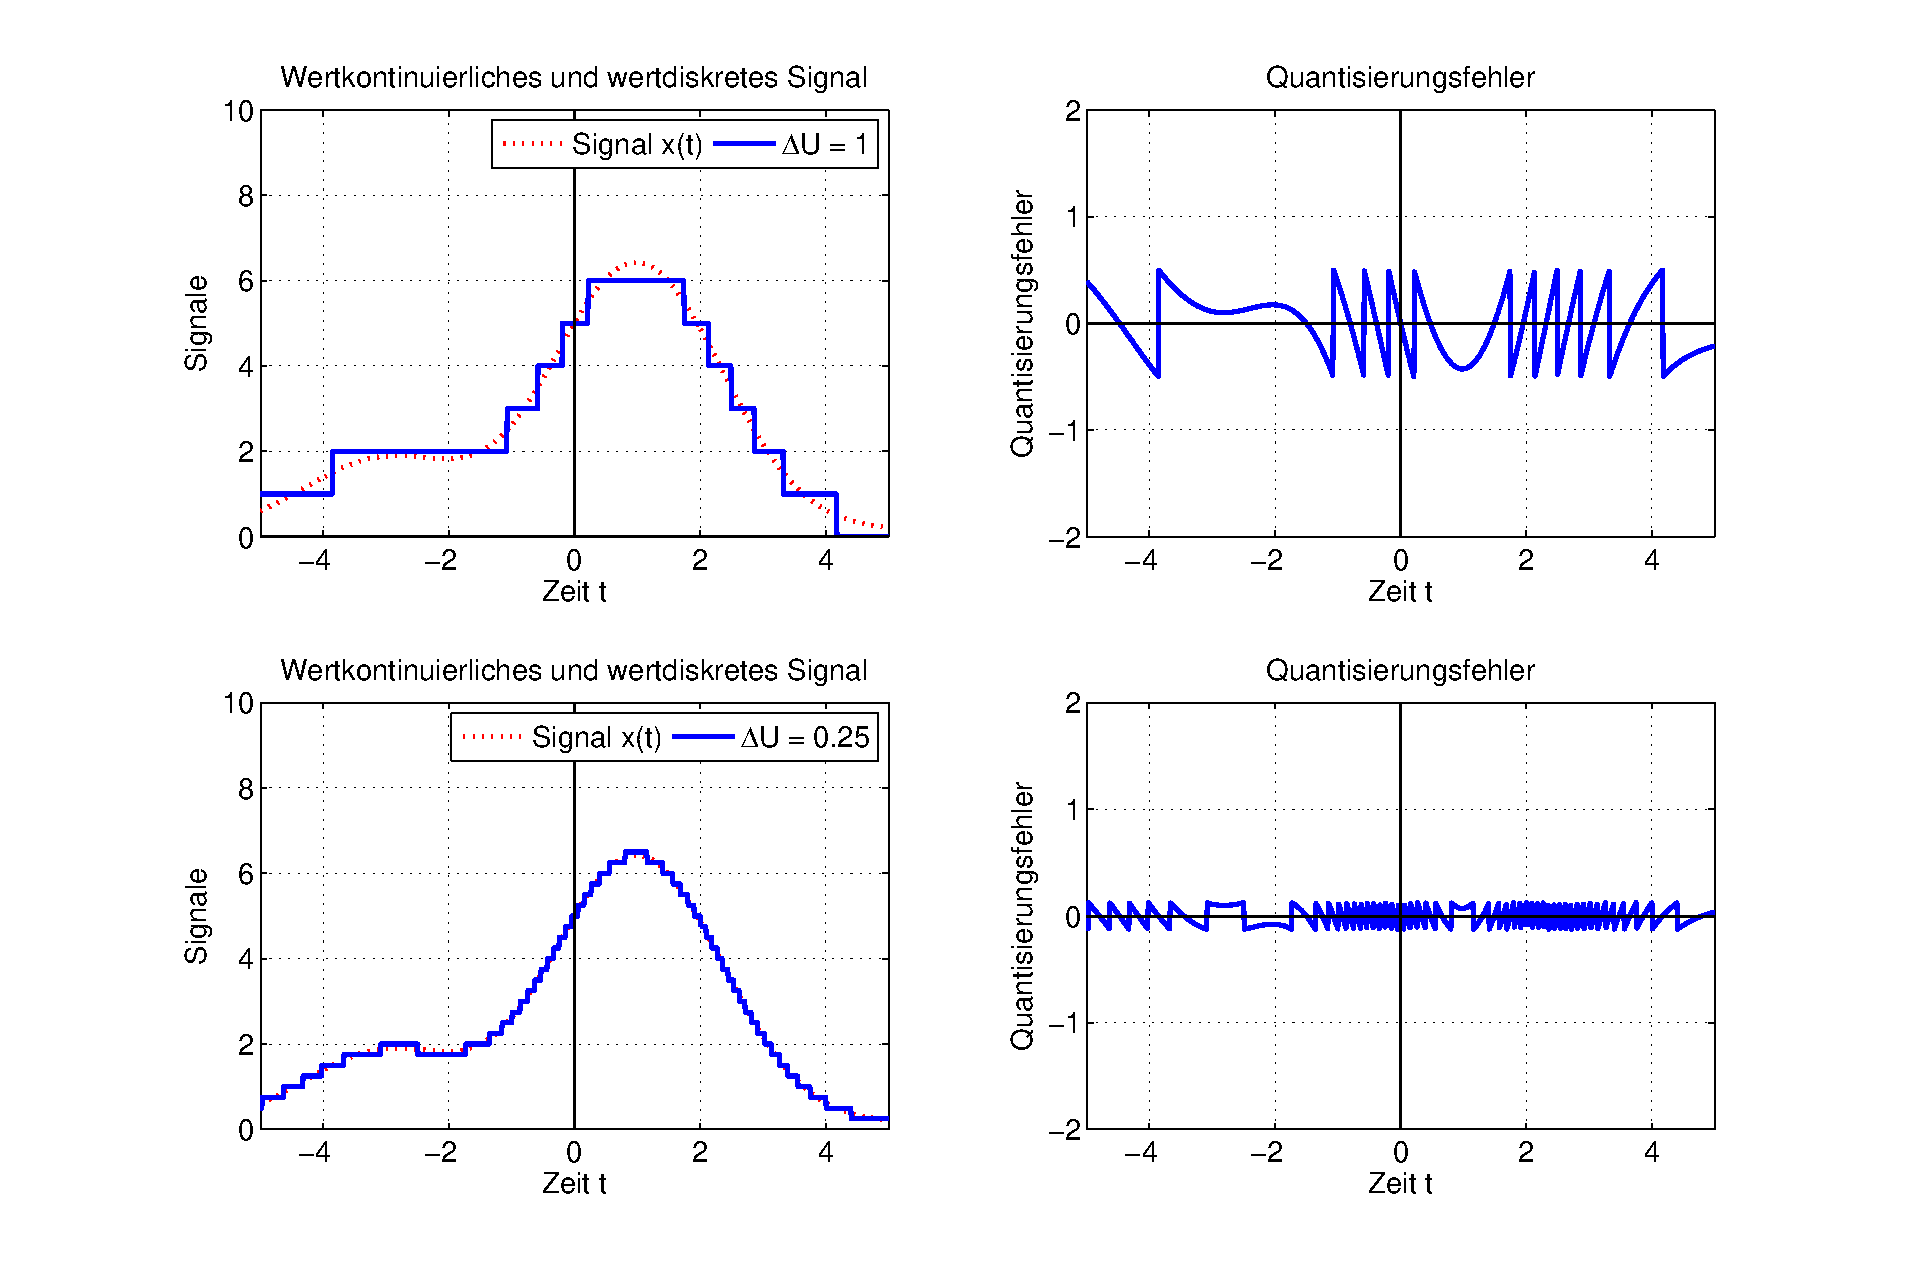
\includegraphics[width=1\textwidth]{Kapitel1/Bilder/image1}}
  \caption{Darstellung des Quantisierungsfehlers (Quantisierungsrauschens)}
  \label{fig:Quantisierungsfehler}
\end{figure}

\noindent Der Quantisierungsfehler ergibt sich aus der Differenz zwischen dem wertkontinuierlichen und dem wertdiskreten Signal. Je feiner die Auflösung des AD-Wandlers ist, desto geringer ist der Abstand zwischen dem kontinuierlichen und dem quantisierten Signal. Da die Abweichung einen zufälligen Verlauf zu haben scheint, wird dieser Fehler als Quantisierungsrauschen bezeichnet und als zufälliger Fehler oder zufälliges Störsignal behandelt. Der Umgang mit zufälligen Signalen ist Gegenstand des Teils C dieser Buchreihe, der Quantisierungsfehler wird an dieser Stelle deshalb nicht weiter vertieft.

\clearpage


\subsection{Vorüberlegungen zur zeitlichen Diskretisierung}

\noindent Die grundlegende Frage bei der zeitlichen Abtastung von Signalen ist, in welchen Zeitabständen T$_{A}$ beziehungsweise mit welcher Abtastfrequenz f$_{A}$ ein Signal erfasst werden muss. Die Bedeutung dieser Frage wird an einem Beispiel erläutert. \bigskip

\noindent
\colorbox{lightgray}{%
\arrayrulecolor{white}%
\renewcommand\arraystretch{0.6}%
\begin{tabular}{ wl{16.5cm} }
{\fontfamily{phv}\selectfont{Beispiel: Abtastwerte} }
\end{tabular}%
}\bigskip

\noindent Bild \ref{fig:AbtastwerteUnterschiedlicheAbtastzeiten} zeigt Abtastwerte eines Signals, das mit unterschiedlichen Abtastzeiten T$_{A}$ abgetastet wird. Die Abtastwerte sind jeweils über Geradenabschnitte miteinander verbunden. Das Signal scheint davon abzuhängen, wie es abgetastet wird.

\begin{figure}[H]
  \centerline{\includegraphics[width=0.5\textwidth]{Kapitel1/Bilder/image2}}
  \caption{Darstellung der Abtastwerte eines Signals, das mit unterschiedlichen Abtastzeiten T$_{A}$ abgetastet wird}
  \label{fig:AbtastwerteUnterschiedlicheAbtastzeiten}
\end{figure}


\noindent Das zugrunde liegende Signal ist sinusförmig und wird mit der Funktion

\begin{equation}\label{eq:twotwo}
u\left(t\right)=1{\rm \; }V\cdot \sin \left(2\cdot \pi \cdot 6\cdot t\right)
\end{equation}

\noindent beschrieben. D Der Vergleich der Abtastwerte mit dem Signal u(t) in Bild 2.3zeigt, dass alle in Bild 2.2 dargestellten abgetasteten Signale falsch oder zumindest irreführend sind.

\begin{figure}[H]
  \centerline{\includegraphics[width=0.5\textwidth]{Kapitel1/Bilder/image2}}
  \caption{Vergleich der Abtastwerte eines harmonischen Signals mit dem Originalsignal}
  \label{fig:Vergleich}
\end{figure}

\noindent Die Abtastwerte liegen auf einer Schwingung mit wesentlich höherer Frequenz und geben nicht das eigentliche Signal wieder. Daraus kann die Schlussfolgerung gezogen werden, dass beim Abtasten Regeln eingehalten werden müssen, um das Signal richtig rekonstruieren zu können. Diese Überlegung wird zu dem Abtasttheorem führen. 

\clearpage

\noindent Vor der allgemeinen Herleitung des Abtasttheorems werden die Abtastwerte eines harmonischen Signals x(t) mit einer Frequenz f$_{0}$ analysiert. Das Signal ist definiert als 

\begin{equation}\label{eq:twothree}
x\left(t\right)=\sin \left(2\cdot \pi \cdot f_{0} \cdot t\right)
\end{equation}

\noindent Das Signal wird mit einer Abtastzeit T${}_{A}$ abgetastet, sodass sich an den ganzzahligen Vielfachen k der Abtastzeit t~=~k$\cdot$T${}_{A}$ die Werte ergeben zu

\begin{equation}\label{eq:twofour}
x\left[k\right]=x\left(k\cdot T_{A} \right)=\sin \left(2\cdot \pi \cdot f_{0} \cdot k\cdot T_{A} \right)
\end{equation}

\noindent Die Abtastwerte der Signalfolge stimmen mit einer Signalfolge überein, die sich aus der Abtastung eines harmonischen Signals mit einer Frequenz f${}_{0}$ und dem Vielfachen der Abtastfrequenz n$\cdot$f${}_{A}$ ergibt. Einsetzen der Bedingungen ergibt 

\begin{equation}\label{eq:twofive}
\begin{split}
\sin \left(2\cdot \pi \cdot \left(f_{0} +n\cdot f_{A} \right)\cdot k\cdot T_{A} \right) 
& = \sin \left(2\cdot \pi \cdot \left(f_{0} \cdot k\cdot T_{A} +\frac{n}{T_{A} } \cdot k\cdot T_{A} \right)\right) \\ 
& = \sin \left(2\cdot \pi \cdot f_{0} \cdot k\cdot T_{A} +2\cdot \pi \cdot n\cdot k\right)=\sin \left(2\cdot \pi \cdot f_{0} \cdot k\cdot T_{A} \right)  
\end{split}
\end{equation}

\noindent Der Faktor n$\cdot$k ist dabei ein ganzzahliger Wert. Das bedeutet, dass die Abtastwerte, die ein Signal der Frequenz f${}_{0}$ repräsentieren, genau dieselben sind wie diejenigen, die sich beim Abtasten eines Signals der Frequenz f${}_{0}$ und einem Vielfachen der Abtastfrequenz f${}_{A}$ ergeben. Nach der Abtastung kann also nicht zwischen Signalen der Frequenz f${}_{0}$ und f$_{0}$ + n $\cdot$f$_{A}$ unterschieden werden. Bild \ref{fig:AbtastwerteHarmonischesSignal} stellt die Signal- und Abtastwerte für ein Beispiel dar.

\begin{figure}[H]
  \centerline{\includegraphics[width=1\textwidth]{Kapitel1/Bilder/image4}}
  \caption{Abtastwerte für ein harmonisches Signal mit der Frequenz f${}_{01}$ = 1 kHz und f${}_{02}$ = 11 kHz}
  \label{fig:AbtastwerteHarmonischesSignal}
\end{figure}

\noindent Das Signal wird mit einer Frequenz f${}_{A}$ = 10 kHz abgetastet. Die Abtastwerte sind für ein Signal mit einer Frequenz f${}_{1}$~=~1~kHz und einem Signal mit einer Frequenz f${}_{2}$ = 11 kHz identisch.\newline

\noindent Der hier für harmonische Schwingungen dargestellte Sachverhalt gilt auch für nicht harmonische Signale, da sie sich mit der Fourier-Transformation auf harmonische Signale zurückführen lassen. Dieser Effekt macht es erforderlich, den Abtastvorgang mathematisch zu beschreiben und Bedingungen für den Abtastvorgang zu definieren, unter denen ein abgetastetes Signal rekonstruiert werden kann.

\clearpage


\subsection{Ideale Abtastung und ideale Rekonstruktion}

\noindent Für die systemtheoretische Behandlung der digitalen Signalverarbeitung ist es erforderlich, die Abtastung und die Rekonstruktion des Signals mathematisch ideal zu beschreiben. Aus dieser Beschreibung wird anschlie{\ss}end das Abtasttheorem hergeleitet.


\subsubsection{Mathematische Beschreibung der idealen Abtastung}

\noindent Um die Abtastung eines Signals mathematisch beschreiben zu können, wird eine sogenannte Abtastfunktion a(t) definiert. Da bei der idealen Abtastung Werte des analogen Signals zu diskreten Zeitpunkten erfasst werden, bietet sich eine Folge von Impulsen als Abtastfunktion an. Diese Abtastfunktion a(t) ist mathematisch definiert als 

\begin{equation}\label{eq:twosix}
a\left(t\right)=\sum _{k=-\infty }^{\infty }\delta \left(t-k\cdot T_{A} \right) 
\end{equation}

\noindent Die Abtastfunktion wird mit dem analogen Signal x(t) multipliziert. Da die Impulsfolge nur zu den Zeitpunkten k$\cdot$T$_{A}$ ungleich null ist, genügt es, die Funktion x(t) nur zu diesen Zeitpunkten zu betrachten. Es ergibt sich als Darstellung für das ideal abgetastete Signal x$_{A}$(t)

\begin{equation}\label{eq:twoseven}
x_{A} \left(t\right)=x\left(t\right)\cdot a\left(t\right)=x\left(t\right)\cdot \sum _{k=-\infty }^{\infty }\delta \left(t-k\cdot T_{A} \right) =\sum _{k=-\infty }^{\infty }x\left(k\cdot T_{A} \right)\cdot \delta \left(t-k\cdot T_{A} \right)
\end{equation}

\noindent Bild \ref{fig:AbtastprozessIdealSignal} verdeutlicht die mathematische Beschreibung der Signale grafisch. Dabei werden die unendlich gro{\ss}en Impulse als Pfeile dargestellt, ihre Höhe repräsentiert das Gewicht des jeweiligen Impulses.

\begin{figure}[H]
  \centerline{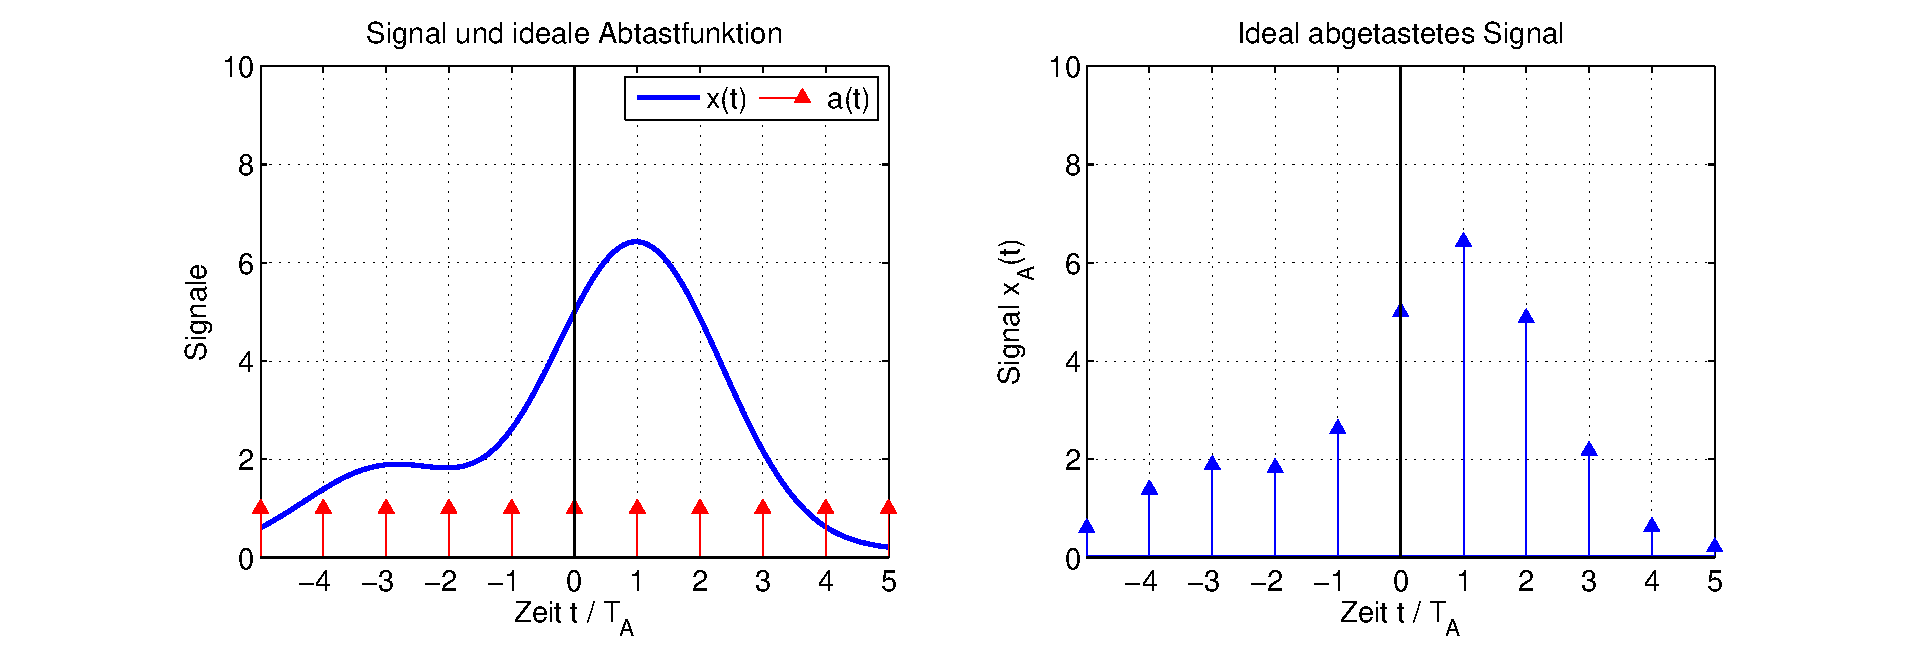
\includegraphics[width=1\textwidth]{Kapitel1/Bilder/image5}}
  \caption{Darstellung der Signale im idealen Abtastprozess
}
  \label{fig:AbtastprozessIdealSignal}
\end{figure}

\noindent Wird dieser Vorgang im Frequenzbereich betrachtet, wird deutlich, dass durch das Abtasten das Spektrum des Signals periodisch wird. Im Zeitbereich wird das Signal x(t) mit der Abtastfunktion a(t) multipliziert. Der Multiplikation im Zeitbereich entspricht eine Faltung im Frequenzbereich. Damit muss im Frequenzbereich das Spektrum des Signals X($\omegaup$) mit dem Spektrum der Abtastfunktion A($\omegaup$) gefaltet werden. Hierfür wird zunächst das Spektrum der Abtastfunktion errechnet.

\begin{equation}\label{eq:twoeight}
\Im \left\{a\left(t\right)\right\}=\Im \left\{\sum _{k=-\infty }^{\infty }\delta \left(t-k\cdot T_{A} \right) \right\}
\end{equation}

\noindent Die Gleichung kann als Fourier-Reihe dargestellt werden und in den folgenden Ausdruck umgeformt werden

\begin{equation}\label{eq:twonine}
\Im \left\{a\left(t\right)\right\}=\Im \left\{\sum _{k=-\infty }^{\infty }\delta \left(t-k\cdot T_{A} \right) \right\}=\frac{2\cdot \pi }{T_{A} } \cdot \sum _{k=-\infty }^{\infty }\delta \left(\omega -k\cdot \frac{2\cdot \pi }{T_{A} } \right) =\frac{2\cdot \pi }{T_{A} } \cdot \sum _{k=-\infty }^{\infty }\delta \left(\omega -k\cdot \omega _{A} \right) 
\end{equation}

\noindent Dies bedeutet, dass die Abtastfunktion auch im Frequenzbereich einer Impulsfolge entspricht, wobei der Abstand der Impulse proportional zur Abtastfrequenz

\begin{equation}\label{eq:twoten}
\omega _{A} =2\cdot \pi \cdot f_{A} =\frac{2\cdot \pi }{T_{A} }
\end{equation}

\noindent ist. Über die Faltungsbeziehung ergibt sich für die abgetastete Funktion x$_{A}$(t) im Frequenzbereich 

\begin{equation}\label{eq:twoeleven}
\begin{split}
X_{A} \left(\omega \right) & = \frac{1}{2\cdot \pi } \cdot \left(X\left(\omega \right)*\left(\frac{2\cdot \pi }{T_{A} } \cdot \sum _{k=-\infty }^{\infty }\delta \left(\omega -k\cdot \frac{2\cdot \pi }{T_{A} } \right) \right)\right) \\ 
& = \frac{1}{T_{A} } \cdot \sum _{k=-\infty }^{\infty }X\left(\omega -k\cdot \frac{2\cdot \pi }{T_{A} } \right) =\frac{1}{T_{A} } \cdot \sum _{k=-\infty }^{\infty }X\left(\omega -k\cdot \omega _{A} \right)    
\end{split}
\end{equation}

\noindent Die Eine Abtastung mit einer idealen Impulsreihe der idealen Abtastfunktion führt demnach zu einer in $\omega{A}$ periodischen Fortsetzung des Spektrums X($\omega$) des kontinuierlichen Zeitsignals x(t) und zu einer Multiplikation mit dem Faktor 1/T${}_{A}$. Bild \ref{fig:AbtastprozessIdealSpektrum} stellt die Spektren im idealen Abtastprozess schematisch dar.

\begin{figure}[H]
  \centerline{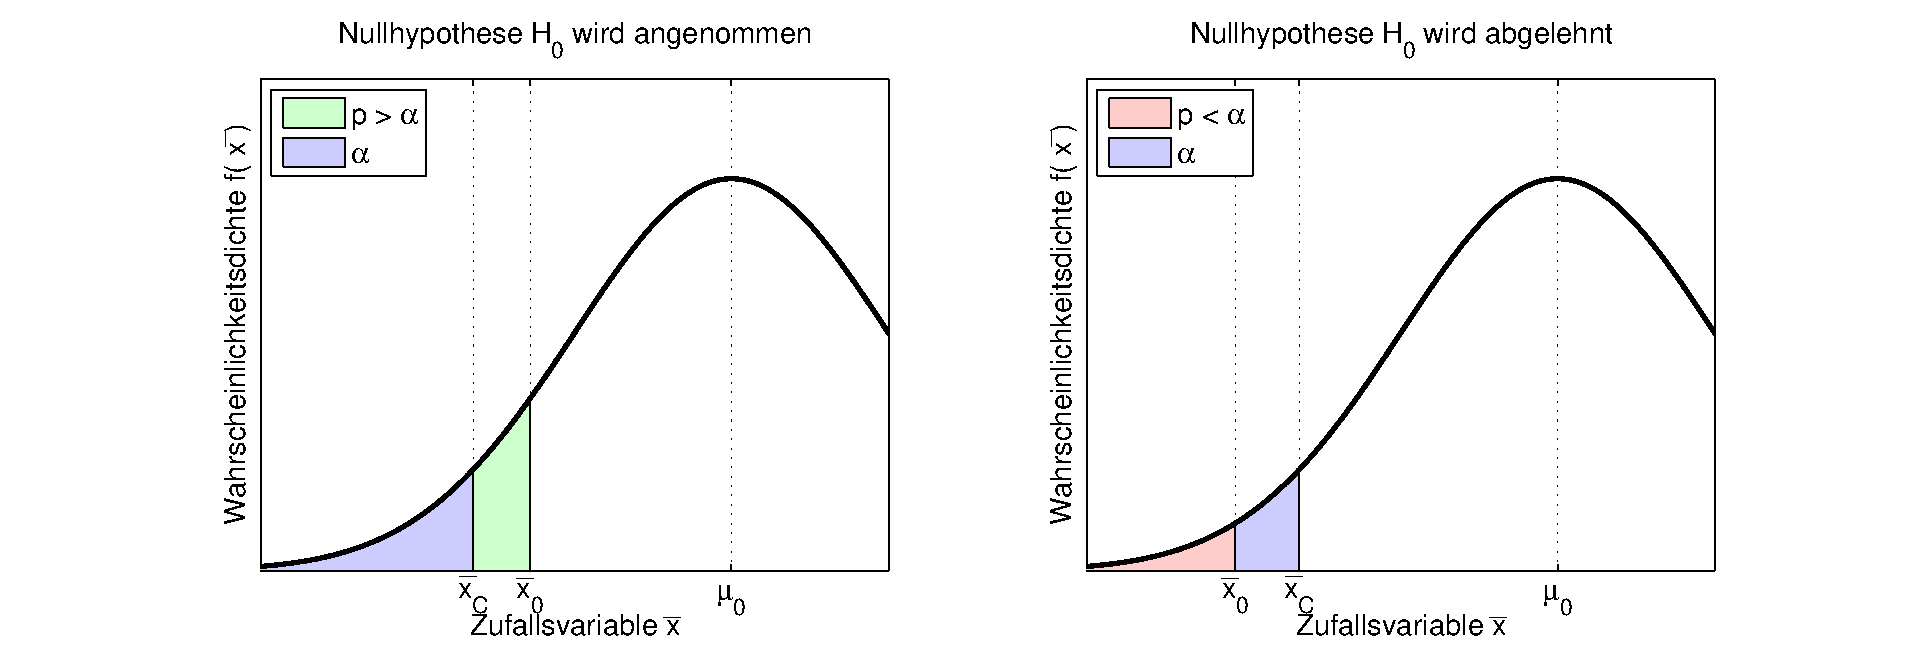
\includegraphics[width=1\textwidth]{Kapitel1/Bilder/image6}}
  \caption{Darstellung der Spektren im idealen Abtastprozess}
  \label{fig:AbtastprozessIdealSpektrum}
\end{figure}

\noindent Die periodische Wiederholung des Spektrums ist dafür verantwortlich, dass die Abtastwerte von zu langsam abgetasteten Signalen mit den Frequenzen f${}_{0}$ und f${}_{0}$ + n$.$f${}_{A}$ nicht unterschieden werden können. Die mathematische Herleitung bestätigt damit den in Bild \ref{fig:AbtastprozessIdealSpektrum} dargestellten Sachverhalt.

\noindent Der ursprüngliche Frequenzbereich des Signals x(t) mit dem Frequenzbereich - $\omega_{G}$ $\leq$ $\omega$ $\leq$ $\omega_{G}$ wird als Basisband des Signals bezeichnet. Durch den Abtastvorgang wird das Basisband periodisch in $\omega_{A}$ wiederholt.


\subsubsection{Ideale Rekonstruktion eines Signals}

\noindent Da bei der idealen Abtastung das Spektrum eines Signals periodisch wiederholt und mit dem Faktor 1/T${}_{A}$ multipliziert wird, liegt es auf der Hand, die Wiederholung des Spektrums durch eine entsprechende Filterung zu eliminieren. Durch eine hier ideal angenommene Tiefpass-Funktion mit einer Bandbreite Grenzfrequenz von $\omega_{A}$/2 kann das sogenannte Basisband, also das ursprüngliche Spektrum der Zeitfunktion, isoliert werden. Bild \ref{fig:RekonstruktionIdeal} verdeutlicht den Filterprozess.

\begin{figure}[H]
  \centerline{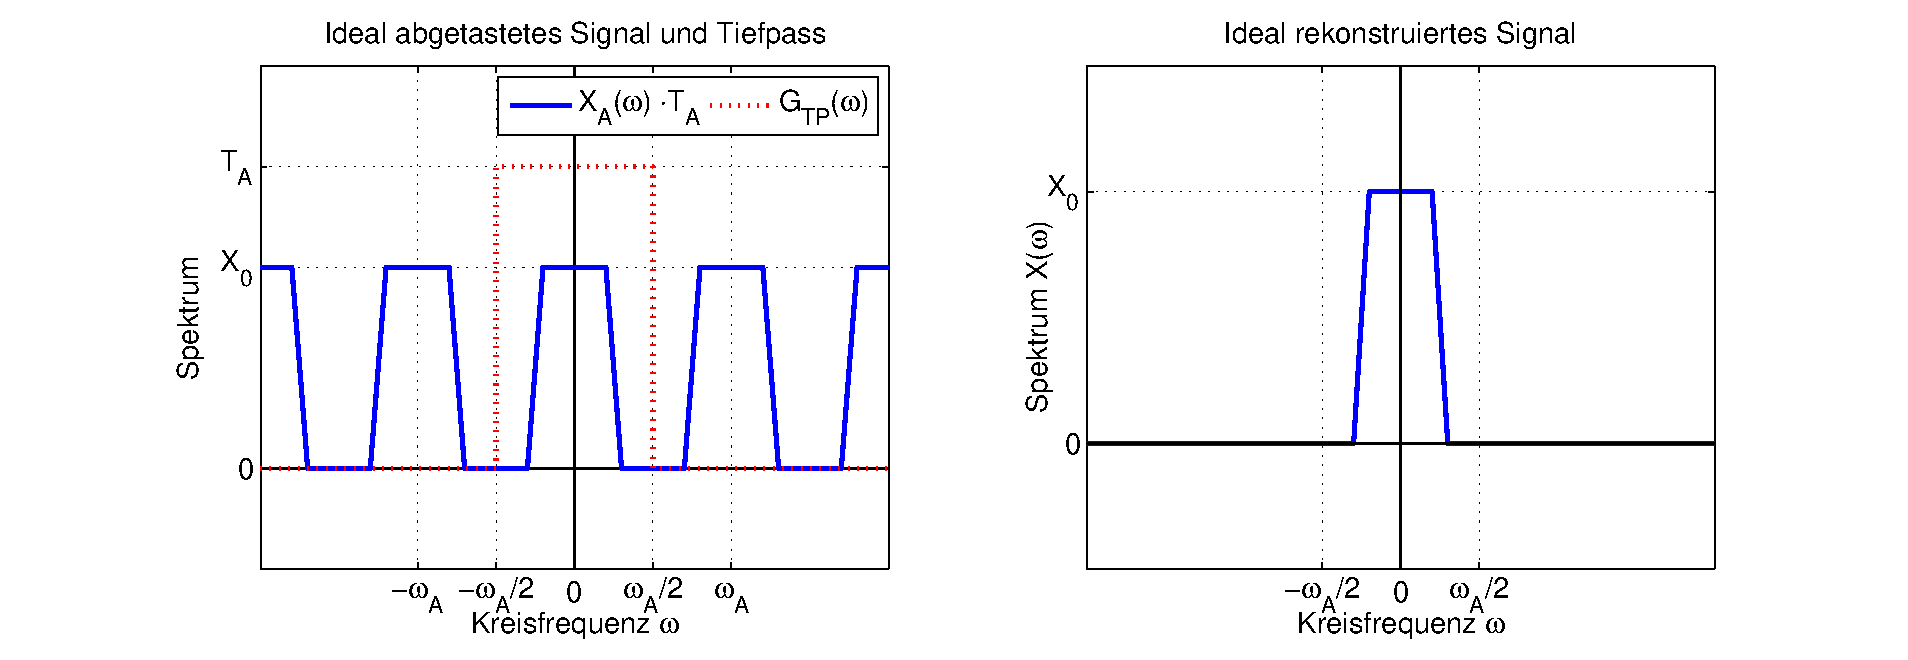
\includegraphics[width=1\textwidth]{Kapitel1/Bilder/image7}}
  \caption{Rekonstruktion des Spektrums der Zeitfunktion durch ideale Tiefpass-Filterung, idealisierte Tiefpass-Funktion gestrichelt dargestellt}
  \label{fig:RekonstruktionIdeal}
\end{figure}

\noindent Mathematisch gesehen muss das Spektrum mit einer idealen Tiefpass-Filterfunktion und dem Faktor T${}_{A}$ multipliziert werden. Das Spektrum ergibt sich damit zu

\begin{equation}\label{eq:twotwelve}
\begin{split}
X\left(\omega \right) & = G_{TP} \left(\omega \right)\cdot X_{A} \left(\omega \right)=T_{A} \cdot \left(\sigma \left(\omega +\frac{\omega _{A} }{2} \right)-\sigma \left(\omega -\frac{\omega _{A} }{2} \right)\right)\cdot \frac{1}{T_{A} } \cdot \sum _{k=-\infty }^{\infty }X\left(\omega -k\cdot \omega _{A} \right)\\
& =
\end{split}
\end{equation}


\noindent Die ideale Rekonstruktion kann auch im Zeitbereich durchgeführt werden. Der Multiplikation im Frequenzbereich entspricht im Zeitbereich die Faltung der entsprechenden Zeitfunktionen. Die Impulsantwort g$_{TP}$(t) der Filterfunktion G$_{TP}$($\omega$) ist nach den Rechenregeln der Fourier-Transformation 

\begin{equation}\label{eq:twothirteen}
g_{TP} \left(t\right)=\frac{T_{A} }{\pi } \cdot \frac{\sin \left(\frac{\omega _{A} }{2} \cdot t\right)}{t}
\end{equation}

\noindent Die Funktion Impulsantwort de Tiefsses ist in Bild \ref{fig:RekonstruktionIdealSignal} dargestellt. Zum Zeitpunkt t = 0 ist die Funktion 1, zu den Zeitpunkten k$\cdot$T${}_{A}$ ist die Funktion null.

\begin{figure}[H]
  \centerline{\includegraphics[width=0.5\textwidth]{Kapitel1/Bilder/image8}}
  \caption{Impulsantwort des idealen Tiefpass-Filters zur Rekonstruktion}
  \label{fig:RekonstruktionIdealSignal}
\end{figure}

\noindent Das Signal x(t) berechnet sich über das Faltungsintegral. Da die Faltung einer Funktion x(t) mit einem Impuls an der Stelle t$_{0}$ die Funktion an die Stelle x(t - t$_{0}$) verschiebt, ergibt sich

\begin{equation}\label{eq:twofourteen}
\begin{split}
x\left(t\right) & = g_{TP} \left(t\right)*x_{A} \left(t\right)=\frac{T_{A} }{\pi } \cdot \frac{\sin \left(\frac{\omega _{A} }{2} \cdot t\right)}{t} *\sum _{k=-\infty }^{\infty }x\left(k\cdot T_{A} \right)\cdot \delta \left(t-T_{A} \cdot k\right) \\ {} 
\end{split}
\end{equation}

\noindent Das Signal setzt sich aus der Summe von Termen g$_{TP}$(t) zusammen, die jeweils um k$\cdot$T${}_{A}$ verschoben sind und mit dem Gewicht x(k$\cdot$T${}_{A}$) multipliziert werden. Bild \ref{fig:RekonstruktionIdealSignalimZeit} stellt die Rekonstruktion im Zeitbereich dar.

\begin{figure}[H]
  \centerline{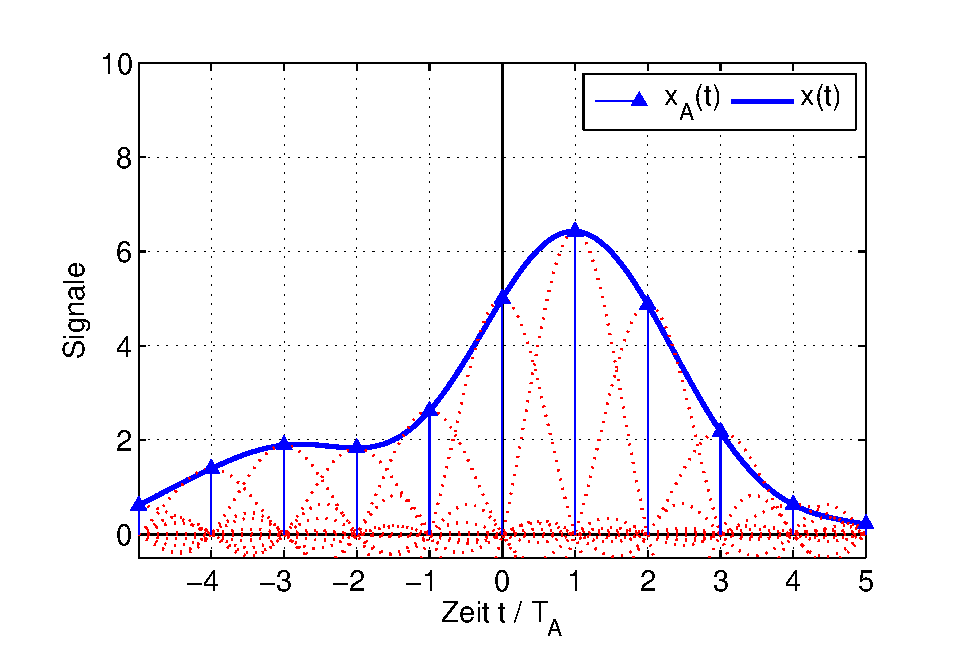
\includegraphics[width=0.5\textwidth]{Kapitel1/Bilder/image9}}
  \caption{Rekonstruktion eines ideal abgetasteten Signals im Zeitbereich}
  \label{fig:RekonstruktionIdealSignalimZeit}
\end{figure}


\noindent Das Ergebnis der Überlagerung ist enspricht erwartungsgemä{\ss} die der ursprüngliche Zeitfunktion x(t).


\subsubsection{Abtasttheorem nach Shannon}

\noindent In den vorangegangenen Abschnitten wird gezeigt, dass sich das Spektrum eines abgetasteten Signals periodisch mit der Abtastfrequenz $\omega_{A}$ fortsetzt. Diese periodische Wiederholung ist Grundlage für die Herleitung des Abtasttheorems nach Shannon.

\noindent Gegeben sei ein bandbegrenztes Signal x(t), das abgetastet werden soll. Durch die Physik des Systems ist die Bandbreite des Signals auf Frequenzen $\omega\mathrm{\le}$ $\omega_{G}$ begrenzt. Bei der Abtastung des Signals wird das Spektrum der Zeitfunktion, wie in Bild \ref{fig:RekonstruktionIdeal} dargestellt, periodisch in $\omega_{A}$ wiederholt. Durch eine hier ideal angenommene Tiefpass-Funktion kann das sogenannte Basisband, also das ursprüngliche Spektrum der Zeitfunktion, isoliert werden. Bild \ref{fig:RekonstruktionIdeal} verdeutlicht den Filterprozess.

\noindent Ist die Abtastzeit T${}_{A}$ zu gro{\ss}, wird $\omega_{A}$ zu klein und die einzelnen Spektren der abgetasteten Funktion überlagern sich. Signalverzerrungen, die sich beim Abtasten durch Überlagerung der Spektren ergeben, werden als Aliasing bezeichnet. Damit die einzelnen Spektren voneinander getrennt bleiben, muss nach Bild \ref{fig:RekonstruktionIdeal} die Bedingung 

\begin{equation}\label{eq:twofifteen}
\omega _{G} <\omega _{A} -\omega _{G}
\end{equation}

\noindent beziehungsweise 

\begin{equation}\label{eq:twosixteen}
\omega _{A} =2\cdot \pi \cdot \frac{1}{T_{A} } >2\cdot \omega _{G}
\end{equation}

\noindent erfüllt sein. Dieses Ergebnis wird als Abtasttheorem bezeichnet. Die Abtastfrequenz $\omega_{A}$ muss mindestens mehr als doppelt so gro{\ss} sein wie die Bandbreite $\omega_{G}$ des abzutastenden Signals. Damit muss für die Abtastzeit T$_{A}$ gelten: 

\begin{equation}\label{eq:twoseventeen}
T_{A} <\frac{\pi }{\omega _{G} } 
\end{equation}

\noindent Bild \ref{fig:SpektrenAbgetasteterSignale} zeigt die Spektren abgetasteter Signale für genügend gro{\ss}e Abtastfrequenz, gerade ausreichende und zu kleine Abtastfrequenz. 


\noindent Im ersten Fall X$_{A1}$($\omega$) wird mit einer Abtastfrequenz gearbeitet, die deutlich grö{\ss}er ist als das Abtasttheorem vorschreibt. Dieser Fall wird als Oversampling bezeichnet. Durch die hohe Abtastfrequenz werden das Spektrum im Basisband und die nächsthöheren Spektren deutlich voneinander getrennt, sodass mit einem Tiefpass-Filter mit vergleichsweise flachem Übergang zwischen Sperr- und Durchlass-Bereich gearbeitet werden kann.

\noindent Im zweiten Fall X${}_{A2}$($\omega$) wird das Abtasttheorem gerade eingehalten. Es zeigt sich aber, dass die Rekonstruktion nur mit einem idealen Tiefpass-Filter erfolgen kann, der technisch nicht realisiert werden kann. Dieser Fall entspricht dem theoretischen Grenzfall des Abtasttheorems. 

\noindent Im Fall einer zu kleinen Abtastfrequenz X$_{A3}$($\omega$) überlagern sich die Spektren. Das Signal kann selbst mit einem idealen Tiefpass-Filter nicht fehlerfrei rekonstruiert werden. Es kommt zu Signalverzerrungen oder Aliasing. 
\begin{figure}[H]
  \centerline{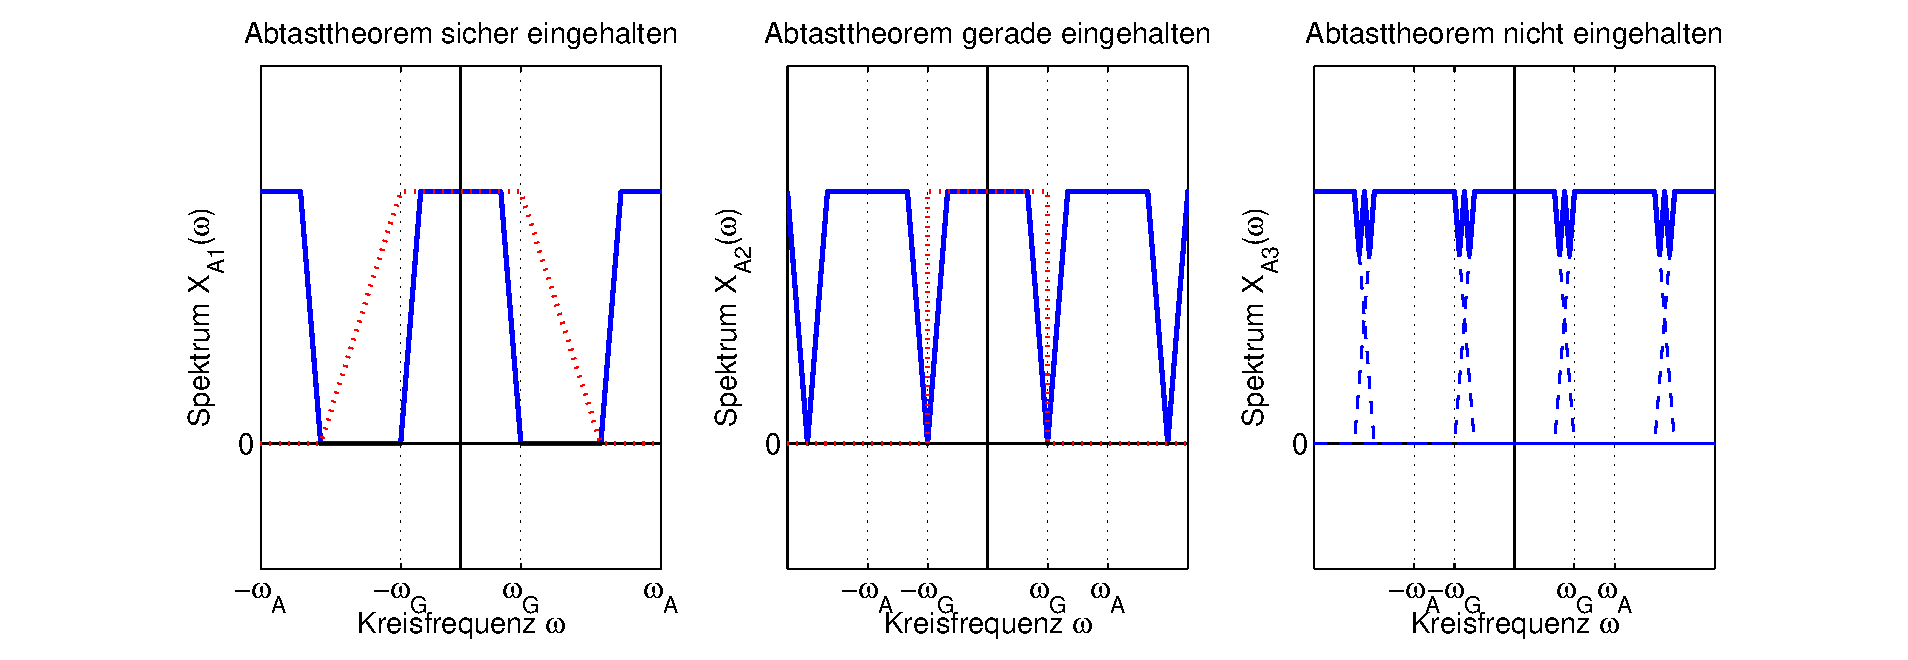
\includegraphics[width=1\textwidth]{Kapitel1/Bilder/image10}}
  \caption{Spektren abgetasteter Signale für genügend gro{\ss}e Abtastfrequenz X$_{A1}$($\omega$), gerade ausreichende Abtastfrequenz X$_{A2}$($\omega$) und für zu kleine Abtastfrequenz X$_{A3}$($\omega$)}
  \label{fig:SpektrenAbgetasteterSignale}
\end{figure}

\noindent
\colorbox{lightgray}{%
\arrayrulecolor{white}%
\renewcommand\arraystretch{0.6}%
\begin{tabular}{ wl{16.5cm} }
{\fontfamily{phv}\selectfont{Beispiel: Abtastrate einer Sound-Karte} }
\end{tabular}%
}\medskip

\noindent Sound-Karten von Computern besitzen einen Analog-Digital-Wandler (ADC). Er wandelt das analoge Signal in ein digitales Signal um. Bei Sound-Karten ist zum einen die Auflösung des ADC wichtig, da sie die Quantisierungsfehler und damit das Rauschen bestimmt. Zweiter wesentlicher Faktor ist die Abtastrate.

\begin{figure}[H]
  \centerline{\includegraphics[width=0.5\textwidth]{Kapitel1/Bilder/image11}}
  \caption{Sound-Karte für Personal Computer}
  \label{fig:SoundKarte}
\end{figure}

\noindent Eine Abtastfrequenz f$_{A}$ = 44 kHz ermöglicht die Aufnahme und Wiedergabe bis zu einer theoretischen Bandbreite von 

\begin{equation}\label{eq:twoeighteen}
f_{G} =\frac{f_{A} }{2} =22{\rm \; }kHz
\end{equation}

\noindent Mit der Sound-Karte können damit Musiksignale mit einer maximalen Frequenz von 22 kHz verarbeitet werden.


\subsubsection{Bandbegrenzung des abzutastenden Signals}

\noindent Das Abtasttheorem geht davon aus, dass das Signal bandbegrenzt ist. Reale Signale haben in praktischen Anwendungen aber im Allgemeinen keine harte Bandbegrenzung. Vielmehr ergibt sich ihre Bandbreite aus dem Tiefpassverhalten des Systems, das das Signal generiert, und dem Spektrum von überlagerten Störungen. Um den Einfluss der mangelhaften Bandbegrenzung zu reduzieren, kann ein analoger Tiefpass wie zum Beispiel ein RC-Glied zur Filterung eingesetzt werden. Er verhindert, dass sich in dem Spektrum höhere Frequenzanteile befinden als erwartet, und reduziert damit den Einfluss von Störungen. Das Tiefpass-Filter wird aufgrund seiner Funktion als Anti-Aliasing-Filter bezeichnet. Die Wirkung des Anti-Aliasing-Filters wird in Bild \ref{fig:AntiAliasingFilterWirkung} veranschaulicht.

\begin{figure}[H]
  \centerline{\includegraphics[width=1\textwidth]{Kapitel1/Bilder/image12}}
  \caption{Wirkung des Anti-Aliasing-Filters auf die Bandbegrenzung des Spektrums X($\omega$) des Signals x(t)}
  \label{fig:AntiAliasingFilterWirkung}
\end{figure}

\noindent Das Signal x(t) hat ein Spektrum, dessen Information im Nutzbereich - $\omega_{N} \; \mathrm{<} \; \omega \;  \mathrm{<} \; \omega_{N}$ liegt. Es besitzt aber zum Beispiel aufgrund von Störungen ein breiteres Spektrum. Damit existieren auch oberhalb der als maximal angenommenen Bandbreite $\omega _{G}$ Spektralanteile. Durch den Einsatz eines Tiefpass-Filters, das den Frequenzbereich $\omega \; \mathrm{<}$ - $\omega_{N}$ und den Bereich $\omega \; \mathrm{>} \; \omega_{N}$ dämpft, ergibt sich bei dem neu entstandenen Signal ein Spektrum X$_{TP}$ ($\omega$), das im Nutzbereich dem des ursprünglichen Signals entspricht, im übrigen Bereich aber stärker gedämpft ist. Dieses Signal kann wegen der geringeren Bandbreite $\omega_{GTP} \;  \mathrm{<} \;  \omega_{G}$ mit einer geringeren Frequenz abgetastet werden und der Rauschanteil wird durch die Bandbegrenzung reduziert.

\noindent In technischen Anwendungen wird deshalb praktisch immer ein Eingangstiefpass eingesetzt, das das Spektrum des Eingangssignals auf die notwendige Bandbreite begrenzt. Die Spezifikation von Filtern und ihr Entwurf werden im Teil A dieser Buchreihe diskutiert.\bigskip

\noindent
\colorbox{lightgray}{%
\arrayrulecolor{white}%
\renewcommand\arraystretch{0.6}%
\begin{tabular}{ wl{16.5cm} }
{\fontfamily{phv}\selectfont{Beispiel: Abtastung Drucksensor im Steuergerät} }
\end{tabular}%
}\medskip

\noindent Für die Regelung des Ladedrucks von Turboladern werden Drucksensoren eingesetzt. 

\begin{figure}[H]
  \centerline{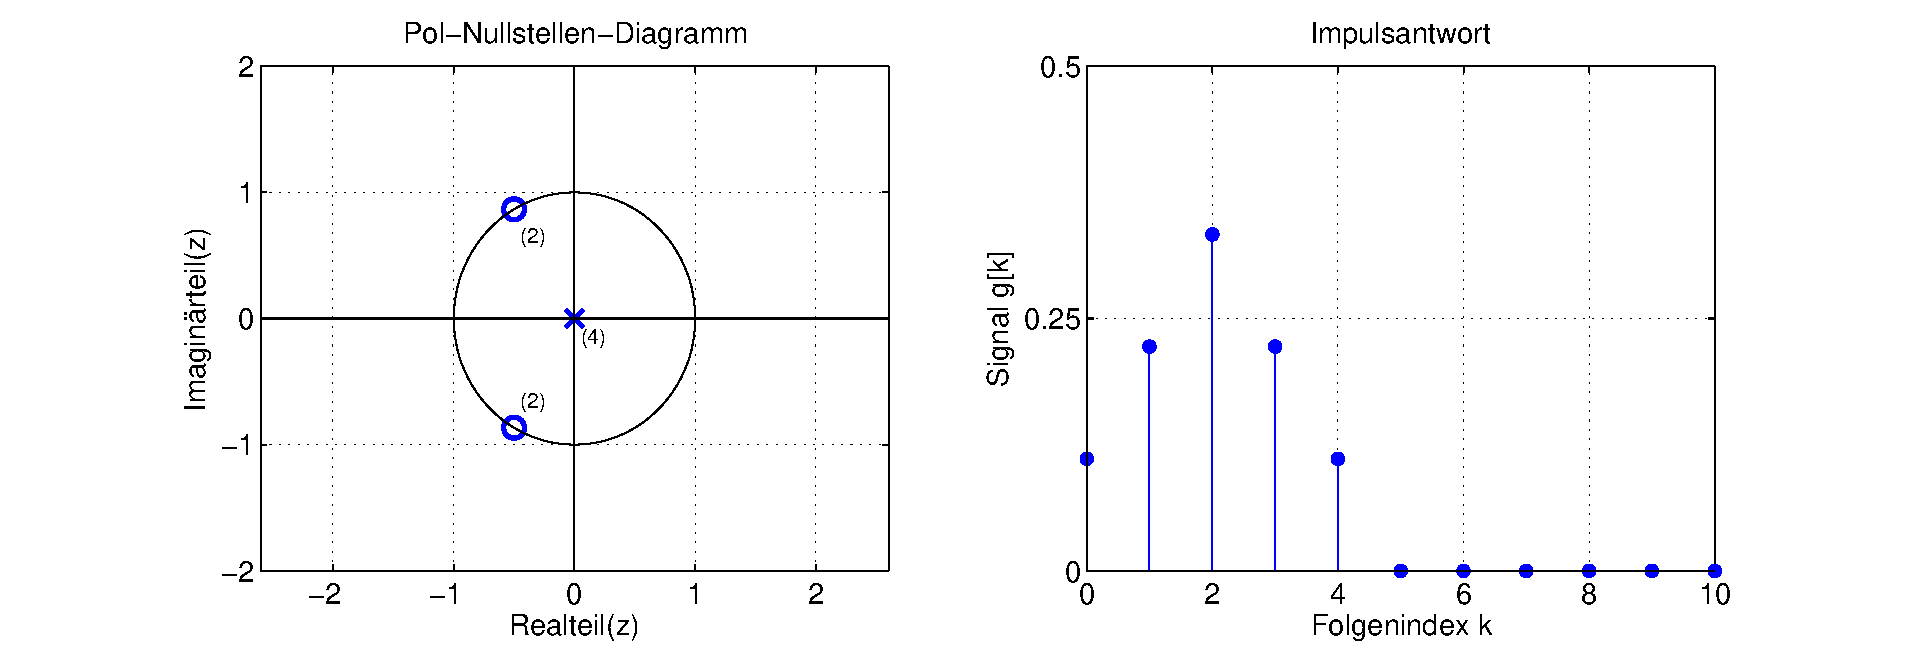
\includegraphics[width=0.3\textwidth]{Kapitel1/Bilder/image13}}
  \caption{Drucksensor zur Messung des Ladedrucks (Bosch)}
  \label{fig:Drucksensor}
\end{figure}

\noindent Der Drucksensor, der den Ladedruck misst, hat besitzt laut Datenblatt eine Zeitkonstante T = 0.1 ms. Das entspricht einer 3dB-Grenzfrequenz von 

\begin{equation}\label{eq:twonineteen}
\omega _{G} =\frac{1}{T} =10{\rm \; }krad/s
\end{equation}

\noindent Das Motor-Steuergerät tastet das Signal mit einer Abtastzeit T${}_{A}$ von 1 ms ab. Es ergibt sich eine Abtastfrequenz von 

\begin{equation}\label{eq:twotwenty}
\omega _{A} =\frac{2\cdot \pi }{T_{A} } =6.283{\rm \; k}rad/s
\end{equation}

\noindent Das Abtasttheorem ist demnach nicht erfällt. Au{\ss}erdem sind dem Sensorsignal Störungen überlagert, die Spektralanteile weit oberhalb der Grenzfrequenz besitzen können. Zur Vermeidung von Aliasing-Effekten wird ein Anti-Aliasing-Filter eingesetzt. Es weist eine Zeitkonstante von T$_{TP}$ = 0.6 ms auf, was einer 3dB-Grenzfrequenz von 

\begin{equation}\label{eq:twotwentyone}
\omega _{TP} =\frac{1}{0.6{\rm \; }ms} ={\rm 1.67\; }krad/s<3.14{\rm \; }krad/s=\frac{\omega _{A} }{2}
\end{equation}

\noindent entspricht. Durch den Einsatz des Tiefpass-Filters wird bei derselben Abtastrate das Abtasttheorem eingehalten. Das Filter hat eine Dämpfung von - 20 dB pro Dekade. Die sich aus der endlichen Steilheit ergebenden Effekte werden in einer Übungsaufgabe diskutiert.

\clearpage


\subsection{Reale Abtastung und Rekonstruktion}

\noindent Die zuvor vorgestellte ideale Abtastfunktion a(t) ist nicht realisierbar, da ideale Impulse technisch nicht erzeugt werden können. Dies liegt an der unendlich kurzen Dauer sowie der unendlichen Steilheit und Höhe von Impulsen. Aus dieser Überlegung ergeben sich die reale Abtastung und die reale Rekonstruktion von Signalen.


\subsubsection{Reale Abtastung eines Signals}

\noindent Reale beziehungsweise technisch realisierbare Abtastsysteme brauchen eine Wandlungszeit T$_{W}$, um aus dem analogen Signal ein zeitdiskretes Signal zu generieren. Die Wandlungszeit ergibt sich zum Beispiel aus einem Ladungstransport oder einem Approximationsprozess, bei dem das Signal als Mittelwert über einen Zeitraum T$_{W}$ durch Integration bestimmt wird. Das real abgetastete Signal x$_{AW}$(t) wird deshalb mit dem Ausdruck

\begin{equation}\label{eq:twotwentytwo}
x_{AW} \left(t\right)=\frac{1}{T_{W} } \cdot \int _{t-T_{W} }^{t}x\left(\tau \right)\, \, d\tau  \cdot \sum _{k=-\infty }^{\infty }\delta \left(t-k\cdot T_{A} \right) =x_{M} \left(t\right)\cdot \sum _{k=-\infty }^{\infty }\delta \left(t-k\cdot T_{A} \right)
\end{equation}

\noindent beschrieben. Es handelt sich um das Produkt von dem gleitenden Mittelwert x${}_{M}$(t) und der idealen Abtastfunktion a(t) im Zeitbereich. Zur Berechnung des Spektrums X${}_{AW}$($\omega$) müssen die Spektren der beiden Signale berechnet werden. Dazu wird das Integral in zwei Summanden zerlegt. 
\begin{equation}\label{eq:twotwentythree}
x_{M} \left(t\right)=\frac{1}{T_{W} } \cdot \int _{t-T_{W} }^{t}x\left(\tau \right)\, \, d\tau  =\frac{1}{T_{W} } \cdot \left(\int _{-\infty }^{t}x\left(\tau \right)\, \, d\tau  -\int _{-\infty }^{t-T_{W} }x\left(t\right)\, \, dt \right)
\end{equation}

\noindent Mit der Integrations- und Verschiebungsregel ergibt sich das zugehörige Spektrum.

\begin{equation}\label{eq:twotwentyfour}
\begin{split}
X_{M} \left(\omega \right) & = \frac{1}{T_{W} } \cdot \left(\frac{1}{j\cdot \omega } \cdot X\left(\omega \right)+\pi \cdot X\left(0\right)\cdot \delta \left(\omega \right)\right)\cdot \left(1-e^{-j\cdot \omega \cdot T_{W} } \right) \\ 
& = \frac{1}{T_{W} } \cdot \left(\frac{1}{j\cdot \omega } \cdot X\left(\omega \right)+\pi \cdot X\left(0\right)\cdot \delta \left(\omega \right)\right)\cdot 2\cdot j\cdot \sin \left(\frac{\omega \cdot T_{W} }{2} \right)\cdot e^{-\frac{j\cdot \omega \cdot T_{W} }{2} }  \\
& \frac{2}{\omega \cdot T_{w} } \cdot\sin \left(\frac{\omega \cdot T_{w}}{2}\right) \cdot X(\omega)\cdot e^{-\frac{j\cdot \omega \cdot T_{W} }{2} } + \frac{\pi\cdot X(0)}{T_{W}}\cdot \delta(\omega) \cdot 2 \cdot j \cdot \sin \left(\frac{\omega \cdot T_{w}}{2}\right)\cdot e^{-\frac{j\cdot \omega \cdot T_{W} }{2} }
\end{split}
\end{equation}

\noindent Da der letzte Summand in Gleichung \eqref{eq:twotwentyfour} null ist, gilt:

\begin{equation}\label{eq:twotwentyfive}
X_{M} \left(\omega \right)=\frac{2}{\omega \cdot T_{W} } \cdot \sin \left(\frac{\omega \cdot T_{W} }{2} \right)\cdot X\left(\omega \right)\cdot e^{-\frac{j\cdot \omega \cdot T_{W} }{2} }
\end{equation}

\noindent Mit dem Spektrum der idealen Abtastfunktion a(t) aus Gleichung \eqref{eq:twonine} und der Multiplikationsregel kann das Spektrum des real abgetasteten Signals berechnet werden zu

\begin{equation}\label{eq:twotwentysix}
\begin{split}
X{}_{AW} \left(\omega \right) & = {\frac{1}{2\cdot \pi } \cdot \left(\frac{2}{\omega \cdot T_{W} } \cdot \sin \left(\frac{\omega \cdot T_{W} }{2} \right)\cdot X\left(\omega \right)\cdot e^{-\frac{j\cdot \omega \cdot T_{W} }{2} } \right)*\left(\frac{2\cdot \pi }{T_{A} } \cdot \sum _{k=-\infty }^{\infty }\delta \left(\omega -k\cdot \omega _{A} \right) \right)} \\ 
& = \frac{1}{T_{A} } \cdot \sum _{k=-\infty }^{\infty }\frac{2}{\left(\omega -k\cdot \omega _{A} \right)\cdot T_{W} } \cdot \sin \left(\frac{\left(\omega -k\cdot \omega _{A} \right)\cdot T_{W} }{2} \right)\cdot X\left(\omega -k\cdot \omega _{A} \right)\cdot e^{-\frac{j\cdot \left(\omega -k\cdot \omega _{A} \right)\cdot T_{W} }{2}} 
\end{split}
\end{equation}

\noindent Wie bei der idealen Abtastung wird das Spektrum mit 1/T${}_{A}$ skaliert und periodisch in $\omega_{A}$ wiederholt. Allerdings wird das Spektrum des zeitkontinuierlichen Signals vor der periodischen Wiederholung mit einem Frequenzgang multipliziert, der sich aus der gleitenden Mittelung ergibt. Allerdings wird das Spektrum des zeitkontinuierlichen Signals vor der periodischen Wiederholung mit dem Spektrum der Fensterfunktion multipliziert. Dieser Vorgang wird in Bild \ref{fig:AbtastprozessRealSpektrum} f\"{u}r eine Wandlungszeiten von  T${}_{W}$ = T${}_{A}$ und T${}_{W}$ = 0.1$\cdot$T${}_{A}$ dargestellt. Die Auswirkung auf das Spektrum im Basisband steigt mit steigender Wandlungszeit. In Analog-Digital-Wandlern wird der Effekt durch geringe Wandlungszeiten klein gehalten und durch den Einsatz inverser Filter kompensiert.

\begin{figure}[H]
  \centerline{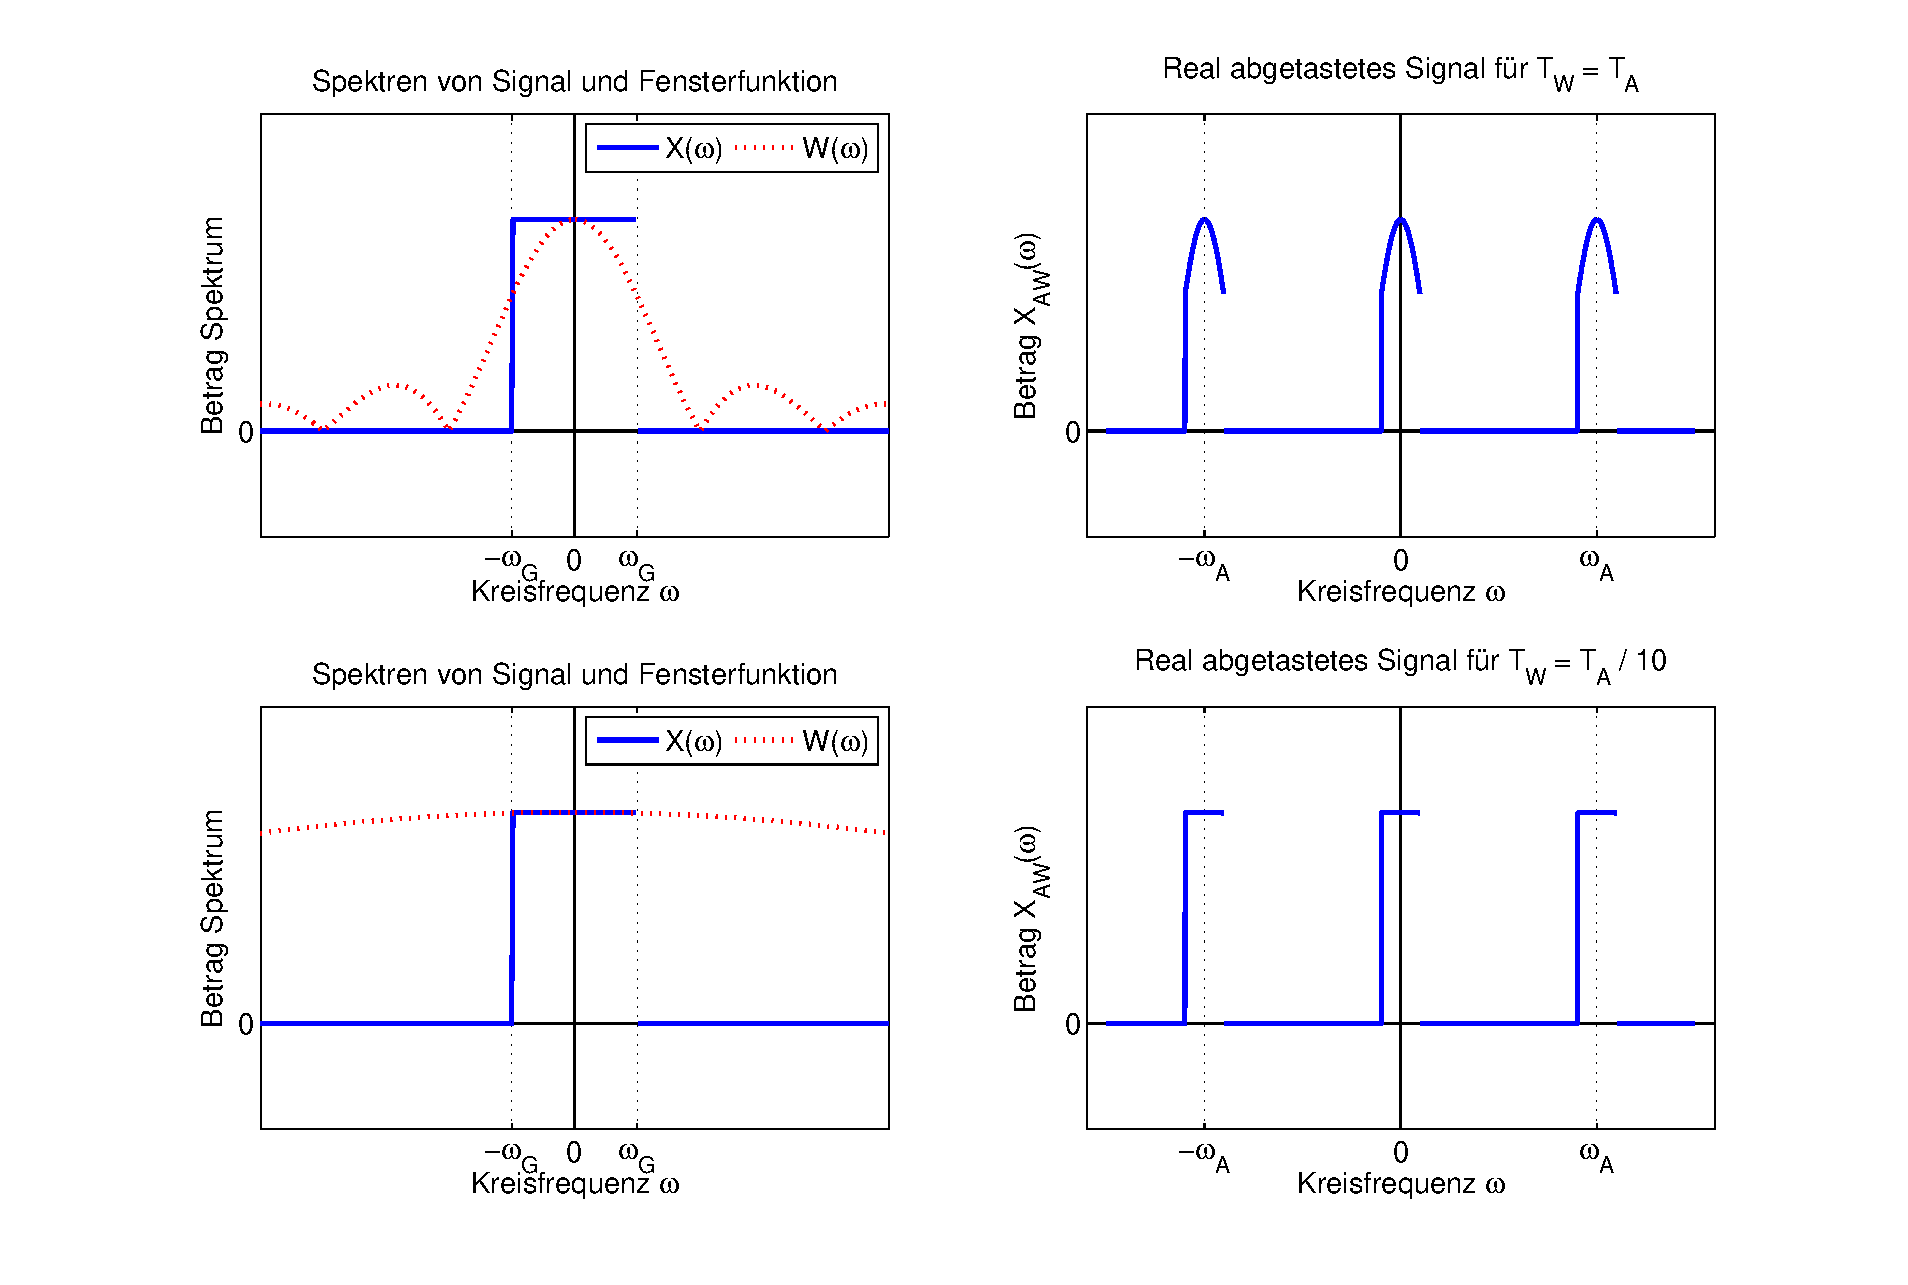
\includegraphics[width=1\textwidth]{Kapitel1/Bilder/image14}}
  \caption{ Darstellung des Spektrums eines realen Abtastprozesses für unterschiedliche Wandlungszeiten T$_{W}$ = T$_{A}$ und T$_{W}$ = 0.1$\cdot$T$_{A}$
}
  \label{fig:AbtastprozessRealSpektrum}
\end{figure}


\subsubsection{Reale Rekonstruktion eines Signals}

\noindent Nach der Abtastung liegen einzelne Abtastwerte vor, die das Signal zu den entsprechenden Abtastzeiten charakterisieren. F\"{u}r einige Anwendungen ist es notwendig, diese zeitdiskreten Signale wieder in zeitkontinuierliche Signale zu wandeln. Die bereits diskutierte ideale Rekonstruktion eines Signals ist wegen des ideal angenommenen Tiefpass-Filters nicht kausal und kann deshalb technisch nicht realisiert werden. Eine technisch realisierbare Rekonstruktion des urspr\"{u}nglichen Signals aus den Abtastwerten wird in zwei Schritten realisiert: 

\begin{itemize}
\item  Erzeugung eines stufenf\"{o}rmigen Ausgangssignals mit einem Halteglied
\item  Tiefpass-Filterung
\end{itemize}

\noindent Die beiden Schritte werden im Zeit- und Frequenzbereich beschrieben. Zur \"{U}bersicht stellt Bild \ref{fig:SignalflussRekonstruktion} den Signalfluss einer realen Signalrekonstruktion bei idealer Signalabtastung dar.

\clearpage
\begin{figure}[H]
  \centerline{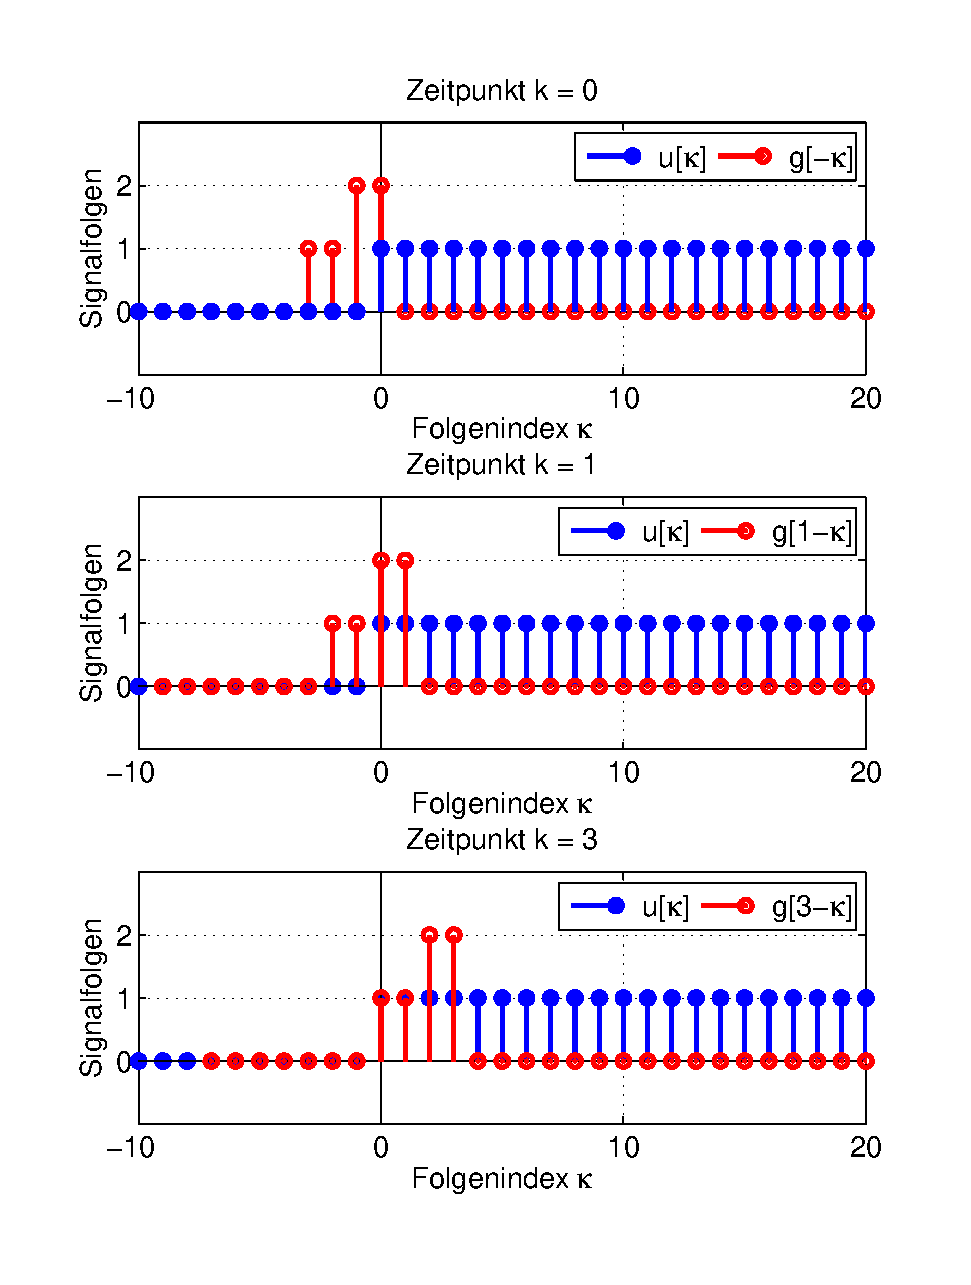
\includegraphics[width=0.4\textwidth]{Kapitel1/Bilder/image15}}
  \caption{Signalfluss zur realen Rekonstruktion}
  \label{fig:SignalflussRekonstruktion}
\end{figure}


{\fontfamily{phv}\selectfont
\noindent\textbf{Erzeugung eines stufenförmigen Ausgangssignals mit einem Halteglied}} \smallskip

\noindent Die einzelnen Abtastwerte stellen das Signal zu den entsprechenden Abtastzeiten dar. Das Halteglied H h\"{a}lt den aktuell g\"{u}ltigen Wert des digitalen Systems am Ausgang fest, bis der n\"{a}chste Abtastwert zur Verf\"{u}gung steht. Dadurch steht zu jedem Zeitpunkt t ein Ausgangssignal zur Verf\"{u}gung und das Signal ist wieder zeitkontinuierlich. Bild \ref{fig:RekonstruktionRealSignal} zeigt an einem Beispiel das abgetastete Signal x${}_{A}$(t) und das Signal x${}_{H}$(t) nach dem Halteglied.

\begin{figure}[H]
  \centerline{\includegraphics[width=1\textwidth]{Kapitel1/Bilder/image16}}
  \caption{Rekonstruktion eines abgetasteten Signals mit Halteglied}
  \label{fig:RekonstruktionRealSignal}
\end{figure}

\noindent Im Zeitbereich kann das kontinuierliche Signal nach dem Halteglied analog zur realen Wandlung mit Rechteckfunktionen beschrieben werden.

\begin{equation}\label{eq:twotwentyseven}
w\left(t\right)=\frac{1}{T_{W} } \cdot \left(\sigma \left(t\right)-\sigma \left(t-T_{W} \right)\right)
\end{equation}

\noindent Das Signal nach dem Halteglied kann wieder als Faltung ausgedr\"{u}ckt werden.

\begin{equation}\label{eq:twotwentyeight}
\begin{split}
x_{H} \left(t\right) & = \sum _{k=-\infty }^{\infty }x_{A} \left(k\cdot T_{A} \right)\cdot  \left(\sigma \left(t-k\cdot T_{A} \right)-\sigma \left(t-\left(k+1\right)\cdot T_{A} \right)\right) \\ 
& = \left(\sum _{k=-\infty }^{\infty }x\left(k\cdot T_{A} \right)\cdot \delta \left(t-k\cdot T_{A} \right) \right)*\left(\sigma \left(t\right)-\sigma \left(t-T_{A} \right)\right)    
\end{split}
\end{equation}

\noindent Der Faltung der Signale im Zeitbereich entspricht die Multiplikation der Spektren im Frequenzbereich. Das Spektrum des Signals nach dem Halteglied ergibt sich damit aus dem Produkt des Spektrums X${}_{A}$($\omega$) und dem Frequenzgang des Halteglieds H($\omega$).

\begin{equation}\label{eq:twotwentynine}
H\left(\omega \right)=\frac{2}{\omega } \cdot \sin \left(\frac{\omega \cdot T_{A} }{2} \right)\cdot e^{-j\cdot \frac{\omega \cdot T_{A} }{2} }
\end{equation}


\noindent Bild \ref{fig:RekonstruktionRealSpektrum} zeigt das Spektrum des abgetasteten Signals x${}_{A}$(t) und dem Signal x${}_{H}$(t) nach dem Halteglied.

\begin{figure}[H]
  \centerline{\includegraphics[width=1\textwidth]{Kapitel1/Bilder/image17}}
  \caption{Betrag des Spektrums vom abgetasteten Signal x${}_{A}$(t) und vom Signal x${}_{H}$(t) nach dem Halteglied}
  \label{fig:RekonstruktionRealSpektrum}
\end{figure}

\noindent Durch das Halteglied wird das Spektrum im Bereich der Grenzfrequenz $\omega_{G}$ ged\"{a}mpft. Diese D\"{a}mpfung wirkt sich aber vor allem auf die periodische Fortsetzung des Spektrums aus. \bigskip

{\fontfamily{phv}\selectfont
\noindent\textbf{Filterung des stufenf\"{o}rmigen Signals}} \smallskip

\noindent Zur Vermeidung von Signalspr\"{u}ngen im rekonstruierten Signal wird das Spektrum nach dem Halteglied mit einem geeigneten Filter gefiltert. Mit der \"{U}bertragungsfunktion dem Frequenzgang des Filters G${}_{R}$($\omega$) ergibt sich der Frequenzgang des rekonstruierten Signals x${}_{R}$(t) zu

\begin{equation}\label{eq:twothirty}
X_{R} \left(\omega \right)=X_{A} \left(\omega \right)\cdot \frac{2}{\omega } \cdot \sin \left(\frac{\omega \cdot T_{A} }{2} \right)\cdot e^{-j\cdot \frac{\omega \cdot T_{A} }{2} } \cdot G_{R} \left(\omega \right)
\end{equation}

\noindent Idealerweise w\"{u}rde das Filter die Abweichungen im Basisband des Nutzsignals - $\omega_{N} \mathrm{<} \omega \mathrm{<} \omega_{N}$ kompensieren und die Frequenzanteile ober- und unterhalb des Basisbandes vollst\"{a}ndig eliminieren. Bild \ref{fig:RekonstruktionTiefpassSpektrum} verdeutlicht diesen Ansatz.

\begin{figure}[H]
  \centerline{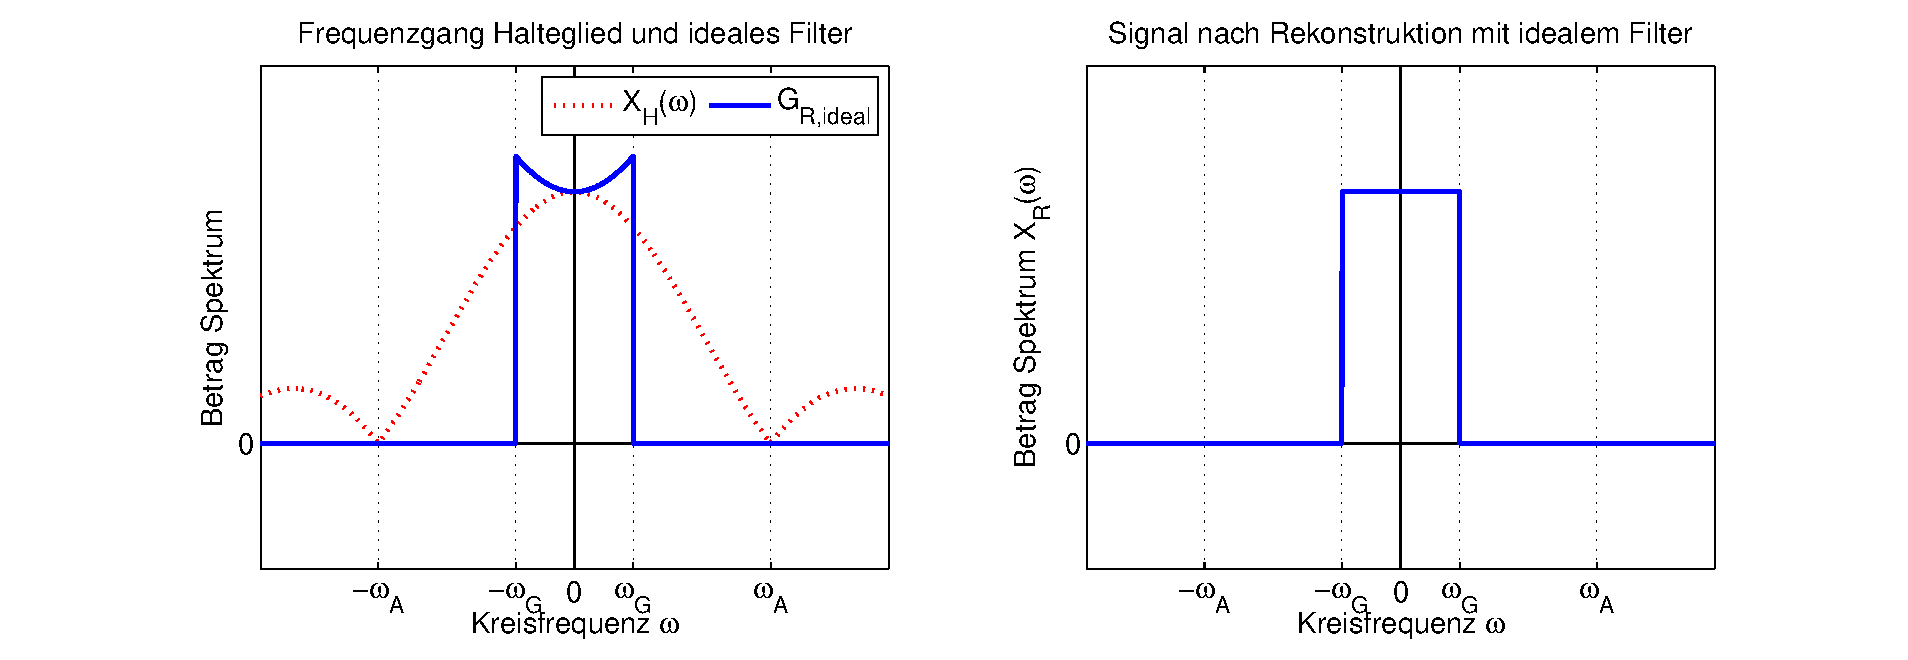
\includegraphics[width=1\textwidth]{Kapitel1/Bilder/image18}}
  \caption{Ideales Filter zur Rekonstruktion eines abgetasteten Signals}
  \label{fig:RekonstruktionTiefpassSpektrum}
\end{figure}

\clearpage

\noindent Dieses ideale Filter ist wegen der idealen Flankensteilheit nicht realisierbar. Reale Filter beschr\"{a}nken sich auf eine endliche Flankensteilheit. Eine M\"{o}glichkeit, die erforderliche Flankensteilheit zu senken, ist eine Steigerung der Abtastrate f${}_{A}$. Dieser Vorgang wird als \"{U}berabtastung oder Oversampling bezeichnet. Durch die h\"{o}here Abtastrate werden zwei Effekte erzielt:

\begin{itemize}
\item  Die Trennung der periodischen Spektren ist gr\"{o}{\ss}er. Dadurch kann die Ordnung des Filters zur Signal-Rekonstruktion reduziert werden.

\item  Mit h\"{o}herer Abtastrate liegt der Nutzbereich des Signals immer mehr im flachen Bereich der \"{U}bertragungsfunktion des Halteglieds, sodass eine Kompensation des Frequenzgangs des Halteglieds nicht weiter notwendig ist.
\end{itemize}

\noindent Die zum Halteglied inverse Charakteristik im Durchlassbereich kann \"{u}ber ein digitales Filter erreicht werden, der als Teil der digitalen Signalverarbeitung realisiert wird. 


\subsubsection{Totzeit bei der realen Signalabtastung}

\noindent In den vorangegangenen Abschnitten wird der Abtastvorgang hinsichtlich der Auswirkung auf den Betrag des Spektrums diskutiert. Die \"{U}bertragungsfunktionen weisen aber immer auch eine Phasenverschiebung auf. Die gesamte Phasenverschiebung ergibt sich bei der realen Abtastung nach den obigen Darstellungen aus den Totzeiten des Wandlers und des Halteglieds.


\begin{equation}\label{eq:twothirtyone}
T_{T} =\frac{T_{W} }{2} +\frac{T_{A} }{2}
\end{equation}

\noindent Dazu kommen die Phase des Anti-Aliasing-Filters und des Tiefpass-Filters zur Signalrekonstruktion, sodass gegen\"{u}ber dem Eingangssignal eine teilweise erhebliche Signalverz\"{o}gerung entsteht. Die Zeitverz\"{o}gerung sowie das Einschwingverhalten des rekonstruierten Signals werden an einem Beispiel verdeutlicht.\bigskip

\noindent
\colorbox{lightgray}{%
\arrayrulecolor{white}%
\renewcommand\arraystretch{0.6}%
\begin{tabular}{ wl{16.5cm} }
{\fontfamily{phv}\selectfont{Beispiel: Signalrekonstruktion} }
\end{tabular}%
}\medskip

\noindent Ein Signal der Form 

\begin{equation}\label{eq:twothirtytwo}
x\left(t\right)=5\cdot e^{-0.1\cdot t^{2} } \cdot \left(1+0.5\cdot \sin \left(t\right)\right)\cdot \left(\sigma \left(t+5\right)-\sigma \left(t-5\right)\right)
\end{equation}

\noindent wird mit einer Abtastzeit von T$_{A}$ = 1 abgetastet, das System besitzt eine Wandlungszeit von T$_{W}$ = 1. Es entstehen die in Tabelle \ref{tab:twoone} dargestellten Abtastwerte.

\clearpage
\begin{table}[H]
\setlength{\arrayrulewidth}{.1em}
\caption{Tabellarische Übersicht über Signaleigenschaften für Signalfolgen}

\setlength{\fboxsep}{0pt}%
\colorbox{lightgray}{%
\arrayrulecolor{white}%
\begin{tabular}{| c | c | c | c | c | c | c | c | c | c | c | c |}
\hline
\parbox[c][0.45in][c]{0.45in}{\smallskip\centering\textbf{\fontfamily{phv}\selectfont{T/T${}_{A}$}}} & 
\parbox[c][0.37in][c]{0.37in}{\centering{-5}} & 
\parbox[c][0.37in][c]{0.37in}{\centering{-4}} & 
\parbox[c][0.37in][c]{0.37in}{\centering{-3}} & 
\parbox[c][0.37in][c]{0.37in}{\centering{-2}} & 
\parbox[c][0.37in][c]{0.37in}{\centering{-1}} & 
\parbox[c][0.37in][c]{0.37in}{\centering{0}} & 
\parbox[c][0.37in][c]{0.37in}{\centering{1}} & 
\parbox[c][0.37in][c]{0.37in}{\centering{2}} & 
\parbox[c][0.37in][c]{0.37in}{\centering{3}} & 
\parbox[c][0.37in][c]{0.37in}{\centering{4}} & 
\parbox[c][0.37in][c]{0.37in}{\centering{5}}\\  \hline
\parbox[c][0.45in][c]{0.45in}{\smallskip\centering\textbf{\fontfamily{phv}\selectfont{x(k$\cdot$T${}_{A}$)}}} & 
\parbox[c][0.37in][c]{0.37in}{\centering{0.607}} & 
\parbox[c][0.37in][c]{0.37in}{\centering{1.392}} & 
\parbox[c][0.37in][c]{0.37in}{\centering{1.889}} & 
\parbox[c][0.37in][c]{0.37in}{\centering{1.828}} & 
\parbox[c][0.37in][c]{0.37in}{\centering{2.621}} & 
\parbox[c][0.37in][c]{0.37in}{\centering{5.000}} & 
\parbox[c][0.37in][c]{0.37in}{\centering{6.428}} & 
\parbox[c][0.37in][c]{0.37in}{\centering{4.875}} & 
\parbox[c][0.37in][c]{0.37in}{\centering{2.176}} & 
\parbox[c][0.37in][c]{0.37in}{\centering{0.628}} & 
\parbox[c][0.37in][c]{0.37in}{\centering{0.214}}\\ \hline

\end{tabular}%
}
\label{tab:twoone}
\end{table}


\noindent Die Abtastwerte werden über ein Halteglied und einen Tiefpass mit einer Zeitkonstante T${}_{TP}$ = 0.5 rekonstruiert. Bild \ref{fig:RekonstruktionRealSignalTiefpass} zeigt das analoge Signal x(t) und das durch Abtastung und Rekonstruktion erzeugte Signal x${}_{TP}$(t) bei Verwendung eines Tiefpass erster Ordnung.

\begin{figure}[H]
  \centerline{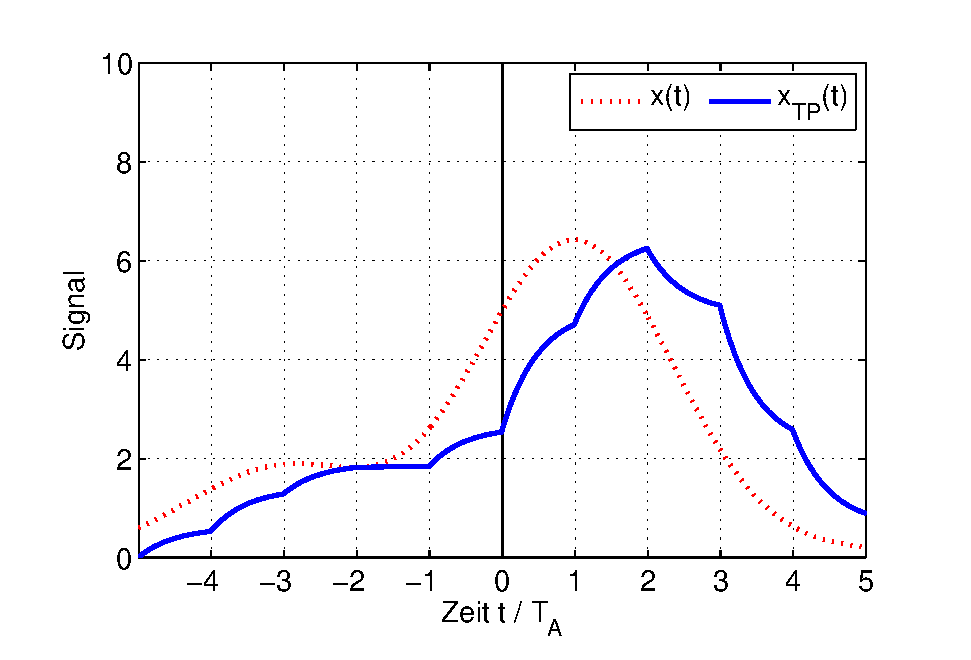
\includegraphics[width=0.5\textwidth]{Kapitel1/Bilder/image19}}
  \caption{Vergleich eines Zeitsignals x(t) und der realen Rekonstruktion des abgetasteten Signals mit einem Tiefpass erster Ordnung}
  \label{fig:RekonstruktionRealSignalTiefpass}
\end{figure}

\noindent Das rekonstruierte Signal weist zum einen eine Verzögerung von

\begin{equation}\label{eq:twothirtythree}
T_{T} =\frac{T_{W} }{2} +\frac{T_{A} }{2} =\frac{T_{A} }{2} +\frac{T_{A} }{2} =T_{A}
\end{equation}

\noindent auf. Au{\ss}erdem ist das Einschwingen des Tiefpasses nach jedem Quantisierungsschritt zu erkennen. 

\noindent Diese Signalverzögerung T${}_{T}$ ist insbesondere bei Regelungssystemen kritisch anzusehen. Auch in dieser Beziehung ist eine hohe Abtastrate, die wegen kleiner Abtastzeit und Wandlungszeit zu einer Verringerung der Totzeit führt, vorteilhaft.

\InsertBoxL{0}{\includegraphics[scale=0.5]{Code.JPG}} 
\textcolor{white}{.}\newline
\noindent Im Online-Portal \textit{Systemtheorie Online} verdeutlicht die \textit{Applikation Signalabtastung und Signal-
rekonstruktion} grafisch, welche Effekte durch Anti-Aliasing-Filter, reale Abtastung und reale Rekon-struktion entstehen.\newline    

\clearpage

\subsection{Literatur}


\subsubsection{Literaturstellen mit besonders anschaulicher Darstellung}

\begin{tabular}{|p{0.8in}|p{5.7in}|} \hline 
[Lyon04] & Lyons, Richard G.: Understanding Digital Signal \newline Processing,Prentice Hall, New Jersey, 2004 \\ \hline 
[Stea99] & Stearns, Samuel: Digitale Verarbeitung analoger Signale,\newline 7. Auflage, Oldenbourg Verlag M\"{u}nchen, 1999 \\ \hline 
\end{tabular}


\subsubsection{Literaturstellen mit praktischen Anwendungen}

\begin{tabular}{|p{0.8in}|p{5.7in}|} \hline 
[Wern08] & Werner, Martin: Signale und Systeme,\newline
Vieweg Studium Technik, Wiesbaden, 2008 \\\hline 
[Meye08] & Meyer, Martin: Signalverarbeitung -- Analoge und digitale Signal, Systeme und Filter,\newline 
Vieweg Studium Technik, Wiesbaden, 2008 \\  \hline 
\end{tabular}


\subsubsection{ Weiterf\"{u}hrende Literatur}

\begin{tabular}{|p{0.8in}|p{3.7in}|} \hline 
[Oppe04] & Oppenheim, Alan: Zeitdiskrete Signalverarbeitung,\newline 2. \"{u}berarbeitete Auflage, Pearson Studium, 2004 \\ \hline 
[Kamm98] & Kammeyer, Karl: Digitale Signalverarbeitung,\newline B.G. Teubner Stuttgart, 1998 \\ \hline 
\end{tabular}


\clearpage

\section{Zeitdiskrete Signale}
\noindent In der Serienfertigung und der automatisierten Messtechnik entsteht eine Vielzahl von Daten. Die Datens\"{a}tze sind oft komplex und un\"{u}bersichtlich, eine Interpretation aller Daten im Detail ist zudem zeitaufw\"{a}ndig. Vor diesem Hintergrund ist es erforderlich, die Daten \"{u}bersichtlich darstellen oder auf Kenngr\"{o}{\ss}en komprimieren zu k\"{o}nnen.\newline

\noindent Als Einstieg in die Statistik besch\"{a}ftigt sich dieses Kapitel deshalb mit der Frage, wie Daten numerisch und grafisch aufbereitet werden k\"{o}nnen. Anschlie{\ss}end wird die zusammenfassende Beschreibung von Datens\"{a}tzen mit Hilfe statistischer Kenngr\"{o}{\ss}en eingef\"{u}hrt. 

\subsection{ Merkmalstypen}

\noindent Der Design For Six Sigma (DFSS) Prozess zeichnet sich dadurch aus, dass \"{u}ber den gesamten Prozess quantitative Methoden eingesetzt werden. Die Ergebnisse sind dabei von definierten Merkmalen abh\"{a}ngig. Die Merkmale k\"{o}nnen unterschiedlicher Natur sein. Vor dem Einsatz statistischer Methoden ist es notwendig, die unterschiedlichen Merkmalstypen zu klassifizieren, da sie einen Einfluss auf die Methodik und die Genauigkeit der Aussage haben. Die f\"{u}r den Design For Six Sigma Prozess relevanten Merkmalstypen lassen sich in stetige und diskrete Gr\"{o}{\ss}en, sowie ordinale und gruppierende Gr\"{o}{\ss}en aufteilen. 

\subsubsection{Stetige Merkmale}

\noindent Stetige Merkmale k\"{o}nnen eine Eigenschaft beliebig fein wiedergeben. Es entsteht kein Fehler durch die Darstellung des Ergebnisses, allenfalls durch die Aufzeichnung des Messergebnisses. Beispiele f\"{u}r stetige Merkmale sind Temperaturen, elektrische Spannungen und Str\"{o}me, geometrische Ma{\ss}e wie Strecken oder Fl\"{a}cheninhalte sowie die Zeit. Stetige Merkmale werden bei einer Verarbeitung der Werte im Rechner diskretisiert. Sind die Stufen der Diskretisierung eine Gr\"{o}{\ss}enordnung kleiner als die kleinste darzustellende Gr\"{o}{\ss}e, kann die Quantisierung vernachl\"{a}ssigt werden. Die Merkmale werden als quasi-stetig bezeichnet.


\subsubsection{Diskrete Merkmale}

\noindent Diskrete Merkmale haben nur endlich viele Auspr\"{a}gungen. Zum Beispiel kann ein Wurf mit einem W\"{u}rfel nur die Zahlen eins bis sechs annehmen, und er weist nur endlich viele unterschiedliche Ereignisse auf. Eine Erfassung von stetigen Gr\"{o}{\ss}en mit diskreten Messmitteln f\"{u}hrt zu einer diskreten Messgr\"{o}{\ss}e. Beispielsweise f\"{u}hrt die Messung einer Spannung mit einem 6 Bit Analog-Digital-Wandler und einem Messbereich von 5 V zu einem Quantisierungsintervall von 

\begin{equation}\label{eq:threeone}
\Delta U=\dfrac{5 V}{2^{6} } =78 mV
\end{equation}

\noindent Ist diese Diskretisierung gr\"{o}{\ss}er als ein Zehntel der interessierenden kleinsten Spannung, wird das urspr\"{u}nglich stetige Merkmal als diskretes Merkmal bezeichnet. \newline

\noindent Ein diskretes Merkmal entsteht auch bei der Klassenbildung von stetigen Merkmalen. Zum Beispiel ist es denkbar, die Rohwerte einer Widerstandsmessung in Klassen zusammenzufassen, die einem Widerstandsbereich entsprechen. Nach der Klassenbildung kann nicht mehr entschieden werden, ob der Widerstand am unteren oder oberen Ende des Intervalls lag. Aus dem stetigen Merkmal ist durch die Klassenbildung ein diskretes Merkmal entstanden.

\subsubsection{Ordinale Merkmale}

\noindent Ordinale Datentypen werden f\"{u}r Daten verwendet, die nach ihrer Auspr\"{a}gung geordnet werden k\"{o}nnen, deren Abst\"{a}nde aber nicht interpretiert werden k\"{o}nnen. Ein typisches Beispiel daf\"{u}r sind Kontrollergebnisse, die zu einer Aussage ,,gut``, ,,m\"{a}{\ss}ig`` oder ,,schlecht`` f\"{u}hren. Diese Aussage kann in Zahlen wiedergegeben werden, zum Beispiel kann der Eigenschaft ,,gut`` die Zahl 1, ,,m\"{a}{\ss}ig`` die Zahl 2 und ,,schlecht`` die Zahl 3 zugeordnet werden. Diese Zuordnung gibt jedoch nur ein Ordnungsschema an. Im Gegensatz zu den stetigen und diskreten Datentypen kann mit ordinalen Datentypen nicht sinnvoll gerechnet werden, vielleicht mit Ausnahme der Fuzzy Logik. Au{\ss}erdem sind die Aussagen ,,gut``, ,,m\"{a}{\ss}ig`` oder ,,schlecht`` deutlich gr\"{o}ber und schlechter zu interpretieren als numerische Angaben mit stetigen oder diskreten Daten.


\subsubsection{Gruppierende Merkmale}

\noindent Gruppierende Merkmale sind zum Beispiel bei der Charakterisierung von Verfahren zu finden. Wird ein Verfahren ge\"{a}ndert, erfolgt ein Vergleich des alten Verfahrens mit dem neuen. Auch Zulieferer lassen sich nicht ordnen, sie existieren parallel und k\"{o}nnen nicht nach einer Auspr\"{a}gung geordnet werden. Gruppierende Merkmale werden deshalb im Allgemeinen auch nicht mit Zahlen bezeichnet. 


\subsubsection{Merkmalstypen und Aussagesicherheit}

\noindent Aus der Beschreibung der unterschiedlichen Merkmalstypen ergibt sich, dass die Genauigkeit bei Messungen von stetigen Merkmalen zu gruppierenden Merkmalen kontinuierlich abnimmt. Ordinalen und gruppierenden Datentypen kann eine mathematisch berechnete Kenngr\"{o}{\ss}e nicht mehr sinnvoll zugeordnet werden. Aus diesem Grund unterscheiden sich auch die statistischen Methoden, die f\"{u}r die stetigen und diskreten Datentypen eingesetzt werden, von denen, die f\"{u}r die ordinalen und gruppierten Datentypen verwendet werden. 

\noindent Der Schwerpunkt liegt in den folgenden Kapiteln auf stetigen und diskreten Datentypen, die nur von einer Einflussgr\"{o}{\ss}e abh\"{a}ngen. 

\clearpage

\subsection{H\"{a}ufigkeitsverteilungen}

\noindent Statistische Daten werden durch Aufzeichnen von Beobachtungsergebnissen gewonnen. Die dabei entstehende Liste wird als Urliste bezeichnet. Tabelle \ref{tab:threeone} stellt die Messwerte von N = 100 Widerst\"{a}nden mit einem Sollwert von $R = 1 k\Omega$ dar. Die Daten weisen eine Aufl\"{o}sung von $\Delta R = 1 \Omega$ auf. Es handelt sich deshalb um einen diskreten Merkmalstyp.

\begin{table}[H]
\setlength{\arrayrulewidth}{.1em}
\caption{Beispiel f\"{u}r eine Urliste: Messwerte von 100 Widerst\"{a}nden mit einem Sollwert von $R = 1 k \Omega $}
\setlength{\fboxsep}{0pt}%
\colorbox{lightgray}{%
\arrayrulecolor{white}%
\begin{tabular}{| wc{2cm} | wc{1cm} | wc{1cm} | wc{1cm} | wc{1cm} | wc{1cm} | wc{1cm} | wc{1cm} | wc{1cm} | wc{1cm} | wc{1cm} }
\hline\xrowht{15pt}

\fontfamily{phv}\selectfont\textbf{Index} & \multicolumn{10}{c}{\fontfamily{phv}\selectfont\textbf{Messwert R / $\Omega$}} \\ \hline \xrowht{15pt}

\fontfamily{phv}\selectfont\textbf{1 - 10} &
983 & 988 & 985 & 987 & 988 & 987 & 986 & 985 & 986 & 991\\ \hline\xrowht{15pt}

\fontfamily{phv}\selectfont\textbf{11 - 20} & 
987 & 986 & 987 & 986 & 985 & 988 & 986 & 986 & 988 & 985\\ \hline\xrowht{15pt}

\fontfamily{phv}\selectfont\textbf{21 - 30} &
985 & 989 & 986 & 986 & 985 & 992 & 988 & 989 & 986 & 986\\ \hline\xrowht{15pt}

\fontfamily{phv}\selectfont\textbf{31 - 40} &
985 & 986 & 986 & 986 & 989 & 988 & 986 & 986 & 986 & 987\\ \hline\xrowht{15pt}

\fontfamily{phv}\selectfont\textbf{41 - 50} &
989 & 986 & 986 & 985 & 988 & 990 & 986 & 986 & 988 & 987\\ \hline\xrowht{15pt}

\fontfamily{phv}\selectfont\textbf{51 - 60} &
985 & 989 & 987 & 985 & 986 & 990 & 986 & 985 & 986 & 988\\ \hline\xrowht{15pt}

\fontfamily{phv}\selectfont\textbf{61 - 70} &
985 & 988 & 984 & 988 & 986 & 985 & 987 & 989 & 986 & 987\\ \hline\xrowht{15pt}

\fontfamily{phv}\selectfont\textbf{71 - 80} &
987 & 987 & 985 & 987 & 986 & 986 & 986 & 987 & 985 & 989\\ \hline\xrowht{15pt}

\fontfamily{phv}\selectfont\textbf{81 - 90} &
988 & 992 & 985 & 986 & 987 & 987 & 985 & 988 & 984 & 988\\ \hline\xrowht{15pt}

\fontfamily{phv}\selectfont\textbf{91 - 100} &
987 & 988 & 985 & 986 & 986 & 985 & 987 & 989 & 986 & 985\\ \hline
\end{tabular}%
}
\label{tab:threeone}
\end{table}

\noindent Die in Tabelle \ref{tab:threeone} dargestellten Gr\"{o}{\ss}en bilden eine Stichprobe mit dem Umfang N = 100, die einzelnen Messwerte werden allgemein als Stichprobenwerte bezeichnet. Mithilfe der Wahrscheinlichkeitsrechnung wird sp\"{a}ter versucht, von der Stichprobe auf die Grundgesamtheit, zum Beispiel aller Widerst\"{a}nde in einem definierten Fertigungszeitraum, zu schlie{\ss}en. \newline

\noindent Zur \"{U}bersicht k\"{o}nnen die Daten in einem sogenannten Streudiagramm dargestellt werden. Dabei wird der Stichprobenindex als Abszisse und der Stichprobenwert als Ordinate dargestellt. 

\noindent 
\begin{figure}[H]
  \centerline{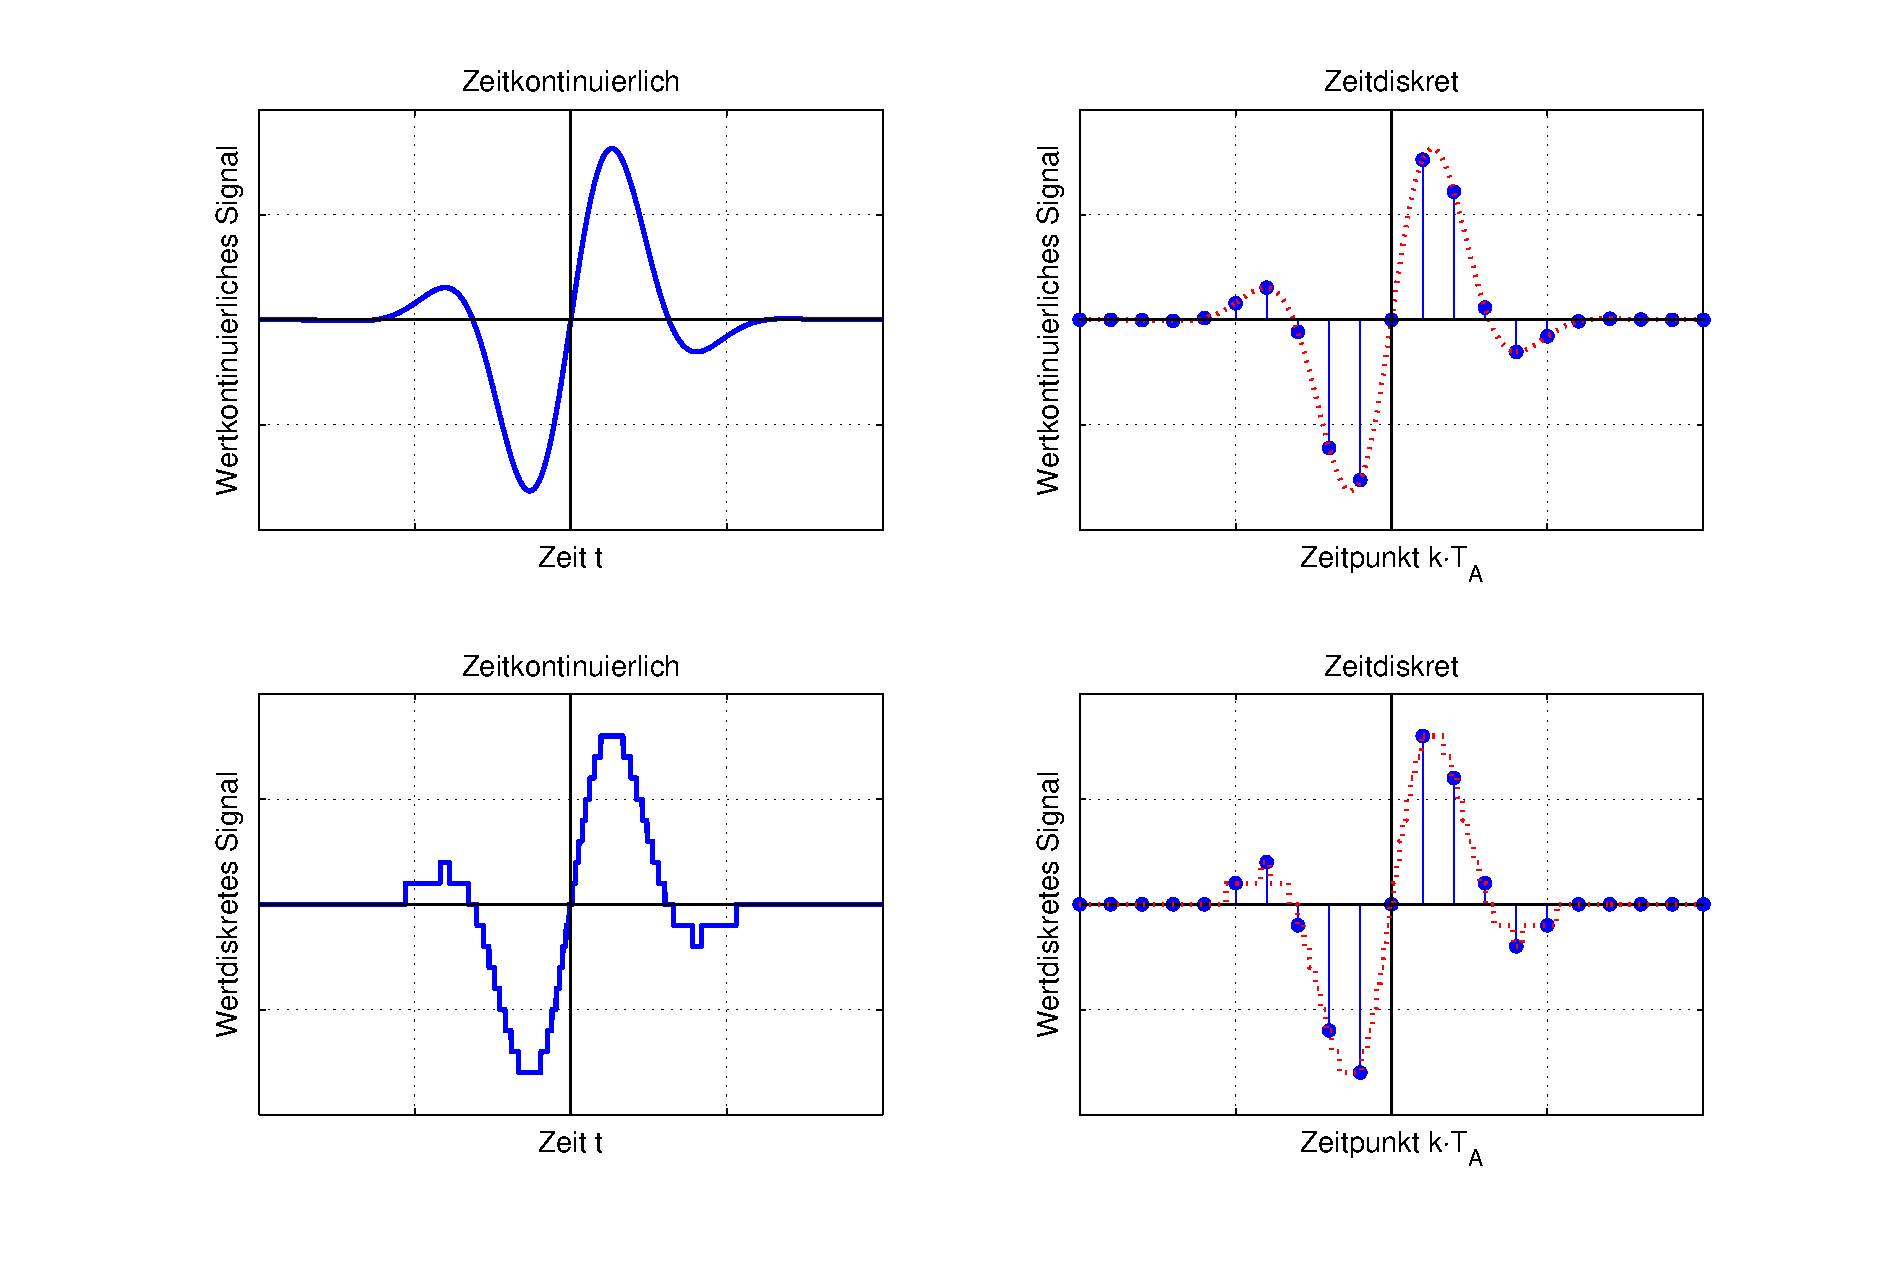
\includegraphics[width=0.5\textwidth]{Kapitel3/Bilder/image1}}
  \caption{Darstellung der Stichprobe in Tabelle \ref{tab:threeone} als Streudiagramm}
  \label{fig:RelHaeufigkeitUndSummenhStichprobeWiderstand1}
\end{figure}

\subsubsection{Absolute und relative H\"{a}ufigkeit diskreter Merkmalstypen}\label{threetwoone}

\noindent Zur \"{u}bersichtlichen Darstellung der Stichprobenwerte diskreter Merkmalstypen werden die Stichproben der Gr\"{o}{\ss}e nach geordnet, und die H\"{a}ufigkeit der einzelnen Werte wird ausgewertet. Bei manueller Ausf\"{u}hrung ergibt sich zun\"{a}chst eine Strichliste wie in Tabelle \ref{tab:threetwo}, aus der anschlie{\ss}end eine H\"{a}ufigkeitsverteilung wie in Tabelle 3.3 abgeleitet werden kann.


\begin{table}[H]
\caption{H\"{a}ufigkeitsbewertung \"{u}ber eine Strichliste }
\setlength{\fboxsep}{0pt}%
\colorbox{lightgray}{%
\arrayrulecolor{white}%
\begin{tabular}{| c | c | c | c |}
\hline
\parbox[c][0.28in][c]{1in}{\smallskip\centering\textbf{\fontfamily{phv}\selectfont{R / $\mathbf{\Omega}$}}} & 
\parbox[c][0.28in][c]{2.1in}{\smallskip\centering\textbf{\fontfamily{phv}\selectfont{Absolute H\"{a}ufigkeit h$_{\mathbf{A}}$(R)}}} &
\parbox[c][0.28in][c]{1in}{\smallskip\centering\textbf{\fontfamily{phv}\selectfont{R / $\mathbf{\Omega}$}}} &
\parbox[c][0.28in][c]{2.1in}{\smallskip\centering\textbf{\fontfamily{phv}\selectfont{Absolute H\"{a}ufigkeit h$_{\mathbf{A}}$(R)}}}\\ \hline

\parbox[c][0.28in][c]{1in}{\centering\fontfamily{phv}\selectfont{983}} &
\parbox[c][0.28in][c]{2.1in}{\centering{I}} &
\parbox[c][0.28in][c]{1in}{\centering\fontfamily{phv}\selectfont{988}} &
\parbox[c][0.28in][c]{2.1in}{\centering{IIII IIII IIII}} \\ \hline

\parbox[c][0.28in][c]{1in}{\centering\fontfamily{phv}\selectfont{984}} &
\parbox[c][0.28in][c]{2.1in}{\centering{II}} &
\parbox[c][0.28in][c]{1in}{\centering\fontfamily{phv}\selectfont{989}} &
\parbox[c][0.28in][c]{2.1in}{\centering{IIII III}} \\ \hline

\parbox[c][0.28in][c]{1in}{\centering\fontfamily{phv}\selectfont{985}} &
\parbox[c][0.28in][c]{2.1in}{\centering{IIII IIII IIII IIII}} &
\parbox[c][0.28in][c]{1in}{\centering\fontfamily{phv}\selectfont{990}} &
\parbox[c][0.28in][c]{2.1in}{\centering{II}} \\ \hline

\parbox[c][0.28in][c]{1in}{\centering\fontfamily{phv}\selectfont{986}} &
\parbox[c][0.28in][c]{2.1in}{\centering{IIII IIII IIII IIII IIII IIII II}} &
\parbox[c][0.28in][c]{1in}{\centering\fontfamily{phv}\selectfont{991}} &
\parbox[c][0.28in][c]{2.1in}{\centering{I}} \\ \hline

\parbox[c][0.28in][c]{1in}{\centering\fontfamily{phv}\selectfont{987}} &
\parbox[c][0.28in][c]{2.1in}{\centering{IIII IIII IIII II}} &
\parbox[c][0.28in][c]{1in}{\centering\fontfamily{phv}\selectfont{992}} &
\parbox[c][0.28in][c]{2.1in}{\centering{II}} \\ \hline

\end{tabular}%
}\bigskip
\label{tab:threetwo}
\end{table}

\begin{table}[H]
\caption{Häufigkeitsverteilung der Stichprobe}
\setlength{\fboxsep}{0pt}%
\colorbox{lightgray}{%
\arrayrulecolor{white}%
\begin{tabular}{| c | c | c | c | c | c |}
\hline
\parbox[c][0.7in][c]{0.97in}{\smallskip\centering\textbf{\fontfamily{phv}\selectfont{R / $\mathbf{\Omega}$}}} & 
\parbox[c][0.7in][c]{0.97in}{\smallskip\centering\textbf{\fontfamily{phv}\selectfont{Absolute\\ H\"{a}ufigkeit\\ h$_{\mathbf{A}}$(R)}}} &
\parbox[c][0.7in][c]{0.97in}{\smallskip\centering\textbf{\fontfamily{phv}\selectfont{Relative\\ H\"{a}ufigkeit\\ h$_{\mathbf{A}}$(R)}}} &
\parbox[c][0.7in][c]{0.97in}{\smallskip\centering\textbf{\fontfamily{phv}\selectfont{R / $\mathbf{\Omega}$}}} &
\parbox[c][0.7in][c]{0.97in}{\smallskip\centering\textbf{\fontfamily{phv}\selectfont{Absolute\\ H\"{a}ufigkeit\\ h$_{\mathbf{A}}$(R)}}} &
\parbox[c][0.7in][c]{0.97in}{\smallskip\centering\textbf{\fontfamily{phv}\selectfont{Relative\\ H\"{a}ufigkeit\\ h$_{\mathbf{A}}$(R)}}}\\ \hline

\parbox[c][0.28in][c]{0.97in}{\centering{983}} &
\parbox[c][0.28in][c]{0.97in}{\centering{1}} &
\parbox[c][0.28in][c]{0.97in}{\centering{0.01}} &
\parbox[c][0.28in][c]{0.97in}{\centering{988}} &
\parbox[c][0.28in][c]{0.97in}{\centering{15}} &
\parbox[c][0.28in][c]{0.97in}{\centering{0.15}} \\ \hline

\parbox[c][0.28in][c]{0.97in}{\centering{984}} &
\parbox[c][0.28in][c]{0.97in}{\centering{2}} &
\parbox[c][0.28in][c]{0.97in}{\centering{0.02}} &
\parbox[c][0.28in][c]{0.97in}{\centering{989}} &
\parbox[c][0.28in][c]{0.97in}{\centering{8}} &
\parbox[c][0.28in][c]{0.97in}{\centering{0.08}} \\ \hline

\parbox[c][0.28in][c]{0.97in}{\centering{985}} &
\parbox[c][0.28in][c]{0.97in}{\centering{20}} &
\parbox[c][0.28in][c]{0.97in}{\centering{0.20}} &
\parbox[c][0.28in][c]{0.97in}{\centering{990}} &
\parbox[c][0.28in][c]{0.97in}{\centering{2}} &
\parbox[c][0.28in][c]{0.97in}{\centering{0.02}} \\ \hline

\parbox[c][0.28in][c]{0.97in}{\centering{986}} &
\parbox[c][0.28in][c]{0.97in}{\centering{32}} &
\parbox[c][0.28in][c]{0.97in}{\centering{0.32}} &
\parbox[c][0.28in][c]{0.97in}{\centering{991}} &
\parbox[c][0.28in][c]{0.97in}{\centering{1}} &
\parbox[c][0.28in][c]{0.97in}{\centering{0.01}} \\ \hline

\parbox[c][0.28in][c]{0.97in}{\centering{987}} &
\parbox[c][0.28in][c]{0.97in}{\centering{17}} &
\parbox[c][0.28in][c]{0.97in}{\centering{0.17}} &
\parbox[c][0.28in][c]{0.97in}{\centering{992}} &
\parbox[c][0.28in][c]{0.97in}{\centering{2}} &
\parbox[c][0.28in][c]{0.97in}{\centering{0.02}} \\ \hline

\end{tabular}%
}\bigskip
\label{tab:threethree}
\end{table}

\noindent Die absolute H\"{a}ufigkeit gibt an, wie oft der entsprechende Messwert x in der Stichprobe die Auspr\"{a}gung $x{}_{n}$ annimmt. Diese Anzahl wird als absolute H\"{a}ufigkeit $h{}_{A}(x)$ bezeichnet. Die relative H\"{a}ufigkeit $h(x)$ ergibt sich aus dem Quotient aus absoluter H\"{a}ufigkeit $h{}_{A}$(x) und dem Stichprobenumfang~N.

\begin{equation}\label{eq:threetwo}
h(x)=\dfrac{h_{A} (x)}{N} 
\end{equation}

\noindent Zum Beispiel kommt die Auspr\"{a}gung mit einem Widerstandswert von $R = 988 \Omega$ in der Stichprobe 15-mal vor. Da die Stichprobe insgesamt $N = 100$ Werte aufweist, ergibt sich eine relative H\"{a}ufigkeit von $15 \%$.

\noindent Kommt der Wert $x_{0}$ in der Stichprobe nicht vor, hat er die absolute H\"{a}ufigkeit $h_{A}(x_{0})$ = 0 und nach Gleichung \eqref{eq:twothirtyseven} auch die relative H\"{a}ufigkeit $h(x_{0}) = 0$. Im anderen Extremfall k\"{o}nnten alle Stichprobenwerte die Auspr\"{a}gung $x_{1}$ haben. In diesem Fall w\"{a}re die absolute H\"{a}ufigkeit $h_{A}(x_{1}) = N$ und damit die relative H\"{a}ufigkeit $h(x_{1}) = 1$. Die relative H\"{a}ufigkeit $h(x)$ ist somit eine nicht negative Zahl, die h\"{o}chstens den Wert 1 annehmen kann.

\begin{equation}\label{eq:threethree}
0\le h(x)\le 1
\end{equation}

\noindent Die Zahlenwerte in Tabelle \ref{tab:threethree} stellen die H\"{a}ufigkeitsverteilung h(x) der Stichprobe dar. Sie ordnet jedem Wert x eine relative H\"{a}ufigkeit h(x) zu. Die Summe aller absoluten H\"{a}ufigkeiten muss die Anzahl von Stichprobenwerten N ergeben. Die Summe aller relativen H\"{a}ufigkeiten ist damit 1. Es gilt: 

\begin{equation}\label{eq:threefour}
h(x_{1})+h(x_{2} )+h)+{\rm \; ...\; }+h(x_{N})=\sum _{n=1}^{N}h(x_{n} )=1
\end{equation}

\noindent Zur besseren \"{U}bersicht k\"{o}nnen die absolute oder die relative H\"{a}ufigkeit in Form von Stab- oder Liniendiagrammen dargestellt werden. Bild \ref{fig:HaeufigkeitStichprobeWiderstand} stellt die relative H\"{a}ufigkeit f\"{u}r die Stichprobe in Tabelle \ref{tab:threeone} als Histogramm dar.

\noindent 
\begin{figure}[H]
  \centerline{\includegraphics[width=0.5\textwidth]{Kapitel3/Bilder/image2}}
  \caption{Darstellung der relativen H\"{a}ufigkeiten als Stabdiagramm f\"{u}r die Stichprobe in Tabelle \ref{tab:threeone}}
  \label{fig:HaeufigkeitStichprobeWiderstand}
\end{figure}

\noindent Bei sehr vielen unterschiedlichen Zahlenwerten der Stichprobe wird die H\"{a}ufigkeitsverteilung un\"{u}bersichtlich. Aus diesem Grund k\"{o}nnen die Stichprobenwerte in Klassen eingeteilt werden. Ausgehend von dem Gesamtintervall, in dem die Stichprobenwerte liegen, werden Teilintervalle oder Klassenintervalle gebildet. Die Mittenwerte $c_{n}$ der Intervalle hei{\ss}en Klassenmitten. Die einzelnen Stichprobenwerte werden den entsprechenden Teilintervallen oder Klassen zugeordnet. Es ergibt sich die absolute und analog zu Gleichung \eqref{eq:threetwo} die relative Klassenh\"{a}ufigkeit. Die H\"{a}ufigkeit in Abh\"{a}ngigkeit der Klassenmitten hei{\ss}t H\"{a}ufigkeitsverteilung der in Klassen eingeteilten Stichprobe.\newline

\noindent Nach der Aufteilung in Klassen treten die urspr\"{u}nglichen Stichprobenwerte nicht mehr einzeln in Erscheinung, sie gehen nur als Summe in die H\"{a}ufigkeitsverteilung der in Klassen eingeteilten Stichprobe ein. Je weniger Klassen gebildet werden, desto mehr Information geht verloren. Eine ungeeignete Anzahl oder Einteilung von Klassen f\"{u}hrt zu un\"{u}bersichtlichen oder falschen Interpretationsergebnissen. Bei der Definition von Stichprobenklassen haben sich folgende Regeln als sinnvoll erwiesen:

\begin{itemize}
    \item  Die Klassenintervalle sind gleich gro{\ss} zu w\"{a}hlen.
    \item  Die Klassenmitten sollen m\"{o}glichst einfache Zahlen mit m\"{o}glichst wenigen Ziffern sein.
    \item  Die Anzahl von Klassen sollte zwischen 10 und 20 liegen, sinnvoll ist eine Anzahl von Klassen mit 
\end{itemize}

\begin{equation}\label{eq:threefive}
Anzahl\approx \sqrt{N}
\end{equation}

\noindent Werden die Widerstandswerte aus Tabelle \ref{tab:threeone} in drei oder sechs Klassen eingeteilt, ergibt sich die in Bild \ref{fig:HaeufigkeitStichprobeWiderstandKlassen} dargestellte relative H\"{a}ufigkeit.

\noindent 
\begin{figure}[H]
  \centerline{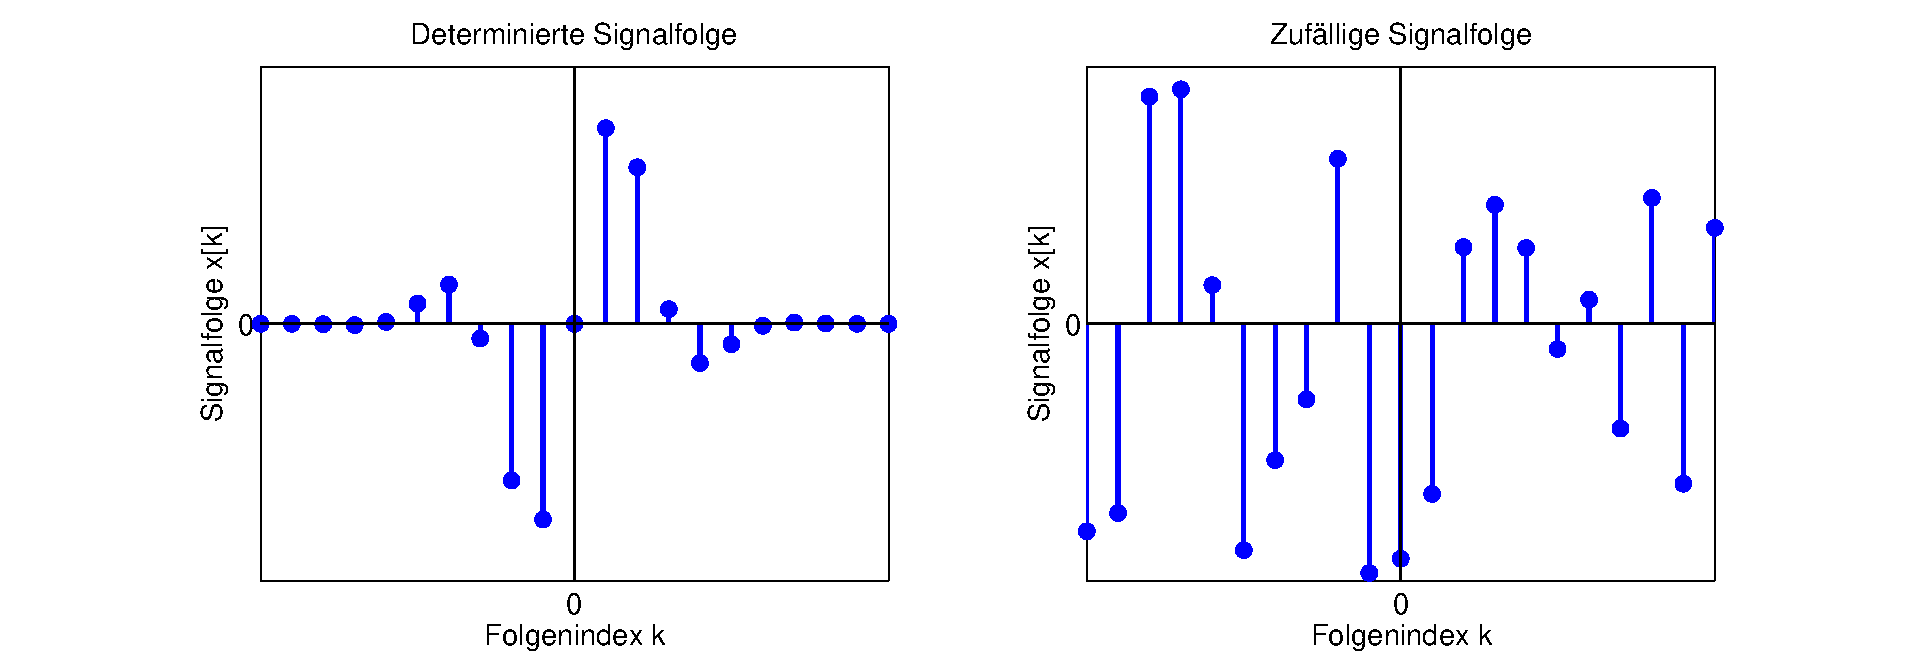
\includegraphics[width=1\textwidth]{Kapitel3/Bilder/image3}}
  \caption{Darstellung der relativen H\"{a}ufigkeiten f\"{u}r die Stichprobe in Tabelle \ref{tab:threeone}}
  \label{fig:HaeufigkeitStichprobeWiderstandKlassen}
\end{figure}

\noindent Dabei wird bei der Darstellung im Stabdiagramm das Prinzip der Fl\"{a}chentreue eingehalten. Es besagt, dass die Fl\"{a}chen direkt proportional zu den absoluten beziehungsweise relativen H\"{a}ufigkeiten sein m\"{u}ssen. Wird der Abstand zwischen zwei benachbarten Klassenmitten $c_{n}$ und $c_{n-1}$ als Breite d mit 

\begin{equation}\label{eq:threesix}
d=c_{n} -c_{n-1}
\end{equation}

\noindent bezeichnet, so muss die H\"{o}he $h_{n}$ im Stabdiagramm den Wert 

\begin{equation}\label{eq:threeseven}
h_{n} =\dfrac{h\left(x_{n} \right)}{d}
\end{equation}

\noindent aufweisen, damit die Fl\"{a}che proportional zur relativen H\"{a}ufigkeit wird

\begin{equation}\label{eq:threeeight}
A_{n} =h_{n} \cdot d=\dfrac{h(x_{n})}{d} \cdot d=h(x_{n})
\end{equation}

\subsubsection{Absolute und relative Summenh\"{a}ufigkeit diskreter Merkmalstypen}\label{threetwotwo}

\noindent Die H\"{a}ufigkeitsverteilung h(x) der Stichprobe gibt die relativen H\"{a}ufigkeiten an, mit der die einzelnen Zahlenwerte in der Stichprobe vorkommen. Oft stellt sich aber die Frage, wie viele Stichprobenwerte unter oder auf einem Grenzwert liegen. Soll zum Beispiel f\"{u}r das Beispiel aus Tabelle \ref{tab:threeone} die Frage beantwortet werden, wie viele Widerst\"{a}nde kleiner oder gleich 985 $\Omega$ sind, muss die Summe

\begin{equation}\label{eq:threenine}
h(R\le 985 \Omega) = h(R=983 \Omega )+h(R=984 \Omega)+h(R=985\Omega )=0.23
\end{equation}

\noindent ausgewertet werden. Wird diese Summe f\"{u}r beliebige Werte x durchgef\"{u}hrt, ergibt sich die relative Summenh\"{a}ufigkeit H(x) der Stichprobe. H(x) ist die Summe der relativen H\"{a}ufigkeiten aller Stichprobenwerte, die kleiner oder gleich dem Wert x sind.

\begin{equation}\label{eq:threeten}
H(x)=\sum _{x_{n} =-\infty }^{x}h(x_{n})
\end{equation}

\noindent Bild \ref{fig:RelHaeufigkeitUndSummenhStichprobeWiderstand2} stellt die relative H\"{a}ufigkeit h(R) und die relative Summenh\"{a}ufigkeit H(R) f\"{u}r das Beispiel aus Tabelle \ref{tab:threeone} als Stabdiagramm dar.

\noindent 
\begin{figure}[H]
  \centerline{\includegraphics[width=1\textwidth]{Kapitel3/Bilder/image4}}
  \caption{Darstellung der relativen H\"{a}ufigkeit und Summenh\"{a}ufigkeit f\"{u}r die Stichprobe in Tabelle \ref{tab:threeone}}
  \label{fig:RelHaeufigkeitUndSummenhStichprobeWiderstand2}
\end{figure}

\noindent Die relative Summenh\"{a}ufigkeit erscheint zun\"{a}chst weniger anschaulich. In Abschnitt 3.2.3 wird sich aber zeigen, dass sie bei dem \"{U}bergang zu kontinuierlichen Stichprobenwerten einige Vorteile hat. Der Informationsgehalt ist bei der relativen H\"{a}ufigkeit und der relativen Summenh\"{a}ufigkeit identisch. Nach Gleichung \eqref{eq:threeten} kann die Summenh\"{a}ufigkeit aus der relativen H\"{a}ufigkeit berechnet werden.

\begin{equation}\label{eq:threeeleven}
H(x)=\sum _{x_{n} =-\infty }^{x}h(x_{n})
\end{equation}

\noindent Die Summenh\"{a}ufigkeit f\"{u}r den Wert (x -- d) ergibt sich entsprechend aus

\begin{equation}\label{eq:threetwelve}
H(x-d)=\sum _{x_{n} =-\infty }^{x-d}h(x_{n})
\end{equation}

\noindent Damit kann h(x) bestimmt werden aus der Differenz

\begin{equation}\label{eq:threethirteen}
h(x)=H(x)-H(x-d)
\end{equation}

\noindent Die Darstellungen k\"{o}nnen also mithilfe dieser Gleichungen ineinander \"{u}berf\"{u}hrt werden.

\subsubsection{Beschreibung stetiger Merkmalstypen}

\noindent Die anschauliche Beschreibung von Merkmalen mit einer relativen H\"{a}ufigkeit versagt bei stetigen Merkmalstypen, weil die Messwerte beliebig fein aufgel\"{o}st sind und jeder Messwert typischerweise nur einmal vorkommt. Liegen Stichproben mit stetigen Merkmalen vor, k\"{o}nnen die Werte gruppiert werden. Damit ergibt sich eine Auswertung, wie sie in den Abschnitten \ref{threetwoone} und \ref{threetwotwo} beschrieben ist. Allerdings gehen mit der Gruppierung der Merkmale Informationen verloren.\newline

\noindent Alternativ k\"{o}nnen stetige Merkmale mit einer relativen Summenh\"{a}ufigkeit beschrieben werden. Jeder Stichprobenwert einer Stichprobe mit stetigen Merkmalen kommt wegen der beliebig hohen Aufl\"{o}sung nur einmal vor. Bei einem Stichprobenumfang von N Werten weist jeder dieser Werte eine relative H\"{a}ufigkeit von 1/N auf. Alle anderen Werte weisen die relative H\"{a}ufigkeit von 0 auf. Durch Sortieren der Werte x nach der Gr\"{o}{\ss}e ergibt sich eine geordnete Stichprobe. Die relative Summenh\"{a}ufigkeit der Stichprobe ergibt sich aus 

\begin{equation}\label{eq:threefourteen}
H(x)=\sum _{x_{n} =-\infty }^{x}h(x_{n}) =\sum _{x_{n} =-\infty }^{x}\dfrac{1}{N}
\end{equation}

\noindent Je nach Werteverlauf der Stichprobe ergibt sich eine relative Summenh\"{a}ufigkeit, die grafisch als Liniendiagramm dargestellt werden kann. 

\noindent Bild \ref{fig:AuswertungDrucksensor} vergleicht die beiden Vorgehensweisen. Im linken Bildteil werden die Toleranzwerte einer Stichprobe mit N = 1000 Sensoren in Klassen eingeteilt und die relative Summenh\"{a}ufigkeit als Balkendiagramm dargestellt. Im rechten Bildteil ist die relative Summenh\"{a}ufigkeit ohne Gruppierung der Merkmale als Liniendiagramm eingezeichnet.

\noindent 
\begin{figure}[H]
  \centerline{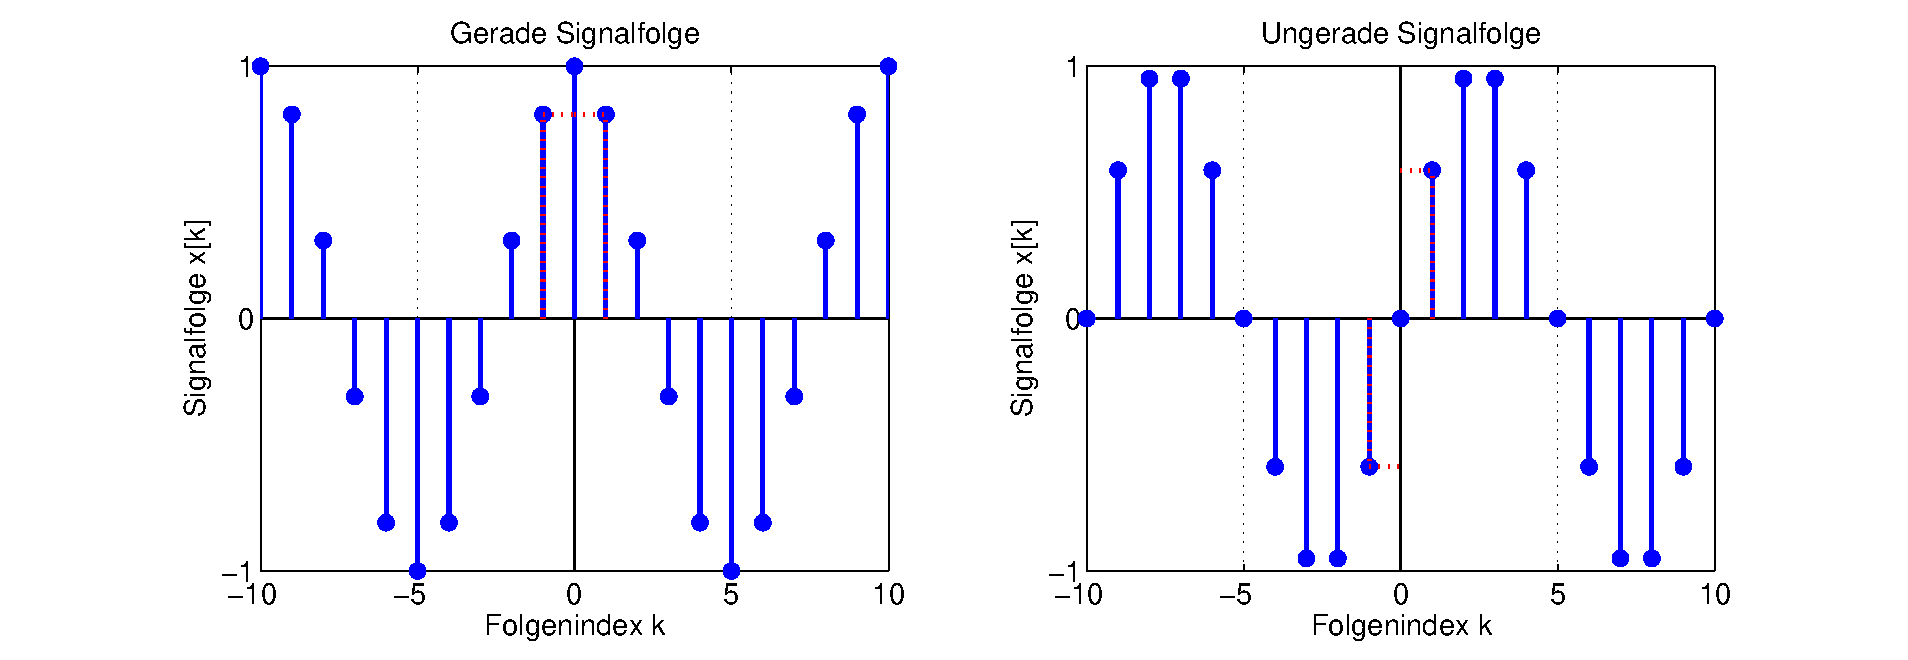
\includegraphics[width=1\textwidth]{Kapitel3/Bilder/image5}}
  \caption{Darstellung der Toleranzwerte eines Sensors}
  \label{fig:AuswertungDrucksensor}
\end{figure}

\noindent Anhand der Darstellung in Bild \ref{fig:AuswertungDrucksensor} wird unmittelbar deutlich, dass durch die Klassenbildung Information verloren gegangen ist, die Aufl\"{o}sung der Summenh\"{a}ufigkeit ist schlechter. Aus diesem Grund wird bei stetigen Merkmalstypen wenn m\"{o}glich eine Klassenbildung vermieden.

\subsubsection{Beschreibung ordinaler oder gruppierender Merkmalstypen}

\noindent Gruppierende oder ordinale Merkmale k\"{o}nnen nicht als Stabdiagramm dargestellt werden, da keine numerische Einteilung der Abszissenachse m\"{o}glich ist. Deshalb werden gruppierende oder ordinale Merkmale meist als Kreis- oder Balkendiagramm dargestellt. Ein Beispiel f\"{u}r einen gruppierenden Datensatz ist die Aufteilung einer Gesamtliefermenge von N = 10000 Teilen auf vier Zulieferer. In Tabelle \ref{tab:threefour} ist die Liefermenge der einzelnen Zulieferer aufgelistet.

\begin{table}[H]
\caption{Auswahl von Funktionen zur Signalverknüpfung}
\setlength{\fboxsep}{0pt}%
\colorbox{lightgray}{%
\arrayrulecolor{white}%
\begin{tabular}{| c | c | c |}
\hline
\parbox[c][0.5in][c]{2.2in}{\smallskip\centering\textbf{\fontfamily{phv}\selectfont{Zulieferer\\ Z}}} & 
\parbox[c][0.5in][c]{2.2in}{\smallskip\centering\textbf{\fontfamily{phv}\selectfont{Absolute\\ Liefermenge h$_{\mathbf{A}}$(Z)}}} &
\parbox[c][0.5in][c]{2.2in}{\smallskip\centering\textbf{\fontfamily{phv}\selectfont{Relative\\ Liefermenge h(Z)}}} \\ \hline

\parbox[c][0.3in][c]{2.2in}{\centering{\fontfamily{phv}\selectfont{A}}} &
\parbox[c][0.3in][c]{2.2in}{\centerline{4000}} &
\parbox[c][0.3in][c]{2.2in}{\centering{40 \%}} \\ \hline

\parbox[c][0.3in][c]{2.2in}{\centering{\fontfamily{phv}\selectfont{B}}} &
\parbox[c][0.3in][c]{2.2in}{\centerline{2000}} &
\parbox[c][0.3in][c]{2.2in}{\centering{20 \%}} \\ \hline

\parbox[c][0.3in][c]{2.2in}{\centering{\fontfamily{phv}\selectfont{C}}} &
\parbox[c][0.3in][c]{2.2in}{\centerline{3000}} &
\parbox[c][0.3in][c]{2.2in}{\centering{30 \%}} \\ \hline

\parbox[c][0.3in][c]{2.2in}{\centering{\fontfamily{phv}\selectfont{D}}} &
\parbox[c][0.3in][c]{2.2in}{\centerline{1000}} &
\parbox[c][0.3in][c]{2.2in}{\centering{10 \%}} \\ \hline

\end{tabular}%
}\bigskip
\label{tab:threefour}
\end{table}

\noindent In Bild \ref{fig:Zuliefererbewertung1} ist links die grafische Darstellung der relativen Liefermengen der einzelnen Zulieferer Z als Kreisdiagramm zu sehen. Jeder Teilsektor entspricht dabei einer relativen Liefermenge, die dem einzelnen Zulieferer zugeordnet werden kann. Die Fl\"{a}che der einzelnen Kreissektoren ist dabei proportional zu der relativen H\"{a}ufigkeit der Liefermenge h(Z). Der gesamte Kreis stellt die Summe aller Teilwerte dar, die Fl\"{a}che bei der Darstellung von relativen H\"{a}ufigkeiten ist damit 1. Gleiches gilt f\"{u}r die Darstellung der relativen Liefermenge h(Z) als Stapelbalkendiagramm, wie sie rechts in Bild \ref{fig:Zuliefererbewertung1} dargestellt ist.

\noindent 
\begin{figure}[H]
  \centerline{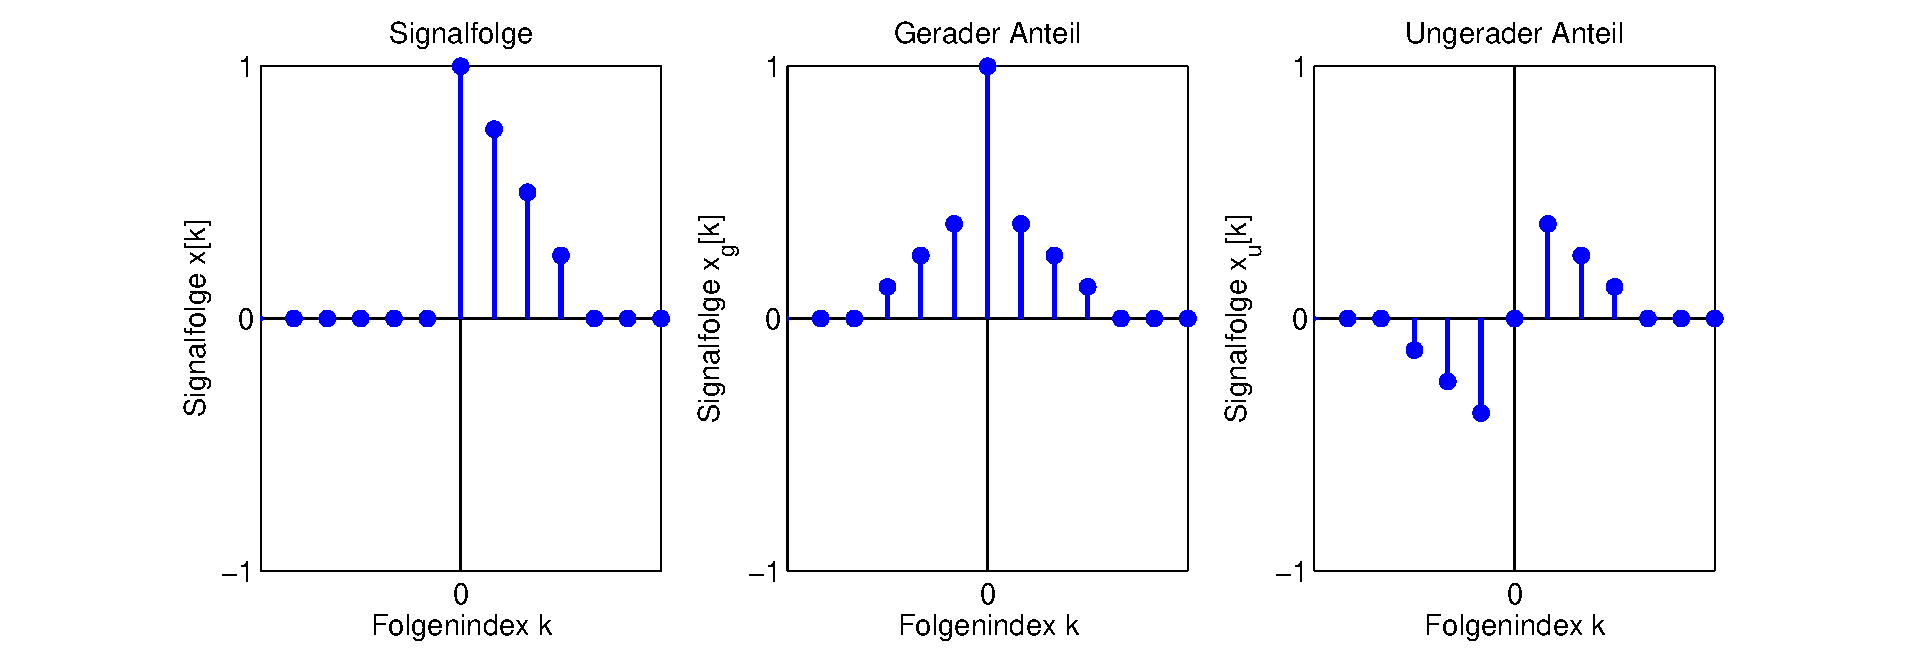
\includegraphics[width=1\textwidth]{Kapitel3/Bilder/image6}}
  \caption{Darstellung der relativen Liefermenge als Kreisdiagramm und als Stapelbalkendiagramm}
  \label{fig:Zuliefererbewertung1}
\end{figure}

\noindent Bei Darstellungen mithilfe von Kreis- oder Stapelbalkendiagrammen sollte darauf geachtet werden, dass der Kreis beziehungsweise der Balken nicht in zu viele Sektoren unterteilt wird, da sonst die \"{U}bersichtlichkeit des Diagrammes verloren geht. Es empfiehlt sich in diesem Fall, mehrere Sektoren zusammenzufassen. 

\noindent Ein Vergleich der einzelnen Zulieferer l\"{a}sst sich am besten mit einem einfachen Balkendiagramm erzielen. Dieses ist f\"{u}r die Werte aus Tabelle \ref{tab:threefour} in Bild \ref{fig:Zuliefererbewertung2} dargestellt.

\noindent 
\begin{figure}[H]
  \centerline{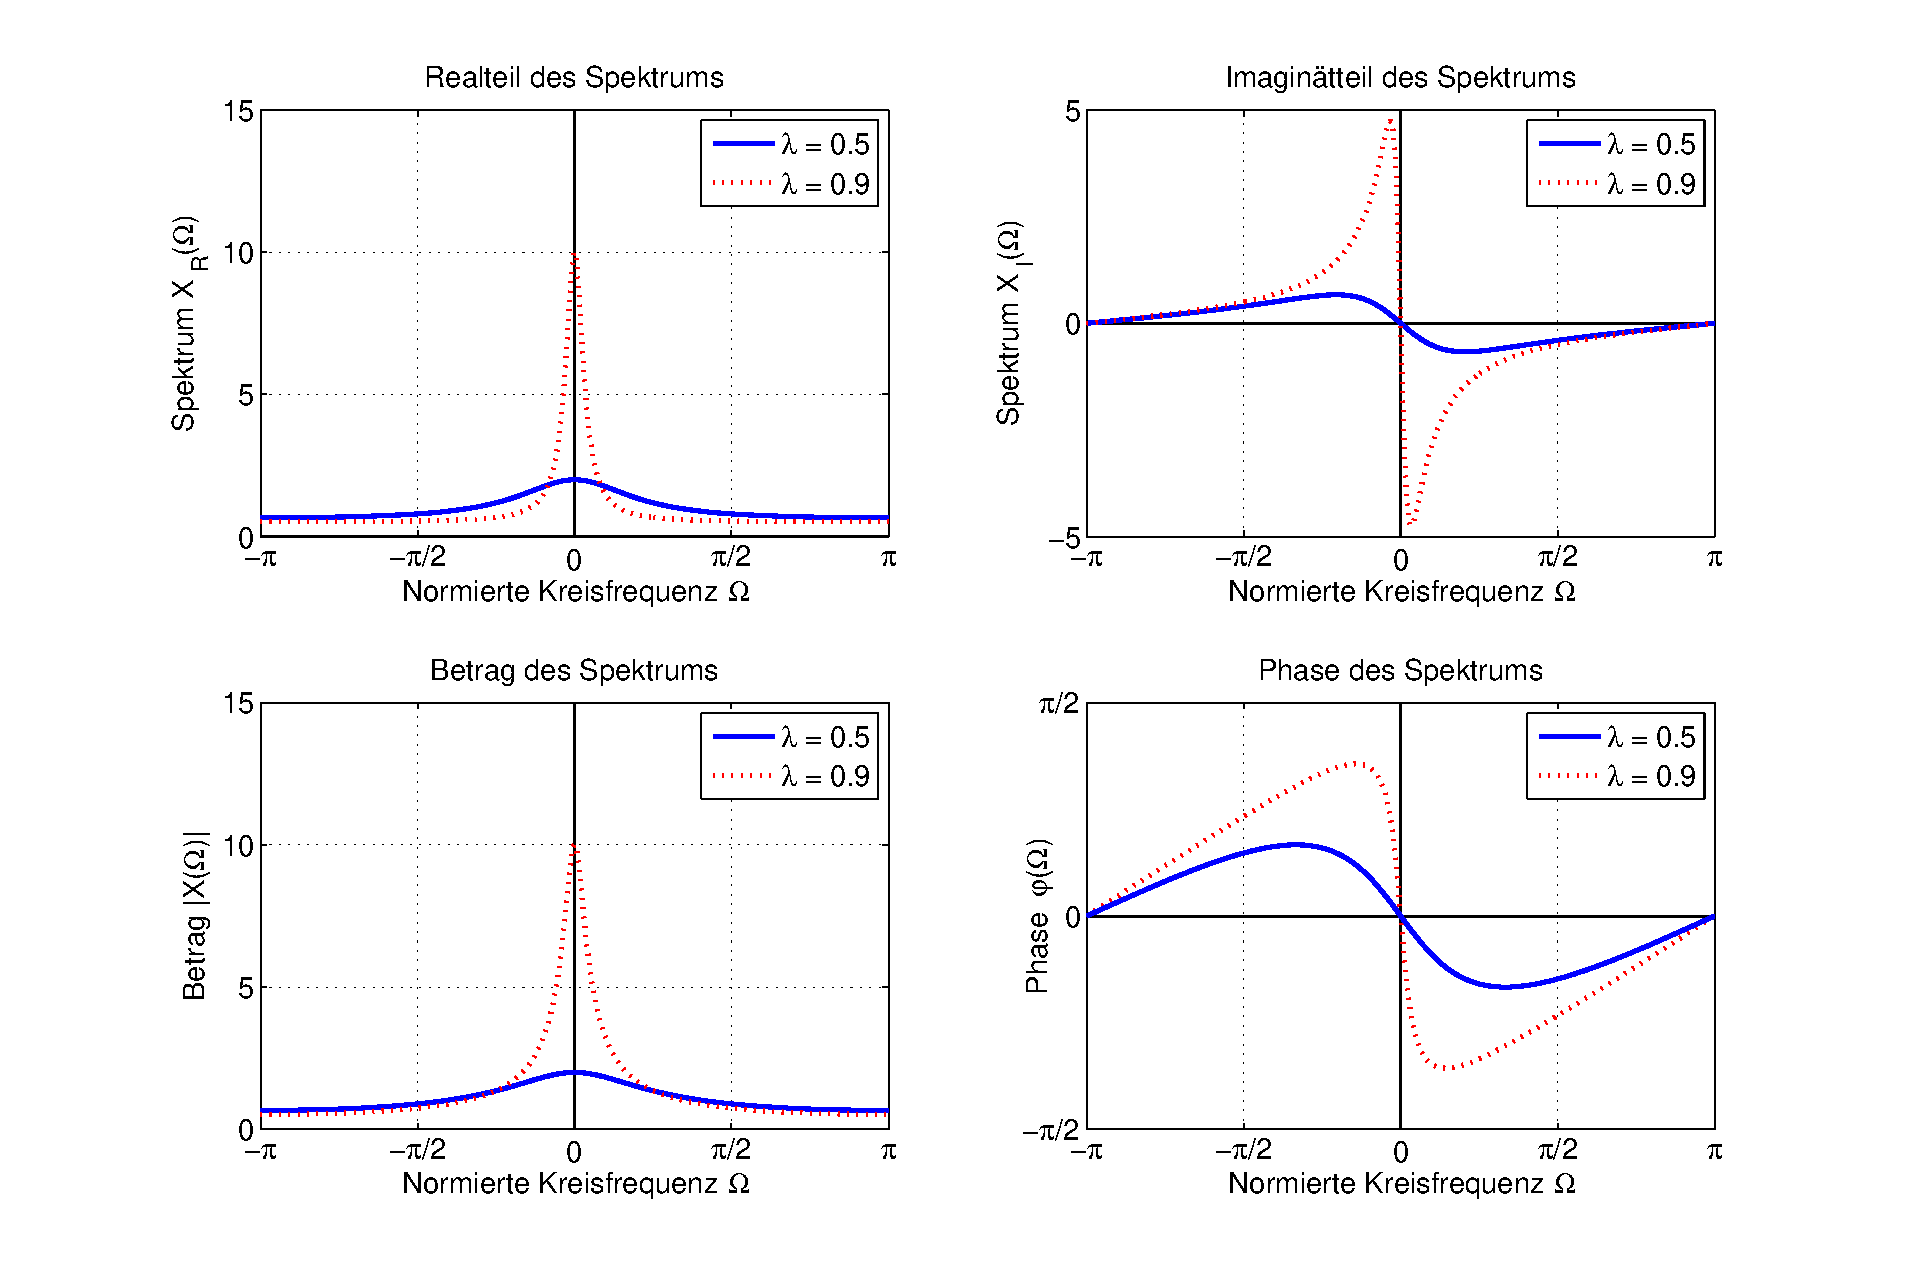
\includegraphics[width=0.5\textwidth]{Kapitel3/Bilder/image7}}
  \caption{Darstellung der relativen Liefermenge als Balkendiagramm}
  \label{fig:Zuliefererbewertung2}
\end{figure}

\noindent Bei dem Balkendiagramm in Bild \ref{fig:Zuliefererbewertung2} ist im Vergleich zu Bild \ref{fig:Zuliefererbewertung1} gut zu erkennen, dass Zulieferer A mit einem Lieferanteil von 40 \% das Vierfache von Zulieferer D liefert.

\clearpage

\subsubsection{Befehle zur Beschreibung von H\"{a}ufigkeiten in MATLAB}

\noindent Zur Berechnung und Darstellung von H\"{a}ufigkeitsverteilungen stehen in MATLAB diverse Funktionen zur Verf\"{u}gung. Die wichtigsten sind in Tabelle \ref{tab:threefive} zusammengefasst.

\begin{table}[H]
\setlength{\arrayrulewidth}{.1em}
\caption{Berechnung und Darstellung von H\"{a}ufigkeitsverteilungen in MATLAB}
\setlength{\fboxsep}{0pt}%
\colorbox{lightgray}{%
\arrayrulecolor{white}%
\begin{tabular}{| c | c |}
\hline
\parbox[c][0.3in][c]{3.3in}{\smallskip\centering\textbf{\fontfamily{phv}\selectfont{MATLAB Befehl}}} & 
\parbox[c][0.3in][c]{3.3in}{\smallskip\centering\textbf{\fontfamily{phv}\selectfont{Funktionsbeschreibung}}}\\ \hline

\parbox[c][0.3in][c]{3.3in}{\centering\fontfamily{phv}\selectfont{sort(x)}} & 
\parbox[c][0.3in][c]{3.3in}{\centering\fontfamily{phv}\selectfont{Sortiert die Werte des Vektors x nach der Gr\"{o}{\ss}e}}\\ \hline

\parbox[c][0.3in][c]{3.3in}{\centering\fontfamily{phv}\selectfont{cumsum(x)}} & 
\parbox[c][0.3in][c]{3.3in}{\centering\fontfamily{phv}\selectfont{Berechnet die kumulative Summe des Vektors x}}\\ \hline

\parbox[c][0.5in][c]{3.3in}{\centering\fontfamily{phv}\selectfont{hist(x)}} & 
\parbox[c][0.5in][c]{3.3in}{\centering\fontfamily{phv}\selectfont{Erzeugt ein Histogramm mit der absoluten H\"{a}ufigkeit von x}}\\ \hline

\parbox[c][0.3in][c]{3.3in}{\centering\fontfamily{phv}\selectfont{tabulate(x)}} & 
\parbox[c][0.3in][c]{3.3in}{\centering\fontfamily{phv}\selectfont{Erstellt eine H\"{a}ufigkeitstabelle aus x}}\\ \hline

\parbox[c][0.5in][c]{3.3in}{\centering\fontfamily{phv}\selectfont{bar(x)}} & 
\parbox[c][0.5in][c]{3.3in}{\centering\fontfamily{phv}\selectfont{Erzeugt ein Balkendiagramm ausx mit vertikaler Ausrichtung}}\\ \hline

\parbox[c][0.5in][c]{3.3in}{\centering\fontfamily{phv}\selectfont{barh(x)}} & 
\parbox[c][0.5in][c]{3.3in}{\centering\fontfamily{phv}\selectfont{Erzeugt ein Balkendiagramm ausX mit horizontaler Ausrichtung}}\\ \hline

\parbox[c][0.3in][c]{3.3in}{\centering\fontfamily{phv}\selectfont{pie(x)}} & 
\parbox[c][0.3in][c]{3.3in}{\centering\fontfamily{phv}\selectfont{Erzeugt ein Kreisdiagramm aus x}}\\ \hline

\end{tabular}%
}
\label{tab:threefive}
\end{table}

\subsubsection{Befehle zur Beschreibung von H\"{a}ufigkeiten in Python}

\noindent Zur Berechnung und Darstellung von H\"{a}ufigkeitsverteilungen stehen in Python diverse Funktionen zur Verf\"{u}gung. Die wichtigsten sind in Tabelle \ref{tab:threesix} zusammengefasst.

\begin{table}[H]
\setlength{\arrayrulewidth}{.1em}
\caption{Berechnung und Darstellung von H\"{a}ufigkeitsverteilungen in Python}
\setlength{\fboxsep}{0pt}%
\colorbox{lightgray}{%
\arrayrulecolor{white}%
\begin{tabular}{| c | c |}
\hline
\parbox[c][0.3in][c]{3.3in}{\smallskip\centering\textbf{\fontfamily{phv}\selectfont{Python Befehl}}} & 
\parbox[c][0.3in][c]{3.3in}{\smallskip\centering\textbf{\fontfamily{phv}\selectfont{Funktionsbeschreibung}}}\\ \hline

\parbox[c][0.3in][c]{3.3in}{\centering\fontfamily{phv}\selectfont{sorted}} & 
\parbox[c][0.3in][c]{3.3in}{\centering\fontfamily{phv}\selectfont{Sortiert die Werte des Vektors x nach der Gr\"{o}{\ss}e}}\\ \hline

\parbox[c][0.3in][c]{3.3in}{\centering\fontfamily{phv}\selectfont{numpy.cumsum}} & 
\parbox[c][0.3in][c]{3.3in}{\centering\fontfamily{phv}\selectfont{Berechnet die kumulative Summe des Vektors x}}\\ \hline

\parbox[c][0.5in][c]{3.3in}{\centering\fontfamily{phv}\selectfont{numpy.histogram}} & 
\parbox[c][0.5in][c]{3.3in}{\centering\fontfamily{phv}\selectfont{Erzeugt ein Histogramm mit der absoluten H\"{a}ufigkeit von x}}\\ \hline

\parbox[c][0.3in][c]{3.3in}{\centering\fontfamily{phv}\selectfont{count}} & 
\parbox[c][0.3in][c]{3.3in}{\centering\fontfamily{phv}\selectfont{Erstellt eine H\"{a}ufigkeitstabelle aus x}}\\ \hline

\parbox[c][0.5in][c]{3.3in}{\centering\fontfamily{phv}\selectfont{matplotlib.pyplot.bar}} & 
\parbox[c][0.5in][c]{3.3in}{\centering\fontfamily{phv}\selectfont{Erzeugt ein Balkendiagramm ausx mit vertikaler Ausrichtung}}\\ \hline

\parbox[c][0.5in][c]{3.3in}{\centering\fontfamily{phv}\selectfont{matplotlib.pyplot.barh}} & 
\parbox[c][0.5in][c]{3.3in}{\centering\fontfamily{phv}\selectfont{Erzeugt ein Balkendiagramm ausX mit horizontaler Ausrichtung}}\\ \hline

\parbox[c][0.3in][c]{3.3in}{\centering\fontfamily{phv}\selectfont{matplotlib.pyplot.pie}} & 
\parbox[c][0.3in][c]{3.3in}{\centering\fontfamily{phv}\selectfont{Erzeugt ein Kreisdiagramm aus x}}\\ \hline

\end{tabular}%
}
\label{tab:threesix}
\end{table}

\clearpage

\subsection{Kennwerte einer Stichprobe}

\noindent Jede Stichprobe wird mit ihrer H\"{a}ufigkeitsverteilung oder Summenh\"{a}ufigkeitsverteilung in allen Einzelheiten beschrieben. Gerade bei dem Vergleich gr\"{o}{\ss}erer Datenmengen sind diese H\"{a}ufigkeitsverteilungen aber unhandlich. Die Methoden der Statistik werden dazu verwendet, Stichproben \"{u}ber charakteristische Kenngr\"{o}{\ss}en oder Ma{\ss}zahlen abstrakt zu beschreiben. Dabei sind Kenngr\"{o}{\ss}en f\"{u}r die Lage, die Streuung und die Symmetrie einer Stichprobe zu unterscheiden. 

\subsubsection{Lagekennwerte einer Stichprobe}\label{threethreeone}

\noindent Lagekennwerte beschreiben die Lage des Zentrums einer Verteilung durch einen numerischen Wert.\bigskip

{\fontfamily{phv}\selectfont
\noindent\textbf{Arithmetischer Mittelwert einer Stichprobe}}\smallskip

\noindent Der arithmetische Mittelwert einer Stichprobe ist wohl die bekannteste Lagekenngr\"{o}{\ss}e. Er ist definiert als 

\begin{equation}\label{eq:threefifteen}
\bar{x}=\dfrac{x_{1} +{\rm \; ...\; }+x_{N} }{N} =\dfrac{1}{N} \cdot \sum _{n=1}^{N}x_{n}
\end{equation}

\noindent Liegen die Daten in Klassen mit ihren Klassenmitten $c_{n}$ vor, berechnet sich der arithmetische Mittelwert aus 

\begin{equation}\label{eq:threesixteen}
\bar{x}=\dfrac{c_{1} \cdot h_{A} (c_{1} )+{\rm \; ...\; }+c_{N} \cdot h_{A} (c_{N} )}{N} =\dfrac{1}{N} \cdot \sum _{n=1}^{N}(c_{n} \cdot h_{A} (c_{n})) =\sum _{n=1}^{N}(c_{n} \cdot h(c_{n}))
\end{equation}

Der arithmetische Mittelwert hat zwei wichtige Eigenschaften. Zum einen ist die Summe der Differenzen aller Werte von ihrem Mittelwert null. Diese Eigenschaft l\"{a}sst sich durch Zerlegen der Summe beweisen.

\begin{equation}\label{eq:threeseventeen}
\sum _{n=1}^{N}(x_{n} -\bar{x}) =\sum _{n=1}^{N}x_{n}  -\sum _{n=1}^{N}\bar{x} =\sum _{n=1}^{N}x_{n}  -N\cdot \bar{x}=N\cdot \bar{x}-N\cdot \bar{x}=0
\end{equation}

\noindent Zum anderen kann gezeigt werden, dass die Summe der Quadrate der Differenzen aller Werte von ihrem Mittelwert kleiner ist als die Summe der Quadrate der Differenzen aller Werte zu irgendeinem anderen Wert z. 

\begin{equation}\label{eq:threeeighteen}
\sum _{n=1}^{N}(x_{n} -\bar{x})^{2}  <\sum _{n=1}^{N}(x_{n} -z)^{2}
\end{equation}

\noindent Der arithmetische Mittelwert ist eine Kenngr\"{o}{\ss}e, die gerade bei kleinem Stichprobenumfang stark von einzelnen Ausrei{\ss}ern abh\"{a}ngig sein kann.

\clearpage

\noindent
\colorbox{lightgray}{%
\arrayrulecolor{white}%
\renewcommand\arraystretch{0.6}%
\begin{tabular}{ wl{16.5cm} }
{\fontfamily{phv}\selectfont
\noindent{Beispiel: Kapazit\"{a}tsmessung}}
\end{tabular}%
}\bigskip

\noindent Als Beispiel sind in Tabelle \ref{tab:threeseven} zwei Messreihen dargestellt, in denen jeweils N = 10 Kondensatoren mit einem nominalen Kapazit\"{a}tswert von C = 100 nF vermessen wurden. In der zweiten Messreihe wurde ein Messwert durch einen Ausrei{\ss}er ersetzt.

\begin{table}[H]
\setlength{\arrayrulewidth}{.1em}
\caption{Beispiel f\"{u}r eine Urliste: Messwerte von 100 Widerst\"{a}nden mit einem Sollwert von $R = 1 k \Omega $}
\setlength{\fboxsep}{0pt}%
\colorbox{lightgray}{%
\arrayrulecolor{white}%
\begin{tabular}{wc{0cm}  wl{0.9cm} | wc{1.3cm} | wc{1.3cm} | wc{1.3cm} | wc{1.3cm} | wc{1.3cm} | wc{1.3cm} | wc{1.3cm} | wc{1.3cm} | wc{1.3cm} }
\hline\xrowht{15pt}

& \multicolumn{10}{c}{\fontfamily{phv}\selectfont\textbf{Messreihe 1: Kapazit\"{a}tswerte C / nF}} \\ \hline \xrowht{15pt}

& 101 & 102 & 99 & 98 & 100 & 97 & 99 & 100 & 101 & 103\\ \hline\xrowht{15pt}

& \multicolumn{10}{c}{\fontfamily{phv}\selectfont\textbf{Messreihe 2: Kapazit\"{a}tswerte C / nF}} \\ \hline \xrowht{15pt}

& 101 & 153 & 99 & 98 & 100 & 97 & 99 & 100 & 101 & 103 \\ \hline

\end{tabular}%
}
\label{tab:threeseven}
\end{table}

\noindent Der arithmetische Mittelwert f\"{u}r Messreihe 1 ergibt sich aus 

\begin{equation}\label{eq:threenineteen}
\overline{C}_{1} =\dfrac{1}{N} \cdot \sum _{n=1}^{N}C_{n,1}  =\dfrac{101+102+...+103}{10} nF= 100 nF
\end{equation}

\noindent Wegen des Messfehlers in der zweiten Messreihe weicht der arithmetische Mittelwert stark von dem nominellen Wert ab. F\"{u}r Messreihe 2 ergibt sich der Mittelwert zu

\begin{equation}\label{eq:threetwenty}
\overline{C}_{2} =\dfrac{1}{N} \cdot \sum _{n=1}^{N}C_{n,2}  =\dfrac{101+153+...+103}{10} nF= 105.1 nF
\end{equation}

\noindent Das Beispiel best\"{a}tigt die Empfindlichkeit des arithmetischen Mittelwertes gegen\"{u}ber Ausrei{\ss}ern. Mit fallendem Stichprobenumfang steigt der Einfluss der Fehlmessung weiter an. \bigskip

{\fontfamily{phv}\selectfont
\noindent\textbf{Median einer Stichprobe}}\smallskip

\noindent Ein Lagema{\ss}, das weniger empfindlich auf Ausrei{\ss}er reagiert als der arithmetische Mittelwert, ist der Median. Der Median $x_{MED}$ ist der Wert, bei dem die H\"{a}lfte der Stichprobenwerte x gr\"{o}{\ss}er und die H\"{a}lfte der Stichprobenwerte x kleiner ist. 

\begin{equation}\label{eq:threetwentyone}
H(x_{MED})=0.5
\end{equation}

\noindent Bei ungeradem Stichprobenumfang n ist der Median $x_{MED}$ der mittlere Wert der nach Gr\"{o}{\ss}e geordneten Stichprobe. Bei geradem Stichprobenumfang ergibt sich der Median aus dem Mittelwert der beiden Stichprobenwerte, die in der Mitte der geordneten Stichprobe liegen.

\clearpage

\noindent
\colorbox{lightgray}{%
\arrayrulecolor{white}%
\renewcommand\arraystretch{0.6}%
\begin{tabular}{ wl{16.5cm} }
{\fontfamily{phv}\selectfont
\noindent{Beispiel: Kapazit\"{a}tsmessung}}
\end{tabular}%
}\bigskip

\noindent Zur Bestimmung des Medians f\"{u}r die Messreihen aus Tabelle \ref{tab:threeseven} m\"{u}ssen die Daten zun\"{a}chst sortiert werden.

\begin{table}[H]
\setlength{\arrayrulewidth}{.1em}
\caption{Beispiel f\"{u}r eine Urliste: Messwerte von 100 Widerst\"{a}nden mit einem Sollwert von $R = 1 k \Omega $}
\setlength{\fboxsep}{0pt}%
\colorbox{lightgray}{%
\arrayrulecolor{white}%
\begin{tabular}{wc{0cm}  wl{0.9cm} | wc{1.3cm} | wc{1.3cm} | wc{1.3cm} | wc{1.3cm} | wc{1.3cm} | wc{1.3cm} | wc{1.3cm} | wc{1.3cm} | wc{1.3cm} }
\hline\xrowht{15pt}

& \multicolumn{10}{c}{\fontfamily{phv}\selectfont\textbf{Messreihe 1: Kapazit\"{a}tswerte C / nF}} \\ \hline \xrowht{15pt}

& 97 & 98 & 99 & 99 & 100 & 100 & 101 & 101 & 102 & 103\\ \hline\xrowht{15pt}

& \multicolumn{10}{c}{\fontfamily{phv}\selectfont\textbf{Messreihe 2: Kapazit\"{a}tswerte C / nF}} \\ \hline \xrowht{15pt}

& 97 & 98 & 99 & 99 & 100 & 100 & 101 & 101 & 103 & 153 \\ \hline

\end{tabular}%
}
\label{tab:threeeight}
\end{table}

\noindent Aus den Messreihen 1 und 2 ergeben sich die beiden Mediane aus den arithmetischen Mittelwerten des f\"{u}nften und sechsten Elementes zu 

\begin{equation}\label{eq:threetwentytwo}
C_{MED,1} =\dfrac{C_{5,1} +C_{6,1} }{2} = 100 nF
\end{equation}

\noindent beziehungsweise

\begin{equation}\label{eq:threetwentythree}
C_{MED,2} =\dfrac{C_{5,2} +C_{6,2} }{2} = 100 nF
\end{equation}

\noindent Das Beispiel zeigt, dass der Median deutlich unempfindlicher auf Messausrei{\ss}er reagiert als der arithmetische Mittelwert, in diesem Beispiel bleibt er sogar konstant. F\"{u}r den Median ist zum Beispiel der Absolutwert des gr\"{o}{\ss}ten und des kleinsten Stichprobenwertes v\"{o}llig gleichg\"{u}ltig. Der Median wird deshalb als resistenter oder robuster Lagekennwert bezeichnet.\newline

\noindent Liegen die Daten in gruppierter Form mit konstanter Klassenbreite d vor, kann die relative Lage des Medians in der Klasse ber\"{u}cksichtigt werden. Dazu wird zwischen den benachbarten Klassenmitten $c_{n}$ ein linearer Zusammenhang zwischen der Summenh\"{a}ufigkeit H(x) und dem Merkmal x angenommen. Bild \ref{fig:MedianKlassen}
stellt diese Annahme grafisch dar.

\noindent 
\begin{figure}[H]
  \centerline{\includegraphics[width=0.5\textwidth]{Kapitel3/Bilder/image8}}
  \caption{Lineare Interpolation zwischen Summenh\"{a}ufigkeit H(x) und Merkmal x}
  \label{fig:MedianKlassen}
\end{figure}

\noindent Die Steigung der Geraden zwischen den bekannten Werten f\"{u}r die Klassenmitten ergibt sich aus 

\begin{equation}\label{eq:threetwentyfour}
m=\dfrac{H(c_{n})-H(c_{n-1})}{c_{n} -c_{n-1} } =\dfrac{h(c_{n})}{d}
\end{equation}

\noindent Daraus folgt f\"{u}r die Summenh\"{a}ufigkeit des Medians die Geradengleichung

\begin{equation}\label{eq:threetwentyfive}
H(x_{MED})=0.5=H(c_{n-1})+m\cdot (x_{MED} -c_{n-1} )=H(c_{n-1})+\dfrac{h(c_{n} )}{d} \cdot (x_{MED} -c_{n-1})
\end{equation}

\noindent Sie kann nach dem Median aufgel\"{o}st werden. Es ergibt sich 

\begin{equation}\label{eq:threetwentysix}
x_{MED} =c_{n-1} +\dfrac{d\cdot(0.5-H(c_{n-1}))}{h(c_{n})}
\end{equation}

\noindent
\colorbox{lightgray}{%
\arrayrulecolor{white}%
\renewcommand\arraystretch{0.6}%
\begin{tabular}{ wl{16.5cm} }
{\fontfamily{phv}\selectfont
\noindent{Beispiel: Widerstandsmessung}}
\end{tabular}%
}\bigskip

\noindent F\"{u}r das Beispiel aus Tabelle 3.3 ergibt sich damit als Median 

\begin{equation}\label{eq:threetwentyseven}
R_{MED} =985\Omega +\dfrac{1\Omega \cdot (0.5-0.23)}{0.32} = 985.84 \Omega
\end{equation}

\noindent Der Wert erreicht eine Aufl\"{o}sung, die unterhalb der Klassenbreite d liegt. Sowohl das arithmetische Mittel als auch der Median m\"{u}ssen bei diskreten Datentypen nicht mit einer m\"{o}glichen Auspr\"{a}gung $x_{n}$ \"{u}bereinstimmen. Liegt der Median genau auf der Grenze zweier Klassen, kann diese Rechnung nicht durchgef\"{u}hrt werden. In diesem Fall entspricht der Median der Grenze der beiden Klassen.\bigskip

{\fontfamily{phv}\selectfont
\noindent\textbf{Weitere Lagekennwerte von Stichproben}}\smallskip

\noindent Neben dem arithmetischen Mittelwert und dem Median sind zwei weitere Kennwerte gebr\"{a}uchlich. Bei Wachstumsprozessen wird das geometrische Mittel $x_{G}$ verwendet, das sich bei einem Stichprobenumfang N aus der N-ten Wurzel des Produktes der einzelnen Stichprobenwerte berechnet.

\begin{equation}\label{eq:threetwentyeight}
x_{G} =\sqrt[{N}]{x_{1} \cdot {\rm \; ...\; }\cdot x_{N} } =\sqrt[{N}]{\prod _{i=1}^{N}x_{n}}
\end{equation}

\noindent Der Modus ist der am h\"{a}ufigsten vorkommende Wert einer Stichprobe, also der Wert mit der gr\"{o}{\ss}ten absoluten oder relativen H\"{a}ufigkeit. Auf beide Kennwerte wird hier nicht weiter eingegangen.

\clearpage

{\fontfamily{phv}\selectfont
\noindent\textbf{Zusammenfassung der Lagekennwerte von Stichproben}}\smallskip

\noindent Zur besseren \"{U}bersicht fasst Tabelle \ref{tab:threenine} die Lagekennwerte einer Stichprobe zusammen.

\begin{table}[H]
\setlength{\arrayrulewidth}{.1em}
\caption{Lagekennwerte einer Stichprobe}
\setlength{\fboxsep}{0pt}%
\colorbox{lightgray}{%
\arrayrulecolor{white}%
\begin{tabular}{| wc{5.5cm} | wc{5.5cm} | wc{5.5cm} }
\xrowht{15pt}

{\fontfamily{phv}\selectfont\textbf{Lagekennwert}} & 
{\fontfamily{phv}\selectfont\textbf{Definition}} &
{\fontfamily{phv}\selectfont\textbf{Bemerkungen}}\\ \hline \xrowht{35pt}

{\fontfamily{phv}\selectfont{Mittelwert}} &
$\bar{x}=\dfrac{x_{1} +{\rm \; ...\; }+x_{N} }{N} =\dfrac{1}{N} \cdot \sum _{n=1}^{N}x_{n}$ &
\multirow{4}{5cm}{\centering\fontfamily{phv}\selectfont{Empfindlich gegen\"{u}ber Ausrei{\ss}ern}}\\ 
\cline{1-2}\xrowht{35pt}
{\fontfamily{phv}\selectfont{Mittelwert von Daten in Klassen}} & 
$\bar{x}=\sum _{n=1}^{N}\left(x_{n} \cdot h(c_{n} )\right)$ & \\ \hline \xrowht{20pt}

{\fontfamily{phv}\selectfont{Median}} &
$H\left(x_{MED} \right)=0.5$ &
\multirow{5}{5cm}{\centering\fontfamily{phv}\selectfont{Weniger empfindlich gegen\"{u}ber Ausrei{\ss}ern als der Mittelwert}}\\ 
\cline{1-2}\xrowht{45pt}
{\fontfamily{phv}\selectfont{Median von Daten in Klassen}} & 
$x_{MED} =c_{n-1} +\dfrac{d\cdot \left(0.5-H\left(c_{n-1} \right)\right)}{h\left(c_{n} \right)} $ & \\ \hline \xrowht{20pt}

{\fontfamily{phv}\selectfont{Geometrisches Mittel}} &
$x_{G} =\sqrt[{N}]{x_{1} \cdot {\rm \; ...\; }\cdot x_{N} } $ & \\ \hline \xrowht{20pt}

{\fontfamily{phv}\selectfont{Modus}} &
{\fontfamily{phv}\selectfont{häufigster Wert einer Stichprobe}} & \\ \hline 

\end{tabular}%
}\bigskip
\label{tab:threenine}
\end{table}

\noindent Da zur Berechnung der Lagekennwerte meist entsprechende Software verwendet wird, ent-fällt in vielen Fällen eine Einteilung der Daten in Klassen. MATLAB bietet einige Funktionen, mit denen die Lagekennwerte von Stichproben bestimmt werden können. Sie sind in Tabelle \ref{tab:threeten} aufgelistet.

\begin{table}[H]
\setlength{\arrayrulewidth}{.1em}
\caption{Berechnung der Lagekennwerte von Stichproben in MATLAB}
\setlength{\fboxsep}{0pt}%
\colorbox{lightgray}{%
\arrayrulecolor{white}%
\begin{tabular}{| c | c |}
\hline
\parbox[c][0.3in][c]{3.3in}{\smallskip\centering\textbf{\fontfamily{phv}\selectfont{Lagekennwert}}} & 
\parbox[c][0.3in][c]{3.3in}{\smallskip\centering\textbf{\fontfamily{phv}\selectfont{MATLAB-Befehl}}}\\ \hline

\parbox[c][0.3in][c]{3.3in}{\centering\fontfamily{phv}\selectfont{Mittelwert}} & 
\parbox[c][0.3in][c]{3.3in}{\centering\fontfamily{phv}\selectfont{mean(X)}}\\ \hline

\parbox[c][0.3in][c]{3.3in}{\centering\fontfamily{phv}\selectfont{Median}} & 
\parbox[c][0.3in][c]{3.3in}{\centering\fontfamily{phv}\selectfont{median(x)}}\\ \hline

\parbox[c][0.3in][c]{3.3in}{\centering\fontfamily{phv}\selectfont{Geometrisches Mittel }} & 
\parbox[c][0.3in][c]{3.3in}{\centering\fontfamily{phv}\selectfont{geomean(X)}}\\ \hline

\parbox[c][0.3in][c]{3.3in}{\centering\fontfamily{phv}\selectfont{Modus}} & 
\parbox[c][0.3in][c]{3.3in}{\centering\fontfamily{phv}\selectfont{mode(X)}}\\ \hline

\end{tabular}%
}
\label{tab:threeten}
\end{table}

\noindent Vergleichbare Befehle existieren in Python, sie sind in Tabelle \ref{tab:threeeleven} zusammengestellt.

\begin{table}[H]
\setlength{\arrayrulewidth}{.1em}
\caption{Berechnung der Lagekennwerte von Stichproben in Python}
\setlength{\fboxsep}{0pt}%
\colorbox{lightgray}{%
\arrayrulecolor{white}%
\begin{tabular}{| c | c |}
\hline
\parbox[c][0.3in][c]{3.3in}{\smallskip\centering\textbf{\fontfamily{phv}\selectfont{Lagekennwert}}} & 
\parbox[c][0.3in][c]{3.3in}{\smallskip\centering\textbf{\fontfamily{phv}\selectfont{MATLAB-Befehl}}}\\ \hline

\parbox[c][0.3in][c]{3.3in}{\centering\fontfamily{phv}\selectfont{Mittelwert}} & 
\parbox[c][0.3in][c]{3.3in}{\centering\fontfamily{phv}\selectfont{numpy.median}}\\ \hline

\parbox[c][0.3in][c]{3.3in}{\centering\fontfamily{phv}\selectfont{Median}} & 
\parbox[c][0.3in][c]{3.3in}{\centering\fontfamily{phv}\selectfont{numpy.mean}}\\ \hline

\parbox[c][0.3in][c]{3.3in}{\centering\fontfamily{phv}\selectfont{Geometrisches Mittel }} & 
\parbox[c][0.3in][c]{3.3in}{\centering\fontfamily{phv}\selectfont{scipy.stats.mstats.gmean}}\\ \hline

\parbox[c][0.3in][c]{3.3in}{\centering\fontfamily{phv}\selectfont{Modus}} & 
\parbox[c][0.3in][c]{3.3in}{\centering\fontfamily{phv}\selectfont{scipy.stats.mode}}\\ \hline

\end{tabular}%
}
\label{tab:threeeleven}
\end{table}

\subsubsection{Streuungskennwerte einer Stichprobe}\label{threethreetwo}

\noindent Der Mittelwert und der Median sind Kennwerte für die Lage einer Stichprobe. Für eine zu-sammenfassende Beschreibung ist es notwendig, zusätzlich die Streuung der Stichprobe zu charakterisieren. Dazu können Spannweite, Varianz und Quantile der Verteilung verwendet werden.\bigskip

{\fontfamily{phv}\selectfont
\noindent\textbf{Spannweite}}\smallskip

\noindent Die Spannweite oder Streu- beziehungsweise Variationsbreite einer Stichprobe ergibt sich aus der Differenz von gr\"{o}{\ss}tem und kleinstem Stichprobenwert. 

\begin{equation}\label{eq:threetwentynine}
\Delta x=x_{MAX} -x_{MIN}
\end{equation}

\noindent
\colorbox{lightgray}{%
\arrayrulecolor{white}%
\renewcommand\arraystretch{0.6}%
\begin{tabular}{ wl{16.5cm} }
{\fontfamily{phv}\selectfont
\noindent{Beispiel: Kapazit\"{a}tsmessung}}
\end{tabular}%
}\bigskip

\noindent F\"{u}r die Messreihen 1 und 2 aus Tabelle \ref{tab:threeseven} ergeben sich die beiden Spannweiten zu 

\begin{equation}\label{eq:threethirty}
\Delta C_{1} = 103 nF-97 nF=6 nF
\end{equation}

\noindent beziehungsweise 

\begin{equation}\label{eq:threethirtyone}
\Delta C_{2} = 153 nF - 97 nF = 56 nF
\end{equation}

\noindent Die Spannweite reagiert offensichtlich extrem auf Ausrei{\ss}er und besitzt damit bez\"{u}glich der Streuung aller Stichprobenwerte nur eine geringe Aussagekraft.\bigskip

{\fontfamily{phv}\selectfont
\noindent\textbf{Varianz und Standardabweichung}}

\noindent Die Varianz betrachtet die Streuung aller Stichprobenwerte um den Mittelwert. Die Summe der einzelnen Abweichungen heben sich auf.

\begin{equation}\label{eq:threethirtytwo}
\sum _{n=1}^{N}(x_{n} -\bar{x})= \sum _{n=1}^{N}x_{n} -N\cdot \bar{x}= 0
\end{equation}

\noindent Der Mittelwert kann deshalb nicht zur Bewertung der Streuung herangezogen werden. Eine bessere M\"{o}glichkeit zur Bestimmung der Streuung einer Stichprobe ergibt sich aus der Summe der quadrierten Abweichungen. Durch das Quadrieren werden alle Elemente der Summe positiv und k\"{o}nnen sich nicht mehr gegenseitig kompensieren. Es ergibt sich die Varianz $s^{2}$, die definiert ist als

\begin{equation}\label{eq:threethirtythree}
s^{2} =\dfrac{1}{N-1} \cdot \sum _{n=1}^{N}\left(x_{n} -\bar{x}\right)^{2}
\end{equation}

\noindent F\"{u}r eine manuelle Berechnung kann Gleichung \eqref{eq:threethirtythree} mit der binomischen Formel umgeformt werden zu

\begin{equation}\label{eq:threethirtyfour}
\begin{split}
s^{2}  & = \dfrac{1}{N-1} \cdot \sum _{n=1}^{N}(x_{n} -\bar{x})^{2}  =\dfrac{1}{N-1} \cdot \sum _{n=1}^{N}(x_{n}^{2} -2\cdot x_{n} \cdot \bar{x}+\bar{x}^{2} ) \\ 
& = \dfrac{1}{N-1} \cdot \left(\sum _{n=1}^{N} x^{2}_{n} - 2\cdot N \cdot \bar{x}^{2} + N\cdot \bar{x}^{2} \right) =  \dfrac{1}{N-1} \cdot  \left(\sum _{n=1}^{N} x^{2}_{n} -   N\cdot \bar{x}^{2} \right)
\end{split}
\end{equation}

\noindent Im Gegensatz zu dem Mittelwert wird bei der Varianz nicht durch die Anzahl N der Stichprobenwerte, sondern durch den Wert (N -- 1) geteilt. Mathematisch ergibt sich die Division durch den Wert (N -- 1) dadurch, dass bei der Bildung der Varianz die Differenzen zum Mittelwert ausgewertet werden. Der Mittelwert wird bereits mit diesen Daten berechnet, sodass ein Summand in Gleichung \eqref{eq:threethirtytwo} sich aus den \"{u}brigen (N -- 1) Werten ergibt. Es sind also nur (N -- 1) Summanden unabh\"{a}ngig oder frei. Es geht ein sogenannter Freiheitsgrad verloren, sodass die Division durch den Wert (N -- 1) gerechtfertigt ist. \bigskip

\noindent
\colorbox{lightgray}{%
\arrayrulecolor{white}%
\renewcommand\arraystretch{0.6}%
\begin{tabular}{ wl{16.5cm} }
{\fontfamily{phv}\selectfont
\noindent{Beispiel: Kapazit\"{a}tsmessung}}
\end{tabular}%
}\bigskip

\noindent F\"{u}r die Messreihen 1 und 2 aus Tabelle \ref{tab:threeseven} ergeben sich die beiden Varianzen zu 

\begin{equation}\label{eq:threethirtyfive}
s_{C1}^{2} = 3.33 n{F}^{2}
\end{equation}

\noindent beziehungsweise 

\begin{equation}\label{eq:threethirtysix}
s_{C2}^{2} = 286.1 n{F}^{2}
\end{equation}

\noindent Die Varianz ist ein Ma{\ss} f\"{u}r die Streuung, der physikalische Gehalt der Gr\"{o}{\ss}e ist aber unanschaulich. Aus diesem Grund wird f\"{u}r die Kennzeichnung einer Streuung oft die Standardabweichung verwendet. Die Standardabweichung s ergibt sich aus der positiven Quadratwurzel der Varianz $s^{2}$ und berechnet sich aus 

\begin{equation}\label{eq:threethirtyseven}
s=\sqrt{\dfrac{1}{N-1} \cdot \sum _{n=1}^{N}(x_{n} -\bar{x})^{2}}
\end{equation}

\noindent Die Standardabweichung hat dieselbe physikalische Dimension wie die Stichprobenwerte x und eignet sich damit gut f\"{u}r eine anschauliche Interpretation.\bigskip

\noindent
\colorbox{lightgray}{%
\arrayrulecolor{white}%
\renewcommand\arraystretch{0.6}%
\begin{tabular}{ wl{16.5cm} }
{\fontfamily{phv}\selectfont
\noindent{Beispiel: Kapazit\"{a}tsmessung}}
\end{tabular}%
}\bigskip

\noindent F\"{u}r die Messreihen 1 und 2 aus Tabelle \ref{tab:threeseven} ergeben sich die beiden Varianzen zu 

\begin{equation}\label{eq:threethirtyeight}
s_{C1}^{2} = 1.825 nF
\end{equation}

\noindent beziehungsweise 

\begin{equation}\label{eq:threethirtynine}
s_{C2}^{2} = 16.915 nF
\end{equation} 

\noindent Liegt die Stichprobe in Klassen vor, ergibt sich die Varianz aus 

\begin{equation}\label{eq:threefourty}
s^{2} =\dfrac{1}{N-1} \cdot \sum _{n=1}^{N}\left(h_{A} (c_{n})\cdot (c_{n} -\bar{x})^{2} \right)
\end{equation} 

\noindent und die Standardabweichung berechnet sich entsprechend zu

\begin{equation}\label{eq:threefourtyone}
s=\sqrt{\dfrac{1}{N-1} \cdot \sum _{n=1}^{N}\left(h_{A} (c_{n})\cdot (c_{n} -\bar{x})^{2} \right)}
\end{equation} 

{\fontfamily{phv}\selectfont
\noindent\textbf{Quantilabst\"{a}nde einer Stichprobe}}

\noindent Auch wenn die Empfindlichkeit der Varianz gegen\"{u}ber Ausrei{\ss}ern kleiner ist als die der Spannweite einer Stichprobe, reagiert die Standardabweichung auf Ausrei{\ss}er \"{a}hnlich stark wie der arithmetische Mittelwert. Aus diesem Grund werden Streuungskenngr\"{o}{\ss}en definiert, die sich an der Definition des Medians orientieren und als Quantile bezeichnet werden. Das P-Quantil $x_{P}$ einer Verteilung trennt die Daten so in zwei Teile, dass ein Anteil P unterhalb des Quantils liegt und ein Anteil (1 -- P) \"{u}ber dem Quantil liegt. 

\begin{equation}\label{eq:threefourtytwo}
H(x_{P})=P
\end{equation} 

\noindent Der Median entspricht dem 50\%-Quantil. Werden die Quantile die Stichprobe in vier Intervalle teilen, werden Sie als Quartile bezeichnet. Die Quartile eine Stichprobe lassen sich \"{a}hnlich wie der Median einer Stichprobe bestimmen. Auch die Rechenregeln f\"{u}r in Klassen eingeteilte Daten mit konstanter Klassenbreite d gelten sinngem\"{a}{\ss}, sodass die Quartile bestimmt werden durch

\begin{equation}\label{eq:threefourtythree}
x_{0.25} =c_{n-1} +\dfrac{d\cdot (0.25-H(c_{n-1}))}{h(c_{n})}
\end{equation} 

\begin{equation}\label{eq:threefourtyfour}
x_{0.75} =c_{n-1} +\dfrac{d\cdot (0.75-H(c_{n-1}))}{h(c_{n})}
\end{equation} 

\noindent Dar\"{u}ber hinaus ist eine grafische Bestimmung der Quartile aus der Summenh\"{a}ufigkeit m\"{o}glich. 

\noindent Der Abstand zwischen dem 75\%- und dem 25\%-Quartil wird als Interquartilabstand (inter quartile range) IQR bezeichnet. 

\begin{equation}\label{eq:threefourtyfive}
IQR=x_{0.75} -x_{0.25}
\end{equation} 

\noindent Der Interquartilabstand ist unempfindlich gegen Ausrei{\ss}er, weil er von der absoluten Lage der Stichprobenwerte, die am Rand der Verteilung liegen, unabh\"{a}ngig ist.

\clearpage

\noindent
\colorbox{lightgray}{%
\arrayrulecolor{white}%
\renewcommand\arraystretch{0.6}%
\begin{tabular}{ wl{16.5cm} }
{\fontfamily{phv}\selectfont
\noindent{Beispiel: Widerstandsmessung}}
\end{tabular}%
}\bigskip

\noindent Die Berechnung wird am Beispiel der Widerstandsmessung veranschaulicht. Bild \ref{fig:SummenhQuantileStichprobeWiderstand} zeigt die Summenh\"{a}ufigkeit der Stichprobe aus Tabelle 3.1 sowie die 25\%-, 50\%- und 75\%-Quantile der Stichprobe. 

\noindent 
\begin{figure}[H]
  \centerline{\includegraphics[width=0.5\textwidth]{Kapitel3/Bilder/image8}}
  \caption{Darstellung der Summenh\"{a}ufigkeit f\"{u}r die Stichprobe in Tabelle \ref{tab:threethree} mit Quartilen }
  \label{fig:SummenhQuantileStichprobeWiderstand}
\end{figure}

\noindent F\"{u}r die Daten in Tabelle \ref{tab:threethree} ergeben sich das 25\%- und 75\%-Quartil zu 

\begin{equation}\label{eq:threefourtysix}
R_{0.25} =985 \Omega +\dfrac{1 \Omega \cdot (0.25-0.23)}{0.32} = 985.06 \Omega
\end{equation} 

\begin{equation}\label{eq:threefourtyseven}
R_{0.75} =987 \Omega +\dfrac{1 \Omega \cdot (0.75-0.72)}{0.15} = 987.20 \Omega
\end{equation} 

\noindent Damit errechnet sich der Inter-Quartil-Range zu

\begin{equation}\label{eq:threefourtyeight}
IQR=R_{0.75} -R_{0.25} = 987.20 \Omega - 985.06 \Omega =2.14 \Omega 
\end{equation} 

\clearpage

{\fontfamily{phv}\selectfont
\noindent\textbf{Zusammenfassung der Streuungskennwerte von Stichproben}}

\noindent Zur besseren \"{U}bersicht fasst Tabelle \ref{tab:threetwelve} die Streuungskennwerte einer Stichprobe zusammen.

\begin{table}[H]
\setlength{\arrayrulewidth}{.1em}
\caption{Berechnung der Lagekennwerte von Stichproben in Python}
\setlength{\fboxsep}{0pt}%
\colorbox{lightgray}{%
\arrayrulecolor{white}%
\begin{tabular}{| wc{5.5cm} | wc{5.5cm} | wc{13em} }
\xrowht{15pt}

{\fontfamily{phv}\selectfont\textbf{Streuungskennwert}} & 
{\fontfamily{phv}\selectfont\textbf{Definition}} &
{\fontfamily{phv}\selectfont\textbf{Bemerkungen}}\\ \hline \xrowht{20pt}

\multirow{3}{*}{\fontfamily{phv}\selectfont{Spannweite}} &
\multirow{3}{*}{$\Delta x=x_{MAX} -x_{MIN} $} &
{\fontfamily{phv}\selectfont{Extrem empfindlich}} \\ \xrowht{20pt}
& & {\fontfamily{phv}\selectfont{gegenüber Ausreißern}}\\ \hline \xrowht{35pt}

{\fontfamily{phv}\selectfont{Varianz}} &
$s^{2} =\dfrac{1}{N-1} \cdot \sum _{n=1}^{N}(x_{n} -\bar{x})^{2}$ &
\multirow{5}{5cm}{\centering\fontfamily{phv}\selectfont{Empfindlich gegen\"{u}ber Ausrei{\ss}ern}}\\ \cline{1-2}\xrowht{15.5pt}
\fontfamily{phv}\selectfont{Varianz in Klassen} & \multirow{3}{*}{$s^{2} =\dfrac{1}{N-1} \cdot \sum _{n=1}^{N}\left(h_{A} (c_{n})\cdot (c_{n} -\bar{x}\right)^{2})$}&\\ \xrowht{15.5pt}
\fontfamily{phv}\selectfont{eingeteilter Daten} & & \\ \hline \xrowht{45pt}

{\fontfamily{phv}\selectfont{Standardabweichung}} &
$s=\sqrt{\dfrac{1}{N-1} \cdot \sum _{n=1}^{N}(x_{n} -\bar{x})^{2}}$ &
\multirow{5}{5cm}{\centering\fontfamily{phv}\selectfont{ Vergleichbar zur Varianz, aber in Einheiten der Zielgr\"{o}{\ss}e x}}\\ 
\cline{1-2}\xrowht{22.5pt}
\fontfamily{phv}\selectfont{Standardabweichungin Klassen} & \multirow{3}{*}{$s=\sqrt{\dfrac{1}{N-1} \cdot \sum _{n=1}^{N}\left(h_{A} \left(c_{n} \right)\cdot \left(c_{n} -\bar{x}\right)^{2} \right)}$}&\\ \xrowht{22.5pt}
\fontfamily{phv}\selectfont{eingeteilter Daten} & & \\ \hline\xrowht{20pt}

{\fontfamily{phv}\selectfont{P-Quantil}} &
$H\left(x_{P} \right)=P$ & \\ \hline \xrowht{15pt}

\fontfamily{phv}\selectfont{P-Quantilin Klassen} & \multirow{3}{*}{$x_{P} =c_{n-1} +\dfrac{d\cdot \left(P-H\left(c_{n-1} \right)\right)}{h\left(c_{n} \right)} $}&\\ \xrowht{15pt}
\fontfamily{phv}\selectfont{eingeteilter Daten} & & \\ \hline \xrowht{20pt}

{\fontfamily{phv}\selectfont{Interquartilabstand}} &
$IQR=x_{0.75} -x_{0.25} $ & 
{\fontfamily{phv}\selectfont{Robuster Streuungskennwert}} \\ \hline 

\end{tabular}%
}\bigskip
\label{tab:threetwelve}
\end{table}

\noindent Gerade bei gr\"{o}{\ss}eren Stichprobenumf\"{a}ngen ist es aufwendig, die Streuungskennwerte manuell zu berechnen. Daher wird zur Auswertung meist entsprechende Software herangezogen. Die Befehle zur Berechnung der Streuungskenngr\"{o}{\ss}en mit MATLAB sind in Tabelle \ref{tab:threethirteen} zusammengefasst.

\begin{table}[H]
\setlength{\arrayrulewidth}{.1em}
\caption{Berechnung der Streuungskennwerte von Stichproben in MATLAB}
\setlength{\fboxsep}{0pt}%
\colorbox{lightgray}{%
\arrayrulecolor{white}%
\begin{tabular}{| c | c |}
\hline
\parbox[c][0.3in][c]{3.3in}{\smallskip\centering\textbf{\fontfamily{phv}\selectfont{Streuungskennwert}}} & 
\parbox[c][0.3in][c]{3.3in}{\smallskip\centering\textbf{\fontfamily{phv}\selectfont{MATLAB-Befehl}}}\\ \hline

\parbox[c][0.3in][c]{3.3in}{\centering\fontfamily{phv}\selectfont{Spannweite}} & 
\parbox[c][0.3in][c]{3.3in}{\centering\fontfamily{phv}\selectfont{range(x) oder max(x)-min(x)}}\\ \hline

\parbox[c][0.3in][c]{3.3in}{\centering\fontfamily{phv}\selectfont{Varianz}} & 
\parbox[c][0.3in][c]{3.3in}{\centering\fontfamily{phv}\selectfont{var(x)}}\\ \hline

\parbox[c][0.3in][c]{3.3in}{\centering\fontfamily{phv}\selectfont{Standardabweichung}} & 
\parbox[c][0.3in][c]{3.3in}{\centering\fontfamily{phv}\selectfont{std(x)}}\\ \hline

\parbox[c][0.3in][c]{3.3in}{\centering\fontfamily{phv}\selectfont{p-Quantil}} & 
\parbox[c][0.3in][c]{3.3in}{\centering\fontfamily{phv}\selectfont{quantile(x,p)}}\\ \hline

\parbox[c][0.3in][c]{3.3in}{\centering\fontfamily{phv}\selectfont{Interquartilabstand}} & 
\parbox[c][0.3in][c]{3.3in}{\centering\fontfamily{phv}\selectfont{iqr(x)}}\\ \hline

\end{tabular}%
}
\label{tab:threethirteen}
\end{table}

\clearpage

\noindent Vergleichbare Befehle existieren in Python, sie sind in Tabelle \ref{tab:threefourteen} zusammengestellt.

\begin{table}[H]
\setlength{\arrayrulewidth}{.1em}
\caption{Berechnung der Streuungskennwerte von Stichproben in Python}
\setlength{\fboxsep}{0pt}%
\colorbox{lightgray}{%
\arrayrulecolor{white}%
\begin{tabular}{| c | c |}
\hline
\parbox[c][0.3in][c]{3.3in}{\smallskip\centering\textbf{\fontfamily{phv}\selectfont{Streuungskennwert}}} & 
\parbox[c][0.3in][c]{3.3in}{\smallskip\centering\textbf{\fontfamily{phv}\selectfont{Python-Befehl}}}\\ \hline

\parbox[c][0.3in][c]{3.3in}{\centering\fontfamily{phv}\selectfont{Spannweite}} & 
\parbox[c][0.3in][c]{3.3in}{\centering\fontfamily{phv}\selectfont{max - min}}\\ \hline

\parbox[c][0.3in][c]{3.3in}{\centering\fontfamily{phv}\selectfont{Varianz}} & 
\parbox[c][0.3in][c]{3.3in}{\centering\fontfamily{phv}\selectfont{numpy.var}}\\ \hline

\parbox[c][0.3in][c]{3.3in}{\centering\fontfamily{phv}\selectfont{Standardabweichung}} & 
\parbox[c][0.3in][c]{3.3in}{\centering\fontfamily{phv}\selectfont{numpy.std}}\\ \hline

\parbox[c][0.3in][c]{3.3in}{\centering\fontfamily{phv}\selectfont{p-Quantil}} & 
\parbox[c][0.3in][c]{3.3in}{\centering\fontfamily{phv}\selectfont{numpy.quantile}}\\ \hline

\parbox[c][0.3in][c]{3.3in}{\centering\fontfamily{phv}\selectfont{Interquartilabstand}} & 
\parbox[c][0.3in][c]{3.3in}{\centering\fontfamily{phv}\selectfont{numpy.quantile}}\\ \hline

\end{tabular}%
}
\label{tab:threefourteen}
\end{table}


\subsubsection{Schiefe oder Symmetrie einer Stichprobe}

\noindent Neben der Lage und Streuung einer Verteilung kann die Schiefe einer Verteilung angegeben werden. Die Schiefe ist ein Ma{\ss} f\"{u}r die Symmetrie der Verteilung zum Mittelwert. 

{\fontfamily{phv}\selectfont
\noindent\textbf{Definition von Schiefe und Symmetrie einer Stichprobe}}

\noindent Eine Stichprobe wird als symmetrisch bezeichnet, wenn es eine Symmetrieachse gibt, zu der die rechte und linke Seite der Verteilung ann\"{a}hernd zueinander spiegelbildlich sind. Exakte Symmetrie ist bei empirischen Verteilungen selten gegeben. Ein Beispiel f\"{u}r eine symmetrische Verteilung ist in Bild \ref{fig:DefinitionSchiefe} Mitte gegeben. Eine unsymmetrische Verteilung wird als schiefe Verteilung bezeichnet. Eine Verteilung hei{\ss}t rechtsschief, wenn der \"{u}berwiegende Teil der Daten linksseitig konzentriert ist. Dann f\"{a}llt die Verteilung wie die linke Grafik in Bild \ref{fig:DefinitionSchiefe} nach links deutlich steiler ab als nach rechts. Entsprechend hei{\ss}t eine Verteilung linksschief, wenn wie in der Verteilung der rechten Grafik in Bild \ref{fig:DefinitionSchiefe} der \"{u}berwiegende Teil der Daten rechtsseitig konzentriert ist und die Verteilung nach rechts deutlich steiler abf\"{a}llt.

\noindent 
\begin{figure}[H]
  \centerline{\includegraphics[width=1\textwidth]{Kapitel3/Bilder/image10}}
  \caption{Darstellung von Stichprobenverteilungen mit gleichem Mittelwert und unterschiedlicher Schiefe}
  \label{fig:DefinitionSchiefe}
\end{figure}

\noindent Die Schiefe kann mit zwei unterschiedlichen Kenngr\"{o}{\ss}en charakterisiert werden, dem Momentenkoeffizient und dem Quantilkoeffizient der Schiefe.

\clearpage

{\fontfamily{phv}\selectfont
\noindent\textbf{Momentenkoeffizient der Schiefe}}

\noindent In Analogie an die Varianz $s^{2}$ wird ein Momentenkoeffizient der Schiefe definiert.

\begin{equation}\label{eq:threefourtynine}
g_{M} =\dfrac{N}{(N-1)\cdot (N-2)} \cdot \sum _{n=1}^{N}(\dfrac{x_{n} -\bar{x}}{s} ) ^{3} 
\end{equation} 

\noindent Durch die dritte Potenz der Abweichung der Stichprobenwerte vom Mittelwert bleiben im Vergleich zur Standardabweichung die Vorzeichen bei den Abweichungen erhalten. Bei rechtsschiefen Verteilungen \"{u}berwiegen positive Abweichungen, sodass der Momentenkoeffizient $g_{M}$ positiv wird. Bei linksschiefen Verteilungen weist er entsprechend negative Werte auf. Wegen der Division durch die dritte Potenz der Standardabweichung ist der Momentenkoeffizient der Schiefe dimensionslos und unabh\"{a}ngig von der Messgr\"{o}{\ss}e. F\"{u}r den Fall von in Klassen aufgeteilten Daten errechnet sich der Momentenkoeffizient der Schiefe aus

\begin{equation}\label{eq:threefifty}
g_{M} =\dfrac{\dfrac{1}{N} \cdot \sum _{n=1}^{N}\left(h_{a} (c_{n} )\cdot (c_{n} -\bar{x})^{3} \right) }{s^{3} }
\end{equation} 

\noindent Positive Werte f\"{u}r den Momentenkoeffizienten der Schiefe weisen auf rechtsschiefe Verteilungen, negative Werte weisen auf linksschiefe Verteilungen hin. Ist der Momentenkoeffizient der Schiefe nahe null, handelt es sich um eine symmetrische Verteilung.

\begin{table}[H]
\setlength{\arrayrulewidth}{.1em}
\caption{Bewertung des Momentenkoeffizienten der Schiefe $g_{M}$}
\setlength{\fboxsep}{0pt}%
\colorbox{lightgray}{%
\arrayrulecolor{white}%
\begin{tabular}{| c | c |}
\hline
\parbox[c][0.3in][c]{3.3in}{\smallskip\centering\textbf{\fontfamily{phv}\selectfont{Kennwert}}} & 
\parbox[c][0.3in][c]{3.3in}{\smallskip\centering\textbf{\fontfamily{phv}\selectfont{Symmetrieeigenschaft}}}\\ \hline

\parbox[c][0.3in][c]{3.3in}{\centering\fontfamily{phv}\selectfont{$g_{M}\mathrm{>} 0$}} & 
\parbox[c][0.3in][c]{3.3in}{\centering\fontfamily{phv}\selectfont{tRechtsschiefe Verteilung}}\\ \hline

\parbox[c][0.3in][c]{3.3in}{\centering\fontfamily{phv}\selectfont{$g_{M} = 0$}} & 
\parbox[c][0.3in][c]{3.3in}{\centering\fontfamily{phv}\selectfont{Symmetrische Verteilung}}\\ \hline

\parbox[c][0.3in][c]{3.3in}{\centering\fontfamily{phv}\selectfont{$g_{M} \mathrm{<} 0$}} & 
\parbox[c][0.3in][c]{3.3in}{\centering\fontfamily{phv}\selectfont{Linksschiefe Verteilung}}\\ \hline

\end{tabular}%
}
\label{tab:threefifteen}
\end{table}

\noindent Nachteil des Momentenkoeffizienten der Schiefe ist die durch seine Definition gegebene Abh\"{a}ngigkeit gegen\"{u}ber Ausrei{\ss}ern. Der Befehl zur Berechnung der Schiefe in MATLAB ist in Tabelle \ref{tab:threesixteen} aufgef\"{u}hrt.

\begin{table}[H]
\setlength{\arrayrulewidth}{.1em}
\caption{Berechnung der Symmetriekennwerte von Stichproben in MATLAB}
\setlength{\fboxsep}{0pt}%
\colorbox{lightgray}{%
\arrayrulecolor{white}%
\begin{tabular}{| c | c |}
\hline
\parbox[c][0.3in][c]{3.3in}{\smallskip\centering\textbf{\fontfamily{phv}\selectfont{Symmetriekennwert}}} & 
\parbox[c][0.3in][c]{3.3in}{\smallskip\centering\textbf{\fontfamily{phv}\selectfont{MATLAB-Befehl}}}\\ \hline

\parbox[c][0.3in][c]{3.3in}{\centering\fontfamily{phv}\selectfont{Momentenkoeffizientder Schiefe}} & 
\parbox[c][0.3in][c]{3.3in}{\centering\fontfamily{phv}\selectfont{Rechtsschiefe skewness(x)}}\\ \hline

\end{tabular}%
}
\label{tab:threesixteen}
\end{table}

\noindent Tabelle \ref{tab:threeseventeen} zeigt den Befehl zur Berechnung der Schiefe in Python.

\begin{table}[H]
\setlength{\arrayrulewidth}{.1em}
\caption{Berechnung der Symmetriekennwerte von Stichproben in Python}
\setlength{\fboxsep}{0pt}%
\colorbox{lightgray}{%
\arrayrulecolor{white}%
\begin{tabular}{| c | c |}
\hline
\parbox[c][0.3in][c]{3.3in}{\smallskip\centering\textbf{\fontfamily{phv}\selectfont{Symmetriekennwert}}} & 
\parbox[c][0.3in][c]{3.3in}{\smallskip\centering\textbf{\fontfamily{phv}\selectfont{Python-Befehl}}}\\ \hline

\parbox[c][0.3in][c]{3.3in}{\centering\fontfamily{phv}\selectfont{Momentenkoeffizientder Schiefe}} & 
\parbox[c][0.3in][c]{3.3in}{\centering\fontfamily{phv}\selectfont{scipy.stats.skew}}\\ \hline

\end{tabular}%
}
\label{tab:threeseventeen}
\end{table}

\clearpage 

{\fontfamily{phv}\selectfont
\noindent\textbf{Quantilkoeffizient der Schiefe}}

\noindent Die Symmetrie oder Schiefe einer Verteilung kann \"{u}ber eine Kenngr\"{o}{\ss}e bewertet werden, die die Symmetrie der Quantile einer Stichprobe bewertet. Dazu wird der Quantilkoeffizient der Schiefe berechnet aus

\begin{equation}\label{eq:threefiftyone}
g_{P} =\dfrac{(x_{1-P} -x_{MED})-(x_{MED} -x_{P})}{x_{1-P} -x_{P}}
\end{equation} 

\noindent Der Quantilkoeffizient mit P = 25 \% wird als Quartilkoeffizient der Schiefe bezeichnet. Er ergibt sich zu

\begin{equation}\label{eq:threefiftytwo}
g_{0.25} =\dfrac{(x_{0.75} -x_{MED})-(x_{MED} -x_{0.25})}{x_{0.75} -x_{0.25}}
\end{equation} 

\noindent Die Quartilkoeffizienten bewerten im Z\"{a}hler den Unterschied zwischen der Entfernung des 25\%- beziehungsweise 75\%-Quartils zum Median. Bei symmetrischen Verteilungen ist der Abstand gleich gro{\ss}, der Unterschied ist null. Damit gilt f\"{u}r symmetrische Verteilungen 

\begin{equation}\label{eq:threefiftythree}
g_{0.25} =0
\end{equation} 

\noindent Mit steigender Asymmetrie steigt der Betrag des Quartilkoeffizienten. F\"{u}r die Bewertung gilt die gleiche Klassifizierung wie bei dem Momentenkoeffizient der Schiefe. Positive Quartilkoeffizienten weisen auf eine rechtsschiefe, negative Quartilkoeffizienten weisen auf eine linksschiefe Verteilung hin. Durch den Nenner wird der Quartilkoeffizient so normiert, dass er nur Zahlenwerte im Bereich  $- 1 \leq g_{P} \leq 1$ annehmen kann. Der Quartilkoeffizient reagiert weniger sensitiv auf Ausrei{\ss}er, da dessen Definition mithilfe der Quartile erfolgt. F\"{u}r das Beispiel aus Bild \ref{fig:DefinitionSchiefe} ergeben sich die in Tabelle \ref{tab:threeeightteen} dargestellten Koeffizienten.

\begin{table}[H]
\setlength{\arrayrulewidth}{.1em}
\caption{Charakterisierung der Schiefe f\"{u}r die Stichprobe aus Bild \ref{fig:DefinitionSchiefe}}
\setlength{\fboxsep}{0pt}%
\colorbox{lightgray}{%
\arrayrulecolor{white}%
\begin{tabular}{| c | c | c | c |}
\hline
\parbox[c][0.6in][c]{1.55in}{\smallskip\centering\textbf{\fontfamily{phv}\selectfont{Bild 3.10}}} & 
\parbox[c][0.6in][c]{1.55in}{\smallskip\centering\textbf{\fontfamily{phv}\selectfont{Momentenkoeffizient der Schiefe g$_{\mathbf{M}}$}}} & 
\parbox[c][0.6in][c]{1.55in}{\smallskip\centering\textbf{\fontfamily{phv}\selectfont{Quartilkoeffizient der Schiefe g$_{\mathbf{P}}$}}} & 
\parbox[c][0.6in][c]{1.55in}{\smallskip\centering\textbf{\fontfamily{phv}\selectfont{Folgerung für die Verteilung}}}\\ \hline

\parbox[c][0.3in][c]{1.55in}{\centering\fontfamily{phv}\selectfont{Links}} & 
\parbox[c][0.3in][c]{1.55in}{\centering\fontfamily{phv}\selectfont{1.1017}} & 
\parbox[c][0.3in][c]{1.55in}{\centering\fontfamily{phv}\selectfont{0.3333}} & 
\parbox[c][0.3in][c]{1.55in}{\centering\fontfamily{phv}\selectfont{Rechtsschief}}\\ \hline

\parbox[c][0.3in][c]{1.55in}{\centering\fontfamily{phv}\selectfont{Mitte}} & 
\parbox[c][0.3in][c]{1.55in}{\centering\fontfamily{phv}\selectfont{0}} & 
\parbox[c][0.3in][c]{1.55in}{\centering\fontfamily{phv}\selectfont{0}} & 
\parbox[c][0.3in][c]{1.55in}{\centering\fontfamily{phv}\selectfont{Symmetrisch}}\\ \hline

\parbox[c][0.3in][c]{1.55in}{\centering\fontfamily{phv}\selectfont{Rechts}} & 
\parbox[c][0.3in][c]{1.55in}{\centering\fontfamily{phv}\selectfont{- 1.1017}} & 
\parbox[c][0.3in][c]{1.55in}{\centering\fontfamily{phv}\selectfont{- 0.3333}} & 
\parbox[c][0.3in][c]{1.55in}{\centering\fontfamily{phv}\selectfont{Linksschief}}\\ \hline

\end{tabular}%
}
\label{tab:threeeightteen}
\end{table}

\noindent Beide Ma{\ss}e f\"{u}r die Schiefe weisen dasselbe Vorzeichen, aber unterschiedliche Zahlenwerte auf und sind deshalb nicht direkt miteinander vergleichbar.


\subsubsection{Lageregeln zur Interpretation der Symmetrie einer Stichprobe}

\noindent Die Symmetrieeigenschaften der H\"{a}ufigkeitsverteilung einer Stichprobe k\"{o}nnen auch an der Lage von Median und Mittelwert abgelesen werden. Die Verteilung der Stichprobe in Bild \ref{fig:DefinitionSchiefe} links f\"{a}llt nach links steil ab und l\"{a}uft nach rechts flach aus, sie ist also rechtsschief. Mittelwert und Median berechnen sich zu 

\begin{equation}\label{eq:threefiftyfour}
\bar{x}=10
\end{equation} 

\noindent und 

\begin{equation}\label{eq:threefiftyfive}
x_{MED} =9.26
\end{equation} 

\noindent F\"{u}r die mittlere H\"{a}ufigkeitsverteilung stimmen Mittelwert und Median \"{u}berein. 

\begin{equation}\label{eq:threefiftysix}
\bar{x}=x_{MED} =10
\end{equation} 

\noindent Die rechte H\"{a}ufigkeitsverteilung ist linksschief, f\"{u}r sie errechnen sich die Lagekennwerte zu

\begin{equation}\label{eq:threefiftyseven}
\bar{x}=10
\end{equation} 

\noindent und

\begin{equation}\label{eq:threefiftyeight}
x_{MED} =10.74
\end{equation} 

\noindent Dieses Ergebnis kann verallgemeinert werden. Tabelle \ref{tab:threenineteen} fasst die Lageregeln zur Beschreibung der Symmetrie einer H\"{a}ufigkeitsverteilung zusammen. Je st\"{a}rker sich die Lagekennwerte voneinander unterscheiden, desto schiefer ist die Verteilung.

\begin{table}[H]
\setlength{\arrayrulewidth}{.1em}
\caption{Lageregeln von Median und arithmetischem Mittelwert zur Beschreibung der Symmetri}
\setlength{\fboxsep}{0pt}%
\colorbox{lightgray}{%
\arrayrulecolor{white}%
\begin{tabular}{| c | c |}
\hline
\parbox[c][0.3in][c]{3.3in}{\smallskip\centering\textbf{\fontfamily{phv}\selectfont{Lagekennwerte}}} & 
\parbox[c][0.3in][c]{3.3in}{\smallskip\centering\textbf{\fontfamily{phv}\selectfont{Symmetrieeigenschaft}}}\\ \hline

\parbox[c][0.3in][c]{3.3in}{\centering\fontfamily{phv}\selectfont{$\bar{x}>x_{MED}$}} & 
\parbox[c][0.3in][c]{3.3in}{\centering\fontfamily{phv}\selectfont{Rechtsschiefe Verteilung}}\\ \hline

\parbox[c][0.3in][c]{3.3in}{\centering\fontfamily{phv}\selectfont{$\bar{x}>x_{MED}$}} & 
\parbox[c][0.3in][c]{3.3in}{\centering\fontfamily{phv}\selectfont{Symmetrische Verteilung}}\\ \hline

\parbox[c][0.3in][c]{3.3in}{\centering\fontfamily{phv}\selectfont{$\bar{x}>x_{MED}$}} & 
\parbox[c][0.3in][c]{3.3in}{\centering\fontfamily{phv}\selectfont{Linksschiefe Verteilung}}\\ \hline

\end{tabular}%
}
\label{tab:threenineteen}
\end{table}

\noindent
\colorbox{lightgray}{%
\arrayrulecolor{white}%
\renewcommand\arraystretch{0.6}%
\begin{tabular}{ wl{16.5cm} }
{\fontfamily{phv}\selectfont
\noindent{Beispiel: Dicke einer Schutzlackbeschichtung}}
\end{tabular}%
}\bigskip

\noindent Als Beispiel f\"{u}r eine schiefe Verteilung soll die Dicke einer Schutzlackbeschichtung betrachtet werden, die von einer Automatisierungseinrichtung auf Platinen aufgebracht wird. Der Sollwert der Schichtdicke ist spezifiziert auf 10 µm. Bei 100 Platinen wurde die aufgetragene Schutzschicht vermessen. Dabei ergab sich die in Tabelle \ref{tab:threetwenty} aufgelistete H\"{a}ufigkeitsverteilung.

\begin{table}[H]
\setlength{\arrayrulewidth}{.1em}
\caption{H\"{a}ufigkeitsverteilung der Stichprobe}
\setlength{\fboxsep}{0pt}%
\colorbox{lightgray}{%
\arrayrulecolor{white}%
\begin{tabular}{| c | c | c | c | c | c |}
\hline
\parbox[c][0.6in][c]{1in}{\smallskip\centering\textbf{\fontfamily{phv}\selectfont{D / µm}}} & 
\parbox[c][0.6in][c]{1in}{\smallskip\centering\textbf{\fontfamily{phv}\selectfont{Anzah H\"{a}ufigkeit h$_{\mathbf{A}}$(D)}}} & 
\parbox[c][0.6in][c]{1in}{\smallskip\centering\textbf{\fontfamily{phv}\selectfont{Relative H\"{a}ufigkeith(D)}}} & 
\parbox[c][0.6in][c]{1in}{\smallskip\centering\textbf{\fontfamily{phv}\selectfont{D / µm}}} & 
\parbox[c][0.6in][c]{1in}{\smallskip\centering\textbf{\fontfamily{phv}\selectfont{Anzahl H\"{a}ufigkeit h$_{\mathbf{A}}$(D)}}} & 
\parbox[c][0.6in][c]{1in}{\smallskip\centering\textbf{\fontfamily{phv}\selectfont{Relative H\"{a}ufigkeith(D)}}}\\ \hline

\parbox[c][0.3in][c]{1in}{\centering\fontfamily{phv}\selectfont{4}} & 
\parbox[c][0.3in][c]{1in}{\centering\fontfamily{phv}\selectfont{13}} &
\parbox[c][0.3in][c]{1in}{\centering\fontfamily{phv}\selectfont{0.13}} & 
\parbox[c][0.3in][c]{1in}{\centering\fontfamily{phv}\selectfont{24}} &
\parbox[c][0.3in][c]{1in}{\centering\fontfamily{phv}\selectfont{5}} & 
\parbox[c][0.3in][c]{1in}{\centering\fontfamily{phv}\selectfont{0.05}}\\ \hline

\parbox[c][0.3in][c]{1in}{\centering\fontfamily{phv}\selectfont{8}} & 
\parbox[c][0.3in][c]{1in}{\centering\fontfamily{phv}\selectfont{33}} &
\parbox[c][0.3in][c]{1in}{\centering\fontfamily{phv}\selectfont{0.33}} & 
\parbox[c][0.3in][c]{1in}{\centering\fontfamily{phv}\selectfont{28}} &
\parbox[c][0.3in][c]{1in}{\centering\fontfamily{phv}\selectfont{2}} & 
\parbox[c][0.3in][c]{1in}{\centering\fontfamily{phv}\selectfont{0.02}}\\ \hline

\parbox[c][0.3in][c]{1in}{\centering\fontfamily{phv}\selectfont{12}} & 
\parbox[c][0.3in][c]{1in}{\centering\fontfamily{phv}\selectfont{21}} &
\parbox[c][0.3in][c]{1in}{\centering\fontfamily{phv}\selectfont{0.21}} & 
\parbox[c][0.3in][c]{1in}{\centering\fontfamily{phv}\selectfont{32}} &
\parbox[c][0.3in][c]{1in}{\centering\fontfamily{phv}\selectfont{2}} & 
\parbox[c][0.3in][c]{1in}{\centering\fontfamily{phv}\selectfont{0.02}}\\ \hline

\parbox[c][0.3in][c]{1in}{\centering\fontfamily{phv}\selectfont{16}} & 
\parbox[c][0.3in][c]{1in}{\centering\fontfamily{phv}\selectfont{16}} &
\parbox[c][0.3in][c]{1in}{\centering\fontfamily{phv}\selectfont{0.16}} & 
\parbox[c][0.3in][c]{1in}{\centering\fontfamily{phv}\selectfont{36}} &
\parbox[c][0.3in][c]{1in}{\centering\fontfamily{phv}\selectfont{0}} & 
\parbox[c][0.3in][c]{1in}{\centering\fontfamily{phv}\selectfont{0.00}}\\ \hline

\parbox[c][0.3in][c]{1in}{\centering\fontfamily{phv}\selectfont{20}} & 
\parbox[c][0.3in][c]{1in}{\centering\fontfamily{phv}\selectfont{7}} &
\parbox[c][0.3in][c]{1in}{\centering\fontfamily{phv}\selectfont{0.07}} & 
\parbox[c][0.3in][c]{1in}{\centering\fontfamily{phv}\selectfont{40}} &
\parbox[c][0.3in][c]{1in}{\centering\fontfamily{phv}\selectfont{1}} & 
\parbox[c][0.3in][c]{1in}{\centering\fontfamily{phv}\selectfont{0.01}}\\ \hline

\end{tabular}%
}
\label{tab:threetwenty}
\end{table}

\clearpage

\noindent In Bild \ref{fig:Schichtdicke} ist zu erkennen, dass die Verteilung nach links wesentlich steiler abf\"{a}llt als nach rechts. Es handelt sich daher um eine rechtsschiefe Verteilung.

\noindent 
\begin{figure}[H]
  \centerline{\includegraphics[width=0.5\textwidth]{Kapitel3/Bilder/image11}}
  \caption{Relative H\"{a}ufigkeitsverteilung der Lackdicke}
  \label{fig:Schichtdicke}
\end{figure}

\noindent Der Momentenkoeffizient der Schiefe berechnet sich f\"{u}r das Beispiel der Schichtdicken mit der Standardabweichung

\begin{equation}\label{eq:threefiftynine}
s=\sqrt{\dfrac{1}{N-1} \cdot \sum _{n=1}^{N}\left(h_{A} (c_{n})\cdot (c_{n} -\bar{D})^{2} \right)} =7.007 \mu m
\end{equation} 

\noindent zu

\begin{equation}\label{eq:threesixty}
g_{M} =\dfrac{\dfrac{1}{N} \cdot \sum _{n=1}^{N}\left(h_{A} (c_{n})\cdot (c_{n} -\bar{D})^{3} \right)}{s^{3}} =1.3
\end{equation} 

\noindent Wegen des positiven Vorzeichens des Momentenkoeffizienten handelt es sich um eine rechtsschiefe Verteilung, was die Einsch\"{a}tzung anhand Bild \ref{fig:Schichtdicke} best\"{a}tigt. F\"{u}r die Berechnung des 25\%-Quartilkoeffizienten der Schiefe werden die Quartile der Verteilung ben\"{o}tigt. Sie berechnen sich aus den angegebenen Klassen zu

\begin{equation}\label{eq:threesixtyone}
D_{0.25} =c_{n-1} +\dfrac{d\cdot \left(0.25-H(c_{n-1})\right)}{h(c_{n})} =4 \mu m+\dfrac{4 \mu m\cdot (0.25-0.13)}{0.33} =5.455 \mu m
\end{equation} 

\begin{equation}\label{eq:threesixtytwo}
D_{0.5} =D_{MED} =c_{n-1} +\dfrac{d\cdot (0.5-H\left(c_{n-1})\right)}{h(c_{n})} =8 \mu m+\dfrac{4 \mu m\cdot (0.5-0.46)}{0.21} =8.763 \mu m
\end{equation} 

\noindent und

\begin{equation}\label{eq:threesixtythree}
D_{0.75} =c_{n-1} +\dfrac{d\cdot \left(0.75-H(c_{n-1})\right)}{h(c_{n})} =12 \mu m+\dfrac{4 \mu m\cdot (0.75-0.67)}{0.16} =14 \mu m
\end{equation} 

\noindent Der 25\%-Quartilkoeffizient der Schiefe folgt damit nach Gleichung \eqref{eq:threesixtyone} zu

\begin{equation}\label{eq:threesixtyfour}
g_{0.25} =\dfrac{(D_{0.75} -D_{0.5})-(D_{0.5} -D_{0.25})}{D_{0.75} -D_{0.25} } =\dfrac{(14-8.763)-(8.763-5.455)}{14-5.455} = 0.2259
\end{equation} 

\noindent Das positive Vorzeichen des 25\%-Quartilkoeffizienten weist auf eine rechtsschiefe Verteilung hin und best\"{a}tigt damit das Ergebnis des Momentenkoeffizienten der Schiefe und der grafischen Beurteilung. Zus\"{a}tzlich kann die Lage des arithmetischen Mittelwertes 

\begin{equation}\label{eq:threesixtyfive}
\bar{D}=\sum _{n=1}^{N}\left(D_{n} \cdot h(c_{n})\right) =12.44 \mu m
\end{equation} 

\noindent in Relation zum Median zur Bewertung der Schiefe nach Tabelle \ref{tab:threenineteen} ausgewertet werden. Auch nach diesem Kriterium ist die Stichprobe rechtsschief. Alle Bewertungsm\"{o}glichkeiten der Schiefe f\"{u}hren damit zum gleichen Ergebnis.\newline

\noindent Schiefe oder asymmetrische H\"{a}ufigkeitsverteilungen treten insbesondere dann auf, wenn das untersuchte Merkmal durch einen nat\"{u}rlichen einseitigen Grenzwert eingeschr\"{a}nkt wird. Im vorigen Beispiel der Dicke einer Schutzlackschicht wird die H\"{a}ufigkeitsverteilung nach links begrenzt, da die Schichtdicke nie kleiner als null werden kann. Weitere Beispiele w\"{a}ren die Rauheit einer Oberfl\"{a}che oder der Durchmesser einer Bohrung, der durch den Durchmesser des verwendeten Bohrers nach unten begrenzt ist. In Kapitel 4 wird sich zeigen, dass asymmetrische Verteilungen auch zur Absch\"{a}tzung von Lebensdauern oder Ausfallzeiten herangezogen werden. 


\subsubsection{Box-Plot}

\noindent In den Abschnitten \ref{threethreeone} und \ref{threethreetwo} werden Kenngr\"{o}{\ss}en f\"{u}r die numerische Beschreibung von Stichproben und die Charakterisierung von Verteilungen vorgestellt. Die wesentlichen Gr\"{o}{\ss}en k\"{o}nnen aus dem sogenannten Box-Plot abgelesen werden, der im Folgenden vorgestellt wird. Der Box-Plot fasst f\"{u}nf charakteristische Punkte einer Verteilung zusammen:

\begin{itemize}
    \item Minimaler Stichprobenwert x$_{MIN}$
    \item 25\%-Quartil x$_{0.25}$
    \item Median x$_{MED}$
    \item 75\%-Quartil x$_{0.75}$
    \item Maximaler Stichprobenwert x$_{MAX}$
\end{itemize}

\noindent Die Idee des Box-Plots ist in Bild \ref{fig:Box-Plots} dargestellt. Anfang und Ende der Box stellen die 25\%- und 75\%-Quartile dar. Die L\"{a}nge der Box repr\"{a}sentiert damit den Interquartilabstand. Der Median wird als Balken in der Box eingezeichnet. Zwei Linien au{\ss}erhalb der Box, die sogenannten Whisker, zeigen die minimalen und maximalen Werte x${}_{MIN}$ und x${}_{MAX}$ der Stichprobe. Ausrei{\ss}er werden nicht zur Bestimmung des minimalen und maximalen Wertes verwendet. Als Ausrei{\ss}er gelten Werte, die erheblich kleiner als das 25\%-Quartil und erheblich gr\"{o}{\ss}er als das 75\%-Quartil sind. Mathematisch wird diese Aussage durch die Bedingungen 

\begin{equation}\label{eq:threesixtysix}
x_{OUT} <x_{0.25} -1.5\cdot (x_{0.75} -x_{0.25})
\end{equation}

beziehungsweise 

\begin{equation}\label{eq:threesixtyseven}
x_{OUT} >x_{0.75} +1.5\cdot (x_{0.75} -x_{0.25})
\end{equation}

\noindent formuliert. Ausrei{\ss}er werden als separates Kreuz dargestellt. 

\clearpage

\noindent 
\begin{figure}[H]
  \centerline{\includegraphics[width=0.5\textwidth]{Kapitel3/Bilder/image12}}
  \caption{Grundidee des Box-Plots}
  \label{fig:Box-Plots}
\end{figure}

\noindent Neben der grafischen Darstellung eignet sich der Box-Plot f\"{u}r eine Interpretation der Stichprobenkennwerte. 

\noindent Bild \ref{fig:DefinitionSchiefeBoxPlot} stellt als Beispiel den Box-Plot f\"{u}r die Stichproben aus Bild \ref{fig:DefinitionSchiefe} dar. Die unsymmetrische Lage des Median in der Box weist auf eine unsymmetrische Stichprobe hin.

\noindent 
\begin{figure}[H]
  \centerline{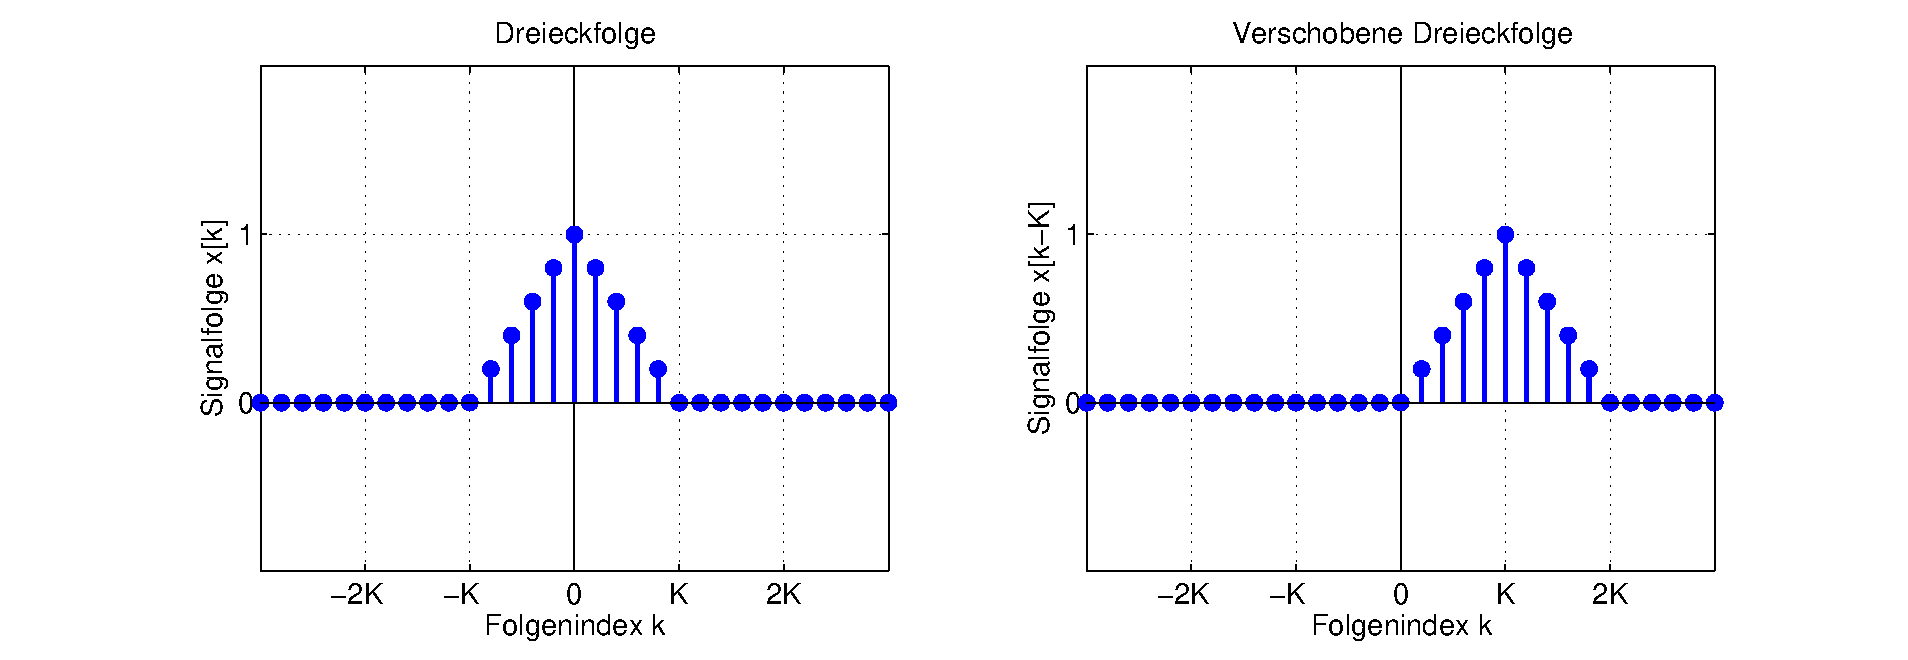
\includegraphics[width=0.5\textwidth]{Kapitel3/Bilder/image13}}
  \caption{Box-Plot f\"{u}r die Stichproben aus \ref{fig:DefinitionSchiefe}}
  \label{fig:DefinitionSchiefeBoxPlot}
\end{figure}

\noindent MATLAB und python Python bieten zur Erstellung eines Box-Plots eine separate Funktion an.

\begin{table}[H]
\setlength{\arrayrulewidth}{.1em}
\caption{Darstellung des Box-Plots einer Stichprobe in MATLAB}
\setlength{\fboxsep}{0pt}%
\colorbox{lightgray}{%
\arrayrulecolor{white}%
\begin{tabular}{| c | c |}
\hline
\parbox[c][0.3in][c]{3.3in}{\smallskip\centering\textbf{\fontfamily{phv}\selectfont{Darstellung}}} & 
\parbox[c][0.3in][c]{3.3in}{\smallskip\centering\textbf{\fontfamily{phv}\selectfont{MATLAB-Befehl}}}\\ \hline

\parbox[c][0.3in][c]{3.3in}{\centering\fontfamily{phv}\selectfont{Box-Plot}} & 
\parbox[c][0.3in][c]{3.3in}{\centering\fontfamily{phv}\selectfont{boxplot(x)}}\\ \hline

\end{tabular}%
}
\label{tab:threetwentyone}
\end{table}

\begin{table}[H]
\setlength{\arrayrulewidth}{.1em}
\caption{Darstellung des Box-Plots einer Stichprobe in Python}
\setlength{\fboxsep}{0pt}%
\colorbox{lightgray}{%
\arrayrulecolor{white}%
\begin{tabular}{| c | c |}
\hline
\parbox[c][0.3in][c]{3.3in}{\smallskip\centering\textbf{\fontfamily{phv}\selectfont{Darstellung}}} & 
\parbox[c][0.3in][c]{3.3in}{\smallskip\centering\textbf{\fontfamily{phv}\selectfont{MATLAB-Befehl}}}\\ \hline

\parbox[c][0.3in][c]{3.3in}{\centering\fontfamily{phv}\selectfont{Box-Plot}} & 
\parbox[c][0.3in][c]{3.3in}{\centering\fontfamily{phv}\selectfont{matplotlib.pyplot.boxplot}}\\ \hline

\end{tabular}%
}
\label{tab:threetwentytwo}
\end{table}

\clearpage

\subsection{Anwendungsbeispiel: Charakterisierung eines Klebeprozesses}

\noindent Eine Automatisierungseinrichtung hat zum Befestigen einer Folie im Automobilbau Klebermengen dosiert. Die in Tabelle 3.23Tabelle 3.23 enthaltenen Zahlenwerte stellen eine Stichprobe mit einem Umfang von N = 40 abgef\"{u}llten Klebermengen dar. 

\begin{table}[H]
\setlength{\arrayrulewidth}{.1em}
\caption{Stichprobenwerte zur Bewertung eines Klebeprozesses}
\setlength{\fboxsep}{0pt}%
\colorbox{lightgray}{%
\arrayrulecolor{white}%
\begin{tabular}{| wc{4cm} | wc{2cm} | wc{2cm} | wc{2cm} | wc{2cm} | wc{2cm} }
\hline\xrowht{15pt}

\fontfamily{phv}\selectfont\textbf{Messung} & \multicolumn{5}{c}{\fontfamily{phv}\selectfont\textbf{Messwerte Klebermenge m / mg}} \\ \hline \xrowht{15pt}

\fontfamily{phv}\selectfont\textbf{1 - 5} &
50.18 & 51.85 & 51.09 & 50.09 & 51.03\\ \hline\xrowht{15pt}

\fontfamily{phv}\selectfont\textbf{6 - 10} & 
50.69 & 51.76 & 51.23 & 51.49 & 51.62\\ \hline\xrowht{15pt}

\fontfamily{phv}\selectfont\textbf{11- 15} &
50.52 & 51.33 & 51.18 & 51.76 & 52.62\\ \hline\xrowht{15pt}

\fontfamily{phv}\selectfont\textbf{16 - 20} &
51.49 & 51.19 & 51.28 & 50.82 & 50.01\\ \hline\xrowht{15pt}

\fontfamily{phv}\selectfont\textbf{21 - 25} &
51.6 & 50.94 & 51.54 & 51.3 & 50.91\\ \hline\xrowht{15pt}

\fontfamily{phv}\selectfont\textbf{26 - 30} &
51.44 & 51.78 & 51.37 & 51.36 & 50.54\\ \hline\xrowht{15pt}

\fontfamily{phv}\selectfont\textbf{31 - 35} &
52.2 & 52.12 & 49.4 & 49.76 & 51.54\\ \hline\xrowht{15pt}

\fontfamily{phv}\selectfont\textbf{36 - 40} &
50.64 & 50.37 & 50.16 & 50.61 & 50.38\\ \hline 

\end{tabular}%
}
\label{tab:threetwentythree}
\end{table}

\noindent Der Datensatz wird im Folgenden ohne Aufteilung der Daten in Klassen und mit Aufteilung der Daten in Klassen ausgewertet. Abschlie{\ss}end werden die Ergebnisse miteinander verglichen.


\subsubsection{Datenanalyse in MATLAB ohne Aufteilung der Daten in Klassen}

\noindent Bei dem untersuchten Klebeprozess handelt es sich um einen kontinuierlichen Prozess, jeder Messwert besitzt hierbei die absolute H\"{a}ufigkeit 1. Eine Darstellung als H\"{a}ufigkeitsverteilung l\"{a}sst somit keine R\"{u}ckschl\"{u}sse auf den zu untersuchenden Prozess zu. Deshalb werden die Daten mit einem Streudiagramm und der relativen Summenh\"{a}ufigkeit beschrieben.

\begin{figure}[H]
  \centerline{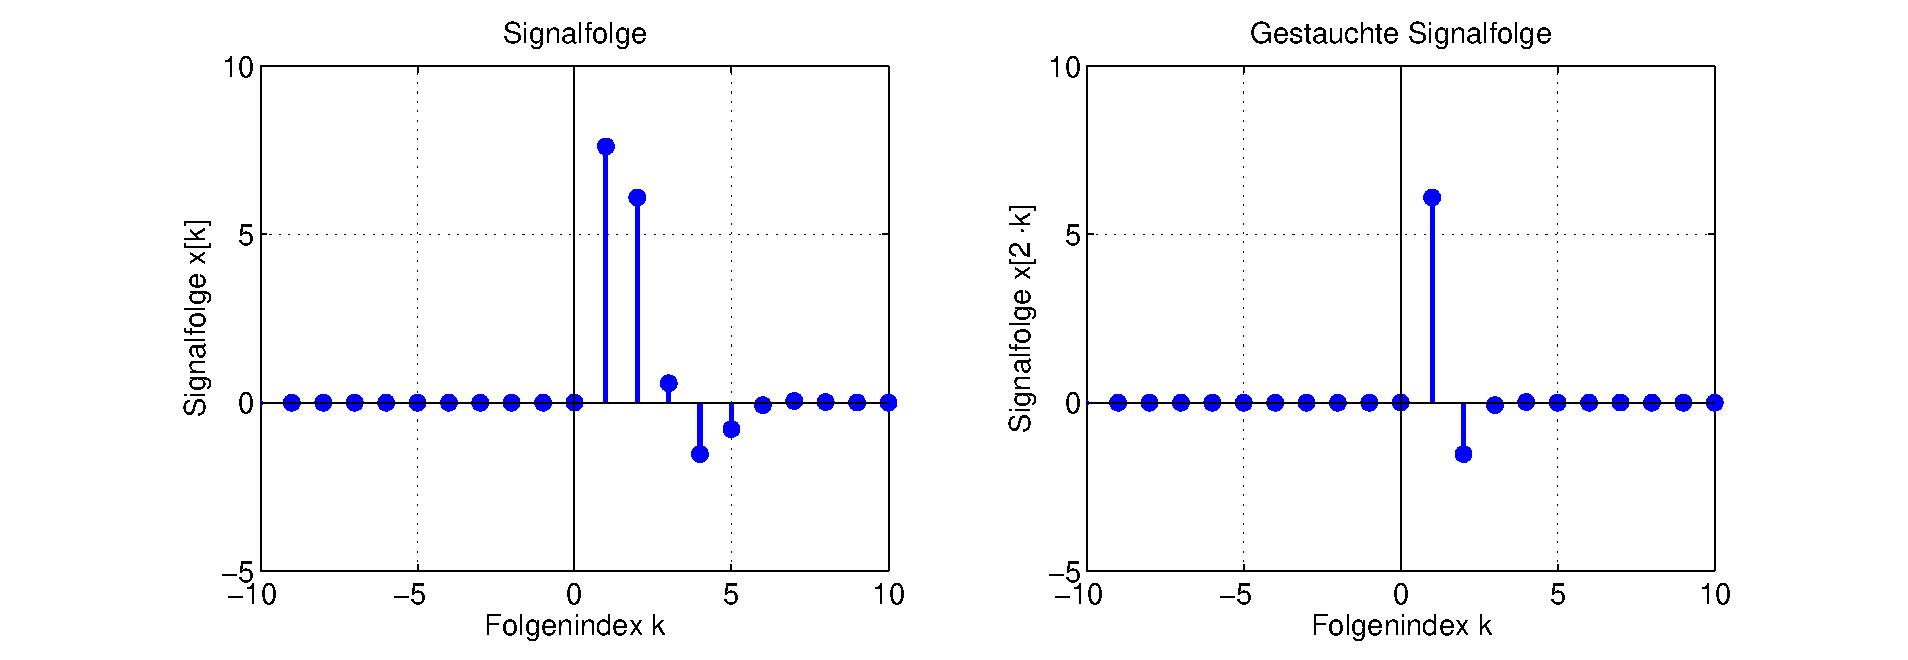
\includegraphics[width=1\textwidth]{Kapitel3/Bilder/image14}}
  \caption{Darstellung der Messwerte als Streudiagramm und als relative Summenh\"{a}ufigkeit}
  \label{fig:Streudiagramm}
\end{figure}

\noindent Im Streudiagramm in Bild \ref{fig:Streudiagramm} ist zu erkennen, dass sich die Messwerte in einem Bereich von 49 bis 53 mg befinden. In der Darstellung der relativen Summenh\"{a}ufigkeit kann abgelesen werden, dass der Median mit einer relativen Summenh\"{a}ufigkeit von 0.5 bei einer Klebemenge von 51.25 mg liegt. Die Grafik wurde mit dem folgenden MATLAB-Code erzeugt.

\clearpage

\lstinputlisting[caption = {}]{Kapitel3/mat1.m}

\noindent Um die Lage der Messwerte genauer zu beschreiben, werden die in Abschnitt 3.3.1 eingef\"{u}hrten Lagekennwerte berechnet. F\"{u}r die Messwerte aus Tabelle \ref{tab:threetwentythree} ergibt sich der arithmetische Mittelwert zu

\begin{equation}\label{eq:threesixtyeight}
\bar{m}=\dfrac{1}{N} \cdot \sum _{n=1}^{N}m_{n}  =51.08 mg
\end{equation}

\noindent Der Median wird nach Sortieren der Messwerte aus dem Mittelwert der beiden mittleren Messwerte bestimmt.

\begin{equation}\label{eq:threesixtynine}
m_{MED} =\dfrac{m_{17} +m_{8} }{2} =\dfrac{51.19 mg + 51.23 mg}{2} =51.21mg
\end{equation}

\noindent Zus\"{a}tzlich zu den Kennwerten zur Beschreibung der Lage werden in Abschnitt 3.3.2 Streuungskennwerte definiert. Die Varianz der Messwerte berechnet sich zu

\begin{equation}\label{eq:threeseventy}
s^{2} =\dfrac{1}{N-1} \cdot \sum _{n=1}^{N}\left(m_{n} -\bar{m}\right)^{2}  =  0.49 mg^{2}
\end{equation}

\noindent Aus der Wurzel der Varianz folgt die Standardabweichung von

\begin{equation}\label{eq:threeseventyone}
s=\sqrt{s^{2}} = 0.70 mg
\end{equation}

\noindent Der Interquartilabstand ergibt sich aus der Differenz des 75\%-Quartils und des 25\%-Quartils der Messwerte zu

\begin{equation}\label{eq:threeseventytwo}
IQR=m_{0.75} -m_{0.25} =50.57 mg-51.54 mg= 0.97 mg
\end{equation}

\clearpage 

\noindent Der verwendete Programmcode zur Berechnung der Lage- und Streuungskennwerte mithilfe von MATLAB ist im Folgenden dargestellt.

\lstinputlisting[caption = {}]{Kapitel3/mat2.m}

\noindent Da aus Bild \ref{fig:DefinitionSchiefeBoxPlot2} keine Aussage hinsichtlich der Schiefe der Verteilung gemacht werden kann, wird der 25\%-Quartilkoeffizient und der Momentenkoeffizient der Schiefe zur Bewertung herangezogen. Der 25\%-Quartilkoeffizient der Schiefe berechnet sich zu

\begin{equation}\label{eq:threeseventythree}
g_{0.25} =\dfrac{\left(m_{0.75} -m_{MED} \right)-\left(m_{MED} -m_{0.25} \right)}{m_{0.75} -m_{0.25}} =\dfrac{\left(51.54-51.21\right)-\left(51.21-50.57\right)}{51.54-50.57} =-0.32
\end{equation}

\noindent und der Momentenkoeffizient der Schiefe folgt zu

\begin{equation}\label{eq:threeseventyfour}
g_{M} =\dfrac{\dfrac{1}{N} \cdot \displaystyle\sum\limits _{n=1}^{N}\left(m_{n} -\bar{m}\right)^{3}}{s^{3}} =-0.28
\end{equation}

\noindent Beide Werte weisen auf eine linksschiefe Verteilung hin. Die Berechnung der Kennwerte der Schiefe wird mit MATLAB mit der folgenden Befehlssequenz durchgef\"{u}hrt

\lstinputlisting[caption = {}]{Kapitel3/mat3.m}

\noindent Der Klebeprozess wird mit den Stichprobenwerten aus Tabelle \ref{tab:threetwentythree} sowohl grafisch dargestellt als auch durch Kennwerte beschrieben. Dabei werden die Daten nicht in Klassen eingeteilt. Um den Unterschied zu zeigen, wird auf Basis der gleichen Stichprobenwerte nun eine Datenanalyse durchgef\"{u}hrt, bei der die Messwerte in Klassen eingeteilt werden.


\subsubsection{Datenanalyse in MATLAB mit Aufteilung der Daten in Klassen}

\noindent Zun\"{a}chst muss f\"{u}r die Daten eine sinnvolle Klasseneinteilung gefunden werden. Hierbei wird insbesondere darauf geachtet, dass die Klassenmitten m\"{o}glichst Zahlen mit wenig Nachkommastellen sind. Bei dem Datensatz aus Tabelle \ref{tab:threetwentythree} mit einem Minimalwert von m$_{MIN}$ = 49.40 mg und einem Maximalwert von m$_{MAX}$ = 52.62 mg bietet es sich an, eine Klassenbreite d von 1 mg zu w\"{a}hlen. Die Messwerte lassen sich damit in 5 Klassen einteilen, die in Tabelle \ref{tab:threetwentyfour} zusammen mit ihrer absoluten und ihrer relativen H\"{a}ufigkeit angegeben sind.

\clearpage

\begin{table}[H]
\setlength{\arrayrulewidth}{.1em}
\caption{Stichprobenwerte zur \"{U}berpr\"{u}fung eines Klebeprozesses eingeteilt in Klassen}
\setlength{\fboxsep}{0pt}%
\colorbox{lightgray}{%
\arrayrulecolor{white}%
\begin{tabular}{| c | c | c | c | c |}
\hline
\parbox[c][0.6in][c]{1.2in}{\smallskip\centering\textbf{\fontfamily{phv}\selectfont{c / mg}}} & 
\parbox[c][0.6in][c]{1.2in}{\smallskip\centering\textbf{\fontfamily{phv}\selectfont{Anzahl Häufigkeit h$_{\mathbf{A}}$(c)}}} & 
\parbox[c][0.6in][c]{1.2in}{\smallskip\centering\textbf{\fontfamily{phv}\selectfont{Relative Häufigkeit h(c)}}} & 
\parbox[c][0.6in][c]{1.2in}{\smallskip\centering\textbf{\fontfamily{phv}\selectfont{Absolute Summenhäufigkeit H$_{\mathbf{A}}$(c)}}} & 
\parbox[c][0.6in][c]{1.2in}{\smallskip\centering\textbf{\fontfamily{phv}\selectfont{Relative Summenhäufigkeit H(c)}}}\\ \hline

\parbox[c][0.3in][c]{1.2in}{\centering\textbf{49}} & 
\parbox[c][0.3in][c]{1.2in}{\centering{1}} & 
\parbox[c][0.3in][c]{1.2in}{\centering{0.025}} & 
\parbox[c][0.3in][c]{1.2in}{\centering{1}} & 
\parbox[c][0.3in][c]{1.2in}{\centering{0.025}}\\ \hline

\parbox[c][0.3in][c]{1.2in}{\centering\textbf{50}} & 
\parbox[c][0.3in][c]{1.2in}{\centering{7}} & 
\parbox[c][0.3in][c]{1.2in}{\centering{0.175}} & 
\parbox[c][0.3in][c]{1.2in}{\centering{8}} & 
\parbox[c][0.3in][c]{1.2in}{\centering{0.2}}\\ \hline

\parbox[c][0.3in][c]{1.2in}{\centering\textbf{51}} & 
\parbox[c][0.3in][c]{1.2in}{\centering{21}} & 
\parbox[c][0.3in][c]{1.2in}{\centering{0.525}} & 
\parbox[c][0.3in][c]{1.2in}{\centering{29}} & 
\parbox[c][0.3in][c]{1.2in}{\centering{0.725}}\\ \hline

\parbox[c][0.3in][c]{1.2in}{\centering\textbf{52}} & 
\parbox[c][0.3in][c]{1.2in}{\centering{10}} & 
\parbox[c][0.3in][c]{1.2in}{\centering{0.25}} & 
\parbox[c][0.3in][c]{1.2in}{\centering{39}} & 
\parbox[c][0.3in][c]{1.2in}{\centering{0.975}}\\ \hline

\parbox[c][0.3in][c]{1.2in}{\centering\textbf{53}} & 
\parbox[c][0.3in][c]{1.2in}{\centering{1}} & 
\parbox[c][0.3in][c]{1.2in}{\centering{0.025}} & 
\parbox[c][0.3in][c]{1.2in}{\centering{40}} & 
\parbox[c][0.3in][c]{1.2in}{\centering{1}}\\ \hline

\end{tabular}%
}
\label{tab:threetwentyfour}
\end{table}

\noindent Die relative H\"{a}ufigkeit und die relative Summenh\"{a}ufigkeit der in Klassen eingeteilten Stichprobenwerte sind in Bild \ref{fig:DefinitionSchiefeBoxPlot2} dargestellt.

\noindent 
\begin{figure}[H]
  \centerline{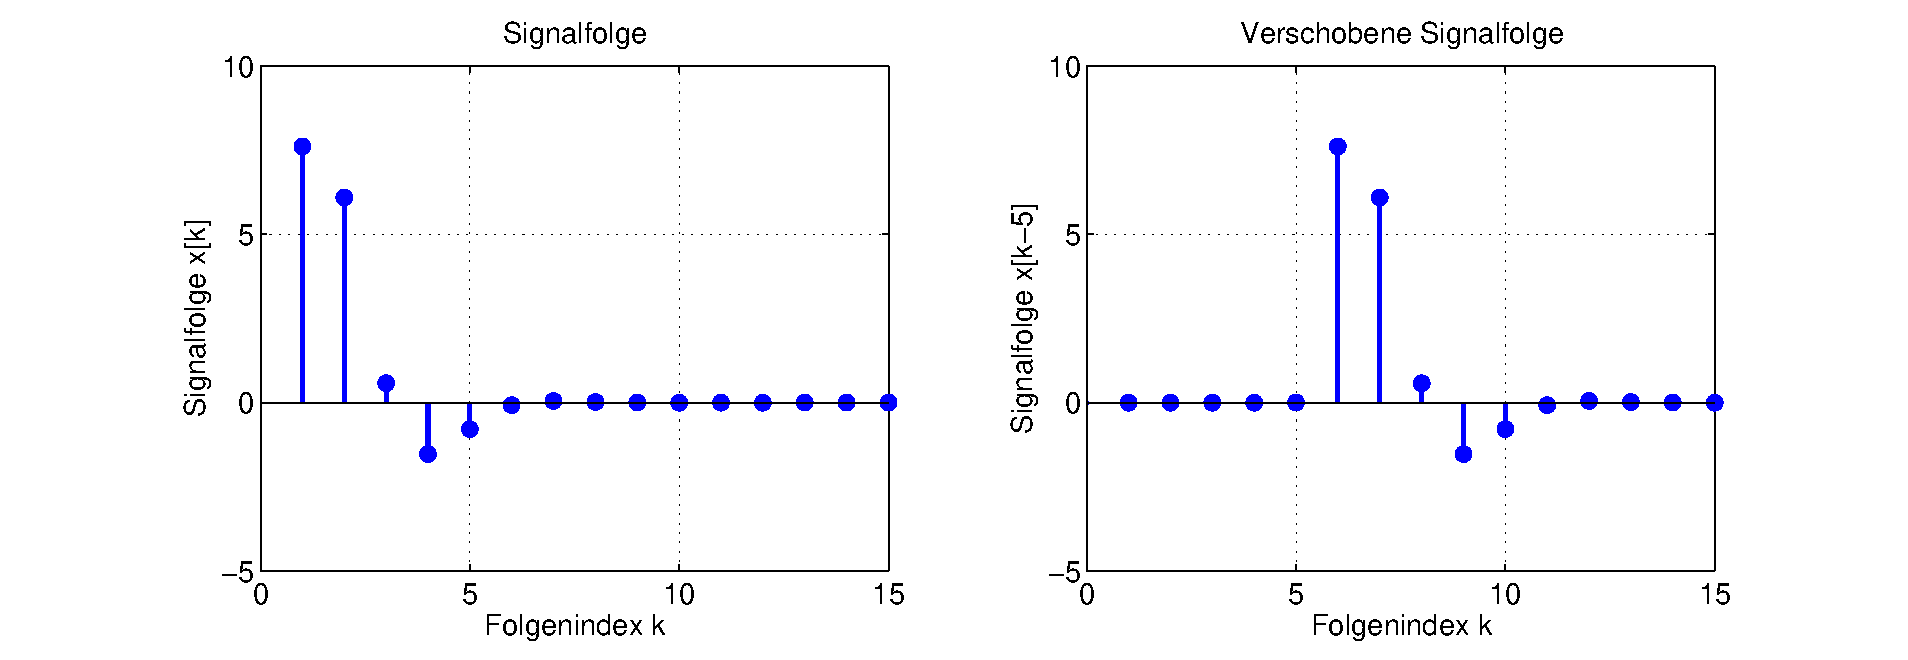
\includegraphics[width=1\textwidth]{Kapitel3/Bilder/image15}}
  \caption{Darstellung der relativen H\"{a}ufigkeit und der relativen Summenh\"{a}ufigkeit}
  \label{fig:DefinitionSchiefeBoxPlot2}
\end{figure}

\noindent Die Einteilung der Messwerte in Klassen erfolgt durch MATLAB. Die Berechnung der H\"{a}ufigkeiten und die Darstellung in Bild \ref{fig:DefinitionSchiefeBoxPlot2} werden mit der folgenden MATLAB-Befehlssequenz erstellt.

\lstinputlisting[caption = {}]{Kapitel3/mat4.m}

\noindent Zur numerischen Beschreibung der H\"{a}ufigkeitsverteilung werden analog zur Datenanalyse ohne Klasseneinteilung die Lage- und Streuungskennwerte berechnet. Hierbei muss die Klasseneinteilung der Messwerte ber\"{u}cksichtigt werden. Damit berechnet sich der arithmetische Mittelwert zu

\begin{equation}\label{eq:threeseventyfive}
\bar{m}=\displaystyle\sum _{n=1}^{N}\left(c_{n} \cdot h (c_{n})\right) =51.08 mg
\end{equation}

\noindent Der Median folgt nach den Darstellungen in Abschnitt 3.3.1 zu

\begin{equation}\label{eq:threeseventysix}
m_{MED} =c_{n-1} +\dfrac{d\cdot \left(0.5-H(c_{n-1} )\right)}{h\left(c_{n} \right)} =50 mg+\dfrac{1 mg\cdot (0.5-0.2)}{0.525} = 50.57 mg
\end{equation}

\noindent Die Berechnung der Streuungskennwerte f\"{u}hren zu einem Wert f\"{u}r die Varianz von

\begin{equation}\label{eq:threeseventyseven}
s^{2} =\dfrac{1}{N-1} \cdot \displaystyle\sum _{n=1}^{N}\left(h_{a} (c_{n})\cdot (c_{n} -\bar{m})^{2} \right) =6.19 mg^{2}
\end{equation}

\noindent und f\"{u}r die Standardabweichung von

\begin{equation}\label{eq:threeseventyeight}
s=\sqrt{s^{2} } =2.49 mg
\end{equation}

\noindent Der Interquartilabstand berechnet sich aus der Differenz aus dem 75\%-Quartil

\begin{equation}\label{eq:threeseventynine}
m_{0.75} =c_{n-1} +\dfrac{d\cdot \left(0.75-H\left(c_{n-1} \right)\right)}{h(c_{n})} =51 mg+\dfrac{1 mg\cdot (0.75-0.725)}{0.25} =51.10 mg
\end{equation}

\noindent und dem 25\%-Quartil

\begin{equation}\label{eq:threeeighty}
m_{0.25} =c_{n-1} +\dfrac{d\cdot \left(0.25-H(c_{n-1} )\right)}{h(c_{n})} =50 mg+\dfrac{1 mg\cdot \left(0.25-0.2\right)}{0.525} =50.0952 mg
\end{equation}

\noindent zu

\begin{equation}\label{eq:threeeightyone}
IQR=m_{0.75} -m_{0.25} =51.10 mg-50.0952 mg=1.00 mg
\end{equation}

\noindent Zur numerischen Auswertung der Daten wird die folgende Befehlssequenz verwendet.

\lstinputlisting[caption = {}]{Kapitel3/mat5.m}

\noindent Abschlie{\ss}end wird die Schiefe der H\"{a}ufigkeitsverteilung beurteilt. Bereits in Bild \ref{fig:DefinitionSchiefeBoxPlot2} ist ersichtlich, dass die Verteilung der relativen H\"{a}ufigkeit nahezu symmetrisch zu der Klasse von 51 mg ist. Es ist daher zu erwarten, dass sowohl der 25\%-Quartilkoeffizient als auch der Momentenkoeffizient der Schiefe einen Wert nahe 0 annehmen. Die Berechnung zeigt, dass sowohl der 25\%-Quartilkoeffizient der Schiefe mit

\begin{equation}\label{eq:threeeightytwo}
g_{0.25} =\dfrac{(m_{0.75} -m_{med})-(m_{med} -m_{0.25} )}{m_{0.75} -m_{0.25}}=\dfrac{(51.10-50.57)-(50.57-50.0952)}{51.10-50.0952} = 0.05
\end{equation}

\noindent als auch der Momentenkoeffizient der Schiefe mit

\begin{equation}\label{eq:threeeightythree}
g_{M} =\dfrac{\dfrac{1}{N} \cdot \sum _{n=1}^{N}(h_{a} (c_{n} )\cdot (c_{n} -\bar{m})^{3}) }{s^{3} } =-0.03
\end{equation}

\noindent diese Aussage bekr\"{a}ftigt. Die Berechnung mit MATLAB ergibt sich aus folgender Befehlssequenz.

\lstinputlisting[caption = {}]{Kapitel3/mat6.m}

\subsubsection{Vergleich der beiden Datenanalysen}

\noindent Die Daten aus Tabelle \ref{tab:threetwentythree} werden ohne eine Einteilung in Klassen und mit einer Einteilung in f\"{u}nf Klassen bewertet. Hierzu werden die eingef\"{u}hrten Lage- und Streuungskennwerte berechnet und die Gr\"{o}{\ss}en zur Bewertung der Schiefe bestimmt. Dabei weichen die Ergebnisse zwischen den beiden Analysemethoden voneinander ab. Um den Unterschied grafisch zu verdeutlichen, werden die Kennwerte der Datenanalyse mit und ohne eine Einteilung in Klassen als Box-Plot in \ref{fig:DefinitionSchiefeBoxPlot3} zusammengefasst und gegen\"{u}bergestellt.

\noindent 
\begin{figure}[H]
  \centerline{\includegraphics[width=1\textwidth]{Kapitel3/Bilder/image16}}
  \caption{Gegen\"{u}berstellung der beiden Datenanalysemethoden}
  \label{fig:DefinitionSchiefeBoxPlot3}
\end{figure}

\noindent Anhand des blauen Rechtecks in der Grafik des Box-Plots kann abgelesen werden, in welchem Bereich 50 \% der Stichprobenwerte liegen, die rote Linie kennzeichnet den Median der Verteilung. In \ref{fig:DefinitionSchiefeBoxPlot3} ist gut zu erkennen, dass die Auswertungen mit und ohne Klassenbildung stark voneinander abweichen. W\"{a}hrend der Median f\"{u}r den Klebeprozess ohne Klassenbildung bei m$_{MED}$ = 51.21 mg liegt, liegt er nach der Einteilung in Klassen bei m$_{MED}$ = 50.57 mg, der Wert differiert um 0.7 mg. Au{\ss}erdem ist zu erkennen, dass die Spannweite der Verteilung bei einer Betrachtung mit einer Einteilung in Klassen bei der vorliegenden Wahl der Klassenmitten gr\"{o}{\ss}er ist als bei einer Betrachtung ohne eine Einteilung in Klassen.\newline

\noindent Die unterschiedlichen Ergebnisse erkl\"{a}ren sich dadurch, dass mit der Klassenbildung die einzelnen Werte nicht mehr erfasst werden und dadurch Informationen \"{u}ber die Verteilung verloren gehen. Die Genauigkeit der Auswertung ist von der Klassenanzahl abh\"{a}ngig. Je weniger Klassen aus der Urliste gebildet werden, desto mehr Informationen gehen verloren und desto st\"{a}rker k\"{o}nnen die berechneten Kenngr\"{o}{\ss}en von den wahren Kenngr\"{o}{\ss}en der zu Grunde liegenden Verteilung abweichen. Aus diesem Grund sollte nach M\"{o}glichkeit stets mit der Urliste gearbeitet werden. \newline

\noindent Der verwendete Programmcode zur Darstellung des Box-Plots f\"{u}r die Messdaten ohne eine Einteilung in Klassen kann in MATLAB der folgenden Auflistung entnommen werden.

\lstinputlisting[caption = {}]{Kapitel3/mat7.m}

\noindent Der Box-Plot f\"{u}r die Zusammenfassung der Datenanalyse mit Einteilung in Klassen muss unter Verwendung der berechneten Kenngr\"{o}{\ss}en manuell programmiert werden, da MATLAB keine Funktionen zur Berechnung von Kenngr\"{o}{\ss}en gruppierter Daten zur Verf\"{u}gung stellt.

\subsubsection{Programmbeispiel zur Datenanalyse in Python}

\noindent Die Datenanalyse in Python erfordert zun\"{a}chste das Laden der erforderlichen Module und eine Definition des Ortes, an dem die Grafiken angezeigt werden sollen.

\lstinputlisting[caption = {}]{Kapitel3/mat8.m}

\noindent Die Daten liegen als mat-Datei vor. Python bietet einen Befehl zum Laden dieser Daten an. Die Daten werden in ein eindimensionales Array gewandelt.

\lstinputlisting[caption = {}]{Kapitel3/mat9.m}

\noindent Der Datenumfang und die statistischen Kennwerte werden mit den angegebenen Befehlen berechnet. Dabei werden die in MATLAB berechneten Ergebnisse best\"{a}tigt.

\lstinputlisting[caption = {}]{Kapitel3/mat10.m}

\noindent Die Daten werden mit einem Streudiagramm sowie einem Boxplot visualisiert.

\noindent 
\begin{figure}[H]
  \centerline{\includegraphics[width=1\textwidth]{Kapitel3/Bilder/image17}}
  \caption{Darstellung der Messwerte als Streudiagramm und Boxplot}
  \label{fig:Inconnue}
\end{figure}

\lstinputlisting[caption = {}]{Kapitel3/mat11.m}

\noindent Der steige Datensatz wird mit Hilfe von dem Modul Pandas in eine Tabelle gewandelt und ausgegeben. Dabei werden absolute und relative H\"{a}ufigkeit sowie die absolute und relative H\"{a}ufigkeit berechnet.

\clearpage

\lstinputlisting[caption = {}]{Kapitel3/mat12.m}

\noindent Das Ergebnis wird als Histogramm und mit seienr relativen Summenh\"{a}ufigkeit dargestellt.

\noindent 
\begin{figure}[H]
  \centerline{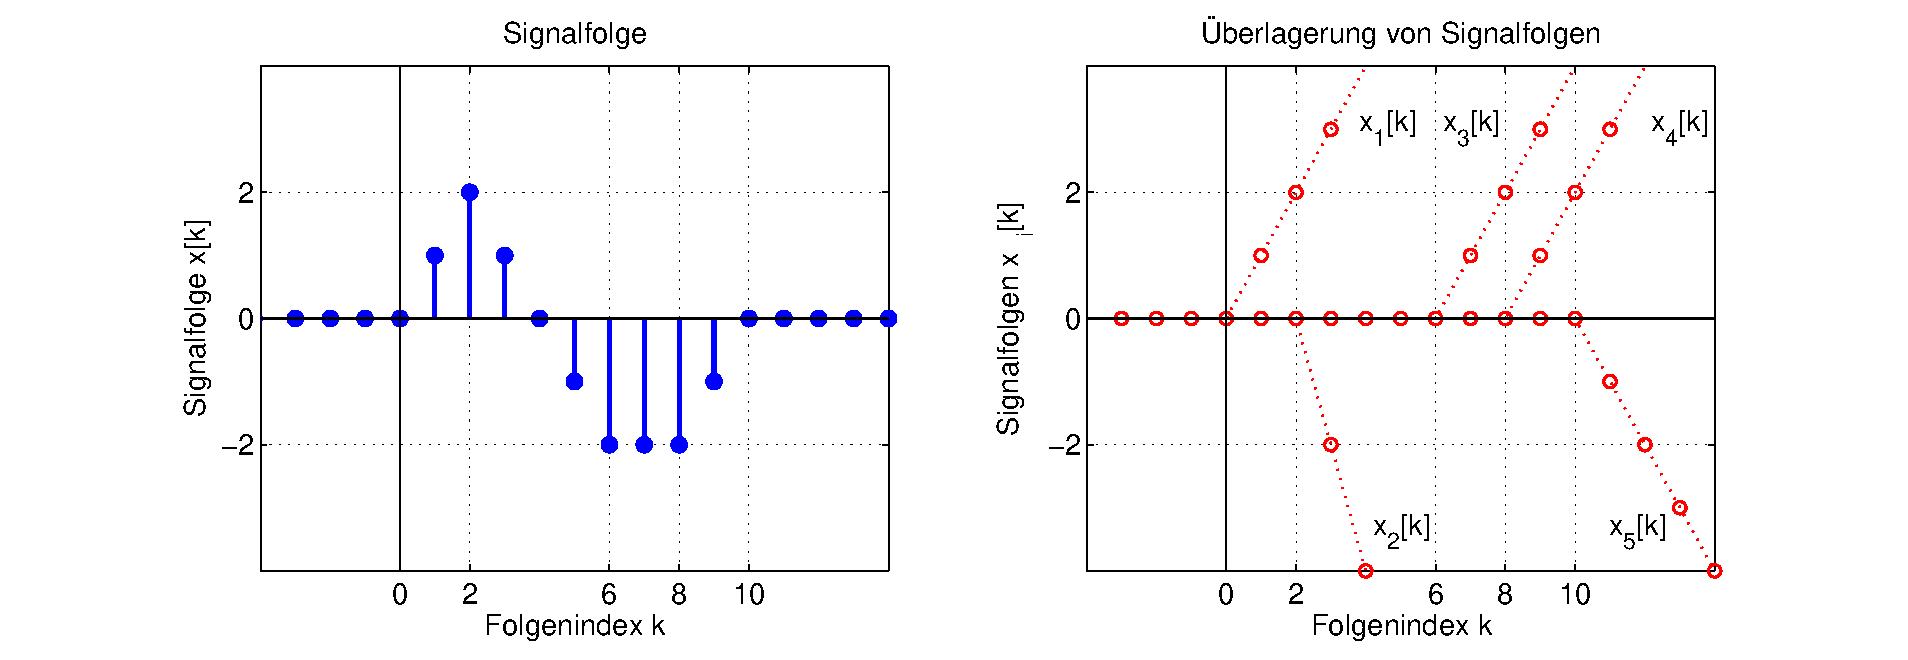
\includegraphics[width=1\textwidth]{Kapitel3/Bilder/image18}}
  \caption{Darstellung der Messwerte als Histogramm und relative Summenh\"{a}ufigkeit}
  \label{fig:AnwendungsbeispielKlebermenge1}
\end{figure}

\lstinputlisting[caption = {}]{Kapitel3/mat13.m}

\clearpage


\subsection{Literatur}

\begin{tabular}{|p{0.6in}|p{5.7in}|} \hline 
[Krey91] & Kreyszig, Erwin: Statistische Methoden und ihre Anwendungen\newline 
4., unver\"{a}nderter Nachdruck der 7. Auflage\newline 
Vandenhoeck \& Ruprecht, G\"{o}ttingen, 1991\\ \hline 
[Fahr06] & Fahrmeir, Ludwig; K\"{u}nstler, Rita; Pigeot, Iris; Tutz, Gerhard: Der Weg zur Datenanalyse\newline 
6. Auflage\newline 
Springer Berlin Heidelberg New York, 2006 \\ \hline 
[Ross06] & Ross, M. Sheldon: Statistik f\"{u}r Ingenieure und Naturwissenschaftler\newline 
3. Auflage\newline 
Spektrum Akademischer Verlag, M\"{u}nchen, 2006 \\ \hline 
\end{tabular}


\clearpage

\section{Zeitdiskrete Systeme im Zeitbereich}\label{four}
\noindent Wahrscheinlichkeitsverteilungen geben an, mit welcher Wahrscheinlichkeit unterschiedliche Zufallsereignisse eintreffen. Sie beschreiben diese Eintreffwahrscheinlichkeit als Funktion einer sogenannten Zufallsvariable. Die Wahrscheinlichkeitsverteilung stellt damit das theoretische Gegenst\"{u}ck zur empirischen H\"{a}ufigkeitsverteilung dar, die sich aus der Analyse vorhandener Daten wie zum Beispiel Messwerten ergibt.\newline

\noindent Wie bei H\"{a}ufigkeitsverteilungen wird zwischen diskreten und stetigen Wahrscheinlichkeitsverteilungen unterschieden. Beispiel f\"{u}r eine diskrete Verteilung ist die Hypergeometrische Verteilung, die in der Qualit\"{a}tssicherung bei Stichproben-Eingangspr\"{u}fungen eingesetzt wird. Viele Prozesse und Produktmerkmale werden aber \"{u}ber stetige Zufallsvariablen beschrieben. Deshalb basieren viele Methoden des Design For Six Sigma auf stetigen Zufallsvariablen und damit auf stetigen Verteilungen. Der wichtigste Vertreter von stetigen Verteilungen ist die Normalverteilung, mit der sich viele reale Zufallsprozesse approximativ beschreiben lassen.\newline

\noindent Nach der Einf\"{u}hrung des Begriffes der Zufallsvariablen und ihrer Verteilungen werden Kenngr\"{o}{\ss}en von Wahrscheinlichkeitsverteilungen berechnet. Diese Erkenntnisse werden anschlie{\ss}end an speziellen diskreten und stetigen Verteilungen angewendet.\newline

\subsection{Zufallsvariablen und Wahrscheinlichkeitsverteilungen}

\subsubsection{Zufallsvariablen}

\noindent Als Zufallsvariable wird allgemein eine Variable bezeichnet, die das Ergebnis eines Zufallsexperimentes repr\"{a}sentiert. Zum Beispiel kann bei einem W\"{u}rfelexperiment mit zwei W\"{u}rfeln das Zufallsergebnis \"{u}ber die Summe der beiden Augenzahlen dargestellt werden. Bei einem Prozess mit stetigen Ergebniswerten, wie zum Beispiel der Fertigung von Widerst\"{a}nden, wird die Abweichung vom Sollwert durch eine Zufallsvariable beschrieben. Aber auch, wenn die bei einem Experiment denkbaren Ereignisse nicht direkt mit Zahlen beschrieben werden, kann jedem m\"{o}glichen Ereignis eine Zahl zugeordnet werden. Diese Zahl gibt im einfachsten Fall den Index der Menge an, zu dem das Ergebnis des Zufallsexperimentes geh\"{o}rt. Zum Beispiel k\"{o}nnen die Permutationen der Buchstaben a, b und c in Gruppen eingeteilt werden, die einer Zufallsvariable x zugeordnet werden.

\begin{table}[H]
\setlength{\arrayrulewidth}{.1em}
\caption{Zuordnung von Zufallsereignissen zu einer Zufallsvariablen x}
\setlength{\fboxsep}{0pt}%
\colorbox{lightgray}{%
\arrayrulecolor{white}%
\begin{tabular}{| l | l |}
\hline
\parbox[c][0.28in][c]{3.3in}{\smallskip\centering\textbf{\fontfamily{phv}\selectfont{Zufallsvariable x}}} & 
\parbox[c][0.28in][c]{3.3in}{\smallskip\centering\textbf{\fontfamily{phv}\selectfont{Ergebnis des Experimentes}}}\\ \hline

\parbox[c][0.5in][c]{3.3in}{\centering\fontfamily{phv}\selectfont{1}} 
& 
\parbox[c][0.5in][c]{3.3in}{\centering\fontfamily{phv}\selectfont{abc\\ bac}}\\ \hline

\parbox[c][0.5in][c]{3.3in}{\centering\fontfamily{phv}\selectfont{2}} & 
\parbox[c][0.5in][c]{3.3in}{\centering\fontfamily{phv}\selectfont{cab\\ acb}}\\ \hline

\parbox[c][0.5in][c]{3.3in}{\centering\fontfamily{phv}\selectfont{3}} & 
\parbox[c][0.5in][c]{3.3in}{\centering\fontfamily{phv}\selectfont{bca\\ cba}}\\ \hline

\end{tabular}%
}
\label{tab:fourone}
\end{table}

\noindent In jedem dieser Beispiele kann die Zufallsvariable x verschiedene Werte annehmen. Aber es l\"{a}sst sich nicht vorhersagen, welchen Wert die Zufallsvariable annehmen wird, da dieser Wert vom Einfluss unkontrollierbarer Umst\"{a}nde abh\"{a}ngt.\newline

\noindent Zufallsvariablen k\"{o}nnen in die gleichen Gruppen eingeteilt werden, wie die Merkmalstypen bei der beschreibenden Statistik. Stetige Merkmalstypen entsprechen stetigen Zufallsvariablen, diskrete Merkmalstypen sowie ordinale und gruppierende Merkmalstypen werden \"{u}ber diskrete Zufallsvariablen abgebildet. \newline

\noindent Mathematisch wird einem Zufallsexperiment eine Zufallsvariable x zugeordnet, die folgende Eigenschaften besitzen muss:

\begin{itemize}
    \item   Die Werte von x sind reelle Zahlen.
    \item  F\"{u}r jede Zahl a und f\"{u}r jedes Intervall I ist die Wahrscheinlichkeit des Ereignisses x = a und x $\in$ I im Einklang mit den Axiomen der Wahrscheinlichkeit.
\end{itemize}

\noindent
\colorbox{lightgray}{%
\arrayrulecolor{white}%
\renewcommand\arraystretch{0.6}%
\begin{tabular}{ wl{16.5cm} }
{\fontfamily{phv}\selectfont{Beispiel: W\"{u}rfelexperiment}}
\end{tabular}%
}\medskip

\noindent Anhand des Zufallsexperimentes W\"{u}rfeln mit zwei W\"{u}rfeln wird der zweite Teil der Definition erl\"{a}utert. Die Zufallsvariable x stellt die Summe der beiden Augenzahlen dar. Die Wahrscheinlichkeit P(x = 2) ist die Wahrscheinlichkeit, dass das Ergebnis des Zufallsexperiments die Augenzahl 2 ist. Da dieses Ergebnis nur erreicht wird, wenn zweimal die Augenzahl 1 erscheint, ist die Wahrscheinlichkeit

\begin{equation}\label{eq:fourone}
P(x=2)=\dfrac{1}{6} \cdot \dfrac{1}{6} =\dfrac{1}{36} <1   
\end{equation}

\noindent Auch f\"{u}r jedes andere Zufallsereignis des Experimentes liegt die Wahrscheinlichkeit im Bereich 0 $\leq$ P $\leq$ 1. Das sichere Ereignis ist, dass die Summe der Augenzahlen zwischen 2 und 12 liegt. Nach Axiom 2 ist die Wahrscheinlichkeit f\"{u}r dieses Ereignis 1. 

\begin{equation}\label{eq:fourtwo}
P(S)=P(2\le x\le 12)=1   
\end{equation}

\noindent Die Ereignisse x = 2 und x $\neq$ 2 schlie{\ss}en sich gegenseitig aus. Nach Axiom 3 gilt damit f\"{u}r die Wahrscheinlichkeit, dass x $\neq$ 2 ist: 

\begin{equation}\label{eq:fourthree}
P(x\ne 2)=P(2\le x\le 12)-P(x=2)=1-\dfrac{1}{36} =\dfrac{35}{36}
\end{equation}

\noindent Das Zufallsexperiment erf\"{u}llt damit die Axiome der Wahrscheinlichkeit, die Summe der beiden Augenzahlen ist eine Zufallsvariable.

\noindent Durch die Zuordnung von Ergebnissen eines Zufallsexperimentes zu Zufallsvariablen ist es m\"{o}glich, die Wahrscheinlichkeit von Zufallsexperimenten als Wahrscheinlichkeitsverteilung der Zufallsvariable x darzustellen und mit ihr zu rechnen. 

\clearpage 

\subsubsection{Diskrete Zufallsvariablen und Verteilungen}

\noindent Eine Zufallsvariable ist diskret, wenn die Variable x nur endliche viele Werte x$_{1}$, x$_{2}$, {\dots}, x$_{N}$ annehmen kann, die jeweils eine positive Wahrscheinlichkeit aufweisen. Au{\ss}erdem ist in jedem Intervall a $\mathrm{<}$ x $\leq$ b, in dem kein Wert f\"{u}r x liegt, die Wahrscheinlichkeit null. Jedem vorkommenden Wert von x$_{n}$ ist eine Wahrscheinlichkeit f(x$_{n}$) = P(x$_{n}$) = P$_{n}$ zugeordnet. Die Funktion f(x) wird als Wahrscheinlichkeitsverteilung bezeichnet. Sie weist jedem Wert x$_{n}$ der Zufallsvariable x einen Wahrscheinlichkeitswert f(x$_{n}$) zu. Ist die Wahrscheinlichkeitsverteilung f(x) bekannt, kann sie zur Berechnung der Wahrscheinlichkeit P(a $\mathrm{<}$ x $\leq$ b) verwendet werden.

\begin{equation}\label{eq:fourfour}
P(a<x\le b)=\sum _{x_{n} >a}^{b}f(x_{n}) =\sum _{x_{n} >a}^{b}P_{n}
\end{equation}

\noindent Insbesondere gilt nach Gleichung \eqref{eq:fourfour} f\"{u}r die Wahrscheinlichkeit, dass die Werte x$_{n}$ der Zufallsvariable nicht oberhalb eines Wertes x liegt

\begin{equation}\label{eq:fourfive}
P(x_{n} \le x)=\sum _{x_{n} =-\infty }^{x}f(x_{n}) =F(x)
\end{equation}

\noindent Diese Funktion wird als Verteilungsfunktion F(x) bezeichnet.

\noindent
\colorbox{lightgray}{%
\arrayrulecolor{white}%
\renewcommand\arraystretch{0.6}%
\begin{tabular}{ wl{16.5cm} }
{\fontfamily{phv}\selectfont{Beispiel: W\"{u}rfelexperiment}}
\end{tabular}%
}\medskip

\noindent Als Beispiel wird erneut das W\"{u}rfeln mit zwei W\"{u}rfeln aufgegriffen. F\"{u}r das W\"{u}rfeln mit zwei W\"{u}rfeln ergibt sich die in Tabelle \ref{tab:threetwo} dargestellte Wahrscheinlichkeitsverteilung f(x) und Verteilungsfunktion F(x). 

\begin{table}[H]
\setlength{\arrayrulewidth}{.1em}
\caption{Verteilungen f\"{u}r die Augensumme beim W\"{u}rfeln mit zwei W\"{u}rfeln}
\setlength{\fboxsep}{0pt}%
\colorbox{lightgray}{%
\arrayrulecolor{white}%
\begin{tabular}{| wc{1.5cm} | wc{1cm} | wc{1cm} | wc{1cm} | wc{1cm} | wc{1cm} | wc{1cm} | wc{1cm} | wc{1cm} | wc{1cm} | wc{1cm} | wc{1cm} }
\hline\xrowht{15pt}

\fontfamily{phv}\selectfont{Index} & 2 & 3 & 4 & 5 & 6 & 7 & 8 & 9 & 10 & 11 & 12 \\ \hline \xrowht{25pt}

\fontfamily{phv}\selectfont{f(x)} & $\dfrac{1}{36} $ & $\dfrac{2}{36} $ & $\dfrac{3}{36} $ & $\dfrac{4}{36} $ & $\dfrac{5}{36} $ & $\dfrac{6}{36} $ & $\dfrac{5}{36} $ & $\dfrac{4}{36} $ & $\dfrac{3}{36} $ & $\dfrac{2}{36} $ & $\dfrac{1}{36} $\\ \hline\xrowht{25pt}

\fontfamily{phv}\selectfont{F(x)} & $\dfrac{1}{36} $ & $\dfrac{3}{36} $ & $\dfrac{6}{36} $ & $\dfrac{10}{36} $ & $\dfrac{15}{36} $ & $\dfrac{21}{36} $ & $\dfrac{26}{36} $ & $\dfrac{30}{36} $ & $\dfrac{33}{36} $ & $\dfrac{35}{36} $ & $\dfrac{36}{36} $\\ \hline

\end{tabular}%
}
\label{tab:fourtwo}
\end{table}

\noindent Bild \ref{fig:Diskret_Wuerfelexperiment} stellt die Wahrscheinlichkeitsverteilung f(x) und die Verteilungsfunktion F(x) zum Beispiel Augenzahl beim W\"{u}rfeln mit zwei W\"{u}rfeln dar.

\noindent 
\begin{figure}[H]
  \centerline{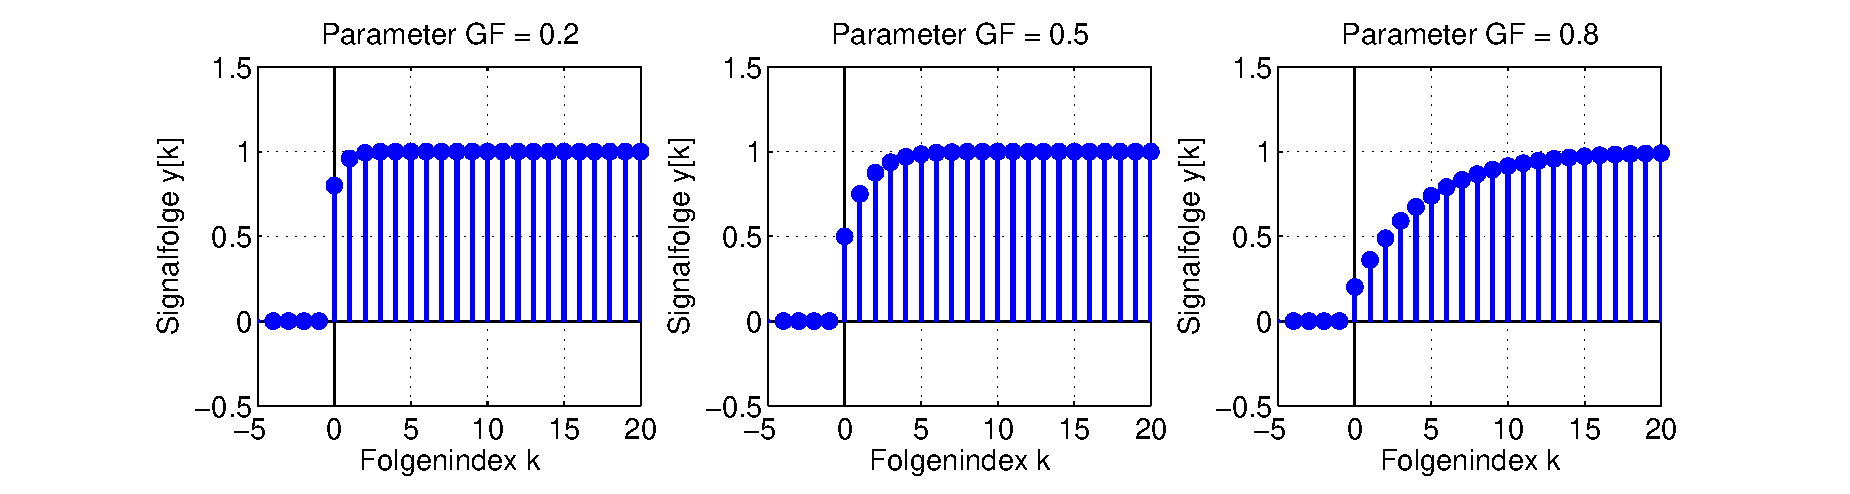
\includegraphics[width=1\textwidth]{Kapitel4/Bilder/image1}}
  \caption{Grafische Darstellung der Wahrscheinlichkeitsverteilung f(x) und Verteilungsfunktion F(x) f\"{u}r die Augenzahl beim W\"{u}rfeln mit zwei W\"{u}rfeln }
  \label{fig:Diskret_Wuerfelexperiment}
\end{figure}

\noindent Zum Beispiel ist f\"{u}r das W\"{u}rfeln die Wahrscheinlichkeit f\"{u}r einen Zahlenwert 3 $\mathrm{<}$ x $\leq$ 7 

\begin{equation}\label{eq:foursix}
P\left(3<x\le 7\right)=\sum _{x_{n} >3}^{7}f\left(x_{n} \right) =\dfrac{3}{36} +\dfrac{4}{36} +\dfrac{5}{36} +\dfrac{6}{36} =\dfrac{18}{36} =\dfrac{1}{2}
\end{equation}

\noindent Sie kann aber auch aus der Verteilungsfunktion berechnet werden. 

\begin{equation}\label{eq:fourseven}
P\left(3<x\le 7\right)=F\left(7\right)-F\left(3\right)=\dfrac{21}{36} -\dfrac{3}{36} =\dfrac{1}{2}
\end{equation}


\noindent Die Werte x$_{n}$, an denen die diskrete Zufallsvariable x eine positive Wahrscheinlichkeit besitzt, werden als m\"{o}gliche Werte von x bezeichnet. In jedem Intervall, in dem kein m\"{o}glicher Wert von x liegt, bleibt die Verteilungsfunktion F(x) konstant. F(x) ist also eine Funktion, die an den Stellen x = x$_{n}$ um die Wahrscheinlichkeit P$_{n}$ = f(x$_{n}$) springt und ansonsten konstant bleibt. F\"{u}r Werte der Zufallsvariable x, die kleiner als der kleinste m\"{o}gliche Wert x$_{min}$ sind, gilt

\begin{equation}\label{eq:foureight}
F(x<x_{\min })=0
\end{equation}

\noindent F\"{u}r den gr\"{o}{\ss}ten vorkommenden Wert x${}_{max}$ nimmt die Verteilungsfunktion den Wert 

\begin{equation}\label{eq:fournine}
F(x\ge x_{\max })=1
\end{equation}

\noindent an. Der Informationsgehalt der Wahrscheinlichkeitsverteilung f(x) und der Verteilungsfunktion F(x) sind identisch. Nach Gleichung \eqref{eq:fourfive} gilt f\"{u}r zwei Zufallsvariablen mit dem Abstand d 

\begin{equation}\label{eq:fourten}
F\left(x\right)=\sum _{x_{n} =-\infty }^{x}f\left(x_{n} \right)
\end{equation}

\noindent und

\begin{equation}\label{eq:foureleven}
F(x-d)=\sum _{x_{n} =-\infty }^{x-d}f(x_{n})
\end{equation}

\noindent Damit kann die Wahrscheinlichkeitsverteilung f(x) bestimmt werden aus der Differenz

\begin{equation}\label{eq:fourtwelve}
f\left(x\right)=F\left(x\right)-F\left(x-d\right)
\end{equation}

\noindent Die Darstellungen k\"{o}nnen also mithilfe dieser Gleichungen ineinander \"{u}berf\"{u}hrt werden. Obwohl beide Funktionen denselben Informationsgehalt haben, ist die Wahrscheinlichkeitsverteilung f(x) f\"{u}r diskrete Verteilungen die anschaulichere Darstellung. Im Gegensatz dazu muss bei Rechnungen mit stetigen Verteilungen die Verteilungsfunktion F(x) verwendet werden, weshalb beide Formen der Darstellung ihre Berechtigung haben.\newline

\noindent Die Wahrscheinlichkeitsverteilung f(x) und die Verteilungsfunktion F(x) sind vergleichbar mit den Darstellungen zur relativen H\"{a}ufigkeit h(x) und der relativen Summenh\"{a}ufigkeit H(x) in der beschreibenden Statistik. Allerdings liegt bei der beschreibenden Statistik eine konkrete Stichprobe vor, w\"{a}hrend die Wahrscheinlichkeitsverteilung f(x) und die Verteilungsfunktion F(x) die Grundgesamtheit eines Wahrscheinlichkeitsexperimentes charakterisieren. 


\subsubsection{Stetige Zufallsvariablen und Verteilungen}

\noindent Eine Zufallsvariable x ist stetig, wenn die zugeh\"{o}rige Verteilungsfunktion F(x) in Integralform dargestellt werden kann.

\begin{equation}\label{eq:fourthirteen}
P(\xi \le x)=F(x)=\int _{-\infty }^{x}f(\xi)d\xi
\end{equation}

\noindent Da in Gleichung \eqref{eq:fourthirteen}die obere Grenze des Integrals der Wert x ist, wird die Integrationsvariable mit dem griechischen $\xi$ bezeichnet. Der Integrand ist eine positive Funktion, die stetig ist oder einzelne Spr\"{u}nge aufweist. Dadurch ist die Verteilungsfunktion F(x) stetig. Der Integrand f(x) hei{\ss}t Wahrscheinlichkeitsdichte der Zufallsvariable x. Aus Gleichung \eqref{eq:fourthirteen}folgt durch Differentiation

\begin{equation}\label{eq:fourfourteen}
f(x)=\dfrac{dF}{dx}
\end{equation}

\noindent Die Wahrscheinlichkeitsdichte f(x) ist demnach die Ableitung der Verteilungsfunktion F(x). Auch bei stetigen Verteilungen ist der Informationsgehalt identisch, sie lassen sich mit den Gleichungen \eqref{eq:fourthirteen} und \eqref{eq:fourfourteen} ineinander umrechnen. Da das Ereignis - $\infty$ $\mathrm{<}$ x $\leq$ $\infty$ ein sicheres Ereignis ist, ergibt sich

\begin{equation}\label{eq:fourfifteen}
P\left(-\infty <x\le \infty \right)=F(\infty)=\int\limits _{-\infty }^{\infty }f(x)dx =1
\end{equation}

\noindent Weiterhin gilt f\"{u}r das Ereignis a $\mathrm{<}$ x $\leq$ b analog zur Gleichung \eqref{eq:fourfour}

\begin{equation}\label{eq:foursixteen}
P\left(a<x\le b\right)=F(b)-F(a)=\int\limits _{a}^{b}f(x)dx
\end{equation}

\noindent Die Wahrscheinlichkeit des Ereignisses a $\mathrm{<}$ x $\leq$ b entspricht der Fl\"{a}che unter der Kurve der Wahrscheinlichkeitsdichte f(x) zwischen den Punkten x = a und x = b. Bild \ref{fig:WahrscheinlichkeitVariableIntervall} stellt diesen Zusammenhang grafisch dar. 

\noindent 
\begin{figure}[H]
  \centerline{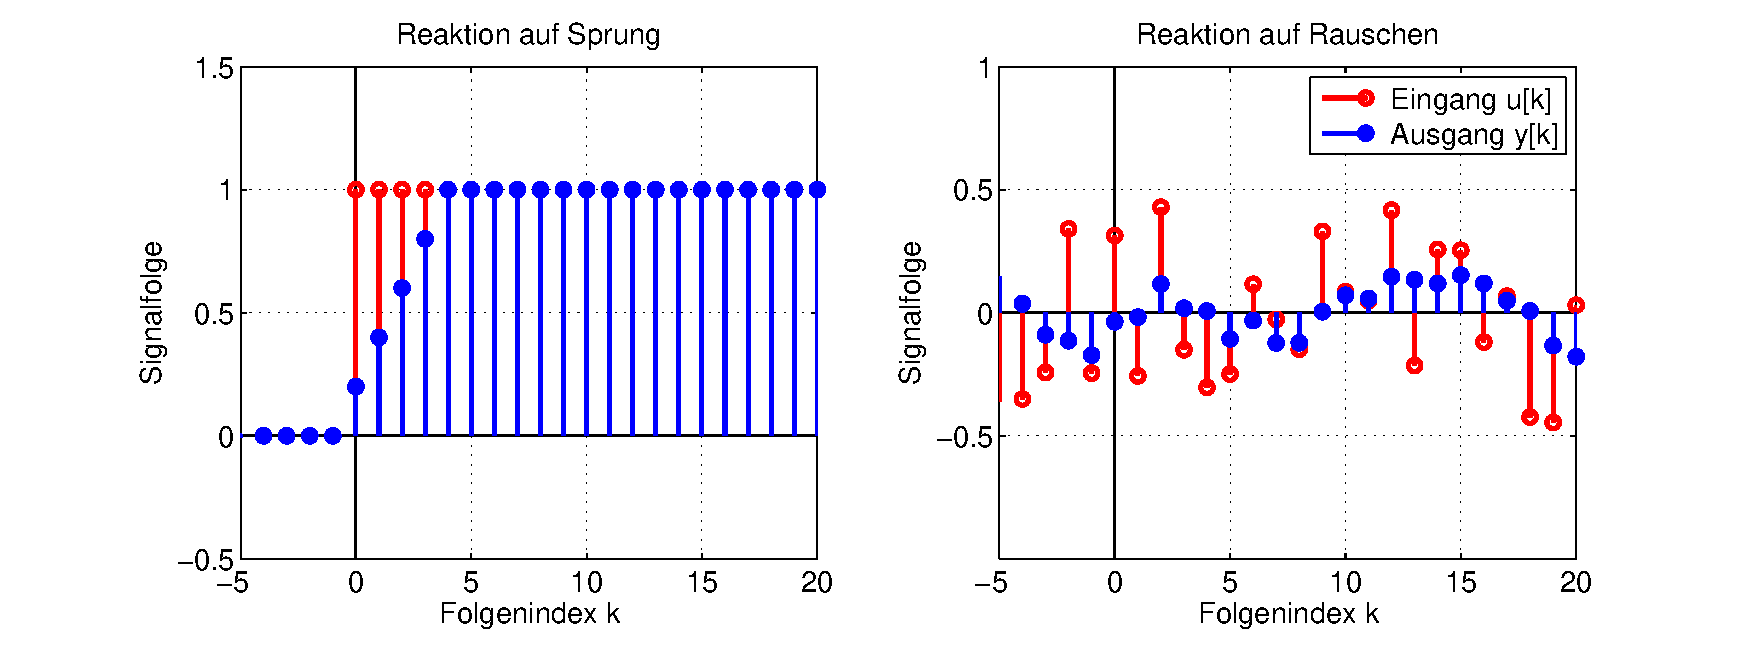
\includegraphics[width=0.5\textwidth]{Kapitel4/Bilder/image2}}
  \caption{Grafische Darstellung der Wahrscheinlichkeit P(a $\mathrm{<}$ x $\mathrm{\le}$ b)}
  \label{fig:WahrscheinlichkeitVariableIntervall}
\end{figure}

\clearpage 

\noindent F\"{u}r ein singul\"{a}res Ereignis x = a ist die Abszisse unendlich klein. Damit wird auch die Fl\"{a}che unter der Kurve unendlich klein und die Wahrscheinlichkeit f\"{u}r den Wert x = a ist 

\begin{equation}\label{eq:fourseventeen}
P(x=a)=0
\end{equation}

\noindent Das bedeutet nicht, dass x = a ein unm\"{o}gliches Ergebnis ist, sondern dass die Wahrscheinlichkeit unendlich klein ist, bei einer stetigen Zufallsvariablen genau einen definierten Wert zu erzielen.\bigskip

\noindent
\colorbox{lightgray}{%
\arrayrulecolor{white}%
\renewcommand\arraystretch{0.6}%
\begin{tabular}{ wl{16.5cm} }
{\fontfamily{phv}\selectfont{Beispiel: Gl\"{u}cksrad}}
\end{tabular}%
}\medskip 

\noindent Ein Gl\"{u}cksrad, das einen beliebigen Winkel x zwischen 0 und 2$.\pi$ einnehmen kann, kann als Zufallsexperiment aufgefasst werden. Alle Winkel x sind gleich wahrscheinlich, deshalb ist die Wahrscheinlichkeitsdichte f(x) konstant P${}_{0}$. Das sichere Ereignis ist, dass der Winkel x in dem Intervall 0 $\mathrm{<}$ x $\leq$ 2$.\pi$ liegt. Es gilt:

\begin{equation}\label{eq:foureighteen}
F(2\cdot \pi )=\int\limits _{0}^{2\cdot \pi }f(x)dx =\int\limits _{0}^{2\cdot \pi }f_{0} dx =2\cdot \pi \cdot f_{0} =1
\end{equation}

\noindent Daraus ergibt sich durch Aufl\"{o}sen nach P$_{0}$ f$_{0}$ die Wahrscheinlichkeitsdichte in dem Bereich 0 $\mathrm{<}$ x $\leq$ 2$.\pi$ von

\begin{equation}\label{eq:fournineteen}
f(x)=f_{0} =\dfrac{1}{2\cdot \pi} 
\end{equation}

\noindent und die Verteilungsfunktion

\begin{equation}\label{eq:fourtwenty}
F(x)=\int\limits _{0}^{x}\dfrac{1}{2\cdot \pi } d\xi  =\dfrac{x}{2\cdot \pi}
\end{equation}

\noindent Bild \ref{fig:Gleichverteilung} stellt die Wahrscheinlichkeitsdichte f(x) und die Verteilungsfunktion F(x) f\"{u}r das Experiment dar.

\noindent 
\begin{figure}[H]
  \centerline{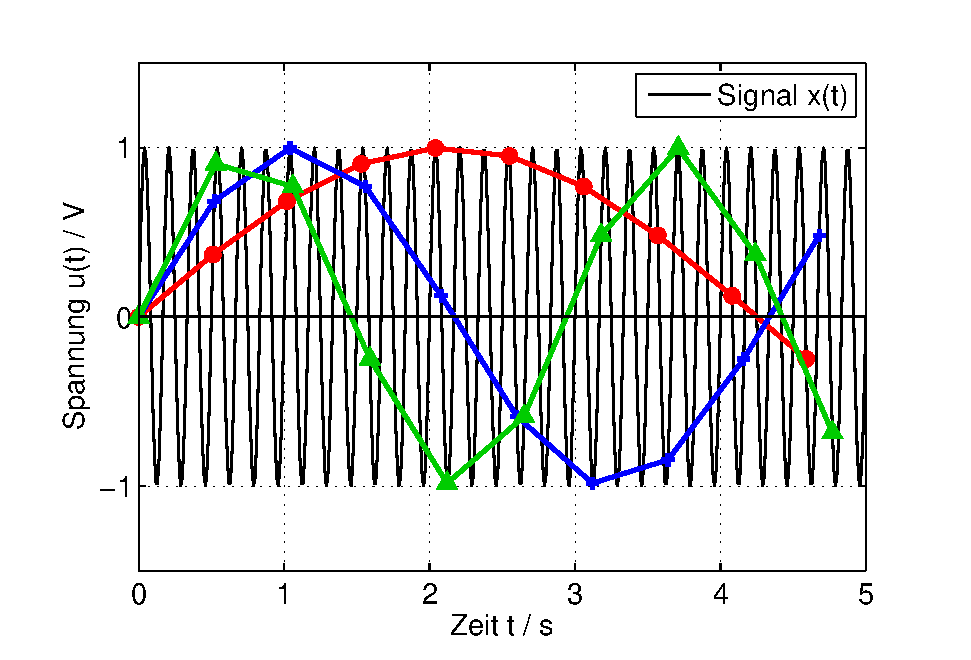
\includegraphics[width=1\textwidth]{Kapitel4/Bilder/image3}}
  \caption{Grafische Darstellung der Wahrscheinlichkeitsdichte f(x) und Verteilungsfunktion F(x) f\"{u}r das Gl\"{u}cksrad-Experiment}
  \label{fig:Gleichverteilung}
\end{figure}

\clearpage

\noindent Die Wahrscheinlichkeit, dass das Gl\"{u}cksrad mit einem Winkel in dem Bereich von a $\mathrm{<}$ x $\leq$ b stehen bleibt, ist 

\begin{equation}\label{eq:fourtwentyone}
P\left(a<x\le b\right)=\int\limits _{a}^{b}\dfrac{1}{2\cdot \pi } dx= \dfrac{b-a}{2\cdot \pi}
\end{equation}

\noindent Alle Ereignisse in dem definierten Intervall zwischen a und b sind gleich wahrscheinlich.

\subsubsection{Nomenklatur f\"{u}r diskrete und stetige Zufallsvariablen}

\noindent Diskrete und stetige Verteilungen werden mit den Funktionen f(x) und F(x) beschrieben. Die Funktion F(x) wird in beiden F\"{a}llen als Verteilungsfunktion bezeichnet. Bei diskreten Zufallsvariablen ist f(x) die Wahrscheinlichkeitsverteilung, bei stetigen Zufallsvariablen ist f(x) die Wahrscheinlichkeitsdichte. Bei Stichproben wird von relativen H\"{a}ufigkeitsverteilungen h(x) und relativen Summenh\"{a}ufigkeiten H(x) gesprochen. Damit ergeben sich die in Tabelle \ref{tab:fourthree} zusammengefassten Bezeichnungen.

\begin{table}[H]
\setlength{\arrayrulewidth}{.1em}
\caption{ Zusammenfassung der Nomenklatur f\"{u}r Stichproben sowie diskrete und stetige Zufallsvariablen}
\setlength{\fboxsep}{0pt}%
\colorbox{lightgray}{%
\arrayrulecolor{white}%
\begin{tabular}{| c | c | c |}
\hline
\parbox[c][0.3in][c]{1.9in}{\smallskip\centering\textbf{\fontfamily{phv}\selectfont{Stichprobe}}} &
\parbox[c][0.3in][c]{2.2in}{\smallskip\centering\textbf{\fontfamily{phv}\selectfont{Diskreter Zufallsprozess}}} &
\parbox[c][0.3in][c]{2.2in}{\smallskip\centering\textbf{\fontfamily{phv}\selectfont{Stetiger Zufallsprozess}}}\\ \hline

\parbox[c][0.5in][c]{1.9in}{\centering\fontfamily{phv}\selectfont{Relative Häufigkeitsverteilung h(x)}} & 
\parbox[c][0.5in][c]{2.2in}{\centering\fontfamily{phv}\selectfont{Wahrscheinlichkeitsverteilung f(x)}} &
\parbox[c][0.5in][c]{2.2in}{\centering\fontfamily{phv}\selectfont{Wahrscheinlichkeitsdichte f(x)}}\\
\hline

\parbox[c][0.5in][c]{1.9in}{\centering\fontfamily{phv}\selectfont{Relative Summenhäufigkeit H(x)}} & 
\parbox[c][0.5in][c]{2.2in}{\centering\fontfamily{phv}\selectfont{Verteilungsfunktion F(x)}} &
\parbox[c][0.5in][c]{2.2in}{\centering\fontfamily{phv}\selectfont{Verteilungsfunktion F(x)}}\\
\hline

\end{tabular}%
}
\label{tab:fourthree}
\end{table}
\noindent 

\clearpage

\subsection{Erwartungswerte von Verteilungen}

\noindent Der Erwartungswert E(x) der Zufallsvariablen x entspricht dem Wert, der sich bei oftmaligem Wiederholen des zugrunde liegenden Zufallsexperiments im Mittel einstellt. Durch den Erwartungswert E(x) wird sp\"{a}ter die Lage der vorliegenden Verteilung beschrieben. Der Erwartungswert kann aber nicht nur von der Zufallsvariablen x bestimmt werden, sondern auch von Funktionen von Zufallsvariablen g(x). Der Erwartungswert eignet sich damit zur Bestimmung von Kenngr\"{o}{\ss}en einer Verteilung. Dieser Zusammenhang wird in Abschnitten \ref{fourthree} gezeigt.


\subsubsection{Definition des Erwartungswert-Operators}

\noindent F\"{u}r eine beliebige Zufallsvariable x und eine f\"{u}r alle Werte von x definierte reellwertige Funktion y = g(x) der Zufallsvariablen x wird der Ausdruck 

\begin{equation}\label{eq:fourtwentytwo}
E(y)=E\left(g(x)\right)=\sum _{x_{n} =-\infty }^{\infty }\left(g(x_{n})\cdot f(x_{n})\right)
\end{equation}

\noindent beziehungsweise 

\begin{equation}\label{eq:fourtwentythree}
E(y)=E\left(g(x)\right)=\int\limits _{-\infty}^{\infty}g(x)\cdot f(x)dx
\end{equation}

\noindent als mathematischer Erwartungswert der Funktion g(x) oder als Erwartung von g(x) bezeichnet. Dabei wird die Konvergenz der Summe beziehungsweise des Integrals vorausgesetzt.\bigskip

\noindent
\colorbox{lightgray}{%
\arrayrulecolor{white}%
\renewcommand\arraystretch{0.6}%
\begin{tabular}{ wl{16.5cm} }
{\fontfamily{phv}\selectfont{Beispiel:Gl\"{u}cksspiel mit W\"{u}rfeln}}
\end{tabular}%
}\medskip 

\noindent Zwei Personen A und B spielen das folgende Spiel: A w\"{u}rfelt mit einem regelm\"{a}{\ss}igen W\"{u}rfel und erh\"{a}lt von B

\begin{itemize}
    \item 10 Cent f\"{u}r eine Eins oder Zwei,
    \item 20 Cent f\"{u}r eine Drei oder Vier,
    \item 40 Cent f\"{u}r eine F\"{u}nf und
    \item 80 Cent f\"{u}r eine Sechs.
\end{itemize}

\noindent Spieler A soll an Spieler B vor jedem Spiel einen Betrag von 50 Cent zahlen. Um zu \"{u}berpr\"{u}fen, ob Spieler A bei mehreren Spielen einen Gewinn erzielt, muss die durchschnittliche Gewinnerwartung pro Spiel berechnet werden. Die durchschnittliche Gewinnerwartung ergibt sich aus der Wahrscheinlichkeit, eine bestimmte Zahl zu w\"{u}rfeln, und dem zugeordneten Gewinn. Zum Beispiel betr\"{a}gt die Wahrscheinlichkeit, eine Eins zu w\"{u}rfeln, 1/6, und der zugeh\"{o}rige Gewinn betr\"{a}gt 10 Cent. 

\noindent Zur Berechnung wird eine Zufallsvariable x definiert, die die beim Wurf des W\"{u}rfels erzielte Augenzahl darstellt. In Tabelle \ref{tab:fourfour} ist jedem m\"{o}glichen Wert der Zufallsvariablen x der Gewinn von A zugeordnet. Er bildet die Funktion g(x).

\begin{table}[H]
\setlength{\arrayrulewidth}{.1em}
\caption{Zuordnung des Gewinns g(x) zur Zufallsvariablen x}
\setlength{\fboxsep}{0pt}%
\colorbox{lightgray}{%
\arrayrulecolor{white}%
\begin{tabular}{| wc{2cm} | wc{2cm} | wc{2cm} | wc{2cm} | wc{2cm} | wc{2cm} | wc{2cm} }
\hline\xrowht{15pt}

\fontfamily{phv}\selectfont{x} & 1 & 2 & 3 & 4 & 5 & 6 \\ \hline \xrowht{25pt}

\fontfamily{phv}\selectfont{(x)} & 10 & 10 & 20 & 20 & 40 & 80\\ \hline

\end{tabular}%
}
\label{tab:fourfour}
\end{table}

\noindent Da die Werte von x vom Zufall abh\"{a}ngen, gilt dies auch f\"{u}r den Wert, den g(x) bei einem Spiel jeweils annimmt. Die Funktion g(x) der Zufallsvariable x ist also selbst eine Zufallsvariable y = g(x). In diesem Beispiel betr\"{a}gt die durchschnittliche Gewinnerwartung

\begin{equation}\label{eq:fourtwentyfour}
E(y)=E(g(x))=\sum _{x_{n} =1}^{6}\left(g(x_{n})\cdot f(x_{n})\right) =10\cdot \dfrac{1}{6} +10\cdot \dfrac{1}{6} +20\cdot \dfrac{1}{6} +20\cdot \dfrac{1}{6} +40\cdot \dfrac{1}{6} +80\cdot \dfrac{1}{6} =30
\end{equation}

\noindent Die durchschnittliche Gewinnerwartung pro Spiel ist mit 30 Cent geringer als der Spieleinsatz von 50 Cent. Spieler A wird bei mehreren Spieldurchg\"{a}ngen demnach Geld verlieren.

\subsubsection{Eigenschaften des Erwartungswert-Operators}

\noindent Es gibt einige Eigenschaften des Erwartungswert-Operators, die dazu verwendet werden k\"{o}nnen, den Erwartungswert von Funktionen von Zufallsvariablen zu bestimmen. Da der Erwartungswert f\"{u}r stetige Zufallsgr\"{o}{\ss}en \"{u}ber ein Integral definiert ist, ergeben sich die Eigenschaften des Erwartungswert-Operators aus den Eigenschaften der Integralrechnung. Im Folgenden werden Rechenregeln f\"{u}r den Erwartungswert stetiger Zufallsvariablen hergeleitet. Dieselben Rechenregeln gelten auch f\"{u}r diskrete Zufallsvariablen.\bigskip

{\fontfamily{phv}\selectfont
\noindent\textbf{Erwartungswert einer Konstanten}}\smallskip

\noindent Der Erwartungswert einer konstanten Gr\"{o}{\ss}e k besitzt den Wert k, denn es gilt:

\begin{equation}\label{eq:fourtwentyfive}
E(k)=\int\limits _{-\infty }^{\infty }k \cdot f(x)dx=k\cdot \int\limits _{-\infty }^{\infty }f(x) dx =k\cdot 1=k
\end{equation}

{\fontfamily{phv}\selectfont
\noindent\textbf{Linearit\"{a}t des Erwartungswert-Operators}}\smallskip

\noindent Der Erwartungswert ist ein linearer Operator. F\"{u}r die Zufallsvariable 

\begin{equation}\label{eq:fourtwentysix}
y=a\cdot h(x)+b\cdot g(x)
\end{equation}

\noindent wird der Erwartungswert berechnet aus

\begin{equation}\label{eq:fourtwentyseven}
\begin{split}
E(y) & = E\left(a\cdot h(x)+b\cdot g(x)\right)=\int\limits _{-\infty }^{\infty }(a\cdot h(x)+b\cdot g(x)) \cdot f(x)dx \\
& = a\cdot \int\limits _{-\infty }^{\infty }h(x) \cdot f(x)dx+b\cdot \int\limits _{-\infty }^{\infty }g(x) \cdot f(x)dx=a\cdot E(h(x))+b\cdot E(g(x))  
\end{split}
\end{equation}

\noindent Ein Sonderfall ist die lineare Transformation der Form 

\begin{equation}\label{eq:fourtwentyeight}
y=a\cdot x+b
\end{equation}

\noindent Aufgrund der Linearit\"{a}t des Erwartungswertes ergibt sich 

\begin{equation}\label{eq:fourtwentynine}
E(y)=E(a\cdot x+b)=a\cdot E(x)+b
\end{equation}

\noindent Ein Vergleich der Gleichungen \eqref{eq:fourtwentyeight} und \eqref{eq:fourtwentynine} zeigt, dass sich der Erwartungswert analog zur Zufallsvariable verschiebt. \bigskip

{\fontfamily{phv}\selectfont
\noindent\textbf{Erwartungswert symmetrischer Verteilungen}}\smallskip

\noindent F\"{u}r Ist eine zum Punkt c symmetrische Verteilung f(x) symmetrisch zum Punkt c

\begin{equation}\label{eq:fourthirty}
f(c-x)=f(c+x)
\end{equation}

\noindent gilt f\"{u}r den soll der Erwartungswert-Operator

\begin{equation}\label{eq:fourthirtyone}
E(x)=\int\limits _{-\infty }^{\infty }x\cdot f(x)dx =\int\limits _{-\infty }^{c}x\cdot f(x)dx +\int\limits _{c}^{\infty }x\cdot f(x)dx
\end{equation}

\noindent berechnet werden. Durch die Substitution x = c - $\xi$ beziehungsweise x = c + $\xi$ ergibt sich

\begin{equation}\label{eq:fourthirtytwo}
E(x)=\int\limits _{0}^{\infty }(c-\xi )\cdot f(c-\xi )d\xi  +\int\limits _{0}^{\infty }(c+\xi )\cdot f(c+\xi )d\xi
\end{equation}

\noindent Wegen der identischen Integrationsgrenzen k\"{o}nnen die Integrale zusammengefasst werden.

\begin{equation}\label{eq:fourthirtythree}
\begin{split}
E(x) & = \int\limits _{0}^{\infty }c\cdot f(c-\xi)d\xi  +\int\limits _{0}^{\infty }c\cdot f(c+\xi)d\xi  -\int\limits _{0}^{\infty }\xi \cdot f(c-\xi )d\xi  +\int\limits _{0}^{\infty }\xi \cdot f(c+\xi)d\xi\\
& =  \int\limits _{-\infty}^{\infty }c\cdot f(c-\xi)d\xi - \int\limits _{0}^{\infty }\xi\cdot (f(c-\xi)  -  f(c+\xi ))d\xi
\end{split}
\end{equation}

\noindent Der erste Summand ist der Erwartungswert einer konstanten Gr\"{o}{\ss}e c. Der zweite Summand besteht aus einer Differenz von Wahrscheinlichkeitsdichten. Da die Wahrscheinlichkeitsdichte symmetrisch ist, ist die Differenz null. Damit ergibt sich der Erwartungswert einer symmetrischen Verteilung zu

\begin{equation}\label{eq:fourthirtyfour}
E(x)=c\cdot \int\limits _{-\infty }^{\infty }f\left(c-\xi \right) d\xi  -0=c
\end{equation}

\clearpage

{\fontfamily{phv}\selectfont
\noindent\textbf{Zusammenfassung}}\smallskip

\noindent In Tabelle \ref{tab:fourfive} werden die Eigenschaften des Erwartungswert-Operators zusammengefasst. Das Rechnen mit Erwartungswerten ist insbesondere bei der Herleitung von Gesetzm\"{a}{\ss}igkeiten f\"{u}r die Grundgesamtheit und die Berechnung der Erwartungstreue bei Sch\"{a}tzungen von Bedeutung.

\begin{table}[H]
\setlength{\arrayrulewidth}{.1em}
\caption{Zusammenfassung der Eigenschaften des Erwartungswert-Operators}
\setlength{\fboxsep}{0pt}%
\colorbox{lightgray}{%
\arrayrulecolor{white}%
\begin{tabular}{| c | c |}
\hline
\parbox[c][0.35in][c]{2.5in}{\smallskip\centering\textbf{\fontfamily{phv}\selectfont{Rechenoperation}}} & \parbox[c][0.35in][c]{4.2in}{\smallskip\centering\textbf{\fontfamily{phv}\selectfont{Eigenschaften des Erwartungswert-Operators}}}\\ \hline

\parbox[c][1.6in][c]{2.5in}{\centering\fontfamily{phv}\selectfont{Definition Erwartungswert}} & 
\parbox[c][1.6in][c]{4.2in}{\centering\fontfamily{phv}\selectfont{$E\left(y\right)=E(g(x))=\sum _{x_{n} =-\infty }^{\infty }\left(g(x_{n} )\cdot f(x_{n} )\right) $\bigskip

beziehungsweise\bigskip

$E(y)=E(g(x))=\int\limits _{-\infty }^{\infty }g(x)\cdot f(x)dx$}}\\ \hline

\parbox[c][0.4in][c]{2.5in}{\centering{\fontfamily{phv}\selectfont{Erwartungswert einer Konstanten}}} & 
\parbox[c][0.4in][c]{4.2in}{\centering{$E\left(k\right)=k$}}\\ \hline

\parbox[c][0.4in][c]{2.5in}{\centering{\fontfamily{phv}\selectfont{Linearität}}} & 
\parbox[c][0.4in][c]{4.2in}{\centering{$E(a\cdot h(x)+b\cdot g(x))=a\cdot E(h(x))+b\cdot E(g(x))$}}\\ \hline

\parbox[c][0.4in][c]{2.5in}{\centering{\fontfamily{phv}\selectfont{Lineare Transformation}}} & 
\parbox[c][0.4in][c]{4.2in}{\centering{$E(y)=E(a\cdot x+b)=a\cdot E(x)+b$}}\\ \hline

\parbox[c][0.4in][c]{2.5in}{\centering{\fontfamily{phv}\selectfont{Symmetrie f(c -- x) = f(x -- c)}}} & 
\parbox[c][0.4in][c]{4.2in}{\centering{$E(x)=c$}}\\ \hline

\end{tabular}%
}
\label{tab:fourfive}
\end{table}

\clearpage

\subsection{Kennwerte von Verteilungen}

\noindent Bei der beschreibenden Statistik werden vorliegende Daten aus Stichproben analysiert. Dabei werden f\"{u}r die konkreten Daten H\"{a}ufigkeitsverteilungen bestimmt sowie empirische Kenngr\"{o}{\ss}en f\"{u}r die Lage, die Streuung und die Symmetrie berechnet. Diese Kenngr\"{o}{\ss}en lassen sich auch f\"{u}r Verteilungen Zufallsvariablen mit einer bekannten Wahrscheinlichkeitsverteilung berechnen. Im Gegensatz zur deskriptiven Statistik werden bei der Wahrscheinlichkeitsrechnung alle theoretisch m\"{o}glichen Werte der Zufallsvariablen ausgewertet. Deshalb werden die Kennwerte auch als theoretische Kennwerte bezeichnet.

\subsubsection{Momente und Zentralmomente einer Verteilung}

\noindent Kennwerte von Verteilungen k\"{o}nnen als Moment beziehungsweise als Zentralmoment der Ordnung k berechnet werden. Das k-te Moment einer Verteilung oder der Zufallsvariable x ist definiert als der Erwartungswert der Funktion 

\begin{equation}\label{eq:fourthirtyfive}
g(x)=x^{k}
\end{equation}

\noindent F\"{u}r diskrete Verteilungen ergibt sich 

\begin{equation}\label{eq:fourthirtysix}
E(x^{k})=\sum _{x_{n} =-\infty }^{\infty }\left(x_{n}^{k} \cdot f(x_{n})\right)
\end{equation}

\noindent und f\"{u}r stetige Verteilungen berechnet sich das k-te Moment zu

\begin{equation}\label{eq:fourthirtyseven}
E(x^{k})=\int\limits _{-\infty }^{\infty }x^{k} \cdot f(x) dx
\end{equation}

\noindent Der Erwartungswert der Funktion 

\begin{equation}\label{eq:fourthirtyeight}
g(x)=(x-\mu)^{k}
\end{equation}

\noindent f\"{u}hrt zu dem k-ten Zentralmoment. Dabei ist µ der arithmetische Mittelwert der Verteilung, auf ihn wird in Abschnitt 4.3.2 detailliert eingegangen. F\"{u}r diskrete Verteilungen berechnet sich das k-te Zentralmoment aus 

\begin{equation}\label{eq:fourthirtynine}
E\left((x-\mu)^{k} \right)=\sum _{x_{n} =-\infty }^{\infty }\left((x_{n} -\mu)^{k} \cdot f(x_{n} )\right)
\end{equation}

\noindent und f\"{u}r stetige Verteilungen aus

\begin{equation}\label{eq:fourfourty}
E\left((x-\mu)^{k} \right)=\int\limits _{-\infty }^{\infty }\left(x-\mu \right)^{k} \cdot f(x)dx
\end{equation}

\noindent Aufgrund der Linearit\"{a}t des Erwartungswertes kann die Berechnung des Zentralmomentes auf die Berechnung des Momentes zur\"{u}ckgef\"{u}hrt werden. Zum Beispiel ergibt sich f\"{u}r das zweite Zentralmoment 

\begin{equation}\label{eq:fourfourtyone}
\begin{split}
E\left(\left(x-\mu \right)^{2} \right) & = E\left(x^{2} -2\cdot \mu \cdot x+\mu ^{2} \right)=E\left(x^{2} \right)-2\cdot \mu \cdot E\left(x\right)+\mu ^{2}\\
& = E(x^{2}) -2\cdot\mu ^{2} +\mu ^{2} = E(x^{2})-\mu ^{2}
\end{split}
\end{equation}

\noindent Entsprechend k\"{o}nnen h\"{o}here Zentralmomente umgeformt werden. F\"{u}r das dritte Zentralmoment ergibt sich mit den Rechenregeln des Erwartungswertes 

\begin{equation}\label{eq:fourfourtytwo}
E\left((x-\mu )^{3} \right)=E(x^{3} )-3\cdot \mu \cdot E(x^{2})+2\cdot \mu ^{3}
\end{equation}

\subsubsection{Lagekennwerte einer Verteilung}

\noindent Wie bei der deskriptiven Statistik k\"{o}nnen f\"{u}r Wahrscheinlichkeitsverteilungen Lagekennwerte angegeben werden. In Anlehnung an die beschreibende Statistik werden in diesem Abschnitt der arithmetische Mittelwert und der Median einer Verteilung eingef\"{u}hrt.

{\fontfamily{phv}\selectfont
\noindent\textbf{Arithmetischer Mittelwert einer Verteilung}}\smallskip

\noindent Der theoretisch erwartete Mittelwert einer Verteilung wird mit µ bezeichnet. Er berechnet sich bei einer diskreten Verteilung zu

\begin{equation}\label{eq:fourfourtythree}
\mu =\sum _{x_{n} =-\infty }^{\infty }\left(x_{n} \cdot f\left(x_{n} \right)\right)
\end{equation}

\noindent und bei einer stetigen Verteilung zu

\begin{equation}\label{eq:fourfourtyfour}
\mu =\int\limits _{-\infty }^{\infty }x\cdot f(x)dx
\end{equation}

\noindent Der Mittelwert kann auch als Erwartungswert eines Momentes erster Ordnung dargestellt werden. 

\begin{equation}\label{eq:fourfourtyfive}
\mu =E(x^{1})=E(x)
\end{equation}

\noindent Der Mittelwert der Verteilung wird auch als Mittelwert der Zufallsvariable x oder Erwartungswert von x bezeichnet. Bei der Berechnung des Mittelwertes wird vorausgesetzt, dass die Summe \eqref{eq:fourfourtythree} beziehungsweise das Integral \eqref{eq:fourfourtyfour} konvergieren, was aber in praktischen F\"{a}llen immer gegeben ist.\bigskip

{\fontfamily{phv}\selectfont
\noindent\textbf{Median einer Verteilung}}\smallskip

\noindent Der Median einer Verteilung ergibt sich aus der Bedingung

\begin{equation}\label{eq:fourfourtysix}
F\left(x_{MED} \right)=0.5
\end{equation}

\noindent Im Fall einer stetigen Zufallsvariable x ist in praktischen F\"{a}llen auch die Verteilungsfunktion F(x) stetig. Damit kann der Median analytisch oder zumindest numerisch bestimmt werden. Im Fall einer diskreten Zufallsvariable x muss der Median mit vergleichbaren Verfahren wie bei der deskriptiven Statistik bestimmt werden.

\clearpage

\noindent
\colorbox{lightgray}{%
\arrayrulecolor{white}%
\renewcommand\arraystretch{0.6}%
\begin{tabular}{ wl{16.5cm} }
{\fontfamily{phv}\selectfont{Beispiel: W\"{u}rfeln mit zwei W\"{u}rfeln}}
\end{tabular}%
}\medskip  

\noindent Bei dem Beispiel des W\"{u}rfelns mit zwei W\"{u}rfeln ergibt sich ein Mittelwert von 

\begin{equation}\label{eq:fourfourtyseven}
\mu =\sum _{x_{n} =-\infty }^{\infty }\left(x_{n} \cdot f(x_{n} )\right) =7
\end{equation}

\noindent Der Median errechnet sich nach den Darstellungen zur deskriptiven Statistik aus

\begin{equation}\label{eq:fourfourtyeight}
x_{MED} =c_{n-1} +\dfrac{0.5-F(c_{n-1})}{f(c_{n})} \cdot d=6+\dfrac{0.5-\dfrac{15}{36} }{\dfrac{6}{36} } \cdot 1=6+\dfrac{1}{2} =6.5
\end{equation}

\noindent
\colorbox{lightgray}{%
\arrayrulecolor{white}%
\renewcommand\arraystretch{0.6}%
\begin{tabular}{ wl{16.5cm} }
{\fontfamily{phv}\selectfont{Beispiel: Gl\"{u}cksrad}}
\end{tabular}%
}\medskip 

\noindent Bei dem Beispiel des Gl\"{u}cksrades ergibt sich ein Mittelwert von

\begin{equation}\label{eq:fourfourtynine}
\mu =\int\limits _{0}^{2\cdot \pi }x\cdot f\left(x\right)dx =\int\limits _{0}^{2\cdot \pi}x\cdot \dfrac{1}{2\cdot \pi} dx =\left. \dfrac{1}{2\cdot \pi } \cdot (\dfrac{x^{2}}{2})\right|_{0}^{2\cdot \pi} =\pi
\end{equation}

\noindent Der Median ergibt sich aus Bild \ref{fig:Gleichverteilung} zu

\begin{equation}\label{eq:fourfifty}
x_{MED} =\pi
\end{equation}

\subsubsection{Streuungskennwerte einer Verteilung}

\noindent Analog zu den Lagekennwerten von Verteilungen k\"{o}nnen Streuungskennwerte angegeben werden. In diesem Abschnitt werden die Spannweite, die Varianz und die Quantile einer Verteilung eingef\"{u}hrt.\bigskip

{\fontfamily{phv}\selectfont
\noindent\textbf{Spannweite einer Verteilung}}\smallskip

\noindent Sind die Ereignisse der Verteilung f(x) auf ein Intervall I begrenzt, kann die Spannweite der Verteilung angegeben werden als 

\begin{equation}\label{eq:fourfiftyone}
\Delta x=\max (I)-\min (I)
\end{equation}

{\fontfamily{phv}\selectfont
\noindent\textbf{Varianz und Standardabweichung einer Verteilung}}\smallskip

\noindent Die Varianz einer Verteilung ist ein Ma{\ss} f\"{u}r die theoretisch erwartete Streuung der Werte, die die Zufallsvariable x annehmen kann. Sie wird mit $\sigma^{2}$ bezeichnet und ist \"{u}ber den Erwartungswert des zweiten Zentralmomentes 

\begin{equation}\label{eq:fourfiftytwo}
\sigma ^{2} =E\left((x-\mu)^{2} \right)
\end{equation}

\noindent definiert. Im diskreten Fall berechnet sie sich zu

\begin{equation}\label{eq:fourfiftythree}
\sigma ^{2} =\sum _{x_{n} =-\infty }^{\infty }\left((x_{n} -\mu)^{2} \cdot f(x_{n})\right)
\end{equation}

\noindent und im stetigen Fall zu

\begin{equation}\label{eq:fourfiftyfour}
\sigma ^{2} =\int\limits _{-\infty }^{\infty }\left(x-\mu \right)^{2} \cdot f(x)dx
\end{equation}

\noindent Die Varianz einer Verteilung wird auch als Varianz der Zufallsvariable x bezeichnet. Die Varianz der Verteilung kann mit den Rechenregeln des Erwartungswertes umgeformt werden zu

\begin{equation}\label{eq:fourfiftyfive}
\sigma ^{2} =E\left((x-\mu)^{2} \right)=E\left(x^{2} -2\cdot x\cdot \mu +\mu ^{2} \right)=E(x^{2})-2\cdot \mu \cdot E(x)+\mu ^{2} =E(x^{2})-\mu ^{2}
\end{equation}

\noindent Aus den Definitionsgleichungen ergibt sich, dass die Varianz immer gr\"{o}{\ss}er oder gleich 0 ist. Die positive Wurzel der Varianz wird bei der beschreibenden Statistik als Standardabweichung eingef\"{u}hrt. F\"{u}r diskrete Verteilungen berechnet sich die Standardabweichung $\sigma$ aus 

\begin{equation}\label{eq:fourfiftysix}
\sigma =\sqrt{\sum _{x_{n} =-\infty }^{\infty }\left((x_{n} -\mu)^{2} \cdot f(x_{n})\right)}
\end{equation}

\noindent und f\"{u}r stetige Verteilungen ergibt sich 

\begin{equation}\label{eq:fourfiftyseven}
\sigma =\sqrt{\int\limits _{-\infty }^{\infty }\left(x-\mu \right)^{2} \cdot f(x) dx}
\end{equation}

{\fontfamily{phv}\selectfont
\noindent\textbf{Quantilabst\"{a}nde einer Verteilung}}\smallskip

\noindent Analog zum Median einer Verteilung ergibt sich aus der Bedingung

\begin{equation}\label{eq:fourfiftyeight}
F(x_{P})=P
\end{equation}

\noindent das P-Quantil einer Verteilung. Im Fall einer stetigen Zufallsvariable x ist auch die Verteilungsfunktion F(x) stetig. Damit kann das P-Quantil analytisch oder zumindest numerisch bestimmt werden. Im Fall einer diskreten Zufallsvariable muss das P-Quantil wieder mit vergleichbaren Verfahren bestimmt werden, wie bei der deskriptiven Statistik. Der Quantilabstand berechnet sich dann aus der Differenz zweier Quantile. Der Inter-Quartil-Range berechnet sich zu

\begin{equation}\label{eq:fourfiftynine}
IQR=x_{0.75} -x_{0.25}
\end{equation}

\noindent
\colorbox{lightgray}{%
\arrayrulecolor{white}%
\renewcommand\arraystretch{0.6}%
\begin{tabular}{ wl{16.5cm} }
{\fontfamily{phv}\selectfont{Beispiel: W\"{u}rfeln mit zwei W\"{u}rfeln}}
\end{tabular}%
}\medskip 

\noindent Bei dem Beispiel des W\"{u}rfelns mit zwei W\"{u}rfeln ergibt sich eine Spannweite von 

\begin{equation}\label{eq:foursixty}
\Delta x=\max (I)-\min (I)=12-2=10
\end{equation}

\noindent Die Varianz von

\begin{equation}\label{eq:foursixtyone}
\sigma ^{2} =\sum _{x_{n} =-\infty }^{\infty }\left(\left(x_{n} -\mu \right)^{2} \cdot f(x_{n} )\right) =5.83
\end{equation}

\noindent f\"{u}hrt zu einer Standardabweichung

\begin{equation}\label{eq:foursixtytwo}
\sigma =\sqrt{\sum _{x_{n} =-\infty }^{\infty }\left((x_{n} -\mu)^{2} \cdot f(x_{n})\right) } =\sqrt{5.83} =2.41
\end{equation}

\noindent Der Inter-Quartil-Range errechnet sich zu

\begin{equation}\label{eq:foursixtythree}
IQR=x_{0.75} -x_{0.25} =8.25-4.75=3.5
\end{equation}

\noindent
\colorbox{lightgray}{%
\arrayrulecolor{white}%
\renewcommand\arraystretch{0.6}%
\begin{tabular}{ wl{16.5cm} }
{\fontfamily{phv}\selectfont{Beispiel: Gl\"{u}cksrad}}
\end{tabular}%
}\medskip 

\noindent Bei dem Gl\"{u}cksrad erstreckt sich das Intervall I von 0 bis 2$.\pi$, die Spannweite betr\"{a}gt damit $\Delta$x = 2$.\pi$. Die Varianz betr\"{a}gt

\begin{equation}\label{eq:foursixtyfour}
\sigma ^{2} =\int\limits _{-\infty }^{\infty }(x-\mu)^{2} \cdot f(x)dx =\int\limits _{0}^{2\cdot \pi}(x-\pi)^{2} \cdot \dfrac{1}{2\cdot \pi} dx =\dfrac{1}{3} \cdot \pi ^{2}
\end{equation}

\noindent Damit ergibt sich eine Standardabweichung von 

\begin{equation}\label{eq:foursixtyfive}
\sigma =\sqrt{\int\limits _{-\infty}^{\infty}\left(x-\mu \right)^{2} \cdot f(x)dx} =\sqrt{\int\limits _{0}^{2\cdot \pi}(x-\pi)^{2} \cdot \dfrac{1}{2\cdot \pi} dx} =\dfrac{1}{\sqrt{3}} \cdot \pi
\end{equation}

\noindent Aus Bild \ref{fig:Gleichverteilung} kann der Inter-Quartil-Range bestimmt werden zu

\begin{equation}\label{eq:foursixtysix}
IQR=x_{0.75} -x_{0.25} =\dfrac{3\cdot \pi}{2} -\dfrac{\pi}{2} =\pi
\end{equation}

\subsubsection{Schiefe oder Symmetrie einer Verteilung}

\noindent Nachdem die Begriffe des Momentes und Zentralmomentes einer Verteilung eingef\"{u}hrt sind, wird die Symmetrie einer Verteilung mit dem Momenten- und Quantilkoeffizienten der Schiefe beschrieben. 

{\fontfamily{phv}\selectfont
\noindent\textbf{Momentenkoeffizient der Schiefe}}\smallskip

\noindent Analog zum Momentenkoeffizient der Schiefe in der deskriptiven Statistik wird das dritte normierte zentrale Moment zur Definition der Schiefe $\gamma$ einer Verteilung verwendet: 

\begin{equation}\label{eq:foursixtyseven}
\gamma =\dfrac{1}{\sigma ^{3}} \cdot E\left((x-\mu)^{3} \right)
\end{equation}

{\fontfamily{phv}\selectfont
\noindent\textbf{Quantilkoeffizient der Schiefe}}\smallskip

\noindent Alternativ kann die Symmetrie oder Schiefe einer Verteilung \"{u}ber eine Kenngr\"{o}{\ss}e charakterisiert werden, die die Symmetrie der Quantile der Verteilung bewertet. Dazu wird der Quantilkoeffizient der Schiefe wie bei der deskriptiven Statistik berechnet aus

\begin{equation}\label{eq:foursixtyeight}
g_{P} =\dfrac{(x_{1-P} -x_{MED})-\left(x_{MED} -x_{P} \right)}{x_{1-P} -x_{P}}
\end{equation}

\noindent F\"{u}r P = 25 \% ergibt sich der Quartilkoeffizient zu

\begin{equation}\label{eq:foursixtynine}
g_{0.25} =\dfrac{\left(x_{0.75} -x_{MED} \right)-\left(x_{MED} -x_{0.25} \right)}{x_{0.75} -x_{0.25} }
\end{equation}

\noindent Die Interpretation des Momenten- oder Quantilkoeffizienten der Schiefe erfolgt analog zu den Ausf\"{u}hrungen bei der deskriptiven Statistik.

\begin{table}[H]
\setlength{\arrayrulewidth}{.1em}
\caption{Bewertung des Momentenkoeffizienten der Schiefe}
\setlength{\fboxsep}{0pt}%
\colorbox{lightgray}{%
\arrayrulecolor{white}%
\begin{tabular}{| c | c |}
\hline
\parbox[c][0.3in][c]{3.3in}{\smallskip\centering\textbf{\fontfamily{phv}\selectfont{Kennwert}}} & 
\parbox[c][0.3in][c]{3.3in}{\smallskip\centering\textbf{\fontfamily{phv}\selectfont{Symmetrieeigenschaft}}}\\ \hline


\parbox[c][0.3in][c]{3.3in}{\centering\fontfamily{phv}\selectfont{$g_{P} \mathrm{>} 0$}} & 
\parbox[c][0.3in][c]{3.3in}{\centering\fontfamily{phv}\selectfont{Rechtsschiefe Verteilung}} \\
\hline

\parbox[c][0.3in][c]{3.3in}{\centering\fontfamily{phv}\selectfont{$g_{P}= 0$}} & 
\parbox[c][0.3in][c]{3.3in}{\centering\fontfamily{phv}\selectfont{Symmetrische Verteilung}} \\
\hline

\parbox[c][0.3in][c]{3.3in}{\centering\fontfamily{phv}\selectfont{$g_{P} \mathrm{<} 0$}} & 
\parbox[c][0.3in][c]{3.3in}{\centering\fontfamily{phv}\selectfont{Linksschiefe Verteilung}} \\
\hline

\end{tabular}%
}
\label{tab:foursix}
\end{table}

\noindent
\colorbox{lightgray}{%
\arrayrulecolor{white}%
\renewcommand\arraystretch{0.6}%
\begin{tabular}{ wl{16.5cm} }
{\fontfamily{phv}\selectfont{Beispiel: Schiefe einer Verteilung}}
\end{tabular}%
}\medskip 

\noindent Die Schiefe einer stetigen Verteilung wird an einem Beispiel verdeutlicht.

\begin{equation}\label{eq:fourseventy}
f(x)=\left\{\begin{array}{ll}
{0 \qquad \;\;\; \text{ für } x<0} \\
{x\cdot e^{-x}  \quad \text{für} x\ge 0} \end{array}\right.
\end{equation}

\noindent Bild \ref{fig:SchiefeVerteilung} stellt die Verteilung aus Gleichung \eqref{eq:fourseventy} dar.

\begin{figure}[H]
  \centerline{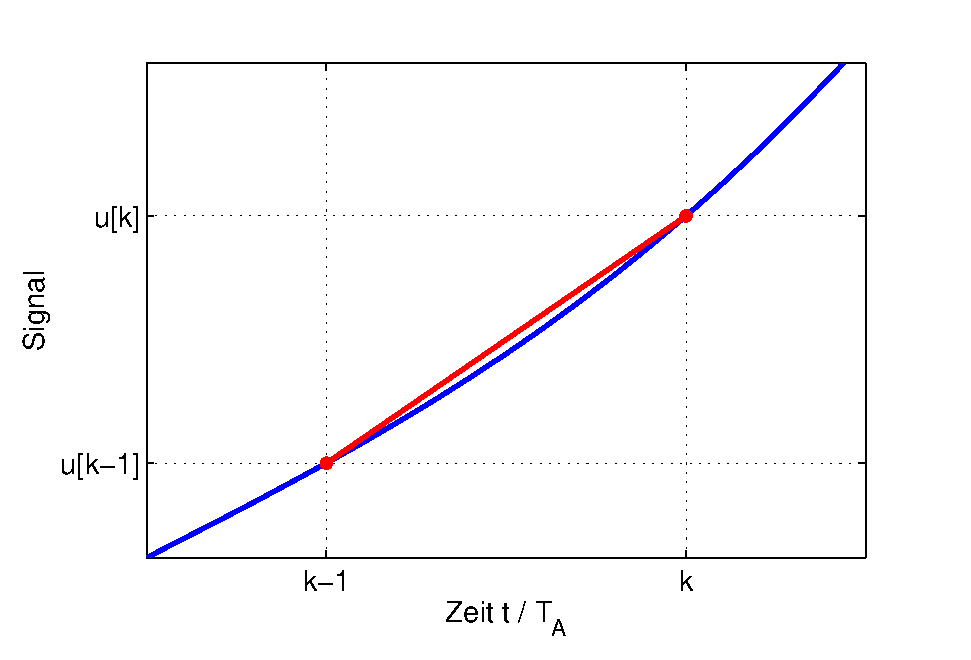
\includegraphics[width=0.5\textwidth]{Kapitel4/Bilder/image4}}
  \caption{Grafische Darstellung der Wahrscheinlichkeitsverteilung aus Gleichung \eqref{eq:fourseventy}}
  \label{fig:SchiefeVerteilung}
\end{figure}

\clearpage

\noindent Durch Einsetzen in die Definitionsgleichungen ergibt sich der Mittelwert zu

\begin{equation}\label{eq:fourseventyone}
\mu =E(x)=\int _{0}^{\infty}{x}^{2} \cdot {e}^{-x}dx=2
\end{equation}

\noindent das zweite Moment zu

\begin{equation}\label{eq:fourseventytwo}
E(x^{2})=\int _{0}^{\infty}{x}^{3} \cdot {e}^{-x} dx =6
\end{equation}

\noindent und das dritte Moment zu

\begin{equation}\label{eq:fourseventythree}
E(x^{3})=\int _{0}^{\infty }{x}^{4} \cdot {e}^{-x} dx =24
\end{equation}

\noindent Mit den Gleichungen \eqref{eq:fourfiftyfive} und \eqref{eq:foursixtyseven} sowie \eqref{eq:fourseventytwo} und \eqref{eq:fourseventythree} k\"{o}nnen die Varianz und die Schiefe der Verteilung berechnet werden zu 

\begin{equation}\label{eq:fourseventyfour}
\sigma ^{2} =E\left((x-\mu)^{2} \right)=E(x^{2})-\mu ^{2} =6-4=2
\end{equation}

\begin{equation}\label{eq:fourseventyfive}
\gamma =\dfrac{1}{\sigma ^{3} } \cdot \left(E(x^{3})-3\cdot \mu \cdot E(x^{2})+2\cdot \mu ^{3} \right)=\dfrac{24-3\cdot 2\cdot 6+2\cdot 8}{2\cdot \sqrt{2} } =\sqrt{2}
\end{equation}

\noindent Es handelt sich um eine Funktion mit positiver Schiefe $\gamma$ = 1.4, die Verteilung ist damit rechtsschief.

\clearpage

{\fontfamily{phv}\selectfont
\noindent\textbf{Lageregeln zur Interpretation der Symmetrie einer Stichprobe}}\smallskip

\noindent Die Symmetrieeigenschaften der Verteilung einer Stichprobe k\"{o}nnen auch an der Lage von Median und Mittelwert abgelesen werden. Auch dazu wird auf die Ausf\"{u}hrungen zur deskriptiven Statistik verwiesen. 

\begin{table}[H]
\setlength{\arrayrulewidth}{.1em}
\caption{Lageregeln von Median und arithmetischem Mittelwert zur Beschreibung der Symmetrie}
\setlength{\fboxsep}{0pt}%
\colorbox{lightgray}{%
\arrayrulecolor{white}%
\begin{tabular}{| c | c |}
\hline
\parbox[c][0.3in][c]{3.3in}{\smallskip\centering\textbf{\fontfamily{phv}\selectfont{Lagekennwerte}}} & 
\parbox[c][0.3in][c]{3.3in}{\smallskip\centering\textbf{\fontfamily{phv}\selectfont{Symmetrieeigenschaft}}}\\ \hline


\parbox[c][0.3in][c]{3.3in}{\centering\fontfamily{phv}\selectfont{$\mu >x_{MED} $}} & 
\parbox[c][0.3in][c]{3.3in}{\centering\fontfamily{phv}\selectfont{Rechtsschiefe Verteilung}} \\
\hline

\parbox[c][0.3in][c]{3.3in}{\centering\fontfamily{phv}\selectfont{$\mu =x_{MED} $}} & 
\parbox[c][0.3in][c]{3.3in}{\centering\fontfamily{phv}\selectfont{Symmetrische Verteilung}} \\
\hline

\parbox[c][0.3in][c]{3.3in}{\centering\fontfamily{phv}\selectfont{$\mu <x_{MED} $}} & 
\parbox[c][0.3in][c]{3.3in}{\centering\fontfamily{phv}\selectfont{Linksschiefe Verteilung}} \\
\hline

\end{tabular}%
}
\label{tab:fourseven}
\end{table}

\clearpage

\subsubsection{Zusammenfassung Kennwerte von Verteilungen}

\noindent Tabelle \ref{tab:foureight} fasst die Kennwerte von Verteilungen zusammen. Die Definition der Parameter \"{u}ber Momente ist von gr\"{o}{\ss}erem praktischen Nutzen und wird in den folgenden Kapiteln weiter ben\"{o}tigt und ausgebaut.

\begin{table}[H]
\setlength{\arrayrulewidth}{.1em}
\caption{Zusammenfassung der Kennwerte von Verteilungen}
\setlength{\fboxsep}{0pt}%
\colorbox{lightgray}{%
\arrayrulecolor{white}%
\begin{tabular}{| wc{5.5cm} | wc{5.5cm} | wc{5.5cm} }
\hline\xrowht{20pt}

\multirow{2}{*}{\fontfamily{phv}\selectfont\textbf{Momente}} & \multicolumn{2}{c}{\fontfamily{phv}\selectfont\textbf{Basis f\"{u}r Definition}} \\ \xrowht{15pt}
& \fontfamily{phv}\selectfont\textbf{Momente} & 
\fontfamily{phv}\selectfont\textbf{Quantile} \\ \hline \xrowht{12.5pt}

\multirow{3}{*}{\fontfamily{phv}\selectfont{Lage}} &
\fontfamily{phv}\selectfont{Mittelwert}  & 
\fontfamily{phv}\selectfont{Median} \\ \xrowht{12.5pt}
& $\mu =E(x^{1})=E(x)$ & $F(x_{MED})=0.5$ \\ \hline\xrowht{12.5pt}

\multirow{3}{*}{\fontfamily{phv}\selectfont{Streuung}} &
\fontfamily{phv}\selectfont{Varianz}  & 
\fontfamily{phv}\selectfont{Inter-Quartil-Range} \\ \xrowht{12.5pt}
& $\sigma ^{2} =E((x-\mu)^{2})$ & $IQR=x_{0.75} -x_{0.25} $ \\ \hline\xrowht{25pt}

\multirow{3}{*}{\fontfamily{phv}\selectfont{Streuung}} &
\fontfamily{phv}\selectfont{Varianz}  & 
\fontfamily{phv}\selectfont{Inter-Quartil-Range} \\ \xrowht{25pt}
& $\gamma =\dfrac{1}{\sigma ^{3} } \cdot E((x-\mu)^{3})$ & $g_{0.25} =\dfrac{(x_{0.75} -x_{0.5})-(x_{0.5} -x_{0.25})}{x_{0.75} -x_{0.25} } $ \\ \hline

\end{tabular}%
}
\label{tab:foureight}
\end{table}

\clearpage

\subsection{Funktionen von Zufallsvariablen}

\noindent Als Zufallsvariable wird allgemein eine Variable bezeichnet, die dem Ergebnis eines Zufallsexperimentes eine reelle Zahl zuordnet. Die reelle Zahl kann \"{u}ber eine Funktion 

\begin{equation}\label{eq:fourseventysix}
y=g(x)
\end{equation}

\noindent abgebildet werden. Es wird von einer Funktion der Zufallsvariable x gesprochen. Bild \ref{fig:DarstellungFunktionVonZufallsvariablen} verdeutlicht die Abbildung der Variable x auf die Variable y \"{u}ber die Funktion g(x).

\noindent 
\begin{figure}[H]
  \centerline{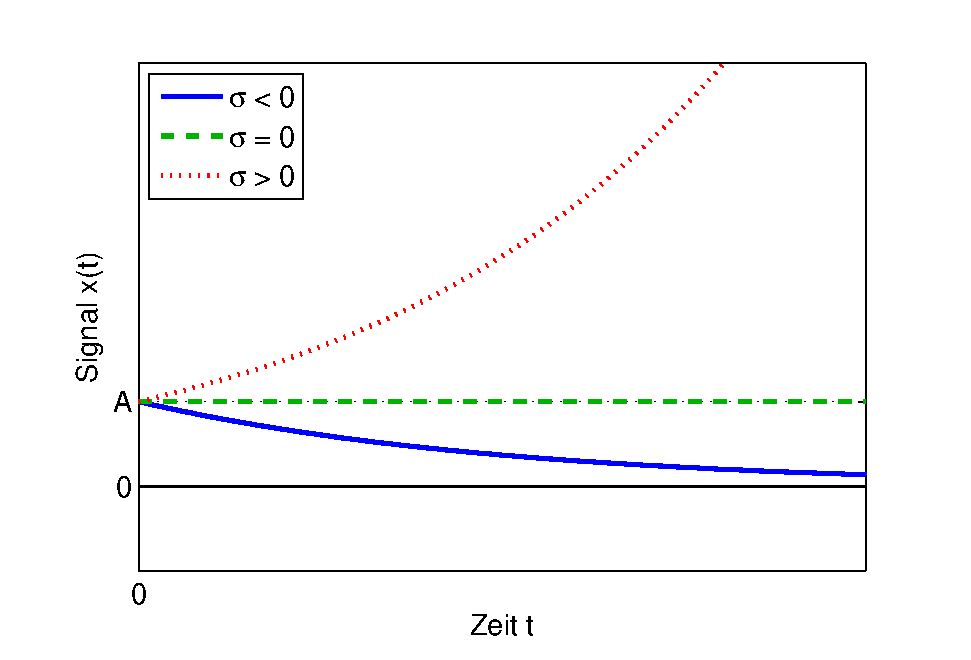
\includegraphics[width=1\textwidth]{Kapitel4/Bilder/image5}}
  \caption{Grafische Veranschaulichung der Funktion von Zufallsvariable}
  \label{fig:DarstellungFunktionVonZufallsvariablen}
\end{figure}

\noindent F\"{u}r die Berechnung praktischer Aufgabenstellungen zur Variable y ist es erforderlich, die Wahrscheinlichkeitsverteilung der Variable y zu kennen. Sie kann berechnet werden, wenn die Verteilungsfunktion der Variable x bekannt ist.

\subsubsection{Funktion einer diskreten Zufallsvariable}

\noindent Bei diskreten Zufallsvariablen wird einem Zufallsereignis eine feste Zahl x$_{n}$ zugeordnet. Durch eine Abbildung

\begin{equation}\label{eq:fourseventyseven}
y_{n} =g(x_{n})
\end{equation}

\noindent ändert sich an der Wahrscheinlichkeit des zugrunde liegenden Ereignisses nichts, sodass sich die Wahrscheinlichkeit von x$_{n}$ auf y$_{n}$ \"{u}bertr\"{a}gt. Bild \ref{fig:DarstellungFunktionVonZufallsvariablen} macht deutlich, dass die Variable y$_{n}$ m\"{o}glicherweise durch unterschiedliche Variable x$_{n}$ erreicht werden kann. Damit errechnet sich die Wahrscheinlichkeit der Zufallsvariable y$_{n}$ \"{a}hnlich wie bei Ereignisb\"{a}umen aus der Summe

\begin{equation}\label{eq:fourseventyeight}
f_{Y} (y_{n})=\sum _{y_{n} =g(x_{n})}f_{X}(x_{n})
\end{equation}

\noindent Bei bekannter Wahrscheinlichkeitsverteilung f$_{Y}$(y) errechnet sich die Verteilungsfunktion der Variable y definitionsgem\"{a}{\ss} zu

\begin{equation}\label{eq:fourseventynine}
F_{Y} (y)=\sum _{y_{n} =-\infty }^{y}f_{Y} (y_{n})
\end{equation}

\clearpage 

\noindent
\colorbox{lightgray}{%
\arrayrulecolor{white}%
\renewcommand\arraystretch{0.6}%
\begin{tabular}{ wl{16.5cm} }
{\fontfamily{phv}\selectfont{Beispiel: Abbildung einer diskreten Zufallsvariable}}
\end{tabular}%
}\medskip 

\noindent Gegeben ist eine Zufallsvariable x. Ihr Ereignisraum und ihre Wahrscheinlichkeitsverteilung sind in Tabelle \ref{tab:fournine} dargestellt. Die Zufallsvariable x wird \"{u}ber die Funktion 

\begin{equation}\label{eq:foureighty}
y=(x-1)^{2}
\end{equation}

\noindent auf eine Zufallsvariable y abgebildet. Sie ist ebenfalls in Tabelle \ref{tab:fournine} aufgef\"{u}hrt.

\begin{table}[H]
\caption{Diskrete Zufallsvariable x und ihre Wahrscheinlichkeitsverteilung $f_{X}(x)$}
\setlength{\fboxsep}{0pt}%
\colorbox{lightgray}{%
\arrayrulecolor{white}%
\begin{tabular}{| c | c | c | c | c | c |}
\hline

\parbox[c][0.28in][c]{0.97in}{\smallskip\centering\textbf{\fontfamily{phv}\selectfont{$x_{n}$}}} &
\parbox[c][0.28in][c]{0.97in}{\centering{-1}} &
\parbox[c][0.28in][c]{0.97in}{\centering{0}} &
\parbox[c][0.28in][c]{0.97in}{\centering{1}} &
\parbox[c][0.28in][c]{0.97in}{\centering{2}} &
\parbox[c][0.28in][c]{0.97in}{\centering{3}} \\ \hline

\parbox[c][0.28in][c]{0.97in}{\smallskip\centering\textbf{\fontfamily{phv}\selectfont{$f_{X}(x_{n})$}}} &
\parbox[c][0.28in][c]{0.97in}{\centering{0.1}} &
\parbox[c][0.28in][c]{0.97in}{\centering{0.2}} &
\parbox[c][0.28in][c]{0.97in}{\centering{0.4}} &
\parbox[c][0.28in][c]{0.97in}{\centering{0.2}} &
\parbox[c][0.28in][c]{0.97in}{\centering{0.1}} \\ \hline

\parbox[c][0.28in][c]{0.97in}{\smallskip\centering\textbf{\fontfamily{phv}\selectfont{$y_{n}$}}} &
\parbox[c][0.28in][c]{0.97in}{\centering{4}} &
\parbox[c][0.28in][c]{0.97in}{\centering{1}} &
\parbox[c][0.28in][c]{0.97in}{\centering{0}} &
\parbox[c][0.28in][c]{0.97in}{\centering{1}} &
\parbox[c][0.28in][c]{0.97in}{\centering{4}} \\ \hline

\end{tabular}%
}\bigskip
\label{tab:fournine}
\end{table}

\noindent Da zum Beispiel der Wert y = 1 \"{u}ber x = 0 und x = 2 erreicht werden kann, werden die entsprechenden Wahrscheinlichkeiten f\"{u}r das Ereignis y = 1 addiert.

\begin{equation}\label{eq:foureightyone}
f_{Y} (y=1)=f_{X}(x=0)+f_{X} (x=2)=0.2+0.2=0.4
\end{equation}

\noindent Es ergibt sich die in Tabelle \ref{tab:fourten} gezeigte Wahrscheinlichkeitsverteilung und Verteilungsfunktion der Zufallsvariable y.

\begin{table}[H]
\caption{Diskrete Zufallsvariable y und ihre Wahrscheinlichkeitsverteilung $f_{Y}(y)$}
\setlength{\fboxsep}{0pt}%
\colorbox{lightgray}{%
\arrayrulecolor{white}%
\begin{tabular}{| c | c | c | c |}
\hline

\parbox[c][0.28in][c]{1.54in}{\smallskip\centering\textbf{\fontfamily{phv}\selectfont{$y_{n}$}}} &
\parbox[c][0.28in][c]{1.54in}{\centering{0}} &
\parbox[c][0.28in][c]{1.54in}{\centering{1}} &
\parbox[c][0.28in][c]{1.54in}{\centering{4}} \\ \hline

\parbox[c][0.28in][c]{1.54in}{\smallskip\centering\textbf{\fontfamily{phv}\selectfont{$f_{Y}(y_{n})$}}} &
\parbox[c][0.28in][c]{1.54in}{\centering{0.4}} &
\parbox[c][0.28in][c]{1.54in}{\centering{0.4}} &
\parbox[c][0.28in][c]{1.54in}{\centering{0.2}}  \\ \hline

\parbox[c][0.28in][c]{1.54in}{\smallskip\centering\textbf{\fontfamily{phv}\selectfont{$F_{Y}(y_{n})$}}} &
\parbox[c][0.28in][c]{1.54in}{\centering{0.4}} &
\parbox[c][0.28in][c]{1.54in}{\centering{0.8}} &
\parbox[c][0.28in][c]{1.54in}{\centering{1}}  \\ \hline

\end{tabular}%
}\bigskip
\label{tab:fourten}
\end{table}

\subsubsection{Funktion einer kontinuierlichen Zufallsvariable}

\noindent Auch bei kontinuierlichen Zufallsvariablen wird einem Zufallsereignis eine Zahl x zugeordnet. Durch die Abbildung

\begin{equation}\label{eq:foureightytwo}
y=g(x)
\end{equation}

\noindent entsteht eine Zufallsvariable y, deren Verteilungsfunktion F$_{Y}$(y) im Folgenden f\"{u}r streng monoton steigende Funktionen g(x) hergeleitet wird. Die Verteilungsfunktion F$_{Y}$(y) ist definiert als die Wahrscheinlichkeit, dass eine Variable $\psi$ kleiner als der Wert y ist. Da die Zufallsvariable $\psi$ = g($\xi$) definiert ist, gilt

\begin{equation}\label{eq:foureightythree}
yF_{Y} (y)=P\left(\psi \le y\right)=P\left(g(\xi)\le y\right)
\end{equation}

\clearpage

\noindent Die Funktion g(x) ist streng monoton steigend. Damit gilt:

\begin{equation}\label{eq:foureightyfour}
F_{Y} (y)=P\left(\xi \le g^{-1} (y)\right)=F_{X} (g^{-1}(y))
\end{equation}

\noindent Aus der Verteilungsfunktion F$_{Y}$(y) errechnet sich die Wahrscheinlichkeitsdichte f$_{Y}$(y) mit der Kettenregel der Differentiationsrechnung zu

\begin{equation}\label{eq:foureightyfive}
f_{Y} (y)=\dfrac{dF_{Y}}{dy} =\dfrac{dF_{X} (g^{-1} (y))}{dg^{-1} (y)} \cdot \dfrac{dg^{-1} (y)}{dy} =f_{X} (g^{-1} (y))\cdot \dfrac{dg^{-1} (y)}{dy}
\end{equation}

\noindent Die Regel kann auf Funktionen g(x) verallgemeinert werden, die streng monoton sind. Es ergibt sich

\begin{equation}\label{eq:foureightysix}
f_{Y} (y)=\dfrac{dF_{Y} }{dy} =\dfrac{dF_{X} \left(g^{-1} (y)\right)}{dg^{-1} (y)} \cdot \dfrac{dg^{-1} \left(y\right)}{dy} =f_{X} (g^{-1} (y))\cdot \left|\dfrac{dg^{-1} (y)}{dy} \right|
\end{equation}

\noindent
\colorbox{lightgray}{%
\arrayrulecolor{white}%
\renewcommand\arraystretch{0.6}%
\begin{tabular}{ wl{16.5cm} }
{\fontfamily{phv}\selectfont{Beispiel: Abbildung einer kontinuierlichen Zufallsvariable}}
\end{tabular}%
}\medskip 

\noindent Gegeben ist eine Zufallsvariable x, die in dem Bereich 0 $\mathrm{<}$ x $\leq$ 2 eine Wahrscheinlichkeitsdichte 

\begin{equation}\label{eq:foureightyseven}
f_{X} (x)=\dfrac{1}{2} \cdot x
\end{equation}

\noindent und Verteilungsfunktion

\begin{equation}\label{eq:foureightyeight}
F_{X} \left(x\right)=\dfrac{1}{4} \cdot x^{2}
\end{equation}

\noindent aufweist. Beide Funktionen sind in Bild \ref{fig:FunktionVonZufallsvariablen1} dargestellt.

\noindent 
\begin{figure}[H]
  \centerline{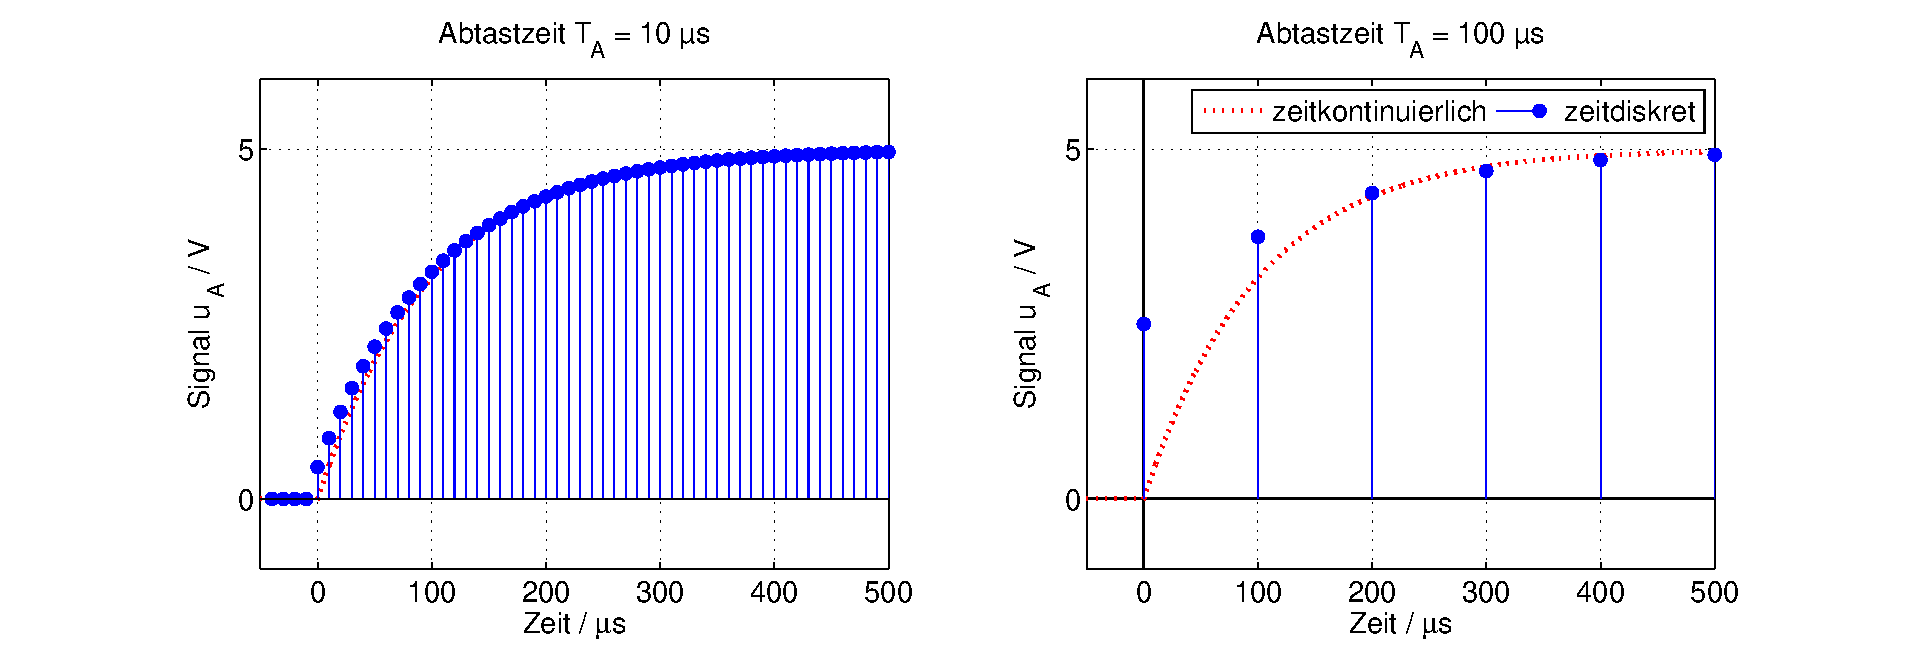
\includegraphics[width=1\textwidth]{Kapitel4/Bilder/image6}}
  \caption{Wahrscheinlichkeitsdichte f$_{X}$(x) und Verteilungsfunktion F$_{X}$(x) der kontinuierlichen Zufallsvariable x}
  \label{fig:FunktionVonZufallsvariablen1}
\end{figure}

\clearpage

\noindent Die Zufallsvariable x wird mit der Funktion 

\begin{equation}\label{eq:foureightynine}
y=g(x)=\dfrac{1}{2} \cdot x^{2}
\end{equation}

\noindent auf die Zufallsvariable y abgebildet. In dem Bereich von 0 $\mathrm{<}$ x $\leq$ 2 lautet die Umkehrfunktion

\begin{equation}\label{eq:fourninety}
x=g^{-1} (y)=\sqrt{2\cdot y}
\end{equation}

\noindent Die Verteilungsfunktion der Variable y errechnet sich zu

\begin{equation}\label{eq:fourninetyone}
F_{Y} (y)=F_{X} \left(g^{-1} (y)\right)=\left. \dfrac{1}{4} \cdot x^{2} \right|_{x=\sqrt{2\cdot y}} =\dfrac{1}{4} \cdot 2\cdot y=\dfrac{1}{2} \cdot y
\end{equation}

\noindent In dem relevanten Bereich von 0 $\mathrm{<}$ x $\leq$ 2 ist die Funktion g(x) streng monoton steigend. Damit ergibt sich die Wahrscheinlichkeitsdichte

\begin{equation}\label{eq:fourninetytwo}
f_{Y} (y)=f_{X} \left(g^{-1} (y)\right)\cdot \left|\dfrac{dg^{-1} (y)}{dy} \right|=\left. \dfrac{1}{2} \cdot x\right|_{x=\sqrt{2\cdot u}} \cdot \dfrac{d}{du} \sqrt{2\cdot u} =\dfrac{1}{2} \cdot \sqrt{2\cdot u} \cdot \sqrt{2} \cdot \dfrac{1}{2} \cdot \dfrac{1}{\sqrt{u}} =\dfrac{1}{2}
\end{equation}

\noindent Wahrscheinlichkeitsdichte und Verteilungsfunktion der Zufallsvariable y sind in Bild \ref{fig:FunktionVonZufallsvariablen2} dargestellt.

\noindent 
\begin{figure}[H]
  \centerline{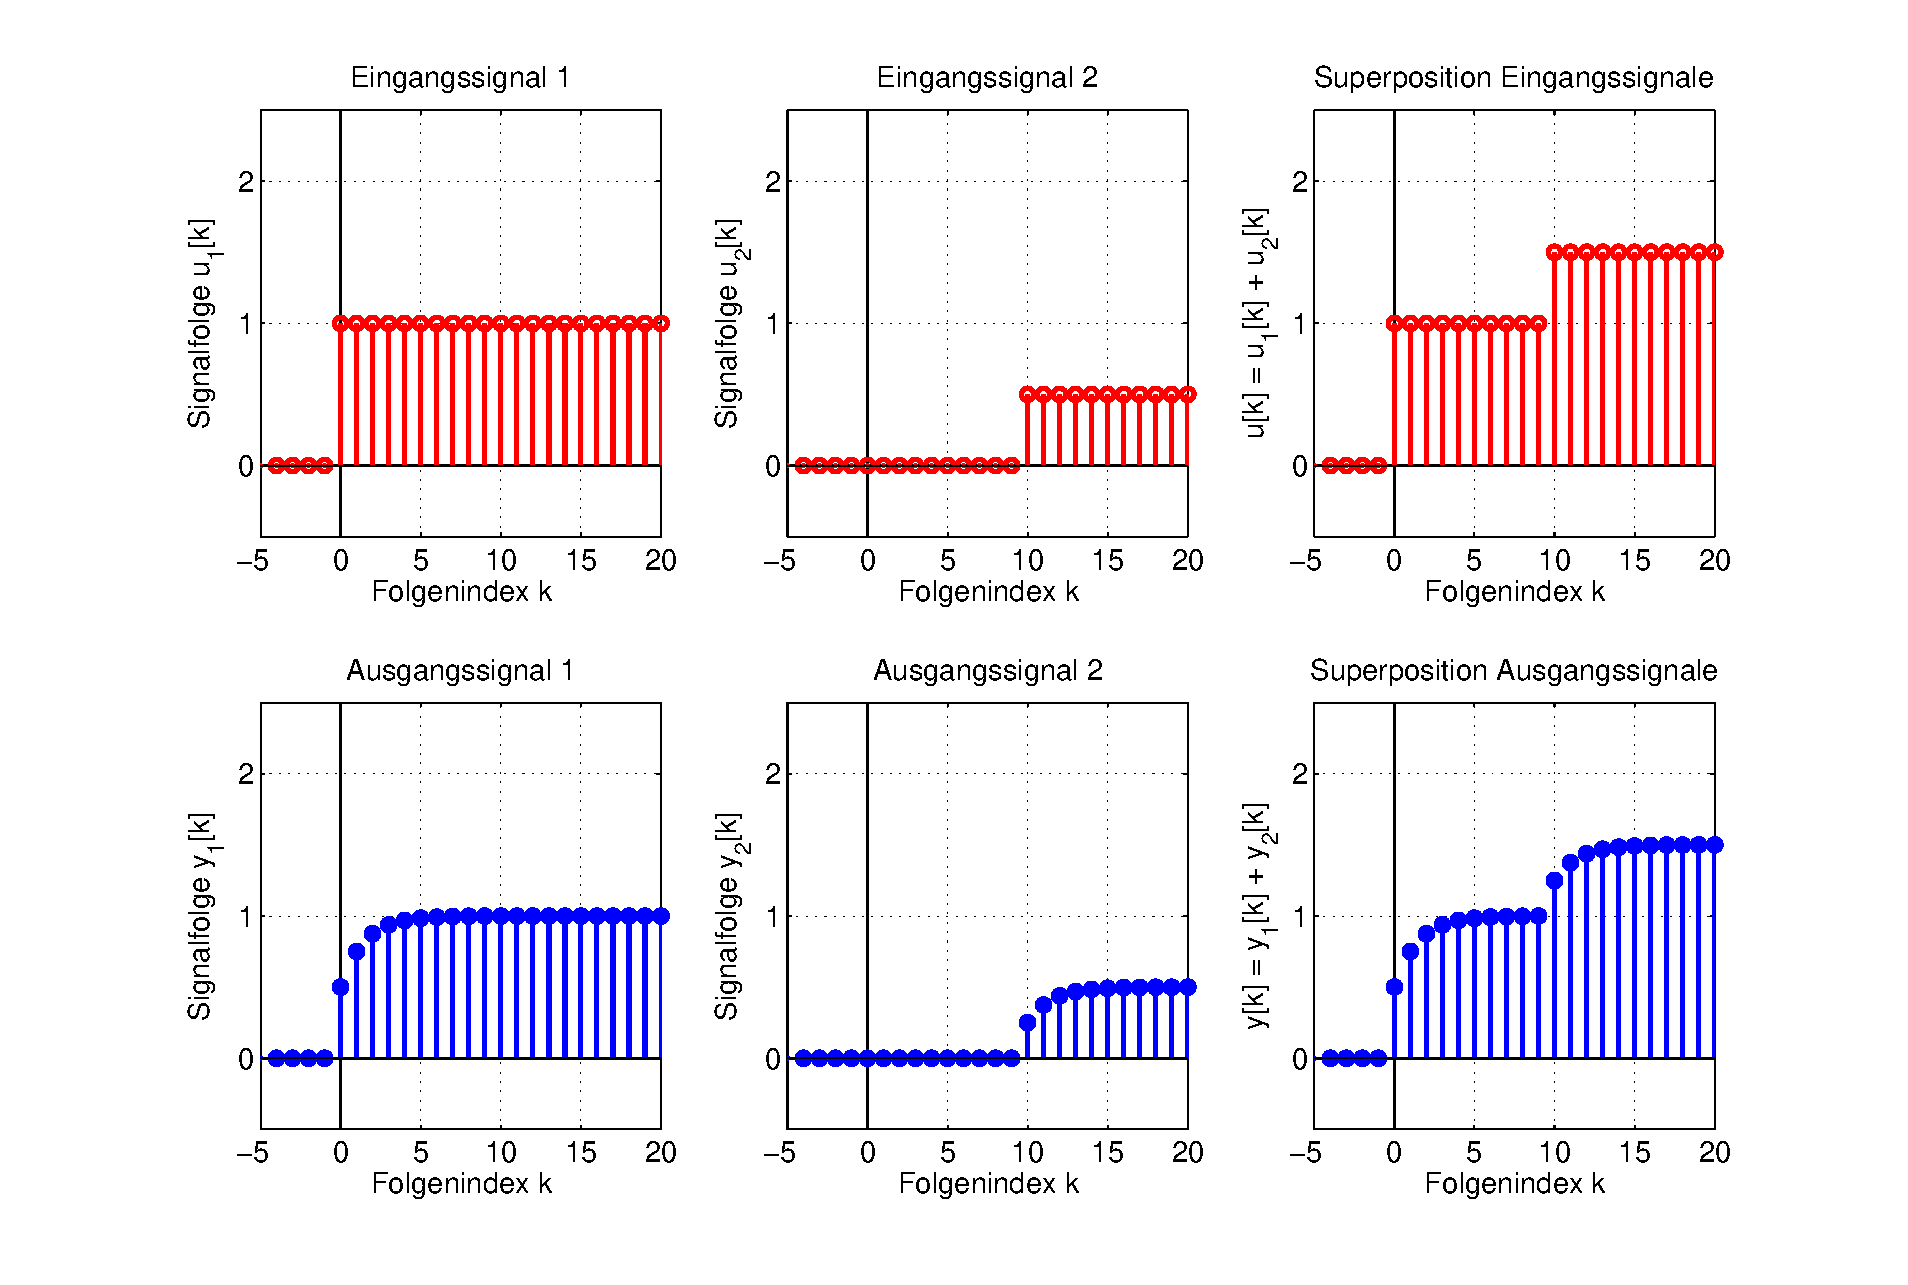
\includegraphics[width=1\textwidth]{Kapitel4/Bilder/image7}}
  \caption{Wahrscheinlichkeitsdichte f$_{Y}$(y) und Verteilungsfunktion F$_{Y}$(y) der kontinuierlichen Zufallsvariable y}
  \label{fig:FunktionVonZufallsvariablen2}
\end{figure}

\noindent Die Abbildung von Zufallsvariablen hat zwei wichtige Anwendungen: die Standardisierung von Zufallsvariablen und die numerische Generierung von Zufallsvariablen mit einer definierten Verteilung.


\subsubsection{Lineare Abbildung und Standardisierung einer Zufallsvariable}\label{fourthree}

\noindent Eine Zufallsvariable y ist über die lineare Abbildung 

\begin{equation}\label{eq:fourninetythree}
y=a\cdot x+b
\end{equation}

\noindent mit a $\mathrm{>}$ 0 definiert. Ihre Wahrscheinlichkeitsdichte errechnet sich nach Gleichung \eqref{eq:foureightysix} zu

\begin{equation}\label{eq:fourninetyfour}
f_{Y} (y)=f_{X} \left(\dfrac{y-b}{a} \right)\cdot \left|\dfrac{1}{a} \right|
\end{equation}

\noindent Die Zufallsvariable y besitzt einen Mittelwert von

\begin{equation}\label{eq:fourninetyfive}
\mu _{y} =E(y)=E\left(a\cdot x+b\right)=a\cdot E(x)+b=a\cdot \mu _{x} +b
\end{equation}

\noindent und eine Varianz von

\begin{equation}\label{eq:fourninetysix}
\begin{split}
\sigma _{y}^{2} & = E\left((y-\mu _{y})^{2} \right)=E\left(y^{2} \right)-E(y)^{2} =E\left((a\cdot x+b)^{2} \right)-E(a\cdot x+b)^{2}\\
& = E\left( a^{2}\cdot x^{2} + 2\cdot a\cdot b\cdot x + b^{2} \right) - \left(E(a\cdot x)^{2} + 2\cdot E(a\cdot x)\cdot E(b)+E(b)^{2} \right )\\
& = a^{2}\cdot E\left(x^{2}\right )+2\cdot a \cdot b\cdot E(x)+b^{2}-a^{2}\cdot E(x)^{2}-2\cdot a\cdot b\cdot E(x) -b^{2}\\
& = a^{2}\cdot \left(E(x^{2})-E(x)^{2}\right ) = a^{2} \cdot \sigma _{x}^{2}
\end{split}
\end{equation}

\noindent Die Standardabweichung der Zufallsvariablen y ergibt sich aus der positiven Wurzel der Varianz zu

\begin{equation}\label{eq:fourninetyseven}
\sigma _{y} =\sqrt{\sigma _{y}^{2}} =\sqrt{a^{2} \cdot \sigma _{x}^{2}} =a\cdot \sigma _{x}
\end{equation}

\noindent Ein Sonderfall der linearen Abbildung ist die Standardisierung von Zufallsvariablen. Standardisierte Zufallsvariablen weisen einen Mittelwert von $\mu_{y}$ = 0 und eine Standardabweichung von $\sigma_{y}$ = 1 auf. Aus diesen beiden Bedingungen ergeben sich zwei Gleichungen f\"{u}r die beiden unbekannten Variablen a und b:

\begin{equation}\label{eq:fourninetyeight}
\mu _{y} =a\cdot \mu _{x} +b=0
\end{equation}

\begin{equation}\label{eq:fourninetynine}
\sigma _{y}^{2} =a^{2} \cdot \sigma _{x}^{2} =1
\end{equation}

\noindent Aus den Bedingungen f\"{u}r a und b 

\begin{equation}\label{eq:fourhundred}
a=\dfrac{1}{\sigma _{x}}
\end{equation}

\noindent und 

\begin{equation}\label{eq:fourhundredone}
b=-\dfrac{\mu _{x} }{\sigma _{x}}
\end{equation}

\noindent ergibt sich die standardisierte Zufallsvariable

\begin{equation}\label{eq:fourhundredtwo}
y=a\cdot x+b=\dfrac{x}{\sigma _{x} } -\dfrac{\mu _{x}}{\sigma _{x}} =\dfrac{x-\mu _{x}}{\sigma _{x}}
\end{equation}

\noindent Standardisierte Zufallsvariablen sind mittelwertfrei und weisen eine Varianz von 1 auf. Sie sind insbesondere im Zusammenhang von Testverteilungen von Bedeutung.\bigskip

\noindent
\colorbox{lightgray}{%
\arrayrulecolor{white}%
\renewcommand\arraystretch{0.6}%
\begin{tabular}{ wl{16.5cm} }
{\fontfamily{phv}\selectfont{Beispiel: Gl\"{u}cksrad}}
\end{tabular}%
}\medskip 

\noindent Die Standardisierung von Zufallsvariablen wird an dem Beispiel des Gl\"{u}cksrads vertieft. Mit dem Mittelwert 

\begin{equation}\label{eq:fourhundredthree}
\mu _{x} =\pi 
\end{equation}

\noindent und der Standardabweichung von 

\begin{equation}\label{eq:fourhundredfour}
\sigma _{x} =\dfrac{1}{\sqrt{3}} \cdot \pi
\end{equation}

\noindent ergibt sich die Abbildungsgleichung zu

\begin{equation}\label{eq:fourhundredfive}
y=\dfrac{x-\mu _{x}}{\sigma _{x}} =\dfrac{x-\pi}{\dfrac{1}{\sqrt{3}} \cdot \pi } =\sqrt{3} \cdot \dfrac{x-\pi}{\pi}
\end{equation}

\noindent Durch die Transformation werden die Intervallgrenzen von 0 und 2$\pi$ abgebildet auf

\begin{equation}\label{eq:fourhundredsix}
y_{\min } =\sqrt{3} \cdot \dfrac{0-\pi}{\pi} =-\sqrt{3}
\end{equation}

\noindent und 

\begin{equation}\label{eq:fourhundredseven}
y_{\max} =\sqrt{3} \cdot \dfrac{2\cdot \pi -\pi}{\pi} =\sqrt{3}
\end{equation}

\noindent Die Wahrscheinlichkeitsdichte ergibt sich in dem Zahlenbereich y$_{min}$ $\mathrm{<}$ y $\leq$ y$_{max}$ aus der Bedingung f\"{u}r das sichere Ereignis zu

\begin{equation}\label{eq:fourhundredeight}
f(y)=\dfrac{1}{2\cdot \sqrt{3}}
\end{equation}

Bild \ref{fig:Standardisierung} stellt f\"{u}r das Gl\"{u}cksrad die Verteilung der Zufallsvariable x und der standardisierten Zufallsvariable y gegen\"{u}ber.

\noindent 
\begin{figure}[H]
  \centerline{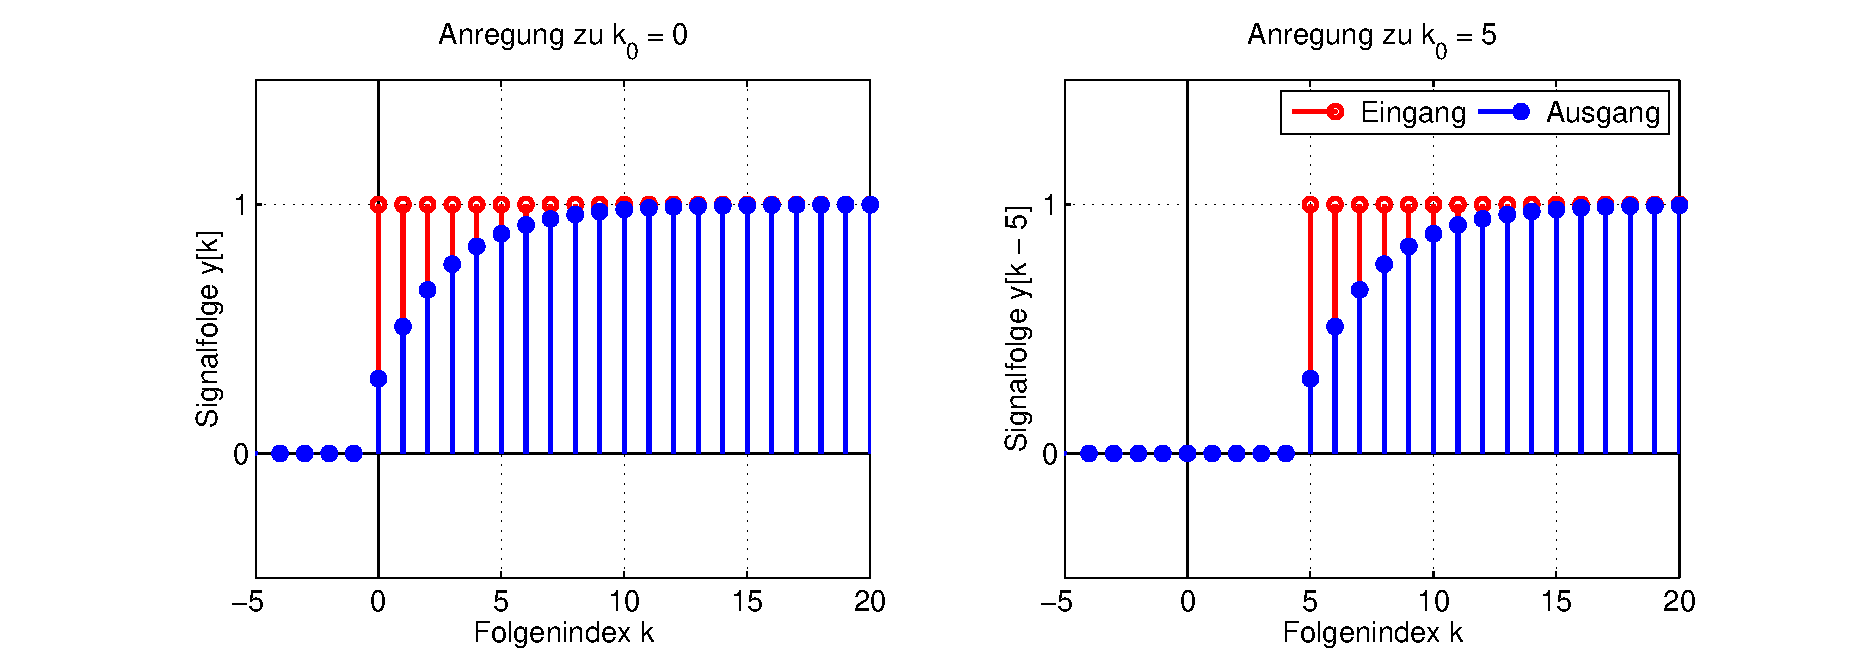
\includegraphics[width=1\textwidth]{Kapitel4/Bilder/image8}}
  \caption{Grafische Darstellung der Wahrscheinlichkeitsverteilung f\"{u}r das Beispiel Gl\"{u}cksrad mit und ohne Standardisierung}
  \label{fig:Standardisierung}
\end{figure}

\noindent Nach der Standardisierung der Zufallsvariable ist die Verteilung symmetrisch um den Mittelwert $\mu_{y}$ = 0. Die Varianz ergibt sich erwartungsgem\"{a}{\ss} zu

\begin{equation}\label{eq:fourhundrednine}
\sigma _{y}^{2} =\int _{-\infty}^{\infty}(y-\mu _{y})^{2} \cdot {f}\left(y\right){dy} =\int _{-\sqrt{3}}^{\sqrt{3}}y^{2} \cdot \dfrac{1}{2\cdot \sqrt{3}} {dy} =\dfrac{{\rm 1}}{2\cdot \sqrt{3}} \cdot \dfrac{1}{3} \cdot \left(3\cdot \sqrt{3} +3\cdot \sqrt{3} \right)=1
\end{equation}

\subsubsection{Generierung von Zufallszahlen mit einer definierten Verteilung}

\noindent In Programmen werden zur Generierung von Zufallszahlen Generatoren eingesetzt, die quasizuf\"{a}llig einen Wert 0 $\mathrm{<}$ x $\leq$ 1 erzeugen. Die Wahrscheinlichkeitsdichte dieser Zahlen ist typischerweise gleichverteilt.

\begin{equation}\label{eq:fourhundredten}
f_{X} (x)=1
\end{equation}

\noindent Die Zufallsvariable besitzt damit im Zahlenbereich 0 $\mathrm{<}$ x $\leq$ 1 die Verteilungsfunktion

\begin{equation}\label{eq:fourhundredeleven}
F_{X} (x)=x
\end{equation}

\noindent Um Zufallszahlen y mit einer beliebigen Verteilung F${}_{Y}$(y) zu generieren, wird die Funktion

\begin{equation}\label{eq:fourhundredtwelve}
y=F_{Y}^{-1} (x)
\end{equation}

\noindent berechnet. Nach Gleichung \eqref{eq:foureightysix} besitzt sie die Wahrscheinlichkeitsdichte

\begin{equation}\label{eq:fourhundredthirteen}
f_{X} \left(g^{-1} (y)\right)\cdot \left|\dfrac{dg^{-1} \left(y\right)}{dy} \right|=1\cdot \left|\dfrac{dF(y)}{dy} \right|=f_{Y} (y)
\end{equation}

\clearpage

\subsection{Spezielle diskrete Verteilungen}

\noindent Viele diskrete Fragestellungen der Wahrscheinlichkeitsrechnung lassen sich mit wenigen speziellen, diskreten Verteilungen beschreiben. Sie ergeben sich aus der Wahrscheinlichkeitstheorie und werden im Folgenden beschrieben.

\subsubsection{Diskrete Gleichverteilung}

\noindent Weisen bei einem Zufallsexperiment alle m\"{o}glichen Werte x$_{n}$ der Zufallsvariable x die gleiche Wahrscheinlichkeit p auf, ergibt sich aus der Bedingung f\"{u}r das sichere Ereignis

\begin{equation}\label{eq:fourhundredfourteen}
1=\sum _{n=1}^{N}f(x_{n}) =\sum _{n=1}^{N}p =N\cdot p
\end{equation}

\noindent Damit lautet die Wahrscheinlichkeitsverteilung 

\begin{equation}\label{eq:fourhundredfifteen}
f(x)=p=\dfrac{1}{N}
\end{equation}

\noindent und die Verteilungsfunktion berechnet sich zu

\begin{equation}\label{eq:fourhundredsixteen}
F(x)=\sum _{x_{n} =0}^{x}p =\sum _{x_{n} =0}^{x}\dfrac{1}{N}
\end{equation}

\noindent Zum Beispiel sind bei einem W\"{u}rfelexperiment mit einem regelm\"{a}{\ss}igen W\"{u}rfel die Wahrscheinlichkeiten f\"{u}r eine beliebige Augenzahl mit 

\begin{equation}\label{eq:fourhundredseventeen}
p=\dfrac{1}{6}
\end{equation}

\noindent gleichverteilt. Die Wahrscheinlichkeitsverteilung und Verteilungsfunktion der Gleichverteilung sind in Bild \ref{fig:Diskret_Gleichverteilung} dargestellt. Die Wahrscheinlichkeitsverteilung f(x) ist konstant, die Verteilungsfunktion F(x) nimmt an jeder Stelle, an der ein m\"{o}glicher Wert der Zufallsvariable steht, zu. 

\noindent 
\begin{figure}[H]
  \centerline{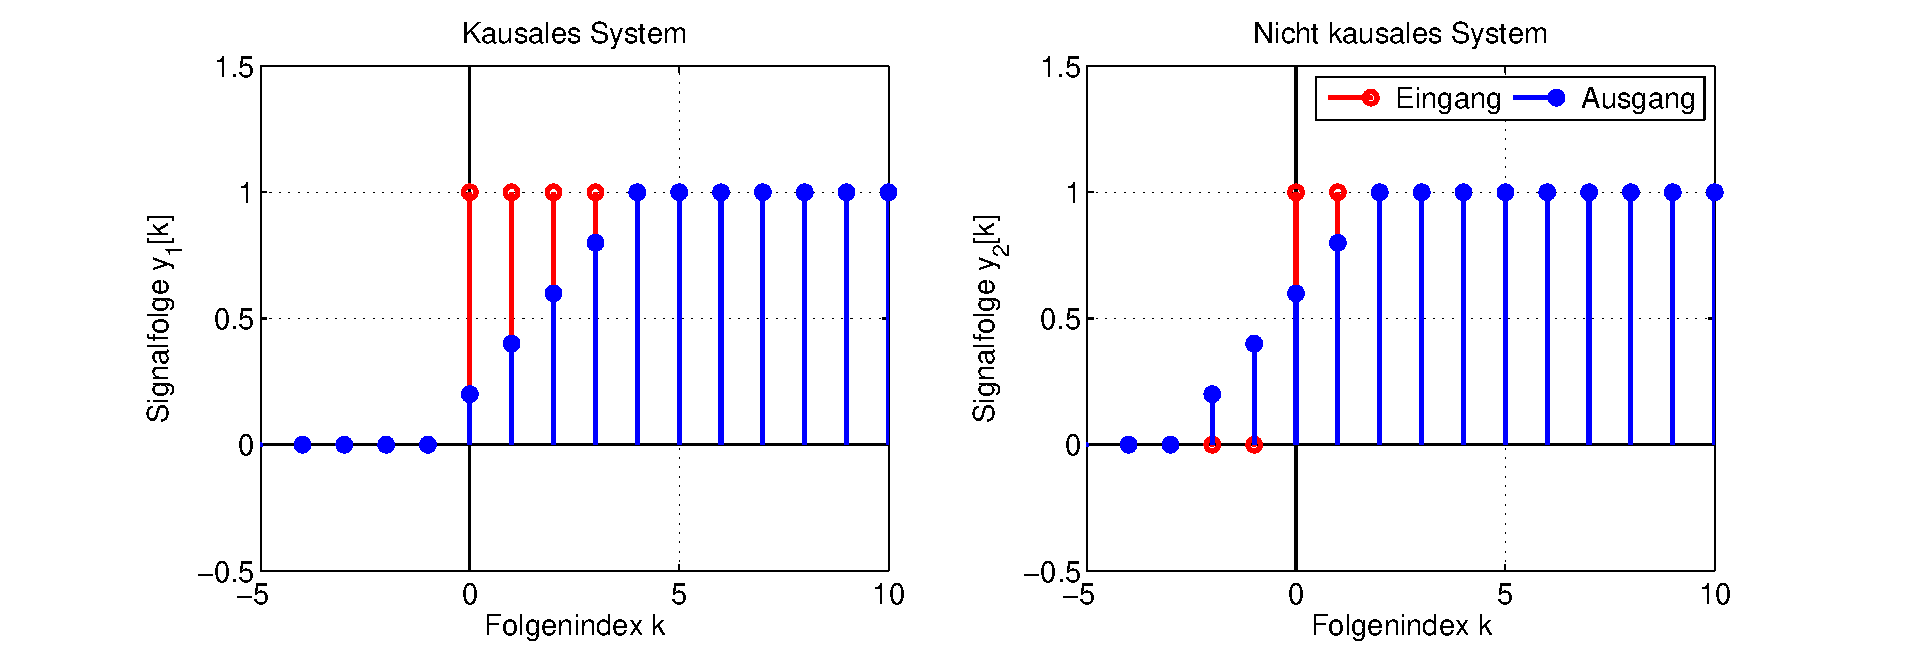
\includegraphics[width=1\textwidth]{Kapitel4/Bilder/image9}}
  \caption{Grafische Darstellung der Wahrscheinlichkeitsverteilung f(x) und Verteilungsfunktion F(x) f\"{u}r das W\"{u}rfeln einer Augenzahl x}
  \label{fig:Diskret_Gleichverteilung}
\end{figure}

\clearpage

\noindent Der Mittelwert der Gleichverteilung errechnet sich aus 

\begin{equation}\label{eq:fourhundredeighteen}
\mu =E(x)=\dfrac{1}{N} \cdot \sum _{n=1}^{N}x_{n}
\end{equation}

\noindent und die Varianz ergibt sich zu

\begin{equation}\label{eq:fourhundrednineteen}
\sigma ^{2} =E\left((x-\mu )^{2} \right)=\dfrac{1}{N} \cdot \sum _{n=1}^{N}(x_{n} -\mu)^{2} 
\end{equation}

\noindent
\colorbox{lightgray}{%
\arrayrulecolor{white}%
\renewcommand\arraystretch{0.6}%
\begin{tabular}{ wl{16.5cm} }
{\fontfamily{phv}\selectfont{Beispiel: Bewertung zweier Anlagem\"{o}glichkeiten}}
\end{tabular}%
}\medskip 

\noindent Dem Kunden einer Bank werden zur Geldanlage zwei m\"{o}gliche Anlagestrategien angeboten. Als konventionelle Variante steht eine Festgeldanlage mit einer festen Verzinsung von j\"{a}hrlich 3.33 \% zur Verf\"{u}gung. Als weitere Anlagevariante wird dem Kunden ein Modell auf Basis von Wertpapieren angeboten. Dabei wird in Abh\"{a}ngigkeit eines Wirtschaftsindex ein Zinssatz von 1.5, 2.5 oder 5 \% ausgezahlt. Da \"{u}ber den Verlauf des Wirtschaftsindex f\"{u}r das Anlagejahr keine Vorhersagen getroffen werden k\"{o}nnen, haben alle drei m\"{o}glichen Zinsbetr\"{a}ge eine gleich hohe Wahrscheinlichkeit, sie sind somit gleichverteilt. Bild \ref{fig:Diskret_Gleichverteilung_Anlagemoeglichkeiten} zeigt die resultierende Wahrscheinlichkeitsverteilung f(x) und die Verteilungsfunktion F(x).

\noindent 
\begin{figure}[H]
  \centerline{\includegraphics[width=1\textwidth]{Kapitel4/Bilder/image10}}
  \caption{Grafische Darstellung der Wahrscheinlichkeitsverteilung f(x) und Verteilungsfunktion F(x) f\"{u}r die Verzinsung bei Wertpapieren}
  \label{fig:Diskret_Gleichverteilung_Anlagemoeglichkeiten}
\end{figure}

\noindent Um zu entscheiden, bei welcher Anlagevariante mit h\"{o}heren Zinsertr\"{a}gen gerechnet werden kann, wird der Erwartungswert beziehungsweise der Mittelwert der zweiten Anlagevariante bestimmt. Dieser folgt zu

\begin{equation}\label{eq:fourhundredtwenty}
\mu =\dfrac{1}{N} \cdot \sum _{n=1}^{N}x_{n} =\dfrac{1}{3} \cdot (1.5+2.5+5)=3 \%
\end{equation}

\noindent Im Mittel wird der Kunde bei der Anlagevariante auf Basis des Wirtschaftsindex eine j\"{a}hrliche Verzinsung von 3 \% erhalten. Da die mittlere Zinserwartung bei h\"{o}herem Risiko geringer ist als bei der Festgeld-Anlage, ist die Festgeld-Anlage zu bevorzugen. 

\clearpage 

\noindent Die Erstellung von Bild \ref{fig:Diskret_Gleichverteilung_Anlagemoeglichkeiten} und die Berechnung des Mittelwertes wurde mit MATLAB durchgef\"{u}hrt.

\lstinputlisting[caption = {}]{Kapitel4/mat1.m}

\noindent Alternativ kann die Umsetzung in Python erfolgen.

\lstinputlisting[caption = {}]{Kapitel4/mat2.m}

\clearpage 

\subsubsection{Bernoulli-Verteilung}

\noindent Ein Spezialfall diskreter Verteilungen ist die Bernoulli-Verteilung, die ein Bernoulli Experiment beschreibt. Dabei wird gepr\"{u}ft, ob ein Ereignis bei einfacher Ausf\"{u}hrung des Experimentes eingetreten ist oder nicht. Die Zufallsvariable x ist damit definiert \"{u}ber

\begin{equation}\label{eq:fourhundredtwentyone}
x=\left\{\begin{array}{l} {1 \qquad \text{für das günstige Ereignis A}} \\ 
{0\qquad \text{für das ungünstige Ereignis A'}} \end{array}\right.
\end{equation}

\noindent Eine solche Variable wird als bin\"{a}re oder Bernoulli-Variable bezeichnet. Ist die Wahrscheinlichkeit f\"{u}r das g\"{u}nstige Ereignis A

\begin{equation}\label{eq:fourhundredtwentytwo}
P(A)=f(1)=p
\end{equation}

\noindent errechnet sich die Wahrscheinlichkeit f\"{u}r das ung\"{u}nstige Ereignis A' zu

\begin{equation}\label{eq:fourhundredtwentythree}
P(A')=f(0)=1-p=q
\end{equation}

\noindent Die Wahrscheinlichkeitsverteilung hat nur die beiden Werte p und q = 1 - p. Der Mittelwert der Bernoulli-Verteilung errechnet sich zu

\begin{equation}\label{eq:fourhundredtwentyfour}
\mu =E(x)=\sum _{n=1}^{2}x_{n} \cdot P(x_{n}) =0\cdot q+1\cdot p=p
\end{equation}

\noindent und die Varianz betr\"{a}gt 

\begin{equation}\label{eq:fourhundredtwentyfive}
\sigma ^{2} =E\left((x-\mu)^{2} \right)=E\left(x^{2} \right)-\mu ^{2} =p-p^{2} =p\cdot q
\end{equation}

\noindent Beispiele f\"{u}r Bernoulli-Experimente sind die Funktion von Bauelementen oder das Erf\"{u}llen von Spezifikationsmerkmalen. Bernoulli-Variablen erlauben jedoch nur eine grobe Kategorisierung von Ereignissen, eine feine Einteilung zum Beispiel nach der Frage, wie weit ein Grenzwert \"{u}berschritten wurde, k\"{o}nnen mit dem Bernoulli-Experiment nicht beantwortet werden.

\noindent
\colorbox{lightgray}{%
\arrayrulecolor{white}%
\renewcommand\arraystretch{0.6}%
\begin{tabular}{ wl{16.5cm} }
{\fontfamily{phv}\selectfont{Beispiel: Bit-Fehler bei der digitalen Signal\"{u}bertragung}}
\end{tabular}%
}\medskip 

\noindent Als Anwendungsbeispiel f\"{u}r die Bernoulli-Verteilung wird die \"{U}bertragung eines stochastischen 1-Bit-Bin\"{a}rsignals betrachtet, das den Zustand 0 oder 1 annehmen kann. Bei der \"{U}bertragung des Bits wird mit einem St\"{o}rsignal gerechnet, das eine \"{A}nderung des Zustandes mit einer Wahrscheinlichkeit von p = 0.25 bewirkt.\newline

\noindent Zur Darstellung wird die Zufallsvariable x definiert, die den Wert 1 annimmt, wenn das Bit w\"{a}hrend der \"{U}bertragung verf\"{a}lscht wurde und die den Wert 0 annimmt, wenn keine Verf\"{a}lschung vorliegt. Damit ergibt sich die Wahrscheinlichkeitsfunktion f(x) der Zufallsvariablen x zu

\begin{equation}\label{eq:fourhundredtwentysix}
f(x)=\left\{\begin{array}{l} {\dfrac{1}{4}\qquad \text{für } x=1} \\
\\
{\dfrac{3}{4}\qquad \text{für } x=0} \end{array}\right.
\end{equation}

\noindent Die Wahrscheinlichkeitsverteilung f(x) und die Verteilungsfunktion F(x) sind in Bild \ref{fig:Diskret_Bernoulli_Signaluebertragung} dargestellt.

\clearpage

\noindent 
\begin{figure}[H]
  \centerline{\includegraphics[width=1\textwidth]{Kapitel4/Bilder/image11}}
  \caption{Grafische Darstellung der Wahrscheinlichkeitsverteilung f(x) und Verteilungsfunktion F(x) einer Bernoulli-Verteilung einer 1-Bit-Bin\"{a}rsignal-\"{U}bertragung}
  \label{fig:Diskret_Bernoulli_Signaluebertragung}
\end{figure}

\subsubsection{Binomial-Verteilung}

\noindent Die Binomial-Verteilung ist eine Erweiterung der Bernoulli-Verteilung. Sie gibt an, wie viele g\"{u}nstige Ereignisse stattfinden, wenn ein Zufallsexperiment N-fach ausgef\"{u}hrt wird. Die Wahrscheinlichkeit f\"{u}r das Ereignis A ist bei jeder einzelnen Durchf\"{u}hrung konstant

\begin{equation}\label{eq:fourhundredtwentyseven}
P(A)=p
\end{equation}

\noindent Damit ergibt sich bei jeder einzelnen Durchf\"{u}hrung des Zufallsexperimentes f\"{u}r das inverse Ereignis A' die Wahrscheinlichkeit 

\begin{equation}\label{eq:fourhundredtwentyeight}
P(A')=1-p=q
\end{equation}

\noindent Bei einfacher Ausf\"{u}hrung (N = 1) kann die Zufallsvariable x nur die Werte 0 oder 1 annehmen. In dem Fall ergibt sich die Wahrscheinlichkeitsverteilung 

\begin{equation}\label{eq:fourhundredtwentynine}
f(x)=p^{x} \cdot q^{1-x}
\end{equation}

\noindent Wird das Zufallsexperiment N-fach ausgef\"{u}hrt, tritt das Ereignis A x-fach ein. Die Anzahl unterschiedlicher Anordnungen errechnet sich als Kombinationen ohne Wiederholungen zu (N \"{u}ber x). Die Wahrscheinlichkeitsverteilung bei N-facher Ausf\"{u}hrung des Zufallsexperiments ergibt sich damit aus dem Produkt der Realisierungsm\"{o}glichkeiten mit der Wahrscheinlichkeit f(x) des betreffenden Ereignisses. Sie folgt daher zu

\begin{equation}\label{eq:fourhundredthirty}
f(x)=\left(\begin{array}{l} {N} \\ 
{x} \end{array}\right)\cdot p^{x} \cdot q^{N-x}
\end{equation}

\noindent Gleichung \eqref{eq:fourhundredthirty} beschreibt die Wahrscheinlichkeit, dass ein Ereignis A bei N unabh\"{a}ngigen Ausf\"{u}hrungen des Experimentes x-mal eintritt, wenn das Ereignis A bei Einzelausf\"{u}hrung die konstante Wahrscheinlichkeit p besitzt und die Wahrscheinlichkeit des nicht Eintreffens q = 1 - p ist. Diese Verteilung wird als Binomial-Verteilung bezeichnet und ist in Bild \ref{fig:Diskret_Binomial1} f\"{u}r N = 16 und unterschiedliche Wahrscheinlichkeiten p dargestellt. In Abh\"{a}ngigkeit von N und p besitzt die Wahrscheinlichkeitsverteilung f(x) ein Maximum.

\clearpage

\noindent 
\begin{figure}[H]
  \centerline{\includegraphics[width=1\textwidth]{Kapitel4/Bilder/image12}}
  \caption{Wahrscheinlichkeitsverteilung der Binomial-Verteilung mit N = 16 f\"{u}r unterschiedliche Erfolgswahrscheinlichkeiten p}
  \label{fig:Diskret_Binomial1}
\end{figure}

\noindent Die Verteilungsfunktion F(x) ergibt sich aus der Summe \"{u}ber die Wahrscheinlichkeitsverteilung zu

\begin{equation}\label{eq:fourhundredthirtyone}
F(x)=\sum _{x_{n} =0}^{x}\left(\begin{array}{l} {N} \\ 
{x_{n} } \end{array}\right)\cdot p^{x_{n}} \cdot q^{N-x_{n}} 
\end{equation}

\noindent Bild \ref{fig:Diskret_Binomial2} stellt die Wahrscheinlichkeitsverteilung f(x) und die Verteilungsfunktion F(x) der Binomial-Verteilung f\"{u}r N =16 und p = 0.2 dar.

\noindent 
\begin{figure}[H]
  \centerline{\includegraphics[width=1\textwidth]{Kapitel4/Bilder/image13}}
  \caption{Grafische Darstellung der Wahrscheinlichkeitsverteilung f(x) und Verteilungsfunktion F(x) einer Binomial-Verteilung mit p = 0.2}
  \label{fig:Diskret_Binomial2}
\end{figure}

\noindent Durch Auswerten der momenterzeugenden Funktion ergeben sich Mittelwert und Varianz der Binomial-Verteilung zu

\begin{equation}\label{eq:fourhundredthirtytwo}
\mu =N\cdot p
\end{equation}

\noindent und

\begin{equation}\label{eq:fourhundredthirtythree}
\sigma ^{2} =N\cdot p\cdot q
\end{equation}

\noindent Mit der Einf\"{u}hrung von Funktionen mehrerer Zufallsvariablen wird sich zeigen, dass sich Mittelwert und Varianz der Binomial-Verteilung aus der Summe von N Mittelwerten beziehungsweise N Varianzen der Bernoulli-Verteilung ergeben.

\clearpage

\noindent
\colorbox{lightgray}{%
\arrayrulecolor{white}%
\renewcommand\arraystretch{0.6}%
\begin{tabular}{ wl{16.5cm} }
{\fontfamily{phv}\selectfont{Beispiel: Versorgungssicherheit}}
\end{tabular}%
}\medskip 

\noindent Eine wichtige Aufgabe der Energieversorgungsunternehmen ist die Versorgung mit einer fiktiven Sicherheit von 99.9 \% sicherzustellen. Um bei dem Ausfall einzelner Einspeiseeinheiten ausreichend elektrische Leistung zur Verf\"{u}gung stellen zu k\"{o}nnen, werden Reserveeinheiten vorgehalten. Als Grundlage f\"{u}r die Berechnung dieses Beispiels wird ein fiktives Verbundnetz mit N = 30 erforderlichen Einspeiseeinheiten und einer unabh\"{a}ngigen Verf\"{u}gbarkeitswahrscheinlichkeit jeder Einheit von p = 97 \% angenommen. Die Wahrscheinlichkeit f\"{u}r die Verf\"{u}gbarkeit von x der N installierten Einheiten wird durch die Binomial-Verteilung beschrieben.

\begin{equation}\label{eq:fourhundredthirtyfour}
f(x)=\left(\begin{array}{l} {N} \\ 
\end{array}\right)\cdot p^{x} \cdot (1-p)^{N-x}
\end{equation}

\noindent Bild \ref{fig:Diskret_Binomial_Versorgungssicherheit} zeigt links die Verf\"{u}gbarkeitswahrscheinlichkeit von x Einheiten bei N = 40 installierten Einheiten. Es m\"{u}ssen mindestens 30 Einheiten verf\"{u}gbar sein, es d\"{u}rfen aber auch mehr sein. Damit ergibt sich die gesuchte Wahrscheinlichkeit zu

\begin{equation}\label{eq:fourhundredthirtyfive}
P(x\ge 30)=1-F(29)=1-\sum _{x_{n} =0}^{29}\left(\begin{array}{l} {N} \\ 
{x_{n} } \end{array}\right)\cdot 0.97^{x_{n}} \cdot 0.03^{N-x_{n}}  \ge 0.999
\end{equation}

\noindent Die Anzahl installierter Einheiten N muss so gro{\ss} sein, dass sich die Versorgungssicherheit von 99.9 \% erreicht wird. Bild \ref{fig:Diskret_Binomial_Versorgungssicherheit} zeigt im rechten Bildteil die Versorgungssicherheit als Funktion der installierten Einheiten N. 

\noindent 
\begin{figure}[H]
  \centerline{\includegraphics[width=1\textwidth]{Kapitel4/Bilder/image14}}
  \caption{Grafische Darstellung der Verf\"{u}gbarkeitswahrscheinlichkeit von x bei N = 40 installierten Einheiten und der Versorgungssicherheit als Funktion der installierten Einheiten N}
  \label{fig:Diskret_Binomial_Versorgungssicherheit}
\end{figure}

\noindent Eine numerische Auswertung zeigt, dass mindestens 35 Einheiten installiert werden m\"{u}ssen, um die Versorgungssicherheit mit einer Wahrscheinlichkeit von 99.9 \% sicherzustellen.\newline

\noindent Mit MATLAB kann die Versorgungssicherheit f\"{u}r das definierte Verbundnetz berechnet werden.

\lstinputlisting[caption = {}]{Kapitel4/mat3.m}

\clearpage

\noindent Alternativ kann die Versorgungssicherheit in Python umgesetzt werden.

\lstinputlisting[caption = {}]{Kapitel4/mat4.m}

\noindent Ein weiteres typisches Anwendungsbeispiel f\"{u}r die Binomial-Verteilung ist die Qualit\"{a}tskontrolle. Sind zum Beispiel in einem Beh\"{a}lter M Schrauben und sind davon G Schrauben defekt, so ist die Wahrscheinlichkeit p, eine defekte Schraube zu ziehen 

\begin{equation}\label{eq:fourhundredthirtysix}
p=\dfrac{G}{M} 
\end{equation}

\noindent Nach dem Ziehen wird die Schraube wieder zur\"{u}ckgelegt. Damit \"{a}ndert sich die Wahrscheinlichkeit p nicht und die Wahrscheinlichkeit, bei N Z\"{u}gen mit Zur\"{u}cklegen genau x defekte Schrauben zu ziehen, berechnet sich aus

\begin{equation}\label{eq:fourhundredthirtyseven}
f(x)=\left(\begin{array}{l} {N} \\ 
{x} \end{array}\right)\cdot \left(\dfrac{G}{M} \right)^{x} \cdot \left(1-\dfrac{G}{M} \right)^{n-x}
\end{equation}

\noindent Praktisch gesehen ist das Ziehen ohne Zur\"{u}cklegen wichtiger als das Ziehen mit Zur\"{u}cklegen. Die mathematische Beschreibung mithilfe der hypergeometrischen Verteilung ist jedoch anspruchsvoller, da sich die Erfolgswahrscheinlichkeit p w\"{a}hrend des Experimentes \"{a}ndert.

\subsubsection{Hypergeometrische Verteilung}

\noindent In Abschnitt 4.5.3 wird die Binomial-Verteilung zur Beschreibung von Zufallsexperimenten mit gleichbleibender Wahrscheinlichkeit p vorgestellt. Werden zum Beispiel bei der Eingangskontrolle die \"{u}berpr\"{u}ften Gegenst\"{a}nde nicht zur\"{u}ckgelegt, \"{a}ndert sich die Wahrscheinlichkeit p im Laufe des Zufallsexperiments. Die Wahrscheinlichkeitsverteilung bei n-facher Ausf\"{u}hrung des Zufallsexperiments kann in diesem Fall mit der hypergeometrischen Verteilung beschrieben werden.\newline

\noindent Zur Herleitung der Wahrscheinlichkeitsverteilung wird davon ausgegangen, dass sich in einem Beh\"{a}lter M Elemente befinden, von denen G Elemente defekt sind. Es wird eine Stichprobe von N Elementen ausgew\"{a}hlt. Die Reihenfolge ist nicht relevant. Nach den Gleichungen zu Kombinationen aus Kapitel 2 kann aus einer Grundgesamtheit von M Elementen eine Teilmenge von N Elementen auf (M \"{u}ber N) M\"{o}glichkeiten gew\"{a}hlt werden. Entsprechend lassen sich aus G defekten Elementen x defekte Elemente auf (G \"{u}ber x) M\"{o}glichkeiten ausw\"{a}hlen und G - x brauchbare Elemente lassen sich aus M - G brauchbaren Elementen auf ((M - G) \"{u}ber (G - x)) Weisen ziehen.\newline

\noindent Damit wird die Wahrscheinlichkeit, bei einer N-fachen Ziehung ohne Zur\"{u}cklegen x defekte Elemente zu finden, mit der Wahrscheinlichkeitsverteilung 

\begin{equation}\label{eq:fourhundredthirtyeight}
f(x)=\dfrac{\left(\begin{array}{l} {G} \\ 
{x} \end{array}\right)\cdot \left(\begin{array}{l} {M-G} \\ 
{G-x} \end{array}\right)}{\left(\begin{array}{l} {M} \\ 
{N} \end{array}\right)}
\end{equation}

\noindent beschrieben. Die Verteilungsfunktion F(x) der hypergeometrischen Verteilung ergibt sich durch Summation der Wahrscheinlichkeitsverteilung.

\begin{equation}\label{eq:fourhundredthirtynine}
F\left(x\right)=\sum _{x_{n} =-\infty }^{x}\left(\dfrac{\left(\begin{array}{l} {G} \\ {x_{n} } \end{array}\right)\cdot \left(\begin{array}{l} {M-G} \\ {G-x_{n} } \end{array}\right)}{\left(\begin{array}{l} {M} \\ {N} \end{array}\right)} \right)
\end{equation}

\noindent Der Mittelwert der hypergeometrischen Verteilung betr\"{a}gt 

\begin{equation}\label{eq:fourhundredfourty}
\mu =N\cdot \dfrac{G}{M}
\end{equation}

\noindent und entspricht dem Mittelwert der Binomial-Verteilung. Die Varianz der hypergeometrischen Verteilung ergibt sich aus

\begin{equation}\label{eq:fourhundredfourtyone}
\sigma ^{2} =\dfrac{N\cdot G\cdot (M-G)\cdot (M-N)}{M^{2} \cdot (M-1)}
\end{equation}

\noindent Sowohl die Wahrscheinlichkeitsverteilung f(x) als auch die Verteilungsfunktion F(x) der Hypergeometrischen Verteilung mit den Parametern G = 8, M = 16 und N = 8 ist in Bild \ref{fig:Diskret_Hypergeometrisch1} abgebildet.

\noindent 
\begin{figure}[H]
  \centerline{\includegraphics[width=1\textwidth]{Kapitel4/Bilder/image15}}
  \caption{Darstellung der Wahrscheinlichkeitsverteilungen f(x) und der Verteilungsfunktion F(x) f\"{u}r die Hypergeometrische Verteilung mit G = 8, M = 16 und N = 8}
  \label{fig:Diskret_Hypergeometrisch1}
\end{figure}

\noindent
\colorbox{lightgray}{%
\arrayrulecolor{white}%
\renewcommand\arraystretch{0.6}%
\begin{tabular}{ wl{16.5cm} }
{\fontfamily{phv}\selectfont{Beispiel: Qualit\"{a}tssicherung}}
\end{tabular}%
}\medskip 

\noindent Die hypergeometrische Verteilung wird mit einem Beispiel zur Qualit\"{a}tssicherung vertieft. Eine Firma liefert Dichtungen in Packungen zu je 100 St\"{u}ck. Eine Packung darf laut Liefervertrag h\"{o}chstens 10 \% Ausschuss enthalten. Jede Packung wird gepr\"{u}ft, indem 10 St\"{u}ck zuf\"{a}llig und ohne Zur\"{u}cklegen entnommen werden. Sind diese 10 St\"{u}ck alle einwandfrei, wird die Packung angenommen. Anderenfalls wird sie zur\"{u}ckgewiesen. Es soll die Frage untersucht werden, wie gro{\ss} bei diesem Pr\"{u}fverfahren die Wahrscheinlichkeit ungerechtfertigter Reklamationen ist, bei der eine Packung zur\"{u}ckgewiesen wird, obwohl sie den Lieferbedingungen entspricht.\newline

\noindent Bei h\"{o}chstens 10 \% Ausschuss darf eine Packung mit M = 100 Dichtungen maximal G = 10 fehlerhafte St\"{u}cke enthalten, um gerade noch den Spezifikationen zu entsprechen. Zur Berechnung der Wahrscheinlichkeit einer ungerechtfertigten Zur\"{u}ckweisung wird zun\"{a}chst die Wahrscheinlichkeit daf\"{u}r bestimmt, dass sich unter N = 10 Ringen kein fehlerhaftes St\"{u}ck befindet. Mit der Hypergeometrischen Verteilung ergibt sich diese zu

\begin{equation}\label{eq:fourhundredfourtytwo}
f(0)=\dfrac{\left(\begin{array}{c} {10} \\ 
{0} \end{array}\right)\cdot \left(\begin{array}{c} {90} \\ 
{10} \end{array}\right)}{\left(\begin{array}{c} {100} \\ 
{10} \end{array}\right)} =0.33
\end{equation}

\noindent Die Wahrscheinlichkeit f\"{u}r eine ungerechtfertigte Reklamation betr\"{a}gt 

\begin{equation}\label{eq:fourhundredfourtythree}
P=1-f(0)=1-0.33=0.67
\end{equation}

\noindent Sie ist in diesem Fall mit 67 \% sehr hoch und ist deshalb f\"{u}r eine qualifizierte Eingangskontrolle nicht zielf\"{u}hrend. Die Berechnung der Wahrscheinlichkeit erfolgt mit MATLAB durch folgendes Programm.


\lstinputlisting[caption = {}]{Kapitel4/mat5.m}

\noindent Alternativ kann die Eingangskontrolle in Python berechnet werden.

\lstinputlisting[caption = {}]{Kapitel4/mat6.m}

\noindent Die Hypergeometrische Verteilung kann unter bestimmten Bedingungen in die Binomial-Verteilung \"{u}berf\"{u}hrt werden. Bild \ref{fig:Diskret_Hypergeometrisch2} vergleicht die Binomial-Verteilung aus Abschnitt 4.5.3 mit der Hypergeometrischen Verteilung f\"{u}r unterschiedliche Verh\"{a}ltnisse der Anzahl G an Gutteilen zur Gesamtmenge M und dem Umfang der Stichprobe N. Die Approximation der hypergeometrischen Verteilung durch die Binomial-Verteilung verbessert sich mit sinkendem Verh\"{a}ltnis des Stichprobenumfangs N zur Grundgesamtheit M und sinkender Erfolgswahrscheinlichkeit p = G/M.

\noindent 
\begin{figure}[H]
  \centerline{\includegraphics[width=1\textwidth]{Kapitel4/Bilder/image15}}
  \caption{Grafischer Vergleich der Wahrscheinlichkeitsverteilungen f\"{u}r die Binomial- und die hypergeometrische Verteilung}
  \label{fig:Diskret_Hypergeometrisch2}
\end{figure}

\subsubsection{Poisson-Verteilung}

\noindent Ist die konstante Erfolgswahrscheinlichkeit p bei einem einzelnen Experiment klein und die Anzahl N der Ausf\"{u}hrungen sehr gro{\ss}, wird das Rechnen mit der Binomial-Verteilung wegen der Binomial-Koeffizienten aufwendig. F\"{u}r den Fall p $\rightarrow$ 0 kann die Binomial-Verteilung durch die Poisson-Verteilung approximiert werden. Dabei soll der Mittelwert 

\begin{equation}\label{eq:fourhundredfourtyfour}
\mu =N\cdot p
\end{equation}

\noindent erhalten bleiben. F\"{u}r die Erfolgswahrscheinlichkeit p und die Wahrscheinlichkeit des Misserfolgs q gilt mit dieser Annahme

\begin{equation}\label{eq:fourhundredfourtyfive}
p=\dfrac{\mu}{N}
\end{equation}

\noindent beziehungsweise

\begin{equation}\label{eq:fourhundredfourtysix}
q=1-p=1-\dfrac{\mu}{N}
\end{equation}

\noindent Durch Einsetzen dieser Beziehungen in die Definitionsgleichung der Binomial-Verteilung aus Gleichung \eqref{eq:fourhundredthirteen} ergibt sich 

\begin{equation}\label{eq:fourhundredfourtyseven}
f\left(x\right)=\left(\begin{array}{l} {N} \\
{x} \end{array}\right)\cdot p^{x} \cdot q^{n-x} =\left(\begin{array}{l} {N} \\
{x} \end{array}\right)\cdot \left(\dfrac{\mu }{N} \right)^{x} \cdot \left(1-\dfrac{\mu }{N} \right)^{N-x}
\end{equation}

\noindent F\"{u}r den Grenz\"{u}bergang N $\rightarrow$ $\infty$ ergibt sich die Poisson-Verteilung [Krey91] mit der Wahrschein\"{o}ichkeitsverteilung

\begin{equation}\label{eq:fourhundredfourtyeight}
f(x)=\dfrac{\mu ^{x}}{x!} \cdot e^{-\mu}
\end{equation}

\noindent und der Verteilungsfunktion

\begin{equation}\label{eq:fourhundredfourtynine}
F(x)=\sum _{x_{n} =0}^{x}\dfrac{\mu ^{x_{n}}}{x_{n} !} \cdot e^{-\mu}
\end{equation}

\noindent Bild \ref{fig:Diskret_Poisson} vergleicht die Binomial- und die Poisson-Verteilung f\"{u}r unterschiedliche Erfolgswahrscheinlichkeiten p und Stichprobenumf\"{a}nge N.

\clearpage

\noindent 
\begin{figure}[H]
  \centerline{\includegraphics[width=1\textwidth]{Kapitel4/Bilder/image18}}
  \caption{Grafischer Vergleich der Wahrscheinlichkeitsverteilung f(x) f\"{u}r die Binomial- und die Poisson-Verteilung}
  \label{fig:Diskret_Poisson}
\end{figure}

\noindent Die Approximation der Binomial-Verteilung durch die Poisson-Verteilung verbessert sich mit steigendem Umfang N der Stichprobe und sinkender Erfolgswahrscheinlichkeit p. Der Mittelwert ist definitionsgem\"{a}{\ss} identisch zu dem Mittelwert der Binomial-Verteilung

\begin{equation}\label{eq:fourhundredfifty}
\mu =N\cdot p
\end{equation}

\noindent Durch Auswerten der momenterzeugenden Funktion ergibt sich die Varianz der Poisson-Verteilung zu

\begin{equation}\label{eq:fourhundredfiftyone}
\sigma ^{2} =N\cdot p=\mu
\end{equation}

\noindent
\colorbox{lightgray}{%
\arrayrulecolor{white}%
\renewcommand\arraystretch{0.6}%
\begin{tabular}{ wl{16.5cm} }
{\fontfamily{phv}\selectfont{Beispiel: Fertigung von Widerst\"{a}nden}}
\end{tabular}%
}\medskip 

\noindent Als Beispiel wird die Fertigung von Widerst\"{a}nden untersucht. Die Widerst\"{a}nde mit einem Nennwert von 50 $\Omega$ werden in Packungen zu je 100 St\"{u}ck geliefert. Dabei wird die Garantie gegeben, dass alle Widerst\"{a}nde zwischen 45 $\Omega$ und 55 $\Omega$ liegen. Die Wahrscheinlichkeit, einen Widerstand zu produzieren, der nicht zwischen 45 $\Omega$ und 55 $\Omega$ liegt, betr\"{a}gt erfahrungsgem\"{a}{\ss} nur 2. Es soll die Frage untersucht werden, wie gro{\ss} die Wahrscheinlichkeit ist, dass eine bestimmte Packung diese Zusage erf\"{u}llt.\newline

\noindent Die Wahrscheinlichkeit ergibt sich aus der Binomialverteilung mit 

\begin{equation}\label{eq:fourhundredfiftytwo}
P\left(x=0\right)=\left(\begin{array}{l} {N} \\ 
{x} \end{array}\right)\cdot p^{x} \cdot q^{n-x} =\left(\begin{array}{l} {100} \\ 
{0} \end{array}\right)\cdot 0.002^{0} \cdot 0.998^{100-0} =0.8186
\end{equation}

\noindent Das Ergebnis kann auch mit der Poisson-Verteilung f\"{u}r 

\begin{equation}\label{eq:fourhundredfiftythree}
\mu =N\cdot p=100\cdot 0.002=0.2
\end{equation}

\noindent berechnet werden

\begin{equation}\label{eq:fourhundredfiftyfour}
P(x=0)=\dfrac{\mu ^{x} }{x!} \cdot e^{-\mu} =\dfrac{0.2^{0} }{0!} \cdot e^{-0.2} =0.8187
\end{equation}

\noindent Die Ergebnisse stimmen in guter N\"{a}herung \"{u}berein, da das Experiment mit 100 Wiederholungen ausgef\"{u}hrt wird und die Wahrscheinlichkeit, ein Teil zu finden, das nicht innerhalb der Spezifikation liegt, mit 2. sehr gering ist.\newline

\noindent Mit MATLAB berechnet sich die Wahrscheinlichkeit P(x = 0) durch

\lstinputlisting[caption = {}]{Kapitel4/mat7.m}

\noindent In Python wird die Wahrscheinlichkeit mit folgendem Programmausschnitt berechnet.

\lstinputlisting[caption = {}]{Kapitel4/mat8.m}

\subsubsection{Geometrische Verteilung}

\noindent Wird ein Bernoulli-Experiment mehrfach ausgef\"{u}hrt, kann die Frage gestellt werden, wie oft das Experiment wiederholt werden muss, bis zum ersten Mal das g\"{u}nstige Ereignis eintritt. Die Wahrscheinlichkeit f\"{u}r ein Ereignis A ist wie beim Bernoulli-Experiment definiert als

\begin{equation}\label{eq:fourhundredfiftyfive}
P(A)=p
\end{equation}

\noindent und die Wahrscheinlichkeit f\"{u}r das Ereignis A' als 

\begin{equation}\label{eq:fourhundredfiftysix}
P(A')=1-p=q
\end{equation}

\noindent Der Parameter p entspricht der Wahrscheinlichkeit, direkt beim ersten Zug das Ereignis A zu bekommen. Die Wahrscheinlichkeit, erst bei der x-ten Ausf\"{u}hrung des Experimentes ein g\"{u}nstiges Ereignis zu erhalten, ergibt sich aus der Wahrscheinlichkeit, x - 1 ung\"{u}nstige Ereignisse zu erhalten und ein g\"{u}nstiges Ereignis. Damit folgt die Wahrscheinlichkeitsverteilung f(x) zu

\begin{equation}\label{eq:fourhundredfiftyseven}
f(x)=p\cdot (1-p)^{x-1} =p\cdot q^{x-1}
\end{equation}

\noindent Die Wahrscheinlichkeitsverteilung f(x) aus Gleichung \eqref{eq:fourhundredfiftyseven} wird als geometrische Verteilung bezeichnet. Sie h\"{a}ngt von der Wahrscheinlichkeit p f\"{u}r das g\"{u}nstige Ereignis A ab. Bild \ref{fig:Diskret_Geometrische1} zeigt die geometrische Verteilung f\"{u}r verschiedene Wahrscheinlichkeiten p. Dabei ist gut zu erkennen, dass die Wahrscheinlichkeitsverteilung f(x) exponentiell abnimmt.

\clearpage

\noindent 
\begin{figure}[H]
  \centerline{\includegraphics[width=1\textwidth]{Kapitel4/Bilder/image19}}
  \caption{Grafische Darstellung der Wahrscheinlichkeitsverteilung f(x) einer geometrischen Verteilung f\"{u}r unterschiedliche Erfolgswahrscheinlichkeiten p}
  \label{fig:Diskret_Geometrische1}
\end{figure}

\noindent Die Verteilungsfunktion F(x) ergibt sich aus der Summe von f(x). Da mindestens ein Ereignis stattfinden muss, startet die Summe bei eins.

\begin{equation}\label{eq:fourhundredfiftyeight}
F(x)=\sum _{x_{n} =1}^{x}p\cdot (1-p)^{x_{n} -1}  =\sum _{x_{n} =1}^{x}p\cdot q^{x_{n} -1}
\end{equation}

\noindent Im Fall der geometrischen Verteilung ist die Summe unendlich, da es theoretisch unendlich lange dauern kann, bis ein g\"{u}nstiges Ereignis stattfindet. Der Grenzwert von F(x) ergibt sich f\"{u}r x $\rightarrow$ $\infty$ zu

\begin{equation}\label{eq:fourhundredfiftynine}
{\mathop{\lim }\limits_{x\to \infty }} \left(F\left(x\right)\right)=\sum _{x_{n} =1}^{\infty }p\cdot q^{x_{n} -1}  =\dfrac{p}{q} \cdot \sum _{x_{n} =1}^{\infty }q^{x_{n} }  =\dfrac{p}{q} \cdot \left(\dfrac{1}{1-q} -1\right)=1
\end{equation}

\noindent Das Ergebnis entspricht dem zweiten Axiom der Wahrscheinlichkeit. Die in Bild \ref{fig:Diskret_Geometrische2} dargestellte Verteilungsfunktion F(x) f\"{u}r verschiedene Wahrscheinlichkeiten p zeigt das Verhalten nach Gleichung \eqref{eq:fourhundredfiftynine}, sie n\"{a}hert sich exponentiell der Asymptote 1 an.

\noindent 
\begin{figure}[H]
  \centerline{\includegraphics[width=1\textwidth]{Kapitel4/Bilder/image17}}
  \caption{Grafische Darstellung der Wahrscheinlichkeitsverteilung f(x) einer geometrischen Verteilung f\"{u}r unterschiedliche Erfolgswahrscheinlichkeiten p}
  \label{fig:Diskret_Geometrische2}
\end{figure}

\noindent Der Mittelwert der geometrischen Verteilung errechnet sich zu

\begin{equation}\label{eq:fourhundredsixty}
\mu =\sum _{x_{n} =1}^{\infty }x_{n} \cdot (1-p)^{x_{n} -1} \cdot p =\dfrac{1}{p}
\end{equation}

\noindent und die Varianz betr\"{a}gt

\begin{equation}\label{eq:fourhundredsixtyone}
\sigma ^{2} =\dfrac{1}{N-1} \cdot \sum _{n=1}^{N}\left(x_{n} -\mu \right)^{2} \cdot (1-p)^{x_{n} -1} \cdot p =\dfrac{1-p}{p^{2} }
\end{equation}

\noindent Geometrische Verteilungen werden angewendet, wenn die Wahrscheinlichkeit f\"{u}r Wartezeiten angegeben werden soll, bis zu der ein Ereignis eintritt. Ein wichtiges Anwendungsgebiet ist das Absch\"{a}tzen von Wahrscheinlichkeiten f\"{u}r Ausf\"{a}lle von Ger\"{a}ten und das Absch\"{a}tzen von Fehlerraten bei der Daten\"{u}bertragung.\bigskip

\noindent
\colorbox{lightgray}{%
\arrayrulecolor{white}%
\renewcommand\arraystretch{0.6}%
\begin{tabular}{ wl{16.5cm} }
{\fontfamily{phv}\selectfont{Beispiel: Lebensdauer eines optischen Signalgebers}}
\end{tabular}%
}\medskip 

\noindent Ein optischer Signalgeber wird in einem festen Zeitabstand eingeschaltet. Die Wahrscheinlichkeit, dass der Signalgeber beim Einschalten ausf\"{a}llt, betr\"{a}gt 0.02 \%. Die Wahrscheinlichkeit, dass der optische Signalgeber nicht w\"{a}hrend des Einschaltens ausf\"{a}llt, kann vernachl\"{a}ssigt werden. Mithilfe der geometrischen Verteilung soll die Lebensdauer als Anzahl der Einschaltzyklen des Signalgebers bestimmt werden. Bild \ref{fig:Diskret_Geometrische_LebensdauerSignalgeber} zeigt die Wahrscheinlichkeitsverteilung f(x) und die Verteilungsfunktion F(x) der Anzahl von Schaltzyklen bis zum Ausfall des optischen Signalgebers.

\clearpage

\noindent 
\begin{figure}[H]
  \centerline{\includegraphics[width=1\textwidth]{Kapitel4/Bilder/image20}}
  \caption{Grafische Darstellung der Wahrscheinlichkeitsverteilung f(x) und Verteilungsfunktion F(x) der Anzahl von Schaltzyklen bis zum Ausfall}
  \label{fig:Diskret_Geometrische_LebensdauerSignalgeber}
\end{figure}

\noindent Der Mittelwert der geometrischen Verteilung aus Bild~4.20Bild~4.20 berechnet sich zu

\begin{equation}\label{eq:fourhundredsixtytwo}
\mu =\dfrac{1}{p} =\dfrac{1}{0.0002} =5000
\end{equation}

\noindent Die mittlere Lebensdauer des optischen Signalgebers liegt somit bei 5000 Einschaltzyklen. Die Wahrscheinlichkeit, dass der optische Signalgeber nicht mehr als 5000 Zyklen funktioniert, kann mit der Verteilungsfunktion berechnet werden zu

\begin{equation}\label{eq:fourhundredsixtythree}
F(5000)=\sum _{x=1}^{N}p\cdot (1-p)^{x-1} =\sum _{x=1}^{5000}0.0002\cdot (1-0.0002)^{x-1} =63.22\% 
\end{equation}

\noindent Die Berechnung erfolgte durch die im Folgenden dargestellte MATLAB-Sequenz.

\clearpage 


\lstinputlisting[caption = {}]{Kapitel4/mat9.m}

\noindent In Python ergibt sich folgender Programmausschnitt.

\lstinputlisting[caption = {}]{Kapitel4/mat10.m}

{\fontfamily{phv}\selectfont
\noindent\textbf{ Zusammenfassung der diskreten Verteilungen}}\smallskip

\noindent Im vorangegangenen Abschnitt werden spezielle diskrete Verteilungen vorgestellt und deren Anwendung an einem Beispiel verdeutlicht. Die Zusammenh\"{a}nge zwischen der Bernoulli, der Binomial- und der Poisson- sowie der Hypergeometrischen Verteilung sind nochmals in Bild \ref{fig:UebersichtDiskreteVerteilungen} grafisch dargestellt. 

\noindent 
\begin{figure}[H]
  \centerline{\includegraphics[width=1\textwidth]{Kapitel4/Bilder/image20}}
  \caption{Zusammenhang diskreter Verteilungen f\"{u}r die Anzahl x f\"{u}r das Eintreffen eines Ereignisses A}
  \label{fig:UebersichtDiskreteVerteilungen}
\end{figure}

\noindent Tabelle \ref{tab:foureleven} gibt eine \"{U}bersicht \"{u}ber die diskutierten diskreten Wahrscheinlichkeitsverteilungen und ihren Anwendungen. 

\clearpage
\begin{table}[H]
\setlength{\arrayrulewidth}{.1em}
\caption{\"{U}bersicht \"{u}ber diskrete Wahrscheinlichkeitsverteilungen}
\setlength{\fboxsep}{0pt}%
\colorbox{lightgray}{%
\arrayrulecolor{white}%
\begin{tabular}{| c | c | c |}
\hline
\parbox[c][0.3in][c]{1.7in}{\smallskip\centering\textbf{\fontfamily{phv}\selectfont{Name und Anwendung}}} &
\parbox[c][0.3in][c]{2.8in}{\smallskip\centering\textbf{\fontfamily{phv}\selectfont{Wahrscheinlichkeitsverteilung}}} &
\parbox[c][0.3in][c]{1.9in}{\smallskip\centering\textbf{\fontfamily{phv}\selectfont{Kenngr\"{o}{\ss}en $\mu$ und $\sigma ^{2}$}}}\\ \hline

\parbox[c][1.3in][c]{1.7in}{\centering\fontfamily{phv}\selectfont{Gleichverteilung: \newline
\\
Gleiche Wahrscheinlichkeit f\"{u}r alle Ereignisse}} & 
\parbox[c][1.3in][c]{2.8in}{\centering\fontfamily{phv}\selectfont{$f(x)=p=\dfrac{1}{N} $}} &
\parbox[c][1.3in][c]{1.9in}{\centering\fontfamily{phv}\selectfont{$\mu =\dfrac{1}{N} \cdot \sum _{n=1}^{N}x_{n} $\bigskip

$\sigma ^{2} =\dfrac{1}{N} \cdot \sum _{n=1}^{N}\left(x_{n} -\mu \right)^{2}  $}}\\
\hline

\parbox[c][1.3in][c]{1.7in}{\centering\fontfamily{phv}\selectfont{Bernoulli-Verteilung:\newline
\\
G\"{u}nstiges / ung\"{u}nstiges Ereignis bei einfacher Ausf\"{u}hrung des Experimentes}} & 
\parbox[c][1.3in][c]{2.8in}{\centering\fontfamily{phv}\selectfont{$f(x)=\left\{\begin{array}{ll} 
p  \text{ für } x=1 \\ 
q=1-p  \text{ für }   x=0  
\end{array}\right. $}} &
\parbox[c][1.3in][c]{1.9in}{\centering\fontfamily{phv}\selectfont{$\mu =p$\bigskip

$\sigma ^{2} =p\cdot q$}}\\
\hline

\parbox[c][1.3in][c]{1.7in}{\centering\fontfamily{phv}\selectfont{Binomial-Verteilung:\newline
\\
Anzahl g\"{u}nstiger Ereignisse bei N-facher Ausf\"{u}hrung, konstante Erfolgswahrscheinlichkeit}} & 
\parbox[c][1.3in][c]{2.8in}{\centering\fontfamily{phv}\selectfont{$f(x)=\left(\begin{array}{l} {N} \\ {x} \end{array}\right)\cdot p^{x} \cdot q^{N-x} $}} &
\parbox[c][1.3in][c]{1.9in}{\centering\fontfamily{phv}\selectfont{$\mu=N\cdot p $ \bigskip

$\sigma ^{2} =N\cdot p\cdot q$}}\\
\hline

\parbox[c][1.5in][c]{1.7in}{\centering\fontfamily{phv}\selectfont{Hypergeometrische Verteilung:
\newline
\\
Anzahl günstiger Ereignisse bei N-facher Ausführung, variable Erfolgswahrscheinlichkeit}} & 
\parbox[c][1.5in][c]{2.8in}{\centering\fontfamily{phv}\selectfont{$f(x)=\dfrac{\left(\begin{array}{l} {N} \\ {x} \end{array}\right)\cdot \left(\begin{array}{l} {M-G} \\ {G-x} \end{array}\right)}{\left(\begin{array}{l} {M} \\ {N} \end{array}\right)} $}} &
\parbox[c][1.5in][c]{1.9in}{\centering\fontfamily{phv}\selectfont{$\mu =N\cdot \dfrac{G}{M} $ \bigskip

$\sigma ^{2} =\dfrac{N\cdot G\cdot (M-G)\cdot (M-N)}{M^{2} \cdot (M-1)} $}}\\
\hline

\parbox[c][1.1in][c]{1.7in}{\centering\fontfamily{phv}\selectfont{Poisson-Verteilung:\newline
\\
Approximation der Binomialverteilung}} & 
\parbox[c][1.1in][c]{2.8in}{\centering\fontfamily{phv}\selectfont{$f(x)=\dfrac{\mu ^{x} }{x!} \cdot e^{-\mu } $}} &
\parbox[c][1.1in][c]{1.9in}{\centering\fontfamily{phv}\selectfont{$\mu =N\cdot p$ \bigskip

$\sigma ^{2} =N\cdot p=\mu $}}\\
\hline

\parbox[c][1.5in][c]{1.7in}{\centering\fontfamily{phv}\selectfont{Geometrische Verteilung:\newline
\\
Anzahl von Wiederholunges des Experimentes, bis das g\"{u}nstige Ereignis eintritt}} & 
\parbox[c][1.5in][c]{2.8in}{\centering\fontfamily{phv}\selectfont{$f(x)=p\cdot q^{x-1} $}} &
\parbox[c][1.5in][c]{1.9in}{\centering\fontfamily{phv}\selectfont{$\mu =\dfrac{1}{p} $ \bigskip

$\sigma ^{2} =\dfrac{1-p}{p^{2} } $}}\\
\hline

\end{tabular}%
}
\label{tab:foureleven}
\end{table}

\noindent Sowohl die Wahrscheinlichkeitsverteilung als auch die Verteilungsfunktione der in Tabelle 4.11 aufgelisteten Verteilungen sind bei MATLAB in der Statistic Toolbox implementiert. Dabei werden die folgenden Endungen f\"{u}r die MATLAB-Funktionen eingesetzt:

\begin{itemize}
    \item pdf Wahrscheinlichkeitsverteilung f(x) (probability density function)
    \item  cdf Verteilungsfunktion F(x) (cumulative distribution function)
    \item  inv Inverse Verteilungsfunktion F$^{-1}$(x) (inverse cumulative distribution function)
    \item  rnd Zufallszahlen-Generator einer Verteilung
\end{itemize}

\noindent Tabelle \ref{tab:fourtwelve} gibt eine \"{U}bersicht \"{u}ber eine Auswahl von MATLAB-Funktionen zu diskreten Verteilungen.

\clearpage 

\begin{table}[H]
\setlength{\arrayrulewidth}{.1em}
\caption{Übersicht über diskrete Wahrscheinlichkeitsverteilungen in MATLAB}
\setlength{\fboxsep}{0pt}%
\colorbox{lightgray}{%
\arrayrulecolor{white}%
\begin{tabular}{| c | c | c | c | c |}
\hline
\parbox[c][0.8in][c]{1.3in}{\smallskip\centering\textbf{\fontfamily{phv}\selectfont{Verteilung}}} &
\parbox[c][0.8in][c]{1.1in}{\smallskip\centering\textbf{\fontfamily{phv}\selectfont{Wahrscheinlich-keitsverteilung f(x)}}} &
\parbox[c][0.8in][c]{1.1in}{\smallskip\centering\textbf{\fontfamily{phv}\selectfont{Verteilungs-funktion F(x)}}} &
\parbox[c][0.8in][c]{1.1in}{\smallskip\centering\textbf{\fontfamily{phv}\selectfont{inverse Vertei-lungsfunktion F$^{-1}$(x)}}} &
\parbox[c][0.8in][c]{1.4in}{\smallskip\centering\textbf{\fontfamily{phv}\selectfont{Zufallszahlen-generator}}}\\ \hline

\parbox[c][0.5in][c]{1.3in}{\centering\fontfamily{phv}\selectfont{Gleichverteilung}} & 
\parbox[c][0.5in][c]{1.1in}{\centering\fontfamily{phv}\selectfont{unidpdf(x,N)}} &
\parbox[c][0.5in][c]{1.1in}{\centering\fontfamily{phv}\selectfont{unidcdf(x,N)}} & 
\parbox[c][0.5in][c]{1.1in}{\centering\fontfamily{phv}\selectfont{unidinv(P,N)}}  & 
\parbox[c][0.5in][c]{1.4in}{\centering\fontfamily{phv}\selectfont{unidrnd(N,m,n)}} \\
\hline

\parbox[c][0.5in][c]{1.3in}{\centering\fontfamily{phv}\selectfont{Binomial-Verteilung}} & 
\parbox[c][0.5in][c]{1.1in}{\centering\fontfamily{phv}\selectfont{binopdf(x,N,p)}} &
\parbox[c][0.5in][c]{1.1in}{\centering\fontfamily{phv}\selectfont{binocdf(x,N,p)}} & 
\parbox[c][0.5in][c]{1.1in}{\centering\fontfamily{phv}\selectfont{binoinv (Y,N,p)}}  & 
\parbox[c][0.5in][c]{1.4in}{\centering\fontfamily{phv}\selectfont{binornd(N,p,m,n)}} \\
\hline

\parbox[c][0.5in][c]{1.3in}{\centering\fontfamily{phv}\selectfont{Hypergeometrische Verteilung}} & 
\parbox[c][0.5in][c]{1.1in}{\fontfamily{phv}\selectfont{hygepdf(x,M,G,N)}} &
\parbox[c][0.5in][c]{1.1in}{\fontfamily{phv}\selectfont{hygecdf(x,M,G,N)}} & 
\parbox[c][0.5in][c]{1.1in}{\fontfamily{phv}\selectfont{hygeinv(P,M,G,N)}}  & 
\parbox[c][0.5in][c]{1.4in}{\centering\fontfamily{phv}\selectfont{hygernd(M,G,N,m,n)}} \\
\hline

\parbox[c][0.5in][c]{1.3in}{\centering\fontfamily{phv}\selectfont{Poisson-Verteilung}} & 
\parbox[c][0.5in][c]{1.1in}{\centering\fontfamily{phv}\selectfont{poisspdf(x,$\mu$)}} &
\parbox[c][0.5in][c]{1.1in}{\centering\fontfamily{phv}\selectfont{poisscdf(x,$\mu$)}} & 
\parbox[c][0.5in][c]{1.1in}{\centering\fontfamily{phv}\selectfont{poissinv(P,$\mu$)}}  & 
\parbox[c][0.5in][c]{1.4in}{\centering\fontfamily{phv}\selectfont{poissrnd($\mu$,m,n)}} \\
\hline

\parbox[c][0.5in][c]{1.3in}{\centering\fontfamily{phv}\selectfont{Geometrische Verteilung}} & 
\parbox[c][0.5in][c]{1.1in}{\centering\fontfamily{phv}\selectfont{geopdf(x,p)}} &
\parbox[c][0.5in][c]{1.1in}{\centering\fontfamily{phv}\selectfont{geocdf(x,p)}} & 
\parbox[c][0.5in][c]{1.1in}{\centering\fontfamily{phv}\selectfont{geoinv(P,p)}}  & 
\parbox[c][0.5in][c]{1.4in}{\centering\fontfamily{phv}\selectfont{geornd(p,m,n)}} \\
\hline

\end{tabular}%
}
\label{tab:fourtwelve}
\end{table}


\noindent Tabelle \ref{tab:fourthirteen} gibt eine \"{U}bersicht \"{u}ber eine Auswahl von Python-Funktionen der Bibliothek scipy.stats zu diskreten Verteilungen.

\begin{table}[H]
\setlength{\arrayrulewidth}{.1em}
\caption{\"{U}bersicht \"{u}ber diskrete Wahrscheinlichkeitsverteilungen der Python Bibliothek scipy.stats}
\setlength{\fboxsep}{0pt}%
\colorbox{lightgray}{%
\arrayrulecolor{white}%
\begin{tabular}{| c | c | c | c | c |}
\hline
\parbox[c][0.8in][c]{1.3in}{\smallskip\centering\textbf{\fontfamily{phv}\selectfont{Verteilung}}} &
\parbox[c][0.8in][c]{1.1in}{\smallskip\centering\textbf{\fontfamily{phv}\selectfont{Wahrscheinlich-keitsverteilung f(x)}}} &
\parbox[c][0.8in][c]{1.1in}{\smallskip\centering\textbf{\fontfamily{phv}\selectfont{Verteilungs-funktion F(x)}}} &
\parbox[c][0.8in][c]{1.1in}{\smallskip\centering\textbf{\fontfamily{phv}\selectfont{inverse Vertei-lungsfunktion F$^{-1}$(x)}}} &
\parbox[c][0.8in][c]{1.4in}{\smallskip\centering\textbf{\fontfamily{phv}\selectfont{Zufallszahlen-generator}}}\\ \hline

\parbox[c][0.5in][c]{1.3in}{\centering\fontfamily{phv}\selectfont{Gleichverteilung}} & 
\parbox[c][0.5in][c]{1.1in}{\centering\fontfamily{phv}\selectfont{randint.pmf}} &
\parbox[c][0.5in][c]{1.1in}{\centering\fontfamily{phv}\selectfont{randint.cdf}} & 
\parbox[c][0.5in][c]{1.1in}{\centering\fontfamily{phv}\selectfont{randint.ppf}}  & 
\parbox[c][0.5in][c]{1.4in}{\centering\fontfamily{phv}\selectfont{randint.rvs}} \\
\hline

\parbox[c][0.5in][c]{1.3in}{\centering\fontfamily{phv}\selectfont{Binomial-Verteilung}} & 
\parbox[c][0.5in][c]{1.1in}{\centering\fontfamily{phv}\selectfont{binom.pmf}} &
\parbox[c][0.5in][c]{1.1in}{\centering\fontfamily{phv}\selectfont{binom.cdf}} & 
\parbox[c][0.5in][c]{1.1in}{\centering\fontfamily{phv}\selectfont{binom.ppf}}  & 
\parbox[c][0.5in][c]{1.4in}{\centering\fontfamily{phv}\selectfont{binom.rvs}} \\
\hline

\parbox[c][0.5in][c]{1.3in}{\centering\fontfamily{phv}\selectfont{Hypergeometrische Verteilung}} & 
\parbox[c][0.5in][c]{1.1in}{\centering\fontfamily{phv}\selectfont{hypergeom.pmf}} &
\parbox[c][0.5in][c]{1.1in}{\centering\fontfamily{phv}\selectfont{hypergeom.cdf}} & 
\parbox[c][0.5in][c]{1.1in}{\centering\fontfamily{phv}\selectfont{hypergeom.ppf}}  & 
\parbox[c][0.5in][c]{1.4in}{\centering\fontfamily{phv}\selectfont{hypergeom.rvs}} \\
\hline

\parbox[c][0.5in][c]{1.3in}{\centering\fontfamily{phv}\selectfont{Poisson-Verteilung}} & 
\parbox[c][0.5in][c]{1.1in}{\centering\fontfamily{phv}\selectfont{poisson.pmf}} &
\parbox[c][0.5in][c]{1.1in}{\centering\fontfamily{phv}\selectfont{poisson.cdf}} & 
\parbox[c][0.5in][c]{1.1in}{\centering\fontfamily{phv}\selectfont{poisson.ppf}}  & 
\parbox[c][0.5in][c]{1.4in}{\centering\fontfamily{phv}\selectfont{poisson.rvs}} \\
\hline

\parbox[c][0.5in][c]{1.3in}{\centering\fontfamily{phv}\selectfont{Geometrische Verteilung}} & 
\parbox[c][0.5in][c]{1.1in}{\centering\fontfamily{phv}\selectfont{geom.pmf}} &
\parbox[c][0.5in][c]{1.1in}{\centering\fontfamily{phv}\selectfont{geom.cdf}} & 
\parbox[c][0.5in][c]{1.1in}{\centering\fontfamily{phv}\selectfont{geom.ppf}}  & 
\parbox[c][0.5in][c]{1.4in}{\centering\fontfamily{phv}\selectfont{geom.rvs}} \\
\hline

\end{tabular}%
}
\label{tab:fourthirteen}
\end{table}

\clearpage 

\subsection{Spezielle stetige Verteilungen}

\noindent Die Beschreibung stetiger Zufallsgr\"{o}{\ss}en erfolgt durch stetige Verteilungen. Dazu sind in den folgenden Abschnitten spezielle stetige Verteilungen aufgef\"{u}hrt. Einen besonderen Status nehmen Test- oder Pr\"{u}fverteilungen ein, denen der Abschnitt 4.7 gewidmet ist.

\subsubsection{Gleichverteilung}

\noindent Analog zu den diskreten Verteilungen wird als einfachstes Beispiel die Gleichverteilung definiert. Sie weist in einem Intervall von a bis b eine konstante Wahrscheinlichkeitsdichte f(x) = k f$_{0}$ auf, au{\ss}erhalb dieses Intervalls ist die Wahrscheinlichkeitsdichte null. Die Wahrscheinlichkeit f\"{u}r das sichere Ereignis ist

\begin{equation}\label{eq:fourhundredsixtyfour}
F(\infty )=\int _{-\infty }^{\infty }f(x)dx =f_{0} \cdot (b-a)=1
\end{equation}

\noindent Damit ergibt sich f\"{u}r die Wahrscheinlichkeitsdichte f(x) 

\begin{equation}\label{eq:fourhundredsixtyfive}
f(x)=\left\{\begin{array}{l} {\dfrac{1}{b-a} \text{für} < x\le  b} \\ 
{0 \text{ für alle übrigen Werte} } \end{array}\right.
\end{equation}

\noindent Durch Integration ergibt sich eine Verteilungsfunktion von 

\begin{equation}\label{eq:fourhundredsixtysix}
F(x)=\int _{a}^{x}\dfrac{1}{b-a} d\xi  =\dfrac{x-a}{b-a} \text{für} a < x \le b
\end{equation}

\noindent Bild \ref{fig:Stetig_Gleichverteilung} stellt die Wahrscheinlichkeitsdichte f(x) und Verteilungsfunktion F(x) einer stetigen Gleichverteilung dar.

\begin{figure}[H]
  \centerline{\includegraphics[width=1\textwidth]{Kapitel4/Bilder/image22}}
  \caption{Grafische Darstellung der Wahrscheinlichkeitsdichte f(x) und der Verteilungsfunktion F(x) f\"{u}r eine Gleichverteilung}
  \label{fig:Stetig_Gleichverteilung}
\end{figure}

\noindent Der Mittelwert einer Gleichverteilung ergibt sich zu

\begin{equation}\label{eq:fourhundredsixtyseven}
\mu =E(x)=\int _{-\infty}^{\infty}x\cdot f(x) dx=\int _{a}^{b}x\cdot \dfrac{1}{b-a} dx=\dfrac{b^{2} -a^{2} }{2\cdot (b-a)} =\dfrac{a+b}{2}
\end{equation}

\clearpage 

\noindent Die Varianz einer Gleichverteilung berechnet sich zu

\begin{equation}\label{eq:fourhundredsixtyeight}
\sigma _{}^{2} =E\left((x-\mu)^{2} \right)=E\left(x^{2} \right)-E^{2} \left(x\right)=\dfrac{b^{3} -a^{3} }{3\cdot \left(b-a\right)} -\dfrac{(a+b)^{2} }{4} =\dfrac{(b-a)^{2} }{12}
\end{equation}

\noindent Typische Anwendungsgebiete sind die Berechnung von durchschnittlichen Wartezeiten bei Transportprozessen oder Bedienungssystemen sowie die statistische Beschreibung von Diskretisierungsvorg\"{a}ngen. 

\noindent
\colorbox{lightgray}{%
\arrayrulecolor{white}%
\renewcommand\arraystretch{0.6}%
\begin{tabular}{ wl{16.5cm} }
{\fontfamily{phv}\selectfont
\noindent
Beispiel: Effektivwert des Quantisierungsrauschens eines A/D-Wandlers}
\end{tabular}%
}\bigskip

\noindent Um ein analoges Eingangssignal U$_{E}$ in ein digitales Ausgangssignal U$_{ADC}$ zu wandeln, wird das zeitkontinuierliche Signal quantisiert. Die Quantisierung in diskrete Amplitudenwerte erfolgt dabei durch einen Analog-Digital-Wandler mit einer Aufl\"{o}sung von N~Bit. Durch die damit festgelegte, endliche Anzahl von 2$^{N}$ Quantisierungsstufen entsteht ein Fehler, der als Quantisierungsrauschen q aufgefasst werden kann. Bild \ref{fig:GleichverteilungADC}3 zeigt zwei Quantisierungsstufen und einen Eingangsspannungswert U$_{E}$.

\noindent 

\begin{figure}[H]
  \centerline{\includegraphics[width=0.3\textwidth]{Kapitel4/Bilder/image23}}
  \caption{Quantisierung eines Eingangssignals U$_{E}$ durch einen Analog-Digital-Wandler}
  \label{fig:GleichverteilungADC}
\end{figure}

\noindent Die H\"{o}he einer Quantisierungsstufe $\Delta$U wird bei einem Analog-Digital-Wandler durch die Anzahl der Quantisierungsstufen und den Messbereich U$_{MAX}$ zu 

\begin{equation}\label{eq:fourhundredsixtynine}
\Delta U=\dfrac{U_{MAX} }{2^{N}}
\end{equation}

\noindent definiert. Der Signalwert U$_{E}$ wird durch den Analog-Digital-Wandler entweder auf den Wert n$.\Delta$U oder auf den Wert (n + 1)$.\Delta$U quantisiert. Dadurch ist der Fehler q in dem Intervall - $\Delta$U/2 $\mathrm{\le}$ q $\mathrm{\le}$ $\Delta$U/2 gleichverteilt mit der Wahrscheinlichkeitsdichte

\begin{equation}\label{eq:fourhundredseventy}
f_{0} =\dfrac{1}{\Delta U}
\end{equation}

\noindent Zur Bewertung des Fehlers wird oft der Effektivwert des Quantisierungsrauschens herangezogen. Der Effektivwert einer Zufallsgr\"{o}{\ss}e ist allgemein als die Wurzel aus dem Erwartungswert des Quadrates der Zufallszahl definiert. F\"{u}r das Quantisierungsrauschen folgt mit den Rechenregeln zum Erwartungswert

\begin{equation}\label{eq:fourhundredseventyone}
q_{EFF}^{2} =E\left(q^{2} \right)=\sigma _{q}^{2} +E\left(q\right)^{2} =\sigma _{q}^{2} +\mu _{q}^{2}
\end{equation}

\noindent F\"{u}r die Gleichverteilung des Quantisierungsrauschens berechnet sich der Mittelwert zu

\begin{equation}\label{eq:fourhundredseventytwo}
\mu _{q} =\dfrac{1}{2} \cdot \left(\dfrac{-\Delta U}{2} +\dfrac{\Delta U}{2} \right)=0
\end{equation}

\noindent Die Varianz folgt zu

\begin{equation}\label{eq:fourhundredseventythree}
\sigma _{q}^{2} =\dfrac{1}{12} \cdot \left(\dfrac{\Delta U}{2} -\dfrac{-\Delta U}{2} \right)^{2} =\dfrac{\Delta U^{2} }{12}
\end{equation}

\noindent Damit ergibt sich der Effektivwert des Quantisierungsrauschens eines Analog-Digital-Wandlers zu

\begin{equation}\label{eq:fourhundredseventyfour}
q_{EFF} =\sqrt{\sigma _{q}^{2} } =\dfrac{\Delta U}{\sqrt{12} } \approx \dfrac{\Delta U}{3.46}
\end{equation}

\noindent Der Effektivwert des Quantisierungsrauschens eines Analog-Digital-Wandlers kann damit aus den technischen Daten ermittelt werden.

\subsubsection{Dreiecksverteilung}

\noindent Liegen nur sehr wenige konkrete Daten zur Bestimmung der Verteilungsfunktion f(x) einer Zufallsvariablen x vor, wird in der Praxis die Dreiecksverteilung als erste Sch\"{a}tzung verwendet. Die Dreiecksverteilung ist auch als Simpson-Verteilung bekannt. Ihre Wahrscheinlichkeitsverteilung ist in dem Intervall a $\mathrm{<}$ x $\leq$ b definiert durch

\begin{equation}\label{eq:fourhundredseventyfive}
f(x)=\left\{\begin{array}{l} {\dfrac{2}{(b-a)\cdot (c-a)} \cdot (x-a)\text{ für }a<{\rm x}\le c} \\ 
{\dfrac{2}{(b-a)\cdot (b-c)} \cdot (b-x)\text{ für }c< x\le b} \end{array}\right.
\end{equation}

Au{\ss}erhalb des Intervalls a $\mathrm{<}$ x $\leq$ b ist die Wahrscheinlichkeit null. In Gleichung \eqref{eq:fourhundredseventyfive} beschreibt der Parameter a den kleinsten und der Parameter b den gr\"{o}{\ss}ten Wert der Zufallsvariablen x, der Parameter c gibt die Lage des Maximums an. Durch Integration ergibt sich die Verteilungsfunktion F(x) aus Gleichung \eqref{eq:fourhundredseventyfive} zu

\begin{equation}\label{eq:fourhundredseventysix}
F(x)=\left\{\begin{array}{l} {\dfrac{(x-a)^{2} }{(b-a)\cdot (c-a)}\text{ für }< x\le c} \\ 
{1-\dfrac{(b-x)^{2} }{(b-a)\cdot (b-c)}\text{ für }c < x\le b} \end{array}\right.
\end{equation}

Bild \ref{fig:Stetig_Dreiecksverteilung} stellt die Wahrscheinlichkeitsdichte f(x) und Verteilungsfunktion F(x) dar.

\begin{figure}[H]
  \centerline{\includegraphics[width=1\textwidth]{Kapitel4/Bilder/image24}}
  \caption{Wahrscheinlichkeitsdichte f(x) und Verteilungsfunktion F(x) f\"{u}r eine stetige Dreiecksverteilung}
  \label{fig:Stetig_Dreiecksverteilung}
\end{figure}

\noindent An der Stelle c besitzt die Wahrscheinlichkeitsverteilung f(x) ihr Maximum, das sich aus

\begin{equation}\label{eq:fourhundredseventyseven}
F(\infty)=\int _{-\infty}^{\infty}f(x)dx =\dfrac{b-a}{2} \cdot f(c)=1
\end{equation}

\noindent ergibt zu

\begin{equation}\label{eq:fourhundredseventyeight}
f(c)=\dfrac{2}{b-a}
\end{equation}

\noindent Die Wahrscheinlichkeit P(x $\mathrm{\le}$ c) berechnet sich zu

\begin{equation}\label{eq:fourhundredseventynine}
P\left(x\le c\right)=F(c)=\int _{-\infty }^{x}f(\xi )d\xi  =\dfrac{1}{2} \cdot (c-a)\cdot \dfrac{2}{b-a} =\dfrac{c-a}{b-a}
\end{equation}

\noindent Der Mittelwert der durch Gleichung \eqref{eq:fourhundredseventyfive} definierten stetigen Dreiecksverteilung liegt bei

\begin{equation}\label{eq:fourhundredseighty}
\mu =E(x)=\dfrac{a+b+c}{3}
\end{equation}

\noindent Die Varianz der dreiecksverteilten Zufallsvariable x ergibt sich aus

\begin{equation}\label{eq:fourhundredseightyone}
\sigma ^{2} =E\left(x^{2} \right)-\mu ^{2} =\dfrac{a^{2} +b^{2} +c^{2} -a\cdot b-a\cdot c-b\cdot c}{18} =\dfrac{(a-b)^{2} +(b-c)^{2} +(a-c)^{2} }{36}
\end{equation}

\noindent Bei Fragestellungen, bei denen keine detaillierten Daten vorliegen und die Annahme einer Gleichverteilung nicht gerechtfertigt ist, wird meist eine Drei-Punkt-Sch\"{a}tzung mithilfe der Dreiecksverteilung durchgef\"{u}hrt. Derartige Sch\"{a}tzungen werden unter anderen zur Berechnung des ben\"{o}tigten Budgets oder zur Bestimmung eines Auslieferungsdatums an Endkunden bei der Projektplanung ben\"{o}tigt. Dabei werden Parameter a, b und c aus der Erfahrung heraus bestimmt.\bigskip

\noindent
\colorbox{lightgray}{%
\arrayrulecolor{white}%
\renewcommand\arraystretch{0.6}%
\begin{tabular}{ wl{16.5cm} }
{\fontfamily{phv}\selectfont
\noindent
Beispiel: Drei-Punkt-Sch\"{a}tzung eines Projektaufwandes}
\end{tabular}%
}\bigskip

\noindent Das Vorgehen einer Drei-Punkt-Sch\"{a}tzung wird an einem Beispiel zur Planung der Zeitdauer f\"{u}r die Programmierung einer Software verdeutlicht. Der Software-Entwickler sch\"{a}tzt, dass er f\"{u}r die Programmierung einer derartigen Software durchschnittlich 60 Stunden ben\"{o}tigt. Im g\"{u}nstigsten Fall sch\"{a}tzt er eine Bearbeitungsdauer von 45 Stunden, treten Probleme bei der Hardware auf, kann sich der Aufwand auf 150 Stunden vergr\"{o}{\ss}ern.

\noindent Es ergibt sich damit die in Bild \ref{fig:Stetig_Dreiecksverteilung_Projektaufwand} gesch\"{a}tzte Dreiecksverteilung mit einem Maximum von

\begin{equation}\label{eq:fourhundredseightytwo}
f(c)=\dfrac{2}{b-a} =\dfrac{2}{150-45} =0.019
\end{equation}

\noindent an der Stelle c = 60 Stunden.

\begin{figure}[H]
  \centerline{\includegraphics[width=1\textwidth]{Kapitel4/Bilder/image25}}
  \caption{Grafische Darstellung der gesch\"{a}tzten Verteilung des Projektaufwandes}
  \label{fig:Stetig_Dreiecksverteilung_Projektaufwand}
\end{figure}


\noindent Der mittlere Aufwand f\"{u}r das Projekt berechnet sich mit Gleichung \eqref{eq:fourhundredseighty} zu

\begin{equation}\label{eq:fourhundredseightythree}
\mu =\dfrac{a+b+c}{3} =\dfrac{45+60+150}{3} h=85 h
\end{equation}

\noindent Aus der Wurzel der in Gleichung \eqref{eq:fourhundredseightyone} definierten Varianz folgt die Standardabweichung der Verteilung zu

\begin{equation}\label{eq:fourhundredseightyfour}
\sigma =\sqrt{\dfrac{(a-b)^{2} +(b-c)^{2} +(a-c)^{2} }{36}} =\sqrt{\dfrac{(45-150)^{2} +(150-60)^{2} +(45-60)^{2} }{36}} h= 23.18 h
\end{equation}

\noindent Die mittlere Sch\"{a}tzung des Programmierers von 60 Stunden wird lediglich mit einer Wahrscheinlichkeit von 

\begin{equation}\label{eq:fourhundredseightyfive}
F(x=c)=\dfrac{c-a}{b-a} =\dfrac{60-45}{150-45} =14.29 \%
\end{equation}

\noindent erreicht. Daher wird zum Beispiel zur Absch\"{a}tzung der Kosten, die durch das Projekt entstehen, der mittlere Zeitaufwand von 85 Stunden herangezogen. Dieser wird bei der vorliegenden gesch\"{a}tzten Verteilung mit einer Wahrscheinlichkeit von 55.29 \% eingehalten.

\subsubsection{Weibull-Verteilung}

\noindent Die Weibull-Verteilung wird unter anderem zur Modellierung von Lebensdauern in der Qualit\"{a}tssicherung verwendet. Sie wird vor allem bei Fragestellungen wie der Materialerm\"{u}dung von spr\"{o}den Werkstoffen oder dem Ausfallen von elektronischen Bauteilen eingesetzt. Benannt ist sie nach dem Schweden Waloddi Weibull. Die Wahrscheinlichkeitsdichte der Weibull-Verteilung ist f\"{u}r x $\mathrm{<}$ 0 null. F\"{u}r x $\geq$ 0 ist sie definiert als

\begin{equation}\label{eq:fourhundredseightysix}
f(x)=\left\{\begin{array}{c} {\dfrac{\beta }{\eta } \cdot \left(\dfrac{x}{\eta } \right)^{\beta -1} \cdot e^{-\left(\dfrac{x}{\eta } \right)^{\beta } } \text{ für } x\ge 0} \\ 
{0 \qquad \text{ für } x<0} \end{array}\right.
\end{equation}

\noindent Die Verteilungsfunktion F(x) der Weibull-Verteilung lautet 

\begin{equation}\label{eq:fourhundredseightyseven}
F(x)=1-e^{-\left(\dfrac{x}{\eta } \right)^{\beta}}
\end{equation}

\noindent Der Parameter $\beta$ beschreibt, ob die Ausfallrate \"{u}ber der Lebensdauer zunimmt ($\beta$ $\mathrm{>}$ 1), abnimmt (0~$\mathrm{<}$~$\beta$~$\mathrm{<}$~1) oder konstant bleibt ($\beta$ = 1). Bild \ref{fig:Stetig_Weibull1} stellt die Wahrscheinlichkeitsdichte f(x) der Weibull-Verteilung f\"{u}r unterschiedliche Parametervarianten dar.

\begin{figure}[H]
  \centerline{\includegraphics[width=1\textwidth]{Kapitel4/Bilder/image26}}
  \caption{Wahrscheinlichkeitsdichte f(x) der Weibullverteilung f\"{u}r $\beta$ = 0.5, 1 und 2 und $\etaup$ = 1, 2}
  \label{fig:Stetig_Weibull1}
\end{figure}

\noindent Mit wachsendem $\beta$ geht die Dichtefunktion f(x) der Weibull-Verteilung von einer rechtsschiefen in eine linksschiefe Verteilung \"{u}ber. Das entspricht der anschaulichen Vorstellung der variablen Ausfallrate. F\"{u}r kleine Werte von $\beta$ $\mathrm{<}$ 1 nimmt die Ausfallrate ab, die Verteilung wird deshalb mit wachsendem Wert der Zufallsvariablen x flacher. Mit einem Wert $\beta$ $\mathrm{>}$ 1 nimmt die Ausfallrate mit wachsendem Wert der Zufallsvariablen x zu.\newline 

\noindent Der Parameter $\etaup$ beschreibt die Lage der Verteilung auf der x-Achse. Wird mit F(x) die Verteilung von Lebensdauern beschrieben, stellt der Parameter $\etaup$ die charakteristische Lebensdauer dar. Daraus ergibt sich die Folgerung, dass $\etaup$ $\mathrm{>}$ 0 sein muss. In Anlehnung an die Zeitkonstante dynamischer \"{U}bertragungsglieder entspricht der Parameter $\etaup$ einer Lebensdauer mit einer Ausfallwahrscheinlichkeit von 63.2 \%. Zur Analyse der Bedeutung des Parameters $\etaup$ stellt Bild \ref{fig:Stetig_Weibull2} die Verteilungsfunktion F(x) f\"{u}r unterschiedliche Parameter $\beta$ und $\etaup$ dar.

\begin{figure}[H]
  \centerline{\includegraphics[width=1\textwidth]{Kapitel4/Bilder/image27}}
  \caption{Verteilungsfunktion F(x) der Weibullverteilung f\"{u}r Parameter $\beta$ = 0.5, 1 und 2 und Parameter $\etaup$ = 1, 2 }
  \label{fig:Stetig_Weibull2}
\end{figure}

\clearpage

\noindent Der Mittelwert ergibt sich zu

\begin{equation}\label{eq:fourhundredseightyeight}
\mu =\left(\dfrac{1}{\eta } \right)^{-\dfrac{1}{\beta } } \cdot \Gamma \left(\dfrac{1}{\beta } +1\right)
\end{equation}

\noindent und die Varianz berechnet sich zu

\begin{equation}\label{eq:fourhundredseightynine}
\sigma ^{2} =\left(\dfrac{1}{\eta } \right)^{-\dfrac{2}{\beta } } \cdot \left(\Gamma \left(\dfrac{2}{\beta } +1\right)-\Gamma ^{2} \left(\dfrac{1}{\beta } +1\right)\right)
\end{equation}

\noindent wobei die Funktion 

\begin{equation}\label{eq:fourhundredsninety}
\Gamma \left(\alpha \right)=\int _{0}^{\infty }e^{-u} \cdot u^{\alpha -1} du
\end{equation}

\noindent als Gamma-Funktion [Krey91] bezeichnet wird.\newline

\noindent In der Praxis ist die Weibull-Verteilung neben der Exponential-Verteilung die am h\"{a}ufigsten verwendete Lebensdauerverteilung. Dabei wird die in Bild \ref{fig:Stetig_Weibull3} gezeigte Darstellung im doppelt logarithmischen Ma{\ss}stab eingesetzt, wodurch eine Approximation der Verteilung \"{u}ber zwei Geraden erm\"{o}glicht wird. 

\begin{figure}[H]
  \centerline{\includegraphics[width=1\textwidth]{Kapitel4/Bilder/image28}}
  \caption{Verteilungsfunktion F(x) der Weibullverteilung f\"{u}r $\beta$ = 0.5, 1 und 2 und $\etaup$ = 1, 2 im doppelt logarithmischen Ma{\ss}stab}
  \label{fig:Stetig_Weibull3}
\end{figure}

\noindent
\colorbox{lightgray}{%
\arrayrulecolor{white}%
\renewcommand\arraystretch{0.6}%
\begin{tabular}{ wl{16.5cm} }
{\fontfamily{phv}\selectfont
\noindent
Beispiel: Verteilung von Windgeschwindigkeiten}
\end{tabular}%
}\bigskip

\noindent Statt der Anwendung zur Beschreibung von Lebensdauern wird hier ein Beispiel zur Berechnung von mittleren Leistungen bei Windkraftanlagen aufgegriffen. Der nat\"{u}rliche Wind schwankt in seiner Geschwindigkeit. Um die Energieerzeugung durch eine Windkraftanlage vorhersagen zu k\"{o}nnen, muss daher bekannt sein, welche H\"{a}ufigkeitsverteilung der Wind an einem Standort besitzt. \"{U}blicherweise werden die zeitlichen H\"{a}ufigkeiten der verschiedenen Geschwindigkeiten durch die zweiparametrische Weibull-Verteilung mit den Parametern $\beta$ und $\eta$ beschrieben. 

\begin{equation}\label{eq:fourhundredsninetyone}
f(x)=\dfrac{\beta }{\eta} \cdot \left(\dfrac{x}{\eta } \right)^{\beta -1} \cdot e^{-\left(\dfrac{x}{\eta} \right)^{\beta}}
\end{equation}

\noindent Der Parameter $\beta$ ist der Weibull-Formfaktor und gibt die Form der Verteilung an, er nimmt einen Wert von $\beta$ = 1 bis 3 an. Einen gro{\ss}en $\beta$-Wert gibt es f\"{u}r Winde mit geringen Schwankungen, wie zum Beispiel bei konstanten Passatwinden. In Europa ist ein $\beta$-Faktor von 2 \"{u}blich. Sehr variable Winde, wie zum Beispiel die Winde im Polargebiet werden durch ein kleines $\beta$ beschrieben. Der Parameter $\beta$ nimmt mit der H\"{o}he leicht zu, da Turbulenzen und Schwankungen mit der H\"{o}he sinken. \newline

\noindent Der Parameter $\eta$ ist der Weibull-Skalierungsfaktor in m/s. Er steht in einem bestimmten Verh\"{a}ltnis zum Mittelwert der Windgeschwindigkeit v der Verteilung und ist damit von dem Standort der Windkraftanlage abh\"{a}ngig. Der Parameter $\etaup$ beschreibt damit die Lage der Verteilung auf der Geschwindigkeitsachse.\newline

\noindent Bild \ref{fig:Stetig_WeibullVerteilungWind} vergleicht die Windgeschwindigkeitsverteilung von Europa ($\beta$ = 2) mit der Windverteilung von Passatwinden ($\beta$ = 3) f\"{u}r einen konstanten Skalierungsfaktor von $\eta$ = 10.

\begin{figure}[H]
  \centerline{\includegraphics[width=0.5\textwidth]{Kapitel4/Bilder/image29}}
  \caption{Vergleich der Windgeschwindigkeitsverteilungen von Europa ($\beta$ = 2) mit der Windverteilung von Passatwinden ($\beta$ = 3) jeweils f\"{u}r einen Skalierungsfaktor $\eta$ = 10}
  \label{fig:Stetig_WeibullVerteilungWind}
\end{figure}


\noindent Windkraftanlagen arbeiten in einem definierten Geschwindigkeitsintervall. Bei diesem Beispiel wird eine Windkraftanlage zugrunde gelegt, die bei Geschwindigkeiten zwischen 5 und 15 m/s arbeitet, einen Rotorradius von 5 m und einen als konstant angenommenen Leistungsbeiwert c${}_{p}$ = 0.48 besitzt. Die mittlere Leistung P der Windkraftanlage errechnet sich nach mit einer Dichte und $\rho$ = 1.2 kg/m³ aus dem Erwartungswert

\begin{equation}\label{eq:fourhundredsninetytwo}
E(P)=\int _{5}^{15}c_{p} \cdot \rho \cdot A\cdot \dfrac{1}{2} \cdot v^{3} \cdot f(v) dv
\end{equation}

\noindent Dabei werden f\"{u}r f(v) je nach Standort unterschiedliche Weibull-Verteilungen zugrunde gelegt. F\"{u}r das Beispiel ergibt sich bei einem Standort in Europa ein Erwartungswert von 15.4 kW, bei einem Standort mit Passatwinden ein Erwartungswert von 19.1 kW. Aufgrund der engeren Verteilung bei Passatwinden befindet sich die Windkraftanlage oft in dem Betriebsbereich. Mit steigendem Wert $\beta$ steigt deshalb die Ausbeute der Windenergie. 

\clearpage

\noindent Die zur Berechnung erforderliche MATLAB-Sequenz zeigt sich wie folgt.

\lstinputlisting[caption = {}]{Kapitel4/mat11.m}

\noindent Die Realisierung in Python f\"{u}hrt zu demselben Ergebnis.

\lstinputlisting[caption = {}]{Kapitel4/mat12.m}

\noindent Die Weibull-Verteilung geht f\"{u}r eine konstante Ausfallrate ($\beta$ = 2) in die Rayleigh-Verteilung \"{u}ber, bei der sich der Koeffizient b errechnet aus 

\begin{equation}\label{eq:fourhundredsninetythree}
b=\dfrac{\eta }{\sqrt{2}}
\end{equation}

\noindent Die Rayleigh-Verteilung wird in Abschnitt 4.6.5 eingef\"{u}hrt und diskutiert.\newline

\noindent Ein weiterer Sonderfall der Weibull-Verteilung stellt die Exponential-Verteilung dar. Sie ergibt sich aus der Weibull-Verteilung f\"{u}r eine konstante Ausfallrate ($\beta$ = 1). Der Koeffizient $\lambda$ der Exponential-Verteilung berechnet sich aus den Parametern der Weibull-Verteilung zu

\begin{equation}\label{eq:fourhundredsninetyfour}
\lambda =\dfrac{1}{\eta }
\end{equation}

Die Exponential-Verteilung wird im folgenden Abschnitt 4.6.4 eingef\"{u}hrt.


\subsubsection{Exponential-Verteilung}

\noindent In Abschnitt 4.5.6 wird die geometrische Verteilung als Modell zur Absch\"{a}tzung von Lebensdauern und Wartezeiten abgeleitet. Dabei war die Zufallsvariable x diskret. Die entsprechende Verteilung f\"{u}r stetige Zufallsvariablen ist die Exponential-Verteilung. Sie wird angewendet, um zum Beispiel die Lebensdauer von Produkten oder Zeitr\"{a}ume bis zu Schadensf\"{a}llen zu berechnen. Voraussetzung f\"{u}r die Anwendung der Exponential-Verteilung ist, dass die noch zu erwartende Lebensdauer nicht von der bereits absolvierten Lebensdauer abh\"{a}ngig ist. Anschaulich bedeutet das, dass das Produkt keine Alterungserscheinungen aufweist. Diese Voraussetzung entspricht der Forderung nach statistischer Unabh\"{a}ngigkeit der Erfolgswahrscheinlichkeit bei der geometrischen Verteilung. \newline

\noindent Die Exponential-Verteilung ist f\"{u}r x $\mathrm{>}$ 0 definiert als 

\begin{equation}\label{eq:fourhundredsninetyfive}
f(x)=\lambda \cdot e^{-\lambda \cdot x}
\end{equation}

\noindent Daraus folgt f\"{u}r x $\mathrm{>}$ 0 die Verteilungsfunktion F(x)

\begin{equation}\label{eq:fourhundredsninetysix}
F(x)=1-e^{-\lambda \cdot x}
\end{equation}

\noindent Der Parameter $\lambda$ beschreibt, wie schnell sich die Wahrscheinlichkeitsdichte dem Wert null n\"{a}hert. Bild \ref{fig:Stetig_Exponential} stellt f\"{u}r unterschiedliche Parameter $\lambda$ die Wahrscheinlichkeitsdichte f(x) und Verteilungsfunktion F(x) der Exponential-Verteilung dar.

\begin{figure}[H]
  \centerline{\includegraphics[width=1\textwidth]{Kapitel4/Bilder/image30}}
  \caption{Wahrscheinlichkeitsdichte f(x) und Verteilungsfunktion F(x) der Exponentialverteilung f\"{u}r $\lambda$ = 0.5, 1, 2}
  \label{fig:Stetig_Exponential}
\end{figure}

\noindent Die Erwartungswerte Mittelwert und Standardabweichung k\"{o}nnen wegen der Exponentialfunktion nicht mehr elementar bestimmt werden. Es kann gezeigt werden, dass sich der Mittelwert und die Varianz der Exponential-Verteilung berechnen zu

\begin{equation}\label{eq:fourhundredsninetyseven}
\mu =E(x)=\dfrac{1}{\lambda }
\end{equation}

\noindent und 

\begin{equation}\label{eq:fourhundredsninetyeight}
\sigma _{}^{2} =E\left(\left(x-\mu \right)^{2} \right)=E\left(x^{2} \right)-E^{2} (x)=\dfrac{1}{\lambda ^{2} }
\end{equation}

\noindent Die Exponentialfunktion wird neben der Berechnung der noch zu erwartenden Lebensdauer von Bauelementen auch f\"{u}r die Absch\"{a}tzung der mittleren Betriebsdauer zwischen Ausf\"{a}llen von Produkten oder Einrichtungen, der Mean Time Between Failures (MTBF), verwendet. Dies wird im folgenden Beispiel aufgezeigt und diskutiert.\bigskip

\noindent
\colorbox{lightgray}{%
\arrayrulecolor{white}%
\renewcommand\arraystretch{0.6}%
\begin{tabular}{ wl{16.5cm} }
{\fontfamily{phv}\selectfont
\noindent
Beispiel: Mean Time Between Failures (MTBF) eines Lasersystems}
\end{tabular}%
}\bigskip

\noindent Unter dem Begriff MTBF wird die mittlere Betriebsdauer zwischen zwei Ausf\"{a}llen einer Einheit verstanden. Die Betriebsdauer gibt dabei an, wie lange eine instandgesetzte Einheit zwischen zwei aufeinanderfolgenden Ausf\"{a}llen funktionsf\"{a}hig ist. Die mittlere Betriebsdauer kann daher als Ma{\ss} f\"{u}r die Zuverl\"{a}ssigkeit herangezogen werden und dient zur Absch\"{a}tzung von Ausf\"{a}llen in bestimmten Zeitintervallen. Ist die Betriebsdauer unter Ber\"{u}cksichtigung der oben genannten Einschr\"{a}nkungen exponentialverteilt, ergibt sich die MTBF aus dem Kehrwert der konstanten Ausfallrate $\lambda$.

\begin{equation}\label{eq:fourhundredsninetynine}
MTBF=\dfrac{1}{\lambda }
\end{equation}

\noindent F\"{u}r ein Lasersystem, dessen erreichbare mittlere Betriebsdauer von dem Hersteller mit 20 Monaten angegeben wird, ergibt sich die in Bild \ref{fig:Stetig_Exponential_MTBF} dargestellte Exponential-Verteilung mit $\lambda$ = 0.05.

\begin{figure}[H]
  \centerline{\includegraphics[width=1\textwidth]{Kapitel4/Bilder/image31}}
  \caption{Wahrscheinlichkeitsdichte f(x) und Verteilungsfunktion F(x) eines Lasersystems}
  \label{fig:Stetig_Exponential_MTBF}
\end{figure}

\noindent Bei der Interpretation des MTBF-Wertes des Lasersystems muss beachtet werden, dass der MTBF-Wert nicht aussagt, dass das Lasersystem im Mittel 20 Monate ohne Ausfall arbeitet. Aus der Verteilungsfunktion F(x) aus Bild \ref{fig:Stetig_Exponential_MTBF} berechnet sich die Wahrscheinlichkeit daf\"{u}r, dass das Lasersystem bis zur prognostizierten mittleren Betriebsdauer ausf\"{a}llt zu

\begin{equation}\label{eq:fourtwohundred}
F(MTBF)=1-e^{-0.05\cdot 20} =0.6321
\end{equation}

\noindent Lediglich 36.79 \% der Lasersysteme wird somit 20 Monate zwischen zwei Ausf\"{a}llen funktionieren. Eine vorbeugende Instandsetzung sollte daher stets vor der prognostizierten mittleren Betriebsdauer durchgef\"{u}hrt werden.\newline

\noindent Die zur Berechnung erforderliche In MATLAB- ergibt sich folgende Programm-Sequenz zeigt sich wie folgtzur Berechnung.

\lstinputlisting[caption = {}]{Kapitel4/mat13.m}

\noindent Entsprechend ergibt sich in Python.

\lstinputlisting[caption = {}]{Kapitel4/mat14.m}

\subsubsection{Rayleigh-Verteilung (Betragsverteilung 2. Art)}

\noindent Mithilfe der Rayleigh-Verteilung wird die Verteilung des Betrages zweier unabh\"{a}ngiger normalverteilter Zufallsgr\"{o}{\ss}en mit der Standardabweichung $\sigma$ = b beschrieben. Zum Beispiel folgt der Wert des Radius eines Kreises, dessen x- und y-Koordinaten normalverteilt sind, einer Rayleigh-Verteilung. Ein anderer Anwendungsfall ist die Beschreibung der 10-Minuten-Mittelwerte von Windgeschwindigkeiten. Da die Rayleigh-Verteilung die Verteilung von Betr\"{a}gen beschreibt, wird sie auch als Betragsverteilung 2. Art bezeichnet. Sie wird zur Bewertung der Prozesssicherheit im Rahmen der statistischen Prozesskontrolle eingesetzt.

\clearpage 

\noindent Die Wahrscheinlichkeitsdichte f(x) der Rayleigh-Verteilung ist definiert als

\begin{equation}\label{eq:fourtwohundredone}
f(x)=\dfrac{1}{b^{2}} \cdot x\cdot e^{-\dfrac{1}{2} \cdot \dfrac{x^{2}}{b^{2}}}
\end{equation}

\noindent Daraus ergibt sich die Verteilungsfunktion F(x) zu

\begin{equation}\label{eq:fourtwohundredtwo}
F(x)=\dfrac{1}{b^{2} } \cdot \int _{-\infty }^{x}\xi \cdot e^{-\dfrac{1}{2} \cdot \dfrac{\xi ^{2} }{b^{2}}} d\xi  =1-e^{-\dfrac{1}{2} \cdot \dfrac{x^{2} }{b^{2}}}
\end{equation}

\noindent Bild \ref{fig:Stetig_Rayleigh} zeigt die Wahrscheinlichkeitsdichte f(x) und die Verteilungsfunktion F(x) der Rayleigh-Verteilung f\"{u}r verschiedene Werte des Parameters b.

\begin{figure}[H]
  \centerline{\includegraphics[width=1\textwidth]{Kapitel4/Bilder/image32}}
  \caption{Wahrscheinlichkeitsdichte f(x) und Verteilungsfunktion F(x) der Rayleigh-Verteilung}
  \label{fig:Stetig_Rayleigh}
\end{figure}

\noindent Die Rayleigh-Verteilung besitzt einen Mittelwert von

\begin{equation}\label{eq:fourtwohundredthree}
\mu =b\cdot \sqrt{\dfrac{\pi }{2}}
\end{equation}

\noindent Die Varianz der Rayleigh-Verteilung ergibt sich zu

\begin{equation}\label{eq:fourtwohundredfour}
\sigma ^{2} =\dfrac{4-\pi }{2} \cdot b^{2}
\end{equation}

\noindent Damit weist bei der Rayleigh-Verteilung das Verh\"{a}ltnis des Mittelwertes $\mu$ zur Standardabweichung $\sigma$ immer den festen Wert

\begin{equation}\label{eq:fourtwohundredfive}
\dfrac{\mu }{\sigma } =\sqrt{\dfrac{\pi }{4-\pi } } \approx 1.91
\end{equation}

\noindent auf.\bigskip

\noindent
\colorbox{lightgray}{%
\arrayrulecolor{white}%
\renewcommand\arraystretch{0.6}%
\begin{tabular}{ wl{16.5cm} }
{\fontfamily{phv}\selectfont
\noindent
Beispiel: Abstand einer Bohrung zu ihrer Sollposition}
\end{tabular}%
}\bigskip

\noindent Als Beispiel f\"{u}r die Anwendung der Rayleigh-Verteilung wird die Lage einer Bohrung betrachtet, die mittels einer Fertigungseinrichtung in eine Metallplatte gebohrt wird. Die Lage der Bohrungen unterliegt den Fertigungstoleranzen der Bohreinrichtung. Durch den Maschinenhersteller ist bekannt, dass die Abweichung der x- und y-Koordinaten vom Sollwert jeweils durch eine Normalverteilung mit einem Mittelwert $\mu_{x}$ = µ$_{y}$ = 0 $\mu$m und einer Standardabweichung von $\sigma_{x}$ = $\sigma_{y}$ = 0.25 $\mu$m beschrieben werden kann.\newline

\noindent Aus dem Satz von Pythagoras folgt, dass der Abstand $\Delta$z der Bohrung vom definierten Sollwert beschrieben werden kann durch

\begin{equation}\label{eq:fourtwohundredsix}
\Delta z=\sqrt{\left(\Delta x\right)^{2} +\left(\Delta y\right)^{2}}
\end{equation}

\noindent Die Verteilung der Gr\"{o}{\ss}e $\Delta$z ist eine Rayleigh-Verteilung mit dem Parameter b = 0.25. Diese ist in Bild \ref{fig:Stetig_Rayleigh_AbstandBohrung} zu sehen.

\begin{figure}[H]
  \centerline{\includegraphics[width=1\textwidth]{Kapitel4/Bilder/image33}}
  \caption{Verteilung des Abstandes $\Delta$z einer Bohrung zu ihrer Sollposition}
  \label{fig:Stetig_Rayleigh_AbstandBohrung}
\end{figure}

\subsubsection{Normalverteilung}

\noindent Die Gau{\ss}- oder Normalverteilung wurde von Carl Friedrich Gau{\ss} im Zusammenhang mit dem Ausgleich von Messergebnissen gefunden. Sie ist die wichtigste stetige Verteilung, weil viele Messgr\"{o}{\ss}en oder Beobachtungen normalverteilt sind. Au{\ss}erdem lassen sich viele Verteilungen gut durch die Normalverteilung approximieren. Weiterhin kommen bei statistischen Pr\"{u}fverfahren oft Gr\"{o}{\ss}en vor, die entweder direkt normalverteilt sind oder sich bei Grenz\"{u}berg\"{a}ngen als normalverteilt beschreiben lassen.\bigskip

{\fontfamily{phv}\selectfont
\noindent\textbf{Allgemeine Definition der Normalverteilung}}

\noindent Die Wahrscheinlichkeitsdichte der Gau{\ss}- oder Normalverteilung ist f\"{u}r - $\infty$ $\mathrm{<}$ x  $\mathrm{<}$ $\infty$ definiert als

\begin{equation}\label{eq:fourtwohundredseven}
f(x)=\dfrac{1}{\sigma \cdot \sqrt{2\cdot \pi } } \cdot e^{-\dfrac{1}{2} \cdot \left(\dfrac{x-\mu }{\sigma } \right)^{2} }
\end{equation}

\noindent Eine Zufallsvariable x mit dieser Verteilung wird als normalverteilte Zufallsvariable bezeichnet. Sie besitzt die Parameter $\mu$ und $\sigma$. Bild \ref{fig:Stetig_Normalverteilung1} zeigt die Wahrscheinlichkeitsdichte der Normalverteilung mit einem Mittelwert von $\mu$ = 2 und verschiedenen Werten der Standard-abweichung $\sigma$.

\begin{figure}[H]
  \centerline{\includegraphics[width=1\textwidth]{Kapitel4/Bilder/image34}}
  \caption{Wahrscheinlichkeitsdichte f(x) f\"{u}r $\mu$ = 2 und $\sigma$ = 0.25, 0.5 und 1 und Lage der Wendepunkte}
  \label{fig:Stetig_Normalverteilung1}
\end{figure}

\noindent Aus der Symmetrie der Verteilung ergibt sich, dass das Maximum der Verteilung f\"{u}r den Mittelwert $\mu$ erreicht wird. Je kleiner $\sigma$ ist, desto schmaler ist die Verteilung und desto ausgepr\"{a}gter ist ihr Maximum. Je gr\"{o}{\ss}er $\sigma$ ist, desto breiter ist die Verteilung. Der Abstand der Wendepunkte der Wahrscheinlichkeitsdichte von dem Mittelwert $\mu$ entspricht der Standardabweichung $\sigma$.

\noindent Die Verteilungsfunktion F(x) hat die Form 

\begin{equation}\label{eq:fourtwohundredeight}
F(x)=\int\limits  _{-\infty }^{x}\dfrac{1}{\sigma \cdot \sqrt{2\cdot \pi } } \cdot e^{-\dfrac{1}{2} \cdot \left(\dfrac{\xi -\mu }{\sigma } \right)^{2} }  d\xi =\dfrac{1}{\sigma \cdot \sqrt{2\cdot \pi } } \cdot \int\limits  _{-\infty }^{x}e^{-\dfrac{1}{2} \cdot \left(\dfrac{\xi -\mu }{\sigma } \right)^{2} }  d\xi
\end{equation}

\noindent Die Verteilungsfunktion F(x) ist ein Integral, das sich nicht analytisch auswerten l\"{a}sst. Die Berechnung wird numerisch ausgef\"{u}hrt, zum Beispiel durch die numerische Integration \"{u}ber die Wahrscheinlichkeitsdichte f(x) oder mittels einer Approximation durch eine Taylor-Reihe.

\noindent Bild \ref{fig:Stetig_Normalverteilung2} zeigt die Verteilungsfunktion F(x) der Normalverteilung f\"{u}r $\mu$~= 2 und verschiedene Werte der Standardabweichung $\sigma$. 

\begin{figure}[H]
  \centerline{\includegraphics[width=1\textwidth]{Kapitel4/Bilder/image35}}
  \caption{Verteilungsfunktion F(x) f\"{u}r $\mu$ = 2 und $\sigma$ = 0.25, 0.5}
  \label{fig:Stetig_Normalverteilung2}
\end{figure}

\noindent F\"{u}r eine normalverteilte Variable x berechnet sich die Wahrscheinlichkeit P, innerhalb des Intervalls a $\mathrm{<}$ x $\leq$ b zu sein, aus 

\begin{equation}\label{eq:fourtwohundrednine}
P\left(a<x\le b\right)=F\left(b\right)-F\left(a\right)=\dfrac{1}{\sigma \cdot \sqrt{2\cdot \pi } } \cdot \int\limits  _{a}^{b}e^{-\dfrac{1}{2} \cdot \left(\dfrac{x-\mu }{\sigma } \right)^{2} }  dx
\end{equation}

\clearpage

{\fontfamily{phv}\selectfont
\noindent\textbf{Standardisierte Normalverteilung}}

\noindent Die Verteilungsfunktion der Normalverteilung kann nicht mehr analytisch berechnet werden. Durch eine Standardisierung der Zufallsvariablen werden alle Varianten der Normalverteilung auf eine standardisierte Form abgebildet, deren Wahrscheinlichkeitsdichte und Verteilungsfunktion in Form von Tabellen beschrieben ist. Bei der rechnerunterst\"{u}tzten Auswertung von Daten haben diese tabellierten Werte an Bedeutung verloren. Aus Gr\"{u}nden der \"{u}bersichtlicheren Darstellung und zur Vorbereitung der Rechnung mit Testverteilungen wird im Folgenden dennoch die standardisierte Normalverteilung eingef\"{u}hrt und f\"{u}r die weiteren Berechnungen eingesetzt. Bei der Standardisierung einer Verteilung wird analog zu Abschnitt 4.4.3 eine Standardisierung der Zufallsvariablen durchgef\"{u}hrt, sodass sie einen Mittelwert von $\mu$ = 0 und eine Standardabweichung von $\sigma$ = 1 erreicht. Nach den Ausf\"{u}hrungen in Abschnitt 4.4.3 f\"{u}hrt die Standardisierung der normalverteilten Zufallsvariable x zu einer standardnormalverteilten Zufallsvariable z durch den Ausdruck

\begin{equation}\label{eq:fourtwohundredten}
z=\dfrac{x-\mu _{x} }{\sigma _{x} }
\end{equation}

\noindent Dabei geht die Normalverteilung aus Gleichung \eqref{eq:fourtwohundredseven} \"{u}ber in die Standardnormalverteilung mit $\mu _{z}$ = 0 und $\sigma _{z}$ = 1. Die Dichtefunktion der standardisierten Normalverteilung vereinfacht sich damit gegen\"{u}ber Gleichung \eqref{eq:fourtwohundredseven} zu

\begin{equation}\label{eq:fourtwohundredeleven}
f(z)=\dfrac{1}{\sqrt{2\cdot \pi }} \cdot e^{-\dfrac{1}{2} \cdot z^{2}}
\end{equation}

\noindent Die zugeh\"{o}rige Verteilungsfunktion wird beschrieben durch

\begin{equation}\label{eq:fourtwohundredtwelve}
F(z)=\int\limits  _{-\infty }^{z}\dfrac{1}{\sqrt{2\cdot \pi}} \cdot e^{-\dfrac{1}{2} \cdot \zeta ^{2}}  d\zeta =\dfrac{1}{\sqrt{2\cdot \pi}} \cdot \int\limits  _{-\infty }^{z}e^{-\dfrac{1}{2} \cdot \zeta ^{2}}  d\zeta
\end{equation}

\noindent Die Wahrscheinlichkeitsdichte f(z) und die Verteilungsfunktion F(z) der Standardnormalverteilung ist in Bild \ref{fig:Stetig_Normalverteilung3} dargestellt.

\begin{figure}[H]
  \centerline{\includegraphics[width=1\textwidth]{Kapitel4/Bilder/image36}}
  \caption{Wahrscheinlichkeitsdichte f(z) und Verteilungsfunktion F(z) der Standardnormalverteilung}
  \label{fig:Stetig_Normalverteilung3}
\end{figure}

\noindent F\"{u}r eine standardnormalverteilte Variable z berechnet sich die Wahrscheinlichkeit P, innerhalb des Intervalls a $\mathrm{<}$ z $\leq$ b zu sein, aus 

\begin{equation}\label{eq:fourtwohundredthirteen}
P\left(a<x\le b\right)=F(b)-F(a)=\dfrac{1}{\sqrt{2\cdot \pi}} \cdot \int\limits _{a}^{b}e^{-\dfrac{1}{2} \cdot z^{2}}  dz
\end{equation}

\noindent Mit Gleichung \eqref{eq:fourtwohundredthirteen} k\"{o}nnen die Aufenthaltswahrscheinlichkeiten f\"{u}r eine standardnormalverteilte Zufallsvariable z in symmetrischen Intervallen errechnet werden.

\begin{table}[H]
\caption{Aufenthaltswahrscheinlichkeiten f\"{u}r eine standardnormalverteilte Zufallsvariable z}
\setlength{\fboxsep}{0pt}%
\colorbox{lightgray}{%
\arrayrulecolor{white}%
\begin{tabular}{| c | c |}
\hline
\parbox[c][0.28in][c]{3.3in}{\smallskip\centering\textbf{\fontfamily{phv}\selectfont{Intervall}}} & 
\parbox[c][0.28in][c]{3.3in}{\smallskip\centering\textbf{\fontfamily{phv}\selectfont{Aufenthaltswahrscheinlichkeit}}}\\ \hline

\parbox[c][0.3in][c]{3.3in}{\centering\fontfamily{phv}\selectfont{$- 1.\sigma \mathrm{<} z \leq 1.\sigma$}} &
\parbox[c][0.3in][c]{3.3in}{\centering\fontfamily{phv}\selectfont{$\approx 68.2689 \%$}} \\ \hline

\parbox[c][0.3in][c]{3.3in}{\centering\fontfamily{phv}\selectfont{$- 2.\sigma \mathrm{<} z \leq 2.\sigma$}} &
\parbox[c][0.3in][c]{3.3in}{\centering\fontfamily{phv}\selectfont{$\approx 95.4500 \%$}} \\ \hline

\parbox[c][0.3in][c]{3.3in}{\centering\fontfamily{phv}\selectfont{$- 3.\sigma \mathrm{<} z \leq 3.\sigma$}} &
\parbox[c][0.3in][c]{3.3in}{\centering\fontfamily{phv}\selectfont{$\approx 99.7300 \%$}} \\ \hline

\end{tabular}%
}\bigskip
\label{tab:fourfourteen}
\end{table}

\noindent Eine Abweichung vom Mittelwert um mehr als eine Standardabweichung ist etwa in einem von drei F\"{a}llen zu erwarten, eine Abweichung um mehr als drei Standardabweichungen nur in einem von 370 F\"{a}llen.\bigskip

\noindent
\colorbox{lightgray}{%
\arrayrulecolor{white}%
\renewcommand\arraystretch{0.6}%
\begin{tabular}{ wl{16.5cm} }
{\fontfamily{phv}\selectfont
\noindent
Beispiel: Zusammenhang zwischen Toleranzziel und Ausschuss bei der Fertigung}
\end{tabular}%
}\bigskip

\noindent Als Beispiel f\"{u}r die Normalverteilung soll der Zusammenhang zwischen Toleranzziel und Ausschuss bei der Fertigung von Widerst\"{a}nden betrachtet werden. Von einem Fertigungslos von 10000 Widerst\"{a}nden sei bekannt, dass die Widerstandsverteilung als Normalverteilung mit dem Mittelwert $\mu$ = 998=? und einer Standardabweichung von $\sigma$ = 5 ? dargestellt werden kann. Es werden unterschiedliche Kunden beliefert. Kunde A fordert ein Toleranzziel von

\begin{equation}\label{eq:fourtwohundredfourteen}
R_{A} =1000 \Omega \pm 10 \Omega
\end{equation}

\noindent Kunde B fordert ein Toleranzziel von 

\begin{equation}\label{eq:fourtwohundredfifteen}
R_{B} =1000 \Omega \pm 20 \Omega
\end{equation}

\noindent F\"{u}r beide Kunden soll der Anteil von Ausschussteilen berechnet werden. Da die Widerstandswerte eine Normalverteilung mit $\mu$ = 998 ? und $\sigma$ = 5 ? besitzen, ergibt sich der Anteil von Ausschussteilen aus

\begin{equation}\label{eq:fourtwohundredsixteen}
A_{A} =F\left(z=\dfrac{990-998}{5} \right)+1-F\left(z=\dfrac{1010-998}{5} \right)=6.3 \%
\end{equation}

\noindent Mit den Toleranzgrenzen von Kunde B ergibt sich

\begin{equation}\label{eq:fourtwohundredseventeen}
A_{B} =F\left(z=\dfrac{980-998}{5} \right)+1-F\left(z=\dfrac{1020-998}{5} \right)=0.02 \%
\end{equation}

\noindent F\"{u}r Kunde B ist der Ausschussanteil wegen des doppelt so gro{\ss}en Toleranzbereiches um mehr als zwei Gr\"{o}{\ss}enordnungen geringer. Durch eine Zentrierung des Mittelwertes von $\mu$ = 998 ? auf $\mu$ = 1000 ? lie{\ss}e sich der Ausschussanteil zudem auf 4.5 \% beziehungsweise 63 ppm reduzieren.

\noindent Die Werte nach Gleichung \eqref{eq:fourtwohundredsixteen} und \eqref{eq:fourtwohundredseventeen} berechnen sich mit der folgenden MATLAB-Sequenz:

\clearpage

\lstinputlisting[caption = {}]{Kapitel4/mat15.m}

\noindent Entsprechend ergibt sich in Python:

\lstinputlisting[caption = {}]{Kapitel4/mat16.m}

\subsubsection{Logarithmische Normalverteilung}

\noindent Verteilungen von nicht negativen Zufallsvariablen sind oft nicht symmetrisch. Verteilungen von Lebensdauern, Wartezeiten oder Einkommen sind rechtsschief und k\"{o}nnen deshalb nicht direkt mit der Normalverteilung beschrieben werden. In einigen F\"{a}llen kann die Verteilung durch die Exponential-, Rayleigh- oder Weibull-Verteilung erfolgen. Eine weitere M\"{o}glichkeit zur Beschreibung ist die logarithmische Normalverteilung. Die logarithmische Normalverteilung ist definiert durch die Zufallsvariable y, die sich aus der Exponentialfunktion der normalverteilten Zufallsvariable x ergibt.

\begin{equation}\label{eq:fourtwohundredeighteen}
y=g(x)=e^{x}
\end{equation}

\noindent Die Wahrscheinlichkeitsdichte f${}_{Y}$(y) ergibt sich durch die Variablentransformation der in Gleichung \eqref{eq:fourtwohundredeighteen} dargestellten Form durch

\begin{equation}\label{eq:fourtwohundrednineteen}
f_{Y} (y)=f_{X} \left(g^{-1} (y)\right)\cdot \left|\dfrac{dg^{-1} (y)}{dy} \right|
\end{equation}

\noindent Mit der Umkehrfunktion 

\begin{equation}\label{eq:fourtwohundredtwenty}
x=\ln (y)
\end{equation}

\noindent ergibt sich die Wahrscheinlichkeitsdichte f${}_{Y}$(y) 

\begin{equation}\label{eq:fourtwohundredtwentyone}
f_{Y} (y)=\dfrac{1}{\sigma _{x} \cdot \sqrt{2\cdot \pi } } \cdot \dfrac{1}{y} \cdot e^{-\dfrac{1}{2} \cdot \left(\dfrac{\ln (y)-\mu _{x} }{\sigma _{x} } \right)^{2} }
\end{equation}

\noindent und die Verteilungsfunktion F$_{Y}$(y) lautet

\begin{equation}\label{eq:fourtwohundredtwentytwo}
F_{Y} (y)=\dfrac{1}{\sigma _{x} \cdot \sqrt{2\cdot \pi } } \cdot \int _{-\infty }^{y}\dfrac{1}{\psi } \cdot e^{-\dfrac{1}{2} \cdot \left(\dfrac{\ln (\psi )-\mu _{x} }{\sigma _{x} } \right)^{2} }  d\psi
\end{equation}

\noindent Bild \ref{fig:Stetig_Lognormal1} stellt f\"{u}r Exponential-Verteilungen mit Mittelwert $\mu_{x}$ = 0 und unterschiedlicher Standardabweichung $\sigma_{x}$ die Wahrscheinlichkeitsdichte f$_{Y}$(y) und Verteilungsfunktion F$_{Y}$(y) dar.

\begin{figure}[H]
  \centerline{\includegraphics[width=1\textwidth]{Kapitel4/Bilder/image37}}
  \caption{Wahrscheinlichkeitsdichte f${}_{Y}$(y) und Verteilungsfunktion F${}_{Y}$(y) der logarithmischen Normalverteilung f\"{u}r $\mu_{X}$ = 0 und $\sigma_{X}$ = 0.5, 1 und 2}
  \label{fig:Stetig_Lognormal1}
\end{figure}

\noindent Mittelwert $\mu_{Y}$ und Varianz $\sigma_{Y}^{2}$ k\"{o}nnen als Funktion des Mittelwertes $\mu_{X}$ und Varianz $\sigma_{X}^{2}$ der nicht logarithmierten Gr\"{o}{\ss}en dargestellt werden als 

\begin{equation}\label{eq:fourtwohundredtwentythree}
\mu _{Y} =e^{\mu _{X} +\dfrac{\sigma _{X}^{2} }{2}}
\end{equation}

\noindent und

\begin{equation}\label{eq:fourtwohundredtwentyfour}
\sigma _{Y}^{2} =e^{2\cdot \mu _{X} +\sigma _{X}^{2} } \cdot \left(e^{\sigma _{X}^{2} } -1\right)
\end{equation}

\noindent Die Verteilungsfunktion der logarithmischen Normalverteilung kann im doppelt logarithmisch geteilten Wahrscheinlichkeitspapier durch zwei Geraden angen\"{a}hert werden. Die Approximation der Verteilungsfunktion durch Geradengleichungen wird mit steigendem Wert f\"{u}r $\sigma_{X}$ besser, wie in Bild \ref{fig:Stetig_Lognormal2} zu sehen ist.

\begin{figure}[H]
  \centerline{\includegraphics[width=0.5\textwidth]{Kapitel4/Bilder/image38}}
  \caption{Verteilungsfunktion F${}_{Y}$(y) der logarithmischen Normalverteilung f\"{u}r $\mu_{X}$ = 0 und $\sigma_{X}$ = 0.5, 1 und 2 im doppelt logarithmischen Ma{\ss}stab}
  \label{fig:Stetig_Lognormal2}
\end{figure}

\noindent
\colorbox{lightgray}{%
\arrayrulecolor{white}%
\renewcommand\arraystretch{0.6}%
\begin{tabular}{ wl{16.5cm} }
{\fontfamily{phv}\selectfont
\noindent
Beispiel: Rauigkeit einer Oberfl\"{a}che}
\end{tabular}%
}\bigskip

\noindent Als Beispiel f\"{u}r die Anwendung der Logarithmischen Normalverteilung wird die Verteilung der Rauigkeit einer Oberfl\"{a}che dargestellt. Die Untersuchung einer Oberfl\"{a}che hat ergeben, dass die Verteilung der Rauigkeit durch eine logarithmische Normalverteilung mit einem Mittelwert von $\mu_{R}$ = 1.78 nm und einer Standardabweichung von $\sigma_{R}$= 0.65 nm beschrieben werden kann. Bild \ref{fig:Lognormal_Oberflaechenrauheit} stellt die festgestellte Wahrscheinlichkeitsdichte f(R) und die Verteilungsfunktion F(R) der Rauheit R dar.

\begin{figure}[H]
  \centerline{\includegraphics[width=1\textwidth]{Kapitel4/Bilder/image39}}
  \caption{Darstellung der Verteilung der Rauheit R einer Oberfl\"{a}che}
  \label{fig:Lognormal_Oberflaechenrauheit}
\end{figure}

\noindent Der Wert der Rauigkeit kann nicht kleiner als 0 werden. Dies f\"{u}hrt zu einer rechtsschiefen Verteilung.

\subsubsection{Betragsverteilung 1. Art}

\noindent Wird die Normalverteilung an einem beliebigen Punkt unterhalb des Mittelwertes $\mu$ gefaltet, f\"{u}hrt dies zur Betragsverteilung 1. Art. Durch die Faltung werden die Werte links des Faltungspunktes denen rechts vom Faltungspunkt additiv \"{u}berlagert. Dabei entsteht die Wahrscheinlichkeitsdichte f(x) der Betragsverteilung 1. Art zu

\begin{equation}\label{eq:fourtwohundredtwentyfive}
f(x)=\left\{\begin{array}{c} {\dfrac{1}{\sigma \cdot \sqrt{2\cdot \pi}} \cdot \left(e^{-\dfrac{1}{2} \cdot \left(\dfrac{x-\mu}{\sigma} \right)^{2}} +e^{-\dfrac{1}{2} \cdot \left(\dfrac{x+\mu }{\sigma} \right)^{2}} \right)\text{ für } x\ge 0} \\ 
{0 \qquad \qquad \text{ für } x<0} \end{array}\right.
\end{equation}

\noindent Die Verteilungsfunktion F(x) folgt durch Integration zu

\begin{equation}\label{eq:fourtwohundredtwentysix}
F\left(x\right)=\left\{\begin{array}{c} {\dfrac{1}{\sigma \cdot \sqrt{2\cdot \pi } } \cdot \int\limits _{0}^{x}\left(e^{-\dfrac{1}{2} \cdot \left(\dfrac{\xi -\mu }{\sigma } \right)^{2} } +e^{-\dfrac{1}{2} \cdot \left(\dfrac{\xi +\mu }{\sigma } \right)^{2} } \right) d\xi \text{ für } x\ge 0} \\ 
{0 \qquad \qquad \text{ für } x<0} \end{array}\right.
\end{equation}

\noindent Die Wahrscheinlichkeitsdichte f(x) der Betragsverteilung 1. Art ist in Bild 4.40Bild 4.40 zu sehen. Die linke Grafik zeigt die Faltung an der Stelle x = 0 einer Normalverteilung mit einem Mittelwert $\mu$ = 0.75 und einer Standardabweichung $\sigma$ = 0.5. Ein Sonderfall stellt die Faltung an der Stelle x = $\mu$ dar. Dabei vereinfacht sich die Definitionsgleichung Gleichung \eqref{eq:fourtwohundredtwentyfive} der Betragsverteilung 1. Art zu

\begin{equation}\label{eq:fourtwohundredtwentyseven}
f\left(x\right)=\left\{\begin{array}{c} {\dfrac{2}{\sigma \cdot \sqrt{2\cdot \pi } } \cdot e^{-\dfrac{1}{2} \cdot \left(\dfrac{x}{\sigma } \right)^{2} } \text{ für } x\ge 0} \\ 
{0 \qquad \qquad \text{ für } x<0} \end{array}\right.
\end{equation}

\noindent Dies entspricht der rechten Grafik in Bild \ref{fig:Stetig_Betragsverteilung1Art}. Hierbei wurde eine Normalverteilung mit einem Mittelwert $\mu$ = 1 und einer Standardabweichung $\sigma$ = 0.5 an der Stelle des Mittelwertes $\mu$ gefaltet.

\begin{figure}[H]
  \centerline{\includegraphics[width=1\textwidth]{Kapitel4/Bilder/image40}}
  \caption{Wahrscheinlichkeitsdichte f(x) der gefalteten Normalverteilung}
  \label{fig:Stetig_Betragsverteilung1Art}
\end{figure}

\noindent Die Betragsverteilung 1. Art wird zur Bewertung der Prozesssicherheit im Rahmen der statistischen Prozesskontrolle eingesetzt.\bigskip

\noindent
\colorbox{lightgray}{%
\arrayrulecolor{white}%
\renewcommand\arraystretch{0.6}%
\begin{tabular}{ wl{16.5cm} }
{\fontfamily{phv}\selectfont
\noindent
Beispiel: Verteilung der Abweichung vom Sollwert bei der Widerstandsfertigung}
\end{tabular}%
}\bigskip

\noindent Die Anwendung der Betragsverteilung 1. Art wird an einem Beispiel der Widerstandsfertigung verdeutlicht. Hierzu wird eine normalverteilte Widerstandsproduktion betrachtet, bei der die Widerstandswerte mit einer Standardabweichung von $\sigma$ = 0.75 $\Omega$ um den Sollwert streuen. Der Betrag dieser Abweichungen vom Sollwert {\textbar}$\Delta$R{\textbar} der Fertigung kann mithilfe der Betragsverteilung 1. Art beschrieben werden.\newline

\noindent In der linken Grafik in Bild \ref{fig:Stetig_Betragsverteilung1Art_Widerstandsfertigung1} ist die Wahrscheinlichkeitsdichte f($\Delta$R) der Wahrscheinlichkeitsdichte f({\textbar}$\Delta$R{\textbar}) gegen\"{u}bergestellt. Die rechte Grafik zeigt die entsprechenden Verteilungsfunktionen F($\Delta$R) und F({\textbar}$\Delta$R{\textbar}).

\begin{figure}[H]
  \centerline{\includegraphics[width=1\textwidth]{Kapitel4/Bilder/image41}}
  \caption{Wahrscheinlichkeitsdichte f($\Delta$R) beziehungsweise f({\textbar}$\Delta$R{\textbar}) und Verteilungsfunktion F($\Delta$R) beziehungsweise F({\textbar}$\Delta$R{\textbar}) der Widerstandsabweichung vom Sollwert}
  \label{fig:Stetig_Betragsverteilung1Art_Widerstandsfertigung1}
\end{figure}

\subsubsection{Zusammenfassung der stetigen Verteilungen}

\noindent In diesem Abschnitt werden spezielle stetige Verteilungen vorgestellt und an Beispielen diskutiert. Dabei wird auch gezeigt, dass unter gewissen Randbedingungen die Verteilungen ineinander \"{u}bergehen. Bild \ref{fig:Stetig_Betragsverteilung1Art_Widerstandsfertigung2} stellt diese Zusammenh\"{a}nge grafisch dar und gibt damit zus\"{a}tzlich einen \"{U}berblick \"{u}ber die wichtigsten stetigen Verteilungen.

\begin{figure}[H]
  \centerline{\includegraphics[width=1\textwidth]{Kapitel4/Bilder/image42}}
  \caption{Zusammenhang der stetigen Verteilungen}
  \label{fig:Stetig_Betragsverteilung1Art_Widerstandsfertigung2}
\end{figure}

\noindent Die diskutierten stetigen Wahrscheinlichkeitsverteilungen sind in Tabelle \ref{tab:fourfifteen} zusammenfassend dargestellt.

\noindent Wie bereits bei den diskreten Verteilungen im vorigen Abschnitt werden auch f\"{u}r kontinuierliche Verteilungsfunktionen die entsprechenden MATLAB-Befehle der Statistic Toolbox tabellarisch vorgestellt. Dabei gelten die bereits eingef\"{u}hrten Endungen. Tabelle \ref{tab:foursixteen} zeigt eine \"{U}bersicht der MATLAB-Funktionen \"{u}ber die Auswahl der stetigen Verteilungen aus diesem Abschnitt.

\clearpage

\begin{table}[H]
\setlength{\arrayrulewidth}{.1em}
\caption{\"{U}bersicht \"{u}ber diskrete Wahrscheinlichkeitsverteilungen}
\setlength{\fboxsep}{0pt}%
\colorbox{lightgray}{%
\arrayrulecolor{white}%
\begin{tabular}{| c | c | c |}
\hline
\parbox[c][0.3in][c]{1.9in}{\smallskip\centering\textbf{\fontfamily{phv}\selectfont{Name und Anwendung}}} &
\parbox[c][0.3in][c]{2.6in}{\smallskip\centering\textbf{\fontfamily{phv}\selectfont{Wahrscheinlichkeitsverteilung}}} &
\parbox[c][0.3in][c]{1.9in}{\smallskip\centering\textbf{\fontfamily{phv}\selectfont{Kenngr\"{o}{\ss}en $\mu$ und $\sigma ^{2}$}}}\\ \hline

\parbox[c][1.2in][c]{1.9in}{\centering\fontfamily{phv}\selectfont{Gleichverteilung: \newline
\\
Beschreibung von Wartezeiten und Diskretisierungsvorgängen
}} & 
\parbox[c][1.2in][c]{2.6in}{\centering\fontfamily{phv}\selectfont{$f(x)=\dfrac{1}{b-a} $}} &
\parbox[c][1.2in][c]{1.9in}{\centering\fontfamily{phv}\selectfont{$\mu =\dfrac{a+b}{2} \cdot \sum _{n=1}^{N}x_{n} $\bigskip

$\sigma ^{2} =\dfrac{(b-a)^{2}}{12} $}}\\
\hline

\parbox[c][1.2in][c]{1.9in}{\centering\fontfamily{phv}\selectfont{Symmetrische 
Dreiecksverteilung:\newline
\\
Toleranzverteilung bei Fertigungsprozessen}} & 
\parbox[c][1.2in][c]{2.6in}{\centering\fontfamily{phv}\selectfont{$f(x)=\left\{\begin{array}{ll} 
\dfrac{4}{(b-a)^{2}}\cdot (x-a)  \text{ für } a < x < \mu \\
\\
\dfrac{-4}{(b-a)^{2}}\cdot (b-x)  \text{ für }  \mu < x < a
\end{array}\right. $}} &
\parbox[c][1.2in][c]{1.9in}{\centering\fontfamily{phv}\selectfont{$\mu =\dfrac{a+b}{2} \cdot \sum _{n=1}^{N}x_{n} $\bigskip

$\sigma ^{2} =\dfrac{(b-a)^{2}}{24} $}}\\
\hline

\parbox[c][1.6in][c]{1.9in}{\centering\fontfamily{phv}\selectfont{Weibull-Verteilung:\newline
\\
Lebensdauer von 
Produkten, Zeiträumen bis zum Schadensfall, Ausfall-wahrscheinlichkeit ändert sich über der Beobachtungs-zeit}} & 
\parbox[c][1.6in][c]{2.6in}{\centering\fontfamily{phv}\selectfont{$f(x)=\dfrac{\beta}{\mu}\cdot \left(\dfrac{x}{\mu} \right)^{\beta -1} \cdot e^{-\left(\dfrac{x}{\mu} \right)^{\beta}} $}} &
\parbox[c][1.6in][c]{1.9in}{\centering\fontfamily{phv}\selectfont{siehe Abschnitt\\
4.6.3}}\\
\hline

\parbox[c][1.6in][c]{1.9in}{\centering\fontfamily{phv}\selectfont{Exponential-Verteilung:
\newline
\\
Lebensdauer von Produkten, Zeiträumen bis zum Schadensfall, Ausfallwahrscheinlichkeit ändert sich nicht über der Beobachtungszeit}} & 
\parbox[c][1.6in][c]{2.6in}{\centering\fontfamily{phv}\selectfont{$f(x)=\lambda \cdot e^{-\lambda\cdot x}$}} &
\parbox[c][1.6in][c]{1.9in}{\centering\fontfamily{phv}\selectfont{$\mu =\dfrac{1}{\lambda} $ \bigskip

$\sigma ^{2} =\dfrac{1}{\lambda ^{2}} $}}\\
\hline

\parbox[c][1.4in][c]{1.9in}{\centering\fontfamily{phv}\selectfont{Rayleigh-Verteilung:\newline
\\
Rechtsschiefe Verteilung zur Beschreibung des Betrages zweier normalverteilter Zufallsgrößen}} & 
\parbox[c][1.4in][c]{2.6in}{\centering\fontfamily{phv}\selectfont{$f(x)=\dfrac{1}{b^{2}} \cdot x\cdot e^{-\dfrac{1}{2}\cdot \dfrac{x^{2}}{b^{2}}} $}} &
\parbox[c][1.4in][c]{1.9in}{\centering\fontfamily{phv}\selectfont{$\mu =b\cdot \sqrt{\dfrac{\pi}{2}}$ \bigskip

$\sigma ^{2} =\dfrac{4-\pi}{2}\cdot b^{2} $}}\\
\hline

\parbox[c][1.5in][c]{1.9in}{\centering\fontfamily{phv}\selectfont{Normalverteilung:\newline
\\
Approximation von Zufallsprozessen, insbesondere bei der Messwertverarbeitung und bei der Prozessregelung}} & 
\parbox[c][1.5in][c]{2.6in}{\centering\fontfamily{phv}\selectfont{$f(x)=\dfrac{1}{\sigma \sqrt{2\pi}}\cdot e^{-\dfrac{1}{2}\cdot \left(\dfrac{x-\mu}{\sigma}\right)^{2}} $}} &
\parbox[c][1.5in][c]{1.9in}{\centering\fontfamily{phv}\selectfont{$\mu $ \bigskip

$\sigma ^{2} $}}\\
\hline


\end{tabular}%
}
\label{tab:fourfifteen}
\end{table}

\clearpage
\begin{table}[H]
\setlength{\arrayrulewidth}{.1em}
\setlength{\fboxsep}{0pt}%
\colorbox{lightgray}{%
\arrayrulecolor{white}%
\begin{tabular}{| c | c | c |}
\hline
\parbox[c][1.3in][c]{1.9in}{\centering\fontfamily{phv}\selectfont{Logarithmische 
Normalverteilung:\newline
\\
rechtsschiefe Verteilungen wie Lebensdauern, Wartezeiten oder Einkommen}} & 
\parbox[c][1.4in][c]{2.6in}{\centering\fontfamily{phv}\selectfont{$f(y)=\dfrac{1}{\sigma_{x} \sqrt{2\pi}}\cdot \dfrac{1}{y} e^{-\dfrac{1}{2}\cdot \left(\dfrac{ln(y)-\mu_{x}}{\sigma_{x}}\right)^{2}} $}} &
\parbox[c][1.4in][c]{1.9in}{\centering\fontfamily{phv}\selectfont{$\mu_{y}=e^{\mu_{x}+\dfrac{\sigma_{x}^{2}}{2}}$ \bigskip

$\sigma_{y} ^{2}=e^{2\cdot\mu_{x}+ \sigma_{x}^{2}}\cdot \left(e^{\sigma_{x}^{2}}-1 \right) $}}\\
\hline

\parbox[c][1.4in][c]{1.9in}{\centering\fontfamily{phv}\selectfont{Betragsverteilung 1. Art:\newline
\\
Verteilungsfunktion des Betrages der Abweichungen um einen Sollwert}} & 
\parbox[c][1.2in][c]{2.6in}{\centering\fontfamily{phv}\selectfont{$f(x)=\dfrac{1}{\sigma \sqrt{2\pi}}\cdot \left( e^{-\dfrac{1}{2}\cdot \left(\dfrac{x-\mu}{\sigma}\right)^{2}} + e^{-\dfrac{1}{2}\cdot \left(\dfrac{x+\mu}{\sigma}\right)^{2}}\right) $}} &
\parbox[c][1.2in][c]{1.9in}{\centering\fontfamily{phv}\selectfont{ }}\\
\hline
\end{tabular}%
}
\end{table}

\clearpage

\begin{table}[H]
\setlength{\arrayrulewidth}{.1em}
\caption{\"{U}bersicht \"{u}ber kontinuierliche stetige Wahrscheinlichkeitsverteilungen in MATLAB}
\setlength{\fboxsep}{0pt}%
\colorbox{lightgray}{%
\arrayrulecolor{white}%
\begin{tabular}{| c | c | c | c | c |}
\hline
\parbox[c][0.8in][c]{1.3in}{\smallskip\centering\textbf{\fontfamily{phv}\selectfont{Verteilung}}} &
\parbox[c][0.8in][c]{1.1in}{\smallskip\centering\textbf{\fontfamily{phv}\selectfont{Wahrscheinlich-keitsverteilung f(x)}}} &
\parbox[c][0.8in][c]{1.1in}{\smallskip\centering\textbf{\fontfamily{phv}\selectfont{Verteilungs-funktion F(x)}}} &
\parbox[c][0.8in][c]{1.1in}{\smallskip\centering\textbf{\fontfamily{phv}\selectfont{inverse Vertei-lungsfunktion F$^{-1}$(x)}}} &
\parbox[c][0.8in][c]{1.4in}{\smallskip\centering\textbf{\fontfamily{phv}\selectfont{Zufallszahlen-generator}}}\\ \hline

\parbox[c][0.5in][c]{1.3in}{\centering\fontfamily{phv}\selectfont{Gleichverteilung}} & 
\parbox[c][0.5in][c]{1.1in}{\centering\fontfamily{phv}\selectfont{unifpdf(x,a,b)}} &
\parbox[c][0.5in][c]{1.1in}{\centering\fontfamily{phv}\selectfont{unidcdf(x,a,b)}} & 
\parbox[c][0.5in][c]{1.1in}{\centering\fontfamily{phv}\selectfont{unidinv(P,a,b)}}  & 
\parbox[c][0.5in][c]{1.4in}{\centering\fontfamily{phv}\selectfont{unifrnd(a,b)}} \\
\hline

\parbox[c][0.5in][c]{1.3in}{\centering\fontfamily{phv}\selectfont{Weibull
Verteilung}} & 
\parbox[c][0.5in][c]{1.1in}{\centering\fontfamily{phv}\selectfont{wblpdf(x,$\eta$,$\beta$)}} &
\parbox[c][0.5in][c]{1.1in}{\centering\fontfamily{phv}\selectfont{wblcdf(x,$\eta$,$\beta$)}} & 
\parbox[c][0.5in][c]{1.1in}{\centering\fontfamily{phv}\selectfont{wblinv(P,$\eta$,$\beta$)}}  & 
\parbox[c][0.5in][c]{1.4in}{\centering\fontfamily{phv}\selectfont{wblrnd($\eta$,$\beta$)}} \\
\hline

\parbox[c][0.5in][c]{1.3in}{\centering\fontfamily{phv}\selectfont{Exponential-
verteilung}} & 
\parbox[c][0.5in][c]{1.1in}{\centering\fontfamily{phv}\selectfont{exppdf(x,$\mu$)}} &
\parbox[c][0.5in][c]{1.1in}{\centering\fontfamily{phv}\selectfont{expcdf(x,$\mu$)}} & 
\parbox[c][0.5in][c]{1.1in}{\centering\fontfamily{phv}\selectfont{expinv(P,$\mu$)}}  & 
\parbox[c][0.5in][c]{1.4in}{\centering\fontfamily{phv}\selectfont{exprnd($\mu$)}} \\
\hline

\parbox[c][0.5in][c]{1.3in}{\centering\fontfamily{phv}\selectfont{Rayleigh-
Verteilung}} & 
\parbox[c][0.5in][c]{1.1in}{\centering\fontfamily{phv}\selectfont{raylpdf(x,b)}} &
\parbox[c][0.5in][c]{1.1in}{\centering\fontfamily{phv}\selectfont{raylcdf(x,b)}} & 
\parbox[c][0.5in][c]{1.1in}{\centering\fontfamily{phv}\selectfont{raylinv(P,b)}}  & 
\parbox[c][0.5in][c]{1.4in}{\centering\fontfamily{phv}\selectfont{raylrnd(b)}} \\
\hline

\parbox[c][0.5in][c]{1.3in}{\centering\fontfamily{phv}\selectfont{Normalverteilung}} & 
\parbox[c][0.5in][c]{1.1in}{\centering\fontfamily{phv}\selectfont{normpdf(x,$\mu$,$\sigma$)}} &
\parbox[c][0.5in][c]{1.1in}{\centering\fontfamily{phv}\selectfont{normcdf(x,$\mu$,$\sigma$)}} & 
\parbox[c][0.5in][c]{1.1in}{\centering\fontfamily{phv}\selectfont{norminv(P,$\mu$,$\sigma$)}}  & 
\parbox[c][0.5in][c]{1.4in}{\centering\fontfamily{phv}\selectfont{normrnd($\mu$,$\sigma$)}} \\
\hline

\parbox[c][0.5in][c]{1.3in}{\centering\fontfamily{phv}\selectfont{Logarithmische 
Normalverteilung}} & 
\parbox[c][0.5in][c]{1.1in}{\centering\fontfamily{phv}\selectfont{lognpdf(x,$\mu$,$\sigma$)}} &
\parbox[c][0.5in][c]{1.1in}{\centering\fontfamily{phv}\selectfont{logncdf(x,$\mu$,$\sigma$)}} & 
\parbox[c][0.5in][c]{1.1in}{\centering\fontfamily{phv}\selectfont{loginv(P,$\mu$,$\sigma$)}}  & 
\parbox[c][0.5in][c]{1.4in}{\centering\fontfamily{phv}\selectfont{lognrnd($\mu$,$\sigma$)}} \\
\hline

\end{tabular}%
}
\label{tab:foursixteen}
\end{table}

\noindent Vergleichbare Python-Befehle bietet scipy.stats, sie sind in Tabelle \ref{tab:fourseventeen} zusammengestellt.

\begin{table}[H]
\setlength{\arrayrulewidth}{.1em}
\caption{\"{U}bersicht \"{u}ber stetige Wahrscheinlichkeitsverteilungen der Python Bibliothek scipy.stats}
\setlength{\fboxsep}{0pt}%
\colorbox{lightgray}{%
\arrayrulecolor{white}%
\begin{tabular}{| c | c | c | c | c |}
\hline
\parbox[c][0.8in][c]{1.3in}{\smallskip\centering\textbf{\fontfamily{phv}\selectfont{Verteilung}}} &
\parbox[c][0.8in][c]{1.1in}{\smallskip\centering\textbf{\fontfamily{phv}\selectfont{Wahrscheinlich-keitsverteilung f(x)}}} &
\parbox[c][0.8in][c]{1.1in}{\smallskip\centering\textbf{\fontfamily{phv}\selectfont{Verteilungs-funktion F(x)}}} &
\parbox[c][0.8in][c]{1.1in}{\smallskip\centering\textbf{\fontfamily{phv}\selectfont{inverse Vertei-lungsfunktion F$^{-1}$(x)}}} &
\parbox[c][0.8in][c]{1.4in}{\smallskip\centering\textbf{\fontfamily{phv}\selectfont{Zufallszahlen-generator}}}\\ \hline

\parbox[c][0.5in][c]{1.3in}{\centering\fontfamily{phv}\selectfont{Gleichverteilung}} & 
\parbox[c][0.5in][c]{1.1in}{\centering\fontfamily{phv}\selectfont{uniform.pdf(x,a,b)}} &
\parbox[c][0.5in][c]{1.1in}{\centering\fontfamily{phv}\selectfont{uniform.cdf(x,a,b)}} & 
\parbox[c][0.5in][c]{1.1in}{\centering\fontfamily{phv}\selectfont{uniform.ppf(P,a,b)}}  & 
\parbox[c][0.5in][c]{1.4in}{\centering\fontfamily{phv}\selectfont{uniforn.rvs(a,b)}} \\
\hline

\parbox[c][0.5in][c]{1.3in}{\centering\fontfamily{phv}\selectfont{Weibull
Verteilung}} & 
\parbox[c][0.5in][c]{1.1in}{\centering\fontfamily{phv}\selectfont{weibull\_min.pdf
(x,$\eta$,$\beta$)}} &
\parbox[c][0.5in][c]{1.1in}{\centering\fontfamily{phv}\selectfont{weibul\_min.cdf
(x,$\eta$,$\beta$)}} & 
\parbox[c][0.5in][c]{1.1in}{\centering\fontfamily{phv}\selectfont{weibul\_min.ppf (P,$\eta$,$\beta$)}}  & 
\parbox[c][0.5in][c]{1.4in}{\centering\fontfamily{phv}\selectfont{weibul\_min.rvs($\eta$,$\beta$)}} \\
\hline

\parbox[c][0.5in][c]{1.3in}{\centering\fontfamily{phv}\selectfont{Exponential-
verteilung}} & 
\parbox[c][0.5in][c]{1.1in}{\centering\fontfamily{phv}\selectfont{expon.pdf(x,$\mu$)}} &
\parbox[c][0.5in][c]{1.1in}{\centering\fontfamily{phv}\selectfont{expon.cdf(x,$\mu$)}} & 
\parbox[c][0.5in][c]{1.1in}{\centering\fontfamily{phv}\selectfont{expon.ppf(P,$\mu$)}}  & 
\parbox[c][0.5in][c]{1.4in}{\centering\fontfamily{phv}\selectfont{expon.rvs($\mu$)}} \\
\hline

\parbox[c][0.5in][c]{1.3in}{\centering\fontfamily{phv}\selectfont{Rayleigh-
Verteilung}} & 
\parbox[c][0.5in][c]{1.1in}{\centering\fontfamily{phv}\selectfont{raylpdf(x,b)}} &
\parbox[c][0.5in][c]{1.1in}{\centering\fontfamily{phv}\selectfont{raylcdf(x,b)}} & 
\parbox[c][0.5in][c]{1.1in}{\centering\fontfamily{phv}\selectfont{raylinv(P,b)}}  & 
\parbox[c][0.5in][c]{1.4in}{\centering\fontfamily{phv}\selectfont{raylrnd(b)}} \\
\hline

\parbox[c][0.5in][c]{1.3in}{\centering\fontfamily{phv}\selectfont{Normalverteilung}} & 
\parbox[c][0.5in][c]{1.1in}{\centering\fontfamily{phv}\selectfont{normpdf(x,$\mu$,$\sigma$)}} &
\parbox[c][0.5in][c]{1.1in}{\centering\fontfamily{phv}\selectfont{normcdf(x,$\mu$,$\sigma$)}} & 
\parbox[c][0.5in][c]{1.1in}{\centering\fontfamily{phv}\selectfont{norminv(P,$\mu$,$\sigma$)}}  & 
\parbox[c][0.5in][c]{1.4in}{\centering\fontfamily{phv}\selectfont{normrnd($\mu$,$\sigma$)}} \\
\hline

\parbox[c][0.5in][c]{1.3in}{\centering\fontfamily{phv}\selectfont{Logarithmische 
Normalverteilung}} & 
\parbox[c][0.5in][c]{1.1in}{\centering\fontfamily{phv}\selectfont{lognpdf(x,$\mu$,$\sigma$)}} &
\parbox[c][0.5in][c]{1.1in}{\centering\fontfamily{phv}\selectfont{logncdf(x,$\mu$,$\sigma$)}} & 
\parbox[c][0.5in][c]{1.1in}{\centering\fontfamily{phv}\selectfont{loginv(P,$\mu$,$\sigma$)}}  & 
\parbox[c][0.5in][c]{1.4in}{\centering\fontfamily{phv}\selectfont{lognrnd($\mu$,$\sigma$)}} \\
\hline

\end{tabular}%
}
\label{tab:fourseventeen}
\end{table}

\clearpage

\subsection{Pr\"{u}f- oder Testverteilungen}

\noindent Viele statistische Aufgabenstellungen lassen sich mithilfe der Normalverteilung beschreiben. Oftmals m\"{u}ssen ihre Parameter $\mu$ und $\sigma$ auf Basis von Stichproben gesch\"{a}tzt werden. Auf die Sch\"{a}tzung von Parametern wird in Kapitel 5 eingegangen. Die im Folgenden beschriebenen univariaten Pr\"{u}f- oder Testverteilungen werden dazu genutzt, Aussagen zu Vertrauensbereichen der Parameter zu machen, die f\"{u}r die Verteilung auf Basis von Stichproben bestimmt wurden. Zu den univariaten Testverteilungen z\"{a}hlen die t-Verteilung von Student, die Chi-Quadrat-Verteilung und die F-Verteilung von Fisher.\newline

\noindent Grundlage f\"{u}r die Berechnung von Parametern und ihren Vertrauensbereichen ist eine aus der Grundgesamtheit entnommene Stichprobe mit N unabh\"{a}ngigen Werten x${}_{1}$, x${}_{2}$, {\dots}, x${}_{N}$. Die Auswahl der Stichprobe ist dabei zuf\"{a}llig, ihre Werte x${}_{n}$ werden bei identischer Grundgesamtheit von Mal zu Mal variieren. Jeder Stichprobenwert x${}_{n}$ kann deshalb als eine Realisierung der Zufallsvariablen x aufgefasst werden. Pr\"{u}f- und Testverteilung sind damit Funktionen von N unabh\"{a}ngigen Zufallsvariablen. Ihre Herleitungen sind deshalb eigentlich Bestandteil der multivariaten Statistik. Da sie zum L\"{o}sen eindimensionaler Fragestellungen der folgenden Kapitel erforderlich sind, werden sie an dieser Stelle ohne Herleitung eingef\"{u}hrt. Die mathematischen Herleitungen sind im Anhang A.1 dargestellt, Voraussetzung f\"{u}r das Verst\"{a}ndnis dieser Herleitungen ist das Wissen zu multivariaten Wahrscheinlichkeitsverteilungen aus Kapitel 7 und Kapitel 8.

\subsubsection{Chi-Quadrat-Verteilung}

\noindent Die Chi-Quadrat-Verteilung ist eine Verteilung, die bei der Sch\"{a}tzung von Verteilungsparametern, beispielsweise der Varianz, Anwendung findet. Ausgangspunkt f\"{u}r die Chi-Quadrat-Verteilung ist eine Stichprobe von N Werten x$_{1}$, x$_{2}$, {\dots}, x$_{N}$. Die Werte stammen aus einer normalverteilten Grundgesamtheit mit einem Mittelwert $\mu$ und einer Standardabweichung $\sigma$. Dann weist die Gr\"{o}{\ss}e

\begin{equation}\label{eq:fourtwohundredtwentyeight}
\chi =x_{1}^{2} +x_{2}^{2} +...+x_{N}^{2}
\end{equation}

\noindent eine Chi-Quadrat-Verteilung mit $\nu$ = N Freiheitsgraden auf. Die Abh\"{a}ngigkeit von den Freiheitsgraden wird in einigen F\"{a}llen mit der Schreibweise

\begin{equation}\label{eq:fourtwohundredtwentynine}
\chi =\chi \left(\nu \right)
\end{equation}

\noindent verdeutlicht. Die Chi-Quadrat-Verteilung besitzt die Wahrscheinlichkeitsdichte 

\begin{equation}\label{eq:fourtwohundredthirty}
f\left(\chi \right)=\left\{\begin{array}{l} {K_{\nu } \cdot \chi ^{\dfrac{\nu -2}{2} } \cdot e^{-\dfrac{\chi }{2}} \text{ für } \chi > 0} \\ 
{0 \text{ sonst}} \end{array}\right.
\end{equation}

\noindent Durch Integration ergibt sich die Verteilungsfunktion

\begin{equation}\label{eq:fourtwohundredthirtyone}
F\left(\chi \right)=K_{\nu} \cdot \int\limits _{0}^{\chi}\xi ^{\dfrac{\nu -2}{2}} \cdot e^{-\dfrac{\xi}{2}}  d\xi
\end{equation}

\noindent Die Konstante K$_{\nu}$ ergibt sich aus der Normierung der Wahrscheinlichkeitsdichte f($\chiup$). Nach den Axiomen der Wahrscheinlichkeitstheorie muss f\"{u}r sie gelten

\begin{equation}\label{eq:fourtwohundredthirtytwo}
F\left(\infty \right)=K_{\nu} \cdot \int\limits _{0}^{\infty }\chi ^{\dfrac{\nu -2}{2}} \cdot e^{-\dfrac{\chi}{2}}  d\chi =1
\end{equation}

\noindent Diese Beziehung f\"{u}hrt zu der Konstante K$_{\nu}$ von 

\begin{equation}\label{eq:fourtwohundredthirtythree}
K_{\nu } =\dfrac{1}{2^{\dfrac{\nu }{2}} \cdot \Gamma \left(\dfrac{\nu}{2} \right)}
\end{equation}

\noindent Dabei ist der Ausdruck $\Gamma$($\alpha$) die in Kapitel 4.6.3 eingef\"{u}hrte Gamma-Funktion. Die Chi-Quadrat-Verteilung hat den Mittelwert

\begin{equation}\label{eq:fourtwohundredthirtyfour}
\mu =\nu =N
\end{equation}

\noindent und die Varianz 

\begin{equation}\label{eq:fourtwohundredthirtyfive}
\sigma ^{2} =2\cdot \nu =2\cdot N
\end{equation}

\noindent Durch den Parameter $\nuup$ k\"{o}nnen die Form und Lage der Chi-Quadrat-Verteilung beeinflusst werden. Bild \ref{fig:Testverteilungen_ChiQuadrat1} stellt die Wahrscheinlichkeitsdichte f($\chiup$) und die Verteilungsfunktion F($\chiup$) der Chi-Quadrat-Verteilung f\"{u}r unterschiedliche Freiheitsgrade $\nuup$ dar.

\begin{figure}[H]
  \centerline{\includegraphics[width=0.5\textwidth]{Kapitel4/Bilder/image43}}
  \caption{Darstellung der Chi-Quadrat-Verteilung f\"{u}r unterschiedliche Freiheitsgrade $\nu$}
  \label{fig:Testverteilungen_ChiQuadrat1}
\end{figure}

\noindent Auch die Chi-Quadrat-Funktion l\"{a}sst sich durch die Normalverteilung ann\"{a}hern. Die Zufallsvariable $\chi$ ist asymptotisch normalverteilt mit dem Mittelwert $\mu$ aus Gleichung \eqref{eq:fourtwohundredthirtyfour} und der Varianz $\sigma^{2}$ aus Gleichung \eqref{eq:fourtwohundredthirtyfive}. Bild \ref{fig:Testverteilungen_ChiQuadrat2} vergleicht grafisch die Chi-Quadrat-Verteilung mit der Normalverteilung.

\begin{figure}[H]
  \centerline{\includegraphics[width=0.5\textwidth]{Kapitel4/Bilder/image43}}
  \caption{N\"{a}herung der Chi-Quadrat-Verteilung mit N = 10 durch eine Normalverteilung mit $\mu$ = 10 und $\sigma^{2}$ = 20}
  \label{fig:Testverteilungen_ChiQuadrat2}
\end{figure}

\clearpage 

\noindent Es kann gezeigt werden, dass die Varianz einer Stichprobe von N Werten 

\begin{equation}\label{eq:fourtwohundredthirtysix}
s^{2} =\dfrac{1}{N-1} \cdot \sum _{n=1}^{N}\left(x_{n} -\bar{x}\right)^{2}
\end{equation}

\noindent aus einer normalverteilten Grundgesamtheit mit einem Mittelwert $\mu$ und einer Varianz $\sigma^{2}$ eine Chi-Quadrat-Verteilung mit $\nuup$ = N - 1 Freiheitsgraden besitzt, wenn sie vorher mit dem Faktor $\nuup$ multipliziert und durch die Varianz $\sigma^{2}$ dividiert wurde.

\begin{equation}\label{eq:fourtwohundredthirtyseven}
\chi =(N-1)\cdot \dfrac{s^{2} }{\sigma ^{2}} =\nu \cdot \dfrac{s^{2}}{\sigma ^{2}}
\end{equation}

\noindent Anwendung findet die Chi-Quadrat-Verteilung bei statistischen Aussagen zu der Varianz einer Grundgesamtheit, die aus einer Stichprobe bestimmt wird. Das ist zum Beispiel bei der Berechnung von Vertrauensintervallen f\"{u}r Varianzen und bei Hypothesentests zu Varianzen der Fall.


\subsubsection{t-Verteilung von Student}

\noindent Die Student t-Verteilung ist eine Wahrscheinlichkeitsverteilung, die von William Sealey Gosset entwickelt wurde. Er hatte festgestellt, dass der standardisierte Mittelwert normalverteilter Daten nicht mehr normalverteilt ist, wenn die Varianz des Merkmals unbekannt ist und mit der Stichprobenvarianz gesch\"{a}tzt werden muss. Die Herleitung wurde erstmals 1908 ver\"{o}ffentlicht, w\"{a}hrend Gosset in einer Guinness-Brauerei arbeitete. Da sein Arbeitgeber die Ver\"{o}ffentlichung nicht gestattete, ver\"{o}ffentlichte Gosset sie unter dem Pseudonym Student. Die zugeh\"{o}rige Theorie wurde erst durch die Arbeiten von R. A. Fisher belegt, der die Verteilung Students distribution (Students Verteilung) nannte.\newline

\noindent Zur Erkl\"{a}rung des Hintergrundes dieser Verteilung wird die eingangs diskutierte Stichprobe von N Werten x$_{1}$, x$_{2}$, {\dots}, x$_{N}$ angenommen. Die Werte stammen aus einer Grundgesamtheit mit Standard-Normalverteilung, die einen Mittelwert von $\mu$ = 0 und eine unbekannte Standardabweichung $\sigma$ besitzt. Aus der zuf\"{a}llig ausgew\"{a}hlten Stichprobe ergibt sich der Stichproben-Mittelwert 

\begin{equation}\label{eq:fourtwohundredthirtyeight}
\bar{x}=\dfrac{1}{N} \cdot \sum _{n=1}^{N}x_{n}
\end{equation}

\noindent und die Stichproben-Standardabweichung

\begin{equation}\label{eq:fourtwohundredthirtynine}
s=\sqrt{\dfrac{1}{N-1} \cdot \sum _{n=1}^{N}\left(x_{n} -\bar{x}\right)^{2}} 
\end{equation}

\noindent Gosset hat gezeigt, dass der Quotient 

\begin{equation}\label{eq:fourtwohundredfourty}
t=\dfrac{z}{\sqrt{\dfrac{\chi }{(N-1)}}} 
\end{equation}

\noindent einer standardnormalverteilten Gr\"{o}{\ss}e z und einer Gr\"{o}{\ss}e $\chi$ mit Chi-Quadrat-Verteilung eine t-Verteilung mit $\nuup$ = N - 1 Freiheitsgraden aufweist. Damit weist zum Beispiel die Gr\"{o}{\ss}e

\begin{equation}\label{eq:fourtwohundredfourtyone}
t=\dfrac{\dfrac{x-\mu }{\sigma } }{\sqrt{\dfrac{1}{(N-1)} \cdot (N-1)\cdot \dfrac{s^{2} }{\sigma ^{2}}}} =\dfrac{\dfrac{x-\mu }{\sigma} }{\sqrt{\dfrac{s^{2} }{\sigma ^{2}}}} =\dfrac{\dfrac{x-\mu }{\sigma}}{\dfrac{s}{\sigma } } =\dfrac{x-\mu}{s}
\end{equation}

\noindent eine t-Verteilung mit $\nuup$ = N - 1 Freiheitsgraden auf. Die t-Verteilung hat die Wahrscheinlichkeitsdichte f(t) von 

\begin{equation}\label{eq:fourtwohundredfourtytwo}
f(t)=\dfrac{\Gamma \left(\dfrac{\nu +1}{2} \right)}{\sqrt{\nu \cdot \pi} \cdot \Gamma \left(\dfrac{\nu}{2} \right)\cdot \left(1+\dfrac{t^{2} }{\nu} \right)^{\dfrac{\nu +1}{2}}}
\end{equation}

\noindent und die Verteilungsfunktion F(t) 

\begin{equation}\label{eq:fourtwohundredfourtythree}
F(t)=\dfrac{\Gamma \left(\dfrac{\nu +1}{2} \right)}{\sqrt{\nu \cdot \pi} \cdot \Gamma \left(\dfrac{\nu}{2} \right)} \cdot \int\limits _{-\infty }^{t}\dfrac{1}{\left(1+\dfrac{\tau ^{2} }{\nu} \right)^{\dfrac{\nu +1}{2}}} d\tau
\end{equation}


\noindent Dabei ist der Ausdruck $\Gamma$($\alpha$) die in Kapitel 4.6.3 eingef\"{u}hrte Gamma-Funktion. Aus Gleichung \eqref{eq:fourtwohundredfourtytwo} und Gleichung \eqref{eq:fourtwohundredfourtythree} wird ersichtlich, dass die t-Verteilung nur von dem Parameter $\nuup$, der Anzahl von Freiheitsgraden abh\"{a}ngig ist. F\"{u}r $\nuup$ = 1 ergibt sich eine Verteilung, die keinen Mittelwert besitzt [Fahr06]. F\"{u}r $\nuup$ $\mathrm{>}$ 1 hat die t-Verteilung wegen der Achsensymmetrie den Mittelwert 0. F\"{u}r $\nuup$ $\leq$ 2 hat die t-Verteilung keine Varianz, f\"{u}r $\nuup$ $\mathrm{>}$ 2 ergibt sich die Varianz 

\begin{equation}\label{eq:fourtwohundredfourtyfour}
\sigma ^{2} =\dfrac{\nu }{\nu -2}
\end{equation}

\noindent Mit wachsender Anzahl an Freiheitsgraden $\nuup$ strebt die Wahrscheinlichkeitsdichte der t-Verteilung gegen die Wahrscheinlichkeitsdichte der standardisierten Normalverteilung, da gilt

\begin{equation}\label{eq:fourtwohundredfourtyfive}
{\mathop{\lim }\limits_{\nu \to \infty }} \sigma ^{2} ={\mathop{\lim }\limits_{\nu \to \infty }} \left(\dfrac{\nu }{\nu -2} \right)=1
\end{equation}

\noindent Bild \ref{fig:Testverteilungen_Student} stellt die t-Verteilung f\"{u}r $\nuup$ = 2, 5 und 25 im Vergleich zur Standard-Normalverteilung mit $\mu$ = 0 und $\sigma^{2}$ = 1 dar.

\begin{figure}[H]
  \centerline{\includegraphics[width=0.5\textwidth]{Kapitel4/Bilder/image45}}
  \caption{t-Verteilung mit $\nuup$ = 2, 5 und 25 im Vergleich zur standardisierten Normalverteilung}
  \label{fig:Testverteilungen_Student}
\end{figure}

\noindent Die t-Verteilung ist breiter als die Normalverteilung mit einer Standardabweichung von $\sigma$ = s. Dieser Zusammenhang ergibt sich daraus, dass die Standardabweichung aufgrund einer Stichprobe gesch\"{a}tzt wird und damit eine gr\"{o}{\ss}ere Unsicherheit besteht als bei bekannter Standardabweichung.\newline

\noindent Die t-Verteilung wird immer verwendet, wenn der Mittelwert einer Stichprobe mit unbekannter Varianz bewertet werden soll. Zum Beispiel wird sie bei Hypothesentests dazu verwendet, um abzusch\"{a}tzen, ob ein Stichprobenwert zuf\"{a}llig von dem Mittelwert abweicht oder ob die Abweichung systematisch ist. Au{\ss}erdem wird die t-Verteilung dazu verwendet, einen Konfidenzbereich f\"{u}r einen Mittelwert einer Grundgesamtheit mit unbekannter Varianz anzugeben.

\subsubsection{f-Verteilung von Fisher}

\noindent Die f-Verteilung wurde von Ronald Aylmer Fisher entwickelt. Sie beschreibt die Verteilung einer Zufallsvariable f, die sich aus dem Quotienten zweier chi-quadrat-verteilter Zufallsvariablen ergibt, die auf ihre entsprechende Anzahl Freiheitsgrade normiert sind.

\begin{equation}\label{eq:fourtwohundredfourtysix}
f=\dfrac{\chi \left(\nu _{1} \right)/\nu _{1} }{\chi \left(\nu _{2} \right)/\nu _{2}}
\end{equation}

\noindent Die Zufallsvariable f aus Gleichung \eqref{eq:fourtwohundredfourtysix} besitzt eine f-Verteilung mit $\nuup_{1}$ und $\nuup_{2}$ Freiheitsgraden. Die Wahrscheinlichkeitsdichte der f-Verteilung ist definiert zu

\begin{equation}\label{eq:fourtwohundredfourtyseven}
f(f)=\dfrac{\Gamma \left(\dfrac{\nu _{1} +\nu _{2} }{2} \right)}{\Gamma \left(\dfrac{\nu _{1} }{2} \right)\cdot \Gamma \left(\dfrac{\nu _{2} }{2} \right)} \cdot \left(\dfrac{\nu _{1} }{\nu _{2} } \right)^{\dfrac{\nu _{1} }{2}} \cdot \dfrac{f^{\dfrac{\nu _{1} }{2} -1}}{\left(\dfrac{\nu _{1} \cdot f}{\nu _{2}} +1\right)^{\dfrac{\nu _{1} +\nu _{2}}{2}}}
\end{equation}

\noindent Die Verteilungsfunktion F(f) kann nicht analytisch berechnet werden, sondern muss numerisch bestimmt werden. F\"{u}r $\nuup_{2}$ $\mathrm{\le}$ 2 besitzt die Verteilung keinen Mittelwert. F\"{u}r $\nuup_{2}$ $\mathrm{>}$ 2 hat die f-Verteilung den Mittelwert

\begin{equation}\label{eq:fourtwohundredfourtyeight}
\mu =\dfrac{\nu _{2} }{\nu _{2} -2}
\end{equation}

\noindent F\"{u}r $\nuup_{2}$ $\leq$ 4 hat die f-Verteilung keine Varianz, f\"{u}r $\nuup_{2}$ $\mathrm{>}$ 4 ergibt sich die Varianz zu

\begin{equation}\label{eq:fourtwohundredfourtynine}
\sigma ^{2} =\dfrac{2\cdot \nu _{2}^{2} \cdot \left(\nu _{2} +\nu _{1} -2\right)}{\nu _{1} \cdot \left(\nu _{2} -4\right)\cdot \left(\nu _{2} -2\right)^{2} }
\end{equation}

\noindent Bild \ref{fig:Testverteilungen_Fisher} stellt die Wahrscheinlichkeitsdichte f(f) und die Verteilungsfunktion F(f) der f-Verteilung f\"{u}r Wertekombinationen ($\nuup_{1}$, $\nuup_{2}$) = (4, 4), (4, 20), (20, 4) und (20, 20) dar.

\begin{figure}[H]
  \centerline{\includegraphics[width=1\textwidth]{Kapitel4/Bilder/image46}}
  \caption{F-Verteilung f\"{u}r Wertekombinationen ($\nuup_{1}$, $\nuup_{2}$) = (4, 4), (4, 20), (20, 4) und (20, 20)}
  \label{fig:Testverteilungen_Fisher}
\end{figure}

\noindent Dieser theoretischen Definition der f-Verteilung liegt die Aufgabe zugrunde, eine Verteilungsfunktion f\"{u}r das Verh\"{a}ltnis von zwei Varianzen auf Basis von zwei Stichproben abzusch\"{a}tzen. Ausgangspunkt sind zwei Stichproben x$_{1}$, x$_{2}$, {\dots}, x$_{N}$ und y$_{1}$, y$_{2}$, {\dots}, y${}_{M}$. Die Stichproben stammen aus unterschiedlichen normalverteilten Grundgesamtheiten, die die Varianz $\sigma_{X}^{2}$ beziehungsweise $\sigma_{Y}^{2}$ besitzen. 

\noindent Mit den Erkenntnissen aus Gleichung \eqref{eq:fourtwohundredfourtyseven} zur Beschreibung einer chi-quadrat-verteilten Gr\"{o}{\ss}e und der allgemeinen Definition einer f-verteilten Zufallsvariablen f aus Gleichung \eqref{eq:fourtwohundredfourtysix} ergibt das Verh\"{a}ltnis der empirischen Varianzen

\begin{equation}\label{eq:fourtwohundredfifty}
f=\dfrac{\chi \left(\nu _{1} \right)/\nu _{1} }{\chi \left(\nu _{2} \right)/\nu _{2} } =\dfrac{\dfrac{\nu _{X} \cdot s_{X}^{2} }{\sigma _{X}^{2} } \cdot \dfrac{1}{\nu _{X} } }{\dfrac{\nu _{Y} \cdot s_{Y}^{2} }{\sigma _{Y}^{2} } \cdot \dfrac{1}{\nu _{Y} } } =\dfrac{s_{X}^{2} }{s_{Y}^{2} } \cdot \dfrac{\sigma _{Y}^{2} }{\sigma _{X}^{2} }
\end{equation}

\noindent eine f-Verteilung mit den Freiheitsgraden $\nuup_{1}$ und $\nuup_{2}$.\newline

\noindent Die f-Verteilung kann daher zum Beispiel bei der Varianzanalyse verwendet werden, um festzustellen, ob die Grundgesamtheiten zweier Stichproben die gleiche Varianz haben. Dar\"{u}ber hinaus wird sie bei Regressions- und Varianzanalysen eingesetzt, um zu testen, ob die jeweiligen Einflussgr\"{o}{\ss}en signifikant sind oder nicht. 


\subsubsection{Zusammenfassung der Pr\"{u}f- oder Testverteilungen}

\noindent Die t-Verteilung und die Chi-Quadrat-Verteilung leiten sich aus der Normalverteilung ab, die f-Verteilung kann durch die Logarithmische Normalverteilung angen\"{a}hert werden. Diese Zusammenh\"{a}nge sind in Bild \ref{fig:UebersichtTestverteilungen} grafisch dargestellt.\newline

\noindent Es wird sich zeigen, dass diese Verteilungen f\"{u}r das L\"{o}sen von Aufgabenstellungen anwenden lassen, bei den Parameter gesch\"{a}tzt werden und eine Aussage \"{u}ber die Genauigkeit der Sch\"{a}tzung gemacht werden soll. Das dabei verwendete Grundprinzip ist immer dasselbe. Auf Basis einer Stichprobe wird ein Parameter einer Verteilung gesch\"{a}tzt. Da es sich um eine zuf\"{a}llige Stichprobe handelt, ist auch der gesch\"{a}tzte Parameter eine Zufallsgr\"{o}{\ss}e. Mithilfe der Testverteilungen wird die Sicherheit bewertet, mit der der Parameter bestimmt wurde. Ihre Wahrscheinlichkeitsdichten, Mittelwerte und Standardabweichungen sowie ihre Anwendungsbereiche sind in Tabelle \ref{tab:foureightteen} wiedergegeben.

\noindent 
\begin{figure}[H]
  \centerline{\includegraphics[width=0.8\textwidth]{Kapitel4/Bilder/image47}}
  \caption{Zusammenhang der eingef\"{u}hrten Testverteilungen}
  \label{fig:UebersichtTestverteilungen}
\end{figure}

\clearpage

\begin{table}[H]
\setlength{\arrayrulewidth}{.1em}
\caption{\"{U}bersicht \"{u}ber die Testverteilungen und ihre Anwendungen}
\setlength{\fboxsep}{0pt}%
\colorbox{lightgray}{%
\arrayrulecolor{white}%
\begin{tabular}{| c | c | c |}
\hline
\parbox[c][0.3in][c]{1.9in}{\smallskip\centering\textbf{\fontfamily{phv}\selectfont{Name und Anwendung}}} &
\parbox[c][0.3in][c]{2.6in}{\smallskip\centering\textbf{\fontfamily{phv}\selectfont{Wahrscheinlichkeitsverteilung}}} &
\parbox[c][0.3in][c]{1.9in}{\smallskip\centering\textbf{\fontfamily{phv}\selectfont{Kenngr\"{o}{\ss}en $\mu$ und $\sigma ^{2}$}}}\\ \hline

\parbox[c][1.4in][c]{1.9in}{\centering\fontfamily{phv}\selectfont{t-Verteilung mit $\nu$ Freiheitsgraden \newline
\\
Statistische Bewertung von Mittelwerten auf Basis von Stichproben bei unbekannter Varianz}} & 
\parbox[c][1.4in][c]{2.6in}{\centering\fontfamily{phv}\selectfont{$f(t)=\dfrac{\Gamma \left(\dfrac{\nu +1}{2} \right)}{\sqrt{\nu \cdot \pi} \cdot \Gamma \left(\dfrac{\nu }{2} \right)\cdot \left(1+\dfrac{t^{2} }{\nu} \right)^{\dfrac{\nu +1}{2} } } $}} &
\parbox[c][1.4in][c]{1.9in}{\centering\fontfamily{phv}\selectfont{$\mu =0$\bigskip

$\sigma ^{2} =\dfrac{\nu }{\nu -2} $}}\\
\hline

\parbox[c][1.6in][c]{1.9in}{\centering\fontfamily{phv}\selectfont{Chi$^{2}$-Verteilung mit $\nu$ Freiheitsgraden\newline
\\
Statistische Bewertung der Varianz einer Grundgesamtheitauf Basis von Stichproben}} & 
\parbox[c][1.6in][c]{2.6in}{\centering\fontfamily{phv}\selectfont{$f\left(\chi \right)=K_{\nu} \cdot \chi ^{\dfrac{\nu -2}{2}} \cdot e^{-\dfrac{\chi}{2}} $}} &
\parbox[c][1.6in][c]{1.9in}{\centering\fontfamily{phv}\selectfont{$\mu =\nu$\bigskip

$\sigma ^{2} =2\cdot \nu $}}\\
\hline

\parbox[c][1.6in][c]{1.9in}{\centering\fontfamily{phv}\selectfont{f-Verteilung mit $\nuup_{1}$, $\nuup_{2}$ Freiheitsgraden\newline
\\
Statistische Vergleich der Varianz zweier Grundgesamtheitenauf Basis von Stichproben}} & 
\parbox[c][1.6in][c]{2.6in}{\centering\fontfamily{phv}\selectfont{$f\left(f\right)=\dfrac{\Gamma \left(\dfrac{\nu _{1} +\nu _{2} }{2} \right)}{\Gamma \left(\dfrac{\nu _{1} }{2} \right)\cdot \Gamma \left(\dfrac{\nu _{2} }{2} \right)} \cdot \left(\dfrac{\nu _{1} }{\nu _{2} } \right)^{\dfrac{\nu _{1} }{2} } \cdot \dfrac{f^{\dfrac{\nu _{1} }{2} -1} }{\left(\dfrac{\nu _{1} \cdot f}{\nu _{2}} +1\right)^{\dfrac{\nu _{1} +\nu _{2}}{2}}} $}} &
\parbox[c][1.6in][c]{1.9in}{\centering\fontfamily{phv}\selectfont{$\mu =\dfrac{\nu _{2} }{\nu _{2} -2} $\bigskip

$\sigma ^{2} =\dfrac{2\cdot \nu _{2}^{2} \cdot \left(\nu _{2} +\nu _{1} -2\right)}{\nu _{1} \cdot \left(\nu _{2} -4\right)\cdot \left(\nu _{2} -2\right)^{2} } $}}\\
\hline

\end{tabular}%
}
\label{tab:foureightteen}
\end{table}

\clearpage

\noindent In der Statistic-Toolbox von MATLAB sind die Pr\"{u}f- und Testverteilungen implementiert. Tabelle \ref{tab:fournineteen} gibt einen \"{U}berblick \"{u}ber die entsprechenden Funktionen.

\begin{table}[H]
\caption{\"{U}bersicht \"{u}ber die Testverteilungen in MATLAB}
\setlength{\fboxsep}{0pt}%
\colorbox{lightgray}{%
\arrayrulecolor{white}%
\begin{tabular}{| c | c | c | c |}
\hline
\parbox[c][0.7in][c]{1.1in}{\smallskip\centering\textbf{\fontfamily{phv}\selectfont{Verteilung}}} & 
\parbox[c][0.7in][c]{1.7in}{\smallskip\centering\textbf{\fontfamily{phv}\selectfont{Dichtefunktion f(x)}}} &
\parbox[c][0.7in][c]{1.7in}{\smallskip\centering\textbf{\fontfamily{phv}\selectfont{Wahrscheinlichkeits-funktion F(x)}}} &
\parbox[c][0.7in][c]{1.7in}{\smallskip\centering\textbf{\fontfamily{phv}\selectfont{inverse Wahrscheinlichkeitsfunktion F-1(x)}}}\\ \hline

\parbox[c][0.3in][c]{1.1in}{\centering\fontfamily{phv}\selectfont{t-Verteilung}} &
\parbox[c][0.3in][c]{1.7in}{\centering\fontfamily{phv}\selectfont{tpdf(x,$\nu$)}} &
\parbox[c][0.3in][c]{1.7in}{\centering\fontfamily{phv}\selectfont{tcdf(x,$\nu$)}} &
\parbox[c][0.3in][c]{1.7in}{\centering\fontfamily{phv}\selectfont{tinv(P,$\nu$)}} \\ \hline

\parbox[c][0.5in][c]{1.1in}{\centering\fontfamily{phv}\selectfont{Chi-Quadrat-Verteilung}} &
\parbox[c][0.5in][c]{1.7in}{\centering\fontfamily{phv}\selectfont{chi2pdf(x,$\nu$)}} &
\parbox[c][0.5in][c]{1.7in}{\centering\fontfamily{phv}\selectfont{chi2cdf(x,$\nu$}} &
\parbox[c][0.5in][c]{1.7in}{\centering\fontfamily{phv}\selectfont{chi2inv(P,$\nu$}} \\ \hline

\parbox[c][0.3in][c]{1.1in}{\centering\fontfamily{phv}\selectfont{f-Verteilung}} &
\parbox[c][0.3in][c]{1.7in}{\centering\fontfamily{phv}\selectfont{fpdf(x,$\nu$ 1,$\nu$ 2)}} &
\parbox[c][0.3in][c]{1.7in}{\centering\fontfamily{phv}\selectfont{fcdf(x,$\nu$ 1,$\nu$ 2)}} &
\parbox[c][0.3in][c]{1.7in}{\centering\fontfamily{phv}\selectfont{finv(P,$\nu$ 1,$\nu$ 2)}} \\ \hline

\end{tabular}%
}\bigskip
\label{tab:fournineteen}
\end{table}

\noindent Auch in Python sind entsprechende Funktionen implementiert, Tabelle \ref{tab:fourtwenty} gibt einen \"{U}berblick \"{u}ber diese Funktionen.

\begin{table}[H]
\caption{\"{U}bersicht \"{u}ber die Testverteilungen in der Python Bibliothek scipy.stats}
\setlength{\fboxsep}{0pt}%
\colorbox{lightgray}{%
\arrayrulecolor{white}%
\begin{tabular}{| c | c | c | c |}
\hline
\parbox[c][0.7in][c]{1.1in}{\smallskip\centering\textbf{\fontfamily{phv}\selectfont{Verteilung}}} & 
\parbox[c][0.7in][c]{1.7in}{\smallskip\centering\textbf{\fontfamily{phv}\selectfont{Dichtefunktion f(x)}}} &
\parbox[c][0.7in][c]{1.7in}{\smallskip\centering\textbf{\fontfamily{phv}\selectfont{Wahrscheinlichkeits-funktion F(x)}}} &
\parbox[c][0.7in][c]{1.7in}{\smallskip\centering\textbf{\fontfamily{phv}\selectfont{inverse Wahrscheinlichkeitsfunktion F-1(x)}}}\\ \hline

\parbox[c][0.3in][c]{1.1in}{\centering\fontfamily{phv}\selectfont{t-Verteilung}} &
\parbox[c][0.3in][c]{1.7in}{\centering\fontfamily{phv}\selectfont{t.pdf(x,$\nu$)}} &
\parbox[c][0.3in][c]{1.7in}{\centering\fontfamily{phv}\selectfont{t.cdf(x,$\nu$)}} &
\parbox[c][0.3in][c]{1.7in}{\centering\fontfamily{phv}\selectfont{t.ppf(P,$\nu$)}} \\ \hline

\parbox[c][0.5in][c]{1.1in}{\centering\fontfamily{phv}\selectfont{Chi-Quadrat-Verteilung}} &
\parbox[c][0.5in][c]{1.7in}{\centering\fontfamily{phv}\selectfont{chi2pdf(x,$\nu$)}} &
\parbox[c][0.5in][c]{1.7in}{\centering\fontfamily{phv}\selectfont{chi2cdf(x,$\nu$}} &
\parbox[c][0.5in][c]{1.7in}{\centering\fontfamily{phv}\selectfont{chi2inv(P,$\nu$}} \\ \hline

\parbox[c][0.3in][c]{1.1in}{\centering\fontfamily{phv}\selectfont{f-Verteilung}} &
\parbox[c][0.3in][c]{1.7in}{\centering\fontfamily{phv}\selectfont{fpdf(x,$\nu$ 1,$\nu$ 2)}} &
\parbox[c][0.3in][c]{1.7in}{\centering\fontfamily{phv}\selectfont{fcdf(x,$\nu$ 1,$\nu$ 2)}} &
\parbox[c][0.3in][c]{1.7in}{\centering\fontfamily{phv}\selectfont{finv(P,$\nu$ 1,$\nu$2)}} \\ \hline

\end{tabular}%
}\bigskip
\label{tab:fourtwenty}
\end{table}

\clearpage

\subsection{Literatur}

\begin{tabular}{|p{0.6in}|p{5.7in}|} \hline 
[Krey91] & Kreyszig, Erwin: Statistische Methoden und ihre Anwendungen\newline 4., unver\"{a}nderter Nachdruck der 7. Auflage\newline Vandenhoeck \& Ruprecht, G\"{o}ttingen, 1991 \\ \hline 
[Fahr06] & Fahrmeir, Ludwig; K\"{u}nstler, Rita; Pigeot, Iris; Tutz, Gerhard: Der Weg zur Datenanalyse\newline 6. Auflage\newline Springer Berlin Heidelberg New York, 2006 \\ \hline 
[Ross06] & Ross, M. Sheldon: Statistik f\"{u}r Ingenieure und Naturwissenschaftler\newline 3. Auflage\newline Spektrum Akademischer Verlag, M\"{u}nchen, 2006 \\ \hline 
\end{tabular}


\clearpage

\section{z-Transformation von Signalen}
\noindent In Kapitel 3 werden die grafische Darstellung von Datens\"{a}tzen und die zusammenfassende Beschreibung der Daten durch Lage- und Streuungskennwerte eingef\"{u}hrt. Diese Daten k\"{o}nnen als Stichprobe einer Grundgesamtheit verstanden werden. In diesem Kapitel werden Schl\"{u}sse aus einer Stichprobe f\"{u}r die zugeh\"{o}rige Grundgesamtheit gezogen. Insbesondere werden auf Basis einer Stichprobe Parameter der Grundgesamtheit gesch\"{a}tzt und der Bereich f\"{u}r zuk\"{u}nftige Werte prognostiziert.


\subsection{Zielsetzung und Problematik der Parametersch\"{a}tzung}

\noindent Im Rahmen der Design For Six Sigma Methoden werden Mittelwert $\mu$ und Standardabweichung $\sigma$ einer Verteilung auf Basis des Mittelwertes $\overline{\mathrm{x}}$ und der Standardabweichung s der Stichprobe gesch\"{a}tzt. Der Stichprobenmittelwert ist der Sch\"{a}tzwert f\"{u}r den Mittelwert der Grundgesamtheit. 

\begin{equation}\label{eq:fiveone}
\mu \approx \bar{x}
\end{equation}

\noindent In gleicher Weise wird die Stichprobenvarianz als Sch\"{a}tzwert f\"{u}r die Varianz der Grundgesamtheit verwendet.

\begin{equation}\label{eq:fivetwo}
\sigma ^{2} \approx s^{2}
\end{equation}

\begin{table}[H]
\setlength{\arrayrulewidth}{.1em}
\caption{Sch\"{a}tzung der Parameter einer Grundgesamtheit \"{u}ber eine Stichprobe}
\setlength{\fboxsep}{0pt}%
\colorbox{lightgray}{%
\arrayrulecolor{white}%
\begin{tabular}{| wc{4cm} | wc{6cm} | wc{6cm} }
\xrowht{20pt}

{\fontfamily{phv}\selectfont\textbf{Charakteristik}} & 
{\fontfamily{phv}\selectfont\textbf{Stichprobe}} &
{\fontfamily{phv}\selectfont\textbf{Grundgesamtheit}}\\ \hline \xrowht{20pt}

\multirow{2}{*}{\fontfamily{phv}\selectfont{Mittelwert}} &
{\fontfamily{phv}\selectfont{$\bar{x}$}} & 
{\fontfamily{phv}\selectfont{$\nu$}} \\ \cline{2-3} \xrowht{20pt}
& \multicolumn{2}{c}{\fontfamily{phv}\selectfont{Stichproben-Mittelwert $\bar{x}$ schätzt den Mittelwert der Grundgesamtheit $\nu$}} \\ \hline \xrowht{20pt}

\multirow{2}{*}{\fontfamily{phv}\selectfont{Varianz}} &
{\fontfamily{phv}\selectfont{$s^{2}$}} & 
{\fontfamily{phv}\selectfont{$\sigma ^{2} $}} \\ \cline{2-3} \xrowht{20pt}
& \multicolumn{2}{c}{\fontfamily{phv}\selectfont{Stichproben-Varianz s$^{2}$ sch\"{a}tzt die Varianz der Grundgesamtheit $\sigma^{2}$}} \\ \hline

\end{tabular}%
}\bigskip
\label{tab:fiveone}
\end{table}

\noindent Tabelle \ref{tab:fiveone} stellt den Zusammenhang zwischen Grundgesamtheit und Stichprobe tabellarisch zusammen.

\noindent Mit den gesch\"{a}tzten Parametern ergibt sich eine Verteilung der Grundgesamtheit. Bild \ref{fig:StichprobenSchaetzungMotivation1} verbindet die als Stabdiagramm dargestellte Stichprobe und die gesch\"{a}tzte Wahrscheinlichkeitsdichte der Grundgesamtheit.

\noindent 
\begin{figure}[H]
  \centerline{\includegraphics[width=0.5\textwidth]{Kapitel5/Bilder/image1}}
  \caption{Stichprobe und auf Basis der Stichprobe gesch\"{a}tzte Wahrscheinlichkeitsdichte der Grundgesamtheit}
  \label{fig:StichprobenSchaetzungMotivation1}
\end{figure}

\noindent Um die Problematik der beurteilenden Statistik zu verdeutlichen, wird eine Stichprobe aus einem Datensatz analysiert, der eine normalverteilte Grundgesamtheit mit einem Mittelwert von $\mu$ = 0 und einer Standardabweichung von $\sigma$ = 0.5 aufweist. Bild \ref{fig:StichprobenSchaetzungMotivation2} zeigt die relativen H\"{a}ufigkeiten zweier Stichproben mit einem Umfang von jeweils 10 Werten.

\noindent 
\begin{figure}[H]
  \centerline{\includegraphics[width=1\textwidth]{Kapitel5/Bilder/image2}}
  \caption{H\"{a}ufigkeitsverteilungen zweier unterschiedlicher Stichproben derselben Grundgesamtheit mit einem Stichprobenumfang von N = 10}
  \label{fig:StichprobenSchaetzungMotivation2}
\end{figure}

\noindent Obwohl die beiden Stichproben mit dem Umfang von 10 Teilen aus derselben Grundgesamtheit stammen, weichen ihre Mittelwerte $\overline{\mathrm{x}}$ stark voneinander ab. Das Beispiel zeigt, dass der Mittelwert der Grundgesamtheit auf Basis einer Stichprobe nur gesch\"{a}tzt werden kann. Er h\"{a}ngt von der Auswahl der Stichprobenwerte ab. Der \"{u}ber eine Stichprobe gesch\"{a}tzte Mittelwert ist damit selber eine Zufallsgr\"{o}{\ss}e. 

\clearpage

\noindent Um den Einfluss des Stichprobenumfangs zu hinterfragen, wird auf derselben Datenbasis der Stichprobenumfang in Schritten von N = 10, 100 und 1000 Werte erweitert. Das Ergebnis ist in Bild \ref{fig:StichprobenSchaetzungMotivation3} dargestellt. 

\noindent 
\begin{figure}[H]
  \centerline{\includegraphics[width=1\textwidth]{Kapitel5/Bilder/image3}}
  \caption{H\"{a}ufigkeitsverteilungen von Stichproben derselben Grundgesamtheit mit einem Stichprobenumfang von N = 10, 100, 1000 }
  \label{fig:StichprobenSchaetzungMotivation3}
\end{figure}

\noindent Mit steigendem Stichprobenumfang n\"{a}hert sich der Mittelwert der Stichprobe $\overline{\mathrm{x}}$ dem wahren Mittelwert $\mu$ = 0 an. Die Sch\"{a}tzung des Mittelwertes wird also mit wachsendem Stichprobenumfang genauer. Aus Genauigkeitsgr\"{u}nden erscheint es deshalb erstrebenswert, m\"{o}glichst viele Stichprobenwerte zu analysieren. Allerdings sprechen finanzielle, zeitliche oder prinzipielle Gr\"{u}nde f\"{u}r einen geringen Stichprobenumfang. Damit stellt sich die Frage, wie gro{\ss} der Stichprobenumfang f\"{u}r eine bestimmte Aufgabe sein muss. Diese Frage wird mit der Bestimmung von Konfidenzintervallen beantwortet.\newline

\noindent Die Darstellung der Stichprobe mit wachsendem Stichprobenumfang in Bild \ref{fig:StichprobenSchaetzungMotivation3} verdeutlicht aber noch eine zweite Fragestellung. Bei einem geringen Stichprobenumfang ist die zugrunde liegende Verteilung nicht erkennbar. Sie ist erst bei gr\"{o}{\ss}eren Stichprobenumf\"{a}ngen zu erkennen. Eine weitere Aufgabenstellung widmet sich deshalb der Frage, wie sicher es sich bei der vorliegenden Stichprobe um eine bestimmte Verteilung handelt. Diese Frage wird in Kapitel 12 mithilfe des sogenannten Wahrscheinlichkeitsnetzes beantwortet. Die Darstellungen in diesem Kapitel beschr\"{a}nken sich auf normalverteilte Zufallsvariable.\newline

\noindent In diesem Kapitel wird die Theorie der Stichprobenentnahme aus einer unendlichen Grundgesamtheit vorgestellt. Dabei wird davon ausgegangen, dass die Wahrscheinlichkeit eines Stichprobenwertes nicht von den anderen Stichprobenwerten beeinflusst wird. Das ist insbesondere f\"{u}r eine unendlich gro{\ss}e Grundgesamtheit der Fall, woraus sich die Bezeichnung der Theorie ergibt. Praktisch gesehen wird diese Annahme aber auch dann erf\"{u}llt, wenn die Grundgesamtheit sehr viel gr\"{o}{\ss}er ist als die Anzahl der Stichproben, sodass die Annahme in nahezu allen praktischen F\"{a}llen berechtigt ist. \newline

\noindent Weiterhin werden bei den Herleitungen Rechenregeln f\"{u}r mehrere unabh\"{a}ngige Zufallsvariablen ben\"{o}tigt, die in Kapitel 8 ausf\"{u}hrlich dargestellt sind. Um Fragestellungen f\"{u}r univariate Verteilungen abschlie{\ss}en zu k\"{o}nnen, wird die Berechnung von Konfidenzbereichen vorgezogen.

\clearpage

\subsection{Erwartungstreue der Parametersch\"{a}tzung}

\noindent Die Grundgesamtheit des zu analysierenden Wahrscheinlichkeitsprozesses weist einen Mittelwert $\mu$ und eine Varianz $\sigma^{2}$ auf. Beide Kenngr\"{o}{\ss}en werden auf Basis einer Stichprobe mit den Werten x$_{1}$, x$_{2}$, ..., x$_{N}$ gesch\"{a}tzt. Dabei stellt sich die Frage, ob die gesch\"{a}tzten Parameter bei einer gro{\ss}en Anzahl von Stichprobenwerten mit dem erwarteten Parameter der Grundgesamtheit \"{u}bereinstimmen.

\subsubsection{Sch\"{a}tzen des Mittelwertes einer Grundgesamtheit}

\noindent Der Mittelwert aus einer Stichprobe x${}_{1}$, x${}_{2}$, ..., x${}_{N}$ wird als Sch\"{a}tzwert des Mittelwertes µ der Grundgesamtheit angesehen. Die Sch\"{a}tzung ergibt sich aus der Beziehung

\begin{equation}\label{eq:fivethree}
\mu \approx \bar{x}=\dfrac{1}{N} \cdot \left(x_{1} +x_{2} +...+x_{N} \right)=\dfrac{1}{N} \cdot \sum _{n=1}^{N}x_{n}
\end{equation}

\noindent Da die Stichprobenwerte zuf\"{a}llig ausgew\"{a}hlt wurden, ist der sich ergebende Mittelwert der Stichprobe $\overline{\mathrm{x}}$ ebenfalls eine Zufallsvariable. Deshalb wird die Erwartungstreue der Sch\"{a}tzung untersucht. Eine Sch\"{a}tzung wird als erwartungstreu bezeichnet, wenn der Sch\"{a}tzwert der Stichprobe und der entsprechende Wert der Grundgesamtheit f\"{u}r gro{\ss}e Stichprobenumf\"{a}nge \"{u}bereinstimmen. Da jede einzelne Zufallsvariable x$_{n}$ nach den Ausf\"{u}hrungen in Kapitel 4.3.2 den Mittelwert

\begin{equation}\label{eq:fivefour}
E(x_{n})=\mu
\end{equation}

\noindent besitzt, hat die Summe der Zufallsvariablen x$_{1}$, x$_{2}$, ..., x$_{N}$ den Erwartungswert N·$\mu$. F\"{u}r den Stichprobenmittelwert $\overline{\mathrm{x}}$ ergibt sich damit der Erwartungswert 

\begin{equation}\label{eq:fivefive}
E(\bar{x})=E\left(\dfrac{1}{N} \cdot \left(x_{1} +x_{2} +...+x_{N} \right)\right)=\dfrac{1}{N} \cdot N\cdot E\left(x_{n} \right)=\mu
\end{equation}

\noindent Die Erwartungswerte des Stichprobenmittelwertes und der Grundgesamtheit stimmen demnach \"{u}berein. Die Sch\"{a}tzung wird als erwartungstreu bezeichnet.\newline

\noindent Nach den Rechenregeln f\"{u}r mehrere unabh\"{a}ngige Zufallsvariablen, die in Kapitel 8 ausf\"{u}hrlich dargestellt sind, errechnet sich die Varianz einer Summe von unabh\"{a}ngigen Zufallszahlen 

\begin{equation}\label{eq:fivesix}
y=x_{1} +x_{2} +...+x_{n}
\end{equation}

\noindent aus der Summe der einzelnen Varianzen. 

\begin{equation}\label{eq:fiveseven}
\sigma _{y}^{2} =\sigma _{x_{1} }^{2} +\sigma _{x_{2} }^{2} +...+\sigma _{x_{N} }^{2} =\sum _{n=1}^{N}\sigma _{x_{n} }^{2}
\end{equation}

\noindent Weiterhin ergibt sichf\"{u}hrt  nach diesen Regeln ein Faktor bei einer Skalierung von Zufallsvariablen der Form 

\begin{equation}\label{eq:fiveeight}
y=\dfrac{1}{N} \cdot x
\end{equation}

\noindent f\"{u}r die Varianzen zu der die Beziehung

\begin{equation}\label{eq:fivenine}
\sigma _{y}^{2} =\dfrac{1}{N^{2} } \cdot \sigma _{x}^{2}
\end{equation}

\noindent Damit errechnet sich die Varianz des Stichprobenmittelwertes zu

\begin{equation}\label{eq:fiveten}
\sigma _{\bar{x}}^{2} =E\left(\left(\bar{x}-\mu \right)^{2} \right)=\dfrac{1}{N^{2} } \cdot \sum _{n=1}^{N}E\left(\left(x_{n} -\mu \right)^{2} \right) =\dfrac{N\cdot \sigma ^{2} }{N^{2} } =\dfrac{\sigma ^{2} }{N}
\end{equation}

\noindent Die Varianz des Stichprobenmittelwertes ergibt sich aus dem 1/N-fachen der Varianz der Grundgesamtheit. Die Streuung des Mittelwertes nimmt demnach mit steigendem Stichprobenumfang N ab. Zur grafischen Darstellung wird in Bild \ref{fig:StichprobeMittelwertStandardabweichungStichprobenumfang1} eine Stichprobe aus einem Datensatz analysiert, der eine normalverteilte Grundgesamtheit mit einem Mittelwert von $\mu$ = 0 und einer Standardabweichung von $\sigma$ = 0.5 aufweist. 

\noindent 
\begin{figure}[H]
  \centerline{\includegraphics[width=0.5\textwidth]{Kapitel5/Bilder/image4}}
  \caption{Mittelwert einer Stichproben von einem Zufallsprozess mit $\mu$ = 0 und $\sigma$ = 0.5 als Funktion des Stichprobenumfangs N}
  \label{fig:StichprobeMittelwertStandardabweichungStichprobenumfang1}
\end{figure}

\noindent Je gr\"{o}{\ss}er der Stichprobenumfang ist, desto sicherer und genauer ist die Sch\"{a}tzung des Mittelwertes. Da die Sch\"{a}tzung erwartungstreu ist, stimmen der Mittelwert der Grundgesamtheit $\mu$ = 0 und der Mittelwert der Stichprobe $\overline{\mathrm{x}}$ f\"{u}r gro{\ss}e Stichprobenumf\"{a}nge \"{u}berein.

\subsubsection{Sch\"{a}tzen der Varianz einer Grundgesamtheit}

\noindent In Abschnitt 5.2.1 wird der Mittelwert einer Grundgesamtheit auf Basis einer Stichprobe gesch\"{a}tzt. Dabei werden die Stichprobenwerte als Zufallsvariablen x$_{1}$, ..., x$_{N}$ aufgefasst, die den Mittelwert $\mu$ und die Varianz $\sigma^{2}$ aufweisen. Im Folgenden wird die Varianz der Stichprobe betrachtet. 

\noindent Die Varianz einer Stichprobe x$_{1}$, x$_{2}$, ..., x$_{N}$ wird als Sch\"{a}tzwert der Varianz $\sigma^{2}$ der Grundgesamtheit angesehen. Die Sch\"{a}tzung ergibt

\begin{equation}\label{eq:fiveleven}
\sigma ^{2} \approx s^{2} =\dfrac{1}{N-1} \cdot \sum _{n=1}^{N}\left(x_{n} -\bar{x}\right)^{2}  =\dfrac{1}{N-1} \cdot \sum _{n=1}^{N}\left(x_{n}^{2} -\bar{x}^{2} \right)
\end{equation}

\noindent Wieder wird die Erwartungstreue der Sch\"{a}tzung untersucht. Der Erwartungswert der Stichprobenvarianz kann dargestellt werden als

\begin{equation}\label{eq:fivetwelve}
E\left(s^{2} \right)=\dfrac{1}{N-1} \cdot \left(E\left(\sum _{n=1}^{N}x_{n}^{2}  \right)-N\cdot E\left(\bar{x}^{2} \right)\right)=\dfrac{N}{N-1} \cdot \left(E\left(x^{2} \right)-E\left(\bar{x}^{2} \right)\right)
\end{equation}

\noindent Auch die Varianz $\sigma^{2}$ der Grundgesamtheit kann \"{u}ber den Erwartungswert ausgedr\"{u}ckt werden

\begin{equation}\label{eq:fivethirteen}
\sigma^{2}=E\left((x-\nu)^{2} \right) = E\left (x^{2}-\nu^{2}\right) = E\left (x^{2}\right) - \nu^{2}
\end{equation}

\noindent Auflösen nach E$\left (x^{2} \right)$ führt zu

\begin{equation}\label{eq:fivefourteen}
E\left (x^{2}\right) = \sigma_{x}^{2} + E^{2}(x) = \sigma^{2} + \nu^{2}
\end{equation}

\noindent Analog ergibt sich für die Varianz des Stichprobenmittelwertes

\begin{equation}\label{eq:fivefifteen}
E\left(\bar{x}^{2} \right)=\sigma _{\bar{x}}^{2} +E^{2} \left(\bar{x}\right)
\end{equation}

\noindent Die Varianz des Stichproben-Mittelwertes wird in Abschnitt 5.2.1 bestimmt zu $\sigma^{2}$/N, der Erwartungswert des Stichprobenwerten-Mittelwertes ist $\mu$. Durch Einsetzen folgt

\begin{equation}\label{eq:fivesixteen}
E\left(\bar{x}^{2} \right)=\sigma _{\bar{x}}^{2} +E^{2} \left(\bar{x}\right)=\dfrac{\sigma ^{2} }{N} +\mu ^{2}
\end{equation}

\noindent Mit diesen Nebenrechnungen vereinfacht sich der Erwartungswert der Stichprobenvarianz aus Gleichung \eqref{eq:fivetwelve} zu

\begin{equation}\label{eq:fiveseventeen}
E\left(s^{2} \right)=\dfrac{N}{N-1} \cdot \left(E\left(x^{2} \right)-E\left(\bar{x}^{2} \right)\right)=\dfrac{N}{N-1} \cdot \left(\sigma ^{2} +\mu ^{2} -\dfrac{\sigma ^{2} }{N} -\mu ^{2} \right)=\sigma ^{2}
\end{equation}

\noindent Der Erwartungswert der Stichprobenvarianz stimmt also mit der Varianz der Grundgesamtheit \"{u}berein. Die Sch\"{a}tzung der Varianz $\sigma^{2}$ durch die Stichprobenvarianz s$^{2}$ ist damit erwartungstreu.\newline

\noindent Zur grafischen Darstellung wird eine Stichprobe aus einem Datensatz analysiert, der eine normalverteilten Grundgesamtheit mit einem Mittelwert von $\mu$ = 0 und einer Standardabweichung von $\sigma$ = 0.5 aufweist.

\noindent 
\begin{figure}[H]
  \centerline{\includegraphics[width=0.5\textwidth]{Kapitel5/Bilder/image5}}
  \caption{Varianz einer Stichprobe von einem Zufallsprozess mit $\mu$ = 0 und $\sigma$ = 0.5 als Funktion des Stichprobenumfangs N}
  \label{fig:StichprobeMittelwertStandardabweichungStichprobenumfang2}
\end{figure}

\noindent Je gr\"{o}{\ss}er der Stichprobenumfang ist, desto n\"{a}her liegt die Varianz der Stichprobe an der Varianz der Grundgesamtheit $\sigma^{2}$ = 0.25.

\clearpage

\subsection{Konfidenzbereiche f\"{u}r die Sch\"{a}tzung von Parametern}

\noindent Mithilfe des arithmetischen Mittelwertes und der Varianz einer Stichprobe lassen sich die charakteristischen Parameter $\mu$ und $\sigma$ einer Normalverteilung erwartungstreu sch\"{a}tzen. Sichere Sch\"{a}tzungen von einer Stichprobe auf eine Grundgesamtheit existieren jedoch nicht. Ziel der Wahrscheinlichkeitstheorie ist deshalb, eine Wahrscheinlichkeit daf\"{u}r anzugeben, mit der zu sch\"{a}tzende Parameter in einem Intervall um ihren Sch\"{a}tzwert liegen. Zur Motivation wird dies am Beispiel eines Mittelwertes verdeutlicht.\newline

\noindent Bei der Sch\"{a}tzung des Konfidenzbereiches f\"{u}r den Mittelwert $\mu$ der Grundgesamtheit muss ein Weg gefunden werden, die Intervallgrenzen $\mu_{C1}$ und $\mu_{C2}$ zu bestimmen, die mit einer vorgegebenen Wahrscheinlichkeit $\gamma$ den wahren Mittelwert $\mu$ einschlie{\ss}en. Die Intervallgrenzen $\mu_{C1}$ und $\mu_{C2}$ m\"{u}ssen sich aus den zuf\"{a}lligen Stichprobenwerten x$_{1}$, x$_{2}$, ..., x$_{N}$ ergeben. Diese Intervallgrenzen $\mu_{C1}$ und $\mu_{C2}$ sind Funktionen von Zufallszahlen und damit selber Zufallszahlen. Wird die Wahrscheinlichkeit daf\"{u}r, dass der Mittelwert $\mu$ in dem Intervall $\mu_{C1}$ $\mathrm{<}$ $\mu$ $\leq$ $\mu_{C2}$ liegt, mit $\gamma$ bezeichnet, gilt die Gleichung

\begin{equation}\label{eq:fiveeighteen}
P\left(\mu _{C1} <\mu \le \mu _{C2} \right)=\gamma
\end{equation}

\noindent Das Intervall mit den Werten $\mu_{C1}$ und $\mu_{C2}$ als Intervallgrenzen hei{\ss}t Konfidenzintervall oder Vertrauensbereich f\"{u}r den unbekannten Parameterwert $\mu$. Die Intervallgrenzen werden auch als Konfidenzgrenzen bezeichnet. Die Wahrscheinlichkeit $\gamma$ ist die zugeh\"{o}rige Konfidenzzahl. Praktische Werte f\"{u}r $\gamma$ sind 95 \%, 99 \% oder 99.9 \%. Der Wert $\gamma$ ist die Wahrscheinlichkeit daf\"{u}r, dass ein mit einer Stichprobe bestimmtes Konfidenzintervall den wahren unbekannten Parameterwert $\mu$ enth\"{a}lt. Wird zum Beispiel eine Konfidenzzahl $\gamma$ = 95\% gew\"{a}hlt, wird davon ausgegangen, dass bei 95 \% aller Stichproben die zugeh\"{o}rigen Konfidenzintervalle den Wert $\mu$ einschlie{\ss}en. \newline 

\noindent F\"{u}r die Berechnung der Konfidenzbereiche wird von einer normalverteilten Grundgesamtheit ausgegangen. Auf Basis dieser Annahme werden die Verteilungen der beiden Stichprobenparameter f\"{u}r Mittelwert und Varianz einer normalverteilten Grundgesamtheit hergeleitet und zur Berechnung des Konfidenzintervalls verwendet. 


\subsubsection{Konfidenzbereich des Mittelwertes bei bekannter Varianz}

\noindent Mit den Zufallsvariablen x$_{1}$, ..., x$_{N}$ werden N Stichprobenwerte bezeichnet, die Teil einer Normalverteilung mit dem unbekannten Mittelwert $\mu$ und der bekannten Varianz $\sigma^{2}$ sind. Die einzelnen Stichprobenwerte sind voneinander unabh\"{a}ngig. Der Stichprobenmittelwert ergibt sich aus 

\begin{equation}\label{eq:fivenineteen}
\bar{x}=\dfrac{1}{N} \cdot \left(x_{1} +x_{2} +...+x_{N} \right)=\dfrac{1}{N} \cdot \sum _{n=1}^{N}x_{n}
\end{equation}

\noindent In Kapitel 8 wird gezeigt, dass die Summe von normalverteilten Werten selbst eine Normalverteilung besitzt. Weiterhin wird gezeigt, dass der Stichprobenmittelwert $\overline{\mathrm{x}}$ eine Normalverteilung mit dem Mittelwert

\begin{equation}\label{eq:fivetwenty}
E\left(\bar{x}\right)=\dfrac{1}{n} \cdot \left(E\left(x_{1} \right)+E\left(x_{2} \right)+...+E\left(x_{n} \right)\right)=\dfrac{n\cdot \mu }{n} =\mu 
\end{equation}

\noindent und der Varianz

\begin{equation}\label{eq:fivetwentyone}
E\left(\left(\bar{x}-\mu \right)^{2} \right)=\dfrac{\sigma ^{2} }{N}
\end{equation}

\noindent besitzt. Bei bekannter Varianz $\sigma^{2}$ der Grundgesamtheit ist auch die Varianz des Mittelwertes $\sigma^{2}$/N bekannt. Die Verteilung der Grundgesamtheit ist somit hinsichtlich aller ben\"{o}tigten Parameter spezifiziert. Auf Basis dieser Verteilung kann die Sicherheit angegeben werden, mit der der Stichprobenmittelwert $\overline{\mathrm{x}}$ in definierten Grenzen liegt. Mit der Standardisierung der Zufallsvariable

\begin{equation}\label{eq:fivetwentytwo}
z=\dfrac{\bar{x}-\mu }{\sigma _{\bar{x}} } =\dfrac{\bar{x}-\mu }{\sigma /\sqrt{N} }
\end{equation}

\noindent geht die Verteilung in eine Standardnormalverteilung \"{u}ber, sie weist also den Mittelwert $\mu_{z}$ = 0 und die Standardabweichung $\sigma_{z}$ = 1 auf. Mit dieser Verteilung wird nach Gleichung \eqref{eq:fiveeighteen} die Wahrscheinlichkeit $\gamma$, mit der die Variable z in dem Intervall c$_{1}$ ... c$_{2}$ liegt, definiert als

\begin{equation}\label{eq:fivetwentythree}
P\left(c_{1} <z\le c_{2} \right)=F\left(c_{2} \right)-F\left(c_{1} \right)=\gamma
\end{equation}

\noindent Bei Annahme eines symmetrischen Konfidenzbereiches ergeben sich die Konstanten c$_{1}$ und c$_{2}$ aus den Bedingungen

\begin{equation}\label{eq:fivetwentyfour}
F\left(c_{1} \right)=\dfrac{1-\gamma }{2}
\end{equation}

\noindent und 

\begin{equation}\label{eq:fivetwentyfive}
F\left(c_{2} \right)=1-\dfrac{1-\gamma }{2} =\dfrac{1+\gamma }{2}
\end{equation}

\noindent Dabei ist F(x) die Verteilungsfunktion der Standardnormalverteilung. Aufl\"{o}sen nach c$_{1}$ und c$_{2}$ f\"{u}hrt zu

\begin{equation}\label{eq:fivetwentysix}
c_{1} =F^{-1} \left(\dfrac{1-\gamma }{2} \right)
\end{equation}

\noindent und

\begin{equation}\label{eq:fivetwentyseven}
c_{2} =F^{-1} \left(\dfrac{1+\gamma }{2} \right)
\end{equation}

\noindent Durch Umformungen ergibt sich ein Ausdruck f\"{u}r den Konfidenzbereich des Mittelwertes der Grundgesamtheit.

\begin{equation}\label{eq:fivetwentyeight}
\gamma =P\left(c_{1} <\dfrac{\bar{x}-\mu }{\sigma /\sqrt{N} } \le c_{2} \right)=P\left(\dfrac{c_{1} \cdot \sigma }{\sqrt{N} } <\bar{x}-\mu \le \dfrac{c_{2} \cdot \sigma }{\sqrt{N} } \right)=P\left(\bar{x}-\dfrac{c_{2} \cdot \sigma }{\sqrt{N} } <\mu \le \bar{x}-\dfrac{c_{1} \cdot \sigma }{\sqrt{N} } \right)
\end{equation}

\noindent Mit der gew\"{a}hlten Wahrscheinlichkeit $\gamma$ liegt der Mittelwert $\mu$ der Grundgesamtheit in dem angegebenen Konfidenzintervall. Das Vorgehen zur Bestimmung des Konfidenzintervalls f\"{u}r den Mittelwert einer Normalverteilung mit bekannter Varianz wird in Tabelle \ref{tab:fivetwo} zusammengefasst.

\clearpage

\begin{table}[H]
\setlength{\arrayrulewidth}{.1em}
\caption{Vorgehen zur Bestimmung des Konfidenzintervalls f\"{u}r den Mittelwert einer Normalverteilung mit bekannter Varianz}
\setlength{\fboxsep}{0pt}%
\colorbox{lightgray}{%
\arrayrulecolor{white}%
\begin{tabular}{| c | c |}
\hline
\parbox[c][0.3in][c]{0.4in}{\smallskip\centering\textbf{\fontfamily{phv}\selectfont{Nr.}}} & 
\parbox[c][0.3in][c]{6.2in}{\smallskip\centering\textbf{\fontfamily{phv}\selectfont{Prozessschritt}}}\\ \hline

\parbox[c][0.3in][c]{0.4in}{\centering\fontfamily{phv}\selectfont{1}} & 
\parbox[c][0.3in][c]{6.2in}{\centering\fontfamily{phv}\selectfont{Wahl einer Konfidenzzahl $\gamma$}}\\ \hline

\parbox[c][0.9in][c]{0.4in}{\centering\fontfamily{phv}\selectfont{2}} & 
\parbox[c][0.9in][c]{6.2in}{\centering\fontfamily{phv}\selectfont{Bestimmung der zugehörigen Parameter c$_{1}$ und c$_{2}$ aus der inversen Standardnormalverteilung\\
$c_{1} =F^{-1} \left(\dfrac{1-\gamma }{2} \right) \qquad \qquad $  und $\qquad \qquad c_{2} =F^{-1} \left(\dfrac{1+\gamma }{2} \right)$}}\\ \hline

\parbox[c][0.9in][c]{0.4in}{\centering\fontfamily{phv}\selectfont{3}} & 
\parbox[c][0.9in][c]{6.2in}{\centering\fontfamily{phv}\selectfont{Berechnung des Mittelwertes aus der Stichprobe\\
$\bar{x}=\dfrac{1}{N} \cdot \left(x_{1} +x_{2} +...+x_{N} \right)=\dfrac{1}{N} \cdot \sum _{n=1}^{N}x_{n}  $}}\\ \hline

\parbox[c][0.9in][c]{0.4in}{\centering\fontfamily{phv}\selectfont{4}} & 
\parbox[c][0.9in][c]{6.2in}{\centering\fontfamily{phv}\selectfont{Bestimmung des Konfidenzintervalls\\
$\bar{x}-\dfrac{c_{2} \cdot \sigma }{\sqrt{N} } <\mu \le \bar{x}-\dfrac{c_{1} \cdot \sigma }{\sqrt{N} } $}}\\ \hline

\end{tabular}%
}
\label{tab:fivetwo}
\end{table}

\noindent Die Zusammenh\"{a}nge zwischen Stichprobenumfang, Konfidenzintervall und Aussagesicherheit sollen in den folgenden Abbildungen interpretiert werden. Die L\"{a}nge L eines Konfidenzintervalls ist nach Gleichung \eqref{eq:fivetwentyeight}

\begin{equation}\label{eq:fivetwentynine}
L=\dfrac{\left(c_{2} -c_{1} \right)\cdot \sigma}{\sqrt{N}}
\end{equation}

\noindent Zur Verkleinerung des Konfidenzintervalls muss der Stichprobenumfang vergr\"{o}{\ss}ert werden, oder es m\"{u}ssen Kompromisse hinsichtlich der Aussagesicherheit eingegangen werden. Bild \ref{fig:Konfidenzintervall1} stellt f\"{u}r unterschiedliche Konfidenzzahlen $\gamma$ die L\"{a}nge des Konfidenzintervalls als Funktion des Stichprobenumfangs N dar. 

\noindent 
\begin{figure}[H]
  \centerline{\includegraphics[width=0.5\textwidth]{Kapitel5/Bilder/image6}}
  \caption{L\"{a}nge des Konfidenzintervalls als Funktion des Stichprobenumfangs N}
  \label{fig:Konfidenzintervall1}
\end{figure}

\noindent Durch Aufl\"{o}sen von Gleichung \eqref{eq:fivetwentynine} nach N kann die Anzahl von Stichproben bestimmt werden, die notwendig ist, den Mittelwert mit einem Konfidenzintervall der L\"{a}nge L und der Wahrscheinlichkeit $\gamma$ zu bestimmen. 

\begin{equation}\label{eq:fivethirty}
N=\dfrac{\left(c_{2} -c_{1} \right)^{2} \cdot \sigma ^{2}}{L^{2}}
\end{equation}

\noindent Bild \ref{fig:Konfidenzintervall2} stellt f\"{u}r unterschiedliche Verh\"{a}ltnisse von L\"{a}nge des Konfidenzbereiches L und Standardabweichung der Grundgesamtheit $\sigma$ den Stichprobenumfang N als Funktion der Konfidenzzahl $\gamma$ dar. Der Stichprobenumfang steigt mit steigendem Genauigkeitsanspruch an die Sch\"{a}tzung und mit steigender Sicherheit der Aussage. 

\noindent 
\begin{figure}[H]
  \centerline{\includegraphics[width=0.5\textwidth]{Kapitel5/Bilder/image7}}
  \caption{Stichprobenumfang n als Funktion der Konfidenzzahl $\gamma$}
  \label{fig:Konfidenzintervall2}
\end{figure}

\noindent
\colorbox{lightgray}{%
\arrayrulecolor{white}%
\renewcommand\arraystretch{0.6}%
\begin{tabular}{ wl{16.5cm} }
{\fontfamily{phv}\selectfont
\noindent{Beispiel: 5 V Linearregler}}
\end{tabular}%
}\bigskip

\noindent Bei der Vermessung von 5 V Linearreglern wird eine Stichprobe von N = 100 Teilen analysiert. Es soll das 95\% Konfidenzintervall f\"{u}r den Mittelwert der entsprechenden Normalverteilung mit der bekannten Varianz $\sigma^{2}$ = 0.09 werden.

\noindent Der Mittelwert der Stichprobe betr\"{a}gt 5.000 V. Es wird die Konfidenzzahl $\gamma$ = 0.95 gefordert, zu der die kritischen Parameter c$_{1}$ = - 1.96 und c$_{2}$ = 1.96 geh\"{o}ren. Mit dem berechneten Mittelwert ergeben sich die Grenzen des Konfidenzintervalls zu

\begin{equation}\label{eq:fivethirtyone}
\mu \ge \bar{x}-\dfrac{c_{2} \cdot \sigma}{\sqrt{N}} =5-\dfrac{1.96\cdot 0.3}{10} = 4.9412
\end{equation}

\noindent und

\begin{equation}\label{eq:fivethirtytwo}
\mu \le \bar{x}-\dfrac{c_{1} \cdot \sigma}{\sqrt{N}} =5-\dfrac{-1.96\cdot 0.3}{10} = 5.0588
\end{equation}

\noindent F\"{u}r das Beispiel soll jetzt der notwendige Stichprobenumfang N f\"{u}r ein 95\%-Konfidenzintervall mit der L\"{a}nge L = 0.01 bestimmt werden. Nach Gleichung \eqref{eq:fivethirty} ergibt sich f\"{u}r den vorliegenden Fall

\begin{equation}\label{eq:fivethirtythree}
N=\dfrac{\left(c_{2} -c_{1} \right)^{2} \cdot \sigma ^{2} }{L^{2} } =\dfrac{\left(1.96+1.96\right)^{2} \cdot 0.09}{0.0001} = 13830
\end{equation}

\clearpage

\subsubsection{Konfidenzbereich der Varianz}

\noindent Ist die Varianz der Grundgesamtheit nicht bekannt, muss die Varianz der Grundgesamtheit mithilfe der Stichprobe gesch\"{a}tzt werden. Allgemein gilt f\"{u}r die Varianz einer Stichprobe 

\begin{equation}\label{eq:fivethirtyfour}
s_{x}^{2} =\dfrac{1}{N-1} \cdot \sum _{n=1}^{N}\left(x_{n} -\bar{x}\right)^{2}
\end{equation}

\noindent Damit die in Kapitel 4 eingef\"{u}hrten Pr\"{u}f- und Testverteilungen verwendet werden k\"{o}nnen, wird die Variable x standardisiert. Dazu wird die Variable z eingef\"{u}hrt. 

\begin{equation}\label{eq:fivethirtyfive}
z_{n} =\dfrac{x_{n} -\mu }{\sigma }
\end{equation}

\noindent Sie besitzt den Mittelwert

\begin{equation}\label{eq:fivethirtysix}
\bar{z}=\dfrac{1}{N} \cdot \sum _{n=1}^{N}\dfrac{x_{n} -\mu }{\sigma}  =\dfrac{\bar{x}-\mu }{\sigma}
\end{equation}

\noindent F\"{u}r die Standardabweichungen der Zufallsvariable z ergibt sich 

\begin{equation}\label{eq:fivethirtyseven}
s_{z}^{2} =\dfrac{1}{N-1} \cdot \sum _{n=1}^{N}\left(z_{n} -\bar{z}\right)^{2}  =\dfrac{1}{N-1} \cdot \sum _{n=1}^{N}\left(\dfrac{x_{n} -\mu }{\sigma } -\dfrac{\bar{x}-\mu }{\sigma } \right)^{2}  =\dfrac{1}{N-1} \cdot \sum _{n=1}^{N}\left(\dfrac{x_{n} -\bar{x}}{\sigma } \right)^{2}
\end{equation}

Bei dem Ausdruck f\"{u}r s$_{Z2}$ handelt es sich um die Quadratsumme einer standardnormalverteilten Gr\"{o}{\ss}e. Nach den Ausf\"{u}hrungen zur Chi-Quadrat-Verteilung und Gleichung \eqref{eq:fivethirtyseven} ist damit die Gr\"{o}{\ss}e

\begin{equation}\label{eq:fivethirtyeight}
\chi =\left(N-1\right)\cdot s_{z}^{2} =\sum _{n=1}^{N}\left(\dfrac{x_{n} -\bar{x}}{\sigma } \right)^{2}
\end{equation}

chi-quadrat-verteilt mit N - 1 Freiheitsgraden. Um die Varianz der Stichprobe s$_{x2}$ und die Varianz der Grundgesamtheit $\sigma^{2}$ in Verbindung zu bringen, wird Gleichung \eqref{eq:fivethirtyeight} umgeformt zu

\begin{equation}\label{eq:fivethirtynine}
\chi =\sum _{n=1}^{N}\left(\dfrac{x_{n} -\bar{x}}{\sigma } \right)^{2}  =\dfrac{N-1}{\sigma ^{2} } \cdot \dfrac{1}{N-1} \cdot \sum _{n=1}^{N}\left(x_{n} -\bar{x}\right)^{2}  =\dfrac{N-1}{\sigma ^{2} } \cdot s_{x}^{2} =\dfrac{s_{x}^{2} }{\sigma ^{2} } \cdot (N-1)
\end{equation}

\noindent Das Verh\"{a}ltnis der beiden Varianzen kann demnach \"{u}ber die Chi-Quadrat-Verteilung beschrieben werden. Zur Herleitung des Konfidenzintervalls f\"{u}r $\sigma^{2}$ wird \"{u}ber die Wahrscheinlichkeit daf\"{u}r berechnet, dass die Variable  in einem Intervall c$_{1}$ $\mathrm{<}$ $\chi$ $\leq$ c$_{2}$ liegt.

\begin{equation}\label{eq:fivefourty}
P\left(c_{1} \le \chi \le c_{2} \right)=\gamma
\end{equation}

Bei Annahme eines symmetrischen Konfidenzbereiches ergeben sich die Konstanten c$_{1}$ und c$_{2}$ aus den Bedingungen

\begin{equation}\label{eq:fivefourtyone}
F\left(c_{1} \right)=\dfrac{1-\gamma }{2}
\end{equation}

\noindent und 

\begin{equation}\label{eq:fivefourtytwo}
F\left(c_{2} \right)=1-\dfrac{1-\gamma }{2} =\dfrac{1+\gamma }{2}
\end{equation}

\noindent Dabei ist F(x) die Verteilungsfunktion der Chi-Quadrat-Verteilung mit N - 1 Freiheitsgraden. Aufl\"{o}sen nach c$_{1}$ und c$_{2}$ f\"{u}hrt zu

\begin{equation}\label{eq:fivefourtythree}
c_{1} =F^{-1} \left(\dfrac{1-\gamma }{2} \right)
\end{equation}

\noindent und

\begin{equation}\label{eq:fivefourtyfour}
c_{2} =F^{-1} \left(\dfrac{1+\gamma }{2} \right)
\end{equation}

\noindent Durch Umformungen ergibt sich der Konfidenzbereich f\"{u}r die Varianz der Grundgesamtheit.

\begin{equation}\label{eq:fivefourtyfive}
\gamma =P\left(c_{1} <\dfrac{s^{2} }{\sigma ^{2}} \cdot (N-1)\le c_{2} \right)=P\left(\dfrac{1}{c_{1}} \ge \dfrac{\sigma ^{2}}{s^{2} \cdot (N-1)} >\dfrac{1}{c_{2}} \right)=P\left(\dfrac{s^{2} \cdot (N-1)}{c_{2}} <\sigma ^{2} \le \dfrac{s^{2} \cdot (N-1)}{c_{1}} \right)
\end{equation}

\noindent Mit der gew\"{a}hlten Wahrscheinlichkeit $\gamma$ liegt die Varianz $\sigma^{2}$ der Grundgesamtheit in dem angegebenen Konfidenzintervall. Das Vorgehen zur Bestimmung des Konfidenzintervalls f\"{u}r die Varianz einer Normalverteilung wird in Tabelle \ref{tab:fivethree} zusammengefasst.

\begin{table}[H]
\setlength{\arrayrulewidth}{.1em}
\caption{Vorgehen zur Bestimmung des Konfidenzintervalls f\"{u}r die Varianz einer Normalverteilung}
\setlength{\fboxsep}{0pt}%
\colorbox{lightgray}{%
\arrayrulecolor{white}%
\begin{tabular}{| c | c |}
\hline
\parbox[c][0.3in][c]{0.4in}{\smallskip\centering\textbf{\fontfamily{phv}\selectfont{Nr.}}} & 
\parbox[c][0.3in][c]{6.2in}{\smallskip\centering\textbf{\fontfamily{phv}\selectfont{Prozessschritt}}}\\ \hline

\parbox[c][0.3in][c]{0.4in}{\centering\fontfamily{phv}\selectfont{1}} & 
\parbox[c][0.3in][c]{6.2in}{\centering\fontfamily{phv}\selectfont{Wahl einer Konfidenzzahl $\gamma$}}\\ \hline

\parbox[c][0.9in][c]{0.4in}{\centering\fontfamily{phv}\selectfont{2}} & 
\parbox[c][0.9in][c]{6.2in}{\centering\fontfamily{phv}\selectfont{Bestimmung der zugeh\"{o}rigen Parameter c${}_{1}$ und c${}_{2}$ aus der inversen Chi-Quadrat-Verteilung mit N - 1 Freiheitsgraden \\  
$c_{1} =F^{-1} \left(\dfrac{1-\gamma }{2} \right)\qquad\qquad $  und  $\qquad\qquad c_{2} =F^{-1} \left(\dfrac{1+\gamma }{2} \right)$}}\\ \hline

\parbox[c][0.9in][c]{0.4in}{\centering\fontfamily{phv}\selectfont{3}} & 
\parbox[c][0.9in][c]{6.2in}{\centering\fontfamily{phv}\selectfont{Berechnung der Varianz aus der Stichprobe\\
$s^{2} =\dfrac{1}{N-1} \cdot \sum _{n=1}^{N}\left(x_{n} -\bar{x}\right)^{2}  $}}\\ \hline

\parbox[c][0.9in][c]{0.4in}{\centering\fontfamily{phv}\selectfont{4}} & 
\parbox[c][0.9in][c]{6.2in}{\centering\fontfamily{phv}\selectfont{Bestimmung des Konfidenzintervalls\\
$\dfrac{s^{2} \cdot \left(N-1\right)}{c_{2} } <\sigma ^{2} \le \dfrac{s^{2} \cdot \left(N-1\right)}{c_{1} } $}}\\ \hline

\end{tabular}%
}
\label{tab:fivethree}
\end{table}

\noindent
\colorbox{lightgray}{%
\arrayrulecolor{white}%
\renewcommand\arraystretch{0.6}%
\begin{tabular}{ wl{16.5cm} }
{\fontfamily{phv}\selectfont
\noindent{Beispiel: Gewicht von Klebermengen}}
\end{tabular}%
}\bigskip

\noindent In einem Beispiel werden die Varianz f\"{u}r das Gewicht von Klebermengen eines Fertigungsprozesses und ihr Konfidenzbereich bestimmt. Es soll das 95\%-Konfidenzintervall f\"{u}r die Varianz $\sigma^{2}$ der Grundgesamtheit f\"{u}r die folgende Stichprobe berechnet werden. Dabei wird vorausgesetzt, dass die Grundgesamtheit normalverteilt ist.

\begin{table}[H]
\setlength{\arrayrulewidth}{.1em}
\caption{Stichprobe f\"{u}r das Gewicht von Klebemengen in einem Fertigungsprozess}
\setlength{\fboxsep}{0pt}%
\colorbox{lightgray}{%
\arrayrulecolor{white}%
\begin{tabular}{| wc{2.4cm} | wc{1cm} | wc{1cm} | wc{1cm} | wc{1cm} | wc{1cm} | wc{1cm} | wc{1cm} | wc{1cm} | wc{1cm} | wc{1cm} }
\hline\xrowht{15pt}

\fontfamily{phv}\selectfont\textbf{Stichprobe} & 1 & 2 & 3 & 4 & 5 & 6 & 7 & 8 & 9 & 10 \\ \hline \xrowht{25pt}

\fontfamily{phv}\selectfont\textbf{Gewicht x / g} & 4.3 & 4.5 & 4.2 & 4.3 & 4.3 & 4.7 & 4.4 & 4.2 & 4.3 & 4.5\\ \hline

\end{tabular}%
}
\label{tab:fivefour}
\end{table}

\noindent Es ist eine Konfidenzzahl von $\gamma$ = 0.95 gefordert. Wegen N = 10 ergeben sich aus der inversen Chi-Quadrat-Verteilung mit 10 - 1 = 9 Freiheitsgraden c$_{1}$ = 2.7 und c$_{2}$ = 19.02. Die Auswertung der Stichprobe ergibt eine Varianz von

\begin{equation}\label{eq:fivefourtysix}
s^{2} =\dfrac{1}{N-1} \cdot \sum _{n=1}^{N}\left(x_{n} -\bar{x}\right)^{2}  = 0.0246 g^{2} 
\end{equation}

\noindent Damit lautet das Konfidenzintervall

\begin{equation}\label{eq:fivefourtyseven}
0.0116 g^{2} <\sigma ^{2} \le  0.0818 g^{2}
\end{equation}

\subsubsection{Konfidenzbereich des Mittelwertes bei unbekannter Varianz}

\noindent Ist die Varianz der Grundgesamtheit nicht bekannt, kann die in Abschnitt 5.3.1 hergeleitete Standardnormalverteilung nicht verwendet werden. Zur Herleitung der zugrunde liegenden Verteilung wird zun\"{a}chst wieder die Gr\"{o}{\ss}e

\begin{equation}\label{eq:fivefourtyeight}
z=\dfrac{\bar{x}-\mu }{\sigma /\sqrt{N}}
\end{equation}

\noindent betrachtet. Sie weist nach den Ausf\"{u}hrungen in Abschnitt 5.3.1 eine Standardnormalverteilung auf. Die Herleitung in Gleichung \eqref{eq:fivefourtynine} zeigt, dass die Gr\"{o}{\ss}e 

\begin{equation}\label{eq:fivefourtynine}
\dfrac{\chi }{N-1} =\dfrac{s^{2} }{\sigma ^{2}}
\end{equation}

\noindent eine Chi-Quadrat-Verteilung mit N - 1 Freiheitsgraden besitzt. Nach den Ausf\"{u}hrungen zu Testverteilungen besitzt die Zufallsvariable

\begin{equation}\label{eq:fivefifty}
t=\dfrac{\dfrac{\bar{x}-\mu}{\sigma /\sqrt{N}}}{\sqrt{\dfrac{s^{2}}{\sigma ^{2}} } } =\dfrac{\bar{x}-\mu}{s/\sqrt{N}}
\end{equation}

\noindent damit eine t-Verteilung mit N - 1 Freiheitsgraden. Damit ist auch bei unbekannter Varianz der Grundgesamtheit die Verteilung f\"{u}r den Stichprobenmittelwert $\overline{\mathrm{x}}$ bestimmt, und es kann die Sicherheit angegeben werden, mit der der Stichprobenmittelwert $\overline{\mathrm{x}}$ in definierten Grenzen liegt. Dazu wird eine Konfidenzzahl $\gamma$ festgelegt, f\"{u}r die gilt

\begin{equation}\label{eq:fivefiftyone}
P\left(c_{1} <t\le c_{2} \right)=F\left(c_{2} \right)-F\left(c_{1} \right)=\gamma
\end{equation}

\noindent Bei Annahme eines symmetrischen Konfidenzbereiches ergeben sich die Konstanten c$_{1}$ und c$_{2}$ aus den Bedingungen

\begin{equation}\label{eq:fivefiftytwo}
F\left(c_{1} \right)=\dfrac{1-\gamma}{2}
\end{equation}

\noindent und 

\begin{equation}\label{eq:fivefiftythree}
F\left(c_{2} \right)=1-\dfrac{1-\gamma}{2} =\dfrac{1+\gamma}{2}
\end{equation}

\noindent Dabei ist F(x) die Verteilungsfunktion der t-Verteilung mit N - 1 Freiheitsgraden. Aufl\"{o}sen nach c$_{1}$ und c$_{2}$ f\"{u}hrt zu

\begin{equation}\label{eq:fivefiftyfour}
c_{1} =F^{-1} \left(\dfrac{1-\gamma }{2} \right)
\end{equation}

\noindent und

\begin{equation}\label{eq:fivefiftyfive}
c_{2} =F^{-1} \left(\dfrac{1+\gamma }{2} \right)
\end{equation}

\noindent Durch Umformungen ergibt sich ein Ausdruck f\"{u}r den Konfidenzbereich des Mittelwertes der Grundgesamtheit bei unbekannter Varianz.

\begin{equation}\label{eq:fivefiftysix}
\gamma =P\left(c_{1} <\sqrt{N} \cdot \dfrac{\bar{x}-\mu }{s} \le c_{2} \right)=P\left(\dfrac{c_{1} \cdot s}{\sqrt{N} } <\bar{x}-\mu \le \dfrac{c_{2} \cdot s}{\sqrt{N} } \right)=P\left(\bar{x}-\dfrac{c_{2} \cdot s}{\sqrt{N} } <\mu \le \bar{x}-\dfrac{c_{1} \cdot s}{\sqrt{N} } \right)
\end{equation}

\noindent Mit der gew\"{a}hlten Wahrscheinlichkeit $\gamma$ liegt der Mittelwert $\mu$ der Grundgesamtheit in dem angegebenen Konfidenzintervall. Das Vorgehen zur Bestimmung des Konfidenzintervalls f\"{u}r den Mittelwert einer Normalverteilung mit unbekannter Varianz wird in Tabelle \ref{tab:fivefive} zusammengefasst.

\begin{table}[H]
\setlength{\arrayrulewidth}{.1em}
\caption{Vorgehen zur Bestimmung des Konfidenzintervalls f\"{u}r den Mittelwert einer Normalverteilung mit unbekannter Varianz}
\setlength{\fboxsep}{0pt}%
\colorbox{lightgray}{%
\arrayrulecolor{white}%
\begin{tabular}{| c | c |}
\hline
\parbox[c][0.3in][c]{0.4in}{\smallskip\centering\textbf{\fontfamily{phv}\selectfont{Nr.}}} & 
\parbox[c][0.3in][c]{6.2in}{\smallskip\centering\textbf{\fontfamily{phv}\selectfont{Prozessschritt}}}\\ \hline

\parbox[c][0.3in][c]{0.4in}{\centering\fontfamily{phv}\selectfont{1}} & 
\parbox[c][0.3in][c]{6.2in}{\centering\fontfamily{phv}\selectfont{Wahl einer Konfidenzzahl $\gamma$}}\\ \hline

\parbox[c][0.9in][c]{0.4in}{\centering\fontfamily{phv}\selectfont{2}} & 
\parbox[c][0.9in][c]{6.2in}{\centering\fontfamily{phv}\selectfont{Bestimmung der zugeh\"{o}rigen Parameter c${}_{1}$ und c${}_{2}$ aus der inversen Chi-Quadrat-Verteilung mit N - 1 Freiheitsgraden \\  
$c_{1} =F^{-1} \left(\dfrac{1-\gamma }{2} \right)\qquad\qquad $  und  $\qquad\qquad c_{2} =F^{-1} \left(\dfrac{1+\gamma }{2} \right)$}}\\ \hline

\parbox[c][0.9in][c]{0.4in}{\centering\fontfamily{phv}\selectfont{3}} & 
\parbox[c][0.9in][c]{6.2in}{\centering\fontfamily{phv}\selectfont{Berechnung der Varianz aus der Stichprobe\\
$\bar{x}=\dfrac{1}{N} \cdot \sum _{n=1}^{N}x_{n} \qquad\qquad $ und  $\qquad\qquad s=\sqrt{\dfrac{1}{N-1} \cdot \sum _{n=1}^{N}\left(x_{n} -\bar{x}\right)^{2}}$ }}\\ \hline

\parbox[c][0.9in][c]{0.4in}{\centering\fontfamily{phv}\selectfont{4}} & 
\parbox[c][0.9in][c]{6.2in}{\centering\fontfamily{phv}\selectfont{Bestimmung des Konfidenzintervalls\\
$\bar{x}-\dfrac{c_{2} \cdot s}{\sqrt{N} } <\mu \le \bar{x}-\dfrac{c_{1} \cdot s}{\sqrt{N} } $}}\\ \hline

\end{tabular}%
}
\label{tab:fivefive}
\end{table}

\noindent Um den Unterschied zwischen den beiden F\"{a}llen einer bekannten Varianz und einer unbekannten Varianz zu diskutieren, zeigt Bild \ref{fig:Konfidenzintervall3} das Verh\"{a}ltnis der L\"{a}nge L$_{T}$ des Konfidenzintervalls bei unbekannter Varianz und der L\"{a}nge L$_{Z}$ des Konfidenzintervalls bei bekannter Varianz als Funktion des Stichprobenumfangs N.

\noindent 
\begin{figure}[H]
  \centerline{\includegraphics[width=0.5\textwidth]{Kapitel5/Bilder/image8}}
  \caption{Verh\"{a}ltnis der L\"{a}nge L${}_{T}$ des Konfidenzintervalls bei unbekannter Varianz und der L\"{a}nge L${}_{Z}$ des Konfidenzintervalls bei bekannter Varianz als Funktion des Stichprobenumfangs N}
  \label{fig:Konfidenzintervall3}
\end{figure}

\noindent Bei einer hinreichend gro{\ss}en Stichprobe unterscheiden sich die L\"{a}ngen der beiden Konfidenzintervalle nur wenig. Je kleiner der Stichprobenumfang N wird, desto gr\"{o}{\ss}er ist der Unterschied. Zus\"{a}tzlich steigt der Unterschied mit steigender Konfidenzzahl $\gamma$ an. \bigskip

\noindent
\colorbox{lightgray}{%
\arrayrulecolor{white}%
\renewcommand\arraystretch{0.6}%
\begin{tabular}{ wl{16.5cm} }
{\fontfamily{phv}\selectfont
\noindent{Beispiel: Gewicht von Klebermengen}}
\end{tabular}%
}\medskip

\noindent In einem Beispiel wird der Mittelwert und Konvergenzbereich f\"{u}r das Gewicht von Klebermengen eines Fertigungsprozesses bestimmt. Die Daten sind in Tabelle \ref{tab:fivefive} aufgef\"{u}hrt. Es soll das 95\%-Konfidenzintervall f\"{u}r den Mittelwert µ der Grundgesamtheit berechnet werden. Dabei wird vorausgesetzt, dass die Grundgesamtheit normalverteilt ist.

\noindent Es ist eine Konfidenzzahl von $\gamma$ = 0.95 gefordert. Mit N = 10 Stichproben ergeben sich die Parameter c$_{1}$ = - 2.2622 und c$_{2}$ = 2.2622. Die Auswertung der Stichprobe ergibt f\"{u}r den arithmetischen Mittelwert

\begin{equation}\label{eq:fivefiftyseven}
\bar{x}=\dfrac{1}{N} \cdot \sum _{n=1}^{N}x_{n}  =4.37 g
\end{equation}

\noindent und f\"{u}r die Standardabweichung

\begin{equation}\label{eq:fivefiftyeight}
s=\sqrt{\dfrac{1}{N-1} \cdot \sum _{n=1}^{N}\left(x_{n} -\bar{x}\right)^{2}} =0.157 g
\end{equation}

\noindent Mit diesen Werten ergibt sich das Konfidenzintervall zu

\begin{equation}\label{eq:fivefiftynine}
KONF\left(4.258 g\le \mu \le 4.482 g\right)
\end{equation}

\clearpage

\subsubsection{Zusammenfassung der Konfidenzbereiche f\"{u}r die Sch\"{a}tzung von Parametern}

\noindent Die Sch\"{a}tzung des Konfidenzbereiches beruht in allen F\"{a}llen auf einer Zufallsvariable mit einer bekannten Verteilung, in deren Beschreibung der gesuchte Parameter der Grundgesamtheit und der bekannte Parameter der Stichprobe vorkommen. F\"{u}r die bekannte Zufallsvariable wird der Konfidenzbereich f\"{u}r ein Signifikanzniveau $\gamma$ bestimmt. Durch Umformen dieser Gleichung ergibt sich der Konfidenzbereich der gesuchten Gr\"{o}{\ss}e.\newline

\noindent Zur Absch\"{a}tzung der Aussagesicherheit von Mittelwert µ und Standardabweichung $\sigma$ einer normalverteilten Grundgesamtheit ergeben sich die in Tabelle \ref{tab:fivesix} dargestellten Verteilungen und Konfidenzbereiche.

\begin{table}[H]
\setlength{\arrayrulewidth}{.1em}
\caption{Verteilungen und Konfidenzbereiche von Stichproben normalverteilter Grundgesamtheiten}
\setlength{\fboxsep}{0pt}%
\colorbox{lightgray}{%
\arrayrulecolor{white}%
\begin{tabular}{| c | c | c |}
\hline
\parbox[c][0.3in][c]{1.8in}{\smallskip\centering\textbf{\fontfamily{phv}\selectfont{ }}} & 
\parbox[c][0.3in][c]{2.25in}{\smallskip\centering\textbf{\fontfamily{phv}\selectfont{Verteilung der Schätzfunktion}}} & 
\parbox[c][0.3in][c]{2.25in}{\smallskip\centering\textbf{\fontfamily{phv}\selectfont{Konfidenzbereich}}}\\ \hline

\parbox[c][1in][c]{1.8in}{\centering\fontfamily{phv}\selectfont\textbf{Mittelwert $\mu$\\ bei bekannter Varianz}} & 
\parbox[c][1in][c]{2.25in}{\centering\fontfamily{phv}\selectfont{Standardnormalverteilung\\

$z=\dfrac{\bar{x}-\mu }{\sigma /\sqrt{N} }$}} & 
\parbox[c][1in][c]{2.25in}{\centering\fontfamily{phv}\selectfont{$\bar{x}-\dfrac{c_{2} \cdot \sigma}{\sqrt{N}} <\mu \le \bar{x}-\dfrac{c_{1} \cdot \sigma}{\sqrt{N}}$}}\\ \hline

\parbox[c][1in][c]{1.8in}{\centering\fontfamily{phv}\selectfont\textbf{Varianz $\sigma^{2}$}} & 
\parbox[c][1in][c]{2.25in}{\centering\fontfamily{phv}\selectfont{Chi-Quadrat-Verteilung mit N - 1 Freiheitsgraden\\

$z=\dfrac{\bar{x}-\mu }{\sigma /\sqrt{N} }$}} & 
\parbox[c][1in][c]{2.25in}{\centering\fontfamily{phv}\selectfont{$\bar{x}-\dfrac{c_{2} \cdot \sigma}{\sqrt{N}} <\mu \le \bar{x}-\dfrac{c_{1} \cdot \sigma}{\sqrt{N}}$}}\\ \hline

\parbox[c][1in][c]{1.8in}{\centering\fontfamily{phv}\selectfont\textbf{Mittelwert $\mu$\\ bei unbekannter Varianz }} & 
\parbox[c][1in][c]{2.25in}{\centering\fontfamily{phv}\selectfont{t-Verteilung mit N - 1 Freiheitsgraden\\

$\bar{x}-\dfrac{c_{2} \cdot s}{\sqrt{N} } <\mu \le \bar{x}-\dfrac{c_{1} \cdot s}{\sqrt{N} } $}} & 
\parbox[c][1in][c]{2.25in}{\centering\fontfamily{phv}\selectfont{$t=\dfrac{\bar{x}-\mu }{s/\sqrt{N} } $}}\\ \hline

\end{tabular}%
}
\label{tab:fivesix}
\end{table}

\clearpage

\subsection{Konfidenzbereiche f\"{u}r den Vergleich von Stichproben}

\noindent In Anschnitt 5.3 werden Konfidenzbereiche f\"{u}r Parameter von Zufallsvariablen berechnet. Bei der Auswertung von Labor-Versuchen tritt au{\ss}erdem der Fall auf, dass zwei Stichproben x$_{11}$, x$_{12}$, {\dots}, x$_{1N}$ und x$_{21}$, x$_{22}$, {\dots}, x$_{2M}$ miteinander verglichen werden sollen. In diesem Abschnitt wird gezeigt, welche Schl\"{u}sse dabei auf die Grundgesamtheiten m\"{o}glich sind. Dabei wird wieder von einer normalverteilten Grundgesamtheit ausgegangen.

\subsubsection{Konfidenzbereich der Differenz der Mittelwerte bei bekannter Varianz}

\noindent Die Messwerte der beiden Stichproben entsprechen unabh\"{a}ngigen normalverteilten Zufallsvariablen mit dem arithmetischen Mittelwert

\begin{equation}\label{eq:fivesixty}
\bar{x}_{1} =\dfrac{1}{N} \cdot \sum _{n=1}^{N}x_{1n}
\end{equation}

\noindent beziehungsweise

\begin{equation}\label{eq:fivesixtyone}
\bar{x}_{2} =\dfrac{1}{M} \cdot \sum _{m=1}^{M}x_{2m}
\end{equation}

und der bekannten Varianz $\sigma^{2}$. Nach den Rechenregeln f\"{u}r mehrere Zufallsvariablen besitzt die Differenz der Stichprobenmittelwerte 

\begin{equation}\label{eq:fivesixtytwo}
\bar{x}=\bar{x}_{1} -\bar{x}_{2}
\end{equation}

\noindent den Erwartungswert 

\begin{equation}\label{eq:fivesixtythree}
\mu =\mu _{1} -\mu _{2}
\end{equation}

\noindent und die Varianz 

\begin{equation}\label{eq:fivesixtyfour}
\sigma _{\bar{x}}^{2} =\sigma _{\bar{x}_{1} }^{2} +\sigma _{\bar{x}_{2} }^{2} =\dfrac{\sigma ^{2} }{N} +\dfrac{\sigma ^{2} }{M} =\sigma ^{2} \cdot \left(\dfrac{1}{N} +\dfrac{1}{M} \right)
\end{equation}

\noindent Mit der Standardisierung der Zufallsvariablen

\begin{equation}\label{eq:fivesixtyfive}
z=\dfrac{\bar{x}-\mu }{\sqrt{\sigma _{\bar{x}}^{2} } } =\dfrac{\left(\bar{x}_{1} -\bar{x}_{2} \right)-\left(\mu _{1} -\mu _{2} \right)}{\sqrt{\sigma ^{2} \cdot \left(\dfrac{1}{N} +\dfrac{1}{M} \right)} }
\end{equation}

\noindent geht die Verteilung in eine Standardnormalverteilung \"{u}ber. Sie weist den Mittelwert µ$_{z}$ = 0 und die Standardabweichung $\sigma_{z}$ = 1 auf. Die Wahrscheinlichkeit~$\gamma$, mit der die Variable z in dem Intervall c$_{1}$ ... c$_{2}$ liegt, ergibt sich zu

\begin{equation}\label{eq:fivesixtysix}
P\left(c_{1} <z\le c_{2} \right)=F(c_{2} )-F(c_{1} )=\gamma
\end{equation}

\noindent Bei Annahme eines symmetrischen Konfidenzbereiches ergeben sich die Konstanten c$_{1}$ und c$_{2}$ aus den Bedingungen

\begin{equation}\label{eq:fivesixtyseven}
F(c_{1})=\dfrac{1-\gamma}{2}
\end{equation}

\noindent und 

\begin{equation}\label{eq:fivesixtyeight}
F(c_{2})=1-\dfrac{1-\gamma}{2} =\dfrac{1+\gamma}{2}
\end{equation}

\noindent Dabei ist F(x) die Verteilungsfunktion der Standardnormalverteilung. Aufl\"{o}sen nach c$_{1}$ und c$_{2}$ f\"{u}hrt zu

\begin{equation}\label{eq:fivesixtynine}
c_{1} =F^{-1} \left(\dfrac{1-\gamma }{2} \right)
\end{equation}

\noindent und

\begin{equation}\label{eq:fiveseventy}
c_{2} =F^{-1} \left(\dfrac{1+\gamma }{2} \right)
\end{equation}

\noindent Durch Umformungen ergibt sich ein Ausdruck f\"{u}r den Konfidenzbereich der Differenz zweier Mittelwerte.

\begin{equation}\label{eq:fiveseventyone}
\begin{split}
\gamma & = P\left(c_{1} <\dfrac{\left(\bar{x}_{1} -\bar{x}_{2} \right)-\left(\mu _{1} -\mu _{2} \right)}{\sqrt{\sigma ^{2} \cdot \left(\dfrac{1}{N} +\dfrac{1}{M} \right)} } \le c_{2} \right) \\ 
& = P\left(\left(\bar{x}_{1} -\bar{x}_{2} \right)-c_{2} \cdot \sqrt{\sigma ^{2} \cdot \left(\dfrac{1}{N} +\dfrac{1}{M} \right)} <\left(\mu _{1} -\mu _{2} \right)\le \left(\bar{x}_{1} -\bar{x}_{2} \right)-c_{1} \cdot \sqrt{\sigma ^{2} \cdot \left(\dfrac{1}{N} +\dfrac{1}{M} \right)} \right)
\end{split}
\end{equation}

\noindent Mit der gew\"{a}hlten Wahrscheinlichkeit $\gamma$ liegt die Differenz zweier Mittelwerte µ$_{1}$ - µ$_{2}$ in dem angegebenen Konfidenzintervall. Das Vorgehen zur Bestimmung des Konfidenzintervalls f\"{u}r die Differenz zweier Mittelwerte bei bekannter Varianz der Grundgesamtheit wird in Tabelle \ref{tab:fiveseven} zusammengefasst.

\begin{table}[H]
\setlength{\arrayrulewidth}{.1em}
\caption{Vorgehen zur Bestimmung des Konfidenzintervalls f\"{u}r die Differenz zweier Mittelwerte einer Normalverteilung mit bekannter Varianz}
\setlength{\fboxsep}{0pt}%
\colorbox{lightgray}{%
\arrayrulecolor{white}%
\begin{tabular}{| c | c |}
\hline
\parbox[c][0.3in][c]{0.4in}{\smallskip\centering\textbf{\fontfamily{phv}\selectfont{Nr.}}} & 
\parbox[c][0.3in][c]{6.2in}{\smallskip\centering\textbf{\fontfamily{phv}\selectfont{Prozessschritt}}}\\ \hline

\parbox[c][0.3in][c]{0.4in}{\centering\fontfamily{phv}\selectfont{1}} & 
\parbox[c][0.3in][c]{6.2in}{\centering\fontfamily{phv}\selectfont{Wahl einer Konfidenzzahl $\gamma$}}\\ \hline

\parbox[c][0.9in][c]{0.4in}{\centering\fontfamily{phv}\selectfont{2}} & 
\parbox[c][0.9in][c]{6.2in}{\centering\fontfamily{phv}\selectfont{Bestimmung der zugeh\"{o}rigen Parameter c${}_{1}$ und c${}_{2}$ aus der inversen Chi-Quadrat-Verteilung mit N - 1 Freiheitsgraden \\  
$c_{1} =F^{-1} \left(\dfrac{1-\gamma }{2} \right)\qquad\qquad $  und  $\qquad\qquad c_{2} =F^{-1} \left(\dfrac{1+\gamma }{2} \right)$}}\\ \hline

\parbox[c][0.9in][c]{0.4in}{\centering\fontfamily{phv}\selectfont{3}} & 
\parbox[c][0.9in][c]{6.2in}{\centering\fontfamily{phv}\selectfont{Berechnung der  Mittelwerte aus den Stichproben\\
$\bar{x}_{1} =\dfrac{1}{N} \cdot \sum _{n=1}^{N}x_{1n}  \qquad\qquad $ und  $\qquad\qquad \bar{x}_{2} =\dfrac{1}{M} \cdot \sum _{m=1}^{M}x_{2m}  $ }}\\ \hline

\parbox[c][0.9in][c]{0.4in}{\centering\fontfamily{phv}\selectfont{4}} & 
\parbox[c][0.9in][c]{6.2in}{\centering\fontfamily{phv}\selectfont{Bestimmung des Konfidenzintervalls\\
$\left(\bar{x}_{1} -\bar{x}_{2} \right)-c_{2} \cdot \sqrt{\sigma ^{2} \cdot \left(\dfrac{1}{N} +\dfrac{1}{M} \right)} <\left(\mu _{1} -\mu _{2} \right)\le \left(\bar{x}_{1} -\bar{x}_{2} \right)-c_{1} \cdot \sqrt{\sigma ^{2} \cdot \left(\dfrac{1}{N} +\dfrac{1}{M} \right)} $}}\\ \hline

\end{tabular}%
}
\label{tab:fiveseven}
\end{table}

\clearpage 

\noindent
\colorbox{lightgray}{%
\arrayrulecolor{white}%
\renewcommand\arraystretch{0.6}%
\begin{tabular}{ wl{16.5cm} }
{\fontfamily{phv}\selectfont
\noindent{Beispiel: Fertigung von Passstiften}}
\end{tabular}%
}\bigskip

\noindent Die Fertigung von Passstiften soll mithilfe des 95\%-Konfidenzbereichs der Differenz zweier Mittelwerte untersucht werden. Von der Fertigung ist bekannt, dass sie eine Varianz von $\sigma^{2}$ = 0.1 mm besitzt. Zu diesem Zweck werden der Fertigung mit einer Woche Abstand je eine Stichprobe mit einem Umfang von N = M = 15 Passstiften entnommen.\newline

\noindent Die Auswertung der ersten Stichprobe ergibt einen arithmetischen Mittelwert von

\begin{equation}\label{eq:fiveseventytwo}
\bar{x}_{1} =50.1 mm
\end{equation}

\noindent die zweite Stichprobe besitzt einen Mittelwert von

\begin{equation}\label{eq:fiveseventythree}
\bar{x}_{1} =49.5 mm
\end{equation}

\noindent Es ist eine Konfidenzzahl von $\gamma$ = 0.95 gefordert. Daraus ergeben sich die Parameter c$_{1}$ = -1.96 und c$_{2}$ = 1.96 aus der inversen Standardnormalverteilung. Damit ergibt sich der 95\%-Konfidenzbereich zu

\begin{equation}\label{eq:fiveseventyfour}
0.3737 <\left(\mu _{1} -\mu _{2} \right)\le 0.8263
\end{equation}

\subsubsection{Konfidenzbereich der Differenz der Mittelwerte bei unbekannter Varianz}

\noindent Sind die Varianzen der beiden Versuchsergebnisse nicht bekannt, muss die Berechnung des Mittelwertes auf die t-Verteilung zur\"{u}ckgef\"{u}hrt werden. Dies ist allerdings nur dann m\"{o}glich, wenn die beiden Grundgesamtheiten dieselbe unbekannte Varianz $\sigma^{2}$ aufweisen. Es wird daher davon ausgegangen, dass die Stichprobe 1 einer normalverteilten Grundgesamtheit mit Mittelwert µ$_{1}$ und einer unbekannten Varianz $\sigma^{2}$ und die Stichprobe 2 einer normalverteilten Grundgesamtheit mit Mittelwert µ$_{2}$ und derselben Varianz $\sigma^{2}$ entstammt. Die Stichprobenmittelwerte ergeben sich zu

\begin{equation}\label{eq:fiveseventyfive}
\bar{x}_{1} =\dfrac{1}{N} \cdot \sum _{n=1}^{N}x_{1n}
\end{equation}

\noindent beziehungsweise

\begin{equation}\label{eq:fiveseventysix}
\bar{x}_{2} =\dfrac{1}{M} \cdot \sum _{m=1}^{M}x_{2m}
\end{equation}

\noindent und die Varianz der Stichprobe folgt zu

\begin{equation}\label{eq:fiveseventyseven}
s_{1}^{2} =\dfrac{1}{N-1} \cdot \sum _{n=1}^{N}\left(x_{1n} -\bar{x}_{1} \right)^{2}
\end{equation}

\noindent beziehungsweise

\begin{equation}\label{eq:fiveseventyeight}
s_{2}^{2} =\dfrac{1}{M-1} \cdot \sum _{m=1}^{M}\left(x_{2m} -\bar{x}_{2} \right)^{2}
\end{equation}

\noindent Um den Mittelwert der Differenz der beiden Mittelwerte zu berechnen, wird die Zufallsvariable 

\begin{equation}\label{eq:fiveseventynine}
\bar{x}=\bar{x}_{1} -\bar{x}_{2}
\end{equation}

\noindent eingef\"{u}hrt. Die Differenz der Stichproben-Mittelwerte besitzt den Erwartungswert 

\begin{equation}\label{eq:fiveeighty}
\mu =\mu _{1} -\mu _{2}
\end{equation}

\noindent und die Varianz 

\begin{equation}\label{eq:fiveeightyone}
\sigma _{\bar{X}}^{2} =\sigma _{\bar{X}_{1} }^{2} +\sigma _{\bar{X}_{2} }^{2} =\dfrac{\sigma ^{2} }{N} +\dfrac{\sigma ^{2} }{M} =\sigma ^{2} \cdot \left(\dfrac{1}{N} +\dfrac{1}{M} \right)
\end{equation}

\noindent Damit besitzt die Zufallsvariable

\begin{equation}\label{eq:fiveeightytwo}
z=\dfrac{\bar{x}-\mu }{\sqrt{\sigma _{\bar{X}}^{2} } } =\dfrac{\left(\bar{x}_{1} -\bar{x}_{2} \right)-\left(\mu _{1} -\mu _{2} \right)}{\sqrt{\sigma ^{2} \cdot \left(\dfrac{1}{N} +\dfrac{1}{M} \right)}}
\end{equation}

\noindent eine Standardnormalverteilung. Da die Varianz $\sigma^{2}$ unbekannt ist, wird sie \"{u}ber die Stichproben gesch\"{a}tzt. F\"{u}r die erste Stichprobe ergibt sich die chi-quadrat-verteilte Gr\"{o}{\ss}e

\begin{equation}\label{eq:fiveeightythree}
\chi _{1} =\dfrac{s_{1}^{2} }{\sigma ^{2}} \cdot (N-1)
\end{equation}

\noindent und f\"{u}r die zweite Stichprobe

\begin{equation}\label{eq:fiveeightyfour}
\chi _{2} =\dfrac{s_{2}^{2} }{\sigma ^{2}} \cdot (M-1)
\end{equation}

\noindent In [Ross06] wird gezeigt, dass die Summe zweier chi-quadrat-verteilter Stichproben mit N - 1 und M - 1 Freiheitsgraden ebenfalls eine chi-quadrat-verteilte Gr\"{o}{\ss}e ist und N + M - 2 Freiheitsgrade besitzt.

\begin{equation}\label{eq:fiveeightyfive}
\chi =\chi _{1} +\chi _{2} =\dfrac{s_{1}^{2} }{\sigma ^{2} } \cdot (N-1)+\dfrac{s_{2}^{2}}{\sigma ^{2}} \cdot (M-1)
\end{equation}

\noindent Die Varianzen k\"{o}nnen zusammengefasst werden zu

\begin{equation}\label{eq:fiveeightysix}
s^{2} =\dfrac{s_{1}^{2} \cdot (N-1)+s_{2}^{2} \cdot (M-1)}{N+M-2}
\end{equation}

\noindent Mit der Zufallsvariablen z aus Gleichung \eqref{eq:fiveeightytwo} und der Zufallsvariablen $\chi$ aus Gleichung \eqref{eq:fiveeightyfive} kann die Zufallsvariable t einer t-Verteilung gebildet werden.

\begin{equation}\label{eq:fiveeightyseven}
t=\dfrac{z}{\sqrt{\dfrac{\chi}{\nu}}} =\dfrac{\dfrac{\left(\bar{x}_{1} -\bar{x}_{2} \right)-\left(\mu _{1} -\mu _{2} \right)}{\sqrt{\sigma ^{2} \cdot \left(\dfrac{1}{N} +\dfrac{1}{M} \right)}}}{\sqrt{\dfrac{\left(N+M-2\right)\cdot \dfrac{s^{2} }{\sigma ^{2}}}{N+M-2}}} =\dfrac{\left(\bar{x}_{1} -\bar{x}_{2} \right)-\left(\mu _{1} -\mu _{2} \right)}{\sqrt{\dfrac{1}{N} +\dfrac{1}{M}} \cdot s}
\end{equation}

\noindent Die Zufallsvariable t aus Gleichung \eqref{eq:fiveeightyseven} besitzt eine t-Verteilung mit N + M - 2 Freiheitsgraden. Damit wird die Wahrscheinlichkeit $\gamma$, mit der die Variable t in dem Intervall c$_{1}$ {\dots} c$_{2}$ liegt, definiert werden als

\begin{equation}\label{eq:fiveeightyeight}
P\left(c_{1} <t\le c_{2} \right)=F\left(c_{2} \right)-F\left(c_{1} \right)=\gamma
\end{equation}

\noindent Bei Annahme eines symmetrischen Konfidenzbereiches ergeben sich die Konstanten c$_{1}$ und c$_{2}$ aus den Bedingungen

\begin{equation}\label{eq:fiveeightynine}
F(c_{1})=\dfrac{1-\gamma}{2}
\end{equation}

\noindent und 

\begin{equation}\label{eq:fiveninety}
F(c_{2})=1-\dfrac{1-\gamma}{2} =\dfrac{1+\gamma}{2}
\end{equation}

\noindent Dabei ist F(x) die Verteilungsfunktion der t-Verteilung mit N + M - 2 Freiheitsgraden. Aufl\"{o}sen nach c${}_{1}$ und c${}_{2}$ f\"{u}hrt zu

\begin{equation}\label{eq:fiveninetyone}
c_{1} =F^{-1} \left(\dfrac{1-\gamma }{2} \right)
\end{equation}

\noindent und

\begin{equation}\label{eq:fiveninetytwo}
c_{2} =F^{-1} \left(\dfrac{1+\gamma }{2} \right)
\end{equation}

\noindent Durch Umformungen ergibt sich ein Ausdruck f\"{u}r den Konfidenzbereich der Differenz zweier Mittelwerte bei unbekannter Varianz.

\begin{equation}\label{eq:fiveninetythree}
\begin{split}
\gamma & = P\left(c_{1} <\dfrac{\left(\bar{x}_{1} -\bar{x}_{2} \right)-\left(\mu _{1} -\mu _{2} \right)}{\sqrt{\dfrac{1}{N} +\dfrac{1}{M} } \cdot s} \le c_{2} \right) \\ 
& = P\left(\left(\bar{x}_{1} -\bar{x}_{2} \right)-c_{2} \cdot \sqrt{\dfrac{1}{N} +\dfrac{1}{M} } \cdot s<\left(\mu _{1} -\mu _{2} \right)\le \left(\bar{x}_{1} -\bar{x}_{2} \right)-c_{1} \cdot \sqrt{\dfrac{1}{N} +\dfrac{1}{M} } \cdot s\right)  
\end{split}
\end{equation}

\noindent Mit der gew\"{a}hlten Wahrscheinlichkeit $\gamma$ liegt die Differenz zweier Mittelwerte µ$_{1}$ - µ$_{2}$ in dem angegebenen Konfidenzintervall. Das Vorgehen zur Bestimmung des Konfidenzintervalls f\"{u}r die Differenz zweier Mittelwerte bei unbekannter Varianz wird in Tabelle 5.8 zusammengefasst.

\clearpage

\begin{table}[H]
\setlength{\arrayrulewidth}{.1em}
\caption{Vorgehen zur Bestimmung des Konfidenzintervalls f\"{u}r die Differenz zweier Mittelwerte einer normalverteilten Gr\"{o}{\ss}e bei unbekannter Varianz}
\setlength{\fboxsep}{0pt}%
\colorbox{lightgray}{%
\arrayrulecolor{white}%
\begin{tabular}{| wc{2.6cm} | wc{14cm} }
\xrowht{15pt}

{\fontfamily{phv}\selectfont\textbf{Nr.}} & 
{\fontfamily{phv}\selectfont\textbf{Prozessschritt}}\\ \hline \xrowht{20pt}

{\fontfamily{phv}\selectfont{1}} &
\fontfamily{phv}\selectfont{Wahl einer Konfidenzzahl $\gamma$}\\ \hline \xrowht{10pt}

\multirow{4}{*}{\fontfamily{phv}\selectfont{2}} &
\fontfamily{phv}\selectfont{Bestimmung der zugehörigen Parameter c$_{1}$ und c$_{2}$ aus der inversen} \\ \xrowht{10pt}
& \fontfamily{phv}\selectfont{t-Verteilung mit N + M – 2 Freiheitsgraden}  \\\xrowht{25pt}
& \fontfamily{phv}\selectfont{$c_{1} =F^{-1} \left(\dfrac{1-\gamma }{2} \right)\qquad $  und  $\qquad c_{2} =F^{-1} \left(\dfrac{1+\gamma }{2} \right)$}  \\ \hline
\xrowht{20pt}

\multirow{13}{*}{\fontfamily{phv}\selectfont{3}}  & 
\fontfamily{phv}\selectfont{Berechnung der Mittelwerte aus den Stichproben} \\ \xrowht{25pt}
& \fontfamily{phv}\selectfont{$\bar{x}_{1} =\dfrac{1}{N} \cdot \sum\limits _{n=1}^{N}x_{1n} \qquad $ und $ \qquad \bar{x}_{2} =\dfrac{1}{M} \cdot \sum\limits _{m=1}^{M}x_{2m}  $}  \\ \cline{2-2} \xrowht{20pt}
& \fontfamily{phv}\selectfont{Berechnung der Varianzen  aus den Stichproben} \\ \xrowht{25pt}
& \fontfamily{phv}\selectfont{$s_{1}^{2} =\dfrac{1}{N-1} \cdot \sum\limits _{n=1}^{N}\left(x_{1n} -\bar{x}_{1} \right)^{2} \qquad $  und  $ \qquad s_{2}^{2} =\dfrac{1}{M-1} \cdot \sum\limits _{m=1}^{M}\left(x_{2m} -\bar{x}_{2} \right)^{2}  $} \\ \cline{2-2} \xrowht{20pt}
& \fontfamily{phv}\selectfont{Berechnung der Varianz s} \\ \xrowht{25pt}
& \fontfamily{phv}\selectfont{$s^{2} =\dfrac{\left(N-1\right)\cdot s_{1}^{2} +\left(M-1\right)\cdot s_{2}^{2} }{N+M-2} $} \\ \hline \xrowht{20pt}

\multirow{3}{*}{\fontfamily{phv}\selectfont{4}}  &
\fontfamily{phv}\selectfont{Bestimmung des Konfidenzintervalls} \\ \xrowht{25pt}
& \fontfamily{phv}\selectfont{$\left(\bar{x}_{1} -\bar{x}_{2} \right)-c_{2} \cdot \sqrt{\dfrac{1}{N} +\dfrac{1}{M} } \cdot s<\left(\mu _{1} -\mu _{2} \right)\le \left(\bar{x}_{1} -\bar{x}_{2} \right)-c_{1} \cdot \sqrt{\dfrac{1}{N} +\dfrac{1}{M} } \cdot s$}  \\ \hline

\end{tabular}%
}\bigskip
\label{tab:fiveeight}
\end{table}

\noindent
\colorbox{lightgray}{%
\arrayrulecolor{white}%
\renewcommand\arraystretch{0.6}%
\begin{tabular}{ wl{16.5cm} }
{\fontfamily{phv}\selectfont
\noindent{Beispiel: Speicherkapazit\"{a}t von Batterien}}
\end{tabular}%
}\bigskip

\noindent Als Beispiel wird die Speicherkapazit\"{a}t von Batterien untersucht, die nach zwei unterschiedlichen Fertigungsverfahren produziert wurden. Zur Untersuchung stehen zwei Stichproben zur Verf\"{u}gung, die in Tabelle \ref{tab:fivenine} aufgelistet sind. Es soll der 95\%-Konfidenzbereich f\"{u}r die Differenz der beiden Mittelwerte bestimmt werden. 

\begin{table}[H]
\setlength{\arrayrulewidth}{.1em}
\caption{Messung der Speicherkapazit\"{a}t f\"{u}r Batterien unterschiedlicher Fertigungsverfahren}
\setlength{\fboxsep}{0pt}%
\colorbox{lightgray}{%
\arrayrulecolor{white}%
\begin{tabular}{| wc{2cm} | wc{2.5cm} | wc{2.5cm} | wc{2.5cm} | wc{2.5cm} | wc{2.5cm} }
\hline\xrowht{10pt}

\fontfamily{phv}\selectfont\textbf{Index} & \multicolumn{5}{c}{\fontfamily{phv}\selectfont\textbf{Verfahren 1: Kapazit\"{a}t / mAh}} \\ \hline \xrowht{10pt}

\fontfamily{phv}\selectfont{1 - 5} &
140 & 132 & 136 & 142 & 138\\ \hline\xrowht{10pt}

\fontfamily{phv}\selectfont{6 - 10} & 
150 & 150 & 154 & 152 & 136\\ \hline\xrowht{10pt}

\fontfamily{phv}\selectfont{11- 12} &
144 & 142 &  &  & \\ \hline\xrowht{10pt}

\fontfamily{phv}\selectfont\textbf{Index} & \multicolumn{5}{c}{\fontfamily{phv}\selectfont\textbf{Verfahren 2: Kapazit\"{a}t / mAh}} \\ \hline \xrowht{10pt}

\fontfamily{phv}\selectfont\textbf{1 - 5} &
144 & 134 & 132 & 130 & 136\\ \hline\xrowht{10pt}

\fontfamily{phv}\selectfont\textbf{6 - 10} &
146 & 140 & 128 & 128 & 131\\ \hline\xrowht{10pt}

\fontfamily{phv}\selectfont\textbf{11- 14} &
150 & 137 & 130 & 135 &  \\ \hline

\end{tabular}%
}
\label{tab:fivenine}
\end{table}

\noindent Es ist eine Konfidenzzahl von $\gamma$ = 0.95 gefordert. Daraus ergeben sich die Parameter c$   _{1}$ = - 2.0639 und c$_{2}$ = 2.0639 aus der inversen t-Verteilung mit N + M -- 2 = 24 Freiheitsgraden. Die Auswertung der Stichproben f\"{u}hrt zu den Stichprobenmittelwerten 

\begin{equation}\label{eq:fiveninetyfour}
\bar{x}_{1} = 143 mAh
\end{equation}
\begin{equation}\label{eq:fiveninetyfive}
\bar{x}_{2} = 135.8 mAh
\end{equation}

\noindent und den Stichprobenvarianzen

\begin{equation}\label{eq:fiveninetysix}
s_{1}^{2} = 50.55 mAh^{2}
\end{equation}
\begin{equation}\label{eq:fiveninetyseven}
s_{2}^{2} = 47.8736 mAh^{2}
\end{equation}

\noindent Daraus errechnet sich ein Konfidenzbereich

\begin{equation}\label{eq:fiveninetyeight}
1.5106<(\mu _{1} -\mu _{2})\le 12.8894
\end{equation}

\subsubsection{Konfidenzbereich des Verh\"{a}ltnisses der Varianzen}

\noindent Ziel von Design For Six Sigma sind Prozesse mit geringer Varianz. Eine kleine Varianz der wesentlichen Spezifikationsmerkmale weist auf beherrschte Fertigungsprozesse hin. Ein Vergleich von aktuellen Fertigungsst\"{u}cken mit \"{a}lteren Fertigungsst\"{u}cken wird daher in der Qualit\"{a}tssicherung im Rahmen der statistischen Prozesskontrolle dazu verwendet, um Ver\"{a}nderungen im Fertigungsprozess zu erkennen. Die Messwerte der Stichproben k\"{o}nnen wiederum als unabh\"{a}ngige normalverteilte Zufallsvariablen mit den arithmetischen Mittelwerten

\begin{equation}\label{eq:fiveninetynine}
\bar{x}_{1} =\dfrac{1}{N} \cdot \sum _{n=1}^{N}x_{1n}
\end{equation}
\begin{equation}\label{eq:fivehundred}
\bar{x}_{2} =\dfrac{1}{M} \cdot \sum _{m=1}^{M}x_{2m}
\end{equation}

\noindent und den Varianzen

\begin{equation}\label{eq:fivehundredone}
s_{1}^{2} =\dfrac{1}{N-1} \cdot \sum _{n=1}^{N}\left(x_{1n} -\bar{x}_{1} \right)^{2}
\end{equation}
\begin{equation}\label{eq:fivehundredtwo}
s_{2}^{2} =\dfrac{1}{M-1} \cdot \sum _{m=1}^{M}\left(x_{2m} -\bar{x}_{2} \right)^{2}
\end{equation}

\noindent betrachtet werden. Das Verh\"{a}ltnis der beiden Stichprobenvarianzen

\begin{equation}\label{eq:fivehundredthree}
f=\dfrac{\dfrac{\left(N-1\right)\cdot s_{1}^{2} }{\sigma _{1}^{2} } \cdot \dfrac{1}{\left(N-1\right)} }{\dfrac{\left(M-1\right)\cdot s_{2}^{2} }{\sigma _{2}^{2} } \cdot \dfrac{1}{\left(M-1\right)} } =\dfrac{s_{1}^{2} }{s_{2}^{2} } \cdot \dfrac{\sigma _{2}^{2} }{\sigma _{1}^{2} }
\end{equation}

\noindent besitzt nach Gleichung \eqref{eq:fourtwohundredthirtyseven} eine f-Verteilung mit (N - 1, M - 1) Freiheitsgraden. Mit der Zufallsvariablen f aus Gleichung \eqref{eq:fivehundredthree} wird die Wahrscheinlichkeit $\gamma$, mit der die Variable f in dem Intervall c${}_{1}$ {\dots} c${}_{2}$ liegt, definiert werden als

\begin{equation}\label{eq:fivehundredfour}
P\left(c_{1} <f\le c_{2} \right)=F(c_{2})-F(c_{1})=\gamma
\end{equation}

\noindent Bei Annahme eines symmetrischen Konfidenzbereiches ergeben sich die Konstanten c${}_{1}$ und c${}_{2}$ aus den Bedingungen

\begin{equation}\label{eq:fivehundredfive}
F(c_{1})=\dfrac{1-\gamma }{2}
\end{equation}

\noindent und 

\begin{equation}\label{eq:fivehundredsix}
F(c_{2})=1-\dfrac{1-\gamma}{2} =\dfrac{1+\gamma }{2}
\end{equation}

\noindent Dabei ist F(x) die Verteilungsfunktion einer f-Verteilung mit (N - 1, M - 1) Freiheitsgraden. Aufl\"{o}sen nach c${}_{1}$ und c${}_{2}$ f\"{u}hrt zu

\begin{equation}\label{eq:fivehundredseven}
c_{1} =F^{-1} \left(\dfrac{1-\gamma }{2} \right)
\end{equation}

\noindent und

\begin{equation}\label{eq:fivehundredeight}
c_{2} =F^{-1} \left(\dfrac{1+\gamma }{2} \right)
\end{equation}

\noindent Durch Umformungen ergibt sich ein Ausdruck f\"{u}r den Konfidenzbereich der Differenz zweier Mittelwerte bei unbekannter Varianz.

\begin{equation}\label{eq:fivehundrednine}
\gamma =P\left(c_{1} <\dfrac{s_{1}^{2} }{s_{2}^{2} } \cdot \dfrac{\sigma _{2}^{2} }{\sigma _{1}^{2} } \le c_{2} \right)=P\left(\dfrac{s_{2}^{2} }{s_{1}^{2} } \cdot c_{1} <\dfrac{\sigma _{2}^{2} }{\sigma _{1}^{2} } \le \dfrac{s_{2}^{2} }{s_{1}^{2} } \cdot c_{2} \right)
\end{equation}

\noindent Mit der gew\"{a}hlten Wahrscheinlichkeit $\gamma$ liegt das Verh\"{a}ltnis zweier Stichprobenvarianzen in dem angegebenen Konfidenzintervall. Das Vorgehen zur Bestimmung des Konfidenzintervalls f\"{u}r das Verh\"{a}ltnis zweier Stichprobenvarianzen wird in Tabelle \ref{tab:fiveten} zusammengefasst.

\clearpage

\begin{table}[H]
\setlength{\arrayrulewidth}{.1em}
\caption{Vorgehen zur Bestimmung des Konfidenzintervalls f\"{u}r das Verh\"{a}ltnis zweier Varianzen}
\setlength{\fboxsep}{0pt}%
\colorbox{lightgray}{%
\arrayrulecolor{white}%
\begin{tabular}{| c | c |}
\hline
\parbox[c][0.3in][c]{0.4in}{\smallskip\centering\textbf{\fontfamily{phv}\selectfont{Nr.}}} & 
\parbox[c][0.3in][c]{6.2in}{\smallskip\centering\textbf{\fontfamily{phv}\selectfont{Prozessschritt}}}\\ \hline

\parbox[c][0.3in][c]{0.4in}{\centering\fontfamily{phv}\selectfont{1}} & 
\parbox[c][0.3in][c]{6.2in}{\centering\fontfamily{phv}\selectfont{Wahl einer Konfidenzzahl $\gamma$}}\\ \hline

\parbox[c][0.9in][c]{0.4in}{\centering\fontfamily{phv}\selectfont{2}} & 
\parbox[c][0.9in][c]{6.2in}{\centering\fontfamily{phv}\selectfont{Bestimmung der zugeh\"{o}rigen Parameter c${}_{1}$ und c${}_{2}$ aus der inversen f-Verteilung mit (N - 1, M - 1)  Freiheitsgraden \\  
$c_{1} =F^{-1} \left(\dfrac{1-\gamma }{2} \right)\qquad\qquad $  und  $\qquad\qquad c_{2} =F^{-1} \left(\dfrac{1+\gamma }{2} \right)$}}\\ \hline

\parbox[c][0.9in][c]{0.4in}{\centering\fontfamily{phv}\selectfont{3}} & 
\parbox[c][0.9in][c]{6.2in}{\centering\fontfamily{phv}\selectfont{Berechnung der  Mittelwerte aus den Stichproben\\
$s_{1}^{2} =\dfrac{1}{N-1} \cdot \sum _{n=1}^{N}(x_{1n}-\bar{x}_{1})^{2}  \qquad\qquad $ und  $\qquad\qquad s_{2}^{2} =\dfrac{1}{M-1} \cdot \sum _{m=1}^{M}(x_{2m}-\bar{x}_{2})^{2} $}}\\ \hline

\parbox[c][0.9in][c]{0.4in}{\centering\fontfamily{phv}\selectfont{4}} & 
\parbox[c][0.9in][c]{6.2in}{\centering\fontfamily{phv}\selectfont{Bestimmung des Konfidenzintervalls\\
$\dfrac{s_{2}^{2}}{s_{1}^{2}}\cdot c_{1} \le \dfrac{\gamma_{2}^{2}}{\gamma_{1}^{2}} \leq \dfrac{s_{2}^{2}}{s_{1}^{2}}\cdot c_{2}$}}\\ \hline

\end{tabular}%
}
\label{tab:fiveten}
\end{table}

\noindent
\colorbox{lightgray}{%
\arrayrulecolor{white}%
\renewcommand\arraystretch{0.6}%
\begin{tabular}{ wl{16.5cm} }
{\fontfamily{phv}\selectfont
\noindent{Beispiel: Statistische Prozesskontrolle einer Geh\"{a}usefertigung}}
\end{tabular}%
}

\noindent Im Rahmen der statistischen Prozesskontrolle einer Geh\"{a}usefertigung werden zwei Stichproben mit einem Umfang von N = M = 5 Geh\"{a}usen aufgenommen. Hierzu werde bei f\"{u}nf gefertigten Geh\"{a}useteilen die Stirnseite vermessen. Die ermittelten Messwerte sind in Tabelle \ref{tab:fiveeleven} aufgelistet. Es soll das 95\%-Konfidenzintervall f\"{u}r das Verh\"{a}ltnis der Varianzen berechnet werden.

\begin{table}[H]
\setlength{\arrayrulewidth}{.1em}
\caption{Messung der Stirnseite von Kunststoffgeh\"{a}usen}
\setlength{\fboxsep}{0pt}%
\colorbox{lightgray}{%
\arrayrulecolor{white}%
\begin{tabular}{| wc{2cm} | wc{2.5cm} | wc{2.5cm} | wc{2.5cm} | wc{2.5cm} | wc{2.5cm} }
\hline\xrowht{10pt}

\fontfamily{phv}\selectfont\textbf{Index} & \multicolumn{5}{c}{\fontfamily{phv}\selectfont\textbf{Stichprobe 1: Stirnbreite / mm}} \\ \hline \xrowht{10pt}

1 - 5 & 0.13 & 0.1 & 0.11 & 0.12 & 0.11\\ \hline\xrowht{10pt}

\fontfamily{phv}\selectfont\textbf{Index} & \multicolumn{5}{c}{\fontfamily{phv}\selectfont\textbf{Stichprobe 2: Stirnbreite / mm}} \\ \hline \xrowht{10pt}

1 - 5 & 0.11 & 0.14 & 0.10 & 0.12 & 0.13 \\ \hline

\end{tabular}%
}
\label{tab:fiveeleven}
\end{table}

\noindent Es ist eine Konfidenzzahl von $\gamma$ = 0.95 gefordert. Daraus ergeben sich die Parameter c${}_{1}$ = 0.1041 und c${}_{2}$~= 9.6045 aus der inversen f-Verteilung mit (N -- 1, {\textbar}M - 1) = (4{\textbar}4) Freiheitsgraden. \newline

\noindent Die Auswertung der Stichproben f\"{u}hrt zu den Stichprobenvarianzen

\begin{equation}\label{eq:fivehundredten}
s_{1}^{2} =0.00013 mm^{2}
\end{equation}

\noindent und

\begin{equation}\label{eq:fivehundredeleven}
s_{2}^{2} =0.00025 mm^{2}
\end{equation}

\noindent Daraus errechnet sich ein Konfidenzbereich

\begin{equation}\label{eq:fivehundredtwelve}
0.2002<\dfrac{\sigma _{2}^{2}}{\sigma _{1}^{2}} \le 18.4702
\end{equation}

\clearpage

\subsubsection{Zusammenfassung der Konfidenzbereiche f\"{u}r den Vergleich von Stichproben}

\noindent Die Sch\"{a}tzung des Konfidenzbereiches beruht wieder darauf, eine Zufallsvariable mit einer bekannten Verteilung zu finden, in deren Beschreibung der gesuchte Parameter der Grundgesamtheit und der bekannte Parameter der Stichprobe vorkommen. Das grunds\"{a}tzliche Vorgehen ist damit identisch zu der Berechnung der Konfidenzbereiche in Abschnitt 5.3.\newline

\noindent Zum Vergleich zweier Stichproben aus normalverteilten Grundgesamtheiten ergeben sich die in Tabelle \ref{tab:fivetwelve} dargestellten Verteilungen und Konfidenzbereiche.

\begin{table}[H]
\setlength{\arrayrulewidth}{.1em}
\caption{Verteilungen und Konfidenzbereiche von Stichproben normalverteilter Grundgesamtheiten}
\setlength{\fboxsep}{0pt}%
\colorbox{lightgray}{%
\arrayrulecolor{white}%
\begin{tabular}{| c | c | c |}
\hline
\parbox[c][0.3in][c]{1.5in}{\smallskip\centering\textbf{\fontfamily{phv}\selectfont{ }}} & 
\parbox[c][0.3in][c]{2.4in}{\smallskip\centering\textbf{\fontfamily{phv}\selectfont{Verteilung der Schätzfunktion}}} & 
\parbox[c][0.3in][c]{2.4in}{\smallskip\centering\textbf{\fontfamily{phv}\selectfont{Konfidenzbereich}}}\\ \hline

\parbox[c][1.3in][c]{1.5in}{\centering\fontfamily{phv}\selectfont\textbf{Differenz zweier Mittelwerte\\ µ$_{1}$ - µ$_{2}$\\
bei bekannter Varianz}} & 
\parbox[c][1.3in][c]{2.4in}{\centering\fontfamily{phv}\selectfont{Standardnormalverteilung\\

$z=\dfrac{\bar{x}-\mu }{\sqrt{\sigma _{\bar{x}}^{2} } } =\dfrac{\left(\bar{x}_{1} -\bar{x}_{2} \right)-\left(\mu _{1} -\mu _{2} \right)}{\sqrt{\sigma ^{2} \cdot \left(\dfrac{1}{N} +\dfrac{1}{M} \right)} } $}} & 
\parbox[c][1.3in][c]{2.4in}{\centering\fontfamily{phv}\selectfont{$\mu _{C1} <\left(\mu _{1} -\mu _{2} \right)\le \mu _{C2} $\\ mit \\
$\mu _{C1} =\left(\bar{x}_{1} -\bar{x}_{2} \right)-c_{2} \cdot \sqrt{\sigma ^{2} \cdot \left(\dfrac{1}{N} +\dfrac{1}{M} \right)} $\\
$\mu _{C2} =\left(\bar{x}_{1} -\bar{x}_{2} \right)-c_{1} \cdot \sqrt{\sigma ^{2} \cdot \left(\dfrac{1}{N} +\dfrac{1}{M} \right)} $}}\\ \hline

\parbox[c][1.3in][c]{1.5in}{\centering\fontfamily{phv}\selectfont\textbf{Differenz zweier Mittelwerte\\ µ$_{1}$ - µ$_{2}$\\ bei unbekannter Varianz}} & 
\parbox[c][1.3in][c]{2.4in}{\centering\fontfamily{phv}\selectfont{t-Verteilung mit N + M -- 2 Freiheitsgraden \\ $t=\dfrac{\left(\bar{x}_{1} -\bar{x}_{2} \right)-\left(\mu _{1} -\mu _{2} \right)}{\sqrt{\dfrac{1}{N} +\dfrac{1}{M} } \cdot s} $}} & 
\parbox[c][1.3in][c]{2.4in}{\centering\fontfamily{phv}\selectfont{$\mu _{C1} <\left(\mu _{1} -\mu _{2} \right)\le \mu _{C2} $\\ mit \\
$\mu _{C1} =\left(\bar{x}_{1} -\bar{x}_{2} \right)-c_{2} \cdot \sqrt{\dfrac{1}{N} +\dfrac{1}{M} } \cdot s$\\
$\mu _{C2} =\left(\bar{x}_{1} -\bar{x}_{2} \right)-c_{1} \cdot \sqrt{\dfrac{1}{N} +\dfrac{1}{M} } \cdot s$}}\\ \hline

\parbox[c][1in][c]{1.5in}{\centering\fontfamily{phv}\selectfont\textbf{Verh\"{a}ltnis zweier Stichprobenvarianzen}} & 
\parbox[c][1in][c]{2.4in}{\centering\fontfamily{phv}\selectfont{f-Verteilung mit (N -- 1, M -- 1) Freiheitsgraden\\

$f=\dfrac{s_{1}^{2} }{s_{2}^{2} } \cdot \dfrac{\sigma _{2}^{2} }{\sigma _{1}^{2} } $}} & 
\parbox[c][1in][c]{2.4in}{\centering\fontfamily{phv}\selectfont{$\dfrac{s_{2}^{2} }{s_{1}^{2} } \cdot c_{1} <\dfrac{\sigma _{2}^{2} }{\sigma _{1}^{2} } \le \dfrac{s_{2}^{2} }{s_{1}^{2} } \cdot c_{2} $}}\\ \hline

\end{tabular}%
}
\label{tab:fivetwelve}
\end{table}

\clearpage

\subsection{Vorhersageintervalle f\"{u}r k\"{u}nftige Stichprobenwerte}

\noindent Bei der Prognose von Toleranzen wird berechnet, in welchem Bereich eine zuk\"{u}nftige Beobachtung mit einer festgelegten Wahrscheinlichkeit liegen wird. Auf diese Weise ist es m\"{o}glich, Toleranzgrenzen f\"{u}r ein Bauteil oder ein Produkt zu definieren, sodass eine festgelegte Ausschussquote nicht \"{u}berschritten wird. Bei der Prognose muss wie bei den Konfidenzintervallen eine Annahme \"{u}ber die Verteilung der Grundgesamtheit getroffen werden. Da sich die meisten Verteilungen f\"{u}r eine gro{\ss}e Anzahl Stichprobenwerte asymptotisch an eine Normalverteilung ann\"{a}hern, wird bei den folgenden Betrachtungen eine Normalverteilung mit dem Mittelwert µ und der Varianz $\sigma^{2}$ zu Grunde gelegt.\noindent

\noindent Bei der Berechnung der Vorhersageintervalle muss unterschieden werden, ob die Parameter der Normalverteilung µ und $\sigma$ bekannt, teilweise bekannt oder vollkommen unbekannt sind. Entsprechend der bekannten und unbekannten Parameter wird die neue Verteilung unter Ber\"{u}cksichtigung der Ungenauigkeit der Parametersch\"{a}tzung bestimmt und zur Berechnung der Intervallgrenzen herangezogen.

\subsubsection{Vorhersageintervall bei bekanntem Mittelwert und bekannter Varianz}

\noindent Zun\"{a}chst wird die Berechnung eines Vorhersageintervalls f\"{u}r den Fall betrachtet werden, dass sowohl der Mittelwert µ als auch die Varianz $\sigma^{2}$ der Normalverteilung der Grundgesamtheit bekannt sind. Die Zufallsvariable 

\begin{equation}\label{eq:fivehundredthirteen}
z=\dfrac{x-\mu}{\sigma}
\end{equation}

\noindent ist standardnormalverteilt. Die Wahrscheinlichkeit $\gamma$, mit der ein zuk\"{u}nftiger Beobachtungswert in dem Intervall c$_{1}$ {\dots} c$_{2}$ liegt, ergibt sich aus 

\begin{equation}\label{eq:fivehundredfourteen}
P\left(c_{1} <z\le c_{2} \right)=F\left(c_{2} \right)-F\left(c_{1} \right)=\gamma
\end{equation}

\noindent Bei Annahme eines symmetrischen Vorhersagebereiches ergeben sich die Konstanten c$_{1}$ und c$_{2}$ aus den Bedingungen

\begin{equation}\label{eq:fivehundredfifteen}
F(c_{1})=\dfrac{1-\gamma}{2}
\end{equation}

\noindent und 

\begin{equation}\label{eq:fivehundredsixteen}
F(c_{2})=1-\dfrac{1-\gamma}{2} =\dfrac{1+\gamma}{2}
\end{equation}

\noindent Dabei ist F(x) die Verteilungsfunktion einer Standardnormalverteilung. Aufl\"{o}sen nach c$_{1}$ und c$_{2}$ f\"{u}hrt zu

\begin{equation}\label{eq:fivehundredseventeen}
c_{1} =F^{-1} \left(\dfrac{1-\gamma}{2} \right)
\end{equation}

\noindent und

\begin{equation}\label{eq:fivehundredeighteen}
c_{2} =F^{-1} \left(\dfrac{1+\gamma}{2} \right)
\end{equation}

\noindent Durch Umformungen ergibt sich ein Ausdruck f\"{u}r den Prognosebereich zuk\"{u}nftiger Werte bei bekanntem Mittelwert µ und bekannter Varianz $\sigma$${}^{2}$.

\begin{equation}\label{eq:fivehundrednineteen}
\gamma =P\left(c_{1} <\dfrac{x-\mu }{\sigma } \le c_{2} \right)=P\left(\mu +c_{1} \cdot \sigma <x\le \mu +c_{2} \cdot \sigma \right)
\end{equation}

\noindent In Tabelle \ref{tab:fivethirteen} wird das Vorgehen zur Berechnung eines Vorhersageintervalls mithilfe der Standardnormalverteilung zusammengefasst.

\begin{table}[H]
\setlength{\arrayrulewidth}{.1em}
\caption{Vorgehen zur Bestimmung des Vorhersageintervalls für künftige Stichprobenwerte einer Normalverteilung mit bekanntem Mittelwert und bekannter Varianz mithilfe der Standardnormalverteilung}
\setlength{\fboxsep}{0pt}%
\colorbox{lightgray}{%
\arrayrulecolor{white}%
\begin{tabular}{| c | c |}
\hline
\parbox[c][0.3in][c]{0.4in}{\smallskip\centering\textbf{\fontfamily{phv}\selectfont{Nr.}}} & 
\parbox[c][0.3in][c]{6.2in}{\smallskip\centering\textbf{\fontfamily{phv}\selectfont{Prozessschritt}}}\\ \hline

\parbox[c][0.3in][c]{0.4in}{\centering\fontfamily{phv}\selectfont{1}} & 
\parbox[c][0.3in][c]{6.2in}{\centering\fontfamily{phv}\selectfont{Wahl einer Konfidenzzahl $\gamma$}}\\ \hline

\parbox[c][0.9in][c]{0.4in}{\centering\fontfamily{phv}\selectfont{2}} & 
\parbox[c][0.9in][c]{6.2in}{\centering\fontfamily{phv}\selectfont{Bestimmung der zugeh\"{o}rigen Parameter c${}_{1}$ und c${}_{2}$ aus der inversen Standardnormalverteilung \\  
$c_{1} =F^{-1} \left(\dfrac{1-\gamma }{2} \right)\qquad\qquad $  und  $\qquad\qquad c_{2} =F^{-1} \left(\dfrac{1+\gamma }{2} \right)$}}\\ \hline

\parbox[c][0.9in][c]{0.4in}{\centering\fontfamily{phv}\selectfont{3}} & 
\parbox[c][0.9in][c]{6.2in}{\centering\fontfamily{phv}\selectfont{Bestimmung des Prognoseintervalls\\
$\mu +c_{1} \cdot \sigma <x\le \mu +c_{2} \cdot \sigma $}}\\ \hline

\end{tabular}%
}
\label{tab:fivethirteen}
\end{table}

\noindent
\colorbox{lightgray}{%
\arrayrulecolor{white}%
\renewcommand\arraystretch{0.6}%
\begin{tabular}{ wl{16.5cm} }
{\fontfamily{phv}\selectfont
\noindent{Beispiel: Widerstandsfertigung}}
\end{tabular}%
}\medskip

\noindent Als Beispiel werden die Toleranzgrenzen f\"{u}r eine Widerstandsfertigung berechnet. Von dem Prozess ist der Mittelwert µ = 998 ? und die Standardabweichung von $\sigma$ = 5 ? bekannt. Die Toleranzgrenzen sollen so gew\"{a}hlt werden, dass maximal 5 \% Ausschuss bei der Fertigung entstehen. \newline

\noindent Die Grenzen c${}_{1,2}$ berechnen sich aus der Standardnormalverteilung unter Ber\"{u}cksichtigung der geforderten Konfidenzzahl von $\gamma$ = 0.95 zu c${}_{1}$ = - 1.96 und c${}_{2}$ = 1.96. Damit folgt mit der Bedingung

\begin{equation}\label{eq:fivehundredtwenty}
\mu +c_{1} \cdot \sigma <x\le \mu +c_{2} \cdot \sigma
\end{equation}

\noindent f\"{u}r das Vorhersageintervall der Widerstandsfertigung 

\begin{equation}\label{eq:fivehundredtwentyone}
988.2 \Omega <x\le 1007.8 \Omega
\end{equation}

\noindent Zuk\"{u}nftige Widerstandswerte liegen mit einer Wahrscheinlichkeit von 95 \% innerhalb der Grenzen 988.2 ? und 1007.8 ?. Die Toleranz des Bauteils kann damit auf 998 $\mathrm{\pm}$ 9.8 ? definiert werden, damit ein Ausschussanteil von 5 \% nicht \"{u}berschritten wird.

\subsubsection{Vorhersageintervall bei unbekanntem Mittelwert und bekannter Varianz}

\noindent Im letzten Abschnitt wird davon ausgegangen, dass sowohl der Mittelwert µ als auch die Varianz $\sigma^{2}$ der Normalverteilung der Grundgesamtheit bekannt sind. In diesem Abschnitt wird angenommen, dass der Mittelwert µ mithilfe der Parametersch\"{a}tzung gesch\"{a}tzt werden muss, w\"{a}hrend die Varianz der Grundgesamtheit bekannt ist.\newline

\noindent Die Werte der Stichprobe k\"{o}nnen als unabh\"{a}ngige Zufallsvariable x${}_{1}$, x${}_{2}$, {\dots}, x${}_{N}$ mit demselben, unbekannten Mittelwert µ und derselben, bekannten Varianz $\sigma^{2}$ aufgefasst werden. Damit ist der arithmetische Mittelwert 

\begin{equation}\label{eq:fivehundredtwentytwo}
\bar{x}=\dfrac{1}{N} \cdot \sum _{n=1}^{N}x_{n}
\end{equation}

\noindent ebenfalls normalverteilt mit dem Mittelwert µ und der Varianz $\sigma^{2}$/N. Die Zufallsvariable

\begin{equation}\label{eq:fivehundredtwentythree}
z=\dfrac{x-\bar{x}}{\sqrt{\sigma ^{2} +\dfrac{\sigma ^{2} }{N}}}
\end{equation}

\noindent ist unter diesen Voraussetzungen standardnormalverteilt. Die Wahrscheinlichkeit $\gamma$, mit der die Variable z in dem Intervall c$_{1}$ {\dots} c$_{2}$ liegt, ergibt sich aus

\begin{equation}\label{eq:fivehundredtwentyfour}
P\left(c_{1} <z\le c_{2} \right)=F\left(c_{2} \right)-F\left(c_{1} \right)=\gamma
\end{equation}

\noindent Wieder wird ein symmetrischer Vorhersagebereich angenommen, sodass sich die Konstanten c$_{1}$ und c$_{2}$ aus den Bedingungen

\begin{equation}\label{eq:fivehundredtwentyfive}
F(c_{1})=\dfrac{1-\gamma }{2}
\end{equation}

\noindent und 

\begin{equation}\label{eq:fivehundredtwentysix}
F(c_{2})=1-\dfrac{1-\gamma}{2} =\dfrac{1+\gamma}{2}
\end{equation}

\noindent ergeben. Dabei ist F(x) die Verteilungsfunktion einer Standardnormalverteilung. Aufl\"{o}sen nach c$_{1}$ und c$_{2}$ f\"{u}hrt zu

\begin{equation}\label{eq:fivehundredtwentyseven}
c_{1} =F^{-1} \left(\dfrac{1-\gamma }{2} \right)
\end{equation}

\noindent und

\begin{equation}\label{eq:fivehundredtwentyeight}
c_{2} =F^{-1} \left(\dfrac{1+\gamma }{2} \right)
\end{equation}

\noindent Durch Umformungen ergibt sich ein Ausdruck f\"{u}r den Prognosebereich zuk\"{u}nftiger Werte bei unbekanntem Mittelwert µ und bekannter Varianz $\sigma^{2}$.

\begin{equation}\label{eq:fivehundredtwentynine}
\gamma =P\left(c_{1} <z\le c_{2} \right)=P\left(c_{1} <\dfrac{x-\bar{x}}{\sqrt{\sigma ^{2} +\dfrac{\sigma ^{2} }{N} } } \le c_{2} \right)=P\left(\bar{x}+c_{1} \cdot \sqrt{\sigma ^{2} +\dfrac{\sigma ^{2} }{N} } <x\le \bar{x}+c_{2} \cdot \sqrt{\sigma ^{2} +\dfrac{\sigma ^{2} }{N} } \right)
\end{equation}

\noindent In Tabelle \ref{tab:fivefourteen} wird das Vorgehen zur Berechnung eines Vorhersageintervalls mithilfe der Standardnormalverteilung zusammengefasst.

\begin{table}[H]
\setlength{\arrayrulewidth}{.1em}
\caption{Vorgehen zur Bestimmung des Vorhersageintervalls f\"{u}r k\"{u}nftige Stichprobenwerte einer Normalverteilung mit unbekanntem Mittelwert und bekannter Varianz mithilfe der Standardnormalverteilung}
\setlength{\fboxsep}{0pt}%
\colorbox{lightgray}{%
\arrayrulecolor{white}%
\begin{tabular}{| c | c |}
\hline
\parbox[c][0.3in][c]{0.4in}{\smallskip\centering\textbf{\fontfamily{phv}\selectfont{Nr.}}} & 
\parbox[c][0.3in][c]{6.2in}{\smallskip\centering\textbf{\fontfamily{phv}\selectfont{Prozessschritt}}}\\ \hline

\parbox[c][0.3in][c]{0.4in}{\centering\fontfamily{phv}\selectfont{1}} & 
\parbox[c][0.3in][c]{6.2in}{\centering\fontfamily{phv}\selectfont{Wahl einer Konfidenzzahl $\gamma$}}\\ \hline

\parbox[c][0.9in][c]{0.4in}{\centering\fontfamily{phv}\selectfont{2}} & 
\parbox[c][0.9in][c]{6.2in}{\centering\fontfamily{phv}\selectfont{Bestimmung der zugeh\"{o}rigen Parameter c${}_{1}$ und c${}_{2}$ aus der inversen Standardnormalverteilung \\  
$c_{1} =F^{-1} \left(\dfrac{1-\gamma }{2} \right)\qquad\qquad $  und  $\qquad\qquad c_{2} =F^{-1} \left(\dfrac{1+\gamma }{2} \right)$}}\\ \hline

\parbox[c][0.9in][c]{0.4in}{\centering\fontfamily{phv}\selectfont{3}} & 
\parbox[c][0.9in][c]{6.2in}{\centering\fontfamily{phv}\selectfont{Berechnung des Mittelwertes der Stichprobe\\
$\bar{x}=\dfrac{1}{n} \cdot \sum _{i=1}^{n}x_{i}  $}}\\ \hline

\parbox[c][0.9in][c]{0.4in}{\centering\fontfamily{phv}\selectfont{4}} & 
\parbox[c][0.9in][c]{6.2in}{\centering\fontfamily{phv}\selectfont{Bestimmung des Prognoseintervalls\\
$\bar{x}+c_{1} \cdot \sqrt{\sigma ^{2} +\dfrac{\sigma ^{2} }{n} } <x\le \bar{x}+c_{2} \cdot \sqrt{\sigma ^{2} +\dfrac{\sigma ^{2} }{n} } $}}\\ \hline

\end{tabular}%
}
\label{tab:fivefourteen}
\end{table}

\noindent
\colorbox{lightgray}{%
\arrayrulecolor{white}%
\renewcommand\arraystretch{0.6}%
\begin{tabular}{ wl{16.5cm} }
{\fontfamily{phv}\selectfont
\noindent{Beispiel: Abf\"{u}llen von Granulat}}
\end{tabular}%
}\medskip

\noindent Im folgenden Beispiel soll das Vorhersageintervall f\"{u}r das Gewicht von abgef\"{u}lltem Granulat berechnet werden. Damit soll bestimmt werden, innerhalb welcher Grenzen $\gamma$ = 95 \% der abgef\"{u}llten Mengen liegen, wenn der Prozess eine Standardabweichung von $\sigma$ = 10 g besitzt. F\"{u}r die Berechnung wurde die in Tabelle \ref{tab:fivefifteen} aufgelistete Stichprobe gemessen.

\begin{table}[H]
\caption{Stichprobe f\"{u}r das Gewicht von Granulatmengen in einem Fertigungsprozess}
\setlength{\fboxsep}{0pt}%
\colorbox{lightgray}{%
\arrayrulecolor{white}%
\begin{tabular}{| c | c | c | c | c | c | c | c | c | c | c |}
\hline

\parbox[c][0.3in][c]{1.05in}{\smallskip\centering\textbf{\fontfamily{phv}\selectfont{Stichprobe}}} &
\parbox[c][0.3in][c]{0.4in}{\centering\fontfamily{phv}\selectfont{1}} &
\parbox[c][0.3in][c]{0.4in}{\centering\fontfamily{phv}\selectfont{2}} &
\parbox[c][0.3in][c]{0.4in}{\centering\fontfamily{phv}\selectfont{3}} &
\parbox[c][0.3in][c]{0.4in}{\centering\fontfamily{phv}\selectfont{4}} &
\parbox[c][0.3in][c]{0.4in}{\centering{\fontfamily{phv}\selectfont5}} &
\parbox[c][0.3in][c]{0.4in}{\centering\fontfamily{phv}\selectfont{6}} &
\parbox[c][0.3in][c]{0.4in}{\centering\fontfamily{phv}\selectfont{7}} &
\parbox[c][0.3in][c]{0.4in}{\centering\fontfamily{phv}\selectfont{8}} &
\parbox[c][0.3in][c]{0.4in}{\centering\fontfamily{phv}\selectfont{9}} &
\parbox[c][0.3in][c]{0.4in}{\centering\fontfamily{phv}\selectfont{10}} \\ \hline

\parbox[c][0.3in][c]{1.05in}{\smallskip\centering\textbf{\fontfamily{phv}\selectfont{Gewicht x / kg}}} &
\parbox[c][0.3in][c]{0.4in}{\fontfamily{phv}\selectfont{1.0729}} &
\parbox[c][0.3in][c]{0.4in}{\fontfamily{phv}\selectfont{1.0541}} &
\parbox[c][0.3in][c]{0.4in}{\fontfamily{phv}\selectfont{1.0566}} &
\parbox[c][0.3in][c]{0.4in}{\fontfamily{phv}\selectfont{1.0771}} &
\parbox[c][0.3in][c]{0.4in}{\fontfamily{phv}\selectfont{1.0556}}&
\parbox[c][0.3in][c]{0.4in}{\fontfamily{phv}\selectfont{1.0757}} &
\parbox[c][0.3in][c]{0.4in}{\fontfamily{phv}\selectfont{1.0862}} &
\parbox[c][0.3in][c]{0.4in}{\fontfamily{phv}\selectfont{1.0631}} &
\parbox[c][0.3in][c]{0.4in}{\fontfamily{phv}\selectfont{1.0786}} &
\parbox[c][0.3in][c]{0.4in}{\fontfamily{phv}\selectfont{1.0825}} \\ \hline

\end{tabular}%
}\bigskip
\label{tab:fivefifteen}
\end{table}

\noindent Daraus berechnet sich der arithmetische Mittelwert zu 

\begin{equation}\label{eq:fivehundredthirty}
\bar{x}=\dfrac{1}{N} \cdot \sum\limits _{n=1}^{N}x_{n}  =1070.3 g
\end{equation}

\noindent Aus der Konfidenzzahl von $\gamma$ = 0.95 folgen der inversen Standardnormalverteilung die beiden Konstanten c${}_{1}$ = - 1.96 und c${}_{2}$ = 1.96. Aus der Bedingung

\begin{equation}\label{eq:fivehundredthirtyone}
\bar{x}+c_{1} \cdot \sqrt{\sigma ^{2} +\dfrac{\sigma ^{2} }{N} } <x\le \bar{x}+c_{2} \cdot \sqrt{\sigma ^{2} +\dfrac{\sigma ^{2} }{N} }
\end{equation}

\noindent folgt das Vorhersageintervall f\"{u}r zuk\"{u}nftige Beobachtungen bei einer Konfidenzzahl von $\gamma$ = 0.95 zu

\begin{equation}\label{eq:fivehundredthirtytwo}
1049.7 g<x_{n+1} \le 1090.9 g
\end{equation}

\noindent 95 \% der abgef\"{u}llten Granulatmengen liegen innerhalb der Grenzen von 1049.7 g und 1090.9 g.

\subsubsection{Vorhersageintervall bei bekanntem Mittelwert und unbekannter Varianz}

\noindent Zur Bestimmung des Vorhersageintervalls f\"{u}r zuk\"{u}nftige Beobachtungen einer Normalverteilung mit bekanntem Mittelwert µ und unbekannter Varianz $\sigma^{2}$ muss zun\"{a}chst die Standardabweichung der Stichprobe

\begin{equation}\label{eq:fivehundredthirtythree}
s=\sqrt{\dfrac{1}{N-1} \cdot \sum _{n=1}^{N}\left(x_{n} -\bar{x}\right)^{2}}
\end{equation}

\noindent berechnet werden. In Kapitel 8 wird gezeigt, dass die Zufallsvariable

\begin{equation}\label{eq:fivehundredthirtyfour}
\chi =\dfrac{\left(N-1\right)\cdot s^{2} }{\sigma ^{2}}
\end{equation}

\noindent eine chi-quadrat-verteilte Gr\"{o}{\ss}e mit N - 1 Freiheitsgraden ist. Ein zuk\"{u}nftiger Beobachtungswert der normalverteilten Grundgesamtheit ist wiederum normalverteilt mit dem Mittelwert µ und der Varianz $\sigma^{2}$. Mithilfe dieser beiden Zufallsgr\"{o}{\ss}en aus Gleichung \eqref{eq:fivehundredthirtythree} und Gleichung \eqref{eq:fivehundredthirtyfour} kann die Zufallsvariable

\begin{equation}\label{eq:fivehundredthirtyfive}
t=\dfrac{x-\mu}{s}
\end{equation}

\noindent mit t-Verteilung gebildet werden. Sie besitzt ebenfalls N - 1 Freiheitsgrade. Die Wahrscheinlichkeit $\gamma$, mit der die Variable t in dem Intervall c${}_{1}$ {\dots} c${}_{2}$ liegt, ergibt sich aus

\begin{equation}\label{eq:fivehundredthirtysix}
P\left(c_{1} <t\le c_{2} \right)=F(c_{2})-F(c_{1})=\gamma
\end{equation}

\noindent Bei Annahme eines symmetrischen Vorhersagebereiches ergeben sich die Konstanten c${}_{1}$ und c${}_{2}$ aus den Bedingungen

\begin{equation}\label{eq:fivehundredthirtyseven}
F(c_{1})=\dfrac{1-\gamma}{2}
\end{equation}

\noindent und 

\begin{equation}\label{eq:fivehundredthirtyeight}
F\left(c_{2} \right)=1-\dfrac{1-\gamma }{2} =\dfrac{1+\gamma}{2}
\end{equation}

\noindent Dabei ist F(x) die Verteilungsfunktion einer t-Verteilung mit N - 1 Freiheitsgraden. Aufl\"{o}sen nach c${}_{1}$ und c${}_{2}$ f\"{u}hrt zu

\begin{equation}\label{eq:fivehundredthirtynine}
c_{1} =F^{-1} \left(\dfrac{1-\gamma }{2} \right)
\end{equation}

\noindent und

\begin{equation}\label{eq:fivehundredfourty}
c_{2} =F^{-1} \left(\dfrac{1-\gamma }{2} \right)
\end{equation}

\noindent Durch Umformungen ergibt sich ein Ausdruck f\"{u}r den Prognosebereich zuk\"{u}nftiger Werte bei bekanntem Mittelwert µ und unbekannter Varianz $\sigma^{2}$.

\begin{equation}\label{eq:fivehundredfourtyone}
\gamma =P\left(c_{1} <t\le c_{2} \right)=P\left(c_{1} <\dfrac{x-\mu }{s} \le c_{2} \right)=P\left(\mu +c_{1} \cdot s<x\le \mu +c_{2} \cdot s\right)
\end{equation}

\noindent In Tabelle \ref{tab:fivesixteen} wird das Vorgehen zur Berechnung eines Vorhersageintervalls mithilfe der t-Verteilung zusammengefasst.

\begin{table}[H]
\setlength{\arrayrulewidth}{.1em}
\caption{Vorgehen zur Bestimmung des Vorhersageintervalls f\"{u}r k\"{u}nftige Stichprobenwerte einer Normalverteilung mit bekanntem Mittelwert und unbekannter Varianz mithilfe der t-Verteilung}
\setlength{\fboxsep}{0pt}%
\colorbox{lightgray}{%
\arrayrulecolor{white}%
\begin{tabular}{| c | c |}
\hline
\parbox[c][0.3in][c]{0.4in}{\smallskip\centering\textbf{\fontfamily{phv}\selectfont{Nr.}}} & 
\parbox[c][0.3in][c]{6.2in}{\smallskip\centering\textbf{\fontfamily{phv}\selectfont{Prozessschritt}}}\\ \hline

\parbox[c][0.3in][c]{0.4in}{\centering\fontfamily{phv}\selectfont{1}} & 
\parbox[c][0.3in][c]{6.2in}{\centering\fontfamily{phv}\selectfont{Wahl einer Konfidenzzahl $\gamma$}}\\ \hline

\parbox[c][0.9in][c]{0.4in}{\centering\fontfamily{phv}\selectfont{2}} & 
\parbox[c][0.9in][c]{6.2in}{\centering\fontfamily{phv}\selectfont{Bestimmung der zugehörigen Parameter c$_{1}$ und c$_{2}$ aus der inversen t-Verteilung mit N - 1 Freiheitsgraden\\
$c_{1} =F^{-1} \left(\dfrac{1-\gamma }{2} \right) \qquad \qquad $  und $\qquad \qquad c_{2} =F^{-1} \left(\dfrac{1+\gamma }{2} \right)$}}\\ \hline

\parbox[c][0.9in][c]{0.4in}{\centering\fontfamily{phv}\selectfont{3}} & 
\parbox[c][0.9in][c]{6.2in}{\centering\fontfamily{phv}\selectfont{Berechnung der Standardabweichung aus der Stichprobe\\
$s=\sqrt{\dfrac{1}{n-1} \cdot \sum _{i=1}^{n}\left(x_{i} -\bar{x}\right)^{2}}$}}\\ \hline

\parbox[c][0.9in][c]{0.4in}{\centering\fontfamily{phv}\selectfont{4}} & 
\parbox[c][0.9in][c]{6.2in}{\centering\fontfamily{phv}\selectfont{Bestimmung des Prognoseintervalls\\
$\mu +c_{1} \cdot s<x\le \mu +c_{2} \cdot s$}}\\ \hline

\end{tabular}%
}
\label{tab:fivesixteen}
\end{table}

\noindent
\colorbox{lightgray}{%
\arrayrulecolor{white}%
\renewcommand\arraystretch{0.6}%
\begin{tabular}{ wl{16.5cm} }
{\fontfamily{phv}\selectfont
\noindent{Beispiel: Fertigung von Unterlagscheiben}}
\end{tabular}%
}\medskip

\noindent Einem Hersteller von Unterlegscheiben ist bekannt, dass sein Fertigungsprozess zur Herstellung von Unterlegscheiben einen Mittelwert des Durchmessers von 49.5 mm besitzt. Die Streuung des Prozesses muss anhand einer Stichprobe abgesch\"{a}tzt werden. Zu diesem Zweck wurden 15 Unterlegscheiben zuf\"{a}llig aus der Produktion vermessen. Die Ergebnisse sind in Tabelle \ref{tab:fiveseventeen} aufgelistet.

\begin{table}[H]
\setlength{\arrayrulewidth}{.1em}
\caption{Stichprobe f\"{u}r den Durchmesser von Unterlegscheiben in einem Fertigungsprozess}
\setlength{\fboxsep}{0pt}%
\colorbox{lightgray}{%
\arrayrulecolor{white}%
\begin{tabular}{wc{0cm}  wl{1.3cm} | wc{1.7cm} | wc{1.7cm} | wc{1.7cm} | wc{1.7cm} | wc{1.7cm} | wc{1.7cm} | wc{1.7cm} }
\hline\xrowht{15pt}

& \multicolumn{8}{c}{\fontfamily{phv}\selectfont\textbf{Durchmesser der Unterlegscheiben d / mm}} \\ \hline \xrowht{15pt}

& 49.99 & 46.45 & 47.50 & 50.00 & 49.48 & 51.91 & 50.33 & 50.42\\ \hline\xrowht{15pt}

& 49.59 & 51.49 & 48.94 & 49.63 & 48.59 & 50.59 & 48.24 &   \\ \hline

\end{tabular}%
}
\label{tab:fiveseventeen}
\end{table}

\noindent Mithilfe der Stichprobe sollen die Toleranzgrenzen bestimmt werden, wobei maximal 5 \% der gefertigten Unterlegscheiben au{\ss}erhalb dieser Spezifikation liegen d\"{u}rfen. Hierzu wird zun\"{a}chst die Standardabweichung der Stichprobe berechnet.

\begin{equation}\label{eq:fivehundredfourtytwo}
s=\sqrt{\dfrac{1}{N-1} \cdot \sum _{n=1}^{N}\left(x_{n} -\bar{x}\right)^{2}} =1.4395 mm
\end{equation}

\noindent Die Konstanten c$_{1}$ und c$_{2}$ berechnet sich aus der inversen t-Verteilung mit N - 1 = 14 Freiheitsgraden zu c$_{1}$ = - 2.1448 und c$_{2}$ = 2.1448. Damit ergibt sich ein Vorhersageintervall von

\begin{equation}\label{eq:fivehundredfourtythree}
46.4 mm<x\le 52.6 mm
\end{equation}

\noindent Der Fertigungsprozess h\"{a}lt somit bei 95 \% der gefertigten Teile eine Toleranzgrenze von $\mathrm{\pm}$ 3.1 mm um den Mittelwert von µ = 49.5 mm ein.

\subsubsection{Vorhersageintervall bei unbekanntem Mittelwert und unbekannter Varianz}

\noindent Im allgemeinsten Fall muss davon ausgegangen werden, dass weder der Mittelwert µ noch die Varianz $\sigma^{2}$ der normalverteilten Grundgesamtheit bekannt ist. Damit ist es erforderlich, beide Gr\"{o}{\ss}en auf Basis einer Stichprobe abzusch\"{a}tzen. Die Stichprobenfunktionen berechnen sich aus

\begin{equation}\label{eq:fivehundredfourtyfour}
\bar{x}=\dfrac{1}{N} \cdot \sum _{n=1}^{N}x_{n} 
\end{equation}

\noindent und

\begin{equation}\label{eq:fivehundredfourtyfive}
s=\sqrt{\dfrac{1}{N-1} \cdot \sum _{n=1}^{N}\left(x_{n} -\bar{x}\right)^{2}}
\end{equation}

\noindent Da die Werte des Mittelwertes und der Standardabweichung auf zuf\"{a}lligen Stichprobenwerten beruhen, sind auch die berechneten Sch\"{a}tzwerte zuf\"{a}llige Gr\"{o}{\ss}en. Diese Unsicherheit muss bei der Berechnung des Vorhersageintervalls ber\"{u}cksichtigt werden. In Kapitel 8 wird gezeigt, dass die Zufallsvariable

\begin{equation}\label{eq:fivehundredfourtysix}
z=\dfrac{x-\bar{x}}{\sqrt{\sigma ^{2} +\dfrac{\sigma ^{2} }{N}}}
\end{equation}

\noindent standardnormalverteilt ist und dass

\begin{equation}\label{eq:fivehundredfourtyseven}
\chi =\dfrac{(N-1)\cdot s^{2} }{\sigma ^{2}}
\end{equation}

\noindent eine chi-quadrat-verteilte Zufallsvariable mit N - 1 Freiheitsgraden ist. Aus Gleichung \eqref{eq:fivehundredfourtysix} und Gleichung \eqref{eq:fivehundredfourtyseven} kann eine Zufallsvariable der t-Verteilung mit N - 1 Freiheitsgraden gebildet werden.

\begin{equation}\label{eq:fivehundredfourtyeight}
t=\dfrac{x-\bar{x}}{\sqrt{\sigma ^{2} +\dfrac{\sigma ^{2} }{N}} \cdot \sqrt{\dfrac{(N-1)\cdot s^{2}}{\sigma ^{2} \cdot (N-1)}}} =\dfrac{x-\bar{x}}{s\cdot \sqrt{1+\dfrac{1}{N}}}
\end{equation}

\noindent Die Wahrscheinlichkeit $\gamma$, mit der die Variable t in dem Intervall c$_{1}$ {\dots} c$_{2}$ liegt, ergibt sich aus

\begin{equation}\label{eq:fivehundredfourtynine}
P(c_{1} <t\le c_{2})=F(c_{2})-F(c_{1})=\gamma
\end{equation}

\noindent Bei Annahme eines symmetrischen Vorhersagebereiches ergeben sich die Konstanten c$_{1}$ und c$_{2}$ aus den Bedingungen

\begin{equation}\label{eq:fivehundredfifty}
F(c_{1})=\dfrac{1-\gamma}{2}
\end{equation}

\noindent und 

\begin{equation}\label{eq:fivehundredfiftyone}
F(c_{2})=1-\dfrac{1-\gamma}{2} =\dfrac{1+\gamma}{2}
\end{equation}

\noindent Dabei ist F(x) die Verteilungsfunktion einer t-Verteilung mit N - 1 Freiheitsgraden. Aufl\"{o}sen nach c$_{1}$ und c$_{2}$ f\"{u}hrt zu

\begin{equation}\label{eq:fivehundredfiftytwo}
c_{1} =F^{-1} \left(\dfrac{1-\gamma }{2} \right)
\end{equation}

\noindent und

\begin{equation}\label{eq:fivehundredfiftythree}
c_{2} =F^{-1} \left(\dfrac{1+\gamma }{2} \right)
\end{equation}

\noindent Durch Umformungen ergibt sich ein Ausdruck f\"{u}r den Prognosebereich zuk\"{u}nftiger Werte bei unbekanntem Mittelwert µ und unbekannter Varianz $\sigma^{2}$.

\begin{equation}\label{eq:fivehundredfiftyfour}
\gamma =P\left(c_{1} <t\le c_{2} \right)=P\left(c_{1} <\dfrac{x-\bar{x}}{s\cdot \sqrt{1+\dfrac{1}{N}}} \le c_{2} \right)=P\left(\bar{x}+c_{1} \cdot s\cdot \sqrt{1+\dfrac{1}{N}} <x\le \bar{x}+c_{2} \cdot s\cdot \sqrt{1+\dfrac{1}{N}} \right)
\end{equation}

\noindent In Tabelle \ref{tab:fiveeighteen} wird das Vorgehen zur Berechnung eines Vorhersageintervalls mithilfe der t-Verteilung zusammengefasst.

\begin{table}[H]
\setlength{\arrayrulewidth}{.1em}
\caption{Vorgehen zur Bestimmung des Vorhersageintervalls f\"{u}r k\"{u}nftige Stichprobenwerte einer Normalverteilung mit unbekanntem Mittelwert und unbekannter Varianz mithilfe der t-Verteilung}
\setlength{\fboxsep}{0pt}%
\colorbox{lightgray}{%
\arrayrulecolor{white}%
\begin{tabular}{| c | c |}
\hline
\parbox[c][0.3in][c]{0.4in}{\smallskip\centering\textbf{\fontfamily{phv}\selectfont{Nr.}}} & 
\parbox[c][0.3in][c]{6.2in}{\smallskip\centering\textbf{\fontfamily{phv}\selectfont{Prozessschritt}}}\\ \hline

\parbox[c][0.3in][c]{0.4in}{\centering\fontfamily{phv}\selectfont{1}} & 
\parbox[c][0.3in][c]{6.2in}{\centering\fontfamily{phv}\selectfont{Wahl einer Konfidenzzahl $\gamma$}}\\ \hline

\parbox[c][0.9in][c]{0.4in}{\centering\fontfamily{phv}\selectfont{2}} & 
\parbox[c][0.9in][c]{6.2in}{\centering\fontfamily{phv}\selectfont{Bestimmung der zugehörigen Parameter c$_{1}$ und c$_{2}$ aus der inversen Standardnormalverteilung\\
$c_{1} =F^{-1} \left(\dfrac{1-\gamma }{2} \right) \qquad \qquad $  und $\qquad \qquad c_{2} =F^{-1} \left(\dfrac{1+\gamma }{2} \right)$}}\\ \hline

\parbox[c][0.9in][c]{0.4in}{\centering\fontfamily{phv}\selectfont{3}} & 
\parbox[c][0.9in][c]{6.2in}{\centering\fontfamily{phv}\selectfont{Berechnung des Mittelwertes aus der Stichprobe\\
$\bar{x}=\dfrac{1}{N} \cdot \sum _{n=1}^{N}x_{n} \qquad \qquad $  und $\qquad \qquad s=\sqrt{\dfrac{1}{N-1} \cdot \sum _{n=1}^{N}\left(x_{n} -\bar{x}\right)^{2}} $ }}\\ \hline

\parbox[c][0.9in][c]{0.4in}{\centering\fontfamily{phv}\selectfont{4}} & 
\parbox[c][0.9in][c]{6.2in}{\centering\fontfamily{phv}\selectfont{Bestimmung des Prognoseintervalls\\
$\bar{x}+c_{1} \cdot s\cdot \sqrt{1+\dfrac{1}{N} } <x\le \bar{x}+c_{2} \cdot s\cdot \sqrt{1+\dfrac{1}{N} } $}}\\ \hline

\end{tabular}%
}
\label{tab:fiveeighteen}
\end{table}

\clearpage

\noindent
\colorbox{lightgray}{%
\arrayrulecolor{white}%
\renewcommand\arraystretch{0.6}%
\begin{tabular}{ wl{16.5cm} }
{\fontfamily{phv}\selectfont
\noindent{Beispiel: Widerstandsfertigung}}
\end{tabular}%
}\bigskip

\noindent Die Berechnung des Vorhersageintervalls soll am Beispiel einer Fertigungseinrichtung f\"{u}r Widerst\"{a}nde verdeutlicht werden. Hierbei soll auf Grundlage einer Stichprobe von 40 Widerstandswerten ein Toleranzband definiert werden, das 95 \% aller k\"{u}nftig gefertigten Widerst\"{a}nde enth\"{a}lt. Der Mittelwert und die Varianz der Grundgesamtheit sind unbekannt.

\begin{table}[H]
\setlength{\arrayrulewidth}{.1em}
\caption{Stichprobe von 40 Widerst\"{a}nden zur Bestimmung eines Toleranzbandes}
\setlength{\fboxsep}{0pt}%
\colorbox{lightgray}{%
\arrayrulecolor{white}%
\begin{tabular}{wc{0.65cm}  wl{2.1cm} | wc{3cm} | wc{3cm} | wc{3cm} | wc{3cm} | wc{3cm}}
\hline\xrowht{15pt}

& \multicolumn{5}{c}{\fontfamily{phv}\selectfont\textbf{Widerstandsmessung R / k?}} \\ \hline \xrowht{15pt}

& 985.35 & 987.95 & 987.84 & 984.71 & 986.76\\ \hline\xrowht{15pt}
& 985.90 & 985.69 & 984.48 & 986.35 & 985.79\\ \hline\xrowht{15pt}
& 987.84 & 986.46 & 986.63 & 986.23 & 987.30\\ \hline\xrowht{15pt}
& 985.07 & 986.00 & 986.28 & 986.49 & 986.32\\ \hline\xrowht{15pt}
& 985.72 & 988.96 & 987.74 & 986.48 & 987.06\\ \hline\xrowht{15pt}
& 987.39 & 988.32 & 985.57 & 984.43 & 984.16\\ \hline\xrowht{15pt}
& 989.40 & 983.61 & 987.08 & 988.70 & 989.64\\ \hline\xrowht{15pt}
& 985.28 & 986.38 & 986.13 & 989.06 & 987.48\\ \hline

\end{tabular}%
}
\label{tab:fivenineteen}
\end{table}

\noindent Aus den Stichprobenwerten wird zun\"{a}chst der arithmetische Mittelwert von

\begin{equation}\label{eq:fivehundredfiftyfive}
\bar{x}=\dfrac{1}{N} \cdot \sum _{n=1}^{N}x_{n}  =986.6\Omega 
\end{equation}

\noindent und die Standardabweichung von

\begin{equation}\label{eq:fivehundredfiftysix}
s=\sqrt{\dfrac{1}{N-1} \cdot \sum _{n=1}^{N}\left(x_{n} -\bar{x}\right)^{2}} =1.4558 \Omega 
\end{equation}

\noindent bestimmt. Die Konstanten c${}_{1}$ und c${}_{2}$ folgen aus der inversen t-Verteilung mit N - 1 = 39 Freiheitsgraden zu c${}_{1}$ = - 2.0227 und c${}_{2}$ = 2.0227. Mit den berechneten Werten und der Bedingung

\begin{equation}\label{eq:fivehundredfiftyseven}
\bar{x}+c_{1} \cdot s\cdot \sqrt{1+\dfrac{1}{N} } <x\le \bar{x}+c_{2} \cdot s\cdot \sqrt{1+\dfrac{1}{N}}
\end{equation}

\noindent ergibt sich ein Vorhersageintervall f\"{u}r k\"{u}nftige Widerstandswerte zu 

\begin{equation}\label{eq:fivehundredfiftyeight}
983.6 \Omega <x\le 989.6 \Omega
\end{equation}

\noindent Der Fertigungsprozess h\"{a}lt somit bei 95 \% der gefertigten Teile eine Toleranzgrenze von $\mathrm{\pm}$ 2.98 ? um einen mittleren Widerstandswert von 986.6 ? ein.

\clearpage

\subsubsection{Zusammenfassung der Vorhersageintervalle f\"{u}r k\"{u}nftige Stichprobenwerte}

\noindent Die Sch\"{a}tzung der Vorhersageintervalle beruht ebenfalls auf einer Zufallsvariable mit einer bekannten Verteilung, in deren Beschreibung der gesuchte Parameter der Grundgesamtheit und der bekannte Parameter der Stichprobe vorkommen. Das grunds\"{a}tzliche Vorgehen ist damit vergleichbar zu der Berechnung der Konfidenzbereiche in Abschnitt 5.3.\newline

\noindent Zur Absch\"{a}tzung der Vorhersageintervalle zuk\"{u}nftiger Stichprobenwerte bei einer normalverteilten Grundgesamtheit werden in Abh\"{a}ngigkeit der bekannten und unbekannten Parameter die in Tabelle \ref{tab:fivetwenty} zusammengefassten Verteilungen und Prognoseintervalle verwendet.\newline

\begin{table}[H]
\setlength{\arrayrulewidth}{.1em}
\caption{Verteilungen und Vorhersagebereiche von Stichproben normalverteilter Grundgesamtheiten}
\setlength{\fboxsep}{0pt}%
\colorbox{lightgray}{%
\arrayrulecolor{white}%
\begin{tabular}{| c | c | c |}
\hline
\parbox[c][0.3in][c]{1.2in}{ } &
\parbox[c][0.3in][c]{2.6in}{\smallskip\centering\textbf{\fontfamily{phv}\selectfont{Verteilung der Schätzfunktion}}} &
\parbox[c][0.3in][c]{2.6in}{\smallskip\centering\textbf{\fontfamily{phv}\selectfont{Vorhersageintervall}}}\\ \hline

\parbox[c][1.4in][c]{1.2in}{\centering\fontfamily{phv}\selectfont\textbf{bekannter Mittelwert $\nu$ \newline
\\
bekannte Varianz $\sigma^{2}$}} & 
\parbox[c][1.4in][c]{2.6in}{\centering\fontfamily{phv}\selectfont{Standardnormalverteilung\newline
\\
$z=\dfrac{x-\mu}{\sigma}$}} &
\parbox[c][1.4in][c]{2.6in}{\centering\fontfamily{phv}\selectfont{$\mu +c_{1} \cdot \sigma <x\le \mu +c_{2} \cdot \sigma$}}\\
\hline

\parbox[c][1.6in][c]{1.2in}{\centering\fontfamily{phv}\selectfont\textbf{unbekannter Mittelwert $\nu$\newline
\\
bekannte Varianz $\sigma^{2}$}} & 
\parbox[c][1.6in][c]{2.6in}{\centering\fontfamily{phv}\selectfont{Standardnormalverteilung\newline
\\
$z=\dfrac{x-\bar{x}}{\sqrt{\sigma ^{2} +\dfrac{\sigma ^{2}}{N}}}$}} &
\parbox[c][1.6in][c]{2.6in}{\centering\fontfamily{phv}\selectfont{$\bar{x}+c_{1} \cdot \sqrt{\sigma ^{2} +\dfrac{\sigma ^{2}}{N}} <x\le \bar{x}+c_{2} \cdot \sqrt{\sigma ^{2} +\dfrac{\sigma ^{2}}{N}}$}}\\
\hline

\parbox[c][1.6in][c]{1.2in}{\centering\fontfamily{phv}\selectfont\textbf{{bekannter Mittelwert $\nu$ \newline
\\
bekannte Varianz $\sigma^{2}$}}} & 
\parbox[c][1.6in][c]{2.6in}{\centering\fontfamily{phv}\selectfont{t-Verteilung mit N - 1 Freiheitsgraden\newline
\\
$t=\dfrac{x-\mu }{s}$}} &
\parbox[c][1.6in][c]{2.6in}{\centering\fontfamily{phv}\selectfont{ $\mu +c_{1} \cdot s<x\le \mu +c_{2} \cdot s$}}\\
\hline

\parbox[c][1.6in][c]{1.2in}{\centering\fontfamily{phv}\selectfont\textbf{unbekannter Mittelwert $\nu$\newline
\\
bekannte Varianz $\sigma^{2}$}} & 
\parbox[c][1.6in][c]{2.6in}{\centering\fontfamily{phv}\selectfont{t-Verteilung mit N - 1 Freiheitsgraden\newline
\\
$t=\dfrac{x-\bar{x}}{s\cdot \sqrt{1+\dfrac{1}{N}}}$}} &
\parbox[c][1.6in][c]{2.6in}{\centering\fontfamily{phv}\selectfont{$\bar{x}+c_{1} \cdot s\cdot \sqrt{1+\dfrac{1}{N} } <x\le \bar{x}+c_{2} \cdot s\cdot \sqrt{1+\dfrac{1}{N}}$}}\\
\hline
\end{tabular}%
}
\label{tab:fivetwenty}
\end{table}

\clearpage

\subsection{Anwendungsbeispiel: Kontaktwiderstand eines Batteriesensors}

\noindent Zur \"{U}berwachung des Batteriezustandes wird in Kraftfahrzeugen ein elektronischer Batteriesensor eingesetzt. Er erfasst die Batteriegr\"{o}{\ss}en Strom, Spannung, Temperatur und die Zeit. Auf Basis der gemessenen Werte berechnet ein im Sensor implementierter Algorithmus den aktuellen Zustand der Batterie. Mit der Kenntnis dieses Batteriezustandes kann das Energiemanagement im Fahrzeug gezielt Energieverbraucher aus- und auch wieder einschalten, um sicherzustellen, dass die Ladung der Batterie f\"{u}r einen sicheren Fahrzeugstart ausreicht.

\noindent 
\begin{figure}[H]
  \centerline{\includegraphics[width=0.8\textwidth]{Kapitel5/Bilder/image9}}
  \caption{Elektronischer Batteriesensor (Robert Bosch GmbH, Gesch\"{a}ftsbereich AE Automotive Electronics)}
  \label{fig:Batteriewiderstand1}
\end{figure}

\noindent Der Sensor wird mit einer Polklemme auf dem Batterie-Minus-Pol montiert. Die Verbindung zur Karosserie (Massekabel) erfolgt \"{u}ber einen Kabelschuh, der mit dem Batteriesensor verschraubt wird. \"{U}ber diesen Schraubkontakt k\"{o}nnen Str\"{o}me im Bereich von mehreren 100 A flie{\ss}en, sodass der \"{U}bergangswiderstand zwischen Sensor und Kabelschuh klein gehalten werden muss. Dieser Widerstand setzt sich aus dem Fremdschichtwiderstand, der durch immer vorhandene, d\"{u}nne Oxid- oder Sulfidschichten verursacht wird, und dem sogenannten Engewiderstand zusammen. Die Summe beider Widerst\"{a}nde darf einen maximalen Wert von R$_{E,MAX}$ von 100µ$\Omega$ nicht \"{u}berschreiten.\newline

\noindent Der Engewiderstand ergibt sich aus der Ber\"{u}hrfl\"{a}che des Batteriesensorkontaktes und des Kabelschuhs. Beide Partner sind nicht ideal eben und weisen eine Oberfl\"{a}chenrauhigkeit auf, die effektive Kontaktfl\"{a}che ist daher erheblich kleiner als die Grundfl\"{a}che der Kontakte. Der flie{\ss}ende Strom muss durch diese Engstellen flie{\ss}en. Daraus ergibt sich der Name Engewiderstand.

\noindent 
\begin{figure}[H]
  \centerline{\includegraphics[width=0.8\textwidth]{Kapitel5/Bilder/image10}}
  \caption{Beschreibung der effektiven Kontaktfl\"{a}che eines Batteriesensors}
  \label{fig:Batteriewiderstand2}
\end{figure}

\noindent Der elektrische Kontakt besteht nur an wenigen, sehr kleinen Ber\"{u}hrfl\"{a}chen. Durch die Vorspannkraft F$_{V}$, die durch die Verschraubung aufgebracht wird, werden diese Kontaktstellen plastisch verformt, sodass sie an Gr\"{o}{\ss}e und Anzahl wachsen.\newline

\noindent Die mathematische Modellierung [Holm67, H\"{o}ft80] zeigt, dass im Fall der plastischen Verformung der Engewiderstand R$_{E}$ im Wesentlichen von der spezifischen Leitf\"{a}higkeit $\rhoup$, der Kontakth\"{a}rte H und der Vorspannkraft F$_{V}$ abh\"{a}ngt und durch die Gleichung

\begin{equation}\label{eq:fivehundredfiftynine}
R_{E} =\dfrac{\rho}{2} \cdot \sqrt{\dfrac{\pi \cdot H}{F_{V}}}
\end{equation}

\noindent beschrieben werden kann. Um die theoretische Berechnung des Engewiderstandes zu hinterfragen, wurden Musterteile des Batteriesensors aufgebaut, an denen der Engewiderstand gemessen wurde. Bild \ref{fig:Batteriesensor1} zeigt das Ergebnis der mathematischen Modellierung des Engewiderstandes und einer elektrischen Messung des Engewiderstandes an Neuteilen. Es zeigt sich, dass die theoretische Berechnung des Engewiderstandes f\"{u}r Vorspannkr\"{a}fte, die gr\"{o}{\ss}er als 1500 N sind, als konservative Absch\"{a}tzung f\"{u}r den Engewiderstand verwendet werden kann.

\noindent 
\begin{figure}[H]
  \centerline{\includegraphics[width=0.5\textwidth]{Kapitel5/Bilder/image11}}
  \caption{Ergebnis einer mathematischen Modellierung des Engewiderstandes R$_{E}$und einer elektrischen Messung des Engewiderstandes R$_{E}$ an Neuteilen}
  \label{fig:Batteriesensor1}
\end{figure}

\noindent Neben der Vorspannkraft hat die Oberfl\"{a}chenbeschaffenheit einen starken Einfluss auf den Kontaktwiderstand. Deshalb wurde in zwei Szenarien analysiert, wie sich unterschiedliche Vorbehandlungen auf den Widerstandswert auswirken. Die Sensoren wurden zum einen in Standardverpackungen als Seefracht transportiert, um den Einfluss der Seeatmosph\"{a}re zu bewerten. Zum anderen durchliefen die Teile mehrfach eine L\"{o}teinrichtung mit anschlie{\ss}ender Abk\"{u}hlung in einer Industrieatmosph\"{a}re, sodass die Oberfl\"{a}che der Kontakte oxidierte. Bild \ref{fig:Batteriesensor2} stellt f\"{u}r beide Vorbehandlungen die Ergebnisse der Nachmessung und die mit Gleichung \eqref{eq:fivehundredfiftynine} berechneten Widerstandswerte dar.

\noindent 
\begin{figure}[H]
  \centerline{\includegraphics[width=1\textwidth]{Kapitel5/Bilder/image12}}
  \caption{Elektrische Messung des Kontaktwiderstandes nach Vorbehandlunga) Simulierter Seetransport der Shunt-Widerst\"{a}ndeb) Oxidierte Shunt-Widerst\"{a}nde}
  \label{fig:Batteriesensor2}
\end{figure}

\noindent Durch die Vorbehandlung steigt der Kontaktwiderstand erwartungsgem\"{a}{\ss} an, der st\"{a}rkste Anstieg wird bei Seetransport verzeichnet. Bei niedrigen Vorspannkr\"{a}ften steigt der Kontaktwiderstand gegen\"{u}ber der Messung bei Neuteilen um bis zu einem Faktor 10. \newline

\noindent F\"{u}r die Montage der Sensoren und die Auslegung der Schraubverbindung muss die Frage beantwortet werden, wie gro{\ss} die von der Verschraubung aufzubringende Vorspannkraft F$_{V}$ sein muss, damit der Widerstand unter der definierten Grenze von R$_{E,MAX}$ = 100 µ$\Omega$ bleibt. Hier wird vereinfachend davon ausgegangen, dass nur die beschriebenen Einfl\"{u}sse auf den Kontaktwiderstand auftreten und dass sich die Effekte nicht \"{u}berlagern. Die Sensoren d\"{u}rfen in diesem Beispiel au{\ss}erdem nur mit einer Wahrscheinlichkeit von 10 ppm einen Kontaktwiderstand oberhalb des definierten Grenzwertes R$_{E,MAX}$ aufweisen.\newline

\noindent F\"{u}r jede Kombination von Vorspannkraft und Vorbehandlung existieren 10 Stichprobenwerte. Sie sind in Tabelle 5.21 exemplarisch f\"{u}r die Vorbehandlung durch Oxidation und eine Vorspannkraft von 6000 N zusammengestellt.

\begin{table}[H]
\caption{Stichprobe von Messwerten des Kontaktwiderstandes bei Vorbehandlung durch Oxidation und einer Vorspannkraft von 6000 N}
\setlength{\fboxsep}{0pt}%
\colorbox{lightgray}{%
\arrayrulecolor{white}%
\begin{tabular}{| c | c | c | c | c | c | c | c | c | c | c |}
\hline

\parbox[c][0.28in][c]{0.5in}{\smallskip\centering\fontfamily{phv}\selectfont\textbf{Nr.}} &
\parbox[c][0.28in][c]{0.45in}{\centering\fontfamily{phv}\selectfont\textbf{1}} &
\parbox[c][0.28in][c]{0.45in}{\centering\fontfamily{phv}\selectfont\textbf{2}} &
\parbox[c][0.28in][c]{0.45in}{\centering\fontfamily{phv}\selectfont\textbf{3}} &
\parbox[c][0.28in][c]{0.45in}{\centering\fontfamily{phv}\selectfont\textbf{4}} &
\parbox[c][0.28in][c]{0.45in}{\centering\fontfamily{phv}\selectfont\textbf{5}} &
\parbox[c][0.28in][c]{0.45in}{\centering\fontfamily{phv}\selectfont\textbf{6}} &
\parbox[c][0.28in][c]{0.45in}{\centering\fontfamily{phv}\selectfont\textbf{7}} &
\parbox[c][0.28in][c]{0.45in}{\centering\fontfamily{phv}\selectfont\textbf{8}} &
\parbox[c][0.28in][c]{0.45in}{\centering\fontfamily{phv}\selectfont\textbf{9}} &
\parbox[c][0.28in][c]{0.45in}{\centering\fontfamily{phv}\selectfont\textbf{10}} \\ \hline

\parbox[c][0.35in][c]{0.5in}{\smallskip\centering\fontfamily{phv}\selectfont\textbf{R$_{E}$ / $\mu \Omega$}} &
\parbox[c][0.35in][c]{0.45in}{\centering\fontfamily{phv}\selectfont{3.984}} &
\parbox[c][0.35in][c]{0.45in}{\centering\fontfamily{phv}\selectfont{7.349}} &
\parbox[c][0.35in][c]{0.45in}{\centering\fontfamily{phv}\selectfont{6.451}} &
\parbox[c][0.35in][c]{0.45in}{\centering\fontfamily{phv}\selectfont{5.952}} &
\parbox[c][0.35in][c]{0.45in}{\centering\fontfamily{phv}\selectfont{7.076}} &
\parbox[c][0.35in][c]{0.45in}{\centering\fontfamily{phv}\selectfont{13.633}} &
\parbox[c][0.35in][c]{0.45in}{\centering\fontfamily{phv}\selectfont{10.065}} &
\parbox[c][0.35in][c]{0.45in}{\centering\fontfamily{phv}\selectfont{5.478}} &
\parbox[c][0.35in][c]{0.45in}{\centering\fontfamily{phv}\selectfont{9.529}} &
\parbox[c][0.35in][c]{0.45in}{\centering\fontfamily{phv}\selectfont{5.263}} \\ \hline

\end{tabular}%
}\bigskip
\label{tab:fivetwentyone}
\end{table}

\noindent Zur besseren \"{U}bersicht zeigt Bild \ref{fig:Batteriesensor3} die H\"{a}ufigkeitsverteilung und den Box-Plot der Stichprobe bei Vorbehandlung durch Seetransport und einer Vorspannkraft von 6000 N. Es wird von einer normalverteilten Grundgesamtheit ausgegangen. 

\noindent 
\begin{figure}[H]
  \centerline{\includegraphics[width=1\textwidth]{Kapitel5/Bilder/image13}}
  \caption{Verteilungsfunktion und Box-Plot der Stichprobe bei Vorbehandlung durch Seetransport und einer Vorspannkraft von 6000 N}
  \label{fig:Batteriesensor3}
\end{figure}

\noindent Die Bestimmung der erforderlichen Vorspannkraft F$_{V}$ ergibt sich aus der Prognose zuk\"{u}nftiger Kontaktwiderst\"{a}nde. Bei der Prognose sind weder Mittelwert, noch Standardabweichung bekannt. Damit ergibt sich die obere Grenze des Engewiderstandes zu

\begin{equation}\label{eq:fivehundredsixty}
R_{E} \le \bar{R}_{E} +c_{2} \cdot s\cdot \sqrt{1+\dfrac{1}{N}}
\end{equation}

\noindent Dabei berechnet sich die Konstante c$_{2}$ \"{u}ber die inverse t-Verteilung mit N - 1 Freiheitsgraden und $\gamma$ = 10 ppm zu

\begin{equation}\label{eq:fivehundredsixtyone}
c_{2} =F^{-1} (\gamma)=8.1021
\end{equation}

\noindent F\"{u}r den vorliegenden Fall wurden f\"{u}r jede Vorbehandlungsart N = 10 Teile untersucht. Mit den dabei aufgenommenen Messwerten ergeben sich f\"{u}r die Neuteile, die Teile nach Seetransport und die Teile mit oxidierten Kontakten die in Bild 5.14 dargestellten oberen Grenzen des Prognosebereiches des Kontaktwiderstandes als Funktion der Vorspannkraft.

\noindent 
\begin{figure}[H]
  \centerline{\includegraphics[width=0.5\textwidth]{Kapitel5/Bilder/image14}}
  \caption{Obere Grenze des Prognosebereiches von Kontaktwiderst\"{a}nden auf Basis von Erprobungsergebnissen(N = 10 Teile, $\gamma$ = 1 - 10 ppm)}
  \label{fig:Batteriesensor4}
\end{figure}

\noindent Es zeigt sich, dass die Kontaktwiderst\"{a}nde bei dem Seetransport zu den gr\"{o}{\ss}ten Prognosewerten f\"{u}hren. Nach diesen Erprobungsergebnissen und den beschriebenen Annahmen ist eine Vorspannkraft von F$_{V}$ = 1800 N erforderlich, um das spezifizierte Ziel von R$_{E}$ $\mathrm{<}$ 100 µ$\Omega$ mit einer Sicherheit von $\gamma$ = 1 - 10 ppm einzuhalten.\newline

\noindent Die Berechnung erfolgt in folgendem MATLAB-Programm. Es geht davon aus, dass die Daten als Matrix organisiert sind, bei denen jede Zeile eine Vorspannkraft und jede Spalte ein Stichprobenwert repr\"{a}sentiert.

\lstinputlisting[caption = {}]{Kapitel5/mat1.m}

\noindent Damit liegen die oberen Prognosegrenzen als Funktion der Vorspannkraft vor und k\"{o}nnen als Plot dargestellt werden.

\lstinputlisting[caption = {}]{Kapitel5/mat2.m}

\clearpage

\noindent Dasselbe Ergebnis ergibt sich bei der Umsetzung in Python:

\lstinputlisting[caption = {}]{Kapitel5/mat3.m}

\clearpage

\subsection{Literatur}

\begin{tabular}{|p{0.6in}|p{5.6in}|} \hline 
[Krey91] & Kreyszig, Erwin: Statistische Methoden und ihre Anwendungen\newline 4., unver\"{a}nderter Nachdruck der 7. Auflage\newline Vandenhoeck \& Ruprecht, G\"{o}ttingen, 1991 \\ \hline 
[Fahr06] & Fahrmeir, Ludwig; K\"{u}nstler, Rita; Pigeot, Iris; Tutz, Gerhard: Der Weg zur Datenanalyse\newline 6. Auflage\newline Springer Berlin Heidelberg New York, 2006 \\ \hline  

[Ross06] & Ross, M. Sheldon: Statistik f\"{u}r Ingenieure und Naturwissenschaftler\newline 3. Auflage\newline Spektrum Akademischer Verlag, M\"{u}nchen, 2006 \\ \hline 

[Papu01] & Papula, Lothar: Mathematik f\"{u}r Ingenieure und Naturwissenschaftler Band 3\newline 4., verbesserte Auflage\newline Vieweg Teubner, Braunschweig / Wiesbaden, 2008 \\ \hline 

[Holm67] & Holm, Ragnar: Electric Contacts - Theory and Application\newline Fourth completely rewritten edition\newline Springer-Verlag Berlin/Heidelberg/New York 1967 \\ \hline 

[H\"{o}ft80] & H\"{o}ft, Herbert: Elektrische Kontakte - Ausgew\"{a}hlte Beitr\"{a}ge\newline 1. Auflage\newline Akademie-Verlag Berlin 1980 \\ \hline 
\end{tabular}


\clearpage

\section{Zeitdiskrete Systeme im z-Bereich}\label{six}
\noindent Unter einer Hypothese wird in der Statistik eine Annahme \"{u}ber einen Sachverhalt verstanden, der \"{u}ber die Verteilung einer Zufallsvariable beschrieben werden kann. Der Test einer Hypothese ist ein Pr\"{u}fverfahren, das angewendet wird, um die Hypothese anzunehmen oder zu verwerfen. Hypothesentests sind damit Grundlage f\"{u}r Entscheidungen, die Theorie der Hypothesentests wird deshalb auch als Theorie der Entscheidungen bezeichnet.\newline

\noindent \"{A}hnlich wie bei der Bestimmung von Konfidenzbereichen wird auch beim Testen von Hypothesen von der Stichprobe auf die Grundgesamtheit geschlossen. Deshalb gibt es beim Hypothesentest keine vollkommen sicheren Schl\"{u}sse, eine Hypothese wird immer in Kombination mit einem definierten Fehlerrisiko getestet. Ein Hypothesentest sagt aus, ob auf Basis der vorliegenden Stichprobe eine Hypothese aufrechterhalten werden kann oder verworfen werden muss. \newline

\noindent In der Praxis kann meist zumindest n\"{a}herungsweise von einer normalverteilten Grundgesamtheit ausgegangen werden. Deshalb wird bei der folgenden Diskussion von Hypothesentests von normalverteilten Grundgesamtheiten ausgegangen. 


\subsection{Motivation mit einem einf\"{u}hrenden Beispiel}

\noindent Zur Kontrolle von Fertigungsprozessen werden an vielen Stellen Prozesskontrollen durchgef\"{u}hrt. Dadurch soll sichergestellt werden, dass die einzelnen Fertigungsschritte gem\"{a}{\ss} ihrer Spezifikation arbeiten. Signifikante Abweichungen von diesem Soll-Zustand werden durch die Prozesskontrolle erkannt und anschlie{\ss}end beseitigt. Als Beispiel wird das Gewicht einer Kleberaupe betrachtet. Zur Prozesskontrolle wird eine Stichprobe von N = 5 Teilen ausgew\"{a}hlt und das Gewicht der Kleberaupe vermessen. Das Gewicht aller gefertigten Teile soll als Mittelwert µ das spezifizierte Klebergewicht µ$_{0}$ aufweisen. Falls das Gewicht signifikant abweicht, muss bei den Maschineneinstellungen die Sollmenge korrigiert werden. Eine signifikante Abweichung soll auf Basis des Stichprobenmittelwertes $\overline{\mathrm{x}}$ erkannt werden. Die Standardabweichung $\sigma$ f\"{u}r den Prozess ergibt sich aus der Fertigungseinrichtung, sie wird in diesem Kapitel als bekannt vorausgesetzt. \newline

\noindent Die Aufgabe kann mit einem Hypothesentest gel\"{o}st werden, der mit den folgenden Hypothesen arbeitet:

\begin{itemize}
    \item Nullhypothese H$_{0}$: Mittelwert stimmt mit dem spezifizierten Wert \"{u}berein, µ = µ$_{0}$
    \item Alternativhypothese H$_{1}$: Mittelwert weicht signifikant von dem spezifizierten Wert ab, µ $\neq$ µ$_{0}$
\end{itemize}

\noindent Eine starke Abweichung des Stichprobenmittelwertes $\overline{\mathrm{x}}$ von dem spezifizierten Sollwert µ$_{0}$ w\"{u}rde signalisieren, dass der Fertigungsprozess \"{u}berpr\"{u}ft werden muss. Zur Bestimmung des Grenzwertes, bei dem die Hypothese gerade eben noch akzeptiert wird, wird davon ausgegangen, dass die Null-Hypothese H$_{0}$ gilt. In dem Fall weist der Stichprobenmittelwert eine Normalverteilung mit dem Mittelwert µ$_{0}$ und der Varianz $\sigma^{2}$/N auf. Die Verteilung ist in Bild \ref{fig:DiagnoseFeuchtesensor1} dargestellt.

\clearpage

\noindent 
\begin{figure}[H]
  \centerline{\includegraphics[width=0.5\textwidth]{Kapitel6/Bilder/image1}}
  \caption{Darstellung des Hypothesentests in der Wahrscheinlichkeitsdichte der Normalverteilung, die blauen Fl\"{a}chen entsprechen der Wahrscheinlichkeit P($\overline{\mathrm{x}}\mathrm{<}{\overline{\mathrm{x}}}_1$) und P($\overline{\mathrm{x}} \mathrm{>}{\overline{\mathrm{x}}}_2$)}
  \label{fig:DiagnoseFeuchtesensor1}
\end{figure}

\noindent Damit ein \"{u}ber die Stichprobe gesch\"{a}tzter Mittelwert $\overline{\mathrm{x}}$ mit einer spezifizierten Wahrscheinlichkeit zu der Normalverteilung mit dem Mittelwert µ$_{0}$ und der Varianz $\sigma^{2}$/N geh\"{o}rt, muss dieser in dem Intervall ${\overline{\mathrm{x}}}_1$ $\mathrm{<}$ $\overline{\mathrm{x}}$ $\leq$ ${\overline{\mathrm{x}}}_2$ liegen. Wird die Wahrscheinlichkeit daf\"{u}r mit $\gamma$ bezeichnet, gilt die Gleichung

\begin{equation}\label{eq:sixone}
P\left(\bar{x}_{1} <\bar{x}\le \bar{x}_{2} \right)=\gamma
\end{equation}

\noindent Das Intervall mit den Grenzen ${\overline{\mathrm{x}}}_1$ und ${\overline{\mathrm{x}}}_2$ wird als Annahmebereich f\"{u}r die Hypothese H${}_{0}$ bezeichnet. Liegt ein gesch\"{a}tzter Mittelwert $\overline{\mathrm{x}}$ au{\ss}erhalb des Intervalls ${\overline{\mathrm{x}}}_1$ $\mathrm{<}$ $\overline{\mathrm{x}}$ $\leq$ ${\overline{\mathrm{x}}}_2$, wird die Hypothese H${}_{0}$ verworfen, obwohl der gesch\"{a}tzte Mittelwert $\overline{\mathrm{x}}$ mit der Irrtumswahrscheinlichkeit

\begin{equation}\label{eq:sixtwo}
\alpha =1-\gamma
\end{equation}

\noindent zu der in Bild \ref{fig:DiagnoseFeuchtesensor1} dargestellten Verteilung geh\"{o}ren kann. Die Irrtumswahrscheinlichkeit wird auch als Signifikanzniveau $\alpha$ des statistischen Tests bezeichnet und zur Berechnung der Grenzen ${\overline{\mathrm{x}}}_1$ und ${\overline{\mathrm{x}}}_2$ herangezogen.\newline

\noindent Das Vorgehen zur Berechnung des Annahmebereiches entspricht weitgehend dem der Berechnung eines Konfidenzbereiches. Es beruht darauf, eine Zufallsvariable mit einer bekannten Verteilung zu finden, in deren Beschreibung die Hypothese H${}_{0}$ und der bekannte Parameter der Stichprobe vorkommen. F\"{u}r das Beispiel des Gewichts von Kleberaupen gilt dies f\"{u}r die standardnormalverteilte Zufallsvariable

\begin{equation}\label{eq:sixthree}
z=\dfrac{\bar{x}-\mu _{0}}{\sigma /\sqrt{N}}
\end{equation}

\noindent Mit dieser Verteilung wird nach Gleichung \eqref{eq:sixone} die Wahrscheinlichkeit $\gamma$, mit der die Variable z innerhalb des Intervalls c$_{1}$ {\dots} c$_{2}$ liegt, definiert als

\begin{equation}\label{eq:sixfour}
\gamma =P\left(c_{1} <z\le c_{2} \right)=F(c_{2})-F(c_{1})
\end{equation}

\noindent Bei Annahme eines symmetrischen Tests ergeben sich die Konstanten c$_{1}$ und c$_{2}$ aus den Bedingungen

\begin{equation}\label{eq:sixfive}
F(c_{1})=\dfrac{1-\gamma}{2} =\dfrac{\alpha}{2}
\end{equation}

\noindent und

\begin{equation}\label{eq:sixsix}
F(c_{2})=1-\dfrac{1-\gamma}{2} =1-\dfrac{\alpha}{2}
\end{equation}

\noindent Aufl\"{o}sen nach c$_{1}$ und c$_{2}$ f\"{u}hrt zu

\begin{equation}\label{eq:sixseven}
c_{1} =F^{-1} \left(\dfrac{\alpha }{2} \right)
\end{equation}

\noindent und

\begin{equation}\label{eq:sixeight}
c_{2} =F^{-1} \left(1-\dfrac{\alpha }{2} \right)
\end{equation}

\noindent Durch Umformungen von Gleichung \eqref{eq:sixfour} ergibt sich ein Ausdruck f\"{u}r den Annahmebereich der Nullhypothese, n\"{a}mlich dass der gesch\"{a}tzte Mittelwert $\overline{\mathrm{x}}$, mit einer spezifizierten Wahrscheinlichkeit $\gamma$, zu der Normalverteilung mit dem Mittelwert µ$_{0}$ und der Varianz $\sigma^{2}$/N geh\"{o}rt.

\begin{equation}\label{eq:sixnine}
\gamma =P\left(c_{1} <\dfrac{\bar{x}-\mu _{0} }{\sigma /\sqrt{N}} \le c_{2} \right)=P\left(\mu _{0} +\dfrac{c_{1} \cdot \sigma }{\sqrt{N}} <\bar{x}\le \mu _{0} +\dfrac{c_{2} \cdot \sigma }{\sqrt{N}} \right)
\end{equation}

\noindent F\"{u}r das Beispiel Prozesskontrolle von Kleberaupen soll der Annahmebereich daf\"{u}r berechnet werden, dass der Mittelwert aus einer Stichprobe mit N = 5 Teilen dem spezifizierten Mittelwert von µ$_{0}$ = 5.3 g entspricht. Die Standardabweichung des Prozesses betr\"{a}gt $\sigma$ = 0.23 g. F\"{u}r den Hypothesentest wird ein Signifikanzniveau von $\alpha$ = 5\% festgelegt, zu dem die kritischen Parameter c$_{1}$ = - 1.96 und c$_{2}$ = 1.96 geh\"{o}ren. Damit ergibt sich der Annahmebereich der Hypothese H$_{0}$ zu

\begin{equation}\label{eq:sixten}
\mu _{0} +\dfrac{c_{1} \cdot \sigma }{\sqrt{N} } =5.3-\dfrac{1.96\cdot 0.23}{\sqrt{5} } =5.0984<\bar{x}\le 5.5016=5.3+\dfrac{1.96\cdot 0.23}{\sqrt{5} } =\mu _{0} +\dfrac{c_{2} \cdot \sigma }{\sqrt{N} }
\end{equation}

\noindent Liegt der aus der Stichprobe berechnete Mittelwert innerhalb dieser Grenzen, wird die Nullhypothese angenommen. Bei einem Wert au{\ss}erhalb des berechneten Intervalls, muss die Nullhypothese auf Basis der vorliegenden Stichprobenwerte verworfen und die Alternativhypothese angenommen werden.

\clearpage

\subsection{Praktisches Durchf\"{u}hren von Hypothesentests}

\noindent Aufbauend auf dem einf\"{u}hrenden Beispiel wird im Folgenden das Vorgehen beim Hypothesentest pr\"{a}zisiert. Nach der Darstellung des allgemeinen Vorgehens werden Hypothesentests mit unterschiedlichen Verwerfungsbereichen diskutiert. Dabei wird zun\"{a}chst immer der Mittelwert bei bekannter Varianz bewertet. Eine Verallgemeinerung findet in den Abschnitten 6.5 und 6.6 statt.

\subsubsection{Allgemeines Vorgehen bei der Durchf\"{u}hrung eines Hypothesentests}

\noindent Die Durchf\"{u}hrung eines Hypothesentest teilt sich in folgende Schritte auf:\bigskip

{\fontfamily{phv}\selectfont
\noindent\textbf{Schritt 1: Aufgabenstellung}}\smallskip

\noindent Ein Hypothesentest baut auf einer inhaltlich klar formulierten Aufgabenstellung mit einem quantifizierten Ziel auf.\newline

\noindent In dem einf\"{u}hrenden Beispiel war anhand einer Stichprobe zu pr\"{u}fen, ob die normalverteilte Grundgesamtheit das spezifizierte Klebergewicht mit dem Mittelwert µ$_{0}$ = 5.3 g einh\"{a}lt.\bigskip

{\fontfamily{phv}\selectfont
\noindent\textbf{Schritt 2: Modellannahmen}}\smallskip

\noindent Im zweiten Schritt werden die Modellannahmen formuliert. Dazu geh\"{o}ren die Unabh\"{a}ngigkeit der Stichprobe, die R\"{u}ckf\"{u}hrung der Aufgabenstellung auf eine bekannte Verteilung und die Frage nach bekannten Parametern.\newline

\noindent In dem Beispiel zur Prozesskontrolle wurde eine normalverteilte Grundgesamtheit mit bekannter Varianz $\sigma^{2}$ angenommen. Es handelte sich damit um die Absch\"{a}tzung des Mittelwertes einer Grundgesamtheit mit bekannter Varianz, weshalb diese Aufgabe auf eine Standardnormalverteilung zur\"{u}ckgef\"{u}hrt werden konnte. Je nach Aufgabenstellung ergeben sich wie bei der Bestimmung des Konfidenzbereichs andere Zufallsvariablen und Verteilungen. In den Abschnitten 6.5 und 6.6 werden einige Zufallsvariablen vorgestellt.\bigskip

{\fontfamily{phv}\selectfont
\noindent\textbf{Schritt 3: Festlegen des Signifikanzniveaus}}\smallskip

\noindent Im n\"{a}chsten Schritt wird das Signifikanzniveau $\alpha$ festgelegt. Es legt die Wahrscheinlichkeit fest, mit der die Hypothese H$_{0}$ verworfen wird, obwohl sie richtig gewesen w\"{a}re. Das Signifikanzniveau ergibt sich aus der Aufgabenstellung und betr\"{a}gt typischerweise 1 oder 5 \%. Bei der Definition des Signifikanzniveaus ist die Kenntnis der Fehler zweiter Art notwendig, auf sie wird in Abschnitt 6.4 eingegangen.\newline

\noindent In dem Beispiel ergab sich das Signifikanzniveau $\alpha$ aus der Definition der Aussagesicherheit von $\gamma$ = 95 \% zu $\alpha$ = 1 - $\gamma$ = 5 \%. \bigskip

{\fontfamily{phv}\selectfont
\noindent\textbf{Schritt 4: Bestimmung des Verwerfungsbereiches}}\smallskip

\noindent Ist die Verteilung der Pr\"{u}fgr\"{o}{\ss}e $\overline{\mathrm{x}}$ bekannt, kann die Hypothese µ = µ$_{0}$ getestet werden. Als Alternative sind generell drei Varianten denkbar:

\begin{equation}\label{eq:sixeleven}
\mu >\mu _{0}
\end{equation}

\noindent Eine Alternativhypothese µ $\mathrm{>}$ µ$_{0}$ ergibt sich zum Beispiel bei der \"{U}berwachung von Schadstoffbelastungen. Wird ein Grenzwert deutlich unterschritten, ist das unkritisch, vielleicht sogar gew\"{u}nscht. Erst bei einer \"{U}berschreitung von Grenzwerten tritt eine Sch\"{a}digung von Mensch und Natur ein.

\begin{equation}\label{eq:sixtwelve}
\mu <\mu _{0}
\end{equation}

Die Variante µ $\mathrm{<}$ µ$_{0}$ tritt zum Beispiel bei Festigkeitsuntersuchungen auf, bei denen eine zu gro{\ss}e Festigkeit unproblematisch ist, eine Festigkeit unterhalb eines Grenzwertes jedoch direkt zum Versagen des Werkstoffes f\"{u}hren kann. 

\begin{equation}\label{eq:sixthirteen}
\mu \ne\mu _{0}
\end{equation}

\noindent Die zweiseitige Variante µ $\neq$ µ$_{0}$ ist die am h\"{a}ufigsten verwendete Alternativhypothese. Sie tritt zum Beispiel bei Ma{\ss}en auf, die weder zu gro{\ss} noch zu klein sein d\"{u}rfen, wie etwa bei dem Durchmesser einer Welle. Bei dem zweiseitigen Test werden zwei Grenzwerte µ$_{C1}$ und µ$_{C2}$ ben\"{o}tigt und der Verwerfungsbereich besteht aus zwei Teilbereichen. Die Summe der Wahrscheinlichkeiten f\"{u}r beide Verwerfungsbereiche entspricht dem Signifikanzniveau $\alpha$.\newline

\noindent Bild \ref{fig:AnnahmeUndVerwerfungsbereiche} verdeutlicht die unterschiedlichen Annahme- und Verwerfungsbereiche beim Hypothesentest.

\clearpage

\noindent 
\begin{figure}[H]
  \centerline{\includegraphics[width=0.5\textwidth]{Kapitel6/Bilder/image2}}
  \caption{Grafische Darstellung von Verwerfungsbereichen und Annahmebereichen f\"{u}r einen Test mit den Alternativhypothesen µ $\mathrm{>}$ µ$_{0}$, µ $\mathrm{<}$ µ$_{0}$ und µ $\neq$ µ$_{0}$}
  \label{fig:AnnahmeUndVerwerfungsbereiche}
\end{figure}

\noindent Nach der Festlegung des Verwerfungsbereichs und dem Signifikanzniveau k\"{o}nnen auf Basis der zugrunde liegenden Verteilung die Grenzen µ$_{C}$ beziehungsweise µ$_{C1}$ und µ$_{C2}$ bestimmt werden.\newline

\noindent Im einf\"{u}hrenden Beispiel zur Prozesskontrolle wurde ein zweiseitiger Test gew\"{a}hlt, da sowohl eine zu geringe, als auch eine zu gro{\ss}e Klebermenge kritisch ist. Das Signifikanzniveau von $\alpha$ = 5 \% wurde in Bild \ref{fig:DiagnoseFeuchtesensor1} \"{u}ber die blauen Fl\"{a}chen in der Wahrscheinlichkeitsdichte visualisiert.

\clearpage 

{\fontfamily{phv}\selectfont
\noindent\textbf{Schritt 5: Vergleich der Pr\"{u}fgr\"{o}{\ss}e mit den Grenzwerten}}\smallskip

\noindent F\"{u}r die konkret vorliegende Stichprobe wird abschlie{\ss}end die Pr\"{u}fgr\"{o}{\ss}e $\bar{x}$ berechnet und mit den Grenzwerten $\mu_{C}$ beziehungsweise $\mu_{C1}$ und $\mu_{C2}$ verglichen. Liegt die Pr\"{u}fgr\"{o}{\ss}e im Annahmebereich, wird die Null-Hypothese angenommen, andernfalls verworfen. \newline

\noindent In dem einleitenden Beispiel war die Pr\"{u}fverteilung eine Standardnormalverteilung. Das hat die Berechnung vergleichsweise einfach und \"{u}berschaubar gemacht. In vielen F\"{a}llen mit ausreichend gro{\ss}er Stichprobengr\"{o}{\ss}e ist es aufgrund des zentralen Grenzwertsatzes m\"{o}glich, die Normalverteilung zugrunde zu legen. 

\subsubsection{Hypothesentest mit einseitigem Verwerfungsbereich  \texorpdfstring{$\mu > \mu_{0}$}{Lg}}

\noindent Als Beispiel f\"{u}r einen Hypothesentest mit einseitigem Verwerfungsbereich $\mu > \mu_{0}$ wird der Kraftstoffverbrauch eines Fahrzeugtyps analysiert. In dem Beispiel liegen 40 Stichprobenwerte aus Fahrzeuguntersuchungen vor.\newline

\begin{table}[H]
\setlength{\arrayrulewidth}{.1em}
\caption{Beispiel zur Untersuchung des Kraftstoffverbrauchs eines Fahrzeugtyps}
\setlength{\fboxsep}{0pt}%
\colorbox{lightgray}{%
\arrayrulecolor{white}%
\begin{tabular}{wc{0cm}  wc{0.9cm} | wc{1.3cm} | wc{1.3cm} | wc{1.3cm} | wc{1.3cm} | wc{1.3cm} | wc{1.3cm} | wc{1.3cm} | wc{1.3cm} | wc{1.3cm} | wc{1.3cm}}
\hline\xrowht{15pt}

& \multicolumn{10}{c}{\fontfamily{phv}\selectfont\textbf{Benzinverbrauch V /  l/100 km}} \\ \hline \xrowht{15pt}

& 10.1 & 10.4 & 10.4 & 10.2 & 10.2 & 9.6 & 10.8 & 11.2 & 10.4 & 10.1\\ \hline\xrowht{15pt}
& 10.6 & 10.5 & 10.1 & 10.3 & 10.5 & 10.2 & 9.9 & 9.8 & 9 & 11.4\\ \hline\xrowht{15pt}
& 10.9 & 9.7 & 10.8 & 10.5 & 9.4 & 9.7 & 10.5 & 10.7 & 10 & 10.4\\ \hline\xrowht{15pt}
& 10 & 10.5 & 9.2 & 9.2 & 10.2 & 10.2 & 10.6 & 10.8 & 10.5 & 10.4\\  \hline

\end{tabular}%
}
\label{tab:sixone}
\end{table}

\noindent Es soll die Hypothese gepr\"{u}ft werden, dass die Grundgesamtheit, aus der die vorliegende Stichprobe entstammt, den Mittelwert $\mu_{0}$ = 10 l/100 km hat. Die Alternativhypothese besagt, dass er gr\"{o}{\ss}er ist. Als Signifikanzniveau wird der Wert $\alpha$ = 5 \% gew\"{a}hlt. Es wird davon ausgegangen, dass die Grundgesamtheit normalverteilt ist und eine Standardabweichung von $\sigma$ = 0.5 l/100 km aufweist.\newline

\noindent Es liegt eine Stichprobe mit bekannter Varianz vor, von der der Mittelwert getestet werden soll. Als geeignete Testgr\"{o}{\ss}e wird die Variable z gew\"{a}hlt.

\begin{equation}\label{eq:sixfourteen}
z=\dfrac{\bar{x}-\mu _{0}}{\sigma /\sqrt{N}}
\end{equation}

\noindent Nach der Aufgabenstellung soll gepr\"{u}ft werden, ob der Mittelwert µ maximal µ$_{0}$ = 10 l/100 km betr\"{a}gt. Wird der Mittelwert unterschritten, entspricht der Verbrauch trotzdem der Spezifikation. Der Verwerfungsbereich f\"{u}r die Hypothese ist deshalb µ $\mathrm{>}$ µ$_{0}$, er ist also einseitig. Damit kann die Aufgabe mithilfe der Wahrscheinlichkeitsdichte veranschaulicht werden, die ist in Bild \ref{fig:HypothesentestRechterVerwerfungsbereich} dargestellt.

\clearpage 

\noindent 
\begin{figure}[H]
  \centerline{\includegraphics[width=0.5\textwidth]{Kapitel6/Bilder/image3}}
  \caption{Darstellung des Hypothesentests mit einseitigem Verwerfungsbereich µ $\mathrm{>}$ µ$_{0}$}
  \label{fig:HypothesentestRechterVerwerfungsbereich}
\end{figure}

\noindent Damit ein Stichprobenwert $\overline{\mathrm{x}}$ mit einer Sicherheit von 95 \% nicht zu der Normalverteilung geh\"{o}rt, muss er f\"{u}r diese Aufgabenstellung in dem Bereich der blauen Fl\"{a}che unter der Kurve liegen. Die Fl\"{a}che repr\"{a}sentiert die Wahrscheinlichkeit von 5 \%.\newline

\noindent Mit dieser Verteilung wird die Wahrscheinlichkeit $\gamma$, mit der die Variable z im Annahmebereich liegt, definiert als

\begin{equation}\label{eq:sixfifteen}
\gamma =1-\alpha =P(z<c)=F(c)
\end{equation}

\noindent Bei Annahme eines einseitigen Tests mit dem Verwerfungsbereich µ $\mathrm{>}$ µ$_{0}$ ergibt sich die Konstante c aus der Bedingung

\begin{equation}\label{eq:sixsixteen}
F\left(c\right)=1-\alpha =\gamma
\end{equation}

\noindent Aufl\"{o}sen nach c f\"{u}hrt zu

\begin{equation}\label{eq:sixseventeen}
c=F^{-1} (1-\alpha)
\end{equation}

\noindent Durch Umformungen von Gleichung \eqref{eq:sixfifteen} ergibt sich ein Ausdruck f\"{u}r den Annahmebereich der Nullhypothese, n\"{a}mlich dass der gesch\"{a}tzte Mittelwert $\overline{\mathrm{x}}$, mit einer spezifizierten Wahrscheinlichkeit $\gamma$, zu der Normalverteilung mit dem Mittelwert µ$_{0}$ und der Varianz $\sigma^{2}$/N geh\"{o}rt.

\begin{equation}\label{eq:sixeighteen}
\gamma =P\left(\dfrac{\bar{x}-\mu _{0} }{\sigma /\sqrt{N} } <c\right)=P\left(\bar{x}<\mu _{0} +\dfrac{c\cdot \sigma }{\sqrt{N} } \right)
\end{equation}

\noindent Die Konstante c ergibt sich zu 

\begin{equation}\label{eq:sixnineteen}
c=1.6449
\end{equation}

\noindent Damit ergibt sich der Annahmebereich zu

\begin{equation}\label{eq:sixtwenty}
\bar{x}<\mu _{0} +\dfrac{c\cdot \sigma }{\sqrt{N}} =10+\dfrac{1.6449\cdot 0.5}{\sqrt{40}} =10.13
\end{equation}

\noindent Der Mittelwert der vorliegenden Stichprobe liegt bei ${\overline{\mathrm{x}}}_0$ = 10.25 l/100 km und somit im Verwerfungsbereich des Hypothesentests.\noindent

\noindent Bei dem vorgestellten Test wird aus dem Signifikanzniveau $\alpha$ die Grenze µ$_{C}$ f\"{u}r die Pr\"{u}fgr\"{o}{\ss}e $\overline{\mathrm{x}}$ berechnet. Die Berechnung erfolgt \"{u}ber die zugrundeliegende Wahrscheinlichkeitsverteilung. Bei dieser Form des Hypothesentest kann nur ausgesagt werden, ob die Hypothese angenommen oder verworfen wird. Es fehlt eine quantitative Bewertung. Alternativ kann eine \"{U}berschreitungswahrscheinlichkeit p der Pr\"{u}fgr\"{o}{\ss}e ${\overline{\mathrm{x}}}_0$ bestimmt werden und mit dem Signifikanzniveau $\alpha$ verglichen werden. Diese Art des Tests ist standardm\"{a}{\ss}ig in statistischen Software-Paketen implementiert, da sie eine quantitative Bewertung erm\"{o}glicht. Bei Hypothesentests mit einseitigem Verwerfungsbereich µ $\mathrm{>}$ µ$_{0}$ muss f\"{u}r die Annahme der Nullhypothese die Bedingung

\begin{equation}\label{eq:sixtwentyone}
p=1-F(\bar{x}_{0})>\alpha
\end{equation}

\noindent erf\"{u}llt werden. Je gr\"{o}{\ss}er der Wert p ist, desto sicherer wird die Hypothese H$_{0}$ best\"{a}tigt. Bild \ref{fig:HypothesentestRechterVerwerfungsbereichPvalue} stellt die \"{U}berschreitungswahrscheinlichkeit p grafisch dar. 

\noindent 
\begin{figure}[H]
  \centerline{\includegraphics[width=1\textwidth]{Kapitel6/Bilder/image4}}
  \caption{\"{U}berschreitungswahrscheinlichkeit p beim Hypothesentest mit einseitigem Verwerfungsbereich µ $\mathrm{>}$ µ$_{0}$}
  \label{fig:HypothesentestRechterVerwerfungsbereichPvalue}
\end{figure}

\noindent F\"{u}r das Beispiel ergibt sich ein p-Wert aus der Standardnormalverteilung von

\begin{equation}\label{eq:sixtwentytwo}
p=1-F\left(\dfrac{\bar{x}-\mu _{0}}{\sigma /\sqrt{N}} \right)=1-F\left(\dfrac{10.25-10}{0.5/\sqrt{40} } \right)= 7.827\cdot 10^{-4} <0.05 = \alpha
\end{equation}

\noindent Der Wert liegt deutlich unter der Grenze von 5 \%, sodass die Nullhypothese verworfen werden muss. Der Kraftstoffverbrauch des Fahrzeugtyps liegt demnach statistisch gesehen \"{u}ber dem Spezifikationsbereich von 10 l/100 km.  

\subsubsection{Hypothesentest mit einseitigem Verwerfungsbereich \texorpdfstring{$\mu < \mu_{0}$}{Lg}}

\noindent Als Beispiel f\"{u}r einen Hypothesentest mit einseitigem Verwerfungsbereich $\mu < \mu_{0}$ wird die Zugfestigkeit von Folien untersucht. Dazu sind 30 Messwerte aus Zugversuchen gegeben, die in Tabelle \ref{tab:sixtwo} dargestellt sind.

\begin{table}[H]
\setlength{\arrayrulewidth}{.1em}
\caption{Beispiel zur Untersuchung der Zugfestigkeit von Folien}
\setlength{\fboxsep}{0pt}%
\colorbox{lightgray}{%
\arrayrulecolor{white}%
\begin{tabular}{wc{0.4cm}  wl{1.7cm} | wc{2.5cm} | wc{2.5cm} | wc{2.5cm} | wc{2.5cm} | wc{2.5cm} | wc{2.5cm} }
\hline\xrowht{15pt}

& \multicolumn{6}{c}{\fontfamily{phv}\selectfont\textbf{Zugfestigkeit $\beta_{Z}$  /  N/cm$^{2}$}} \\ \hline \xrowht{15pt}

& 44.00 & 44.50 & 44.50 & 44.40 & 42.50 & 40.80\\ \hline\xrowht{15pt}
& 43.30 & 43.50 & 46.70 & 44.90 & 43.90 & 43.70\\ \hline\xrowht{15pt}
& 42.90 & 44.10 & 42.00 & 44.00 & 44.80 & 43.50\\ \hline\xrowht{15pt}
& 43.80 & 43.80 & 42.80 & 44.30 & 41.10 & 45.80\\ \hline\xrowht{15pt}
& 43.20 & 44.20 & 42.50 & 46.10 & 44.50 & 43.20\\ \hline

\end{tabular}%
}
\label{tab:sixtwo}
\end{table}

\noindent Es soll die Hypothese gepr\"{u}ft werden, dass die Grundgesamtheit, aus der die Stichprobe von Messwerten genommen wurde, einen Mittelwert µ$_{0}$ $\geq$ 44 N/cm$^{2}$ hat. Es wird davon ausgegangen, dass die Grundgesamtheit normalverteilt ist und eine Standardabweichung von $\sigma$ = 1.29 N/cm² aufweist. Als Signifikanzniveau wird der Wert $\alpha$ = 5 \% gefordert.\newline

\noindent Es liegt eine Stichprobe mit bekannter Varianz vor, von der der Mittelwert getestet werden soll. Als geeignete Testgr\"{o}{\ss}e wird wieder die Variable z gew\"{a}hlt.

\begin{equation}\label{eq:sixtwentythree}
z=\dfrac{\bar{x}-\mu _{0}}{\sigma /\sqrt{N}}
\end{equation}

\noindent Nach der Aufgabenstellung soll gepr\"{u}ft werden, ob der Mittelwert µ mindestens µ$_{0}$ = 44 N/cm$^{2}$ betr\"{a}gt. Wird der Mittelwert \"{u}berschritten, entspricht die Folie trotzdem der Spezifikation. Der Verwerfungsbereich f\"{u}r die Hypothese ist deshalb µ $\mathrm{<}$ µ$_{0}$, er ist also einseitig.\newline

\noindent Wieder wird die Aufgabe mithilfe der Wahrscheinlichkeitsdichte veranschaulicht, sie ist in Bild \ref{fig:HypothesentestLinkerVerwerfungsbereich} dargestellt.

\noindent 
\begin{figure}[H]
  \centerline{\includegraphics[width=0.5\textwidth]{Kapitel6/Bilder/image5}}
  \caption{Darstellung des Hypothesentests mit einseitigem Verwerfungsbereich µ $\mathrm{<}$ µ$_{0}$}
  \label{fig:HypothesentestLinkerVerwerfungsbereich}
\end{figure}

\noindent Damit ein Stichprobenwert $\overline{\mathrm{x}}$ mit einer Sicherheit von 95 \% nicht zu der Normalverteilung geh\"{o}rt, muss er f\"{u}r diese Aufgabenstellung in dem Bereich der blauen Fl\"{a}che unter der Kurve liegen. Die Fl\"{a}che repr\"{a}sentiert die Wahrscheinlichkeit von 5 \%. \newline

\noindent Mit dieser Verteilung wird wieder die Wahrscheinlichkeit $\gamma$, mit der die Variable z im Annahmebereich liegt, definiert als

\begin{equation}\label{eq:sixtwentyfour}
\gamma =1-\alpha =P(c<z)=1-F(c)
\end{equation}

\noindent Bei Annahme eines einseitigen Tests mit dem Verwerfungsbereich µ $\mathrm{<}$ µ$_{0}$ ergibt sich die Konstante c aus der Bedingung

\begin{equation}\label{eq:sixtwentyfive}
F(c)=1-\gamma =\alpha
\end{equation}

\noindent Aufl\"{o}sen nach c f\"{u}hrt zu

\begin{equation}\label{eq:sixtwentysix}
c=F^{-1} (\alpha)
\end{equation}

\noindent Durch Umformungen von Gleichung \eqref{eq:sixtwentyfour} ergibt sich ein Ausdruck f\"{u}r den Annahmebereich der Nullhypothese, dass der gesch\"{a}tzter Mittelwert $\overline{\mathrm{x}}$ mit einer spezifizierten Wahrscheinlichkeit $\gamma$ zu der Normalverteilung mit dem Mittelwert µ$_{0}$ und der Varianz $\sigma^{2}$/N geh\"{o}rt.

\begin{equation}\label{eq:sixtwentyseven}
\gamma =P\left(c<\dfrac{\bar{x}-\mu _{0} }{\sigma /\sqrt{N}} \right)=P\left(\mu _{0} +\dfrac{c\cdot \sigma }{\sqrt{N}} <\bar{x}\right)
\end{equation}

\noindent Die Konstante c ergibt sich zu

\begin{equation}\label{eq:sixtwentyeight}
c=-1.6449
\end{equation}

\noindent Damit lautet der Annahmebereich 

\begin{equation}\label{eq:sixtwentynine}
\bar{x}>\mu _{0} +\dfrac{c\cdot \sigma}{\sqrt{N}} =44-\dfrac{1.6449\cdot 1.29}{\sqrt{30}} =43.6126
\end{equation}

\noindent Der Mittelwert der vorliegenden Stichprobe liegt bei ${\overline{\mathrm{x}}}_0$ = 43.78 N/cm² und somit im Annahmebereich des Hypothesentests.

\noindent Alternativ kann wie im Abschnitt zuvor eine Unterschreitungswahrscheinlichkeit p der Pr\"{u}fgr\"{o}{\ss}e $\overline{\mathrm{x}}$ bestimmt werden und mit dem Signifikanzniveau $\alpha$ verglichen werden. Diese Art des Tests ist wie bereits erw\"{a}hnt standardm\"{a}{\ss}ig in statistischen Software-Paketen implementiert, da sie eine quantitative Bewertung erm\"{o}glicht. Bei Hypothesentests mit einseitigem Verwerfungsbereich µ $\mathrm{<}$ µ$_{0}$ muss f\"{u}r die Annahme der Nullhypothese die Bedingung

\begin{equation}\label{eq:sixthirty}
p=F(\bar{x}_{0})>\alpha
\end{equation}

\noindent erf\"{u}llt werden. Je gr\"{o}{\ss}er der Wert p ist, desto sicherer wird die Hypothese H$_{0}$ best\"{a}tigt. Bild \ref{fig:HypothesentestLinkerVerwerfungsbereichPvalue} stellt die \"{U}berschreitungswahrscheinlichkeit p grafisch dar. 

\noindent 
\begin{figure}[H]
  \centerline{\includegraphics[width=1\textwidth]{Kapitel6/Bilder/image6}}
  \caption{\"{U}berschreitungswahrscheinlichkeit p beim Hypothesentest mit einseitigem Verwerfungsbereich µ $\mathrm{<}$ µ$_{0}$}
  \label{fig:HypothesentestLinkerVerwerfungsbereichPvalue}
\end{figure}

\noindent F\"{u}r das Beispiel ergibt sich ein p-Wert von

\begin{equation}\label{eq:sixthirtyone}
p=F\left(\dfrac{\bar{x}_{0} -\mu _{0} }{\sigma /\sqrt{N} } \right)=F\left(\dfrac{43.78-44}{1.29/\sqrt{30} } \right)={\rm 0.1751}>0.05=\alpha
\end{equation}

\noindent Die Bedingung f\"{u}r eine Annahme der Nullhypothese ist damit erf\"{u}llt.

\clearpage

\subsubsection{Hypothesentest mit zweiseitigem Verwerfungsbereich \texorpdfstring{$\mu \neq \mu_{0}$}{Lg}}

\noindent Der Fall eines Hypothesentests mit zweiseitigem Verwerfungsbereich $\mu \neq \mu_{0}$ wird an dem Beispiel von Drehteilen diskutiert. Dazu sind 20 Drehteile vermessen worden, deren Durchmesser in Tabelle \ref{tab:sixthree} dargestellt sind.

\begin{table}[H]
\setlength{\arrayrulewidth}{.1em}
\caption{Beispiel zur Untersuchung der Ma{\ss}haltigkeit von Drehteilen}
\setlength{\fboxsep}{0pt}%
\colorbox{lightgray}{%
\arrayrulecolor{white}%
\begin{tabular}{wc{0.7cm}  wl{1.9cm} | wc{3cm} | wc{3cm} | wc{3cm} | wc{3cm} | wc{3cm} }
\hline\xrowht{15pt}

& \multicolumn{5}{c}{\fontfamily{phv}\selectfont\textbf{Durchmesser Drehteile d / mm}} \\ \hline \xrowht{15pt}

& 50.89 & 51.01 & 50.94 & 50.84 & 50.27\\ \hline\xrowht{15pt}
& 50.36 & 50.09 & 50.80 & 50.47 & 50.94\\ \hline\xrowht{15pt}
& 50.69 & 50.70 & 50.57 & 50.06 & 50.51\\ \hline\xrowht{15pt}
& 50.66 & 51.07 & 50.50 & 50.48 & 50.64\\ \hline

\end{tabular}%
}
\label{tab:sixthree}
\end{table}

\noindent Es soll die Hypothese gepr\"{u}ft werden, dass die Grundgesamtheit, aus der die Stichprobe von Fertigungsteilen genommen wurde, einen Mittelwert µ$_{0}$ = 50.55 mm hat. Die Gegenhypothese ist, dass der Mittelwert signifikant davon abweicht. Es wird davon ausgegangen, dass die Grundgesamtheit normalverteilt ist und eine Standardabweichung von $\sigma$ = 0.29 mm aufweist. Als Signifikanzniveau wird der Wert $\alpha$ = 5 \% gefordert.\newline

\noindent Es liegt wieder eine Stichprobe mit bekannter Varianz vor, von der der Mittelwert getestet werden soll. Als geeignete Testgr\"{o}{\ss}e wird die Variable z gew\"{a}hlt.

\begin{equation}\label{eq:sixthirtytwo}
z=\dfrac{\bar{x}-\mu _{0} }{\sigma /\sqrt{N} }
\end{equation}

\noindent Nach der Aufgabenstellung soll gepr\"{u}ft werden, ob der Mittelwert µ genau µ$_{0}$ = 50.55 mm betr\"{a}gt. Der Verwerfungsbereich f\"{u}r die Hypothese ist µ $\neq$ µ$_{0}$, er ist also zweiseitig. Auch in diesem Fall kann die Aufgabe mithilfe der Wahrscheinlichkeitsdichte veranschaulicht werden, die ist in Bild \ref{fig:HypothesentestBeidseitigerVerwerfungsbereich} dargestellt.

\noindent 
\begin{figure}[H]
  \centerline{\includegraphics[width=0.5\textwidth]{Kapitel6/Bilder/image7}}
  \caption{Darstellung des Hypothesentests mit zweiseitigem Verwerfungsbereich µ $\neq$ µ$_{0}$}
  \label{fig:HypothesentestBeidseitigerVerwerfungsbereich}
\end{figure}

\noindent Damit ein Stichprobenwert $\overline{\mathrm{x}}$ mit einer Sicherheit von 95 \% nicht zu der Normalverteilung mit dem Mittelwert µ{}$_{0}$ und der Varianz $\sigma^{2}$/N geh\"{o}rt, muss er f\"{u}r diese Aufgabenstellung in dem Bereich der blauen Fl\"{a}che unter der Kurve liegen. Die Fl\"{a}che repr\"{a}sentiert insgesamt die Wahrscheinlichkeit von 5~\%, ist in diesem Fall aber in zwei Bereiche von jeweils 2.5 \% aufgeteilt. \newline

\noindent Mit dieser Verteilung wird nach Gleichung \eqref{eq:sixone} die Wahrscheinlichkeit $\gamma$, mit der die Variable z im Annahmebereich liegt, definiert als

\begin{equation}\label{eq:sixthirtythree}
\gamma =1-\alpha =P(c_{1} <z\le c_{2})=F(c_{2} )-F(c_{1})
\end{equation}

\noindent Bei Annahme eines zweiseitigen Tests mit dem Verwerfungsbereich µ $\neq$ µ$_{0}$ ergeben sich die Konstanten c$_{1}$ und c$_{2}$ aus den Bedingungen

\begin{equation}\label{eq:sixthirtyfour}
F(c_{1})=\dfrac{1-\gamma}{2} =\dfrac{\alpha}{2}
\end{equation}
\begin{equation}\label{eq:sixthirtyfive}
F(c_{2})=1-\dfrac{1-\gamma}{2} =1-\dfrac{\alpha}{2}
\end{equation}

\noindent Aufl\"{o}sen nach den Konstanten c$_{1}$ und c$_{2}$ f\"{u}hrt zu

\begin{equation}\label{eq:sixthirtysix}
c_{1} =F^{-1} \left(\dfrac{\alpha }{2} \right)
\end{equation}
\begin{equation}\label{eq:sixthirtyseven}
c_{2} =F^{-1} \left(1-\dfrac{\alpha }{2} \right)
\end{equation}

\noindent Durch Umformungen von Gleichung \eqref{eq:sixthirtythree} ergibt sich ein Ausdruck f\"{u}r den Annahmebereich der Nullhypothese, dass der gesch\"{a}tzter Mittelwert $\overline{\mathrm{x}}$ mit einer spezifizierten Wahrscheinlichkeit $\gamma$ zu der Normalverteilung mit dem Mittelwert µ$_{0}$ und der Varianz $\sigma^{2}$/N geh\"{o}rt.

\begin{equation}\label{eq:sixthirtyeight}
\gamma =P\left(c_{1} <\dfrac{\bar{x}-\mu _{0}}{\sigma /\sqrt{N}} \le c_{2} \right)=P\left(\mu _{0} +\dfrac{c_{1} \cdot \sigma }{\sqrt{N}} <\bar{x}\le \mu _{0} +\dfrac{c_{2} \cdot \sigma }{\sqrt{N}} \right)
\end{equation}

\noindent Die Konstante c$_{1}$ und c$_{2}$ ergeben sich zu

\begin{equation}\label{eq:sixthirtynine}
c_{1} =-1.96
\end{equation}
\begin{equation}\label{eq:sixfourty}
c_{2} =1.96
\end{equation}

\noindent Damit ergibt sich der Annahmebereich in diesem Beispiel zu

\begin{equation}\label{eq:sixfourtyone}
\mu _{0} +\dfrac{c_{1} \cdot \sigma }{\sqrt{N}} = 50.55-\dfrac{1.96\cdot 0.29}{\sqrt{20}} =50.42<\bar{x}\le 50.68= 50.55-\dfrac{1.96\cdot 0.29}{\sqrt{20}} =\mu _{0} +\dfrac{c_{2} \cdot \sigma}{\sqrt{N}}
\end{equation}

\noindent Der Mittelwert der vorliegenden Stichprobe liegt bei ${\overline{\mathrm{x}}}_0$ = 50.62 mm und somit im Annahmebereich des Hypothesentests.

\clearpage

\noindent Alternativ kann wie im Abschnitt zuvor eine Unterschreitungswahrscheinlichkeit p der Pr\"{u}fgr\"{o}{\ss}e ${\overline{\mathrm{x}}}_0$ bestimmt werden und mit dem Signifikanzniveau $\alpha$ verglichen werden. Bei Hypothesentests mit beidseitigem Verwerfungsbereich µ $\neq$ µ$_{0}$ m\"{u}ssen die Bedingungen

\begin{equation}\label{eq:sixfourtytwo}
p=F\left(\bar{x}_{0} \right)>\dfrac{\alpha }{2}
\end{equation}

\noindent und

\begin{equation}\label{eq:sixfourtythree}
p=F(\bar{x}_{0})<1-\dfrac{\alpha}{2}
\end{equation}

\noindent erf\"{u}llt werden. Je zentraler der Wert p zwischen den Grenzen $\alpha$/2 und 1 - $\alpha$/2 liegt, desto sicherer wird die Hypothese H$_{0}$ best\"{a}tigt. Bild \ref{fig:HypothesentestBeidseitigerVerwerfungsbereichPvalue} stellt die \"{U}berschreitungswahrscheinlichkeit p mit den unterschiedlichen Annahme- und Verwerfungsszenarien grafisch dar. 

\noindent 
\begin{figure}[H]
  \centerline{\includegraphics[width=1\textwidth]{Kapitel6/Bilder/image8}}
  \caption{\"{U}berschreitungswahrscheinlichkeit p beim Hypothesentest mit zweiseitigem Verwerfungsbereich µ $\neq$ µ${}_{0}$}
  \label{fig:HypothesentestBeidseitigerVerwerfungsbereichPvalue}
\end{figure}

\noindent Mit dem Mittelwert der vorliegenden Stichprobe von ${\overline{\mathrm{x}}}_0$ = 50.62 mm ergibt sich ein p-Wert von 

\begin{equation}\label{eq:sixfourtyfour}
p=F\left(\dfrac{\bar{x}_{0} -\mu _{0}}{\sigma /\sqrt{N}} \right)=F\left(\dfrac{50.62-50.55}{0.29/\sqrt{20}} \right)=0.8598
\end{equation}

\noindent Damit wird die Hypothese, dass die Grundgesamtheit einen Durchmesser von 50.55 mm besitzt, angenommen.

\clearpage

\subsection{Hypothesentest und Konfidenzbereich}

\noindent Bei einigen statistischen Verfahren wird statt des Hypothesentests eine Analyse des Konfidenzbereichs durchgef\"{u}hrt. Das Vorgehen zur Berechnung der Konfidenzbereiche und das Vorgehen zum Hypothesentest entsprechen einander. Beide Verfahren werden im Folgenden am Beispiel des Mittelwertes einer Grundgesamtheit mit bekannter Varianz miteinander verglichen.


\subsubsection{Hypothesentest}

\noindent Beim Hypothesentest wird gepr\"{u}ft, ob der Mittelwert einer vorliegenden Stichprobe mit der Wahrscheinlichkeit $\gamma$ in dem Annahmebereich mit den Grenzen µ$_{C1}$ und µ$_{C2}$ liegt. 

\begin{equation}\label{eq:sixfourtyfive}
\gamma =1-\alpha =P\left(\mu _{C1} <\bar{x}\le \mu _{C2} \right)
\end{equation}

\noindent Die Berechnung der Grenzen µ$_{C1}$ und µ$_{C2}$ beruht darauf, eine Zufallsvariable mit einer bekannten Verteilung zu finden, in deren Beschreibung die Hypothese H$_{0}$ und der bekannte Parameter der Stichprobe vorkommen. F\"{u}r das Beispiel des Mittelwertes gilt dies f\"{u}r die standardnormalverteilte Zufallsvariable

\begin{equation}\label{eq:sixfourtysix}
z=\dfrac{\bar{x}-\mu _{0}}{\sigma /\sqrt{N}}
\end{equation}

\noindent Mit dieser Verteilung wird nach Gleichung \eqref{eq:sixfourtyfive} die Wahrscheinlichkeit $\gamma$, mit der die Variable z innerhalb des Intervalls c$_{1}$ {\dots} c$_{2}$ liegt, definiert als

\begin{equation}\label{eq:sixfourtyseven}
\gamma =P\left(c_{1} <z\le c_{2} \right)=F(c_{2})-F(c_{1})
\end{equation}

\noindent Durch Umformungen von Gleichung \eqref{eq:sixfourtyseven} ergibt sich ein Ausdruck f\"{u}r den Annahmebereich der Nullhypothese, dass der vorliegende Mittelwert ${\overline{\mathrm{x}}}_0$ mit einer spezifizierten Wahrscheinlichkeit $\gamma$ zu der Normalverteilung mit dem Mittelwert µ$_{0}$ und der Varianz $\sigma^{2}$/N geh\"{o}rt.

\begin{equation}\label{eq:sixfourtyeight}
\gamma =P\left(c_{1} <\dfrac{\bar{x}_{0} -\mu _{0}}{\sigma /\sqrt{N}} \le c_{2} \right)=P\left(\mu _{0} +\dfrac{c_{1} \cdot \sigma }{\sqrt{N} } <\bar{x}_{0} \le \mu _{0} +\dfrac{c_{2} \cdot \sigma }{\sqrt{N}} \right)=P\left(\mu _{C1} <\bar{x}_{0} \le \mu _{C2} \right)
\end{equation}

\noindent Liegt er innerhalb des Annahmebereiches, wird die Hypothese angenommen, andernfalls abgelehnt.

\subsubsection{Konfidenzbereich}

\noindent Beim Konfidenzbereich wird auf Grundlage einer vorliegenden Stichprobe berechnet, in welchem Intervall der Mittelwert $\mu$ der Grundgesamtheit liegt. 

\begin{equation}\label{eq:sixfourtynine}
\gamma =1-\alpha =P\left(\mu _{C1} <\mu \le \mu _{C2} \right)
\end{equation}

\noindent Die Berechnung der Grenzen µ$_{C1}$ und µ$_{C2}$ beruht darauf, eine Zufallsvariable mit einer bekannten Verteilung zu finden, in deren Beschreibung der Parameter der Grundgesamtheit und der bekannte Parameter der Stichprobe vorkommen. F\"{u}r das Beispiel des Mittelwertes gilt dies f\"{u}r die standardnormalverteilte Zufallsvariable

\begin{equation}\label{eq:sixfifty}
z=\dfrac{\bar{x}-\mu}{\sigma /\sqrt{N}}
\end{equation}

\noindent Mit dieser Verteilung wird nach Gleichung \eqref{eq:sixfourtynine} die Wahrscheinlichkeit $\gamma$, mit der die Variable z innerhalb des Intervalls c$_{1}$ {\dots} c$_{2}$ liegt, definiert als

\begin{equation}\label{eq:sixfiftyone}
\gamma =P(c_{1} <z\le c_{2})=F(c_{2})-F(c_{1})
\end{equation}

\noindent Durch Umformungen von Gleichung \eqref{eq:sixfiftyone} ergibt sich ein Ausdruck f\"{u}r Konfidenzbereich des Mittelwertes der Grundgesamtheit.

\begin{equation}\label{eq:sixfiftytwo}
\gamma =P\left(c_{1} <\dfrac{\bar{x}-\mu }{\sigma /\sqrt{N}} \le c_{2} \right)=P\left(\bar{x}-\dfrac{c_{2} \cdot \sigma }{\sqrt{N}} <\mu \le \bar{x}-\dfrac{c_{1} \cdot \sigma }{\sqrt{N}} \right)=P\left(\mu _{C1} <\mu \le \mu _{C2} \right)
\end{equation}

\noindent In dem in Gleichung \eqref{eq:sixfiftytwo} definierten Intervall liegt der Mittelwert der Grundgesamtheit mit einer spezifizierten Wahrscheinlichkeit $\gamma$.

\subsubsection{Vergleich der beiden Verfahren}

\noindent Beide statistischen Verfahren erfolgen auf derselben Basis, werden aber f\"{u}r unterschiedliche Gr\"{o}{\ss}en durchgef\"{u}hrt. W\"{a}hrend bei der Bestimmung des Konfidenzbereiches der Mittelwert der Grundgesamtheit betrachtet wird, wird beim Hypothesentest der Mittelwert der Stichprobe analysiert. Ein Hypothesentest kann in die Betrachtung eines Konfidenzbereiches \"{u}berf\"{u}hrt werden. Um dies zu verdeutlichen, wird in Gleichung \eqref{eq:sixfiftythree} ausgehend vom Konfidenzbereich des Mittelwertes der Grundgesamtheit der Annahmebereich des Stichprobenmittelwerts bestimmt.

\begin{equation}\label{eq:sixfiftythree}
\gamma =P\left(\bar{x}-\dfrac{c_{2} \cdot \sigma }{\sqrt{N}} <\mu \le \bar{x}-\dfrac{c_{1} \cdot \sigma }{\sqrt{N}} \right)=P\left(-\dfrac{c_{2} \cdot \sigma }{\sqrt{N}} <\mu -\bar{x}\le \dfrac{c_{1} \cdot \sigma}{\sqrt{N}} \right)=P\left(\mu +\dfrac{c_{1} \cdot \sigma }{\sqrt{N}} <\bar{x}\le \mu +\dfrac{c_{2} \cdot \sigma }{\sqrt{N}} \right)
\end{equation}

\noindent Beide Verfahren f\"{u}hren aber nur zu derselben mathematischen Gleichung, wenn der Hypothesentest ein zweiseitiger Test mit der Alternativhypothese µ$_{1}$ $\neq$ µ$_{0}$ ist. Der Konfidenzbereich deckt damit nur einen Teil der M\"{o}glichkeiten eines Hypothesentests ab.\newline

\noindent Andererseits erlaubt er unter diesen Bedingungen eine einfache Interpretation: Schlie{\ss}t das Konfidenzintervall des Mittelwerts der Grundgesamtheit den Stichprobenwert ${\overline{\mathrm{x}}}_0$ ein, ist der Mittelwert $\mu$ der Grundgesamtheit nicht signifikant von ${\overline{\mathrm{x}}}_0$ verschieden.

\clearpage

\subsection{Sicherheit bei Hypothesentests}

\noindent Der Hypothesentest basiert auf einer Stichprobe und ist deshalb nicht sicher. Es kann zu Fehlentscheidungen kommen. Zur Bewertung der Aussagesicherheit wird an einem \"{u}bersichtlichen Paar von Nullhypothese und Alternativhypothese die Definition von Fehlern erster und zweiter Art eingef\"{u}hrt. Darauf aufbauend wird die G\"{u}tefunktion eines Hypothesentests bestimmt und der notwendige Stichprobenumfang errechnet, der f\"{u}r eine geforderte Aussagesicherheit notwendig ist.

\subsubsection{Fehler erster und zweiter Art}

\noindent Zur Einf\"{u}hrung der Fehler erster und zweiter Art wird wieder der Mittelwert einer Grundgesamtheit herangezogen. Ausgehend von der Nullhypothese 

\begin{equation}\label{eq:sixfiftyfour}
\mu =\mu _{0}
\end{equation}

\noindent wird zun\"{a}chst gegen die Alternativhypothese

\begin{equation}\label{eq:sixfiftyfive}
\mu =\mu _{1}
\end{equation}

getestet, wobei der Wert µ$_{1}$ gr\"{o}{\ss}er ist als der Wert µ$_{0}$. Bild \ref{fig:HypothesentestFehler} stellt die Situation mit zwei Wahrscheinlichkeitsdichten gleicher Varianz aber unterschiedlichen Mittelwerten µ$_{0}$ und µ$_{1}$ dar. Es existiert eine kritische Grenze µ$_{C}$, die zwischen den Werten µ$_{0}$ und µ$_{1}$ liegt. Aus der vorliegenden Stichprobe x$_{1}$, x$_{2}$, ..., x$_{N}$ wird ein Sch\"{a}tzwert f\"{u}r den Mittelwert berechnet.

\begin{equation}\label{eq:sixfiftysix}
\bar{x}=\dfrac{1}{N} \cdot \sum _{n=1}^{N}x_{n}
\end{equation}

\noindent Ist der berechnete Stichprobenmittelwert $\overline{\mathrm{x}}$ gr\"{o}{\ss}er als die Grenze µ$_{C}$, wird die Nullhypothese verworfen. Liegt der berechnete Stichprobenmittelwert unterhalb der kritischen Grenze µ$_{C}$, wird die Nullhypothese angenommen.\newline

\noindent Bei dem Hypothesentest k\"{o}nnen zwei Arten von Fehlern auftreten, die als Fehler erster und zweiter Art bezeichnet werden. Bild \ref{fig:HypothesentestFehler} verdeutlicht diese Zusammenh\"{a}nge grafisch.

\noindent 
\begin{figure}[H]
  \centerline{\includegraphics[width=0.5\textwidth]{Kapitel6/Bilder/image9}}
  \caption{Darstellung des Fehlers erster und zweiter Art beim Hypothesentest}
  \label{fig:HypothesentestFehler}
\end{figure}

\clearpage

{\fontfamily{phv}\selectfont
\noindent\textbf{Fehler erster Art}}\smallskip

\noindent Beim Fehler erster Art wird die Nullhypothese verworfen, obwohl sie richtig ist. Die Wahrscheinlichkeit, einen solchen Fehler zu begehen, entspricht der Irrtumswahrscheinlichkeit $\alpha$, die auch als Signifikanzniveau des Tests bezeichnet wird. Ein solcher Fehler wird begangen, wenn die Hypothese richtig ist und der berechnete Stichprobenwert $\overline{\mathrm{x}}$ trotzdem einen Wert annimmt, der oberhalb der kritischen Grenze µ$_{C}$ liegt. In diesem Fall gilt die bedingte Wahrscheinlichkeit

\begin{equation}\label{eq:sixfiftyseven}
P\left(\bar{x}>\mu _{C} |\mu =\mu _{0} \right)=\alpha
\end{equation}

\noindent In dem einf\"{u}hrenden Beispiel zur Prozesskontrolle ist ein Fehler erster Art, dass der Stichprobenmittelwert $\overline{\mathrm{x}}$ den Grenzwert µ$_{C2}$ \"{u}berschreitet, obwohl die Grundgesamtheit den richtigen Mittelwert µ$_{0}$ besitzt.\bigskip

{\fontfamily{phv}\selectfont
\noindent\textbf{Fehler zweiter Art}}\smallskip

\noindent Beim Fehler zweiter Art wird die Nullhypothese angenommen, obwohl diese falsch ist. Die zugeh\"{o}rige Wahrscheinlichkeit wird mit $\beta$ bezeichnet. Ein Fehler zweiter Art wird begangen, wenn die Nullhypothese falsch ist, der berechnete Stichprobenwert aber dennoch einen Wert annimmt, der unterhalb der kritischen Grenze µ$_{C}$ liegt. In diesem Fall gilt

\begin{equation}\label{eq:sixfiftyeight}
P\left(\bar{x}\le \mu _{C} |\mu =\mu _{1} \right)=\beta
\end{equation}

\noindent Der Wert (1 - $\beta$) ist die Wahrscheinlichkeit, einen Fehler zweiter Art zu vermeiden. Der Wert wird als G\"{u}te des Hypothesentests bezeichnet. \bigskip

{\fontfamily{phv}\selectfont
\noindent\textbf{Diskussion von Fehlern erster und zweiter Art}}\smallskip

\noindent Tabelle \ref{tab:sixfour} stellt die Situation von Annahme und Ablehnung einer Nullhypothese beim Hypothesentest und die damit verbundenen Fehler tabellarisch zusammen.

\begin{table}[H]
\setlength{\arrayrulewidth}{.1em}
\caption{\"{U}bersicht \"{u}ber richtige und falsche Entscheidungen beim Hypothesentest mit der entsprechenden Wahrscheinlichkeitsangabe}
\setlength{\fboxsep}{0pt}%
\colorbox{lightgray}{%
\arrayrulecolor{white}%
\begin{tabular}{| wc{1cm} | wc{1cm} | wc{7cm} | wc{7cm} }
\hline\xrowht{20pt}

\multirow{2}{*}{ } &  \multicolumn{3}{c}{\fontfamily{phv}\selectfont\textbf{Unbekannte Wirklichkeit}} \\ \xrowht{15pt}
& & {\fontfamily{phv}\selectfont\textbf{µ = µ$_{0}$}} & 
{\fontfamily{phv}\selectfont\textbf{µ = µ$_{1}$}} \\ \hline \xrowht{20pt}

\multirow{8}{*}{\fontfamily{phv}\selectfont\textbf{\begin{turn}{90}Angenommen\end{turn}}} & \multirow{3}{*}{\fontfamily{phv}\selectfont\textbf{\begin{turn}{90}µ = µ$_{0}$\end{turn}}} &
richtige Entscheidung & Fehler 2. Art\\\xrowht{20pt}

& & $p= 1 - \alpha$ & 
$p=\beta$ \\ \cline{2-4}\xrowht{20pt} 

& \multirow{3}{*}{\fontfamily{phv}\selectfont\textbf{\begin{turn}{90}µ = µ$_{1}$\end{turn}}} & Fehler 1. Art & richtige Entscheidung\\\xrowht{20pt}
& & $p= \alpha$ & $p=1 - \beta$ \\ \hline 

\end{tabular}%
}
\label{tab:sixfour}
\end{table}

\noindent Die Wahl des Parameters µ$_{C}$ bestimmt die Wahrscheinlichkeit der Fehlentscheidung. Der Parameter µ$_{C}$ sollte daher so gew\"{a}hlt werden, dass die Fehlerwahrscheinlichkeiten $\alpha$ und $\beta$ m\"{o}glichst klein werden. Bild \ref{fig:HypothesentestFehler} zeigt, dass diese Forderungen sich gegenseitig widersprechen. Um $\alpha$ zu minimieren, muss die kritische Grenze µ$_{C}$ nach rechts verschoben werden. Dann wird aber die Fehlerwahrscheinlichkeit $\beta$ gr\"{o}{\ss}er. Bei der praktischen Durchf\"{u}hrung von Hypothesentests wird zun\"{a}chst das Signifikanzniveau $\alpha$ festgelegt. Daraus ergibt sich die Grenze des Annahmebereiches µ$_{C}$ und mit dem Parameter µ$_{C}$ wird die Fehlerwahrscheinlichkeit $\beta$ des Fehlers zweiter Art berechnet.\newline

\noindent Die Annahme einer Hypothese ist stets von der vorliegenden Stichprobe und dem gew\"{a}hlten Signifikanzniveau $\alpha$ abh\"{a}ngig. Aus der Annahme einer Hypothese auf Basis eines Hypothesentests folgt daher nicht, dass die Hypothese die einzig m\"{o}gliche ist. Ein Hypothesentest sagt lediglich aus, ob auf Basis der vorliegenden Stichprobe und dem gew\"{a}hlten Signifikanzniveau $\alpha$ eine Hypothese aufrechterhalten werden kann oder verworfen werden muss. Oftmals ist auch die Fehlerwahrscheinlichkeit $\beta$ des Hypothesentests nicht bekannt, sodass weitere Bewertungen der Entscheidung nicht m\"{o}glich sind. Das Risiko erster Art kann dann zwar klein gew\"{a}hlt werden, dadurch steigt jedoch das Risiko zweiter Art. 

\subsubsection{G\"{u}tefunktion eines Hypothesentests}

\noindent Die G\"{u}tefunktion eines Hypothesentests erlaubt, Aussagen \"{u}ber die Qualit\"{a}t des statistischen Tests zu machen. Sie wird deshalb zum Vergleich unterschiedlicher Tests zu einem Testproblem herangezogen. Falls mehrere konkurrierende Tests existieren, wird der Test ausgew\"{a}hlt, der bei gleichem Stichprobenumfang die gr\"{o}{\ss}te G\"{u}te beziehungsweise die gr\"{o}{\ss}te Trennsch\"{a}rfe besitzt. F\"{u}r die bekannten Alternativhypothesen

\begin{equation}\label{eq:sixfiftynine}
\mu _{1} >\mu _ 0
\end{equation}
\begin{equation}\label{eq:sixsixty}
\mu _{1} <\mu _ 0
\end{equation}
\begin{equation}\label{eq:sixsixtyone}
\mu _{1} \ne \mu _ 0
\end{equation}

\noindent wird die G\"{u}te (1 - $\beta$) als Funktion der alternativen Pr\"{u}fgr\"{o}{\ss}e µ$_{1}$ beschrieben. Es wird deshalb nicht mehr von der G\"{u}te, sondern von einer G\"{u}tefunktion gesprochen.\newline

\noindent Die G\"{u}tefunktion eines Hypothesentests wird an einem Beispiel mit einer normalverteilten Grundgesamtheit und bekannter Varianz $\sigma^{2}$= 9 diskutiert. Unter Verwendung einer Stichprobe mit einem Umfang von N = 10 Messwerten und dem Stichprobenmittelwert $\overline{\mathrm{x}}$ soll die Nullhypothese µ = µ$_{0}$ = 24 gegen die drei Varianten der Alternativhypothese aus Gleichungen \eqref{eq:sixfiftynine} - \eqref{eq:sixsixtyone} getestet werden.\newline

\noindent F\"{u}r die weiteren Betrachtungen wird ein Signifikanzniveau von $\alpha$ = 5 \% gew\"{a}hlt. Trifft die Nullhypothese zu, ist der Mittelwert der Grundgesamtheit normalverteilt mit dem Mittelwert µ$_{0}$ = 24 und der Standardabweichung 

\begin{equation}\label{eq:sixsixtytwo}
\sigma _{\bar{x}} =\dfrac{\sigma}{\sqrt{N}} =\sqrt{0.9}
\end{equation}

\noindent F\"{u}r die Berechnung des kritischen Wertes µ$_{C}$ wird die standardnormalverteilte Pr\"{u}fgr\"{o}{\ss}e 

\begin{equation}\label{eq:sixsixtythree}
z=\dfrac{\bar{x}-\mu _{0}}{\sigma _{\bar{x}}} =\dfrac{\bar{x}-\mu _{0}}{\sigma /\sqrt{N}} =\dfrac{\bar{x}-24}{\sqrt{0.9}}
\end{equation}

\noindent herangezogen. Mit dieser Verteilung kann der Annahmebereich der Nullhypothese berechnet werden. Die unterschiedlichen Alternativhypothesen werden im Folgenden einzeln hinsichtlich ihrer Annahme- und Verwerfungsbereiche sowie der G\"{u}te des Tests diskutiert.

\clearpage

{\fontfamily{phv}\selectfont
\noindent\textbf{Alternativhypothese µ$_{1} >$ µ$_{0}$}}\smallskip

\noindent Zun\"{a}chst wird die Alternativhypothese µ${}_{1}  \boldsymbol > $ µ${}_{0}$ untersucht. Die Berechnung des Annahmebereiches erfolgt in diesem Fall durch die Wahrscheinlichkeit 

\begin{equation}\label{eq:sixsixtyfour}
P\left(\bar{x}<\mu _{C} |\mu =\mu _{0} \right)=P\left(\bar{x}<\mu _{0} +\dfrac{c\cdot \sigma }{\sqrt{N} } |\mu =\mu _{0} \right)=\gamma =1-\alpha
\end{equation}

\noindent Die Grenze c ergibt sich aus der inversen Standardnormalverteilung zu c = 1.6449. Damit folgt die Grenze des Annahmebereiches mit der Nullhypothese µ$_{0}$ = 24 zu

\begin{equation}\label{eq:sixsixtyfive}
\bar{x}<\mu _{0} +\dfrac{c\cdot \sigma }{\sqrt{N} } =25.56
\end{equation}

Liegt der Stichprobenmittelwert unterhalb der kritischen Grenze µ$_{C}$ = 25.56 wird die Nullhypothese angenommen, andernfalls wird die Nullhypothese abgelehnt. Nach Festlegung des Grenzwertes µ$_{C}$ kann die G\"{u}te des Hypothesentests mit der Alternativhypothese µ$_{1} > $ µ$_{0}$ berechnet werden zu

\begin{equation}\label{eq:sixsixtysix}
1-\beta \left(\mu _{1} \right)=P\left(\bar{x}>\mu _{C} |\mu =\mu _{1} \right)=1-P\left(\bar{x}<\mu _{C} |\mu =\mu _{1} \right)
\end{equation}

\noindent Wegen der Standardisierung der Zufallsvariable $\bar{x}$ kann die G\"{u}tefunktion mit der Standardnormalverteilung ausgedr\"{u}ckt werden.

\begin{equation}\label{eq:sixsixtyseven}
1-\beta \left(\mu _{1} \right)=1-P\left(\bar{x}<\mu _{C} |\mu =\mu _{1} \right)=1-F\left(\dfrac{\mu _{C} -\mu _{1} }{\sigma _{\bar{x}} } \right)=1-F\left(\dfrac{25.56-\mu _{1} }{\sqrt{0.9} } \right)
\end{equation}

\noindent Die G\"{u}te ist davon abh\"{a}ngig, wie gro{\ss} der Alternativmittelwert µ$_{1}$ ist. Die entsprechende G\"{u}tefunktion ist in Bild \ref{fig:HypothesentestFehler1} dargestellt.

\noindent 
\begin{figure}[H]
  \centerline{\includegraphics[width=0.5\textwidth]{Kapitel6/Bilder/image10}}
  \caption{Darstellung der G\"{u}tefunktion f\"{u}r die Alternativhypothese µ$_{1} >$ µ$_{0}$}
  \label{fig:HypothesentestFehler1}
\end{figure}

\noindent Je gr\"{o}{\ss}er der Wert µ$_{1}$ ist, desto sicherer ist die Aussage, dass die Mittelwerte voneinander abweichen. F\"{u}r µ$_{1}$ = µ$_{0}$ hat die G\"{u}te den Wert des Signifikanzniveaus $\alpha$. Angenommen der wahre Mittelwert liegt bei µ$_{1}$ = 26, dann ist die G\"{u}te dieses Tests ca. 70 \%. Ein Mittelwert µ$_{1}$ = 26 wird demnach nur mit einer Wahrscheinlichkeit von 70 \% als Fehler erkannt.

\clearpage

{\fontfamily{phv}\selectfont
\noindent\textbf{Alternativhypothese µ$_{1} <$ µ$_{0}$}}\smallskip

\noindent F\"{u}r die Alternativhypothese µ$_{1} <$ µ$_{0}$wird der Annahmebereich mit der Wahrscheinlichkeit

\begin{equation}\label{eq:sixsixtyeight}
P\left(\bar{x}>\mu _{C} |\mu =\mu _{0} \right)=P\left(\bar{x}>\mu _{0} +\dfrac{c\cdot \sigma }{\sqrt{N} } |\mu =\mu _{0} \right)=\gamma =1-\alpha
\end{equation}

\noindent berechnet. Die Grenze c ergibt sich dabei aus der inversen Standardnormalverteilung zu c = - 1.6449. Mit diesem Wert berechnet sich der Annahmebereich bei der Alternativhypothese µ$_{1} <$ µ$_{0}$ mit der Nullhypothese µ$_{0}$ = 24 zu

\begin{equation}\label{eq:sixsixtynine}
\bar{x}>\mu _{0} +\dfrac{c\cdot \sigma }{\sqrt{N} } =22.44
\end{equation}

\noindent Liegt der Stichprobenmittelwert oberhalb der kritischen Grenze µ$_{C}$ = 22.44, wird die Nullhypothese angenommen, andernfalls wird die Nullhypothese abgelehnt.\newline

\noindent Nach Festlegung des Grenzwertes µ$_{C}$ kann die G\"{u}te des Hypothesentests mit der Alternativhypothese µ$_{1} <$ µ$_{0}$ berechnet werden zu

\begin{equation}\label{eq:sixseventy}
1-\beta (\mu _{1})=P\left(\bar{x}<\mu _{C} |\mu =\mu _{1} \right)=F\left(\dfrac{\mu _{C} -\mu _{1}}{\sigma _{\bar{x}}} \right)=F\left(\dfrac{22.44-\mu _{1}}{\sqrt{0.9} } \right)
\end{equation}

\noindent Wieder ist die G\"{u}te davon abh\"{a}ngig, wie gro{\ss} der Alternativmittelwert µ$_{1}$ ist. Die G\"{u}tefunktion ist in Bild \ref{fig:HypothesentestFehler2} dargestellt.

\noindent 
\begin{figure}[H]
  \centerline{\includegraphics[width=0.5\textwidth]{Kapitel6/Bilder/image11}}
  \caption{Darstellung der G\"{u}tefunktion f\"{u}r die Alternativhypothese µ$_{1} <$ µ$_{0}$}
  \label{fig:HypothesentestFehler2}
\end{figure}

\noindent Je kleiner der Wert µ$_{1}$ ist, desto sicherer ist die Aussage, dass die Mittelwerte voneinander abweichen. F\"{u}r µ$_{1}$ = µ$_{0}$ hat die G\"{u}te den Wert des Signifikanzniveaus $\alpha$. Angenommen der wahre Mittelwert liegt bei µ$_{1}$ = 22, dann ist die G\"{u}te dieses Tests ca. 70 \%. Ein Mittelwert µ$_{1}$ = 22 wird demnach nur mit einer Wahrscheinlichkeit von ca. 70 \% als Fehler erkannt.

\clearpage

{\fontfamily{phv}\selectfont
\noindent\textbf{Alternativhypothese µ$_{1} \neq$ µ$_{0}$}}\smallskip

\noindent Die Alternativhypothese µ$_{1} \neq$ µ$_{0}$ f\"{u}hrt zu einem zweiseitigen Verwerfungsbereich der Nullhypothese. Der Annahmebereich ergibt sich aus der Definition der Annahmewahrscheinlichkeit

\begin{equation}\label{eq:sixseventyone}
P\left(\mu _{C1} <\bar{x}\le \mu _{C2} |\mu =\mu _{0} \right)=P\left(\mu _{0} +\dfrac{c_{1} \cdot \sigma }{\sqrt{N} } <\bar{x}\le \mu _{0} +\dfrac{c_{2} \cdot \sigma }{\sqrt{N} } |\mu =\mu _{0} \right)=\gamma =1-\alpha
\end{equation}

\noindent Damit ergibt sich der Annahmebereich in diesem Beispiel zu

\begin{equation}\label{eq:sixseventytwo}
22.14=\mu _{0} +\dfrac{c_{1} \cdot \sigma}{\sqrt{N}} <\bar{x}\le \mu _{0} +\dfrac{c_{2} \cdot \sigma}{\sqrt{N}} =25.86
\end{equation}

\noindent Liegt der Stichprobenmittelwert innerhalb der Grenzen µ$_{C1}$ = 22.14 und µ$_{C2}$ = 25.86 wird die Nullhypothese angenommen, andernfalls wird die Nullhypothese abgelehnt.\noindent

\noindent Bei der Berechnung der G\"{u}te m\"{u}ssen bei der Alternativhypothese µ$_{1} \neq$ µ$_{0}$ zwei Bereiche ber\"{u}cksichtigt werden. Damit ergibt sich bei einem alternativen Mittelwert µ$_{1}$ die G\"{u}tefunktion

\begin{equation}\label{eq:sixseventythree}
\begin{split}
1-\beta \left(\mu _{1} \right) & = P\left(\bar{x}<\mu _{C1} |\mu =\mu _{1} \right)+P\left(\bar{x}>\mu _{C2} |\mu =\mu _{1} \right) \\ 
& = P\left(\bar{x}<\mu _{C1} |\mu =\mu _{1} \right)+1-P\left(\bar{x}<\mu _{C2} |\mu =\mu _{1} \right)    
\end{split}
\end{equation}

\noindent Damit berechnet sich die G\"{u}tefunktion f\"{u}r das vorliegende Beispiel durch die Standardnormalverteilung aus 

\begin{equation}\label{eq:sixseventyfour}
1-\beta \left(\mu _{1} \right)=1+F\left(\dfrac{\mu _{C1} -\mu _{1} }{\sigma /\sqrt{N} } \right)-F\left(\dfrac{\mu _{C2} -\mu _{1} }{\sigma /\sqrt{N} } \right)=1+F\left(\dfrac{22.14-\mu _{1} }{\sqrt{0.9} } \right)-F\left(\dfrac{25.86-\mu _{1} }{\sqrt{0.9} } \right)
\end{equation}

\noindent Bild \ref{fig:HypothesentestFehler3} stellt die G\"{u}te des Hypothesentests mit der Alternativhypothese µ$_{1} \neq$ µ$_{0}$ als Funktion des alternativen Mittelwertes µ$_{1}$ dar. 

\noindent 
\begin{figure}[H]
  \centerline{\includegraphics[width=0.5\textwidth]{Kapitel6/Bilder/image12}}
  \caption{Darstellung der G\"{u}tefunktion f\"{u}r die Alternativhypothese µ$_{1} \neq$ µ$_{0}$}
  \label{fig:HypothesentestFehler3}
\end{figure}

\noindent Je weiter der Wert µ$_{1}$ von dem Wert µ$_{0}$ abweicht, desto sicherer ist erwartungsgem\"{a}{\ss} die Aussage, dass die Mittelwerte voneinander abweichen. F\"{u}r µ$_{1}$ = µ$_{0}$ besitzt die G\"{u}te den Wert des Signifikanzniveaus $\alpha$. Angenommen der wahre Mittelwert liegt bei µ$_{1}$ = 26, dann ist die G\"{u}te dieses Tests ca. 55 \%. Ein Mittelwert µ$_{1}$ = 26 wird nur mit einer Wahrscheinlichkeit von ca. 55 \% als Fehler erkannt.\newline

\noindent W\"{u}rde der Test mit einem gr\"{o}{\ss}eren Stichprobenumfang von N = 100 durchgef\"{u}hrt, w\"{u}rde sich die Varianz des Mittelwertes verkleinern und die kritischen Grenzen erg\"{a}ben sich zu µ$_{C1}$ = 23.41 und µ$_{C2}$ = 24.59. Bild \ref{fig:HypothesentestFehler4} verdeutlicht f\"{u}r die Alternativhypothese µ$_{1}$ $\neq$ µ${}_{0}$, dass mit h\"{o}herem Stichprobenumfang die G\"{u}tefunktion des Hypothesentests einen steileren Verlauf bekommt, also eine gr\"{o}{\ss}ere Trennsch\"{a}rfe besitzt als bei kleinerem Stichprobenumfang. 

\noindent 
\begin{figure}[H]
  \centerline{\includegraphics[width=0.5\textwidth]{Kapitel6/Bilder/image12}}
  \caption{Darstellung der G\"{u}tefunktion f\"{u}r die Alternativhypothese µ$_{1} \neq$ µ$_{0}$ mit unterschiedlichen Stichprobenumf\"{a}ngen}
  \label{fig:HypothesentestFehler4}
\end{figure}

\noindent Wird der Stichprobenumfang erh\"{o}ht, wird ein wahrer Mittelwert von µ$_{1}$ = 26 mit einer G\"{u}te von praktisch 100 \% erkannt. \newline

\noindent Allerdings muss der Stichprobenumfang in der Praxis aus Kostengr\"{u}nden so klein wie m\"{o}glich gehalten werden. Interessiert zum Beispiel eine Abweichung von $\pm$ 2 Einheiten, so ist f\"{u}r dieses Beispiel eine Stichprobe vom Umfang von N = 10 Werten zu gering, denn f\"{u}r die Werte µ = 22 und 26 betr\"{a}gt das Risiko eines Fehlers zweiter Art noch fast 50 \%. Mit einem Stichprobenumfang von N = 100 Werten reicht die Aussagesicherheit sicher aus, die Wahrscheinlichkeit f\"{u}r einen Fehler zweiter Art betr\"{a}gt f\"{u}r die Werte µ = 22 und 26 weniger als 1 ppm. Realistisch ist ein Stichprobenumfang zwischen diesen Werten. In Abschnitt 6.4.3 wird die Absch\"{a}tzung des erforderlichen Stichprobenumfangs f\"{u}r die Erkennung einer Abweichung von Mittelwerten diskutiert.\newline

\noindent Die Eigenschaften der G\"{u}tefunktion lassen sich wie folgt zusammenfassen:

\begin{itemize}
    \item Mit sinkendem Signifikanzniveau $\alpha$ sinkt die G\"{u}te des Tests und die Wahrscheinlichkeit f\"{u}r den Fehler zweiter Art steigt an.
    \item  Die G\"{u}te wird mit wachsendem Abstand der Parameter µ$_{0}$ und µ$_{1}$ gr\"{o}{\ss}er.
    \item  Mit wachsendem Stichprobenumfang N wird die Trennsch\"{a}rfe eines Hypothesentests gr\"{o}{\ss}er.
\end{itemize}

{\fontfamily{phv}\selectfont
\noindent\textbf{Absch\"{a}tzung des notwendigen Stichprobenumfang}}\smallskip

\noindent Auf Basis des Signifikanzniveaus $\alpha$ und der G\"{u}tefunktion (1 - $\beta$) kann der Stichprobenumfang abgesch\"{a}tzt werden, der f\"{u}r eine Unterscheidung von zwei Mittelwerten mit der Differenz $\Delta\mu$ mit einer definierten G\"{u}te notwendig ist. Ausgangspunkt f\"{u}r die hier dargestellte Absch\"{a}tzung ist aus Gr\"{u}nden der \"{U}bersichtlichkeit eine normalverteilte Grundgesamtheit mit der bekannten Standardabweichung $\sigma$. Die zu pr\"{u}fende Nullhypothese ist, dass die Grundgesamtheit den Mittelwert µ$_{0}$ aufweist. Als Alternativhypothese wird ein Mittelwert µ$_{1} >$ µ$_{0}$ gepr\"{u}ft. Die Nullhypothese wird mit dem Signifikanzniveau $\alpha$ gepr\"{u}ft. Damit ergibt sich f\"{u}r die Annahme des Hypothesentests eine Grenze µ$_{C}$ f\"{u}r die Annahme mit der Bedingung

\begin{equation}\label{eq:sixseventyfive}
P\left(\bar{x}<\mu _{C} |\mu =\mu _{0} \right)=P\left(\bar{x}<\mu _{0} +\dfrac{c\cdot \sigma }{\sqrt{N} } |\mu =\mu _{0} \right)=F\left(\dfrac{\mu _{C} -\mu _{0} }{\sigma /\sqrt{N}} \right)=\gamma =1-\alpha
\end{equation}

\noindent Durch Aufl\"{o}sen der Gleichung \eqref{eq:sixseventyfive} ergibt sich mit der inversen Standardnormalverteilung die Grenze des Annahmebereich µ$_{C}$ zu

\begin{equation}\label{eq:sixseventysix}
\mu _{C} =F^{-1} \left(1-\alpha \right)\cdot \dfrac{\sigma }{\sqrt{N}} +\mu _{0}
\end{equation}

\noindent Die G\"{u}tefunktion ergibt sich unter Annahme der Alternativhypothese µ$_{1} >$ µ$_{0}$ zu

\begin{equation}\label{eq:sixseventyseven}
1-\beta \left(\mu _{1} \right)=P\left(\bar{x}>\mu _{C} |\mu =\mu _{1} \right)=1-P\left(\bar{x}<\mu _{C} |\mu =\mu _{1} \right)=1-F\left(\dfrac{\mu _{C} -\mu _{1} }{\sigma /\sqrt{N} } \right)
\end{equation}

\noindent Durch Umformen von Gleichung \eqref{eq:sixseventyseven} ergibt sich ein weiterer Ausdruck f\"{u}r die Grenze des Annahmebereichs µ$_{C}$ zu

\begin{equation}\label{eq:sixseventyeight}
\mu _{C} =F^{-1} \left(\beta \left(\mu _{1} \right)\right)\cdot \dfrac{\sigma }{\sqrt{N} } +\mu _{1}
\end{equation}

\noindent Um eine Gleichung f\"{u}r die Absch\"{a}tzung des Stichprobenumfangs zu erhalten, werden Gleichung \eqref{eq:sixseventysix} und Gleichung \eqref{eq:sixseventyeight} zusammengef\"{u}hrt

\begin{equation}\label{eq:sixseventynine}
\mu _{C} =F^{-1} \left(1-\alpha \right)\cdot \dfrac{\sigma }{\sqrt{N} } +\mu _{0} =F^{-1} \left(\beta \left(\mu _{1} \right)\right)\cdot \dfrac{\sigma }{\sqrt{N} } +\mu _{1}
\end{equation}

\noindent und nach dem Stichprobenumfang N aufgel\"{o}st

\begin{equation}\label{eq:sixeighty}
N=\left(\dfrac{\sigma }{\mu _{1} -\mu _{0} } \right)^{2} \cdot \left(F^{-1} (1-\alpha)-F^{-1} \left(\beta \left(\mu _{1} \right)\right)\right)^{2} =\left(\dfrac{\sigma }{\Delta \mu } \right)^{2} \cdot \left(F^{-1} \left(1-\alpha \right)-F^{-1} \left(\beta (\mu _{1} )\right)\right)^{2}
\end{equation}

\noindent Der Stichprobenumfang steigt erwartungsgem\"{a}{\ss} mit wachsendem Verh\"{a}ltnis von Standardabweichung $\sigma$ zum Abstand $\Delta\mu$ der zu unterscheidenden Mittelwerte an. F\"{u}r ein typisches Signifikanzniveau von $\alpha$ = 5 \% und eine G\"{u}te von 1 - $\beta$ = 90 \% ergibt sich

\begin{equation}\label{eq:sixeightyone}
N=\left(\dfrac{\sigma }{\Delta \mu } \right)^{2} \cdot 8.56
\end{equation}

\noindent Die hier durchgef\"{u}hrte Herleitung gilt unter der Annahme einer einseitigen Alternative und bekannter Standardabweichung $\sigma$. Analog kann auch f\"{u}r eine zweiseitige Alternativhypothese µ$_{1} \neq$ µ$_{0}$ und eine unbekannte Standardabweichung $\sigma$ vorgegangen werden. Beide \"{A}nderungen f\"{u}hren zu einer Vergr\"{o}{\ss}erung des notwendigen Stichprobenumfangs. In der Literatur wird deshalb f\"{u}r den Stichprobenumfang die Absch\"{a}tzung

\begin{equation}\label{eq:sixeightytwo}
N=\left(\dfrac{\sigma }{\Delta \mu } \right)^{2} \cdot 30
\end{equation}

\noindent angegeben. 

\clearpage

\subsection{Hypothesentests f\"{u}r die Parameter einer Normalverteilung}

\noindent In den folgenden Abschnitten werden verschiedenen Hypothesentests f\"{u}r die Parameter einer Normalverteilung vorgestellt. Dabei wird von einem zweiseitig begrenzten Annahmebereich ausgegangen. Bei Hypothesentests f\"{u}r einseitig begrenzte Annahmebereiche muss die Grenze des Annahmebereichs µ$_{C}$ entsprechend der Alternativhypothese angepasst werden. Dieses Vorgehen wird anhand einiger Beispiele dargestellt.

\subsubsection{Test auf Mittelwert \texorpdfstring{$\mu_{0}$}{Lg} bei bekannter Varianz (Ein-Stichproben-z-Test)}

\noindent Der Test auf einen bestimmten Mittelwert $\mu_{0}$ bei bekannter Varianz wird bereits als einf\"{u}hrendes Beispiel in Abschnitt 6.1 herangezogen. Der Hypothesentest arbeitet mit den Hypothesen
\begin{itemize}
    \item Nullhypothese $H_{0} : \mu = \mu_{0}$
    \item Alternativhypothese $H_{1} : \mu \neq \mu_{0}$
\end{itemize}

\noindent Dieser Test wird auch als Gau{\ss}- oder z-Test bezeichnet. Er wird bei einer zumindest n\"{a}herungsweise normalverteilten Stichprobe mit bekannter Varianz angewendet. Das Vorgehen kann in die folgenden Prozessschritte aufgeteilt werden:

\begin{table}[H]
\setlength{\arrayrulewidth}{.1em}
\caption{Vorgehen zum Hypothesentest f\"{u}r den Mittelwert einer Normalverteilung mit bekannter Varianz}
\setlength{\fboxsep}{0pt}%
\colorbox{lightgray}{%
\arrayrulecolor{white}%
\begin{tabular}{| wc{1cm} | wc{7.5cm} | wc{7.5cm}}
\xrowht{15pt}

\fontfamily{phv}\selectfont\textbf{Nr.} & 
\multicolumn{2}{c}{\fontfamily{phv}\selectfont\textbf{Prozessschritt}}\\ \hline \xrowht{20pt}

\fontfamily{phv}\selectfont{1} &
\multicolumn{2}{c}{\fontfamily{phv}\selectfont{Wahl eines Signifikanzniveaus $\alpha$}}\\ \hline \xrowht{10pt}

\multirow{4}{*}{\fontfamily{phv}\selectfont{2}} &
\multicolumn{2}{c}{\fontfamily{phv}\selectfont{Bestimmung der zugehörigen Parameter c$_{1}$ und c$_{2}$ aus der inversen}} \\ \xrowht{10pt}
& \multicolumn{2}{c}{\fontfamily{phv}\selectfont{Standardnormalverteilung}}  \\\xrowht{25pt}
& \multicolumn{2}{c}{\fontfamily{phv}\selectfont{$F(c_{1})=\dfrac{\alpha }{2} \qquad \qquad \qquad \qquad $  und  $\qquad \qquad \qquad \qquad F(c_{2} )=1-\dfrac{\alpha }{2}$}}  \\ \hline
\xrowht{20pt}

\multirow{3}{*}{\fontfamily{phv}\selectfont{3}} &
\multicolumn{2}{c}{\fontfamily{phv}\selectfont{Berechnung des Mittelwertes aus der Stichprobe}} \\ \xrowht{10pt}
& \multicolumn{2}{c}{\fontfamily{phv}\selectfont{$\bar{x}_{0} =\dfrac{1}{N} \cdot \left(x_{1} +x_{2} +...+x_{N} \right)=\dfrac{1}{N} \cdot \sum _{n=1}^{N}x_{n}  $}}  \\ \hline
\xrowht{20pt}

\multirow{4}{*}{\fontfamily{phv}\selectfont{4}}  &
\fontfamily{phv}\selectfont{Bestimmung des Konfidenzintervalls} & \fontfamily{phv}\selectfont{Berechnung des p-Wertes mit der} \\ 
& & \fontfamily{phv}\selectfont{Standardnormalverteilung} \\ \xrowht{20pt}
& \fontfamily{phv}\selectfont{$\mu _{C1} =\mu _{0} +\dfrac{c_{1} \cdot \sigma }{\sqrt{N} } <\bar{x}_{0} \le \mu _{0} +\dfrac{c_{2} \cdot \sigma }{\sqrt{N} } =\mu _{C2} $} & \fontfamily{phv}\selectfont{$p=F\left(\dfrac{\bar{x}_{0} -\mu _{0} }{\sigma /\sqrt{N} } \right)$} \\ \hline\xrowht{15pt}

\multirow{4}{*}{\fontfamily{phv}\selectfont{5}}  &
\fontfamily{phv}\selectfont{F\"{u}r $\nu_{C1}^{2} \leq \bar{x}_{0}^{2} <  \nu_{C2}^{2}$ wird die Hypothese} & \fontfamily{phv}\selectfont{ F\"{u}r $\alpha$/2 $\leq$ p $ < $ 1 - $\alpha$/2 wird die Hypothese  } \\ \xrowht{15pt}
& \fontfamily{phv}\selectfont{angenommen, f\"{u}r $\bar{x}_{0}^{2} \leq$ $\nu_{C1}^{2}$ oder $\bar{x}_{0}^{2} > \nu_{C2}^{2}$} & \fontfamily{phv}\selectfont{angenommen, f\"{u}r p $< \alpha$/2 und p $ \ge $ 1 -- $\alpha$/2 } \\ \xrowht{15pt}
&  \fontfamily{phv}\selectfont{wird die Hypothese verworfen} & \fontfamily{phv}\selectfont{wird die Hypothese verworfen } \\ \hline

\end{tabular}%
}\bigskip
\label{tab:sixfive}
\end{table}

\noindent F\"{u}r einseitige Testbedingungen m\"{u}ssen die Grenzen µ$_{C}$ entsprechend angepasst werden. Beispiele f\"{u}r den z-Test wurde bereits im einf\"{u}hrenden Beispiel zur Prozesskontrolle und in der Diskussion zu den verschiedenen Alternativhypothesen in Abschnitt 6.1 vorgestellt.

\clearpage

\subsubsection{Test auf eine Standardabweichung \texorpdfstring{$\sigma_{0}$}{Lg} (Ein-Stichproben-Chi-Quadrat-Test)}

\noindent Bei der Herleitung des Konfidenzbereichs der Varianz wird in Abschnitt 4.7.1 gezeigt, dass die Zufallsvariable

\begin{equation}\label{eq:sixeightythree}
\chi =\dfrac{s^{2}}{\sigma ^{2}} \cdot (N-1)
\end{equation}

\noindent eine Chi-Quadrat-Verteilung mit N - 1 Freiheitsgraden besitzt. Die Wahrscheinlichkeit $\gamma$, mit der die Variable $\chiup$ innerhalb des Intervalls c$_{1}$ {\dots} c$_{2}$ liegt, ist definiert als

\begin{equation}\label{eq:sixeightyfour}
\gamma =P\left(c_{1} <\chi \le c_{2} \right)=F(c_{2})-F(c_{1})
\end{equation}

\noindent Durch Einsetzen von Gleichung~\eqref{eq:sixeightythree} in die Definitionsgleichung der Wahrscheinlichkeit $\gamma$ ergibt sich ein Ausdruck f\"{u}r den Annahmebereich der Nullhypothese.

\begin{equation}\label{eq:sixeightyfive}
\gamma =P\left(c_{1} <\dfrac{s^{2} }{\sigma _{0}^{2} } \cdot \left(N-1\right)\le c_{2} \right)=P\left(\dfrac{c_{1} }{\left(N-1\right)} \cdot \sigma _{0}^{2} <s^{2} \le \dfrac{c_{2} }{\left(N-1\right)} \cdot \sigma _{0}^{2} \right)=P\left(\sigma _{C1}^{2} <s^{2} \le \cdot \sigma _{C2}^{2} \right)
\end{equation}

\noindent Liegt die vorliegende Stichprobenvarianz s$_{0}^{2}$ in dem definierten Intervall, wird die Nullhypothese angenommen, andernfalls muss sie verworfen werden.\newline

\noindent Alternativ kann auch der p-Wert aus der Chi-Quadrat-Verteilung mit N - 1 Freiheitsgraden aus der Gleichung

\begin{equation}\label{eq:sixeightysix}
p=F\left(\dfrac{s_{0}^{2}}{\sigma _{0}^{2}} \cdot (N-1)\right)
\end{equation}

\noindent berechnet werden. Das Vorgehen kann in die folgenden Prozessschritte aufgeteilt werden:

\clearpage 

\begin{table}[H]
\setlength{\arrayrulewidth}{.1em}
\caption{Vorgehen zum Hypothesentest f\"{u}r die Varianz einer Normalverteilung}
\setlength{\fboxsep}{0pt}%
\colorbox{lightgray}{%
\arrayrulecolor{white}%
\begin{tabular}{| wc{1cm} | wc{7.5cm} | wc{7.5cm}}
\xrowht{15pt}

\fontfamily{phv}\selectfont\textbf{Nr.} & 
\multicolumn{2}{c}{\fontfamily{phv}\selectfont\textbf{Prozessschritt}}\\ \hline \xrowht{20pt}

\fontfamily{phv}\selectfont{1} &
\multicolumn{2}{c}{\fontfamily{phv}\selectfont{Wahl eines Signifikanzniveaus $\alpha$}}\\ \hline \xrowht{10pt}

\multirow{4}{*}{\fontfamily{phv}\selectfont{2}} &
\multicolumn{2}{c}{\fontfamily{phv}\selectfont{Bestimmung der zugeh\"{o}rigen Parameter c$_{1}$ und c$_{2}$ aus der inversen}} \\ \xrowht{10pt}
& \multicolumn{2}{c}{\fontfamily{phv}\selectfont{Chi-Quadrat-Verteilung mit N - 1 Freiheitsgraden}}  \\\xrowht{25pt}
& \multicolumn{2}{c}{\fontfamily{phv}\selectfont{$F(c_{1})=\dfrac{\alpha}{2} \qquad \qquad \qquad \qquad $  und  $\qquad \qquad \qquad \qquad F(c_{2} )=1-\dfrac{\alpha }{2}$}}  \\ \hline
\xrowht{20pt}

\multirow{3}{*}{\fontfamily{phv}\selectfont{3}} &
\multicolumn{2}{c}{\fontfamily{phv}\selectfont{Berechnung des Mittelwertes aus der Stichprobe}} \\ \xrowht{10pt}
& \multicolumn{2}{c}{\fontfamily{phv}\selectfont{$s_{0}^{2} =\dfrac{1}{N-1} \cdot \sum _{n=1}^{N}\left(x_{n} -\bar{x}\right)^{2}  $}}  \\ \hline
\xrowht{15pt}

\multirow{4}{*}{\fontfamily{phv}\selectfont{4}}  &
\multirow{2}{*}{\fontfamily{phv}\selectfont{Bestimmung des Annahmebereichs}} & \fontfamily{phv}\selectfont{Berechnung des p-Wertes mit der} \\ 
& & \fontfamily{phv}\selectfont{Chi-Quadrat-Verteilung} \\ \xrowht{20pt}
& \fontfamily{phv}\selectfont{$\sigma _{C1}^{2} =\dfrac{c_{1} }{\left(N-1\right)} \cdot \sigma _{0}^{2} <s_{0}^{2} \le \dfrac{c_{2} }{\left(N-1\right)} \cdot \sigma _{0}^{2} =\sigma _{C2}^{2} $} & \fontfamily{phv}\selectfont{$p=1-F\left(\dfrac{s_{0}^{2} }{\sigma _{0}^{2} } \cdot \left(N-1\right)\right)$} \\ \hline\xrowht{15pt}

\multirow{4}{*}{\fontfamily{phv}\selectfont{5}}  &
\fontfamily{phv}\selectfont{F\"{u}r $\sigma_{C1}^{2} \leq$ s$_{0}^{2} <  \sigma_{C2}^{2}$ wird die Hypothese} & \fontfamily{phv}\selectfont{ F\"{u}r $\alpha$/2 $\leq$ p $ < $ 1 - $\alpha$/2 wird die Hypothese  } \\ \xrowht{15pt}
& \fontfamily{phv}\selectfont{angenommen, f\"{u}r s$_{0}^{2}$ $\leq$ $\sigma_{C1}^{2}$ oder s$_{0}^{2} > \sigma_{C2}^{2}$} & \fontfamily{phv}\selectfont{angenommen, f\"{u}r p $< \alpha$/2 und p $ \ge $ 1 -- $\alpha$/2 } \\ \xrowht{15pt}
&  \fontfamily{phv}\selectfont{wird die Hypothese verworfen} & \fontfamily{phv}\selectfont{wird die Hypothese verworfen } \\ \hline

\end{tabular}%
}\bigskip
\label{tab:sixsix}
\end{table}

\noindent
\colorbox{lightgray}{%
\arrayrulecolor{white}%
\renewcommand\arraystretch{0.6}%
\begin{tabular}{ wl{16.5cm} }
{\fontfamily{phv}\selectfont
\noindent{Beispiel: Analyse einer Messeinrichtung}}
\end{tabular}%
}\medskip

\noindent Als Beispiel wird eine Messeinrichtung analysiert, die eine Restmenge im Kraftstofftank erfassen soll. Die Messeinrichtung gilt als wirksam, wenn die Standardabweichung $\sigma_{0}$ der Restmenge mit einer spezifizierten Wahrscheinlichkeit von $\alpha$ = 5 \% unter 0.15 l liegt. Bei einer Stichprobe von 16 Restmengen ergibt sich eine Standardabweichung von s$_{0}$ = 0.158 l. \newline

\noindent Mithilfe des Hypothesentests soll \"{u}berpr\"{u}ft werden, ob die Genauigkeit der Messeinrichtung f\"{u}r den Anwendungsfall ausreichend ist oder nicht. Dazu wird die Nullhypothese getestet, ob die Standardabweichung der zugrundeliegenden Grundgesamtheit $\sigma_{0} \le$ 0.15 l ist. Die Alternativhypothese folgt entsprechend zu $\sigma_{0} >$ 0.15 l.\newline

\noindent Die Aufgabenstellung f\"{u}hrt zu einem einseitigen Verwerfungsbereich nach Abschnitt 6.2.2. Mit der Verteilung der Zufallsvariablen aus Gleichung~\eqref{eq:sixeightynine} ergibt sich ein Annahmebereich der Nullhypothese mit der spezifizierten Wahrscheinlichkeit $\alpha$ von

\begin{equation}\label{eq:sixeightyseven}
\gamma =1-\alpha =P\left(\chi \le c\right)=P\left(\dfrac{s^{2} }{\sigma _{0}^{2} } \cdot \left(N-1\right)\le c\right)=P\left(s^{2} \le \dfrac{c}{\left(N-1\right)} \cdot \sigma _{0}^{2} \right)
\end{equation}

\noindent Mit der inversen Chi-Quadrat-Verteilung mit 15 Freiheitsgraden berechnet sich die Grenze c zu 24.9958. Durch Einsetzen in Gleichung \eqref{eq:sixeightyseven} berechnet sich der Annahmebereich des Hypothesentests zu

\begin{equation}\label{eq:sixeightyeight}
s^{2} \le \dfrac{c}{\left(N-1\right)} \cdot \sigma _{0}^{2} =\dfrac{24.9958}{\left(16-1\right)} \cdot 0.15^{2} =0.0375
\end{equation}

\noindent Da die aus der Stichprobe berechnete Varianz s$_{0}^{2}$ mit einem Wert von 0.0250 im Annahmebereich des Hypothesentests liegt, wird die Nullhypothese angenommen. Das Messsystem ist somit f\"{u}r die Messung der Restmenge im Kraftstoff mit der spezifizierten Genauigkeit geeignet.\newline

\noindent Um eine quantitative Bewertung der Aufgabenstellung durchf\"{u}hren zu k\"{o}nnen, wird der p-Wert mit den vorliegenden Stichprobenwerten berechnet. Dieser folgt zu

\begin{equation}\label{eq:sixeightynine}
p=1-F\left(\dfrac{s_{0}^{2} }{\sigma _{0}^{2}} \cdot (N-1)\right)=1-P\left(\dfrac{0.158^{2}}{0.15^{2}} \cdot (16-1)\right)=0.3407>0.05=\alpha
\end{equation}

\noindent Der Wert liegt mit 34.07 \% deutlich \"{u}ber dem Signifikanzniveau von 5 \%, sodass die Nullhypothese nicht verworfen werden muss. Dies entspricht der Bewertung des Messsystems in Gleichung \eqref{eq:sixeightyeight}.

\subsubsection{Test auf Mittelwert \texorpdfstring{$\mu_{0}$}{Lg} bei unbekannter Varianz (Ein-Stichproben-t-Test)}

\noindent Der Test auf einen bestimmten Mittelwert $\mu_{0}$ bei unbekannter Varianz wird in der Literatur als Ein-Stichproben-t-Test bezeichnet. Er arbeitet mit den Hypothesen

\begin{itemize}
    \item H$_{0} : \mu = \mu_{0}$
    \item Alternativhypothese $H_{1} : \mu \neq \mu_{0}$
\end{itemize}

\noindent Der Test auf Mittelwert $\mu_{0}$ bei normalverteilter Grundgesamtheit aber unbekannter Varianz ist vergleichbar mit dem Ein-Stichproben-z-Test. Der wesentliche Unterschied besteht in der zugrunde liegenden Verteilung. Trifft die Nullhypothese zu, besitzt die Zufallsvariable 

\begin{equation}\label{eq:sixninety}
t=\dfrac{\bar{x}-\mu _{0}}{s/\sqrt{N}}
\end{equation}

\noindent nach den Ausf\"{u}hrungen in Kapitel 5 eine t-Verteilung mit N - 1 Freiheitsgraden. Damit berechnet sich der Annahmebereich f\"{u}r die Nullhypothese zu

\begin{equation}\label{eq:sixninetyone}
\gamma =P\left(c_{1} <\dfrac{\bar{x}-\mu _{0} }{s/\sqrt{N}} \le c_{2} \right)=P\left(\mu _{0} +\dfrac{c_{1} \cdot s}{\sqrt{N}} <\bar{x}\le \mu _{0} +\dfrac{c_{2} \cdot s}{\sqrt{N}} \right)
\end{equation}

\noindent Die Konstanten c$_{1}$ und c$_{2}$ ergeben sich dabei aus der inversen t-Verteilung mit N - 1 Freiheitsgraden. Liegt der Stichprobenmittelwert in dem Annahmebereich

\begin{equation}\label{eq:sixninetytwo}
\mu _{C1} =\mu _{0} +\dfrac{c_{1} \cdot s}{\sqrt{N} } <\bar{x}_{0} \le \mu _{0} +\dfrac{c_{2} \cdot s}{\sqrt{N} } =\mu _{C2}
\end{equation}

\noindent kann die Nullhypothese beibehalten werden, andernfalls gilt die Alternativhypothese. Alternativ kann auch der p-Value mit der Gleichung

\begin{equation}\label{eq:sixninetythree}
p=F\left(\dfrac{\bar{x}_{0} -\mu _{0} }{s/\sqrt{N}} \right)
\end{equation}

\noindent berechnet werden. Das Vorgehen kann in die folgenden Prozessschritte aufgeteilt werden:

\clearpage

\begin{table}[H]
\setlength{\arrayrulewidth}{.1em}
\caption{Vorgehen zur zum Hypothesentest f\"{u}r den Mittelwert einer Normalverteilung mit unbekannter Varianz}
\setlength{\fboxsep}{0pt}%
\colorbox{lightgray}{%
\arrayrulecolor{white}%
\begin{tabular}{| wc{1cm} | wc{7.5cm} | wc{7.5cm}}
\xrowht{15pt}

\fontfamily{phv}\selectfont\textbf{Nr.} & 
\multicolumn{2}{c}{\fontfamily{phv}\selectfont\textbf{Prozessschritt}}\\ \hline \xrowht{20pt}

\fontfamily{phv}\selectfont{1} &
\multicolumn{2}{c}{\fontfamily{phv}\selectfont{Wahl eines Signifikanzniveaus $\alpha$}}\\ \hline \xrowht{10pt}

\multirow{4}{*}{\fontfamily{phv}\selectfont{2}} &
\multicolumn{2}{c}{\fontfamily{phv}\selectfont{Bestimmung der zugeh\"{o}rigen Parameter c$_{1}$ und c$_{2}$ aus der inversen}} \\ \xrowht{10pt}
& \multicolumn{2}{c}{\fontfamily{phv}\selectfont{t-Verteilung mit N - 1 Freiheitsgraden}}  \\\xrowht{25pt}
& \multicolumn{2}{c}{\fontfamily{phv}\selectfont{$F(c_{1})=\dfrac{\alpha}{2} \qquad \qquad \qquad \qquad $  und  $\qquad \qquad \qquad \qquad F(c_{2} )=1-\dfrac{\alpha }{2}$}}  \\ \hline
\xrowht{20pt}

\multirow{3}{*}{\fontfamily{phv}\selectfont{3}} &
\multicolumn{2}{c}{\fontfamily{phv}\selectfont{Berechnung des Mittelwertes aus der Stichprobe}} \\ \xrowht{10pt}
& \multicolumn{2}{c}{\fontfamily{phv}\selectfont{$\bar{x}_{0} =\dfrac{1}{N} \cdot \left(x_{1} +x_{2} +...+x_{N} \right)=\dfrac{1}{N} \cdot \sum _{n=1}^{N}x_{n}$}}  \\ \hline
\xrowht{15pt}

\multirow{4}{*}{\fontfamily{phv}\selectfont{4}}  &
\multirow{2}{*}{\fontfamily{phv}\selectfont{Bestimmung des Annahmebereichs}} & \fontfamily{phv}\selectfont{Berechnung des p-Wertes mit der} \\ 
& & \fontfamily{phv}\selectfont{t-Verteilung} \\ \xrowht{20pt}
& \fontfamily{phv}\selectfont{$\mu _{C1} =\mu _{0} +\dfrac{c_{1} \cdot s}{\sqrt{N} } <\bar{x}_{0} \le \mu _{0} +\dfrac{c_{2} \cdot s}{\sqrt{N} } =\mu _{C2} $} & \fontfamily{phv}\selectfont{$p=F\left(\dfrac{\bar{x}_{0} -\mu _{0} }{s/\sqrt{N} } \right)$} \\ \hline\xrowht{15pt}

\multirow{4}{*}{\fontfamily{phv}\selectfont{5}}  &
\fontfamily{phv}\selectfont{F\"{u}r µ$_{C1}$ $\leq$ $\bar{x}_0 < $ µ$_{C2}$ wird die Hypothese} & \fontfamily{phv}\selectfont{ F\"{u}r $\alpha$/2 $\leq$ p $ < $ 1 - $\alpha$/2 wird die Hypothese  } \\ \xrowht{15pt}
& \fontfamily{phv}\selectfont{angenommen, f\"{u}r $\bar{x}_0 \leq$ µ$_{C1}$ oder $\bar{x}_0 > $ µ$_{C2}$} & \fontfamily{phv}\selectfont{angenommen, f\"{u}r p $< \alpha$/2 und p $ \ge $ 1 -- $\alpha$/2 } \\ \xrowht{15pt}
&  \fontfamily{phv}\selectfont{wird die Hypothese verworfen} & \fontfamily{phv}\selectfont{wird die Hypothese verworfen } \\ \hline

\end{tabular}%
}\bigskip
\label{tab:sixseven}
\end{table}

\noindent
\colorbox{lightgray}{%
\arrayrulecolor{white}%
\renewcommand\arraystretch{0.6}%
\begin{tabular}{ wl{16.5cm} }
{\fontfamily{phv}\selectfont
\noindent{Beispiel: Bruchkraft von Seilen}}
\end{tabular}%
}\bigskip

\noindent Anhand eines Beispiels mit unbekannter Varianz wird dieser Hypothesentest weiter vertieft. Es handelt sich um einen Zugversuch mit N = 16 Stichproben, bei dem die Bruchkraft von Seilen untersucht wird. 

\noindent Getestet wird die Hypothese µ$_{0}$ = 45000 N gegen die Alternative µ $ < $ 45000 N. Dabei wird vorausgesetzt, dass die Bruchkraft eine normalverteilte Zufallsvariable ist. Der Wert µ$_{0}$ ist zum Beispiel der vom Hersteller angegebene Sollwert, der bei Eingangstests getestet werden soll. Als Signifikanzniveau wird $\alpha$ = 5 \% angenommen.\newline

\noindent Die Alternativhypothese µ $<$ µ$_{0}$ f\"{u}hrt zu einem einseitigen Verwerfungsbereich nach Abschnitt 6.2.3. Trifft die Nullhypothese der Aufgabenstellung zu, besitzt die Zufallsvariable

\begin{equation}\label{eq:sixninetyfour}
t=\dfrac{\bar{x}-\mu _{0} }{s/\sqrt{N}}
\end{equation}

\noindent eine t-Verteilung mit N - 1 = 15 Freiheitsgraden. Bei Annahme eines einseitigen Tests mit dem Verwerfungsbereich µ $<$ µ$_{0}$ ergibt sich die Konstante c aus der Bedingung

\begin{equation}\label{eq:sixninetyfive}
F\left(c\right)=1-\gamma =\alpha 
\end{equation}

\noindent Das Aufl\"{o}sen von Gleichung \eqref{eq:sixninetyfive} nach c f\"{u}hrt mit der inversen t-Verteilung mit 15 Freiheitsgraden zu

\begin{equation}\label{eq:sixninetysix}
c=F^{-1} (\alpha)=F^{-1} (0.05)=-1.7531
\end{equation}

\noindent F\"{u}r die Modellannahme ergibt sich ein Annahmebereich f\"{u}r den Hypothesentest aus

\begin{equation}\label{eq:sixninetyseven}
\gamma =1-\alpha =P\left(c<\dfrac{\bar{x}-\mu _{0}}{s/\sqrt{N}} \right)=P\left(\mu _{0} +\dfrac{c\cdot s}{\sqrt{N}} <\bar{x}\right)
\end{equation}

\noindent Mit einem Stichprobenmittelwert von

\begin{equation}\label{eq:sixninetyeight}
\bar{x}_{0} =44820 N
\end{equation}

\noindent und einer Standardabweichung von

\begin{equation}\label{eq:sixninetynine}
s=1150 N
\end{equation}

\noindent aus der Versuchsdurchf\"{u}hrung ergibt sich die Grenze des Annahmebereich zu

\begin{equation}\label{eq:sixonehundred}
\mu _{C} =\mu _{0} +\dfrac{c\cdot s}{\sqrt{N}} =45000+\dfrac{-1.7531\cdot 1150}{\sqrt{16}}=44495.98 N
\end{equation}

\noindent Da der Stichprobemittelwert gr\"{o}{\ss}er als die kritische Grenze µ$_{C}$ ist, wird der Hypothesentest angenommen.

\noindent Um die Fragestellung quantitativ bewerten zu k\"{o}nnen, wird alternativ zum Vergleich des Stichprobenmittelwertes $\bar{x}_0$ mit der kritischen Grenzen µ$_{C}$ die \"{U}berschreitungswahrscheinlichkeit p der Pr\"{u}fgr\"{o}{\ss}e $\bar{x}_0$ bestimmt und mit dem Signifikanzniveau $\alpha$ verglichen. F\"{u}r die obige Modellannahme mit der Alternativhypothese µ $<$ µ$_{0}$ berechnet sich die \"{U}berschreitungswahrscheinlichkeit p zu

\begin{equation}\label{eq:sixonehundredone}
p=F\left(\dfrac{\bar{x}_{0} -\mu _{0}}{s/\sqrt{N}} \right)=F\left(\dfrac{44820-45000}{1150/\sqrt{16}} \right)= 0.2703>0.05=\alpha
\end{equation}

\noindent Die Bewertung der Bruchkraft von Seilen mithilfe des p-Values f\"{u}hrt zu einem vergleichbaren Ergebnis wie der Vergleich des Stichprobenmittelwertes $\bar{x}_0$ mit der kritischen Grenzen µ$_{C}$. Die Nullhypothese muss auf Basis der vorliegenden Stichprobenwerte nicht verworfen werden.

\clearpage

\subsubsection{Zusammenfassung der Hypothesentests f\"{u}r die Parameter einer Normalverteilung}

\noindent Die in diesem Abschnitt beschriebenen Tests sind Testverfahren, die in den gebr\"{a}uchlichen Statistik-Programmen implementiert sind. Zum Nachschlagen sind in Tabelle \ref{tab:sixeight} die beschriebenen Testverfahren noch einmal kurz zusammengefasst.

\begin{table}[H]
\setlength{\arrayrulewidth}{.1em}
\caption{\"{U}bersicht \"{u}ber die Hypothesentests f\"{u}r die Parameter einer Normalverteilung }
\setlength{\fboxsep}{0pt}%
\colorbox{lightgray}{%
\arrayrulecolor{white}%
\begin{tabular}{wc{0cm} wc{2.8cm} | wc{3.9cm} | wc{2.7cm} | wc{2.7cm} | wc{2.8cm} }
\xrowht{10pt}

& \multicolumn{5}{c}{\fontfamily{phv}\selectfont\textbf{Testverfahren für die Parameter einer Normalverteilung}} \\ \hline \xrowht{10pt}

&
\fontfamily{phv}\selectfont\textbf{Parameter} &
\fontfamily{phv}\selectfont\textbf{Funktion} &
\fontfamily{phv}\selectfont\textbf{Hypothesentest} &
\fontfamily{phv}\selectfont\textbf{Verteilung} &
\fontfamily{phv}\selectfont\textbf{Bemerkungen}\\ \hline \xrowht{20pt}

& 
\fontfamily{phv}\selectfont{} &
\fontfamily{phv}\selectfont{Prüfung von einer Stich-} &
\fontfamily{phv}\selectfont{ } &
\multirow{7}{*}{\fontfamily{phv}\selectfont{Normalverteilung}} &
\fontfamily{phv}\selectfont{ }\\ \xrowht{10pt}

&
\fontfamily{phv}\selectfont{} &
\fontfamily{phv}\selectfont{probe mit Stichproben-} &
\fontfamily{phv}\selectfont{} &
\fontfamily{phv}\selectfont{ } &
\fontfamily{phv}\selectfont{Test kann einseitig}\\ \xrowht{10pt}

&
\fontfamily{phv}\selectfont{Mittelwert bei} &
\fontfamily{phv}\selectfont{umfang N einer normal-} &
\fontfamily{phv}\selectfont{Ein-Stichproben-} &
\fontfamily{phv}\selectfont{ } &
\fontfamily{phv}\selectfont{oder zweiseitig}\\ \xrowht{10pt}

&
\fontfamily{phv}\selectfont{bekannter Varianz} &
\fontfamily{phv}\selectfont{verteilten Zufallsvariable} &
\fontfamily{phv}\selectfont{z-Test} &
\fontfamily{phv}\selectfont{ } &
\fontfamily{phv}\selectfont{definiert werden}\\ \xrowht{10pt}

&
\fontfamily{phv}\selectfont{ } &
\fontfamily{phv}\selectfont{mit bekannter Varianz} &
\fontfamily{phv}\selectfont{ } &
\fontfamily{phv}\selectfont{ } &
\fontfamily{phv}\selectfont{ }\\ \xrowht{10pt}

&
\fontfamily{phv}\selectfont{ } &
\fontfamily{phv}\selectfont{auf einen Mittelwert µ$_{0}$} &
\fontfamily{phv}\selectfont{ } &
\fontfamily{phv}\selectfont{ } &
\fontfamily{phv}\selectfont{ }\\ \hline \xrowht{20pt}

%%%%%%% Row 2

&
\multirow{6}{*}{\fontfamily{phv}\selectfont{Varianz}} &
\fontfamily{phv}\selectfont{Prüfung von einer Stich-} &
\fontfamily{phv}\selectfont{ } &
\fontfamily{phv}\selectfont{ } &
\fontfamily{phv}\selectfont{ }\\ \xrowht{10pt}

&
\fontfamily{phv}\selectfont{ } &
\fontfamily{phv}\selectfont{probe mit Stichproben-} &
\fontfamily{phv}\selectfont{Ein-Stichproben-} &
\fontfamily{phv}\selectfont{Chi$^{2}$-Verteilung } &
\fontfamily{phv}\selectfont{Test kann einseitig}\\ \xrowht{10pt}

&
\fontfamily{phv}\selectfont{ } &
\fontfamily{phv}\selectfont{umfang N einer normal-} &
\fontfamily{phv}\selectfont{Chi$^{2}$-Test} &
\fontfamily{phv}\selectfont{mit N - 1 } &
\fontfamily{phv}\selectfont{oder zweiseitig}\\ \xrowht{10pt}

&
\fontfamily{phv}\selectfont{ } &
\fontfamily{phv}\selectfont{verteilten Zufallsvariable} &
\fontfamily{phv}\selectfont{ } &
\fontfamily{phv}\selectfont{Freiheitsgraden} &
\fontfamily{phv}\selectfont{definiert werden}\\ \xrowht{10pt}

&
\fontfamily{phv}\selectfont{ } &
\fontfamily{phv}\selectfont{auf die Varianz $\sigma_{0}^{2}$} &
\fontfamily{phv}\selectfont{ } &
\fontfamily{phv}\selectfont{ } &
\fontfamily{phv}\selectfont{ }\\ \hline \xrowht{20pt}

%%%%%%% Row 3

& 
\fontfamily{phv}\selectfont{} &
\fontfamily{phv}\selectfont{Prüfung von einer Stich-} &
\fontfamily{phv}\selectfont{ } &
\fontfamily{phv}\selectfont{} &
\fontfamily{phv}\selectfont{ }\\ \xrowht{10pt}

&
\fontfamily{phv}\selectfont{Mittelwert bei} &
\fontfamily{phv}\selectfont{probe mit Stichproben-} &
\fontfamily{phv}\selectfont{} &
\fontfamily{phv}\selectfont{t-Verteilung} &
\fontfamily{phv}\selectfont{Test kann einseitig}\\ \xrowht{10pt}

&
\fontfamily{phv}\selectfont{unbekannter} &
\fontfamily{phv}\selectfont{umfang N einer normal-} &
\fontfamily{phv}\selectfont{Ein-Stichproben-} &
\fontfamily{phv}\selectfont{mit N - 1 } &
\fontfamily{phv}\selectfont{oder zweiseitig}\\ \xrowht{10pt}

&
\fontfamily{phv}\selectfont{Varianz} &
\fontfamily{phv}\selectfont{verteilten Zufallsvariable} &
\fontfamily{phv}\selectfont{t-Test} &
\fontfamily{phv}\selectfont{Freiheitsgraden} &
\fontfamily{phv}\selectfont{definiert werden}\\ \xrowht{10pt}

&
\fontfamily{phv}\selectfont{ } &
\fontfamily{phv}\selectfont{mit unbekannter Varianz} &
\fontfamily{phv}\selectfont{ } &
\fontfamily{phv}\selectfont{ } &
\fontfamily{phv}\selectfont{ }\\ \xrowht{10pt}

&
\fontfamily{phv}\selectfont{ } &
\fontfamily{phv}\selectfont{auf einen Mittelwert µ$_{0}$} &
\fontfamily{phv}\selectfont{ } &
\fontfamily{phv}\selectfont{ } &
\fontfamily{phv}\selectfont{ }\\ \hline

\end{tabular}%
}\bigskip
\label{tab:sixeight}
\end{table}

\clearpage 

\subsection{Hypothesentests f\"{u}r den Vergleich zweier Normalverteilungen}

\noindent Bislang wurden Hypothesentests auf Basis einer Stichprobe durchgef\"{u}hrt. Bei der Auswertung von Labor-Versuchen tritt oft der Fall auf, dass zwei Stichproben x$_{11}$, x$_{12}$, {\dots}, x$_{1N}$ und x$_{21}$, x$_{22}$, {\dots}, x$_{2M}$ miteinander verglichen werden sollen. In der Praxis kann dabei meist von einer normalverteilten Grundgesamtheit ausgegangen werden.

\subsubsection{Test auf gleichen Mittelwert bei gepaarten Stichproben (Ein-Stichproben-t-Test)}

\noindent Der Test basiert auf zwei gleich gro{\ss}en Stichproben x$_{11}$, x$_{12}$, {\dots}, x$_{1N}$ und x$_{21}$, x$_{22}$, {\dots}, x$_{2N}$, bei denen je ein Wert der einen und ein Wert der anderen Stichprobe zusammengeh\"{o}ren, weil sie von demselben Individuum kommen. Zum Beispiel kann das ein Ma{\ss} eines Werkst\"{u}cks sein, das mit zwei unterschiedlichen Messger\"{a}ten ermittelt wurde.\newline

\noindent In diesem Fall wird die Differenz der paarweise zusammengeh\"{o}rigen Werte gebildet und die Hypothese getestet, dass die Grundgesamtheit, aus der die Differenzen stammen, den Mittelwert 0 aufweist. Der Hypothesentest arbeitet somit mit den Hypothesen

\begin{itemize}
    \item Nullhypothese H$_{0}$: µ = 0
    \item  Alternativhypothese H$_{1}$: µ $\neq$ 0
\end{itemize}

\noindent Ist die Varianz bekannt, entspricht das Vorgehen dem Ein-Stichproben-z-Test. Bei unbekannter Varianz wird der ein-Stichproben-t-Test mit N - 1 Freiheitsgraden verwendet.\newline

\noindent Falls ein Experiment noch in der Planungsphase ist, ist diese Variante des Vergleichs der Mittelwerte zweier Verteilungen zu bevorzugen, weil dabei die Variabilit\"{a}t zwischen den Versuchsobjekten eliminiert wird und sich so klarere Ergebnisse ergeben.

\subsubsection{Test auf gleiche Mittelwerte bei bekannter Varianz (Zwei-Stichproben-z-Test)}

\noindent Der Test auf einen bestimmten Mittelwert µ$_{0}$ bei bekannter Varianz wurde bereits als einf\"{u}hrendes Beispiel in Abschnitt 6.1 beschrieben. Der Hypothesentest auf gleiche Mittelwerte zweier Stichproben geht analog vor. Dabei wird die Differenz der Mittelwerte µ$_{1}$ - µ$_{2}$ gebildet. Der Hypothesentest arbeitet mit den Hypothesen

\begin{itemize}
    \item Nullhypothese H$_{0}$: µ = µ$_{1}$ - µ$_{2}$ = µ$_{0}$
    \item Alternativhypothese H$_{1}$: µ = µ$_{1}$ - µ$_{2}$ $\neq$
\end{itemize}

\noindent Die Messwerte der beiden Stichproben entsprechen unabh\"{a}ngigen normalverteilten Zufallsvariablen mit dem arithmetischen Mittelwert

\begin{equation}\label{eq:sixonehundredtwo}
\bar{x}_{1} =\dfrac{1}{N} \cdot \sum _{n=1}^{N}x_{1n}
\end{equation}

\noindent beziehungsweise

\begin{equation}\label{eq:sixonehundredthree}
\bar{x}_{2} =\dfrac{1}{M} \cdot \sum _{m=1}^{M}x_{2m}
\end{equation}

\noindent und der Varianz $\sigma^{2}$ der Grundgesamtheit. Der Mittelwert der Differenz der beiden Stichproben berechnet sich aus

\begin{equation}\label{eq:sixonehundredfour}
\bar{x}=\bar{x}_{1} -\bar{x}_{2}
\end{equation}

\noindent Mit den Rechenregeln f\"{u}r mehrere Zufallsvariablen in Kapitel 4 ist bekannt, dass der Mittelwert der Differenz zweier Zufallsvariablen den Mittelwert

\begin{equation}\label{eq:sixonehundredfive}
\mu =\mu _{1} -\mu _{2}
\end{equation}

\noindent und eine Varianz von

\begin{equation}\label{eq:sixonehundredsix}
\sigma _{\bar{x}}^{2} =\sigma _{\bar{x}_{1} }^{2} +\sigma _{\bar{x}_{2} }^{2} =\dfrac{\sigma ^{2} }{N} +\dfrac{\sigma ^{2} }{M} =\sigma ^{2} \cdot \left(\dfrac{1}{N} +\dfrac{1}{M} \right)
\end{equation}

\noindent besitzt. Mit der Standardisierung der Zufallsvariablen

\begin{equation}\label{eq:sixonehundredseven}
z=\dfrac{\bar{x}-\mu }{\sqrt{\sigma _{\bar{x}}^{2} } } =\dfrac{\bar{x}-\mu }{\sqrt{\sigma ^{2} \cdot \left(\dfrac{1}{N} +\dfrac{1}{M} \right)} }
\end{equation}

\noindent geht die Verteilung in eine Standardnormalverteilung \"{u}ber, sie weist also den Mittelwert µ$_{z}$ = 0 und die Standardabweichung $\sigma_{z}$ = 1 auf. Mit dieser Verteilung wird die Wahrscheinlichkeit~$\gamma$, mit der die Variable z in dem Intervall c$_{1}$ ... c$_{2}$ liegt, definiert als

\begin{equation}\label{eq:sixonehundredeight}
P(c_{1} <z\le c_{2})=F(c_{2} )-F(c_{1} )=\gamma
\end{equation}

\noindent Bei Annahme eines symmetrischen Hypothesentests ergeben sich die Konstanten c$_{1}$ und c$_{2}$ aus den Bedingungen

\begin{equation}\label{eq:sixonehundrednine}
F(c_{1})=\dfrac{1-\gamma }{2}
\end{equation}

\noindent und 

\begin{equation}\label{eq:sixonehundredten}
F(c_{2})=1-\dfrac{1-\gamma }{2} =\dfrac{1+\gamma }{2}
\end{equation}

\noindent Aufl\"{o}sen nach c$_{1}$ und c$_{2}$ f\"{u}hrt zu

\begin{equation}\label{eq:sixonehundredeleven}
c_{1} =F^{-1} \left(\dfrac{1-\gamma }{2} \right)
\end{equation}

\noindent und

\begin{equation}\label{eq:sixonehundredtwelve}
c_{2} =F^{-1} \left(\dfrac{1+\gamma }{2} \right)
\end{equation}

\noindent Mit der gew\"{a}hlten Wahrscheinlichkeit $\gamma$ liegt die Differenz zweier Mittelwerte µ$_{1}$ - µ$_{2}$ unter Annahme der Nullhypothese in dem Intervall

\begin{equation}\label{eq:sixonehundredthirteen}
\gamma =P\left(c_{1} <\dfrac{\bar{x}-\mu _{0} }{\sqrt{\sigma ^{2} \cdot \left(\dfrac{1}{N} +\dfrac{1}{M} \right)} } \le c_{2} \right)=P\left(\mu _{0} +c_{1} \cdot \sqrt{\sigma ^{2} \cdot \left(\dfrac{1}{N} +\dfrac{1}{M} \right)} <\bar{x}\le \mu _{0} +c_{2} \cdot \sqrt{\sigma ^{2} \cdot \left(\dfrac{1}{N} +\dfrac{1}{M} \right)} \right)
\end{equation}

\noindent Aus Gleichung \eqref{eq:sixonehundredthirteen} folgt der Annahmebereich der Nullhypothese zu

\begin{equation}\label{eq:sixonehundredfourteen}
\mu _{C1} =\mu _{0} +c_{1} \cdot \sqrt{\sigma ^{2} \cdot \left(\dfrac{1}{N} +\dfrac{1}{M} \right)} <\bar{x}\le \mu _{0} +c_{2} \cdot \sqrt{\sigma ^{2} \cdot \left(\dfrac{1}{N} +\dfrac{1}{M} \right)} =\mu _{C2}
\end{equation}

\noindent Liegt die Differenz der Stichprobenmittelwerte in dem durch Gleichung \eqref{eq:sixonehundredthirteen} definierten Intervall, kann die Nullhypothese beibehalten werden. \newline

\noindent Das Vorgehen zur Bestimmung des Annahmebereichs f\"{u}r die Differenz zweier Mittelwerte bei bekannter Varianz der Grundgesamtheit wird in Tabelle \ref{tab:sixnine} zusammengefasst.

\begin{table}[H]
\setlength{\arrayrulewidth}{.1em}
\caption{Durchf\"{u}hrung eines Hypothesentests auf gleiche Mittelwerte bei bekannter Varianz}
\setlength{\fboxsep}{0pt}%
\colorbox{lightgray}{%
\arrayrulecolor{white}%
\begin{tabular}{| wc{1cm} | wc{7.5cm} | wc{7.5cm}}
\xrowht{15pt}

\fontfamily{phv}\selectfont\textbf{Nr.} & 
\multicolumn{2}{c}{\fontfamily{phv}\selectfont\textbf{Prozessschritt}}\\ \hline \xrowht{20pt}

\fontfamily{phv}\selectfont{1} &
\multicolumn{2}{c}{\fontfamily{phv}\selectfont{Wahl eines Signifikanzniveaus $\alpha$}}\\ \hline \xrowht{10pt}

\multirow{4}{*}{\fontfamily{phv}\selectfont{2}} &
\multicolumn{2}{c}{\fontfamily{phv}\selectfont{Bestimmung der zugehörigen Parameter c$_{1}$ und c$_{2}$ aus der inversen}} \\ \xrowht{10pt}
& \multicolumn{2}{c}{\fontfamily{phv}\selectfont{Standardnormalverteilung}}  \\\xrowht{25pt}
& \multicolumn{2}{c}{\fontfamily{phv}\selectfont{$F(c_{1})=\dfrac{\alpha }{2} \qquad \qquad \qquad \qquad $  und  $\qquad \qquad \qquad \qquad F(c_{2} )=1-\dfrac{\alpha }{2}$}}  \\ \hline
\xrowht{20pt}

\multirow{4}{*}{\fontfamily{phv}\selectfont{3}} &
\multicolumn{2}{c}{\fontfamily{phv}\selectfont{Berechnung des Mittelwertes aus der Stichprobe}} \\ \xrowht{30pt}
& \multicolumn{2}{c}{\fontfamily{phv}\selectfont{$\bar{x}_{0} =\bar{x}_{1} -\bar{x}_{2} =\dfrac{1}{N} \cdot \sum _{n=1}^{N}x_{1n}  -\dfrac{1}{M} \cdot \sum _{m=1}^{M}x_{2m}$}}  \\ \hline
\xrowht{20pt}

\multirow{4}{*}{\fontfamily{phv}\selectfont{4}}  &
\fontfamily{phv}\selectfont{Bestimmung der unteren Annahmegrenze} & \fontfamily{phv}\selectfont{Bestimmung der oberen Annahmegrenze} \\  \xrowht{30pt}
& \fontfamily{phv}\selectfont{$\mu _{C1} =\mu _{0} +c_{1} \cdot \sqrt{\sigma ^{2} \cdot \left(\dfrac{1}{N} +\dfrac{1}{M} \right)} $} & \fontfamily{phv}\selectfont{$\mu _{C2} =\mu _{0} +c_{2} \cdot \sqrt{\sigma ^{2} \cdot \left(\dfrac{1}{N} +\dfrac{1}{M} \right)} $} \\ \hline\xrowht{15pt}

\multirow{6}{*}{\fontfamily{phv}\selectfont{5}}  &
\fontfamily{phv}\selectfont{Bestimmung des Annahmebereichs} & \fontfamily{phv}\selectfont{Berechnung des p-Values mit der} \\
& & \fontfamily{phv}\selectfont{Standardnormalverteilung} \\ \xrowht{40pt}
& \fontfamily{phv}\selectfont{$\mu _{C1} <\bar{x}_{0} \le \mu _{C2} $} & \fontfamily{phv}\selectfont{$p=F\left(\dfrac{\bar{x}_{0} -\mu _{0} }{\sqrt{\sigma ^{2} \cdot \left(\dfrac{1}{N} +\dfrac{1}{M} \right)} } \right)$} \\ \hline\xrowht{15pt}

\multirow{4}{*}{\fontfamily{phv}\selectfont{6}}  &
\fontfamily{phv}\selectfont{F\"{u}r µ$_{C1}$ $\leq$ $\bar{x}_0 < $ µ$_{C2}$ wird die Hypothese} & \fontfamily{phv}\selectfont{ F\"{u}r $\alpha$/2 $\leq$ p $ < $ 1 - $\alpha$/2 wird die Hypothese  } \\ \xrowht{15pt}
& \fontfamily{phv}\selectfont{angenommen, f\"{u}r $\bar{x}_0 \leq$ µ$_{C1}$ oder $\bar{x}_0 > $ µ$_{C2}$} & \fontfamily{phv}\selectfont{angenommen, f\"{u}r p $< \alpha$/2 und p $ \ge $ 1 -- $\alpha$/2 } \\ \xrowht{15pt}
&  \fontfamily{phv}\selectfont{wird die Hypothese verworfen} & \fontfamily{phv}\selectfont{wird die Hypothese verworfen } \\ \hline


\end{tabular}%
}\bigskip
\label{tab:sixnine}
\end{table}

\noindent F\"{u}r einseitige Testbedingungen m\"{u}ssen die Grenzen µ$_{C}$ entsprechend angepasst werden.

\clearpage

\subsubsection{Test auf gleiche Mittelwerte bei unbekannter Varianz (Zwei-Stichproben-t-Test)}

\noindent Sind die Varianzen der beiden Versuchsergebnisse nicht bekannt, muss die Berechnung des Mittelwertes auf die t-Verteilung zur\"{u}ckgef\"{u}hrt werden. Dies ist allerdings nur dann m\"{o}glich, wenn die beiden Grundgesamtheiten dieselbe unbekannte Varianz $\sigma^{2}$ aufweisen. Es wird daher davon ausgegangen, dass die Stichprobe 1 einer normalverteilten Grundgesamtheit mit Mittelwert µ$_{1}$ und einer unbekannten Varianz $\sigma^{2}$ und die Stichprobe 2 einer normalverteilten Grundgesamtheit mit Mittelwert µ$_{2}$ und derselben Varianz $\sigma^{2}$ entstammt. Der Hypothesentest arbeitet wieder mit den Hypothesen

\begin{itemize}
    \item Nullhypothese H$_{0}$: µ = µ$_{1}$ - µ$_{2}$ = µ$_{0}$
    \item Alternativhypothese H$_{1}$: µ = µ$_{1}$ - µ$_{2}$ $\neq$
\end{itemize}

\noindent Die Stichprobenmittelwerte ergeben sich zu

\begin{equation}\label{eq:sixonehundredfifteen}
\bar{x}_{1} =\dfrac{1}{N} \cdot \sum _{n=1}^{N}x_{1n}
\end{equation}

\noindent beziehungsweise

\begin{equation}\label{eq:sixonehundredsixteen}
\bar{x}_{2} =\dfrac{1}{M} \cdot \sum _{m=1}^{M}x_{2m}
\end{equation}

\noindent und die Varianz der Stichprobe folgt zu

\begin{equation}\label{eq:sixonehundredseventeen}
s_{1}^{2} =\dfrac{1}{N-1} \cdot \sum _{n=1}^{N}\left(x_{1n} -\bar{x}_{1} \right)^{2}
\end{equation}

\noindent beziehungsweise

\begin{equation}\label{eq:sixonehundredeighteen}
s_{2}^{2} =\dfrac{1}{M-1} \cdot \sum _{m=1}^{M}\left(x_{2m} -\bar{x}_{2} \right)^{2}
\end{equation}

\noindent Um den Mittelwert der Differenz der beiden Mittelwerte zu berechnen, wird eine neue Zufallsvariable eingef\"{u}hrt.

\begin{equation}\label{eq:sixonehundrednineteen}
\bar{x}=\bar{x}_{1} -\bar{x}_{2}
\end{equation}

\noindent Mit den Ausf\"{u}hrungen bez\"{u}glich der Rechenregeln zum Umgang mit mehreren Zufallsvariablen besitzt diese eine Varianz von

\begin{equation}\label{eq:sixonehundredtwenty}
s^{2} =\dfrac{\sum _{n=1}^{N}\left(x_{1n} -\bar{x}_{1} \right)^{2}  +\sum _{m=1}^{M}\left(x_{2m} -\bar{x}_{2} \right)^{2}  }{N+M-2} =\dfrac{\left(N-1\right)\cdot s_{1}^{2} +\left(M-1\right)\cdot s_{2}^{2} }{N+M-2}
\end{equation}

\noindent Weiterhin gilt, dass der Mittelwert der Differenz zweier Zufallsvariablen den Mittelwert

\begin{equation}\label{eq:sixonehundredtwentyone}
\mu =\mu _{1} -\mu _{2}
\end{equation}

\noindent und eine Varianz von

\begin{equation}\label{eq:sixonehundredtwentytwo}
\sigma _{\bar{X}}^{2} =\sigma _{\bar{X}_{1} }^{2} +\sigma _{\bar{X}_{2} }^{2} =\dfrac{\sigma ^{2} }{N} +\dfrac{\sigma ^{2} }{M} =\sigma ^{2} \cdot \left(\dfrac{1}{N} +\dfrac{1}{M} \right)
\end{equation}

\noindent besitzt. Damit besitzt die Zufallsvariable

\begin{equation}\label{eq:sixonehundredtwentythree}
z=\dfrac{\bar{x}-\mu }{\sqrt{\sigma _{\bar{X}}^{2} } } =\dfrac{\bar{x}-\mu }{\sqrt{\sigma ^{2} \cdot \left(\dfrac{1}{N} +\dfrac{1}{M} \right)} }
\end{equation}

\noindent eine Standardnormalverteilung. Analog zu der chi-quadrat-verteilten Zufallsvariablen aus Gleichung \eqref{eq:fivethirtynine} besitzt die Zufallsvariable 

\begin{equation}\label{eq:sixonehundredtwentyfour}
\chi =\dfrac{\left(N+M-2\right)\cdot s^{2} }{\sigma ^{2} }
\end{equation}

\noindent eine Chi-Quadrat-Verteilung mit N + M - 2 Freiheitsgraden. Mit der Zufallsvariablen aus Gleichung \eqref{eq:sixonehundredtwentythree} und der Zufallsvariablen aus Gleichung \eqref{eq:sixonehundredtwentyfour} kann nach Gleichung \eqref{eq:fourtwohundredfourty} die Zufallsvariable t der t-Verteilung gebildet werden.

\begin{equation}\label{eq:sixonehundredtwentyfive}
t=\dfrac{z}{\sqrt{\dfrac{\chi }{\nu } } } =\dfrac{\bar{x}-\mu }{\sqrt{\sigma ^{2} \cdot \left(\dfrac{1}{N} +\dfrac{1}{M} \right)} \cdot \sqrt{\dfrac{\left(N+M-2\right)\cdot s^{2} }{\sigma ^{2} \cdot \left(N+M-2\right)} } } =\dfrac{\bar{x}-\mu }{\sqrt{\dfrac{1}{N} +\dfrac{1}{M} } \cdot s}
\end{equation}

\noindent Die Zufallsvariable t aus Gleichung \eqref{eq:sixonehundredtwentyfive} besitzt eine t-Verteilung mit N + M - 2 Freiheitsgraden. Damit wird die Wahrscheinlichkeit $\gamma$, mit der die Variable t in dem Intervall c$_{1}$ {\dots} c$_{2}$ liegt, definiert werden als

\begin{equation}\label{eq:sixonehundredtwentysix}
P\left(c_{1} <t\le c_{2} \right)=F(c_{2})-F(c_{1})=\gamma
\end{equation}

\noindent Bei Annahme einer symmetrischen Alternativhypothese ergeben sich die Konstanten c${}_{1}$ und c${}_{2}$ aus den Bedingungen

\begin{equation}\label{eq:sixonehundredtwentyseven}
F\left(c_{1} \right)=\dfrac{1-\gamma }{2}
\end{equation}

\noindent und 

\begin{equation}\label{eq:sixonehundredtwentyeight}
F(c_{2})=1-\dfrac{1-\gamma }{2} =\dfrac{1+\gamma }{2}
\end{equation}

\noindent Aufl\"{o}sen nach c${}_{1}$ und c${}_{2}$ f\"{u}hrt zu

\begin{equation}\label{eq:sixonehundredtwentynine}
c_{1} =F^{-1} \left(\dfrac{1-\gamma }{2} \right)
\end{equation}

\noindent und

\begin{equation}\label{eq:sixonehundredthirty}
c_{2} =F^{-1} \left(\dfrac{1+\gamma }{2} \right)
\end{equation}

\noindent Mit der gew\"{a}hlten Wahrscheinlichkeit $\gamma$ liegt die Differenz zweier Mittelwert µ$_{1}$ - µ$_{2}$ unter Annahme der Nullhypothese in dem Annahmeintervall

\begin{equation}\label{eq:sixonehundredthirtyone}
\gamma =P\left(c_{1} <\dfrac{\bar{x}-\mu _{0} }{\sqrt{\dfrac{1}{N} +\dfrac{1}{M} } \cdot s} \le c_{2} \right)=P\left(\mu _{0} +c_{1} \cdot \sqrt{\dfrac{1}{N} +\dfrac{1}{M} } \cdot s<\bar{x}\le \mu _{0} +c_{2} \cdot \sqrt{\dfrac{1}{N} +\dfrac{1}{M} } \cdot s\right)
\end{equation}

\noindent Durch Umformungen ergibt sich ein Ausdruck f\"{u}r den Annahmebereich der Differenz zweier Mittelwerte bei unbekannter Varianz.

\begin{equation}\label{eq:sixonehundredthirtytwo}
\mu _{C1} =\mu _{0} +c_{1} \cdot \sqrt{\dfrac{1}{N} +\dfrac{1}{M} } \cdot s<\bar{x}\le \mu _{0} +c_{2} \cdot \sqrt{\dfrac{1}{N} +\dfrac{1}{M} } \cdot s=\mu _{C2}
\end{equation}

\noindent Das Vorgehen zur Bestimmung des Konfidenzintervalls f\"{u}r die Differenz zweier Mittelwerte bei unbekannter Varianz wird in Tabelle \ref{tab:sixten} zusammengefasst.

\clearpage 

\begin{table}[H]
\setlength{\arrayrulewidth}{.1em}
\caption{Vorgehen zur Durchf\"{u}hrung eines Hypothesentests auf gleiche Mittelwerte bei unbekannter Varianz}
\setlength{\fboxsep}{0pt}%
\colorbox{lightgray}{%
\arrayrulecolor{white}%
\begin{tabular}{| wc{1cm} | wc{7.5cm} | wc{7.5cm}}
\xrowht{15pt}

\fontfamily{phv}\selectfont\textbf{Nr.} & 
\multicolumn{2}{c}{\fontfamily{phv}\selectfont\textbf{Prozessschritt}}\\ \hline \xrowht{20pt}

\fontfamily{phv}\selectfont{1} &
\multicolumn{2}{c}{\fontfamily{phv}\selectfont{Wahl eines Signifikanzniveaus $\alpha$}}\\ \hline \xrowht{10pt}

\multirow{4}{*}{\fontfamily{phv}\selectfont{2}} &
\multicolumn{2}{c}{\fontfamily{phv}\selectfont{Bestimmung der zugehörigen Parameter c$_{1}$ und c$_{2}$ aus der inversen}} \\ \xrowht{10pt}
& \multicolumn{2}{c}{\fontfamily{phv}\selectfont{Standardnormalverteilung}}  \\\xrowht{25pt}
& \multicolumn{2}{c}{\fontfamily{phv}\selectfont{$F(c_{1})=\dfrac{\alpha }{2} \qquad \qquad \qquad \qquad $  und  $\qquad \qquad \qquad \qquad F(c_{2} )=1-\dfrac{\alpha }{2}$}}  \\ \hline
\xrowht{20pt}

\multirow{4}{*}{\fontfamily{phv}\selectfont{3}} &
\multicolumn{2}{c}{\fontfamily{phv}\selectfont{Berechnung des Mittelwertes aus der Stichprobe}} \\ \xrowht{30pt}
& \multicolumn{2}{c}{\fontfamily{phv}\selectfont{$\bar{x}_{0} =\bar{x}_{1} -\bar{x}_{2} =\dfrac{1}{N} \cdot \sum _{n=1}^{N}x_{1n}  -\dfrac{1}{M} \cdot \sum _{m=1}^{M}x_{2m}$}}  \\ \hline
\xrowht{20pt}

\multirow{4}{*}{\fontfamily{phv}\selectfont{4}} &
\multicolumn{2}{c}{\fontfamily{phv}\selectfont{Berechnung der Varianz der Stichproben}} \\ \xrowht{30pt}
& \multicolumn{2}{c}{\fontfamily{phv}\selectfont{$s^{2} =\dfrac{\sum _{n=1}^{N}\left(x_{1n} -\bar{x}_{1} \right)^{2}  +\sum _{m=1}^{M}\left(x_{2m} -\bar{x}_{2} \right)^{2}  }{N+M-2} =\dfrac{\left(N-1\right)\cdot s_{1}^{2} +\left(M-1\right)\cdot s_{2}^{2} }{N+M-2} $}}  \\ \hline
\xrowht{20pt}

\multirow{4}{*}{\fontfamily{phv}\selectfont{5}}  &
\fontfamily{phv}\selectfont{Bestimmung der unteren Annahmegrenze} & \fontfamily{phv}\selectfont{Bestimmung der oberen Annahmegrenze} \\  \xrowht{30pt}
& \fontfamily{phv}\selectfont{$\mu _{C1} =\mu _{0} +c_{1} \cdot \sqrt{\dfrac{1}{N} +\dfrac{1}{M} } \cdot s$} & \fontfamily{phv}\selectfont{$\mu _{C2} =\mu _{0} +c_{2} \cdot \sqrt{\dfrac{1}{N} +\dfrac{1}{M} } \cdot s$} \\ \hline\xrowht{15pt}

\multirow{6}{*}{\fontfamily{phv}\selectfont{6}}  &
\fontfamily{phv}\selectfont{Bestimmung des Annahmebereichs} & \fontfamily{phv}\selectfont{Berechnung des p-Values mit der} \\
& & \fontfamily{phv}\selectfont{t-Verteilung} \\ \xrowht{40pt}
& \fontfamily{phv}\selectfont{$\mu _{C1} <\bar{x}_{0} \le \mu _{C2} $} & \fontfamily{phv}\selectfont{$p=F\left(\dfrac{\bar{x}_{0} -\mu _{0} }{\sqrt{\dfrac{1}{N} +\dfrac{1}{M} } \cdot s} \right)$} \\ \hline\xrowht{15pt}

\multirow{4}{*}{\fontfamily{phv}\selectfont{7}}  &
\fontfamily{phv}\selectfont{F\"{u}r µ$_{C1}$ $\leq$ $\bar{x}_0 < $ µ$_{C2}$ wird die Hypothese} & \fontfamily{phv}\selectfont{ F\"{u}r $\alpha$/2 $\leq$ p $ < $ 1 - $\alpha$/2 wird die Hypothese  } \\ \xrowht{15pt}
& \fontfamily{phv}\selectfont{angenommen, f\"{u}r $\bar{x}_0 \leq$ µ$_{C1}$ oder $\bar{x}_0 > $ µ$_{C2}$} & \fontfamily{phv}\selectfont{angenommen, f\"{u}r p $< \alpha$/2 und p $ \ge $ 1 -- $\alpha$/2 } \\ \xrowht{15pt}
&  \fontfamily{phv}\selectfont{wird die Hypothese verworfen} & \fontfamily{phv}\selectfont{wird die Hypothese verworfen } \\ \hline


\end{tabular}%
}\bigskip
\label{tab:sixten}
\end{table}

\noindent F\"{u}r einseitige Testbedingungen m\"{u}ssen die Grenzen µ$_{C}$ entsprechend angepasst werden.\bigskip

\noindent
\colorbox{lightgray}{%
\arrayrulecolor{white}%
\renewcommand\arraystretch{0.6}%
\begin{tabular}{ wl{16.5cm} }
{\fontfamily{phv}\selectfont
\noindent{Beispiel: Reproduzierbarkeit zweier Messmethoden}}
\end{tabular}%
}\medskip

\noindent Eine Messmethode muss reproduzierbar sein, das bedeutet, dass bei mehrmaligen Messen der gleichen Eigenschaft unter gleichen Bedingungen die Ergebnisse vergleichbar sein m\"{u}ssen. Jedes neue Messverfahren muss hinsichtlich seiner Reproduzierbarkeit verifiziert werden. Im Folgenden soll eine bei der Abk\"{u}hlung von Gasen verwendete Messmethode mithilfe eines Hypothesentests auf seine Reproduzierbarkeit \"{u}berpr\"{u}ft werden. Dabei soll die Frage beantwortet werden, ob der Unterschied der Mittelwerte beider Versuchsreihen signifikant ist.

\clearpage

\begin{table}[H]
\setlength{\arrayrulewidth}{.1em}
\caption{Stichprobenwerte zur \"{U}berpr\"{u}fung des Messverfahrens hinsichtlich seiner Reproduzierbarkeit}
\setlength{\fboxsep}{0pt}%
\colorbox{lightgray}{%
\arrayrulecolor{white}%
\begin{tabular}{| wc{2.4cm} | wc{2.4cm} | wc{2.4cm} | wc{2.4cm} | wc{2.4cm} | wc{2.4cm} }
\hline\xrowht{15pt}

\fontfamily{phv}\selectfont\textbf{n} & 1 & 2 & 3 & 4 & 5 \\ \hline \xrowht{15pt}

\fontfamily{phv}\selectfont\textbf{T$_{1}$ / $\si{\degree}$C} & 106.9 & 106.3 & 107.0 & 106.0 & 104.9\\ \hline\xrowht{15pt}

\fontfamily{phv}\selectfont\textbf{T$_{2}$ / $\si{\degree}$C} & 106.5 & 106.7 & 106.8 & 106.1 & 105.6\\ \hline

\end{tabular}%
}
\label{tab:sixeleven}
\end{table}

\clearpage

\noindent Die Auswertung der Stichproben liefert die arithmetischen Mittelwerte von

\begin{equation}\label{eq:sixonehundredthirtythree}
\bar{x}_{1} =\dfrac{1}{N} \cdot \sum _{n=1}^{N}x_{1n}  =106.22
\end{equation}

\noindent beziehungsweise

\begin{equation}\label{eq:sixonehundredthirtyfour}
\bar{x}_{2} =\dfrac{1}{M} \cdot \sum _{m=1}^{M}x_{2m}  =106.34
\end{equation}

\noindent und die Varianzen der Stichprobe von

\begin{equation}\label{eq:sixonehundredthirtyfive}
s_{1}^{2} =\dfrac{1}{N-1} \cdot \sum _{n=1}^{N}\left(x_{1n} -\bar{x}_{1} \right)^{2}  =0.717
\end{equation}

\noindent beziehungsweise

\begin{equation}\label{eq:sixonehundredthirtysix}
s_{2}^{2} =\dfrac{1}{M-1} \cdot \sum _{m=1}^{M}\left(x_{2m} -\bar{x}_{2} \right)^{2}  =0.243
\end{equation}

\noindent Die f\"{u}r die Bewertung der Problemstellung ben\"{o}tigte Differenz der beiden Mittelwerte folgt zu

\begin{equation}\label{eq:sixonehundredthirtyseven}
\bar{x}_{0} =\bar{x}_{1} -\bar{x}_{2} =-0.12
\end{equation}

\noindent und die Varianz berechnet sich aus Gleichung \eqref{eq:sixonehundredtwenty} zu

\begin{equation}\label{eq:sixonehundredthirtyeight}
s^{2} =\dfrac{(N-1)\cdot s_{1}^{2} +(M-1)\cdot s_{2}^{2} }{N+M-2} =0.48
\end{equation}

\noindent Es wird die Hypothese µ$_{1}$ = µ$_{2}$ gegen die Hypothese µ$_{1}$ $\neq$ µ$_{2}$ f\"{u}r eine Signifikanz von $\alpha$ = 5 \% getestet. Damit folgt, dass die Differenz der Mittelwerte µ$_{1}$ und µ$_{2}$ auf 0 getestet wird. Mit der inversen t-Verteilung lassen sich die Konstanten c$_{1}$ und c$_{2}$ berechnen. Diese folgen mit dem gew\"{a}hlten Signifikanzniveau zu c$_{1}$ = - 2.3060 und c$_{2}$ = 2.3060.\newline

\noindent Der Annahmebereich f\"{u}r die Nullhypothese berechnet sich mit den Kenngr\"{o}{\ss}en der Stichproben und den obigen Annahmen zu

\begin{equation}\label{eq:sixonehundredthirtynine}
-0.7001=\mu _{0} +c_{1} \cdot \sqrt{\dfrac{1}{N} +\dfrac{1}{M} } \cdot s<\bar{x}_{0} =-0.12\le \mu _{0} +c_{2} \cdot \sqrt{\dfrac{1}{N} +\dfrac{1}{M} } \cdot s=0.7001
\end{equation}

\noindent Da der berechnete Wert der Abweichung der Stichprobenmittelwerte in dem Annahmebereich liegt, wird die Nullhypothese µ$_{0}$ = 0 beibehalten. Die Mittelwerte µ$_{1}$ und µ$_{2}$ unterscheiden sich demnach nicht signifikant. Die Reproduzierbarkeit der Messmethode ist somit gegeben.\newline

\noindent Um eine quantitative Bewertung der Aufgabenstellung durchf\"{u}hren zu k\"{o}nnen, wird der p-Value mit den vorliegenden Stichprobenwerten berechnet. Dieser folgt zu

\begin{equation}\label{eq:sixonehundredfourty}
p=F\left(\dfrac{\bar{x}_{0} -\mu _{0} }{\sqrt{\dfrac{1}{N} +\dfrac{1}{M} } \cdot s} \right)=P\left(\dfrac{-0.12}{\sqrt{\left(\dfrac{1}{5} +\dfrac{1}{5} \right)\cdot 0.48}} \right)=0.3956
\end{equation}

\noindent Da der berechnete p-Value in dem Bereich

\begin{equation}\label{eq:sixonehundredfourtyone}
0.025=\dfrac{\alpha }{2} \le p=0.3956<1-\dfrac{\alpha }{2} =0.975
\end{equation}

\noindent liegt, muss die Nullhypothese nicht verworfen werden. Dies entspricht der Bewertung des Messsystems in Gleichung \eqref{eq:sixonehundredthirtynine}.

\subsubsection{Test auf gleiche Varianz zweier Normalverteilungen (F-Test)}

\noindent In der Praxis m\"{u}ssen auch immer wieder die Varianzen \"{u}berpr\"{u}ft werden, zum Beispiel um die Gleichm\"{a}{\ss}igkeit einer Produktion zu untersuchen. Ob zwei Normalverteilungen, deren Mittelwerte $\muup$ nicht bekannt zu sein brauchen, gleiche Varianzen haben, kann mit dem im Folgenden dargestellten Hypothesentest \"{u}berpr\"{u}ft werden. Er beruht auf einer f-Verteilung. Der Stichprobenumfang muss nicht gleich sein und wird im Folgenden mit N und M bezeichnet. Der Hypothesentest arbeitet mit den Hypothesen

\begin{itemize}
    \item Nullhypothese H$_{0}$: $\sigma_{12}$/ $\sigma_{22}$ = v$_{0}$
    \item  Alternativhypothese H$_{1}$: $\sigma_{12}$/ $\sigma_{22}$ $\neq$ v$_{0}$
\end{itemize}

\noindent Die Messwerte der Stichproben werden hierbei wiederum als unabh\"{a}ngige normalverteilte Zufallsvariablen mit den arithmetischen Mittelwerten

\begin{equation}\label{eq:sixonehundredfourtytwo}
\bar{x}_{1} =\dfrac{1}{N} \cdot \sum _{n=1}^{N}x_{1n}
\end{equation}

\noindent beziehungsweise

\begin{equation}\label{eq:sixonehundredfourtythree}
\bar{x}_{2} =\dfrac{1}{M} \cdot \sum _{m=1}^{M}x_{2m}
\end{equation}

\noindent und den Stichprobenvarianzen

\begin{equation}\label{eq:sixonehundredfourtyfour}
s_{1}^{2} =\dfrac{1}{N-1} \cdot \sum _{n=1}^{N}\left(x_{1n} -\bar{x}_{1} \right)^{2}
\end{equation}

\noindent beziehungsweise

\begin{equation}\label{eq:sixonehundredfourtyfive}
s_{2}^{2} =\dfrac{1}{M-1} \cdot \sum _{m=1}^{M}\left(x_{2m} -\bar{x}_{2} \right)^{2}
\end{equation}

\noindent betrachtet. Das Verh\"{a}ltnis der beiden Stichprobenvarianzen

\begin{equation}\label{eq:sixonehundredfourtysix}
f=\dfrac{\dfrac{(N-1)\cdot s_{1}^{2}}{\sigma _{1}^{2}} \cdot \dfrac{1}{(N-1)}}{\dfrac{(M-1)\cdot s_{2}^{2}}{\sigma _{2}^{2}} \cdot \dfrac{1}{(M-1)}} =\dfrac{s_{1}^{2}}{s_{2}^{2}} \cdot \dfrac{\sigma _{2}^{2}}{\sigma _{1}^{2}}
\end{equation}

\noindent besitzt nach Gleichung \eqref{eq:fourtwohundredthirtysix} eine f-Verteilung mit (N - 1{\textbar}M - 1) Freiheitsgraden. Mit der Zufallsvariablen f aus Gleichung \eqref{eq:fivehundredthree} wird die Wahrscheinlichkeit $\gamma$, mit der die Variable f in dem Intervall c$_{1}$ {\dots} c$_{2}$ liegt, definiert als

\begin{equation}\label{eq:sixonehundredfourtyseven}
P(c_{1} <f\le c_{2})=F(c_{2})-F(c_{1})=\gamma
\end{equation}

\noindent Bei Annahme einer symmetrischen Alternativhypothese ergeben sich die Konstanten c$_{1}$ und c$_{2}$ mit der inversen f-Verteilung mit (N - 1{\textbar}M - 1) Freiheitsgraden aus den Bedingungen

\begin{equation}\label{eq:sixonehundredfourtyeight}
F(c_{1})=\dfrac{1-\gamma}{2}
\end{equation}

\noindent und 

\begin{equation}\label{eq:sixonehundredfourtynine}
F(c_{2})=1-\dfrac{1-\gamma}{2} =\dfrac{1+\gamma}{2}
\end{equation}

\noindent Aufl\"{o}sen nach c$_{1}$ und c$_{2}$ f\"{u}hrt zu

\begin{equation}\label{eq:sixonehundredfifty}
c_{1} =F^{-1} \left(\dfrac{1-\gamma}{2} \right)
\end{equation}

\noindent und

\begin{equation}\label{eq:sixonehundredfiftyone}
c_{2} =F^{-1} \left(\dfrac{1+\gamma }{2} \right)
\end{equation}

\noindent Mit der gew\"{a}hlten Wahrscheinlichkeit $\gamma$ liegt das Verh\"{a}ltnis zweier Stichprobenvarianzen unter Annahme der Nullhypothese in dem Bereich

\begin{equation}\label{eq:eq:sixonehundredfiftytwo}
\gamma =P\left(c_{1} <\dfrac{s_{1}^{2} }{s_{2}^{2} } \cdot \dfrac{\sigma _{2}^{2} }{\sigma _{1}^{2} } \le c_{2} \right)=P\left(c_{1} \cdot \dfrac{\sigma _{1}^{2} }{\sigma _{2}^{2} } <\dfrac{s_{1}^{2} }{s_{2}^{2} } \le c_{2} \cdot \dfrac{\sigma _{1}^{2} }{\sigma _{2}^{2} } \right)=P\left(c_{1} \cdot v_{0} <\dfrac{s_{1}^{2} }{s_{2}^{2} } \le c_{2} \cdot v_{0} \right)
\end{equation}

\noindent Durch Umformungen ergibt sich ein Ausdruck f\"{u}r den Annahmebereich der Nullhypothese des Verh\"{a}ltnisses zweier Varianzen

\begin{equation}\label{eq:sixonehundredfiftythree}
c_{1} \cdot v_{0} =c_{1} \cdot \dfrac{\sigma _{1}^{2} }{\sigma _{2}^{2} } <\dfrac{s_{1}^{2} }{s_{2}^{2} } \le c_{2} \cdot \dfrac{\sigma _{1}^{2} }{\sigma _{2}^{2} } =c_{2} \cdot v_{0}
\end{equation}

\noindent Das Vorgehen zur Durchf\"{u}hrung des Hypothesentests f\"{u}r das Verh\"{a}ltnis zweier Stichprobenvarianzen wird in Tabelle 6.12 zusammengefasst.

\clearpage

\begin{table}[H]
\setlength{\arrayrulewidth}{.1em}
\caption{Vorgehen zur Durchf\"{u}hrung eines Hypothesentests auf gleiche Varianz zweier Normalverteilungen}
\setlength{\fboxsep}{0pt}%
\colorbox{lightgray}{%
\arrayrulecolor{white}%
\begin{tabular}{| wc{1cm} | wc{7.5cm} | wc{7.5cm}}
\xrowht{15pt}

\fontfamily{phv}\selectfont\textbf{Nr.} & 
\multicolumn{2}{c}{\fontfamily{phv}\selectfont\textbf{Prozessschritt}}\\ \hline \xrowht{20pt}

\fontfamily{phv}\selectfont{1} &
\multicolumn{2}{c}{\fontfamily{phv}\selectfont{Wahl eines Signifikanzniveaus $\alpha$}}\\ \hline \xrowht{10pt}

\multirow{4}{*}{\fontfamily{phv}\selectfont{2}} &
\multicolumn{2}{c}{\fontfamily{phv}\selectfont{Bestimmung der zugehörigen Parameter c$_{1}$ und c$_{2}$ aus der inversen}} \\ \xrowht{10pt}
& \multicolumn{2}{c}{\fontfamily{phv}\selectfont{Standardnormalverteilung}}  \\\xrowht{25pt}
& \multicolumn{2}{c}{\fontfamily{phv}\selectfont{$F(c_{1})=\dfrac{\alpha }{2} \qquad \qquad \qquad \qquad $  und  $\qquad \qquad \qquad \qquad F(c_{2} )=1-\dfrac{\alpha }{2}$}}  \\ \hline
\xrowht{20pt}

\multirow{4}{*}{\fontfamily{phv}\selectfont{3}} &
\multicolumn{2}{c}{\fontfamily{phv}\selectfont{Berechnung der Stichprobenvarianzen}} \\ \xrowht{30pt}
& \multicolumn{2}{c}{\fontfamily{phv}\selectfont{$s_{1}^{2} =\dfrac{1}{N-1} \cdot \sum _{n=1}^{N}(x_{1n} -\bar{x}_{1} )^{2} \qquad \qquad \qquad \qquad $  und  $\qquad \qquad \qquad \qquad s_{2}^{2} =\dfrac{1}{M-1} \cdot \sum _{m=1}^{M}(x_{2m} -\bar{x}_{2})^{2}$}}  \\ \hline
\xrowht{20pt}

\multirow{6}{*}{\fontfamily{phv}\selectfont{4}}  &
\fontfamily{phv}\selectfont{Bestimmung des Annahmebereichs} & \fontfamily{phv}\selectfont{Berechnung des p-Values mit der} \\
& & \fontfamily{phv}\selectfont{f-Verteilung} \\ \xrowht{40pt}
& \fontfamily{phv}\selectfont{$c_{1} \cdot v_{0} =c_{1} \cdot \dfrac{\sigma _{1}^{2} }{\sigma _{2}^{2} } <\dfrac{s_{1}^{2} }{s_{2}^{2} } \le c_{2} \cdot \dfrac{\sigma _{1}^{2} }{\sigma _{2}^{2} } =c_{2} \cdot v_{0} $} & 
\fontfamily{phv}\selectfont{$p=1-F\left(\dfrac{s_{1}^{2} }{s_{2}^{2} } \cdot \dfrac{1}{v_{0} } \right)$} \\ \hline\xrowht{15pt}

\multirow{4}{*}{\fontfamily{phv}\selectfont{5}}  &
\fontfamily{phv}\selectfont{F\"{u}r $c_{1}\cdot v_{0} < s_{1}^{2}$/$s_{2}^{2} < c_{2}\cdot v_{0}$ wird die Hypothese} & 
\fontfamily{phv}\selectfont{F\"{u}r $\alpha$/2 $\leq$ p $ < $ 1 - $\alpha$/2 wird die Hypothese  } \\ \xrowht{15pt}
& \fontfamily{phv}\selectfont{angenommen, f\"{u}r c$_{1}\cdot v_{0} > s_{1}^{2}$/$s_{2}^{2}$ oder } & \fontfamily{phv}\selectfont{angenommen, f\"{u}r p $< \alpha$/2 und p $ \ge $ 1 -- $\alpha$/2 } \\ \xrowht{15pt}
&  \fontfamily{phv}\selectfont{$s_{1}^{2}$/$s_{2}^{2} > c_{2}\cdot v_{0}$ wird die Hypothese verworfen} & \fontfamily{phv}\selectfont{wird die Hypothese verworfen } \\ \hline

\end{tabular}%
}\bigskip
\label{tab:sixtwelve}
\end{table}

\noindent F\"{u}r einseitige Testbedingungen m\"{u}ssen die Grenzen des Annahmebereichs entsprechend angepasst werden.\bigskip

\noindent
\colorbox{lightgray}{%
\arrayrulecolor{white}%
\renewcommand\arraystretch{0.6}%
\begin{tabular}{ wl{16.5cm} }
{\fontfamily{phv}\selectfont
\noindent{Beispiel: Untersuchung von Schrauben}}
\end{tabular}%
}\bigskip

\noindent Bei der Untersuchung von 16 Schrauben mit gewalztem und gefr\"{a}stem Gewinde wurde der Flankendurchmesser bestimmt. F\"{u}r gewalzte Gewinde ergibt sich der Mittelwert 

\begin{equation}\label{eq:sixonehundredfiftyfour}
\bar{x}_{1} =23.189
\end{equation}

\noindent und f\"{u}r gefr\"{a}ste Gewinde der Mittelwert

\begin{equation}\label{eq:sixonehundredfiftyfive}
\bar{x}_{2} =23.277
\end{equation}

\noindent Die entsprechenden Varianzen berechnen sich zu

\begin{equation}\label{eq:sixonehundredfiftysix}
s_{1}^{2} =0.001382
\end{equation}

\noindent und

\begin{equation}\label{eq:sixonehundredfiftyseven}
s_{2}^{2} =0.000433
\end{equation}

Unter der Annahme, dass Normalverteilungen vorliegen, wird die Nullhypothese $\sigma_{1}^{2}$ = $\sigma_{2}^{2}$ gegen die Alternativhypothese $\sigma_{1}^{2} > \sigma_{2}^{2}$ f\"{u}r ein Signifikanzniveau $\alpha$ = 0.05 getestet. Die Stichprobenumf\"{a}nge sind N = M = 16. Damit ergeben sich die Konstante c aus der inversen f-Verteilung mit (15{\textbar}15)-Freiheitsgraden zu c = 2.4034. Mit diesen Werten berechnet sich der Annahmebereich der Nullhypothese zu

\begin{equation}\label{eq:sixonehundredfiftyeight}
\dfrac{s_{1}^{2}}{s_{2}^{2}} \le c_{2} \cdot v_{0} = 2.4034
\end{equation}

\noindent Das Verh\"{a}ltnis der Stichprobenvarianzen liegt mit 3.1916 nicht in dem durch Gleichung \eqref{eq:sixonehundredfiftyeight} berechneten Annahmebereich. Die Nullhypothese muss auf Basis der vorliegenden Stichprobenwerte verworfen werden.\newline

\noindent F\"{u}r die quantitative Bewertung der Fragestellung wird zus\"{a}tzlich der p-Value berechnet. Dieser folgt zu

\begin{equation}\label{eq:sixonehundredfiftynine}
p=1-F\left(\dfrac{s_{1}^{2}}{s_{2}^{2}} \cdot \dfrac{\sigma _{2}^{2}}{\sigma _{1}^{2}} \right)=1-P\left(\dfrac{0.001382}{0.000433} \right)= 0.0156
\end{equation}

\noindent Da der berechnete p-Value kleiner ist als das gew\"{a}hlte Signifikanzniveau $\alpha$ des Hypothesentests, muss die Nullhypothese verworfen werden. Dies entspricht der Bewertung des Messsystems mithilfe des Annahmebereichs. Der Unterschied zwischen den beiden Varianzen ist also signifikant, sodass die gefr\"{a}sten Schrauben als qualitativ h\"{o}herwertig anzusehen sind.

\subsubsection{Zusammenfassung der Hypothesentests f\"{u}r den Vergleich zweier Normalverteilungen}

\noindent Die in diesem Abschnitt beschriebenen Tests sind Testverfahren, die in den gebr\"{a}uchlichen Statistik-Programmen implementiert sind. Zum Nachschlagen sind in Tabelle \ref{tab:sixthirteen} die beschriebenen Testverfahren noch einmal kurz beschrieben. Alle Tests k\"{o}nnen ein- oder zweiseitig durchgef\"{u}hrt werden.

\begin{table}[H]
\setlength{\arrayrulewidth}{.1em}
\caption{\"{U}bersicht \"{u}ber die Hypothesentests f\"{u}r den Vergleich zweier Normalverteilungen}
\setlength{\fboxsep}{0pt}%
\colorbox{lightgray}{%
\arrayrulecolor{white}%
\begin{tabular}{wc{0cm} wc{3cm} | wc{5.9cm} | wc{3cm} | wc{3.2cm} }
\xrowht{10pt}

& \multicolumn{4}{c}{\fontfamily{phv}\selectfont\textbf{Testverfahren für die Parameter einer Normalverteilung}} \\ \hline \xrowht{10pt}

&
\fontfamily{phv}\selectfont\textbf{Parameter} &
\fontfamily{phv}\selectfont\textbf{Funktion} &
\fontfamily{phv}\selectfont\textbf{Hypothesentest} &
\fontfamily{phv}\selectfont\textbf{Verteilung}\\ \hline \xrowht{10pt}

& 
\multirow{1.5}{*}{\fontfamily{phv}\selectfont{Differenz}} &
\fontfamily{phv}\selectfont{Prüfung von zwei gepaarten} &
\fontfamily{phv}\selectfont{Ein-Stichproben-} &
\fontfamily{phv}\selectfont{ }\\ \xrowht{7pt}

&
\fontfamily{phv}\selectfont{der Mittelwerte} &
\fontfamily{phv}\selectfont{Stichproben mit Stichprobenumfang} &
\fontfamily{phv}\selectfont{z-Test} &
\fontfamily{phv}\selectfont{Normalverteilung}\\ \xrowht{7pt}

&
\fontfamily{phv}\selectfont{bei gepaarten} &
\fontfamily{phv}\selectfont{N auf die Differenz} &
\fontfamily{phv}\selectfont{oder} &
\fontfamily{phv}\selectfont{oder}\\ \xrowht{7pt}

&
\fontfamily{phv}\selectfont{Stichproben} &
\fontfamily{phv}\selectfont{der Mittelwerte µ$_{0}$} &
\fontfamily{phv}\selectfont{Ein-Stichproben-} &
\fontfamily{phv}\selectfont{t-Verteilung}\\ \xrowht{7pt}

&
\fontfamily{phv}\selectfont{ } &
\fontfamily{phv}\selectfont{ } &
\fontfamily{phv}\selectfont{t-Test} &
\fontfamily{phv}\selectfont{}\\ \hline \xrowht{10pt}

%%%%%%% Row 2

&
\multirow{1.5}{*}{\fontfamily{phv}\selectfont{Differenz}} &
\fontfamily{phv}\selectfont{Prüfung von zwei Stichproben} &
\fontfamily{phv}\selectfont{ } &
\multirow{6}{*}{\fontfamily{phv}\selectfont{Normalverteilung}}\\ \xrowht{7pt}

&
\fontfamily{phv}\selectfont{der Mittelwerte} &
\fontfamily{phv}\selectfont{mit unterschiedlichem} &
\fontfamily{phv}\selectfont{ } &
\fontfamily{phv}\selectfont{}\\ \xrowht{7pt}

&
\fontfamily{phv}\selectfont{bei bekannter} &
\fontfamily{phv}\selectfont{Stichprobenumfang mit bekannter} &
\fontfamily{phv}\selectfont{Zwei-Stichproben-} &
\fontfamily{phv}\selectfont{}\\ \xrowht{7pt}

&
\fontfamily{phv}\selectfont{Varianz} &
\fontfamily{phv}\selectfont{Varianz auf die Differenz} &
\fontfamily{phv}\selectfont{z-Test} &
\fontfamily{phv}\selectfont{}\\ \xrowht{7pt}

&
\fontfamily{phv}\selectfont{ } &
\fontfamily{phv}\selectfont{der Mittelwerte µ$_{0}$} &
\fontfamily{phv}\selectfont{ } &
\fontfamily{phv}\selectfont{ }\\ \hline \xrowht{10pt}

%%%%%%% Row 3

& 
\multirow{1.5}{*}{\fontfamily{phv}\selectfont{Differenz}} &
\fontfamily{phv}\selectfont{Prüfung von zwei Stichproben} &
\fontfamily{phv}\selectfont{ } &
\fontfamily{phv}\selectfont{ }\\ \xrowht{7pt}

&
\fontfamily{phv}\selectfont{der Mittelwert} &
\fontfamily{phv}\selectfont{mit unterschiedlichem } &
\fontfamily{phv}\selectfont{} &
\fontfamily{phv}\selectfont{t-Verteilung}\\ \xrowht{7pt}

&
\fontfamily{phv}\selectfont{bei unbekannter} &
\fontfamily{phv}\selectfont{Stichprobenumfang mit unbekannter} &
\fontfamily{phv}\selectfont{Zwei-Stichproben-} &
\fontfamily{phv}\selectfont{mit N + M - 2 }\\ \xrowht{7pt}

&
\fontfamily{phv}\selectfont{Varianz} &
\fontfamily{phv}\selectfont{Varianz auf die Differenz} &
\fontfamily{phv}\selectfont{z-Test} &
\fontfamily{phv}\selectfont{Freiheitsgraden}\\ \xrowht{7pt}

&
\fontfamily{phv}\selectfont{ } &
\fontfamily{phv}\selectfont{der Mittelwert µ$_{0}$} &
\fontfamily{phv}\selectfont{ } &
\fontfamily{phv}\selectfont{ }\\ \hline\xrowht{10pt}

%%%%%%% Row 4

&
\fontfamily{phv}\selectfont{} &
\fontfamily{phv}\selectfont{Prüfung von zwei Stichproben } &
\multirow{5}{*}{\fontfamily{phv}\selectfont{F-Test}} &
\fontfamily{phv}\selectfont{f-Verteilung mit}\\ \xrowht{7pt}

&
\fontfamily{phv}\selectfont{Verhältnis} &
\fontfamily{phv}\selectfont{mit unterschiedlichem } &
\fontfamily{phv}\selectfont{ } &
\fontfamily{phv}\selectfont{(N - 1, M - 1)}\\ \xrowht{7pt}

&
\fontfamily{phv}\selectfont{der Varianzen} &
\fontfamily{phv}\selectfont{Stichprobenumfang einer auf } &
\fontfamily{phv}\selectfont{ } &
\fontfamily{phv}\selectfont{Freiheitsgraden}\\ \xrowht{7pt}

&
\fontfamily{phv}\selectfont{ } &
\fontfamily{phv}\selectfont{das Verhältnis der Varianzen v$_{0}$} &
\fontfamily{phv}\selectfont{ } &
\fontfamily{phv}\selectfont{}\\ \hline

\end{tabular}%
}\bigskip
\label{tab:sixthirteen}
\end{table}

\clearpage

\subsection{Anwendungsbeispiel: Diagnose von Feuchtesensoren}

\noindent Hypothesentests werden in der Stochastik zur quantifizierten Pr\"{u}fung von statistischen Aussagen eingesetzt. In diesem Abschnitt wird gezeigt, dass sie auch f\"{u}r technische Fragestellungen eingesetzt werden k\"{o}nnen. \newline

\noindent Systemfunktionen im Motorsteuerger\"{a}t erfordern zuverl\"{a}ssige Sensoren und Aktoren. Um ihre Verf\"{u}gbarkeit und Genauigkeit sicherzustellen, werden Diagnosefunktionen eingesetzt. Die Diagnosefunktionen dienen zur Information des Fahrers \"{u}ber aufgetretene Fehler und zur Aktivierung von Notlauffunktionen, die einen sicheren Betrieb des Fahrzeugs sicherstellen.\newline

\noindent In diesem Anwendungsbeispiel wird gepr\"{u}ft, wie im Steuerger\"{a}t durch den Einsatz von redundanten Sensoren und von einem Hypothesentest eine belastbare Diagnosefunktion implementiert werden kann. 


\subsubsection{Feuchtesensoren im Motormanagement}

\noindent F\"{u}r die Minimierung von Fahrzeugemissionen wird der vom Motor angesaugte Luftmassenstrom gemessen. Eine wesentliche St\"{o}rgr\"{o}{\ss}e bei der Erfassung des Luftmassenstroms ist die Luftfeuchte. Deshalb verf\"{u}gen einige Luftmassenmesser \"{u}ber ein Modul zur Messung der Luftfeuchte. Kern dieses Moduls sind kapazitive Feuchtesensoren, wie sie zum Beispiel in Bild \ref{fig:Feuchtesensor} dargestellt sind.

\noindent 
\begin{figure}[H]
  \centerline{\includegraphics[width=0.3\textwidth]{Kapitel6/Bilder/image14}}
  \caption{Kapazitiver Feuchtesensor}
  \label{fig:Feuchtesensor}
\end{figure}

\noindent Der Sensor besteht aus einem Kondensator, der mit einem Dielektrikum gef\"{u}llt ist, das bei Aufnahme von Luftfeuchtigkeit seine Permittivit\"{a}tszahl $\epsilon_{R}$ \"{a}ndert. Es ergibt sich ein weitgehend linearer Zusammenhang zwischen Kapazit\"{a}t des Sensors und relativer Luftfeuchte. Die elektrische Auswertung f\"{u}hrt zu einem Sensorsignal, das vom Motorsteuerger\"{a}t erfasst wird.

\subsubsection{Hypothesentest als Diagnosefunktion f\"{u}r Feuchtesensoren}

\noindent Als M\"{o}glichkeit der Sensor\"{u}berwachung soll eine redundante Sensoranordnung bewertet werden. Dabei werden zwei identische Sensoren in das Modul integriert. Weichen beide Sensorsignale signifikant voneinander ab, ist zumindest einer der beiden Sensoren defekt.\newline

\noindent Zur mathematischen Beschreibung der Diagnoseaufgabe wird das Messergebnis des einen Sensors als x$_{1}$ und das Messergebnis des zweiten Sensors mit x$_{2}$ bezeichnet. F\"{u}r die Berechnung wird die Differenz des jeweiligen Messwertes x$_{n}$ zu seinem Sollverhalten $\mu_{n}$ bewertet. Unter diesen Bedingungen besitzt die Variable 

\begin{equation}\label{eq:sixonehundredsixty}
z=\dfrac{x_{1} -\mu _{1} -(x_{2} -\mu _{2})}{\sqrt{\sigma _{1}^{2} +\sigma _{2}^{2}}}
\end{equation}

\noindent eine Standardnormalverteilung. Die beiden Varianzen $\sigma_{1}^{2}$ und $\sigma_{2}^{2}$ sind gleich gro{\ss} und werden als $\sigma^{2}$ bezeichnet. Weiter wird davon ausgegangen, dass die aus der Erprobung der Sensoren bekannte Standardabweichung $\sigma$ typisch f\"{u}r den Einsatz der Sensoren im Kraftfahrzeug ist. Die Abweichungen der beiden Messwerte x$_{1}$ und x$_{2}$ sowie der beiden Mittelwerte $\mu_{1}$ und $\mu_{2}$ werden zusammengefasst, zu den Abweichungen $\Delta$x und $\Delta\mu$. Damit ergibt sich die standardnormalverteilte Variable

\begin{equation}\label{eq:sixonehundredsixtyone}
z=\dfrac{x_{1} -\mu _{1} -(x_{2} -\mu _{2})}{\sqrt{\sigma _{1}^{2} +\sigma _{2}^{2}}} =\dfrac{\Delta x-\Delta \mu }{\sqrt{2\cdot \sigma ^{2}}}
\end{equation}

\noindent Die Bewertung der Messergebnisse kann damit als Hypothesentest formuliert werden, bei dem gepr\"{u}ft wird, ob beide Sensoren voneinander abweichen.

\begin{itemize}
    \item Nullhypothese H$_{0}$: $\Delta$µ = 0
    \item Alternativhypothese H$_{1}$: $\Delta$µ $\neq$ 0
\end{itemize}

\noindent Unter der Annahme, dass die Nullhypothese richtig ist, ist $\Delta\mu$ = 0. Damit gilt unter dieser Annahme

\begin{equation}\label{eq:sixonehundredsixtytwo}
z=\dfrac{\Delta x}{\sqrt{2\cdot \sigma ^{2}}}
\end{equation}

\noindent Mit diesen Vor\"{u}berlegungen kann der Hypothesentest grafisch dargestellt werden.

\noindent 
\begin{figure}[H]
  \centerline{\includegraphics[width=0.5\textwidth]{Kapitel6/Bilder/image15}}
  \caption{Grafische Darstellung des Hypothesentests zur \"{U}berwachung zweier Feuchtesensoren}
  \label{fig:DiagnoseFeuchtesensor2}
\end{figure}

\noindent Damit eine \"{u}ber die Stichprobe gesch\"{a}tzte Abweichung $\Delta$x mit einer spezifizierten Wahrscheinlichkeit zu der Normalverteilung geh\"{o}rt, muss dieser in dem Intervall $\Delta$µ$_{C1} < \Delta$x $\leq$ $\Delta$µ$_{C2}$ liegen. Wird die Wahrscheinlichkeit daf\"{u}r mit $\gamma$ bezeichnet, gilt die Gleichung

\begin{equation}\label{eq:sixonehundredsixtythree}
P\left(\Delta \mu _{C1} <\Delta x\le \Delta \mu _{C2} \right)=\gamma
\end{equation}

\noindent Zur Berechnung der Grenzen $\Delta$µ$_{C1}$ und $\Delta$µ$_{C2}$ wird auf die standardnormalverteilte Zufallsvariable z zur\"{u}ckgegriffen. Mit der Definition der Zufallsvariable z in Gleichung \eqref{eq:sixonehundredsixtytwo} ist die Wahrscheinlichkeit $\gamma$, mit der die Variable z innerhalb des Intervalls c$_{1}$ {\dots} c$_{2}$ liegt, definiert als

\begin{equation}\label{eq:sixonehundredsixtyfour}
\gamma =P\left(c_{1} <z\le c_{2} \right)=F(c_{2})-F(c_{1})
\end{equation}

\noindent Da die Sensoren eine positive oder negative Drift aufweisen k\"{o}nnen, handelt es sich um einen symmetrischen Test. Damit ergeben sich die Konstanten c$_{1}$ und c$_{2}$ aus den Bedingungen

\begin{equation}\label{eq:sixonehundredsixtyfive}
F(c_{1})=\dfrac{1-\gamma}{2} =\dfrac{\alpha}{2}
\end{equation}

\noindent und

\begin{equation}\label{eq:sixonehundredsixtysix}
F(c_{2})=1-\dfrac{1-\gamma}{2} =1-\dfrac{\alpha}{2}
\end{equation}

\noindent Aufl\"{o}sen nach c$_{1}$ und c$_{2}$ f\"{u}hrt zu

\begin{equation}\label{eq:sixonehundredsixtyseven}
c_{1} =F^{-1} \left(\dfrac{\alpha}{2} \right)
\end{equation}

\noindent und

\begin{equation}\label{eq:sixonehundredsixtyeight}
c_{2} =F^{-1} \left(1-\dfrac{\alpha }{2} \right)
\end{equation}

\noindent Durch Umformungen von Gleichung \eqref{eq:sixonehundredsixtyfour} ergibt sich ein Ausdruck f\"{u}r den Annahmebereich der Nullhypothese

\begin{equation}\label{eq:sixonehundredsixtynine}
\gamma =P\left(c_{1} <\dfrac{\Delta x}{\sqrt{2\cdot \sigma ^{2} } } \le c_{2} \right)=P\left(c_{1} \cdot \sqrt{2\cdot \sigma ^{2} } <\Delta x\le c_{2} \cdot \sqrt{2\cdot \sigma ^{2} } \right)
\end{equation}

\noindent Zur numerischen Berechnung der Grenzwerte m\"{u}ssen die Konstanten c$_{1}$ und c$_{2}$ sowie die Varianz $\sigma^{2}$ bestimmt werden. Aus Kapitel 2 ist bekannt, dass die Wahrscheinlichkeit, mit der ein funktionst\"{u}chtiger Sensor als defekt eingestuft wird, klein gehalten werden muss. Deshalb wird ein Signifikanzniveau von $\alpha$ = 10 ppm gew\"{a}hlt. Daraus ergeben sich die Grenzen

\begin{equation}\label{eq:sixonehundredseventy}
c_{1} =F^{-1} \left(\dfrac{\alpha }{2} \right)=-4.4172
\end{equation}

\noindent und

\begin{equation}\label{eq:sixonehundredseventyone}
c_{2} =F^{-1} \left(1-\dfrac{\alpha }{2} \right)=4.4172
\end{equation}

\noindent Im Rahmen von Freigabeerprobungen wurden Sensoren unterschiedlichen Tests unterzogen. Bei diesen Tests wurden funktionsf\"{a}hige Sensoren im laufenden Betrieb bewertet. Eine Zusammenfassung der Messergebnisse zeigt Bild \ref{fig:DiagnoseFeuchtesensor3}.

\noindent 
\begin{figure}[H]
  \centerline{\includegraphics[width=1\textwidth]{Kapitel6/Bilder/image16}}
  \caption{Statistische Zusammenfassung aller Driften bei einer Freigabeerprobung}
  \label{fig:DiagnoseFeuchtesensor3}
\end{figure}

\noindent Die Stichprobe weist eine Standardabweichung von s = 0.6931 \% auf. Die Messergebnisse werden als repr\"{a}sentativ f\"{u}r Driften im Fahrzeugbetrieb angenommen. Es wird deshalb von einer Standardabweichung der Grundgesamtheit von $\sigma$ = 0.6931 \% ausgegangen. Daraus ergeben sich f\"{u}r die Annahme der Hypothese die Grenzen

\begin{equation}\label{eq:sixonehundredseventytwo}
-4.4172\cdot \sqrt{2} \cdot 0.6931 <\Delta x\le 4.4172\cdot \sqrt{2} \cdot 0.6931
\end{equation}

\noindent beziehungsweise

\begin{equation}\label{eq:sixonehundredseventythree}
- 4.3298 \% <\Delta x\le 4.3298 \%
\end{equation}

\noindent Liegt die Abweichung $\Delta$x bei einer Feuchte von rF = 85 \% au{\ss}erhalb dieser Grenzen, ist der Sensor als defekt einzustufen.

\subsubsection{G\"{u}te der Diagnosefunktion f\"{u}r Feuchtesensoren}

\noindent Die Diagnosegrenzen werden unter Annahme der Nullhypothese $\Delta\mu$ = 0 mit dem Fehler erster Art festgelegt. Im Betrieb der Diagnosefunktion bleiben die Diagnosegrenzen fest. Liegt der Stichprobenwert in den Grenzen

\begin{equation}\label{eq:sixonehundredseventyfour}
-  4.3298 \% <\Delta x\le  4.3298 \%
\end{equation}

\noindent wird der Sensor als funktionsf\"{a}hig eingestuft. Der Sensor wird als defekt eingestuft, wenn ein Stichprobenwert $\Delta$x unterhalb der Grenze $\Delta$x $\leq$ - 4.3298 oder oberhalb der Grenze $\Delta$x $ > $ 4.3298 liegt. Da der Stichprobenwert $\Delta$x von der wahren Differenz der Sensordriften $\Delta\mu$ abh\"{a}ngt, ist auch die Wahrscheinlichkeit der Einstufung des Sensors als defekter Sensor eine Funktion der Gr\"{o}{\ss}e $\Delta\mu$. Sie ist definiert als 

\begin{equation}\label{eq:sixonehundredseventyfive}
1-\beta \left(\Delta \mu \right)=1-P\left(c_{1} <\dfrac{\Delta x-\Delta \mu }{\sqrt{2\cdot \sigma ^{2} } } \le c_{2} \right)
\end{equation}

\noindent Da die Variable z mit den dargestellten Annahmen standardnormalverteilt ist, kann die G\"{u}te mit den bekannten Grenzen c$_{1}$ und c$_{2}$ sowie der Standardabweichung $\sigma$ = 0.6931 \% berechnet werden aus 

\begin{equation}\label{eq:sixonehundredseventysix}
\begin{split}
1-\beta \left(\Delta \mu \right) & = 1-F\left(\dfrac{\Delta \mu _{C1} -\Delta \mu }{\sqrt{2\cdot \sigma ^{2}}} \right)+F\left(\dfrac{\Delta \mu _{C2} -\Delta \mu }{\sqrt{2\cdot \sigma ^{2}}} \right) \\ 
& = 1-F\left(\dfrac{-4.3298 \% -\Delta \mu }{0.9802} \right)+F\left(\dfrac{4.3298 \% -\Delta \mu }{0.9802} \right)   
\end{split}
\end{equation}

Bild \ref{fig:DiagnoseFeuchtesensor4} stellt die G\"{u}te des Hypothesentests mit der Alternativhypothese $\Delta$µ $\neq$ 0 als Funktion des alternativen Mittelwertes $\Delta$µ dar. 

\noindent 
\begin{figure}[H]
  \centerline{\includegraphics[width=0.5\textwidth]{Kapitel6/Bilder/image17}}
  \caption{Darstellung der G\"{u}tefunktion f\"{u}r die Alternative $\Delta$µ $\neq$ 0}
  \label{fig:DiagnoseFeuchtesensor4}
\end{figure}

\noindent Mit steigendem Abstand $\Delta\mu$ von dem Wert $\Delta\mu$ = 0 steigt die Wahrscheinlichkeit f\"{u}r die Einstufung als defekten Sensor. Eine Sensordrift von $\Delta\mu$ = - 5 \% wird mit einer Wahrscheinlichkeit von 75.2 \% richtig diagnostiziert.

\clearpage

\subsection{Literatur}

\begin{tabular}{|p{0.6in}|p{5.6in}|} \hline 
[Krey91] & Kreyszig, Erwin: Statistische Methoden und ihre Anwendungen\newline 4., unver\"{a}nderter Nachdruck der 7. Auflage\newline Vandenhoeck \& Ruprecht, G\"{o}ttingen, 1991 \\ \hline 
[Fahr06] & Fahrmeir, Ludwig; K\"{u}nstler, Rita; Pigeot, Iris; Tutz, Gerhard: Der Weg zur Datenanalyse\newline 6. Auflage\newline Springer Berlin Heidelberg New York, 2006 \\ \hline 
[Ross06] & Ross, M. Sheldon: Statistik f\"{u}r Ingenieure und Naturwissenschaftler\newline 3. Auflage\newline Spektrum Akademischer Verlag, M\"{u}nchen, 2006 \\ \hline 
[Papu01] & Papula, Lothar: Mathematik f\"{u}r Ingenieure und Naturwissenschaftler Band 3\newline 4., verbesserte Auflage\newline Vieweg Teubner, Braunschweig / Wiesbaden, 2008 \\ \hline 
\end{tabular}


\clearpage

\section{Spektrum von Signalfolgen}
\noindent Die Fourier-Transformation erlaubt es, zeitkontinuierlichen Signalen ein Spektrum und zeitkontinuierlichen Systemen einen Frequenzgang zuzuordnen. Die Fourier-Transformation von Signalfolgen ist f\"{u}r zeitdiskrete Anwendungen das \"{A}quivalent zur bereits diskutierten Fourier-Transformation f\"{u}r zeitkontinuierliche Signale. Sie wird in diesem Kapitel eingef\"{u}hrt und ist wesentliche Voraussetzung f\"{u}r die Beschreibung zeitdiskreter Signale sowie die Analyse zeitdiskreter Systeme im Frequenzbereich.\newline

\noindent Die Fourier-Transformierte von Signalfolgen kann \"{u}ber ihre Definitionsgleichung bestimmt werden. Wie bei der z-Transformation kann die eher aufwendige Bestimmung von Korrespondenzen \"{u}ber die Definitionsgleichung vermieden werden, wenn die vorliegende Signalfolge mit Rechenregeln auf Folgen mit bekannten Korrespondenzen zur\"{u}ckgef\"{u}hrt wird. Deshalb werden f\"{u}r die Fourier-Transformation von Signalfolgen die gebr\"{a}uchlichen Rechenregeln hergeleitet und der Nutzen an Beispielen aufgezeigt. Weiterhin weist die Fourier-Transformation von Signalfolgen Symmetrien auf, die berechnet und an einem Beispiel verdeutlicht werden.\newline

\noindent Abschlie{\ss}end wird ein Zusammenhang zwischen der Fourier-Transformation von Signalfolgen, der zeitkontinuierlichen Fourier-Transformation und der z-Transformation hergestellt. 

\subsection{Grundlagen}

\subsubsection{Eigenfunktionen zeitdiskreter LTI-Systeme}

\noindent Lineare Differenzengleichungen mit konstanten Koeffizienten beschreiben zeitdiskrete LTI-Systeme. Die L\"{o}sungen dieser Differenzengleichungen setzen sich aus Exponentialfolgen zusammen. Eine besondere Stellung nehmen komplexe Exponentialfolgen der Form 

\begin{equation}\label{eq:sevenone}
x\left[k\right]=e^{j\cdot \Omega _{0} \cdot k}
\end{equation}

\noindent ein. Sie werden als Eigenfolgen des Systems bezeichnet. Bei einer Anregung mit diesen Folgen reagiert das System mit einer Folge gleicher normierter Frequenz $\Omega_{0}$ im Allgemeinen aber unterschiedlicher Amplitude und Phase.\bigskip

\noindent
\colorbox{lightgray}{%
\arrayrulecolor{white}%
\renewcommand\arraystretch{0.6}%
\begin{tabular}{ wl{16.5cm} }
{\fontfamily{phv}\selectfont{Beispiel: Anregung eines Systems 1. Ordnung mit einer komplexen Exponentialfolge}}
\end{tabular}%
}\medskip

\noindent Ein System mit der \"{U}bertragungsfunktion

\begin{equation}\label{eq:seventwo}
G\left(z\right)=\frac{z}{z-\lambda }
\end{equation}

\noindent wird mit einem Signal 

\begin{equation}\label{eq:seventhree}
x\left[k\right]=e^{j\cdot \Omega _{0} \cdot k} \cdot \sigma \left[k\right]
\end{equation}

\noindent angeregt. Das Eingangssignal hat die z-Transformierte 

\begin{equation}\label{eq:sevenfour}
X\left(z\right)=\frac{z}{z-e^{j\cdot \Omega _{0}}}
\end{equation}

\noindent Die z-Transformierte des Ausgangssignals lautet nach den Darstellungen zur z-Transformation 

\begin{equation}\label{eq:sevenfive}
Y\left(z\right)=G\left(z\right)\cdot X\left(z\right)=\frac{z}{z-\lambda } \cdot \frac{z}{z-e^{j\cdot \Omega _{0}}}
\end{equation}

\noindent \"{U}ber Partialbruchzerlegung und R\"{u}cktransformation ergibt sich die Ausgangsfolge y[k] mit

\begin{equation}\label{eq:sevensix}
\begin{split}
y\left[k\right] &=\frac{\lambda ^{k+1} }{\lambda -e^{j\cdot \Omega _{0} } } \cdot \sigma \left[k\right]+\frac{e^{j\cdot \Omega _{0} } }{e^{j\cdot \Omega _{0} } -\lambda } \cdot e^{j\cdot \Omega _{0} \cdot k} \cdot \sigma \left[k\right]=\frac{\lambda ^{k+1} }{\lambda -e^{j\cdot \Omega _{0} } } \cdot \sigma \left[k\right]+\left. G\left(z\right)\right|_{z=e^{j\cdot \Omega _{0} } } \cdot e^{j\cdot \Omega _{0} \cdot k} \cdot \sigma \left[k\right] \\ 
&=\frac{\lambda ^{k+1} }{\lambda -e^{j\cdot \Omega _{0} } } \cdot \sigma \left[k\right]+A\left(\Omega _{0} \right)\cdot e^{j\cdot \varphi \left(\Omega _{0} \right)} \cdot e^{j\cdot \Omega _{0} \cdot k} \cdot \sigma \left[k\right]
\end{split}
\end{equation}

\noindent Das System reagiert auf die harmonischen Anregung mit der Kreisfrequenz $\Omega_{0}$ abgesehen von Einschwingvorg\"{a}ngen mit einem harmonischen Signal derselben Kreisfrequenz. F\"{u}r den Fall einer harmonischen Anregung m\"{u}ssen demnach nur das Verh\"{a}ltnis der Ein- und Ausgangsamplitude sowie die Phasenverschiebung bestimmt werden. Beide Gr\"{o}{\ss}en sind von der normierten Kreisfrequenz $\Omega_{0}$ abh\"{a}ngig. Wie bei zeitkontinuierlichen Signalen wird das Verh\"{a}ltnis der Amplituden als Amplitudengang A($\Omega$) und die Phasenverschiebung als Phasengang $\varphi$($\Omega$) bezeichnet. 

\noindent Das Ausgangssignal ergibt sich aus dem Produkt des Eingangssignals mit einem komplexen Faktor, der zu einer \"{A}nderung der Amplitude und der Phase f\"{u}hrt. Die Amplitude ergibt sich aus dem Betrag der \"{U}bertragungsfunktion G(z) an der Stelle z = e$^{j\cdot \Omega_{0}}$. Die Phase ergibt sich aus der Phase der \"{U}bertragungsfunktion G(z) an der Stelle z = e$^{j\cdot \Omega_{0}}$. Die Systemreaktion kann damit bei Anregung eines Systems mit einer komplexen Exponentialfunktion vergleichsweise einfach bestimmt werden. \newline

\noindent Auch nicht periodische Signale lassen sich als Linearkombination komplexer Exponentialfolgen beschreiben. F\"{u}r jede einzelne Folge kann die Wirkung des Systems berechnet werden. Das Ausgangssignal ergibt sich aus der Linearkombination von komplexen Exponentialfolgen mit ge\"{a}nderten Amplituden und ge\"{a}nderten Phasen. Die Darstellung von Signalfolgen als Linearkombination komplexer Exponentialfolgen wird als Fourier-Transformation f\"{u}r Signalfolgen bezeichnet. Sie ist Gegenstand dieses Kapitels.

\subsubsection{Definitionsgleichung der Fourier-Transformation von Signalfolgen}

\noindent Das Spektrum eines zeitkontinuierlichen Signals wird nach den Ausf\"{u}hrungen in Teil A des Skriptes berechnet \"{u}ber das Integral 

\begin{equation}\label{eq:sevenseven}
X\left(\omega \right)=\int\limits _{-\infty }^{\infty }x\left(t\right)\cdot e^{-j\cdot \omega \cdot t}dt
\end{equation}

\noindent Ein abgetastetes Signal x${}_{A}$(t) 

\begin{equation}\label{eq:seveneight}
x_{A} \left(t\right)=\sum _{k=-\infty }^{\infty }x\left(t\right)\cdot \delta \left(t-k\cdot T_{A} \right) =\sum _{k=-\infty }^{\infty }x\left[k\right]\cdot \delta \left(t-k\cdot T_{A} \right)
\end{equation}

ist zu jedem Zeitpunkt definiert. Sein Spektrum berechnet sich mit Gleichung \eqref{eq:sevenseven} z

\begin{equation}\label{eq:sevennine}
X_{A} \left(\omega \right)=\int\limits _{-\infty }^{\infty }x_{A} \left(t\right)\cdot e^{-j\cdot \omega \cdot t}dt=\int\limits _{-\infty }^{\infty }\left(\sum _{k=-\infty }^{\infty }x\left(t\right)\cdot \delta \left(t-k\cdot T_{A} \right) \right)\cdot e^{-j\cdot \omega \cdot t} dt
\end{equation}

\noindent Die Reihenfolge von Summation und Integration kann vertauscht werden. Mit der Ausblendeigenschaft der Impulsfunktion kann der Ausdruck umgeformt werden zu

\begin{equation}\label{eq:seventen}
\begin{split}
X_{A} \left(\omega \right) &=\int\limits _{-\infty }^{\infty }\left(\sum _{k=-\infty }^{\infty }x\left[k\right]\cdot \delta \left(t-k\cdot T_{A} \right) \right)\cdot e^{-j\cdot \omega \cdot t}dt=\sum _{k=-\infty }^{\infty }x\left[k\right]\cdot \int\limits _{-\infty }^{\infty }\delta \left(t-k\cdot T_{A} \right)\cdot e^{-j\cdot \omega \cdot t}dt \\
&=\sum _{k=-\infty }^{\infty }x\left[k\right]\cdot e^{-j\cdot \omega k\cdot t_{A}}\cdot \int\limits _{-\infty }^{\infty }\delta \left(t-k\cdot T_{A} \right)dt=\sum _{k=-\infty }^{\infty }x\left[k\right]\cdot e^{-j\cdot \omega k\cdot t_{A}}
\end{split}
\end{equation}

\noindent Gleichung \eqref{eq:seventen} weist der Folge von Abtastwerten x[k] ein Spektrum X${}_{A}$($\omega$) zu. Dabei tritt die Frequenz $\omega$ immer in Kombination mit der Abtastzeit T${}_{A}$ auf. Deshalb wird bei Signalfolgen das Spektrum als Funktion der normierten Kreisfrequenz

\begin{equation}\label{eq:seveneleven}
\Omega =\omega \cdot T_{A} =\frac{\omega }{f_{A}}
\end{equation}

\noindent dargestellt. Wegen der Periodizit\"{a}t der Exponentialfunktion mit imagin\"{a}rem Argument ist jeder Summand der Summe in Gleichung \eqref{eq:seventen} periodisch in 2$\cdot\piup$. Deshalb ist auch das Spektrum der Folge x[k] periodisch in 2$\cdot\piup$. Es ist damit ausreichend, das Spektrum in den Grenzen von - $\piup$ {\dots} + $\piup$ darzustellen. Durch die Normierung \"{u}ber die Abtastzeit T${}_{A}$

\begin{equation}\label{eq:seventwelve}
\omega =\frac{\Omega}{T_{A}}
\end{equation}

\noindent ergibt sich die in Tabelle \ref{tab:sevenone} gezeigte Zuordnung zwischen der normierten Frequenz $\Omega$ und der Kreisfrequenz $\omega$.

\begin{table}[H]
\setlength{\arrayrulewidth}{.1em}
\caption{Zuordnung zwischen der normierten Frequenz ? und der Kreisfrequenz $\omega$ bei der Fourier-Transformation f\"{u}r Folgen}
\setlength{\fboxsep}{0pt}%
\colorbox{lightgray}{%
\arrayrulecolor{white}%
\begin{tabular}{| c | c |}
\hline
\parbox[c][0.35in][c]{3.3in}{\smallskip\centering\textbf{\fontfamily{phv}\selectfont{Normierte Kreisfrequenz $\Omega$}}} & 
\parbox[c][0.35in][c]{3.3in}{\smallskip\centering\textbf{\fontfamily{phv}\selectfont{Kreisfrequenz $\omega$}}}\\ \hline

\parbox[c][0.4in][c]{3.3in}{\centering{- $\pi$}} & 
\parbox[c][0.4in][c]{3.3in}{\centering{- $\omega_{A}$/2}}\\ \hline

\parbox[c][0.4in][c]{3.3in}{\centering{- $\pi$/2}} & 
\parbox[c][0.4in][c]{3.3in}{\centering{- $\omega_{A}$/4}}\\ \hline

\parbox[c][0.4in][c]{3.3in}{\centering{0}} & 
\parbox[c][0.4in][c]{3.3in}{\centering{0}}\\ \hline

\parbox[c][0.4in][c]{3.3in}{\centering{$\pi$/2}} & 
\parbox[c][0.4in][c]{3.3in}{\centering{$\omega_{A}$/4}}\\ \hline

\parbox[c][0.4in][c]{3.3in}{\centering{$\pi$}} & 
\parbox[c][0.4in][c]{3.3in}{\centering{$\omega_{A}$/2}}\\ \hline

\end{tabular}%
}
\label{tab:sevenone}
\end{table}

\noindent Damit ergibt sich die Definitionsgleichung der Fourier-Transformation von Signalfolgen zu

\begin{equation}\label{eq:seventhirteen}
X\left(\Omega \right)=\sum _{k=-\infty }^{\infty }x\left[k\right]\cdot e^{-j\cdot \Omega \cdot k}
\end{equation}

\noindent Die Fourier-Transformation f\"{u}r Signalfolgen transformiert beliebige Signalfolgen x[k] in eine kontinuierliche, komplexe Funktion der reellen Variable $\Omega$. Wie bei zeitkontinuierlichen Signalen wird die Funktion X($\Omega$) als Spektrum der Signalfolge x[k] bezeichnet. Auch die Schreibweise

\begin{equation}\label{eq:sevenfourteen}
F\left\{x\left[k\right]\right\}=X\left(\Omega \right)
\end{equation}

\noindent sowie das Hantel-Symbol 

\begin{equation}\label{eq:sevenfifteen}
x\left[k\right]\circ -\bullet X\left(\Omega \right)
\end{equation}

\noindent werden von der Fourier-Transformation f\"{u}r zeitkontinuierliche Signale \"{u}bernommen. Die Fourier-Transformierte kann in kartesischen oder Polar-Koordinaten dargestellt werden. 

\begin{equation}\label{eq:sevensixteen}
X\left(\Omega \right)=X_{R} \left(\Omega \right)+j\cdot X_{I} \left(\Omega \right)=\left|X\left(\Omega \right)\right|\cdot e^{j\cdot \varphi \left(\Omega \right)}
\end{equation}

\noindent Bei der Darstellung in kartesischen Koordinaten wird die Fourier-Transformierte in Realteil X${}_{R}$($\Omega$) und Imagin\"{a}rteil X${}_{I}$($\Omega$) zerlegt. Bei der Darstellung in Polarkoordinaten wird die komplexe Fourier-Transformierte mit Betrag {\textbar}X($\Omega$){\textbar} und Phase $\varphi$($\Omega$) dargestellt.

\subsubsection{Fourier-Transformation von grundlegenden Signalfolgen}

\noindent Wie bei der z-Transformation werden zun\"{a}chst einige Korrespondenzen der Fourier-Transformation von Signalfolgen direkt \"{u}ber die Definitionsgleichung \eqref{eq:seventhirteen} berechnet. Dabei ergibt sich das Spektrum einer Signalfolge durch Auswertung einer in der Regel unendlichen, oft aber endlichen Reihe.

\clearpage
{\fontfamily{phv}\selectfont
\noindent\textbf{Impulsfolge}}\smallskip

\noindent Aus der Definition der diskreten Impulsfolge 

\begin{equation}\label{eq:sevenseventeen}
x\left[k\right]=\delta \left[k\right]=\left\{\begin{array}{l} \text{1 für  k } =\rm 0 \\ \text{0 für ganzzahlige k } \ne 0 \end{array}\right.
\end{equation}

\noindent ergibt sich das Spektrum durch Einsetzen in die Definitionsgleichung zu

\begin{equation}\label{eq:seveneighteen}
X\left(\Omega \right)=\sum _{k=-\infty }^{\infty }\delta \left[k\right]\cdot e^{-j\cdot \Omega \cdot k}  =e^{-j\cdot 0\cdot \Omega } \cdot \sum _{k=-\infty }^{\infty }\delta \left[k\right] =1
\end{equation}

\noindent Bild \ref{fig:FourierImpulsfolge} stellt die Impulsfolge und ihr Spektrum gegen\"{u}ber. Wie bereits bei der zeitkontinuierlichen Fourier-Transformation werden zur Darstellung eines Impulses die Frequenzen im gesamten Spektralbereich ben\"{o}tigt.

\begin{figure}[H]
  \centerline{\includegraphics[width=1\textwidth]{Kapitel7/Bilder/image1.eps}}
  \caption{Impulsfolge und ihr Spektrum}
  \label{fig:FourierImpulsfolge}
\end{figure}

\noindent Wird der Impuls um k${}_{0}$ verschoben, \"{a}ndert sich die Fourier-Transformierte zu

\begin{equation}\label{eq:sevennineteen}
X\left(\Omega \right)=\sum _{k=-\infty }^{\infty }\delta \left[k-k_{0} \right]\cdot e^{-j\cdot \Omega \cdot k}  =e^{-j\cdot \Omega \cdot k_{0} } \cdot \sum _{k=-\infty }^{\infty }\delta \left[k-k_{0} \right] =e^{-j\cdot \Omega \cdot k_{0}}
\end{equation}

\noindent Eine Verschiebung des Impulses um k${}_{0}$ $\mathrm{>}$ 0 nach rechts f\"{u}hrt zu einer Multiplikation der Fourier-Transformierten mit z = e${}^{-j\cdot \Omega k_{0}}$. Diese Multiplikation \"{a}ndert die Phase des Spektrums, sein Betrag bleibt dagegen konstant.\bigskip

{\fontfamily{phv}\selectfont
\noindent\textbf{Kausale Rechteckfolge}}\smallskip

\noindent F\"{u}r die Rechteckfolge mit der Definition

\begin{equation}\label{eq:seventwenty}
x\left[k\right]=\sigma \left[k\right]-\sigma \left[k-K\right]
\end{equation}

\noindent wird die Summe in der Definitionsgleichung der Fourier-Transformation von Signalfolgen endlich. Mit der endlichen geometrischen Reihe 

\begin{equation}\label{eq:seventwentyone}
\sum _{k=0}^{K-1}q^{k}  =\frac{1-q^{K} }{1-q}
\end{equation}

\noindent ergibt sich die Fourier-Transformierte

\begin{equation}\label{eq:seventwentytwo}
X\left(\Omega \right)=\sum _{k=0}^{\infty }\left(\sigma \left[k\right]-\sigma \left[k-K\right]\right)\cdot e^{-j\cdot \Omega \cdot k}  =\sum _{k=0}^{K-1}e^{-j\cdot \Omega \cdot k}  =\frac{1-e^{-j\cdot \Omega \cdot K} }{1-e^{-j\cdot \Omega }}
\end{equation}

\noindent Zur \"{u}bersichtlicheren Trennung von Betrag und Phase werden aus Nenner und Z\"{a}hler Exponentialfunktionen ausgeklammert, sodass konjugiert komplexe Exponentialfunktionen entstehen. Sie werden zu einer Sinusfunktion zusammengefasst. 

\begin{equation}\label{eq:seventwentythree}
X\left(\Omega \right)=\frac{1-e^{-j\cdot \Omega \cdot K} }{1-e^{-j\cdot \Omega } } =\frac{e^{-j\cdot \frac{\Omega \cdot K}{2} } }{e^{-j\cdot \frac{\Omega }{2} } } \cdot \frac{\sin \left(\frac{K\cdot \Omega }{2} \right)}{\sin \left(\frac{\Omega }{2} \right)} =e^{-j\cdot \frac{\Omega \cdot \left(K-1\right)}{2} } \cdot \frac{\sin \left(\frac{K\cdot \Omega }{2} \right)}{\sin \left(\frac{\Omega }{2} \right)}
\end{equation}

\noindent Bild \ref{fig:FourierRechteckfolge} stellt die Rechteckfolge f\"{u}r K${}_{1}$ = 5 und K${}_{2}$ = 10 und den zugeh\"{o}rigen Betrag des Spektrums gegen\"{u}ber.

\begin{figure}[H]
  \centerline{\includegraphics[width=1\textwidth]{Kapitel7/Bilder/image2.eps}}
  \caption{Rechteckfolge und Betrag ihres Spektrums f\"{u}r K${}_{1}$ = 5 und K${}_{2}$ = 10}
  \label{fig:FourierRechteckfolge}
\end{figure}

\noindent Die erste Nullstelle $\Omega_{0}$ des Spektrums liegt an der Stelle

\begin{equation}\label{eq:seventwentyfour}
\Omega _{0} =\frac{2\cdot \pi }{K}
\end{equation}

\noindent Wird diese Nullstelle als Ma{\ss} f\"{u}r die Breite des Spektrums angesehen, wird klar, dass das Spektrum mit sinkender Zahl K von Abtastwerten breiter wird. Im Extremfall liegt mit x[k] = $\delta$[k] ein einziger Abtastwert vor, und das Spektrum wird mit X($\Omega$) = 1 beliebig breit.\bigskip

{\fontfamily{phv}\selectfont
\noindent\textbf{Kausale Exponentialfolge}}\smallskip

\noindent Die kausale Potenzfolge ist definiert als 

\begin{equation}\label{eq:seventwentyfive}
x\left[k\right]=\lambda ^{k} \cdot \sigma \left[k\right]
\end{equation}

\noindent Ihre Fourier-Transformierte ergibt sich aus der Definitionsgleichung zu 

\begin{equation}\label{eq:seventwentysix}
X\left(\Omega \right)=\sum _{k=-\infty }^{\infty }\lambda ^{k} \cdot \sigma \left[k\right]\cdot e^{-j\cdot k\cdot \Omega }  =\sum _{k=0}^{\infty }\left(\lambda \cdot e^{-j\cdot \Omega } \right)^{k}
\end{equation}

\noindent Mit der Summationsformel f\"{u}r die geometrische Reihe 

\begin{equation}\label{eq:seventwentyseven}
\sum _{k=0}^{\infty }q^{k}=\frac{1}{1-q} \text{für} \left|{\rm q}\right|<1
\end{equation}

\noindent ergibt sich f\"{u}r {\textbar}$\lambda${\textbar} $\mathrm{<}$ 1 die Fourier-Transformierte

\begin{equation}\label{eq:seventwentyeight}
F\left\{\lambda ^{k} \cdot \sigma \left[k\right]\right\}=\sum _{k=0}^{\infty }\left(\lambda \cdot e^{-j\cdot \Omega } \right)^{k}  =\frac{1}{1-\lambda \cdot e^{-j\cdot \Omega } }
\end{equation}

\noindent Die Fourier-Transformierte der kausalen Exponentialfolge kann auf diese Art nur f\"{u}r {\textbar}$\lambda${\textbar} $\mathrm{<}$ 1 berechnet werden. F\"{u}r {\textbar}$\lambda${\textbar} $\mathrm{\ge}$ 1 existiert sie nicht. Bild \ref{fig:FourierEinseitigeExponentialfolge} stellt die kausale Exponentialfolgen mit $\lambda$ = 0.9 und $\lambda$ = - 0.9 sowie den Betrag ihrer Spektren dar.

\noindent Sowohl f\"{u}r $\lambda$ = 0.9, als auch f\"{u}r $\lambda$ = - 0.9 klingen die Signalfolgen x[k] ab. Wegen des negativen Vorzeichens handelt es sich bei $\lambda$ = - 0.9 um eine alternierende Folge. Durch den schnellen Signalwechsel bei der alternierenden Signalfolge besitzt das Spektrum der Exponentialfolge mit $\lambda$ = - 0.9 hohe Signalanteile bei den normierten Frequenzen $\Omega$ = $\mathrm{\pm}$ $\pi$, die der Abtastfrequenz $\mathrm{\pm}$ $\omega_{A}$/2 entsprechen. Im Gegensatz dazu weist das Spektrum der Exponentialfolge mit $\lambda$ = 0.9 wesentliche Spektralanteile an der Stelle $\Omega$ = 0 auf.

\begin{figure}[H]
  \centerline{\includegraphics[width=1\textwidth]{Kapitel7/Bilder/image3.eps}}
  \caption{Kausale Exponentialfolge und Betrag ihres Spektrums f\"{u}r $\lambda$ = 0.9 und $\lambda$ = - 0.9}
  \label{fig:FourierEinseitigeExponentialfolge}
\end{figure}

\subsubsection{Existenz der Fourier-Transformation von Signalfolgen}

\noindent Bei der Berechnung der Fourier-Transformierten der kausalen Exponentialfolge ergibt sich die Bedingung {\textbar}$\lambda${\textbar} $\mathrm{<}$ 1 f\"{u}r die Konvergenz der zu berechnenden Reihe. Daraus resultiert die Frage, unter welchen Bedingungen die Fourier-Transformation von Signalfolgen konvergiert. Bei der Berechnung \"{u}ber die Definitionsgleichung wird die Reihe 

\begin{equation}\label{eq:seventwentynine}
X\left(\Omega \right)=\sum _{k=-\infty }^{\infty }x\left[k\right]\cdot e^{-j\cdot \Omega \cdot k}
\end{equation}

\noindent ausgewertet. Die Fourier-Transformierte existiert, wenn diese Reihe konvergiert. Eine hinreichende Bedingung f\"{u}r die Existenz der Fourier-Transformierten einer Folge ist ihre absolute Summierbarkeit.

\begin{equation}\label{eq:seventhirty}
\sum _{k=-\infty }^{\infty }\left|x\left[k\right]\right|<\infty
\end{equation}

\noindent Zwei Spezialf\"{a}lle werden diskutiert, kausale Signalfolgen und zeitlich begrenzte Signalfolgen.\bigskip

{\fontfamily{phv}\selectfont
\noindent\textbf{Kausale Signalfolgen}}\smallskip

\noindent Bei kausalen Signalfolgen kann die Konvergenzbedingung aus der geometrischen Reihe abgeleitet werden. Dabei wird ihre Konvergenz auf eine Betrachtung des Betrages von q reduziert. Um diesen Ansatz anwenden zu k\"{o}nnen, ist es wie bei der z-Transformation erforderlich, den Betrag der Folge x[k] mit Hilfe einer Exponentialfolge nach oben abzusch\"{a}tzen. 

\begin{equation}\label{eq:seventhirtyone}
\left|x\left[k\right]\right|\le X_{MAX} \cdot r^{k}
\end{equation}

\noindent Mit der Absch\"{a}tzung der Folge x[k] gilt f\"{u}r X($\Omega$)

\begin{equation}\label{eq:seventhirtytwo}
\left|X\left(\Omega \right)\right|=\left|\sum _{k=0}^{\infty }x\left[k\right]\cdot e^{-j\cdot \Omega \cdot k}  \right|\le \sum _{k=0}^{\infty }\left|x\left[k\right]\right|\cdot \left|e^{-j\cdot \Omega \cdot k} \right| \le \sum _{k=0}^{\infty }X_{MAX} \cdot r^{k}  =X_{MAX} \cdot \sum _{k=0}^{\infty }r^{k} 
\end{equation}

\noindent Damit existiert die Fourier-Transformierte, wenn f\"{u}r den Betrag von r gilt:

\begin{equation}\label{eq:seventhirtythree}
\left|r\right|<1
\end{equation}

\noindent Also kann die Fourier-Transformierte f\"{u}r alle kausalen Signale, deren z-Transformierte X(z) ausschlie{\ss}lich Pole innerhalb des Einheitskreises besitzt, \"{u}ber die Definitionsgleichung berechnet werden.\bigskip

{\fontfamily{phv}\selectfont
\noindent\textbf{Zeitlich begrenzte Signalfolgen}}\smallskip

\noindent Bei zeitlich begrenzten Signalfolgen mit endlicher Amplitude existiert immer eine Fourier-Transformierte. Zum Beweis wird die Definitionsgleichung der Fourier-Transformation nach oben abgesch\"{a}tzt.

\begin{equation}\label{eq:seventhirtyfour}
\left|X\left(\Omega \right)\right|=\left|\sum _{k=-\infty }^{\infty }x\left[k\right]\cdot e^{-j\cdot \Omega \cdot k}  \right|\le \sum _{k=-\infty }^{\infty }\left|x\left[k\right]\right| =\sum _{k=k_{1} }^{k_{2} }\left|x\left[k\right]\right|
\end{equation}

\noindent Da die Abtastwerte nur im Bereich k${}_{1}$ $\leq$ k $\leq$ k${}_{2}$ von null verschieden und ihre Werte begrenzt sind, ist die Summe endlich. 

\noindent Bei der Berechnung der Fourier-Transformierten von Leistungssignalen in Abschnitt 7.1.6 zeigt sich, dass die Bedingung der absoluten Summierbarkeit eine hinreichende, aber keine notwendige Bedingung ist. 

\subsubsection{Inverse Fourier-Transformation diskreter Folgen}

\noindent Das Spektrum einer Signalfolge X($\Omega$) ist eine in 2$\cdot\pi$ periodische Funktion. \"{A}hnlich wie bei periodischen Zeitsignalen kann diese Funktion mit Hilfe einer Reihe dargestellt werden. Es ergibt sich die Folge der Abtastwerte 

\begin{equation}\label{eq:seventhirtyfive}
x\left[k\right]=\frac{1}{2\cdot \pi } \cdot \int\limits _{-\pi }^{\pi }X\left(\Omega \right)\cdot e^{j\cdot \Omega \cdot k}d\Omega
\end{equation}

\noindent Als Beweis wird gezeigt, dass die Fourier-Transformation von Folgen und ihre R\"{u}cktransformation invers zueinander sind. Dazu wird die Gleichung f\"{u}r die Fourier-Transformation von Folgen in die Gleichung zur R\"{u}cktransformation eingesetzt. Als Ergebnis muss sich die Folge x[k] ergeben.

\begin{equation}\label{eq:seventhirtysix}
x\left[k\right]=\frac{1}{2\cdot \pi } \cdot \int\limits _{-\pi }^{\pi }X\left(\Omega \right)\cdot e^{j\cdot \Omega \cdot k} d\Omega  =\frac{1}{2\cdot \pi } \cdot \int _{-\pi }^{\pi }\left(\sum _{\kappa =-\infty }^{\infty }x\left[\kappa \right]\cdot e^{-j\cdot \Omega \cdot \kappa }  \right)\cdot e^{j\cdot \Omega \cdot k}d\Omega
\end{equation}

\noindent Zum Beweis wird die Reihenfolge von Summation und Integration vertauscht, und die beiden Exponentialfunktionen werden zusammengefasst.

\begin{equation}\label{eq:seventhirtyseven}
\begin{split}
x\left[k\right] & = \frac{1}{2\cdot \pi } \cdot \int\limits _{-\pi }^{\pi }\left(\sum _{\kappa =-\infty }^{\infty }x\left[\kappa \right]\cdot e^{-j\cdot \Omega \cdot \kappa }  \right)\cdot e^{j\cdot \Omega \cdot k} d\Omega  =\sum _{\kappa =-\infty }^{\infty }x\left[\kappa \right]\cdot \frac{1}{2\cdot \pi } \cdot \int\limits _{-\pi }^{\pi }e^{-j\cdot \Omega \cdot \kappa } \cdot e^{j\cdot \Omega \cdot k} d\Omega \\
&=\sum _{\kappa =-\infty }^{\infty }x\left[\kappa \right]\cdot \frac{1}{2\cdot \pi } \cdot \int\limits _{-\pi }^{\pi } e^{j\cdot \Omega \cdot (k-\kappa)} d\Omega
\end{split}
\end{equation}

\noindent Das Integral der komplexen Exponentialfunktion \"{u}ber eine volle Periode ist null. Nur f\"{u}r k = $\kappaup$ wird aus der komplexen Exponentialfunktion die Zahl eins. Das Ergebnis kann mit der Impulsfolge dargestellt werden. Mit der Ausblendeigenschaft der Impulsfolge ergibt sich 

\begin{equation}\label{eq:seventhirtyeight}
\sum _{\kappa =-\infty }^{\infty }x\left[\kappa \right]\cdot \frac{1}{2\cdot \pi } \cdot \int\limits _{-\pi }^{\pi }e^{j\cdot \Omega \cdot \left(k-\kappa \right)} d\Omega=\sum _{\kappa =-\infty }^{\infty }x\left[\kappa \right]\cdot \delta [k-\kappa ] =x\left[k\right]
\end{equation}

\noindent Der Umgang mit der R\"{u}cktransformation wird an einem Beispiel vertieft.\bigskip

\noindent
\colorbox{lightgray}{%
\arrayrulecolor{white}%
\renewcommand\arraystretch{0.6}%
\begin{tabular}{ wl{16.5cm} }
{\fontfamily{phv}\selectfont{Beispiel: Inverse Fourier-Transformation diskreter Folgen}}
\end{tabular}%
}\medskip

\noindent Zu einem rechteckf\"{o}rmigen Spektrum der Form

\begin{equation}\label{eq:seventhirtynine}
X\left(\Omega \right)=\sigma \left(\Omega +\frac{\pi }{2} \right)-\sigma \left(\Omega -\frac{\pi }{2} \right)
\end{equation}

\noindent soll die zugeh\"{o}rige Signalfolge x[k] berechnet werden. Dazu wird die Gleichung zur R\"{u}cktransformation verwendet. F\"{u}r k $\mathrm{\neq}$ 0 ergibt sich

\begin{equation}\label{eq:sevenfourty}
\begin{split}
x\left[k\right] & =\frac{1}{2\cdot \pi } \cdot \int\limits _{-\pi }^{\pi }X\left(\Omega \right)\cdot e^{j\cdot \Omega \cdot k} {\rm \; }d\Omega  =\frac{1}{2\cdot \pi } \cdot \int\limits _{-\pi /2}^{\pi /2}e^{j\cdot \Omega \cdot k} {\rm \; }d\Omega  =\frac{1}{2\cdot \pi } \cdot \left. \frac{1}{j\cdot k} \cdot e^{j\cdot \Omega \cdot k} \right|_{-\pi /2}^{\pi /2} \\
&=\frac{1}{2\cdot \pi } \cdot \frac{1}{j\cdot k}\cdot 2\cdot j \cdot sin\left(\frac{\pi}{2}\cdot k\right)= \frac{1}{k\cdot \pi}\cdot sin\left(\frac{\pi}{2}\cdot k\right)
\end{split}
\end{equation}

\noindent F\"{u}r k = 0 errechnet sich der Wert x[0] zu

\begin{equation}\label{eq:sevenfourtyone}
x\left[0\right]=\frac{1}{2\cdot \pi } \cdot \int\limits _{-\pi }^{\pi }X\left(e^{j\cdot \Omega } \right)\cdot e^{j\cdot \Omega \cdot 0} d\Omega  =\frac{1}{2\cdot \pi } \cdot \int\limits _{-\pi /2}^{\pi /2}1 d\Omega  =\frac{\pi }{2\cdot \pi} =\frac{1}{2}
\end{equation}

\noindent Wie bei zeitkontinuierlichen Signalen kann aus dem Spektrum X($\Omega$) eine eindeutige Signalfolge x[k] berechnet werden. Bild \ref{fig:FourierRechteckSpektrum} stellt die Signalfolge und ihre Fourier-Transformierte gegen\"{u}ber.

\begin{figure}[H]
  \centerline{\includegraphics[width=1\textwidth]{Kapitel7/Bilder/image4.eps}}
  \caption{Signalfolge und ihr rechteckf\"{o}rmiges Spektrum}
  \label{fig:FourierRechteckSpektrum}
\end{figure}

\subsubsection{Fourier-Transformierte von Leistungssignalfolgen}

\noindent In Abschnitt 7.1.4 wird eine hinreichende Bedingung f\"{u}r die Existenz der Fourier-Transformierten einer Signalfolge hergeleitet und diskutiert. Es zeigt sich, dass die absolute Summierbarkeit eine hinreichende Bedingung ist. Aus diesem Grund existiert f\"{u}r Energiesignalfolgen immer eine Fourier-Transformierte. Aber auch f\"{u}r Leistungssignalfolgen l\"{a}sst sich eine Fourier-Transformierte bestimmen. \"{A}hnlich wie im zeitkontinuierlichen Bereich wird dazu die Impulsfunktion im Frequenzbereich verwendet. Da bei zeitdiskreten Signalen das Spektrum periodisch in 2$\cdot\pi$ ist, wird die Signalfolge x[k] zu dem Spektrum

\begin{equation}\label{eq:sevenfourtytwo}
X\left(\Omega \right)=\sum _{\nu =-\infty }^{\infty }\delta \left(\Omega -2\cdot \pi \cdot \nu \right)
\end{equation}

\noindent berechnet. Mit der Definitionsgleichung der inversen Fourier-Transformation von Signalfolgen ergibt sich

\begin{equation}\label{eq:sevenfourtythree}
x\left[k\right]=\frac{1}{2\cdot \pi} \cdot \int\limits _{-\pi }^{\pi }\sum _{\nu =-\infty }^{\infty }\delta \left(\Omega -2\cdot \pi \cdot \nu \right) \cdot e^{j\cdot \Omega \cdot k} d\Omega
\end{equation}

\noindent In dem Bereich von - $\pi$ $\leq$ $\Omega$ $\leq$ $\pi$ liegt nur der Impuls an der Stelle $\Omega$ = 0. Damit ergibt sich mit der Ausblendeigenschaft der Impulsfunktion

\begin{equation}\label{eq:sevenfourtyfour}
x\left[k\right]=\frac{1}{2\cdot \pi } \cdot \int\limits _{-\pi }^{\pi }\delta \left(\Omega \right)\cdot e^{j\cdot \Omega \cdot k} d\Omega  =\frac{1}{2\cdot \pi }
\end{equation}

\noindent Diese Folge x[k] ist nach den Ausf\"{u}hrungen in Abschnitt 3.1.3 keine Energiesignalfolge, trotzdem besitzt sie eine Fourier-Transformierte. Bild \ref{fig:FourierEinsfolge} stellt die Einsfolge und ihre Fourier-Transformierte gegen\"{u}ber.

\begin{figure}[H]
  \centerline{\includegraphics[width=1\textwidth]{Kapitel7/Bilder/image5.eps}}
  \caption{Einsfolge und ihr Spektrum}
  \label{fig:FourierEinsfolge}
\end{figure}

\noindent Mit den Rechenregeln zur Fourier-Transformation von Signalfolgen lassen sich mit dieser Korrespondenz weitere Korrespondenzen herleiten. \bigskip

\noindent
\colorbox{lightgray}{%
\arrayrulecolor{white}%
\renewcommand\arraystretch{0.6}%
\begin{tabular}{ wl{16.5cm} }
{\fontfamily{phv}\selectfont{Beispiel: Korrespondenz der Kosinusfolge}}
\end{tabular}%
}\medskip

\noindent Bei der zeitkontinuierlichen Fourier-Transformation kann das Spektrum einer harmonischen Funktion \"{u}ber die R\"{u}cktransformation bestimmt werden. In diesem Beispiel wird diese Idee f\"{u}r Folgen aufgegriffen. Es wird die zu dem Spektrum 

\begin{equation}\label{eq:sevenfourtyfive}
X\left(\Omega \right)=\sum _{\nu =-\infty }^{\infty }\delta \left(\Omega +\Omega _{0} +2\cdot \pi \cdot \nu \right)+\delta \left(\Omega -\Omega _{0} +2\cdot \pi \cdot \nu \right)
\end{equation}

\noindent geh\"{o}rige Signalfolge x[k] berechnet. Dabei liegt $\Omega_{0}$ in dem Bereich 0 $\mathrm{<}$ $\Omega_{0}$ $\mathrm{<}$ $\pi$. F\"{u}r die Berechnung der entsprechenden Signalfolge x[k] wird die Gleichung zur R\"{u}cktransformation verwendet und der Ausdruck in zwei separate Integrale aufgeteilt.

\begin{equation}\label{eq:sevenfourtysix}
\begin{split}
x\left[k\right] &=\frac{1}{2\cdot \pi } \cdot \int\limits _{-\pi }^{\pi }X\left(\Omega \right)\cdot e^{j\cdot \Omega \cdot k}d\Omega  =\frac{1}{2\cdot \pi } \cdot \int\limits _{-\pi }^{\pi }\left(\delta \left(\Omega +\Omega _{0} \right)+\delta \left(\Omega -\Omega _{0} \right)\right)\cdot e^{j\cdot \Omega \cdot k}d\Omega\\ 
&=\frac{1}{2\cdot \pi} \cdot\int\limits _{-\pi }^{\pi }\delta \left(\Omega +\Omega _{0} \right)\cdot e^{j\cdot \Omega \cdot k}d\Omega+\frac{1}{2\cdot \pi} \cdot\int\limits _{-\pi }^{\pi }\delta \left(\Omega -\Omega _{0} \right)\cdot e^{j\cdot \Omega \cdot k}d\Omega
\end{split}
\end{equation}

\noindent Jedes Integral kann mit der Ausblendeigenschaft der Impulsfunktion gel\"{o}st werden.

\begin{equation}\label{eq:sevenfourtyseven}
\begin{split}
x\left[k\right] &=\frac{1}{2\cdot \pi } \cdot e^{-j\cdot \Omega _{0} \cdot k} \cdot \int\limits _{-\pi }^{\pi }\delta \left(\Omega +\Omega _{0} \right)d\Omega  +\frac{1}{2\cdot \pi } \cdot e^{j\cdot \Omega _{0} \cdot k} \cdot \int\limits _{-\pi }^{\pi }\delta \left(\Omega -\Omega _{0} \right)d\Omega \\
&=\frac{1}{2\cdot \pi } \cdot ( e^{j\cdot \Omega _{0} \cdot k}+e^{-j\cdot \Omega _{0} \cdot k})=\frac{2}{2\cdot \pi } \cdot \cos(\Omega _{0} \cdot k)=\frac{1}{\pi}\cdot \cos(k\cdot\Omega_{0})
\end{split}
\end{equation}

\noindent Damit ergibt sich die Korrespondenz zur Kosinusfolge zu

\begin{equation}\label{eq:sevenfourtyeight}
F\left\{\cos \left(k\cdot \Omega _{0} \right)\right\}=\pi \cdot \sum _{\nu =-\infty }^{\infty }\delta \left(\Omega +\Omega _{0} +2\cdot \pi \cdot \nu \right)+\delta \left(\Omega -\Omega _{0} +2\cdot \pi \cdot \nu \right)
\end{equation}

\noindent Bild \ref{fig:FourierKosinusfolge} stellt eine Kosinusfolge mit $\Omega_{0}$ = $\piup$/3 und ihre Fourier-Transformierten dar.

\begin{figure}[H]
  \centerline{\includegraphics[width=1\textwidth]{Kapitel7/Bilder/image6.eps}}
  \caption{Kosinusfolge und ihr Spektrum}
  \label{fig:FourierKosinusfolge}
\end{figure}

\noindent Auf demselben Weg kann die Fourier-Transformierte der Sinusfolge hergeleitet werden.

\subsubsection{Symmetrieeigenschaften der Fourier-Transformation von Signalfolgen}

\noindent Bei der Anwendung der Fourier-Transformation k\"{o}nnen Symmetriebedingungen genutzt werden, um aus existierenden Korrespondenzen weitere Korrespondenzen abzuleiten. Insbesondere bei reellen Zahlenfolgen k\"{o}nnen die Symmetriebedingungen f\"{u}r eine schnelle Plausibilisierung von Ergebnissen verwendet werden. \newline
\noindent Im Folgenden werden die wesentlichen Symmetrieeigenschaften f\"{u}r komplexe und reelle Signalfolgen zusammengefasst. Weitere Symmetrieregeln und ihre Herleitung sind in [Oppe04] zu finden. Dabei wird davon ausgegangen, dass zur Signalfolge x[k] das Spektrum X($\Omega$) geh\"{o}rt.

\begin{table}[H]
\setlength{\arrayrulewidth}{.1em}
\caption{Symmetrieregeln der Fourier-Transformation f\"{u}r komplexe Signalfolgen}
\setlength{\fboxsep}{0pt}%
\colorbox{lightgray}{%
\arrayrulecolor{white}%
\begin{tabular}{| c | c |}
\hline
\parbox[c][0.35in][c]{3.3in}{\smallskip\centering\textbf{\fontfamily{phv}\selectfont{Folge x[k]}}} & 
\parbox[c][0.35in][c]{3.3in}{\smallskip\centering\textbf{\fontfamily{phv}\selectfont{Fourier-Transformierte X($\Omega$)}}}\\ \hline

\parbox[c][0.4in][c]{3.3in}{\centering{\fontfamily{phv}\selectfont{Gerade Folge}}} & 
\parbox[c][0.4in][c]{3.3in}{\centering{\fontfamily{phv}\selectfont{Reelles Spektrum $X(\Omega)$}}}\\ \hline

\parbox[c][0.4in][c]{3.3in}{\centering{\fontfamily{phv}\selectfont{Ungerade Folge}}} & 
\parbox[c][0.4in][c]{3.3in}{\centering{\fontfamily{phv}\selectfont{Imagin\"{a}res Spektrum $X(\Omega)$}}}\\ \hline

\parbox[c][0.4in][c]{3.3in}{\centering{\fontfamily{phv}\selectfont{Konjugiert komplexe Folge x*[k]}}} & 
\parbox[c][0.4in][c]{3.3in}{\centering{$X*(- \Omega)$}}\\ \hline

\parbox[c][0.4in][c]{3.3in}{\centering{\fontfamily{phv}\selectfont{Gespiegelte konjugiert komplexe Folge x*[- k]}}} & 
\parbox[c][0.4in][c]{3.3in}{\centering{$X*(\Omega)$}}\\ \hline

\end{tabular}%
}
\label{tab:seventwo}
\end{table}


\begin{table}[H]
\setlength{\arrayrulewidth}{.1em}
\caption{Symmetrieregeln der Fourier-Transformation f\"{u}r reelle Signalfolgen x[k]}
\setlength{\fboxsep}{0pt}%
\colorbox{lightgray}{%
\arrayrulecolor{white}%
\begin{tabular}{| c | c |}
\hline
\parbox[c][0.35in][c]{3.3in}{\smallskip\centering\textbf{\fontfamily{phv}\selectfont{Regel}}} & 
\parbox[c][0.35in][c]{3.3in}{\smallskip\centering\textbf{\fontfamily{phv}\selectfont{Anmerkung}}}\\ \hline

\parbox[c][0.4in][c]{3.3in}{\centering{X($\Omega$) = X*(- $\Omega$)}} & 
\parbox[c][0.4in][c]{3.3in}{\centering{Fourier-Transformierte einer reellen Folge ist konjugiert symmetrisch}}\\ \hline

\parbox[c][0.4in][c]{3.3in}{\centering{X${}_{R}$($\Omega$) = X${}_{R}$(- $\Omega$)}} &
\parbox[c][0.4in][c]{3.3in}{\centering{Realteil der Fourier-Transformierten ist gerade}}\\ \hline

\parbox[c][0.4in][c]{3.3in}{\centering{X${}_{I}$($\Omega$) = - X${}_{I}$(- $\Omega$)}} & 
\parbox[c][0.4in][c]{3.3in}{\centering{Imagin\"{a}rteil der Fourier-Transformierten ist ungerade}}\\ \hline

\parbox[c][0.4in][c]{3.3in}{\centering{{\textbar}X($\Omega$){\textbar} = {\textbar}X(- $\Omega$){\textbar}}} & 
\parbox[c][0.4in][c]{3.3in}{\centering{Betrag der Fourier-Transformierten ist gerade}}\\ \hline

\parbox[c][0.4in][c]{3.3in}{\centering{$\varphi$($\Omega$) = - $\varphi$(- $\Omega$)}} & 
\parbox[c][0.4in][c]{3.3in}{\centering{Phase der Fourier-Transformierten ist ungerade}}\\ \hline

\end{tabular}%
}
\label{tab:seventhree}
\end{table}

\noindent
\colorbox{lightgray}{%
\arrayrulecolor{white}%
\renewcommand\arraystretch{0.6}%
\begin{tabular}{ wl{16.5cm} }
{\fontfamily{phv}\selectfont{Beispiel: Fourier-Transformierten der kausalen Exponentialfolge}}
\end{tabular}%
}\medskip

\noindent Es wird die Fourier-Transformierte der kausalen Exponentialfolge

\begin{equation}\label{eq:sevenfourtynine}
x\left[k\right]=\lambda ^{k} \cdot \sigma \left[k\right]
\end{equation}

\noindent diskutiert. Das Spektrum der kausalen Exponentialfolge berechnet sich zu

\begin{equation}\label{eq:sevenfifty}
X\left(\Omega \right)=\frac{1}{1-\lambda \cdot e^{-j\cdot \Omega } } =\frac{1}{1-\lambda \cdot \cos \left(\Omega \right)-j\cdot \lambda \cdot \sin \left(\Omega \right)}
\end{equation}

\noindent Die konjugiert symmetrische Fourier-Transformierte ergibt sich zu

\begin{equation}\label{eq:sevenfiftyone}
X^{*} \left(-\Omega \right)=\frac{1}{1-\lambda \cdot \cos \left(-\Omega \right)+j\cdot \lambda \cdot \sin \left(-\Omega \right)} =\frac{1}{1-\lambda \cdot \cos \left(\Omega \right)-j\cdot \lambda \cdot \sin \left(\Omega \right)}
\end{equation}

\noindent Beide Transformierten stimmen erwartungsgem\"{a}{\ss} \"{u}berein. Die Spektren der beiden Folgen sind in Bild 7.7 sowohl als Real- und Imagin\"{a}rteil, als auch als Betrag und Phase dargestellt.

\begin{figure}[H]
  \centerline{\includegraphics[width=1\textwidth]{Kapitel7/Bilder/image7.eps}}
  \caption{Spektren der kausalen Exponentialfolgen mit $\lambda$ = 0.5 und $\lambda$ = 0.9}
  \label{fig:EinseitigeExponentialfolgeSymmetrie}
\end{figure}

\noindent Der Realteil des Spektrums ist gerade, der Imagin\"{a}rteil ist ungerade. Der Betrag des Spektrums ist gerade, die Phase ungerade. Damit entsprechen die Symmetrien den in Tabelle \ref{tab:seventhree} dargestellten Symmetrieregeln.

\clearpage

\subsection{Rechenregeln der Fourier-Transformation von Signalfolgen}

\noindent Wie andere Transformationen besitzt die Fourier-Transformation von Signalfolgen Rechenregeln, die die Berechnung weiterer Korrespondenzen vereinfachen. Die Regeln werden im Folgenden hergeleitet und jeweils an einem Beispiel verdeutlicht. Sie entsprechen weitgehend den Rechenregeln f\"{u}r die Fourier-Transformation zeitkontinuierlicher Signale. Am Ende dieses Abschnittes sind alle Rechenregeln in einer \"{U}bersicht zusammengestellt.

\subsubsection{Linearit\"{a}t}

\noindent Wie die \"{u}brigen Integraltransformationen ist auch die Fourier-Transformation von Signalfolgen eine lineare Transformation. Durch Einsetzen in die Definitionsgleichung ergibt sich

\begin{equation}\label{eq:sevenfiftytwo}
F\left\{\nu _{1} \cdot x_{1} \left[k\right]+\nu _{2} \cdot x_{2} \left[k\right]\right\}=\sum _{k=-\infty }^{\infty }\left(\nu _{2} \cdot x_{1} \left[k\right]+\nu _{2} \cdot x_{2} \left[k\right]\right)\cdot e^{-j\cdot \Omega \cdot k}
\end{equation}

\noindent Im Fall absolut summierbarer Reihen besitzen beide Folgen x${}_{1}$[k] und x${}_{2}$[k] eigene Fourier-Transformierte X${}_{1}$($\Omega$) und X${}_{2}$($\Omega$). In dem Fall gilt das Distributivgesetz

\begin{equation}\label{eq:sevenfiftythree}
\begin{split}
\sum _{k=-\infty }^{\infty }\left(\nu _{1} \cdot x_{1} \left[k\right]+\nu _{2} \cdot x_{2} \left[k\right]\right)\cdot e^{-j\cdot k\cdot \Omega} & = \sum _{k=-\infty }^{\infty }\nu _{1} \cdot x_{1} \left[k\right]\cdot e^{-j\cdot \Omega \cdot k}  +\sum _{k=-\infty }^{\infty }\nu _{2} \cdot x_{2} \left[k\right]\cdot e^{-j\cdot \Omega \cdot k} \\ 
& =\nu _{1} \cdot X_{1} \left(\Omega \right)+\nu _{2} \cdot X_{2} \left(\Omega \right)
\end{split}
\end{equation}

\noindent Damit ist die Linearit\"{a}tseigenschaft f\"{u}r Signalfolgen, die eine Fourier-Transformierte besitzen, bewiesen.\bigskip

\noindent
\colorbox{lightgray}{%
\arrayrulecolor{white}%
\renewcommand\arraystretch{0.6}%
\begin{tabular}{ wl{16.5cm} }
{\fontfamily{phv}\selectfont{Beispiel: Linearit\"{a}t}}
\end{tabular}%
}\medskip

\noindent Mit Hilfe der Linearit\"{a}t kann zum Beispiel die Fourier-Transformierte der Summe zweier kausaler Exponentialfolgen errechnet werden. 

\begin{equation}\label{eq:sevenfiftyfour}
F\left\{3\cdot \frac{1}{2^{k} } \cdot \sigma \left[k\right]-2\cdot \frac{1}{5^{k} } \cdot \sigma \left[k\right]\right\}=\frac{3}{1-\frac{1}{2} \cdot e^{-j\cdot \Omega } } -\frac{2}{1-\frac{1}{5} \cdot e^{-j\cdot \Omega } } =\frac{6}{2-1\cdot e^{-j\cdot \Omega } } -\frac{10}{5-1\cdot e^{-j\cdot \Omega }}
\end{equation}

\subsubsection{Verschiebung im Zeitbereich}

\noindent Ist das Spektrum X($\Omega$) einer Signalfolge x[k] bekannt, ergibt sich das Spektrum der verschobenen Folge durch Einsetzen in die Definitionsgleichung zu

\begin{equation}\label{eq:sevenfiftyfive}
F\left\{x\left[k-k_{0} \right]\right\}=\sum _{k=-\infty }^{\infty }x\left[k-k_{0} \right]\cdot e^{-j\cdot \Omega \cdot k}
\end{equation}

\noindent Da die Summation von - $\mathrm{\infty}$ bis + $\mathrm{\infty}$ durchgef\"{u}hrt wird, kann der Index k um k${}_{0}$ verschoben werden. Es ergibt sich

\begin{equation}\label{eq:sevenfiftysix}
\begin{split}
F\left\{x\left[k-k_{0} \right]\right\}&=\sum _{k=-\infty }^{\infty }x\left[k-k_{0} \right]\cdot e^{-j\cdot \Omega \cdot k}  =\sum _{k=-\infty }^{\infty }x\left[k\right]\cdot e^{-j\cdot \Omega \cdot \left(k+k_{0} \right)}\\ 
&=e^{-j\cdot \Omega \cdot k_{0} } \cdot \sum _{k=-\infty }^{\infty }x\left[k\right]\cdot e^{-j\cdot \Omega \cdot k}  =e^{-j\cdot \Omega \cdot k_{0} } \cdot X\left(\Omega \right)
\end{split}
\end{equation}

\noindent Das Spektrum \"{a}ndert nur seine Phase, der Betrag bleibt unver\"{a}ndert.\bigskip

\noindent
\colorbox{lightgray}{%
\arrayrulecolor{white}%
\renewcommand\arraystretch{0.6}%
\begin{tabular}{ wl{16.5cm} }
{\fontfamily{phv}\selectfont{Beispiel: Verschiebung im Zeitbereich kombiniert mit Linearit\"{a}t}}
\end{tabular}%
}\medskip

\noindent Als Beispiel wird die Fourier-Transformierte der in Bild 7.8 dargestellten Signalfolge berechnet. Sie berechnet sich aus der Differenz zweier Rechteckfolgen der L\"{a}nge K = 5, von denen die erste um k${}_{1}$ = 1 nach rechts und die zweite Rechteckfolge um k${}_{2}$ = - 5 nach links verschoben ist. 

\begin{equation}\label{eq:sevenfiftyseven}
x\left[k\right]=\sigma \left[k-1\right]-\sigma \left[k-6\right]-\left(\sigma \left[k+5\right]-\sigma \left[k\right]\right)
\end{equation}

\noindent Entsprechend ergibt sich die Fourier-Transformierte zu

\begin{equation}\label{eq:sevenfiftyeight}
\begin{split}
X\left(\Omega \right) &=e^{-j\cdot \frac{4\cdot \Omega }{2} } \cdot \frac{\sin \left(\frac{5\cdot \Omega }{2} \right)}{\sin \left(\frac{\Omega }{2} \right)} \cdot e^{-j\cdot \Omega } -e^{-j\cdot \frac{4\cdot \Omega }{2} } \cdot \frac{\sin \left(\frac{5\cdot \Omega }{2} \right)}{\sin \left(\frac{\Omega }{2} \right)} \cdot e^{-j\cdot \left(-5\right)\cdot \Omega } \\
&=\frac{\sin \left(\frac{5\cdot \Omega }{2} \right)}{\sin \left(\frac{\Omega }{2} \right)} \cdot (e^{-j\cdot 3 \Omega }-e^{j\cdot 3 \Omega })
\end{split}
\end{equation}

\noindent Der Betrag des Spektrums ist in Bild \ref{fig:FourierVerschiebung} dargestellt.

\begin{figure}[H]
  \centerline{\includegraphics[width=1\textwidth]{Kapitel7/Bilder/image8.eps}}
  \caption{Signalfolge und Betrag des Spektrums f\"{u}r das Beispiel Verschiebung im Zeitbereich kombiniert mit Linearit\"{a}t}
  \label{fig:FourierVerschiebung}
\end{figure}

\clearpage

\subsubsection{Verschiebung im Frequenzbereich}

\noindent Eine Verschiebung kann nicht nur im Zeitbereich, sondern auch im Frequenzbereich erfolgen. In diesem Fall ergibt sich die zugeh\"{o}rige Zeitfunktion aus

\begin{equation}\label{eq:sevenfiftynine}
\begin{split}
X\left(\Omega -\Omega _{0} \right)=\sum _{k=-\infty }^{\infty }x\left[k\right]\cdot e^{-j\cdot k\cdot \left(\Omega -\Omega _{0} \right)} & =\sum _{k=-\infty }^{\infty }x\left[k\right]\cdot e^{-j\cdot k\cdot \Omega } \cdot e^{j\cdot k\cdot \Omega _{0}} \\
&=\sum _{k=-\infty }^{\infty }x\left[k\right]\cdot e^{j\cdot k\cdot \Omega _{0} } \cdot e^{-j\cdot k\cdot \Omega }  =F\left\{x\left[k\right]\cdot e^{j\cdot k\cdot \Omega _{0} } \right\}
\end{split}
\end{equation}

\noindent
\colorbox{lightgray}{%
\arrayrulecolor{white}%
\renewcommand\arraystretch{0.6}%
\begin{tabular}{ wl{16.5cm} }
{\fontfamily{phv}\selectfont{Beispiel: Frequenzverschiebung}}
\end{tabular}%
}\medskip

\noindent Typisches Beispiel f\"{u}r eine Frequenzverschiebung ist eine Modulation. Dabei wird eine Folge x[k] mit einer harmonischen Folge multipliziert.

\begin{equation}\label{eq:sevensixty}
y\left[k\right]=x\left[k\right]\cdot \cos \left(\Omega _{0} \cdot k\right)=x\left[k\right]\cdot \frac{1}{2} \cdot \left(e^{j\cdot \Omega _{0} \cdot k} +e^{-j\cdot \Omega _{0} \cdot k} \right)
\end{equation}

\noindent Durch die Multiplikation verschiebt sich das urspr\"{u}ngliche Spektrum X($\Omega$) um $\Omega_{0}$ nach links und rechts.

\begin{equation}\label{eq:sevensixtyone}
Y\left(\Omega \right)=\frac{1}{2} \cdot \left(X\left(\Omega +\Omega _{0} \right)+X\left(\Omega -\Omega _{0} \right)\right)
\end{equation}

\noindent Das Spektrum wird damit aus dem urspr\"{u}nglichen Spektralbereich in einen Spektralbereich um $\mathrm{\pm}$ $\Omega_{0}$ verschoben. Bild \ref{fig:FourierModulation} stellt die Auswirkung einer Modulation auf den Spektralbereich grafisch dar.

\begin{figure}[H]
  \centerline{\includegraphics[width=1\textwidth]{Kapitel7/Bilder/image9.eps}}
  \caption{Beispiel f\"{u}r die Verschiebung eines Spektralbereiches durch Modulation}
  \label{fig:FourierModulation}
\end{figure}

\subsubsection{Zeitliche Spiegelung}

\noindent Ist das Spektrum X($\Omega$) einer Signalfolge x[k] bekannt, ergibt sich das Spektrum der Folge x[- k] durch Einsetzen in die Definitionsgleichung zu\bigskip

\begin{equation}\label{eq:sevensixtytwo}
F\left\{x\left[-k\right]\right\}=\sum _{k=-\infty }^{\infty }x\left[-k\right]\cdot e^{-j\cdot \Omega \cdot k}  =\sum _{n=-\infty }^{\infty }x\left[n\right]\cdot e^{j\cdot \Omega \cdot n}  =X\left(-\Omega \right)
\end{equation}

\clearpage

\noindent
\colorbox{lightgray}{%
\arrayrulecolor{white}%
\renewcommand\arraystretch{0.6}%
\begin{tabular}{ wl{16.5cm} }
{\fontfamily{phv}\selectfont{Beispiel: Zeitliche Spiegelung}}
\end{tabular}%
}\medskip

\noindent Als Anwendungen der zeitlichen Spiegelung wird das Spektrum der Folge

\begin{equation}\label{eq:sevensixtythree}
x\left[k\right]=\lambda ^{\left|k\right|}
\end{equation}

f\"{u}r {\textbar}$\lambda${\textbar} $\mathrm{<}$ 1 berechnet werden. Das Spektrum der einseitigen Exponentialfolge wird \"{u}ber die Definitionsgleichung berechnet.

\begin{equation}\label{eq:sevensixtyfour}
F\left\{\lambda ^{k} \cdot \sigma \left[k\right]\right\}=\sum _{k=0}^{\infty }\left(\lambda \cdot e^{-j\cdot \Omega } \right)^{k}  =\frac{1}{1-\lambda \cdot e^{-j\cdot \Omega }}
\end{equation}

\noindent Diese Folge wird achsensymmetrisch erg\"{a}nzt. Das Signal ergibt sich durch die Summe einer kausalen Exponentialfunktion, der gespiegelten Funktion und einer Impulsfolge, die den Wert an der Stelle k = 0 korrigiert.

\begin{equation}\label{eq:sevensixtyfive}
x\left[k\right]=\lambda ^{k} \cdot \sigma \left[k\right]+\lambda ^{-k} \cdot \sigma \left[-k\right]-\delta \left[k\right]
\end{equation}

\noindent Das Spektrum errechnet sich mit der Regel der zeitlichen Spiegelung und der Linearit\"{a}t zu

\begin{equation}\label{eq:sevensixtysix}
X\left(\Omega \right)=\frac{1}{1-\lambda \cdot e^{-j\cdot \Omega } } +\frac{1}{1-\lambda \cdot e^{j\cdot \Omega } } -1
\end{equation}

Die Folge x[k] und der Betrag des Spektrums sind in Bild \ref{fig:FourierZeitinvertierung} dargestellt.

\begin{figure}[H]
  \centerline{\includegraphics[width=1\textwidth]{Kapitel7/Bilder/image10.eps}}
  \caption{Achsensymmetrische Exponentialfolge und ihr Spektrum für $\lambda$ = 0.7}
  \label{fig:FourierZeitinvertierung}
\end{figure}

\subsubsection{Differenz von Folgen}

\noindent Ist das Spektrum X($\Omega$) einer Signalfolge x[k] bekannt, ergibt sich das Spektrum der Differenz zweier aufeinanderfolgender Folgenwerte x[k] - x[k - 1] durch Anwendung der Verschiebungsregel zu

\begin{equation}\label{eq:sevensixtyseven}
F\left\{x\left[k\right]-x\left[k-1\right]\right\}=X\left(\Omega \right)\cdot \left(1-e^{-j\cdot \Omega } \right)
\end{equation}

\noindent Die Differenzregel ist damit eine Anwendung der Verschiebungsregel. Da die Differenz aber der Differentiation zeitkontinuierlicher Signale entspricht, wird sie als eigene Rechenregel dargestellt.

\subsubsection{Summe von Folgen}

\noindent Ist das Spektrum X($\Omega$) einer Signalfolge x[k] bekannt, ergibt sich das Spektrum der Summe aller Folgenwerte zu

\begin{equation}\label{eq:sevensixtyeight}
F\left\{\sum _{\kappa =-\infty }^{k}x\left[\kappa \right] \right\}=\frac{1}{1-e^{-j\cdot \Omega } } \cdot X\left(\Omega \right)+\pi \cdot X\left(0\right)\cdot \sum _{\nu =-\infty }^{\infty }\delta \left(\Omega +2\cdot \pi \cdot \nu \right)
\end{equation}

\noindent Diese Regel wird ohne Beweis und Beispiel aufgef\"{u}hrt. Der Beweis wird \"{u}ber die Faltungsregel in Kombination mit der Fourier-Transformierten einer Sprungfolge in einer \"{U}bungsaufgabe gef\"{u}hrt. 

\subsubsection{Differentiation im Frequenzbereich}

\noindent Wird das Spektrum X($\Omega$) einer Signalfolge x[k] abgeleitet, wird die Folge im Zeitbereich linear gewichtet. Es ergibt sich die Rechenregel

\begin{equation}\label{eq:sevensixtynine}
F\left\{k\cdot x\left[k\right]\right\}=j\cdot \frac{dX}{d\Omega}
\end{equation}

\noindent Der Beweis ergibt sich aus einer Umformung der Definitionsgleichung.

\begin{equation}\label{eq:sevenseventy}
\frac{dX}{d\Omega } =\frac{d}{d\Omega } \sum _{k=-\infty }^{\infty }x\left[k\right]\cdot e^{-j\cdot \Omega \cdot k}  =\sum _{k=-\infty }^{\infty }-j\cdot k\cdot x\left[k\right]\cdot e^{-j\cdot \Omega \cdot k}  =-j\cdot \sum _{k=-\infty }^{\infty }k\cdot x\left[k\right]\cdot e^{-j\cdot \Omega \cdot k}
\end{equation}

\noindent
\colorbox{lightgray}{%
\arrayrulecolor{white}%
\renewcommand\arraystretch{0.6}%
\begin{tabular}{ wl{16.5cm} }
{\fontfamily{phv}\selectfont{Beispiel: Differentiation im Frequenzbereich}}
\end{tabular}%
}\medskip

\noindent Die Rechenregel zur Differentiation im Frequenzbereich kann dazu verwendet werden, das Spektrum der Folge

\begin{equation}\label{eq:sevenseventyone}
x\left[k\right]=k\cdot \left(\sigma \left[k+K\right]-\sigma \left[k-\left(K+1\right)\right]\right)=k\cdot y\left[k\right]
\end{equation}

\noindent zu berechnen. Mit der Regel f\"{u}r die Differentiation im Frequenzbereich und dem Spektrum der Rechteckfolge y[k] ergibt sich

\begin{equation}\label{eq:sevenseventytwo}
X\left(\Omega \right)=-j\cdot \frac{dY}{d\Omega } =-j\cdot \frac{d}{d\Omega } \frac{\sin \left(K\cdot \Omega \right)}{\sin \left(\frac{\Omega }{2} \right)} =-j\cdot \frac{K\cdot \cos \left(K\cdot \Omega \right)\cdot \sin \left(\frac{\Omega }{2} \right)-\frac{1}{2} \cdot \cos \left(\frac{\Omega }{2} \right)\cdot \sin \left(K\cdot \Omega \right)}{\sin ^{2} \left(\frac{\Omega }{2} \right)}
\end{equation}

\subsubsection{Faltung im Zeitbereich}

\noindent Das Ausgangssignal zeitdiskreter LTI-System errechnet sich \"{u}ber die Faltungssumme.

\begin{equation}\label{eq:sevenseventythree}
y\left[k\right]=g\left[k\right]*u\left[k\right]=\sum _{\kappa =-\infty }^{\infty }g\left[\kappa \right]\cdot u\left[k-\kappa \right] =\sum _{\kappa =-\infty }^{\infty }g\left[k-\kappa \right] \cdot u\left[\kappa \right]
\end{equation}

\noindent Sind die Spektren G($\Omega$) der Signalfolge g[k] und U($\Omega$) der Signalfolge u[k] bekannt, errechnet sich das Spektrum des Ausgangssignals \"{u}ber das Produkt der beiden Spektren

\begin{equation}\label{eq:sevenseventyfour}
Y\left(\Omega \right)=G\left(\Omega \right)\cdot U\left(\Omega \right)
\end{equation}

\noindent Der Beweis kann wie bei der z-Transformation durch Einsetzen in die Definitionsgleichung gef\"{u}hrt werden. 

\begin{equation}\label{eq:sevenseventyfive}
F\left\{g\left[k\right]*u\left[k\right]\right\}=F\left\{\sum _{\kappa =-\infty }^{\infty }g\left[\kappa \right]\cdot u\left[k-\kappa \right] \right\}=\sum _{k=-\infty }^{\infty }\sum _{\kappa =-\infty }^{\infty }g\left[\kappa \right]\cdot u\left[k-\kappa \right]  \cdot e^{-j\cdot \Omega \cdot k}
\end{equation}

\noindent Vertauschen der Summationsreihenfolge und Substitution ergibt

\begin{equation}\label{eq:sevenseventysix}
\begin{split}
F\left\{g\left[k\right]*u\left[k\right]\right\} &=\sum _{k=-\infty }^{\infty }\sum _{\kappa =-\infty }^{\infty }g\left[\kappa \right]\cdot u\left[k-\kappa \right]  \cdot e^{-j\cdot \Omega \cdot k} =\sum _{\kappa =-\infty }^{\infty}\sum _{k=-\infty }^{\infty }g\left[\kappa \right]\cdot u\left[k-\kappa \right]  \cdot e^{-j\cdot \Omega \cdot k}\\
&=\sum _{\kappa =-\infty }^{\infty}g\left[\kappa \right]\cdot \sum _{k=-\infty }^{\infty}u\left[k-\kappa \right]  \cdot e^{-j\cdot \Omega \cdot k}\cdot e^{j\cdot \Omega \cdot \kappa}\cdot e^{-j\cdot \Omega \cdot \kappa}\\
&=\sum _{n =-\infty }^{\infty}g\left[\kappa \right]\cdot e^{-j\cdot \Omega \cdot \kappa}\cdot \sum _{k=-\infty }^{\infty}u\left[k-\kappa \right]  \cdot e^{-j\cdot \Omega \cdot(k- \kappa)}=\sum _{n =-\infty }^{\infty}g\left[n \right]\cdot e^{-j\cdot \Omega \cdot n}\cdot \sum _{m=-\infty }^{\infty}u\left[m \right]  \cdot e^{-j\cdot \Omega \cdot m}\\
&=G(\Omega)\cdot U(\Omega)
\end{split}
\end{equation}

\noindent Die Faltungsregel ist eine wesentliche Rechenregel der Fourier-Transformation f\"{u}r Signalfolgen, da sich das Ausgangssignal eines linearen zeitinvarianten Systems aus der Faltung von Eingangsfolge und Impulsantwort ergibt. Die Faltungsregel wird im Kapitel 1 detailliert aufgegriffen.

\subsubsection{Multiplikation im Zeitbereich}

\noindent Neben der Faltung ist bei der digitalen Signalverarbeitung die Multiplikation im Zeitbereich eine wichtige Operation. Sie wird verwendet, um den Ausschnitt eines Signals zu beschreiben, indem das Signal x[k] mit einer sogenannten Fensterfunktion w[k] multipliziert wird. Die Rechenregel zur Multiplikation im Zeitbereich erm\"{o}glicht die Berechnung des Spektrums von dem Signalausschnitt.

\noindent Sind die Spektren X($\Omega$) einer Signalfolge x[k] und W($\Omega$) einer Signalfolge w[k] bekannt, errechnet sich das Spektrum des Signals, das aus dem Produkt der beiden Signale

\begin{equation}\label{eq:sevenseventyseven}
y\left[k\right]\; =\; x\left[k\right]\cdot w\left[k\right]
\end{equation}

\noindent entsteht, durch Einsetzen der Signale in die Definitionsgleichung

\begin{equation}\label{eq:sevenseventyeight}
Y\left(\Omega \right)=\sum _{k=-\infty }^{\infty }x\left[k\right]\cdot w\left[k\right] \cdot e^{-j\cdot \Omega \cdot k}
\end{equation}

\noindent Die Substitution der Folge w[k] durch ihre inverse Fourier-Transformierte 

\begin{equation}\label{eq:sevenseventynine}
Y\left(\Omega \right)=\sum _{k=-\infty}^{\infty}x\left[k\right]\cdot \frac{1}{2\cdot \pi} \cdot \int\limits _{-\pi}^{\pi}W\left(\Theta \right)\cdot e^{j\cdot k\cdot \Theta} d\Theta \cdot e^{-j\cdot \Omega \cdot k}
\end{equation}

\noindent und Tauschen der Reihenfolge von Integration und Summation 

\begin{equation}\label{eq:sevenseighty}
Y\left(\Omega \right)=\sum _{k=-\infty }^{\infty }x\left[k\right]\cdot \frac{1}{2\cdot \pi}\cdot \int\limits _{-\pi}^{\pi}W\left(\Theta \right)\cdot e^{j\cdot k\cdot \Theta } d\Theta \cdot e^{-j\cdot \Omega \cdot k} =\frac{1}{2\cdot \pi } \cdot \int\limits _{-\pi}^{\pi}W\left(\Theta \right)\cdot \sum _{k=-\infty}^{\infty}x\left[k\right]\cdot e^{j\cdot \left(\Theta -\Omega \right)\cdot k} d\Theta 
\end{equation}

\noindent f\"{u}hrt unter Anwendung der Verschiebungsregel im Frequenzbereich zu

\begin{equation}\label{eq:sevenseightyone}
\begin{split}
Y\left(\Omega \right) &=\frac{1}{2\cdot \pi} \cdot \int\limits _{-\pi}^{\pi}W\left(\Theta \right)\cdot \sum _{k=-\infty }^{\infty }x\left[k\right]\cdot e^{j\cdot \left(\Theta -\Omega \right)\cdot k}d\Theta  =\frac{1}{2\cdot \pi } \cdot \int\limits _{-\pi}^{\pi}W\left(\Theta \right)\cdot X\left(\Omega -\Theta \right)d\Theta \\
&=\frac{1}{2\cdot \pi} \cdot X(\Omega)*W(\Omega)
\end{split}
\end{equation}

\noindent Die Multiplikation zweier Folgen im Zeitbereich f\"{u}hrt demnach zu einer Faltung der entsprechenden Spektren im Frequenzbereich.\bigskip

\noindent
\colorbox{lightgray}{%
\arrayrulecolor{white}%
\renewcommand\arraystretch{0.6}%
\begin{tabular}{ wl{16.5cm} }
{\fontfamily{phv}\selectfont{Beispiel: Fensterung als Multiplikation im Zeitbereich}}
\end{tabular}%
}\medskip

\noindent Als Beispiel wird eine Kosinusfolge betrachtet, von der ein Ausschnitt \"{u}ber zwei Periodendauern vorliegt. Der Signalausschnitt ist in Bild 7.11 dargestellt und kann mathematisch beschrieben werden als 

\begin{equation}\label{eq:sevenseightytwo}
\begin{split}
y\left[k\right] &=w\left[k\right]\cdot x\left[k\right]=\left(\sigma \left[k+10\right]-\sigma \left[k-11\right]\right)\cdot \cos \left(\frac{2\cdot \pi }{10} \cdot k\right) \\ 
&=\left(\sigma \left[k+10\right]-\sigma \left[k-11\right]\right)\cdot \cos \left(\frac{\pi }{5} \cdot k\right)
\end{split}
\end{equation}

\noindent Das Spektrum der Folge w[k] ergibt sich aus der berechneten Rechteckfolge und der Verschiebungsregel zu

\begin{equation}\label{eq:sevenseightythree}
W\left(\Omega \right)=\frac{\sin \left(\frac{21\cdot \Omega }{2} \right)}{\sin \left(\frac{\Omega }{2} \right)}
\end{equation}

\noindent Das Spektrum der Kosinusfolge x[k] wird berechnet zu

\begin{equation}\label{eq:sevenseightyfour}
X\left(\Omega \right)=\pi \cdot \left(\delta \left(\Omega +\frac{\pi }{5} \right)+\delta \left(\Omega -\frac{\pi }{5} \right)\right)
\end{equation}

\noindent Die Multiplikation im Zeitbereich f\"{u}hrt zu Faltung im Frequenzbereich. Die Faltung der beiden Spektren f\"{u}hrt zu einer Verschiebung von W($\Omega$) an die Stellen der Impulse. Damit ergibt sich f\"{u}r das Spektrum Y($\Omega$)

\begin{equation}\label{eq:sevenseightyfive}
\begin{split}
Y\left(\Omega \right) &=\frac{1}{2\cdot \pi } \cdot \pi \cdot \left(\frac{\sin \left(\frac{21\cdot \left(\Omega +\frac{\pi }{5} \right)}{2} \right)}{\sin \left(\frac{\left(\Omega +\frac{\pi }{5} \right)}{2} \right)} +\frac{\sin \left(\frac{21\cdot \left(\Omega -\frac{\pi }{5} \right)}{2} \right)}{\sin \left(\frac{\left(\Omega -\frac{\pi }{5} \right)}{2} \right)} \right) \\ 
& =\frac{1}{2} \cdot \left(\frac{\sin \left(21\cdot \left(\frac{\Omega }{2} +\frac{\pi }{10} \right)\right)}{\sin \left(\frac{\Omega }{2} +\frac{\pi }{10} \right)} +\frac{\sin \left(21\cdot \left(\frac{\Omega }{2} -\frac{\pi }{10} \right)\right)}{\sin \left(\frac{\Omega }{2} -\frac{\pi }{10} \right)} \right)
\end{split}
\end{equation}

\noindent Signal und Betrag des Spektrums sind in Bild \ref{fig:FourierFensterung} dargestellt.

\begin{figure}[H]
  \centerline{\includegraphics[width=1\textwidth]{Kapitel7/Bilder/image11.eps}}
  \caption{Ausschnitt einer Kosinusfolge und das entsprechende Spektrum}
  \label{fig:FourierFensterung}
\end{figure}

\noindent Durch die Multiplikation der Folge mit einer Rechteckfolge wird das Signal ausgeschnitten. Im Frequenzbereich falten sich die Spektren der beiden Signale, wobei das Spektrum der Kosinusfunktion aus zwei Impulsen an den Stellen $\mathrm{\pm}$ $\Omega_{0}$ besteht. Durch die Faltung wird das Spektrum der Rechteckfolge an die Stellen $\mathrm{\pm}$ $\Omega_{0}$ verschoben. Der Effekt, der bei der Fensterung von Signalen entsteht, wird bei der Sch\"{a}tzung von Spektren in Kapitel 1 weiter vertieft. Zus\"{a}tzlich wird das Spektrum wegen der Abtastung periodisch in 2$\cdot\piup$ wiederholt.

\subsubsection{Parsevalsche Gleichung}

\noindent Die Parsevalsche Gleichung dr\"{u}ckt aus, dass die Summe \"{u}ber dem Quadrat einer Folge gleich dem Integral \"{u}ber dem Quadrat ihrer Transformierten ist. Wie bei zeitkontinuierlichen Signalen wird es dazu verwendet, die Energie eines Signals im Zeitbereich oder im Frequenzbereich zu berechnen.

\begin{equation}\label{eq:sevenseightysix}
E=\sum _{k=-\infty }^{\infty }x\left[k\right]\cdot x^{*} \left[k\right] =\frac{1}{2\cdot \pi } \cdot \int _{-\pi }^{\pi }X\left(\Omega \right)\cdot X^{*} \left(\Omega \right)d\Omega
\end{equation}

\noindent Der Beweis dieser Rechenregel ergibt sich aus der Faltungsregel. Der linke Teil der Gleichung entspricht der Faltungssumme von x[k] und x*[- k] an der Stelle k = 0.

\begin{equation}\label{eq:sevenseightyseven}
\left. x\left[k\right]*x^{*} \left[-k\right]\right|_{k=0} =\left. \sum _{\kappa =-\infty }^{\infty }x\left[\kappa \right]\cdot x^{*} \left[-\left(k-\kappa \right)\right] \right|_{k=0} =\left. \sum _{\kappa =-\infty }^{\infty }x\left[\kappa \right]\cdot x^{*} \left[-k+\kappa \right] \right|_{k=0} =\sum _{\kappa =-\infty }^{\infty }x\left[\kappa \right]\cdot x^{*} \left[\kappa \right]
\end{equation}

\noindent Der Faltung im Zeitbereich entspricht die Multiplikation im Frequenzbereich. Mit den Spektren

\begin{equation}\label{eq:sevenseightyeight}
x\left[k\right]\circ -\bullet X\left(\Omega \right)
\end{equation}

\noindent und

\begin{equation}\label{eq:sevenseightynine}
x^{*} \left[-k\right]\circ -\bullet X^{*} \left(\Omega \right)
\end{equation}

\noindent sowie der Definitionsgleichung f\"{u}r die inverse Fourier-Transformierte an der Stelle k = 0 ergibt sich

\begin{equation}\label{eq:sevenninety}
\sum _{\kappa =-\infty}^{\infty}x\left[\kappa \right]\cdot x^{*} \left[\kappa \right] =\left. \frac{1}{2\cdot \pi} \cdot \int\limits _{-\pi}^{\pi}X\left(\Omega \right)\cdot X^{*} \left(\Omega \right)\cdot e^{j\cdot k\cdot \Omega}d\Omega \right|_{k=0} =\frac{1}{2\cdot \pi} \cdot \int\limits _{-\pi}^{\pi}X\left(\Omega \right)\cdot X^{*} \left(\Omega \right)d\Omega
\end{equation}

\noindent Der Ausdruck X($\Omega$)$\cdot$X*($\Omega$) entspricht dem Betragsquadrat {\textbar}X($\Omega$){\textbar}${}^{2}$ und wird als Energiedichtespektrum bezeichnet. Es ist insbesondere bei der Berechnung stochastischer Prozesse von Bedeutung und wird in Teil C dieser Buchreihe wieder aufgegriffen.

\subsubsection{Zusammenfassung der Rechenregeln zur Fourier-Transformation von Signalfolgen}

\noindent Zur besseren \"{U}bersicht stellt Tabelle \ref{tab:sevenfour} die wesentlichen Eigenschaften der Fourier-Transformation von Signalfolgen noch einmal zusammen.
\clearpage
\begin{table}[H]
\setlength{\arrayrulewidth}{.1em}
\caption{Rechenregeln der Fourier-Transformation von Signalfolgen}
\setlength{\fboxsep}{0pt}%
\colorbox{lightgray}{%
\arrayrulecolor{white}%
\begin{tabular}{| c | c | c |}
\hline
\parbox[c][0.3in][c]{1.6in}{\smallskip\centering\textbf{\fontfamily{phv}\selectfont{Regel}}} & \parbox[c][0.3in][c]{1.8in}{\smallskip\centering\textbf{\fontfamily{phv}\selectfont{Funktion x(t)}}} &
\parbox[c][0.3in][c]{2.9in}{\smallskip\centering\textbf{\fontfamily{phv}\selectfont{Laplace-Transformierte X(s)}}}\\ \hline


\parbox[c][0.5in][c]{1.6in}{\centering{\fontfamily{phv}\selectfont{Linearität}}} & 
\parbox[c][0.5in][c]{1.8in}{\centering{$\nu _{1} \cdot x_{1} \left(k\right)+\nu _{2} \cdot x_{2} \left(k\right)$}} &
\parbox[c][0.5in][c]{2.9in}{\centering{$\nu _{1} \cdot X_{1} \left(\Omega\right)+\nu _{2} \cdot X_{2} \left(\Omega\right)$}}\\
\hline

\parbox[c][0.5in][c]{1.6in}{\centering{\fontfamily{phv}\selectfont{Zeitverschiebung}}} & 
\parbox[c][0.5in][c]{1.8in}{\centering{$x\left[k-k_{0} \right]$}} &
\parbox[c][0.5in][c]{2.9in}{\centering{$e^{-j\cdot \Omega \cdot k_{0}}\cdot X\left(\Omega \right)$}}\\
\hline

\parbox[c][0.5in][c]{1.6in}{\centering{\fontfamily{phv}\selectfont{Frequenzverschiebung}}} & 
\parbox[c][0.5in][c]{1.8in}{\centering{$x\left[k\right]\cdot e^{j\cdot k\cdot \Omega _{0}}$}} &
\parbox[c][0.5in][c]{2.9in}{\centering{$X\left(\Omega -\Omega _{0} \right)$}}\\
\hline

\parbox[c][0.5in][c]{1.6in}{\centering{\fontfamily{phv}\selectfont{Zeitliche Spiegelung}}} & 
\parbox[c][0.5in][c]{1.8in}{\centering{$x\left[-k\right]$}} &
\parbox[c][0.5in][c]{2.9in}{\centering{$X\left(-\Omega \right)$}}\\
\hline

\parbox[c][0.5in][c]{1.6in}{\centering{\fontfamily{phv}\selectfont{Differenz}}} & 
\parbox[c][0.5in][c]{1.8in}{\centering{$x\left[k\right]-x\left[k-1\right]$}} &
\parbox[c][0.5in][c]{2.9in}{\centering{$X\left(\Omega \right)\cdot \left(1-e^{-j\cdot \Omega } \right)$}}\\
\hline

\parbox[c][0.7in][c]{1.6in}{\centering{\fontfamily{phv}\selectfont{Summation}}} & 
\parbox[c][0.7in][c]{1.8in}{\centering{$\sum _{\kappa =-\infty }^{k}x\left[\kappa \right]$}} &
\parbox[c][0.7in][c]{2.9in}{\centering{$\frac{1}{1-e^{-j\cdot \Omega } } \cdot X\left(\Omega \right)+\pi \cdot X\left(0\right)\cdot \sum _{\nu =-\infty }^{\infty }\delta \left(\Omega +2\cdot \pi \cdot \nu \right) $}}\\
\hline

\parbox[c][0.5in][c]{1.6in}{\centering{\fontfamily{phv}\selectfont{lineare Gewichtung}}} & 
\parbox[c][0.5in][c]{1.8in}{\centering{$k\cdot x\left[k\right]$}} &
\parbox[c][0.5in][c]{2.9in}{\centering{$j\cdot \frac{dX}{d\Omega }$}}\\
\hline

\parbox[c][0.5in][c]{1.6in}{\centering{\fontfamily{phv}\selectfont{Faltung}}} & 
\parbox[c][0.5in][c]{1.8in}{\centering{$g\left[k\right]*u\left[k\right]$}} &
\parbox[c][0.5in][c]{2.9in}{\centering{$G\left(\Omega \right)\cdot U\left(\Omega \right)$}}\\
\hline

\parbox[c][0.5in][c]{1.6in}{\centering{\fontfamily{phv}\selectfont{Multiplikation}}} & 
\parbox[c][0.5in][c]{1.8in}{\centering{$x\left[k\right]\cdot w\left[k\right]$}} &
\parbox[c][0.5in][c]{2.9in}{\centering{$\frac{1}{2\cdot \pi } \cdot X\left(\Omega \right)*W\left(\Omega \right)$}}\\
\hline

\parbox[c][0.7in][c]{1.6in}{\centering{\fontfamily{phv}\selectfont{Parsevalsche Gleichung}}} & 
\parbox[c][0.7in][c]{1.8in}{\centering{$E=\sum _{k=-\infty }^{\infty }x\left[k\right]\cdot x^{*} \left[k\right]$}} &
\parbox[c][0.7in][c]{2.9in}{\centering{$E=\frac{1}{2\cdot \pi} \cdot \int\limits_{-\pi}^{\pi}X\left(\Omega \right)\cdot X^{*} \left(\Omega \right)d\Omega $}}\\
\hline

\end{tabular}%
}
\label{tab:sevenfour}
\end{table}

\noindent Mit Hilfe der zusammengestellten Rechenregeln lassen sich weitere Korrespondenzen bestimmen. 

\clearpage

\noindent
\colorbox{lightgray}{%
\arrayrulecolor{white}%
\renewcommand\arraystretch{0.6}%
\begin{tabular}{ wl{16.5cm} }
{\fontfamily{phv}\selectfont{Beispiel: Fourier-Transformierte der Sprungfolge}}
\end{tabular}%
}\medskip

\noindent Die Rechenregeln der zeitdiskreten Fourier-Transformation werden angewendet, um die Korrespondenz der Sprungfolge zu bestimmen. Die Sprungfolge kann in zwei Anteile zerlegt werden, in die konstante Folge 

\begin{equation}\label{eq:sevenninetyone}
x_{1} \left[k\right]=0.5
\end{equation}

\noindent und die Folge

\begin{equation}\label{eq:sevenninetytwo}
x_{2} \left[k\right]=\left\{\begin{array}{l} {-0.5\quad \text{ für k }<0} \\ {+0.5\quad \text{ für k }\ge 0} \end{array}\right. 
\end{equation}

\begin{figure}[H]
  \centerline{\includegraphics[width=1\textwidth]{Kapitel7/Bilder/image12.eps}}
  \caption{Zerlegung der Sprungfolge in eine konstante Folge und eine Signum-Folge}
  \label{fig:FourierSprungfolge}
\end{figure}

\noindent Die Summe der beiden Folgen ergibt die Sprungfolge. F\"{u}r den Teil x${}_{1}$[k] kann die Fourier-Transformierte mit der Korrespondenz der Einsfolge und der Linearit\"{a}t angegeben werden zu

\begin{equation}\label{eq:sevenninetythree}
X_{1} \left(\Omega \right)=\pi \cdot \sum _{\nu =-\infty }^{\infty }\delta \left(\Omega -2\cdot \pi \cdot \nu \right)
\end{equation}

\noindent Zur Ermittlung der Fourier-Transformierten des zweiten Teils x${}_{2}$[k] wird die Impulsfolge verwendet. Sie kann dargestellt werden als

\begin{equation}\label{eq:sevenninetytfour}
\delta \left[k\right]=x_{2} \left[k\right]-x_{2} \left[k-1\right]
\end{equation}

\noindent Die Fourier-Transformierte der Impulsfolge ist 1 und eine Verschiebung der Funktion um k${}_{0}$ = 1 f\"{u}hrt zur Multiplikation der Fourier-Transformierten mit e${}^{-j}$. Damit ergibt sich f\"{u}r die Fourier-Transformierte 

\begin{equation}\label{eq:sevenninetytfive}
1=\left(1-e^{-j\cdot \Omega } \right)\cdot \sum _{k=-\infty }^{\infty }x_{2} \left[k\right]\cdot e^{-j\cdot \Omega \cdot k}  =\left(1-e^{-j\cdot \Omega } \right)\cdot X_{2} \left(e^{j\cdot \Omega } \right)
\end{equation}

\noindent und durch Aufl\"{o}sen

\begin{equation}\label{eq:sevenninetytsix}
X_{2} \left(\Omega \right)=\frac{1}{1-e^{-j\cdot \Omega}}
\end{equation}

\noindent Durch Superposition von Gleichung \eqref{eq:sevenninetythree} und Gleichung \eqref{eq:sevenninetytsix} ergibt sich die Fourier-Transformierte des diskreten Einheitssprungs zu 

\begin{equation}\label{eq:sevenninetytseven}
F\left(\sigma \left[k\right]\right)=\frac{1}{1-e^{-j\cdot \Omega } } +\pi \cdot \sum _{\nu =-\infty }^{\infty }\delta \left(\Omega -2\cdot \pi \cdot \nu \right)
\end{equation}

\noindent Bild \ref{fig:FourierSprungfolge1} stellt den diskreten Einheitssprung und den Betrag seiner Fourier-Transformierten gegen\"{u}ber.

\begin{figure}[H]
  \centerline{\includegraphics[width=1\textwidth]{Kapitel7/Bilder/image13.eps}}
  \caption{Diskreter Einheitssprung und der Betrag seines Spektrums}
  \label{fig:FourierSprungfolge1}
\end{figure}

\clearpage

\subsubsection{Korrespondenzen der Fourier-Transformation von Signalfolgen}

\noindent Tabelle \ref{tab:sevenfive} stellt wichtige Korrespondenzen der Fourier-Transformation von Signalfolgen zusammen.

\begin{table}[H]
\setlength{\arrayrulewidth}{.1em}
\caption{Korrespondenzen der Laplace-Transformation (2/2)}
\setlength{\fboxsep}{0pt}%
\colorbox{lightgray}{%
\arrayrulecolor{white}%
\begin{tabular}{| c | c | c |}
\hline
\parbox[c][0.3in][c]{0.3in}{\smallskip\centering\textbf{\fontfamily{phv}\selectfont{Nr}}} &
\parbox[c][0.3in][c]{2.7in}{\smallskip\centering\textbf{\fontfamily{phv}\selectfont{Folge x[k]}}} & 
\parbox[c][0.3in][c]{3.3in}{\smallskip\centering\textbf{\fontfamily{phv}\selectfont{Fourier-Transformierte X($\Omega$)}}}\\ \hline

\parbox[c][0.5in][c]{0.3in}{\centering{1}} &
\parbox[c][0.5in][c]{2.7in}{\centering{$\delta \left[k\right]$}} & 
\parbox[c][0.5in][c]{3.3in}{\centering{1}}\\ \hline

\parbox[c][0.5in][c]{0.3in}{\centering{2}} &
\parbox[c][0.5in][c]{2.7in}{\centering{1}} & 
\parbox[c][0.5in][c]{3.3in}{\centering{$2\cdot \pi \cdot \sum _{\nu =-\infty }^{\infty }\delta \left(\Omega +2\cdot \pi \cdot \nu \right)$}}\\ \hline

\parbox[c][0.5in][c]{0.3in}{\centering{3}} &
\parbox[c][0.5in][c]{2.7in}{\centering{$\delta \left[k-k_{0} \right]$}} & 
\parbox[c][0.5in][c]{3.3in}{\centering{$e^{-j\cdot \Omega \cdot k_{0} } $}}\\ \hline

\parbox[c][0.5in][c]{0.3in}{\centering{4}} &
\parbox[c][0.5in][c]{2.7in}{\centering{$\lambda ^{k} \cdot \sigma \left[k\right]$}} & 
\parbox[c][0.5in][c]{3.3in}{\centering{$\frac{1}{1-\lambda \cdot e^{-j\cdot \Omega}}\quad \;\;$ für $\left|\lambda \right|<1$}}\\ \hline

\parbox[c][0.5in][c]{0.3in}{\centering{5}} &
\parbox[c][0.5in][c]{2.7in}{\centering{$(k+1)\cdot \lambda ^{k} \cdot \sigma \left[k\right]$}} & 
\parbox[c][0.5in][c]{3.3in}{\centering{$\frac{1}{\left(1-\lambda \cdot e^{-j\cdot \Omega } \right)^{2}}\;$ für $\left|\lambda \right|<1$}}\\ \hline

\parbox[c][0.5in][c]{0.3in}{\centering{6}} &
\parbox[c][0.5in][c]{2.7in}{\centering{$\sigma \left[k\right]$}} & 
\parbox[c][0.5in][c]{3.3in}{\centering{$\frac{1}{1-e^{-j\cdot \Omega } } +\pi \cdot \sum _{\nu =-\infty }^{\infty }\delta \left(\Omega +2\cdot \pi \cdot \nu \right) $}}\\ \hline

\parbox[c][0.5in][c]{0.3in}{\centering{7}} &
\parbox[c][0.5in][c]{2.7in}{\centering{$e^{j\cdot \Omega \cdot k_{0}}$}} & 
\parbox[c][0.5in][c]{3.3in}{\centering{$2\cdot \pi \cdot \sum _{\nu =-\infty }^{\infty }\delta \left(\Omega -\Omega _{0} +2\cdot \pi \cdot \nu \right)$}}\\ \hline

\parbox[c][0.7in][c]{0.3in}{\centering{8}} &
\parbox[c][0.7in][c]{2.7in}{\centering{$x\left[k\right]=\sigma \left[k\right]-\sigma \left[k-k_{0} \right]$}} & 
\parbox[c][0.7in][c]{3.3in}{\centering{$e^{-j\cdot \frac{\Omega \cdot \left(k_{0} -1\right)}{2} } \cdot \frac{\sin \left(\frac{k_{0} \cdot \Omega }{2} \right)}{\sin \left(\frac{\Omega }{2} \right)} $}}\\ \hline

\parbox[c][0.7in][c]{0.3in}{\centering{9}} &
\parbox[c][0.7in][c]{2.7in}{\centering{$\sin \left[\Omega _{0} \cdot k\right]$}} & 
\parbox[c][0.7in][c]{3.3in}{\centering{$j\cdot \pi \cdot \sum _{n=-\infty }^{\infty }\delta \left(\Omega +\Omega _{0} +2\cdot \pi \cdot n\right)-\delta \left(\Omega -\Omega _{0} +2\cdot \pi \cdot n\right) $}}\\ \hline

\parbox[c][0.5in][c]{0.3in}{\centering{10}} &
\parbox[c][0.5in][c]{2.7in}{\centering{$\cos \left[\Omega _{0} \cdot k\right]$}} & 
\parbox[c][0.5in][c]{3.3in}{\centering{$\pi \cdot \sum _{n=-\infty }^{\infty }\delta \left(\Omega +\Omega _{0} +2\cdot \pi \cdot n\right)+\delta \left(\Omega -\Omega _{0} +2\cdot \pi \cdot n\right) $}}\\ \hline

\parbox[c][0.5in][c]{0.3in}{\centering{11}} &
\parbox[c][0.5in][c]{2.7in}{\centering{$sgn\left[k\right]$}} & 
\parbox[c][0.5in][c]{3.3in}{\centering{$\frac{2}{1-e^{-j\cdot \Omega } } $}}\\ \hline

\end{tabular}%
}
\label{tab:sevenfive}
\end{table}

\clearpage

\subsection{Fourier-Transformation von Signalfolgen und andere Integraltransformationen}

\noindent Bei der Diskussion der Fourier-Transformation von Signalfolgen in den vorangegangenen Abschnitten wird auf die \"{A}hnlichkeit zur Fourier-Transformation von Signalfolgen und der z-Transformation verwiesen. Zur Verbesserung des Verst\"{a}ndnisses wird der Zusammenhang zwischen der Fourier-Transformation von Signalfolgen und den anderen Integraltransformationen weiter vertieft.

\subsubsection{Zusammenhang zwischen Fourier-Transformation von Signalfolgen und Fourier-Transformation kontinuierlicher Signale}

\noindent In Kapitel 7.1.2 wird die Definitionsgleichung der Fourier-Transformation f\"{u}r Folgen \"{u}ber die Fourier-Transformation von ideal abgetasteten Signalen hergeleitet. Der Zusammenhang zwischen den unterschiedlichen Signalen und ihren Spektren wird in diesem Abschnitt weiter vertieft. In Bild \ref{fig:SignalflussFT} sind die unterschiedlichen Signale und ihre Spektren dargestellt.

\begin{figure}[H]
  \centerline{\includegraphics[width=0.5\textwidth]{Kapitel7/Bilder/image14.png}}
  \caption{Zusammenhang zwischen den Spektren des zeitkontinuierlichen Signals x(t), des abgetasteten Signals x${}_{A}$(t) und der Fourier-Transformierten der entsprechenden Folge x${}_{D}$[k]}
  \label{fig:SignalflussFT}
\end{figure}

\noindent Das zeitkontinuierliche Signal x(t) besitzt ein Spektrum X($\omega$). Um das Abtasttheorem zu erf\"{u}llen, wird es mit einem Tiefpass bandbegrenzt. Es entsteht das Signal x${}_{TP}$(t) mit dem Spektrum X${}_{TP}$($\omega$). Wegen der Abtastung ist das Spektrum X${}_{A}$($\omega$) periodisch in $\omega_{A}$ und mit dem Kehrwert der Abtastzeit 1/T${}_{A}$ skaliert. Die Folge x${}_{D}$[k] der Abtastwerte besitzt das Spektrum X${}_{D}$($\Omega$), das f\"{u}r $\Omega$ = $\omega\cdot$T${}_{A}$ dem Spektrum X${}_{A}$($\omega$) entspricht. Das Basisband von dem Spektrum X${}_{A}$($\omega$) entspricht dem Spektrum X${}_{TP}$($\omega$) und, wenn das Signal x(t) bandbegrenzt ist, auch dem Spektrum X($\omega$). Dieser Zusammenhang der verschiedenen Signale und ihrer Spektren wird an einem Beispiel illustriert.\bigskip

\noindent
\colorbox{lightgray}{%
\arrayrulecolor{white}%
\renewcommand\arraystretch{0.6}%
\begin{tabular}{ wl{16.5cm} }
{\fontfamily{phv}\selectfont{Beispiel: Zusammenhang zwischen Spektren zeitkontinuierlicher Signale und Signalfolgen}}
\end{tabular}%
}\medskip

\noindent Gegeben ist ein kausales, zeitkontinuierliches Signal

\begin{equation}\label{eq:sevenninetyteight}
x\left(t\right)=\left(e^{-t} -e^{-2\cdot t} \right)\cdot \sigma \left(t\right)
\end{equation}

\noindent Das Signal besitzt die Laplace-Transformierte 

\begin{equation}\label{eq:sevenninetytnine}
X\left(s\right)=\frac{1}{s+1} -\frac{1}{s+2} =\frac{1}{s+1} \cdot \frac{1}{s+2}
\end{equation}

\noindent Da die Laplace-Transformierte nur Pole in der negativen Halbebene besitzt, ergibt sich das Spektrum X($\omega$) zu

\begin{equation}\label{eq:sevenonehundred}
X\left(\omega \right)=\frac{1}{j\cdot \omega +1} \cdot \frac{1}{j\cdot \omega +2} =\frac{1}{2-\omega ^{2} +3\cdot j\cdot \omega}
\end{equation}

\noindent Das zeitkontinuierliche Signal x(t) sowie der Betrag des zugeh\"{o}rigen Spektrums {\textbar}X($\omega$){\textbar} sind in Bild \ref{fig:VergleichSpektrumSignaleFolgen1} dargestellt.

\begin{figure}[H]
  \centerline{\includegraphics[width=1\textwidth]{Kapitel7/Bilder/image15.eps}}
  \caption{Zeitkontinuierliches Signal x(t) sowie der Betrag des zugeh\"{o}rigen Spektrums {\textbar}X($\omega$){\textbar}}
  \label{fig:VergleichSpektrumSignaleFolgen1}
\end{figure}

\noindent Das Signal wird mit einer Abtastzeit T${}_{A}$ = $\pi$/25 abgetastet. Dadurch wird das Spektrum periodisch in $\omega_{A}$ = 50 wiederholt und mit dem Faktor 1/T${}_{A}$ = 25/$\pi$ multipliziert. Das Spektrum des ideal abgetasteten Signals x${}_{A}$(t) ist in Bild \ref{fig:VergleichSpektrumSignaleFolgen2} dargestellt.

\begin{figure}[H]
  \centerline{\includegraphics[width=1\textwidth]{Kapitel7/Bilder/image16.eps}}
  \caption{Ideal abgetastetes Signal x${}_{A}$(t) sowie der Betrag des zugeh\"{o}rigen Spektrums {\textbar}X${}_{A}$($\omega$){\textbar}}
  \label{fig:VergleichSpektrumSignaleFolgen2}
\end{figure}

\noindent Das Spektrum der zugeh\"{o}rigen Signalfolge 

\begin{equation}\label{eq:sevenonehundredone}
x_{D} \left[k\right]=\left(e^{-k\cdot T_{A} } -e^{-2\cdot k\cdot T_{A} } \right)\cdot \sigma \left[k\right]
\end{equation}

\noindent ist kontinuierlich und errechnet sich \"{u}ber die Definitionsgleichung der Fourier-Transformation f\"{u}r Folgen zu

\begin{equation}\label{eq:sevenonehundredtwo}
X_{D} \left(\Omega \right)=\sum _{k=-\infty }^{\infty }x_{D} \left[k\right]\cdot e^{-j\cdot \Omega \cdot k}  =\sum _{k=-\infty }^{\infty }\left(e^{-k\cdot T_{A} } -e^{-2\cdot k\cdot T_{A} } \right)\cdot \sigma \left[k\right]\cdot e^{-j\cdot \Omega \cdot k}
\end{equation}

\noindent Da es sich um eine kausale Folge handelt, kann die Summe auf zwei geometrische Reihen zur\"{u}ckgef\"{u}hrt und berechnet werden.

\begin{equation}\label{eq:sevenonehundredthree}
\begin{split}
X_{D} \left(\Omega \right) &=\sum _{k=0}^{\infty }\left(e^{-k\cdot T_{A} } -e^{-2\cdot k\cdot T_{A} } \right)\cdot e^{-j\cdot \Omega \cdot k}  =\sum _{k=0}^{\infty }e^{-k\cdot T_{A} } \cdot e^{-j\cdot \Omega \cdot k}  -\sum _{k=0}^{\infty }e^{-2\cdot k\cdot T_{A} } \cdot e^{-j\cdot \Omega \cdot k} \\
&=\sum _{k=0}^{\infty }\left(e^{-T_{A}-j\Omega} \right)^{k}-\sum _{k=0}^{\infty }\left(e^{-2\cdot T_{A}-j\Omega} \right)^{k}=\frac{1}{1-e^{-T_{A}-j\Omega}}-\frac{1}{1-e^{-T_{A}-j\Omega}}
\end{split}
\end{equation}

\noindent Bild \ref{fig:VergleichSpektrumSignaleFolgen3} zeigt die Signalfolge x${}_{D}$[k] und den Betrag des Spektrums der Signalfolge {\textbar}X${}_{D}$($\Omega$){\textbar} im Vergleich zum Spektrum X${}_{A}$($\omega$) des ideal abgetasteten Signals x${}_{A}$(t), wobei X${}_{A}$($\omega$) mit normierter Frequenz dargestellt ist.

\begin{figure}[H]
  \centerline{\includegraphics[width=1\textwidth]{Kapitel7/Bilder/image17.eps}}
  \caption{Folge der Abtastwert x${}_{D}$[k] sowie der Betrag des zugeh\"{o}rigen Spektrums {\textbar}X${}_{D}$($\Omega$){\textbar}}
  \label{fig:VergleichSpektrumSignaleFolgen3}
\end{figure}

\noindent Ein Vergleich der unterschiedlichen Spektren zeigt, dass mit der Fourier-Transformation der Signalfolge x${}_{D}$[k] das Spektrum des zeitkontinuierlichen Signals berechnet werden kann, wenn das Abtasttheorem eingehalten wird. Allerdings m\"{u}ssen dazu unendlich viele Abtastwerte x${}_{D}$[k] vorliegen, was normalerweise nicht der Fall ist. Die Bestimmung des Spektrums eines Signals bei einer endlichen Anzahl von Abtastwerten wird in Kapitel 1 diskutiert.

\subsubsection{Zusammenhang zwischen z-Transformation und Fourier-Transformation kausaler Signalfolgen}

\noindent Bei dem Vergleich der Definitionsgleichungen der z-Transformation 

\begin{equation}\label{eq:sevenonehundredfour}
X\left(z\right)=\sum _{k=0}^{\infty }x\left[k\right]\cdot z^{-k}
\end{equation}

\noindent und der Fourier-Transformation von kausalen Folgen 

\begin{equation}\label{eq:sevenonehundredfive}
X\left(\Omega \right)=\sum _{k=0}^{\infty }x\left[k\right]\cdot e^{-j\cdot k\cdot \Omega }
\end{equation}

\noindent f\"{a}llt auf, dass die Variable z der z-Transformation bei der Fourier-Transformation von kausalen Folgen durch den Ausdruck e${}^{j}$ ersetzt wird. Grafisch gesehen wird bei dem \"{U}bergang von der z-Transformierten auf die Fourier-Transformierte das Spektrum \"{u}ber dem Einheitskreis abgewickelt. 

\clearpage

\noindent
\colorbox{lightgray}{%
\arrayrulecolor{white}%
\renewcommand\arraystretch{0.6}%
\begin{tabular}{ wl{16.5cm} }
{\fontfamily{phv}\selectfont{Beispiel: Zusammenhang zwischen z-Transformation und Fourier-Transformation von Signalfolgen}}
\end{tabular}%
}\medskip

\noindent Dieser Sachverhalt wird anhand eines Signals mit der z-Transformierten 

\begin{equation}\label{eq:sevenonehundredsix}
X\left(z\right)=\frac{z^{2} }{z^{2} -z+0.5}
\end{equation}

\noindent anschaulich dargestellt. Bild \ref{fig:VergleichTransformationzFourier1} zeigt die Pol-Nullstellenverteilung der z-Transformierten X(z).

\begin{figure}[H]
  \centerline{\includegraphics[width=0.5\textwidth]{Kapitel7/Bilder/image18.eps}}
  \caption{Pol-Nullstellenverteilung der z-Transformierten X(z)}
  \label{fig:VergleichTransformationzFourier1}
\end{figure}

\noindent Die z-Transformierte X(z) hat ein konjugiertes Polpaar an der Stelle $\alpha$ = 0.5 $\mathrm{\pm}$ 0.5$\cdot$j und eine doppelte Nullstelle $\beta$ = 0. Beide Pole liegen innerhalb des  Einheitskreises. Der Betrag der z-Transformierten und der Betrag der Fourier-Transformierten werden in Bild \ref{fig:VergleichTransformationzFourier2} verglichen.

\begin{figure}[H]
  \centerline{\includegraphics[width=1\textwidth]{Kapitel7/Bilder/image19.eps}}
  \caption{Vergleich des Betrags der z-Transformierten X(z) und der Fourier-Transformierten}
  \label{fig:VergleichTransformationzFourier2}
\end{figure}

\noindent In der linken Grafik ist der Betrag der z-Transformierten dargestellt. An den beiden Polen wird der Betrag der \"{U}bertragungsfunktion unendlich gro{\ss}, in der Grafik wird er auf den Wert 5 begrenzt. Au{\ss}erdem ist mit dem wei{\ss}en Kreis der Betrag der \"{U}bertragungsfunktion \"{u}ber dem Einheitskreis dargestellt. Die Abwicklung dieses Kreises entspricht dem in der rechten Grafik dargestellten Betrag des Spektrums. Der Betrag des Spektrums ist nahe den Polen gro{\ss} und sinkt mit steigendem Abstand zu den Polen ab.

\clearpage

\noindent Bild \ref{fig:VergleichTransformationzFourier3} stellt die Phase der z-Transformierten und die Phase der Fourier-Transformierten dar.

\begin{figure}[H]
  \centerline{\includegraphics[width=1\textwidth]{Kapitel7/Bilder/image20.eps}}
  \caption{Vergleich der Phase der z-Transformierten X(z) und der Fourier-Transformierten}
  \label{fig:VergleichTransformationzFourier3}
\end{figure}

\noindent In der linken Grafik ist die Phase der z-Transformierten dargestellt. Zwischen der Nullstelle und den Polen im Koordinatenursprung \"{a}ndert sich die Phase von - $\pi$ auf $\pi$. Aufgrund der r\"{a}umlichen Darstellung ist dieser Sprung leider verdeckt. Mit dem wei{\ss}en Kreis ist die Phase der \"{U}bertragungsfunktion \"{u}ber dem Einheitskreis dargestellt. Die Abwicklung dieses Kreises entspricht der in der rechten Grafik dargestellten Phase des Spektrums. Die Phasen\"{a}nderung des Spektrums ist nahe den Polen gro{\ss} und sinkt mit steigendem Abstand zu den Polen ab.\newline

\noindent Der Vergleich zeigt, dass die Fourier-Transformierte einer Folge aus der z-Transformierten \"{u}ber die Substitution z = e${}^{j}$ gewonnen werden kann. Dazu ist es allerdings erforderlich, dass der Einheitskreis im Konvergenzbereich der z-Transformierten liegt. Nach den Ausf\"{u}hrungen zur z-Transformation in Kapitel 5.1 ist das der Fall, wenn alle Pole der z-Transformierten im Einheitskreis liegen.\bigskip

\noindent
\colorbox{lightgray}{%
\arrayrulecolor{white}%
\renewcommand\arraystretch{0.6}%
\begin{tabular}{ wl{16.5cm} }
{\fontfamily{phv}\selectfont{Beispiel: Berechnung der Fourier-Transformierten aus der z-Transformierten}}
\end{tabular}%
}\medskip

\noindent Die Fourier-Transformierte eines Signals mit der z-Transformierten 

\begin{equation}\label{eq:sevenonehundredseven}
X\left(z\right)=\frac{z^{2} }{z^{2} -z+0.5}
\end{equation}

\noindent soll berechnet werden. Die Pole der z-Transformierten liegen nach Bild 7.18 innerhalb des Einheitskreises. Damit ergibt sich die Fourier-Transformierte aus

\begin{equation}\label{eq:sevenonehundredeight}
X\left(\Omega \right)=\left. X\left(z\right)\right|_{z=e^{j\cdot \Omega } } =\frac{e^{j\cdot 2\cdot \Omega } }{e^{j\cdot 2\cdot \Omega } -e^{j\cdot \Omega } +0.5}
\end{equation}

\noindent Der Betrag des Spektrums ist bereits in Bild\ref{fig:VergleichTransformationzFourier2} dargestellt.
\clearpage
\subsection{Berechnung von Korrespondenzen der Fourier-Transformation von Signalfolgen}

\noindent In den vorangegangenen Abschnitten werden unterschiedliche Methoden zur Berechnung von Korrespondenzen der Fourier-Transformation von Signalfolgen diskutiert. Zur besseren \"{U}bersicht stellt Bild \ref{fig:MethodenFourierTransformation} die unterschiedlichen Methoden zusammen und gibt die Bedingungen an, unter denen die entsprechenden Methoden angewendet werden k\"{o}nnen.

\begin{figure}[H]
  \centerline{\includegraphics[width=0.8\textwidth]{Kapitel7/Bilder/image21.png}}
  \caption{Methoden zur Berechnung von Korrespondenzen der Fourier-Transformation von Signalfolgen}
  \label{fig:MethodenFourierTransformation}
\end{figure}

\noindent Korrespondenzen der Fourier-Transformation k\"{o}nnen \"{u}ber die Definitionsgleichungen der Fourier-Transformation und der inversen Fourier-Transformation berechnet werden, wenn die entsprechenden Integrale konvergieren. Bei Energiesignalfolgen ist das f\"{u}r die Definitionsgleichung der Fourier-Transformation generell der Fall. Bei Leistungssignalfolgen wird ausgehend von einer Fourier-Transformierten X($\Omega$) die zugeh\"{o}rige Signalfolge x[k] bestimmt.

\noindent Aus der z-Transformierten X(z) ergibt sich die Fourier-Transformierte X($\Omega$) durch Substitution, wenn die Signalfolge x[k] kausal ist und die Pole von X(z) im Einheitskreis ({\textbar}$\alpha${\textbar} $\mathrm{<}$ 1).

\clearpage

\subsection{Literatur}


\subsubsection{Literaturstellen mit besonders anschaulicher Darstellung}

\begin{tabular}{|p{0.6in}|p{5.7in}|} \hline 
[Lyon04] & Lyons, Richard G.: Understanding Digital Signal Processing,\newline Prentice Hall, New Jersey, 2004 \\ \hline 
[Schei05] & Scheithauer, Rainer: Signale und Systeme,\newline 2. Auflage, B.G. Teubner Stuttgart, 2005 \\ \hline 
[Stea99] & Stearns, Samuel: Digitale Verarbeitung analoger Signale,\newline 7. Auflage, Oldenbourg Verlag M\"{u}nchen, 1999 \\ \hline 
\end{tabular}

\subsubsection{Literaturstellen mit praktischen Anwendungen}

\begin{tabular}{|p{0.6in}|p{5.7in}|} \hline 
[Wern08] & Werner, Martin: Signale und Systeme,\newline Vieweg Studium Technik, Wiesbaden, 2008 \\ \hline 
[Meye08] & Meyer, Martin: Signalverarbeitung -- Analoge und digitale Signal, Systeme und Filter,\newline Vieweg Studium Technik, Wiesbaden, 2008 \\ \hline 
\end{tabular}

\subsubsection{Literatur zu MATLAB}

\begin{tabular}{|p{0.6in}|p{5.7in}|} \hline 
[Schw07] & Schweizer, Wolfgang: MATLAB kompakt,\newline Oldenbourg Verlag M\"{u}nchen, 2007 \\ \hline 
[Stei07] & Stein, Ulrich: Einstieg in das Programmieren mit MATLAB,\newline Fachbuchverlag Leipzig, 2007 \\ \hline 
\end{tabular}

\subsubsection{Weiterf\"{u}hrende Literatur}

\begin{tabular}{|p{0.6in}|p{5.7in}|} \hline 
[Oppe04] & Oppenheim, Alan: Zeitdiskrete Signalverarbeitung,\newline 2. \"{u}berarbeitete Auflage, Pearson Studium, 2004 \\ \hline 
[Kamm98] & Kammeyer, Karl: Digitale Signalverarbeitung,\newline B.G. Teubner Stuttgart, 1998 \\ \hline 
\end{tabular}

\clearpage

\section{Frequenzgang zeitdiskreter Systeme}
\noindent In Kapitel \ref{four} wird ausgehend von der eindimensionalen Zufallsvariablen und deren Verteilung die univariate Wahrscheinlichkeitstheorie behandelt. Dabei werden Kenngr\"{o}{\ss}en von Verteilungen berechnet und diese Erkenntnisse auf diskrete und stetige Verteilungen angewandt. Wie im vorangegangen Kapitel \ref{seven} gezeigt wird, treten in der Praxis jedoch oftmals zwei- oder mehrdimensionale Aufgabestellungen auf. Auch bei den Stichprobenfunktionen und den Sch\"{a}tzmethoden f\"{u}r Parameter, die in den folgenden Abschnitten behandelt werden, handelt es sich um mehrdimensionale Aufgabenstellungen. Aus diesem Grund werden in diesem Kapitel die Grundlagen f\"{u}r den Umgang mit multivariaten Problemstellungen gelegt. Dabei werden die wesentlichen Kenngr\"{o}{\ss}en von mehrdimensionalen Verteilungen berechnet und auf diskrete und stetige Verteilungen angewandt. Zum Abschluss werden exemplarisch die Multinomial-Verteilung als diskrete und die Normalverteilung als stetige multivariate Verteilung vorgestellt.

\subsection{Gemeinsame Verteilungs- und Dichtefunktionen}

\noindent In der Praxis werden bei komplexeren Aufgabestellungen gleichzeitig mehrere Einflussgr\"{o}{\ss}en beobachtet und analysiert. Dabei entstehen M-dimensionale Gr\"{o}{\ss}en der Form

\begin{equation}\label{eq:eightone}
\underline{x}^{T} =\left(\begin{array}{ccc} {x_{1} } & {\cdots } & {x_{M} } \end{array}\right)
\end{equation}

\noindent Der Vektor \underbar{x} wird als Zufallsvektor oder M-dimensionale Zufallsvariable bezeichnet, wenn die Komponenten x$_{1}$, {\dots}, x$_{M}$ eindimensionale Zufallsvariablen sind. In Kapitel \ref{seven} wird gezeigt, wie derartige Stichproben durch Kenngr\"{o}{\ss}en beschrieben werden k\"{o}nnen.\newline

\noindent Im eindimensionalen Fall gilt die Beziehung

\begin{equation}\label{eq:eighttwo}
F(x)=P(\xi \le x)
\end{equation}

\noindent Bei multivariante Fragestellungen und Verfahren wird die Wahrscheinlichkeit mit der Verteilungsfunktion


\begin{equation}\label{eq:eightthree}
F(\underline{x})=F(x_{1} ,...,x_{M})=P(\xi _{1} \le x_{1} ,...,\xi _{M} \le x_{M})=P(\underline{\xi }\le \underline{x})
\end{equation}

\noindent beschrieben. Dabei wird analog zu den univariaten Wahrscheinlichkeitsverteilungen aus Kapitel 4 zwischen diskreten und stetigen Verteilungen unterschieden.

\subsubsection{Diskrete Verteilungen}

\noindent Ein Zufallsvektor \underbar{x} hei{\ss}t diskret, wenn nur Werte aus einer abz\"{a}hlbaren Menge angenommen werden k\"{o}nnen. Die Wahrscheinlichkeitsfunktion einer diskreten Gr\"{o}{\ss}e \underbar{x} ist gegeben durch

\begin{equation}\label{eq:eightfour}
f(\underline{x})=\left\{\begin{array}{l} {P\left(\underline{\xi}=\underline{x}\right)} \\ 
{ 0 \quad sonst} \end{array}\right.
\end{equation}

\noindent Durch Summation der einzelnen Glieder ergibt sich die Verteilungsfunktion F(\underbar{x}) eines diskreten Zufallsvektors aus

\begin{equation}\label{eq:eightfive}
F\left(\underline{x}\right)=F\left(x_{1} ,...,x_{M} \right)=\sum _{\xi _{1} <x_{1} }...\sum _{\xi _{M} \le x_{M} }f\left(\xi _{1} ,...,\xi _{M} \right)
\end{equation}

\noindent Die diskrete multivariate Verteilung soll anhand eines Zufallsexperiments verdeutlicht werden, das aus Gr\"{u}nden der \"{U}bersichtlichkeit von zwei Zufallsgr\"{o}{\ss}en abh\"{a}ngt.\bigskip

\noindent
\colorbox{lightgray}{%
\arrayrulecolor{white}%
\renewcommand\arraystretch{0.6}%
\begin{tabular}{ wl{16.5cm} }
{\fontfamily{phv}\selectfont
\noindent{Beispiel: W\"{u}rfelexperiment}}
\end{tabular}%
}\medskip

\noindent Als Beispiel wird das W\"{u}rfeln mit zwei unterscheidbaren W\"{u}rfeln aufgegriffen. F\"{u}r das Experiment werden die beiden Zufallsgr\"{o}{\ss}en x und y definiert. Die Variable x repr\"{a}sentiert das Ergebnis des ersten W\"{u}rfels und die Variable y die Zahl, die der zweite W\"{u}rfel anzeigt. Da die m\"{o}glichen 36 Zahlenpaare alle gleichwahrscheinlich sind, hat jedes die Wahrscheinlichkeit von 1/36. Bild \ref{fig:Wuerfelexperiment1} zeigt die Wahrscheinlichkeitsfunktion f\"{u}r das Experiment.

\noindent 
\begin{figure}[H]
  \centerline{\includegraphics[width=0.5\textwidth]{Kapitel8/Bilder/image1}}
  \caption{Grafische Darstellung der Wahrscheinlichkeitsfunktion f(x,y)}
  \label{fig:Wuerfelexperiment1}
\end{figure}

\noindent Durch Summation der einzelnen Wahrscheinlichkeiten ergibt sich die Verteilungsfunktion F(x,y).

\begin{equation}\label{eq:eightsix}
F(x,y)=\sum _{\xi =1}^{x}\sum _{\psi =1}^{y}f(\xi ,\psi)
\end{equation}

\noindent Sie ist in Bild \ref{fig:Wuerfelexperiment2} dargestellt. 

\noindent 
\begin{figure}[H]
  \centerline{\includegraphics[width=0.5\textwidth]{Kapitel8/Bilder/image2}}
  \caption{Grafische Darstellung der Verteilungsfunktion F(x,y)}
  \label{fig:Wuerfelexperiment2}
\end{figure}

\noindent Die Verteilungsfunktion wird ben\"{o}tigt, um zum Beispiel die Frage zu beantworten, mit welcher Wahrscheinlichkeit beim ersten W\"{u}rfel eine Zahl kleiner gleich 2 und beim zweiten W\"{u}rfel eine Zahl kleiner gleich 4 gew\"{u}rfelt wird. Die Wahrscheinlichkeit hierf\"{u}r ergibt sich aus Gleichung \eqref{eq:eightsix} zu

\begin{equation}\label{eq:eightseven}
F\left(x\le 4,y\le 2\right)=\sum _{x_{j} =1}^{4}\sum _{y_{k} =1}^{2}f\left(x_{j} ,y_{k} \right)  =\dfrac{2\cdot 4}{36} =22\%
\end{equation}

\noindent Das Ergebnis deckt sich mit dem Wert, der aus dem Diagramm in Bild \ref{fig:Wuerfelexperiment2} entnommen werden kann. 

\subsubsection{Stetige Verteilungen}

\noindent Ein Zufallsvektor \underbar{x} hei{\ss}t stetig, wenn es eine Dichtefunktion

\begin{equation}\label{eq:eighteight}
f(\underline{x})=f(x_{1} ,...,x_{M})\ge 0
\end{equation}

\noindent mit der Verteilungsfunktion

\begin{equation}\label{eq:eightnine}
F(\underline{x})=F(x_{1} ,...,x_{M})=\int\limits _{-\infty}^{x_{M}}...\int\limits _{-\infty}^{x_{1}}f(\xi _{1} ,...,\xi _{M}) d\xi _{1} ...d\xi _{M} =\int\limits_{-\infty}^{\underline{x}}f(\underline{\xi}) d\underline{\xi}
\end{equation}

\noindent gibt. Dabei muss f(\underbar{x}) in der ganzen Ebene definiert, nicht negativ und beschr\"{a}nkt sein. Die zu einem Bereich $a_{1} < x_{1} \le b_{1}$ ,{\dots}, $a_{M} < x_{M} \le b_{M}$ geh\"{o}rige Wahrscheinlichkeit ist dann durch

\begin{equation}\label{eq:eightten}
P(a_{1} <x_{1} \le  b_{ 1} ,\, \, ...,\, \,  a_{M} <x_{M} \le b_{M})=\int\limits _{a_{M}}^{b_{M}}...\int\limits _{a_{1}}^{b_{1}}f(\xi _{1} ,...,\xi _{M}) d\xi _{1} ...d\xi _{M}
\end{equation}

\noindent gegeben.\bigskip

\noindent
\colorbox{lightgray}{%
\arrayrulecolor{white}%
\renewcommand\arraystretch{0.6}%
\begin{tabular}{ wl{16.5cm} }
{\fontfamily{phv}\selectfont
\noindent{Beispiel: Fertigung von Passstiften}}
\end{tabular}%
}\medskip

\noindent Die stetige multivariate Verteilung soll anhand eines Beispiels verdeutlicht werden. Hierzu wird die Fertigung von Passstiften in einer automatisierten Fertigungseinrichtung betrachtet. Die Passstifte werden durch ihren Durchmesser D und ihre L\"{a}nge L definiert. Die Fertigung ist auf einen Sollwert des Durchmessers von D = 5 mm und eine L\"{a}nge von L = 19 mm eingestellt.\newline

\noindent Durch den Verschlei{\ss} des Schneidewerkzeuges variieren die tats\"{a}chlichen Werte der Passstifte in einem Bereich von $\pm 1$  mm um den spezifizierten Sollwert. Durch den gleichm\"{a}{\ss}igen Verschlei{\ss} des Schneidewerkzeugs kann der Durchmesser D und die L\"{a}nge L der gefertigten Passstifte mit einer multivariaten Gleichverteilung beschrieben werden. Jeder Wert in den Intervallen  $4 mm < D \leq 6 mm$  und  $18 mm <  L leq 20 mm$  kommt mit gleicher Wahrscheinlichkeit vor. Es soll ermittelt werden, wie viel Ausschuss die Fertigungseinrichtung liefert, wenn eine Toleranzspanne von $ \pm 5$  \% f\"{u}r den Durchmesser D und die L\"{a}nge L zugelassen wird.\newline

\noindent Entsprechend der Beschreibung der Fertigungseinrichtung wird die Dichteverteilung f(D,L) beschrieben durch

\begin{equation}\label{eq:eighteleven}
f(D,L)=\left\{\begin{array}{l} {\dfrac{1}{(b_{1} -a_{1})\cdot (b_{2} -a_{2})} \quad \text{für} \; a_{1} <D \le b_{1} ,a_{2} <L\le b_{2} } \\ 
{ 0 \quad \text{sonst}} \end{array}\right.
\end{equation}

\noindent Bild \ref{fig:Passstifte1} zeigt die durch Gleichung \eqref{eq:eighteleven} definierte Dichteverteilung f(D,L).

\noindent 
\begin{figure}[H]
  \centerline{\includegraphics[width=0.5\textwidth]{Kapitel8/Bilder/image3}}
  \caption{Grafische Darstellung der Dichtefunktion f(D,L)}
  \label{fig:Passstifte1}
\end{figure}

\noindent Mit Gleichung \eqref{eq:eightnine} kann die Verteilungsfunktion F(D,L) aufgestellt werden. 

\begin{equation}\label{eq:eighttwelve}
F(D,L)=\int\limits _{18}^{L}\int\limits _{4}^{D}\dfrac{1}{(b_{1} -a_{1})\cdot (b_{2} -a_{2})} d\delta d\lambda =\dfrac{(L-4)\cdot (D-18)}{(6-4)\cdot (20-18)} =\dfrac{(L-4)\cdot (D-18)}{4}
\end{equation}

\noindent Daraus folgt die in Bild \ref{fig:Passstifte2} dargestellte Verteilungsfunktion F(D,L).

\noindent 
\begin{figure}[H]
  \centerline{\includegraphics[width=0.5\textwidth]{Kapitel8/Bilder/image4}}
  \caption{Grafische Darstellung der Verteilungsfunktion F(D,L)}
  \label{fig:Passstifte2}
\end{figure}

\noindent Mithilfe der Verteilungsfunktion aus Gleichung \eqref{eq:eighttwelve} wird berechnet, mit welcher Wahrscheinlichkeit P bei der untersuchten Fertigung die produzierten Passstifte in einem spezifizierten Toleranzbereich von $ \pm $ 5 \% um den spezifizierten Durchmessers von D = 5 mm und die spezifizierte L\"{a}nge von L = 19 mm liegen.\newline

\noindent Statt der r\"{a}umlichen Darstellung in Bild \ref{fig:Passstifte2} wird zur Ermittlung der Wahrscheinlichkeit ein Kontur-Plot verwendet, der die Werte die Funktionswerte auf eine Ebene projiziert. Bild \ref{fig:Passstifte3} zeigt die Verteilungsfunktion aus Bild \ref{fig:Passstifte2} als Kontur-Plot.

\noindent 
\begin{figure}[H]
  \centerline{\includegraphics[width=0.5\textwidth]{Kapitel8/Bilder/image5}}
  \caption{Kontur-Plot der Verteilungsfunktion F(D,L)}
  \label{fig:Passstifte3}
\end{figure}

\noindent Die Wahrscheinlichkeit P, mit der die gefertigten Passstifte in dem definierten Toleranzbereich liegen, folgt damit zu

\begin{equation}\label{eq:eightthirteen}
P=F(19.95,5.25)-F(18.05,5.25)-F(19.95,4.75)+F(18.05,4.75)= 23.75\%
\end{equation}

\noindent Daraus ergibt sich ein prozentualer Ausschuss von

\begin{equation}\label{eq:eightfourteen}
A=1-P=1-0.2375=76.25\% 
\end{equation}

\noindent Der Ausschussanteil der Fertigung liegt bei 76.25 \%, lediglich 23.75 \% der gefertigten Passstifte entsprechen den spezifizierten Qualit\"{a}tsanforderungen. 

\subsubsection{Randverteilungen}

\noindent Bei der Auswertung von multivariaten Stichproben werden Randh\"{a}ufigkeiten definiert und ausgerechnet. Dieser Randh\"{a}ufigkeit entspricht bei multivariaten Verteilungen die Randverteilung. Jeder M-dimensionalen Verteilung lassen sich M eindimensionale Randverteilungen zuordnen. Um den Begriff der Randverteilung zu erl\"{a}utern, erfolgt die Betrachtung am Beispiel des W\"{u}rfelns mit zwei unterscheidbaren W\"{u}rfeln aus Abschnitt 8.1.1.\newline

\noindent F\"{u}r das W\"{u}rfelbeispiel wird die Fragestellung untersucht, mit welcher Wahrscheinlichkeit der erste W\"{u}rfel die Zahl 4 aufweist. Der zweite W\"{u}rfel bleibt bei dieser Fragestellung unbeachtet.

\begin{equation}\label{eq:eightfifteen}
f_{x}(4)=P(x=4,y=\text{beliebig})
\end{equation}

\noindent Die Berechnung erfolgt im diskreten Fall durch die Addition aller Wahrscheinlichkeiten f(x,y), bei der das positive Ereignis x = 4 eintritt. 

\begin{equation}\label{eq:eightsixteen}
f_{x}(4)=\sum _{y=1}^{6}f(4,y) =\dfrac{6}{36} =\dfrac{1}{6} =16.7\% 
\end{equation}

\noindent Genauso k\"{o}nnte die Frage nach der Wahrscheinlichkeit gestellt werden, mit der der zweite W\"{u}rfel den Wert 2 aufweist, w\"{a}hrend der erste W\"{u}rfel unber\"{u}cksichtigt bleibt.

\begin{equation}\label{eq:eightseventeen}
f_{y} (2)=P(x=\text{beliebig},y=2) 
\end{equation}

\noindent Die Funktionen aus Gleichung \eqref{eq:eightfifteen} und Gleichung \eqref{eq:eightseventeen} stellen eine eindimensionale Wahrscheinlichkeitsverteilung dar. Sie werden als Randverteilung der Variablen x beziehungsweise y bez\"{u}glich der gegebenen zweidimensionalen Verteilung bezeichnet. Durch Summation ergeben sich die zugeh\"{o}rigen Verteilungsfunktionen der Randverteilungen

\begin{equation}\label{eq:eighteighteen}
F_{x}(x)=P(\xi \le x,y=\text{beliebig})=\sum _{\xi=1}^{x}f_{x} (\xi )
\end{equation}

\noindent und

\begin{equation}\label{eq:eightnineteen}
F_{y} (y)=P(x=\text{beliebig},\psi \le y)=\sum _{\psi =1}^{y}f_{y} (\psi)
\end{equation}

\noindent F\"{u}r das W\"{u}rfelbeispiel aus Abschnitt 8.1.1 ergeben sich die in Tabelle \ref{tab:eightone} aufgelisteten Werte f\"{u}r die Wahrscheinlichkeiten f(x,y) der Wertepaare und die entsprechenden Werte der Randverteilungen.

\begin{table}[H]
\setlength{\arrayrulewidth}{.1em}
\caption{Wahrscheinlichkeitsfunktionen f(x) und f(y) der Randverteilungen}
\setlength{\fboxsep}{0pt}%
\colorbox{lightgray}{%
\arrayrulecolor{white}%
\begin{tabular}{| wc{1.6cm}  wc{1.45cm} | wc{1.45cm} | wc{1.45cm} | wc{1.45cm} | wc{1.45cm} | wc{1.45cm} | wc{1.45cm} | wc{1.45cm} }
\xrowht{10pt}

& & 
\multicolumn{6}{c|}{\fontfamily{phv}\selectfont\textbf{x: Würfel 1}} &
\multirow{2}{*}{\fontfamily{phv}\selectfont\textbf{f$_{y}$(y)}}\\  \xrowht{10pt} 

& & 
\fontfamily{phv}\selectfont\textbf{1} &
\fontfamily{phv}\selectfont\textbf{2} &
\fontfamily{phv}\selectfont\textbf{3} &
\fontfamily{phv}\selectfont\textbf{4} &
\fontfamily{phv}\selectfont\textbf{5} &
\fontfamily{phv}\selectfont\textbf{6} & \\ \hline \xrowht{10pt} 

\multirow{6}{*}{\fontfamily{phv}\selectfont\textbf{y: }}& 
\fontfamily{phv}\selectfont\textbf{1} & 
\fontfamily{phv}\selectfont{1/36} &
\fontfamily{phv}\selectfont{1/36} &
\fontfamily{phv}\selectfont{1/36} &
\fontfamily{phv}\selectfont{1/36} &
\fontfamily{phv}\selectfont{1/36} &
\fontfamily{phv}\selectfont{1/36} & 
\fontfamily{phv}\selectfont{6/36}\\ \cline{2-9} \xrowht{10pt} 

\multirow{6.6}{*}{\fontfamily{phv}\selectfont\textbf{Würfel 2}} & 
\fontfamily{phv}\selectfont\textbf{2} & 
\fontfamily{phv}\selectfont{1/36} &
\fontfamily{phv}\selectfont{1/36} &
\fontfamily{phv}\selectfont{1/36} &
\fontfamily{phv}\selectfont{1/36} &
\fontfamily{phv}\selectfont{1/36} &
\fontfamily{phv}\selectfont{1/36} & 
\fontfamily{phv}\selectfont{6/36}\\ \cline{2-9} \xrowht{10pt} 

& 
\fontfamily{phv}\selectfont\textbf{3} & 
\fontfamily{phv}\selectfont{1/36} &
\fontfamily{phv}\selectfont{1/36} &
\fontfamily{phv}\selectfont{1/36} &
\fontfamily{phv}\selectfont{1/36} &
\fontfamily{phv}\selectfont{1/36} &
\fontfamily{phv}\selectfont{1/36} & 
\fontfamily{phv}\selectfont{6/36}\\ \cline{2-9} \xrowht{10pt} 

& 
\fontfamily{phv}\selectfont\textbf{4} & 
\fontfamily{phv}\selectfont{1/36} &
\fontfamily{phv}\selectfont{1/36} &
\fontfamily{phv}\selectfont{1/36} &
\fontfamily{phv}\selectfont{1/36} &
\fontfamily{phv}\selectfont{1/36} &
\fontfamily{phv}\selectfont{1/36} & 
\fontfamily{phv}\selectfont{6/36}\\ \cline{2-9} \xrowht{10pt} 

& 
\fontfamily{phv}\selectfont\textbf{5} & 
\fontfamily{phv}\selectfont{1/36} &
\fontfamily{phv}\selectfont{1/36} &
\fontfamily{phv}\selectfont{1/36} &
\fontfamily{phv}\selectfont{1/36} &
\fontfamily{phv}\selectfont{1/36} &
\fontfamily{phv}\selectfont{1/36} & 
\fontfamily{phv}\selectfont{6/36}\\ \cline{2-9} \xrowht{10pt} 

& 
\fontfamily{phv}\selectfont\textbf{6} & 
\fontfamily{phv}\selectfont{1/36} &
\fontfamily{phv}\selectfont{1/36} &
\fontfamily{phv}\selectfont{1/36} &
\fontfamily{phv}\selectfont{1/36} &
\fontfamily{phv}\selectfont{1/36} &
\fontfamily{phv}\selectfont{1/36} & 
\fontfamily{phv}\selectfont{6/36}\\ \hline \xrowht{10pt} 

\fontfamily{phv}\selectfont\textbf{f$_{x}$(x)} &
&
\fontfamily{phv}\selectfont{6/36} &
\fontfamily{phv}\selectfont{6/36} &
\fontfamily{phv}\selectfont{6/36} &
\fontfamily{phv}\selectfont{6/36} &
\fontfamily{phv}\selectfont{6/36} &
\fontfamily{phv}\selectfont{6/36} & 
\fontfamily{phv}\selectfont{1}\\ \hline

\end{tabular}%
}\bigskip
\label{tab:eightone}
\end{table}

\noindent Es soll die Frage untersucht werden, mit welcher Wahrscheinlichkeit bei dem ersten W\"{u}rfel eine Zahl kleiner oder gleich 5 gew\"{u}rfelt wird, wenn W\"{u}rfel 2 unber\"{u}cksichtigt bleibt. Diese Wahrscheinlichkeit berechnet sich zu

\begin{equation}\label{eq:eighttwenty}
F_{x} (5)=P(x\le 5,y=\text{beliebig})=\dfrac{6\cdot 5}{36} =83.3\%
\end{equation}

\noindent F\"{u}r den stetigen Fall folgt \"{a}quivalent f\"{u}r die Wahrscheinlichkeitsdichte

\begin{equation}\label{eq:eighttwentyone}
f_{x} (x)=\int\limits _{-\infty}^{\infty}f(x,y) dy
\end{equation}

\noindent und

\begin{equation}\label{eq:eighttwentytwo}
f_{y} (y)=\int\limits _{-\infty }^{\infty }f(x,y) dx
\end{equation}

\noindent Als Bestimmungsgleichung f\"{u}r die Verteilungsfunktion ergeben sich

\begin{equation}\label{eq:eighttwentythree}
F_{x} (x)=\int\limits _{-\infty}^{x}f_{x} (\xi) d\xi
\end{equation}

\noindent und

\begin{equation}\label{eq:eighttwentyfour}
F_{y} (y)=\int\limits _{-\infty }^{y}f_{y} (\psi) d\psi
\end{equation}

\noindent Die Randverteilungen einer stetigen Verteilung sind ebenfalls stetig.\newline

\noindent F\"{u}r den Fall multivariater Datens\"{a}tze mit mehr als zwei Dimensionen ergeben sich M eindimensionale Randverteilungen, die jeweils nur von einer Zufallsvariable abh\"{a}ngen. Mit ihnen k\"{o}nnen oftmals mehrdimensionale Fragestellungen in mehrere univariate Teilprobleme zerlegt werden.

\clearpage

\subsection{Kenngr\"{o}{\ss}en multivariater Wahrscheinlichkeitsverteilungen}

\noindent In der deskriptiven Statistik in Kapitel \ref{seven} werden multivariate Datens\"{a}tze beschrieben. Dazu werden f\"{u}r die vorliegenden Stichproben H\"{a}ufigkeitsverteilungen bestimmt und empirische Kenngr\"{o}{\ss}en berechnet. Im Folgenden werden Verteilungen durch ihren Mittelwert und ihre Kovarianzmatrix beschrieben.

\subsubsection{Arithmetischer Mittelwert als Lagekennwert einer multivariaten Verteilung}

\noindent Die Lage einer mehrdimensionalen Zufallsgr\"{o}{\ss}e \underbar{x} kann \"{u}ber den Vektor der arithmetischen Mittelwerte beschrieben werden. Er ist definiert durch den Erwartungswertvektor von \underbar{x}

\begin{equation}\label{eq:eighttwentyfive}
\underline{\mu }^{T} =E\left(\underline{x}^{T} \right)=\left(\begin{array}{ccc} {E(x_{1})} & {\cdots } & {E(x_{M})} \end{array}\right)=\left(\begin{array}{ccc} {\mu _{1} } & {\cdots } & {\mu _{M}} \end{array}\right)
\end{equation}

\noindent Die Berechnung der einzelnen Mittelwerte erfolgt mit dem in Abschnitt 4.1.3 vorgestellten univariaten Ausdruck f\"{u}r stetige Verteilungen

\begin{equation}\label{eq:eighttwentysix}
\mu =\int\limits _{-\infty}^{\infty}x\cdot f(x) dx
\end{equation}

\noindent Die Mittelwerte $\mu_{m}$ werden \"{u}ber die Randverteilungen $f_{xm}(x_{m})$ der Zufallsvariablen $x_{m}$ bestimmt. Sie sind erwartungsgem\"{a}{\ss} von den \"{u}brigen Variablen $x_{k} \neq x_{m}$ unabh\"{a}ngig. Damit ergibt sich der Mittelwert einer stetigen multivariaten Verteilung zu

\begin{equation}\label{eq:eighttwentyseven}
\underline{\mu}^{T}=E\left(\underline{x}^{T}\right)=\left(\begin{array}{ccc} {\int\limits _{-\infty }^{\infty}x_{1} \cdot f_{x_{1}} (x_{1}) dx_{1} } & {\cdots } & {\int\limits _{-\infty }^{\infty}x_{M} \cdot f_{x_{M}} (x_{ M})\; dx_{M}} \end{array}\right)
\end{equation}

\subsubsection{Kovarianzmatrix als Streuungskennwert einer multivariaten Verteilung}

\noindent Die Streuung einer multivarianten Zufallsgr\"{o}{\ss}e wird \"{u}ber die Kovarianzmatrix bestimmt. Die Kovarianzmatrix ist \"{a}hnlich wie die Varianz bei univariaten Zufallsgr\"{o}{\ss}en \"{u}ber den Erwartungswert definiert.

\begin{equation}\label{eq:eighttwentyeight}
\begin{split}
\Sigma  & = \left(\begin{array}{ccc} {\sigma _{1}^{2} } & {\ldots } & {\sigma _{1M} } \\ {\vdots } & {} & {\vdots } \\ {\sigma _{M1} } & {\cdots } & {\sigma _{M}^{2} } \end{array}\right) \\ 
& = \left(\begin{array}{ccc} {E\left(\left(x_{1} -\mu _{1} \right)^{2} \right)} & {\ldots } & {\sigma _{1M} =E\left(\left(x_{1} -\mu _{1} \right)\cdot \left(x_{M} -\mu _{M} \right)\right)} \\ {\vdots } & {} & {\vdots } \\ {\sigma _{M1} =E\left(\left(x_{M} -\mu _{M} \right)\cdot \left(x_{1} -\mu _{1} \right)\right)} & {\cdots } & {E\left(\left(x_{M} -\mu _{M} \right)^{2} \right)} \end{array}\right) \\ 
& = E\left(\left(X-\left(\begin{array}{c} {1} \\ {\vdots} \\ {1} \end{array}\right)\cdot \underline{\mu }^{T} \right)^{T} \cdot \left(X-\left(\begin{array}{c} {1} \\ {\vdots } \\ {1} \end{array}\right)\cdot \underline{\mu }^{T} \right)\right)
\end{split}
\end{equation}

\noindent Wegen der Kommutativit\"{a}t des Erwartungswertes ist die Kovarianzmatrix symmetrisch zur Hauptdiagonalen. Mit dem arithmetischen Mittelwert und der Kovarianzmatrix ist eine Verteilung hinsichtlich ihrer Lage und Streuung definiert.

\clearpage

\subsection{Unabh\"{a}ngige Zufallsvariablen}

\noindent In vielen F\"{a}llen vereinfacht sich die L\"{o}sung multivariater Aufgabenstellungen, wenn von unabh\"{a}ngigen Zufallsvariablen ausgegangen werden kann. In der Praxis ist dies oftmals zumindest in guter N\"{a}herung gegeben. Aus diesem Grund werden im Folgenden Eigenschaften unabh\"{a}ngiger Variablen n\"{a}her untersucht.

\subsubsection{Verteilungen unabh\"{a}ngiger Zufallsvariablen}

\noindent In Abschnitt 2.4.2 wird die Unabh\"{a}ngigkeit von Ereignissen diskutiert. Es wird gezeigt, dass bei unabh\"{a}ngigen Ereignissen die folgende Beziehung gilt.

\begin{equation}\label{eq:eighttwentynine}
P(A\cap B)=P(A)\cdot P(B)=P(B)\cdot P(A)
\end{equation}

\noindent Auf gleiche Weise kann die Unabh\"{a}ngigkeit bei Zufallsvariablen ausgedr\"{u}ckt werden. Zwei Zufallsvariablen x und y einer zweidimensionalen Verteilung mit der gemeinsamen Verteilungsfunktion F(x,y) sind voneinander unabh\"{a}ngig, wenn f\"{u}r alle m\"{o}glichen Kombinationen von x und y die Beziehung gilt

\begin{equation}\label{eq:eightthirty}
F(x,y)=F_{x} (x)\cdot F_{y} (y)
\end{equation}

\noindent Ist diese Bedingung nicht f\"{u}r alle F\"{a}lle erf\"{u}llt, sind die Zufallsvariablen abh\"{a}ngig. In Analogie zu Gleichung \eqref{eq:eightthirty} kann die Bedingung f\"{u}r die Unabh\"{a}ngigkeit von zwei Variablen nach den Rechenregeln zur Integralrechnung auch durch die Beziehung

\begin{equation}\label{eq:eightthirtyone}
f(x,y)=f_{x} (x)\cdot f_{y} (y)
\end{equation}

\noindent ausgedr\"{u}ckt werden. Dies kann entsprechend auf den multivariaten Fall verallgemeinert werden. Die Bedingung f\"{u}r die Unabh\"{a}ngigkeit kann hierbei durch die Beziehung

\begin{equation}\label{eq:eightthirtytwo}
F(x_{1} ,...,x_{M})=\prod _{m=1}^{M}F_{m} (x_{m})
\end{equation}

\noindent beziehungsweise

\begin{equation}\label{eq:eightthirtythree}
f(x_{1} ,...,x_{M})=\prod _{m=1}^{M}f(x_{m} )
\end{equation}

\noindent bewertet werden.\bigskip

\noindent
\colorbox{lightgray}{%
\arrayrulecolor{white}%
\renewcommand\arraystretch{0.6}%
\begin{tabular}{ wl{16.5cm} }
{\fontfamily{phv}\selectfont
\noindent{Beispiel: Ziehen von verschiedenfarbigen Kugeln}}
\end{tabular}%
}\medskip

\noindent An einem Beispiel soll gepr\"{u}ft werden, ob es sich bei den verwendeten Zufallsvariablen um unabh\"{a}ngige Zufallsvariablen handelt. Hierzu wird angenommen, dass in einer Urne zehn Kugeln liegen. Vier Kugeln haben die Farbe Blau, die restlichen Kugeln sind rot. Es werden nacheinander zwei Kugeln gezogen, die zuerst gezogene Kugel wird nicht zur\"{u}ckgelegt.\newline

\noindent Im Folgenden werden die Zufallsvariablen x und y betrachtet. Die Zufallsvariable x repr\"{a}sentiert die Zahl der blauen Kugeln beim ersten Zug, die Zufallsvariable y die Anzahl blauer Kugeln beim zweiten Zug. Die Werte der Wahrscheinlichkeitsfunktionen k\"{o}nnen anhand der H\"{a}ufigkeiten berechnet werden. Diese sind in Tabelle \ref{tab:eighttwo} zusammengefasst.

\clearpage

\noindent Tabelle 8.2: Wahrscheinlichkeiten des Zufallsexperimentes 
\begin{table}[H]
\setlength{\arrayrulewidth}{.1em}
\caption{Wahrscheinlichkeitsfunktionen f(x) und f(y) der Randverteilungen}
\setlength{\fboxsep}{0pt}%
\colorbox{lightgray}{%
\arrayrulecolor{white}%
\begin{tabular}{| wc{1cm} wc{0.3cm} wc{0.3cm} | wc{6.8cm} | wc{6.8cm} }
\xrowht{20pt}

& & &
\multicolumn{2}{c}{\fontfamily{phv}\selectfont\textbf{Zug 1}}\\  \xrowht{10pt} 

& & &
\fontfamily{phv}\selectfont\textbf{blaue Kugel} &
\fontfamily{phv}\selectfont\textbf{rote Kugel}\\ \xrowht{10pt}

& & &
\fontfamily{phv}\selectfont\textbf{(x = 1)} &
\fontfamily{phv}\selectfont\textbf{(x = 0)}\\ \hline \xrowht{20pt}

\multirow{10}{*}{\fontfamily{phv}\selectfont\textbf{\rotatebox{90}{Zug 2}}}& 
\multirow{2}{*}{\fontfamily{phv}\selectfont\textbf{\rotatebox{90}{blaue Kugel}}} & 
\multirow{5}{*}{\fontfamily{phv}\selectfont\textbf{\rotatebox{90}{(y = 1)}}} &
&
\\ \xrowht{10pt}

& 
& 
&
\fontfamily{phv}\selectfont{$f\left(1,1\right)=\dfrac{4}{10} \cdot \dfrac{3}{9} =\dfrac{2}{15} $} &
\fontfamily{phv}\selectfont{$f\left(0,1\right)=\dfrac{6}{10} \cdot \dfrac{4}{9} =\dfrac{4}{15} $} \\ \xrowht{20pt}

& 
& 
&
&
\\ \cline{2-5} \xrowht{20pt} 
 
& 
\multirow{2}{*}{\fontfamily{phv}\selectfont\textbf{\rotatebox{90}{rote Kugel}}} & 
\multirow{5}{*}{\fontfamily{phv}\selectfont\textbf{\rotatebox{90}{(y = 0)}}}&
&
\\\xrowht{10pt}

& 
& 
&
\fontfamily{phv}\selectfont{$f(1,0)=\dfrac{4}{10} \cdot \dfrac{6}{9} =\dfrac{4}{15} $} &
\fontfamily{phv}\selectfont{$f(0,0)=\dfrac{6}{10} \cdot \dfrac{5}{9} =\dfrac{1}{3} $} \\ \xrowht{20pt}

& 
& 
&
&
\\ \hline

\end{tabular}%
}\bigskip
\label{tab:eighttwo}
\end{table}

\noindent Zur \"{U}berpr\"{u}fung der Unabh\"{a}ngigkeit m\"{u}ssen die Werte der Randverteilungen berechnet werden. Die Wahrscheinlichkeit, dass beim ersten Zug keine blaue Kugel gezogen wird, berechnet sich zu

\begin{equation}\label{eq:eightthirtyfour}
f_{x} (x=0)=\dfrac{4}{15} +\dfrac{1}{3} =0.6
\end{equation}


\noindent und die Wahrscheinlichkeit, dass beim zweiten Zug keine blaue Kugel gezogen wird, ergibt sich zu

\begin{equation}\label{eq:eightthirtyfive}
f_{y} (y=0)=\dfrac{4}{15} +\dfrac{1}{3} =0.6
\end{equation}

\noindent Damit ergibt sich bei unabh\"{a}ngigen Zufallsvariablen die Wahrscheinlichkeit, zweimal hintereinander eine rote Kugel zu ziehen, durch die Multiplikation der Wahrscheinlichkeiten der Randverteilungen aus Gleichung \eqref{eq:eightthirtyfour} und Gleichung \eqref{eq:eightthirtyfive} zu

\begin{equation}\label{eq:eightthirtysix}
f_{x} (x=0)\cdot f_{y} (y=0)=0.6\cdot 0.6=0.36
\end{equation}

\noindent Der Vergleich mit Tabelle \ref{tab:fourfour} zeigt, dass die Wahrscheinlichkeit f\"{u}r dieses Ereignis 0.33 betr\"{a}gt. Damit gilt zumindest f\"{u}r ein Wertepaar die Beziehung

\begin{equation}\label{eq:eightthirtyseven}
f(x,y)\ne f_{x} (x)\cdot f_{y} (y)
\end{equation}

\noindent Die Variablen sind demnach abh\"{a}ngig. Die Ursache liegt darin, dass die Wahrscheinlichkeit, beim zweiten Zug eine blaue Kugel zu ziehen, durch den ersten Zug ver\"{a}ndert wird. W\"{u}rde die Kugel des ersten Zuges zur\"{u}ck in die Urne gelegt, g\"{a}be es keine Ver\"{a}nderung der Wahrscheinlichkeit gegen\"{u}ber der Ausgangsposition. Die Zufallsgr\"{o}{\ss}en w\"{a}ren in diesem Fall unabh\"{a}ngig.

\subsubsection{Kovarianz unabh\"{a}ngiger Zufallsvariablen}

\noindent Handelt es sich bei den Zufallsvariablen x und y um unabh\"{a}ngige Zufallsvariablen, gilt f\"{u}r deren Kovarianz $\sigma_{xy}$

\begin{equation}\label{eq:eightthirtyeight}
\sigma _{xy} =E\left((x-\mu _{x})\cdot (y-\mu _{y})\right)=0
\end{equation}

\noindent Um diese Beziehung zu beweisen, muss Gleichung \eqref{eq:eightthirtyeight} weiter umgeformt werden. Ausmultiplizieren des Terms f\"{u}hrt zu

\begin{equation}\label{eq:eightthirtynine}
\begin{split}
\sigma _{xy} & = E(x\cdot y)-E(x)\cdot \mu _{y} -E(y)\cdot \mu _{x} +\mu _{x} \cdot \mu _{y} =E(x\cdot y)-\mu _{x} \cdot \mu _{y} -\mu _{x} \cdot \mu _{y} +\mu _{x} \cdot \mu _{y}\\
& = E(x\cdot y)-\mu _{x} \cdot \mu _{y}= E(x\cdot y)-E(x)\cdot E(y) = 0
\end{split}
\end{equation}

\noindent Damit die Kovarianz der Zufallsvariablen x und y zu null wird, muss demnach gelten

\begin{equation}\label{eq:eightfourty}
E(x\cdot y)=E(x)\cdot E(y)
\end{equation}

\noindent Diese Bedingung wird f\"{u}r diskrete und stetige Zufallsvariable berechnet. Aus Kapitel 4 ist bekannt, dass sich der Erwartungswert f\"{u}r eine diskrete Zufallsvariable z berechnet aus

\begin{equation}\label{eq:eightfourtyone}
E(z)=\sum _{j=-\infty }^{\infty}z_{j}  \cdot f(z_{j})=\sum _{j=-\infty }^{\infty }z_{j}  \cdot P(z=z_{j})
\end{equation}

\noindent Wird die Zufallsvariable z aus Gleichung \eqref{eq:eightfourtyone} durch das Produkt der Zufallsvariablen x und y ersetzt, ergibt sich

\begin{equation}\label{eq:eightfourtytwo}
E(x\cdot y)=\sum _{j=-\infty }^{\infty }\sum _{k=-\infty}^{\infty}x_{j}  \cdot y_{k} \cdot f\left(x_{j} ,y_{k} \right) =\sum _{j=-\infty }^{\infty}\sum _{k=-\infty}^{\infty}x_{j}  \cdot y_{k} \cdot P(x=x_{j} \cap y=y_{k})
\end{equation}

\noindent Da es sich bei den Zufallsvariablen x und y um unabh\"{a}ngige Zufallsgr\"{o}{\ss}en handelt, kann mit Gleichung \eqref{eq:twosixtyfive} die vorige Gleichung \eqref{eq:eightfourtytwo} umgestellt werden zu

\begin{equation}\label{eq:eightfourtythree}
\begin{split}
E(x\cdot y) & = \sum _{j=-\infty}^{\infty}\sum _{k=-\infty }^{\infty }x_{j}  \cdot y_{k} \cdot P\left(x=x_{j} \cap y=y_{k} \right) =\sum _{j=-\infty}^{\infty}x_{j}  \cdot P(x=x_{j})\cdot \sum _{j=-\infty}^{\infty}y_{k}  \cdot P(y=y_{k} ) \\ 
& = \sum _{j=-\infty}^{\infty}x_{j}  \cdot f_{x_{j}} \left(x_{j} \right)\cdot \sum _{j=-\infty}^{\infty}y_{k}  \cdot f_{x_{k}} (x_{k})=E(x)\cdot E(y)
\end{split}
\end{equation}

\noindent Die Umrechnung hat gezeigt, dass die Beziehung aus Gleichung \eqref{eq:eightfourty} f\"{u}r unabh\"{a}ngige diskrete Zufallsvariablen erf\"{u}llt ist und damit die Kovarianz zu Null wird. Analog kann dies mit den Regeln zum Erwartungswert aus Kapitel 4 und unter Ber\"{u}cksichtigung von Gleichung \eqref{eq:eightthirtyone} auch f\"{u}r stetige Zufallsvariablen gezeigt werden.

\begin{equation}\label{eq:eightfourtyfour}
\begin{split}
E(x\cdot y) & =\int\limits _{-\infty}^{\infty}z\cdot f(z)  dz=\int\limits _{-\infty}^{\infty}\int\limits _{-\infty }^{\infty}x\cdot y\cdot f(x,y) dxdy=\int\limits _{-\infty }^{\infty}\int\limits _{-\infty}^{\infty}x\cdot y\cdot f_{x} (x)\cdot f_{y} \left(y\right) dxdy \\ 
& = \int\limits _{-\infty}^{\infty}x\cdot f_{x} (x)  dx\cdot \int\limits _{-\infty}^{\infty}y\cdot f_{y} (y)  dy=E(x)\cdot E(y)
\end{split}
\end{equation}

\noindent Damit gilt allgemein, dass die Kovarianz unabh\"{a}ngiger Zufallsgr\"{o}{\ss}en null ist.

\clearpage

\subsection{Funktionen von Zufallsvariablen}

\noindent Zur Beschreibung von Zufallsexperimenten kann es notwendig sein, eine Funktion von Zufallsvariablen abzubilden. Dabei wird jedem m\"{o}glichen Wert des Vektors von Zufallsvariablen \underbar{x} \"{u}ber die Funktion g(\underbar{x}) ein reeller Wert zugeordnet. Hierbei sind vier grundlegende Rechenoperationen von Bedeutung, mit denen komplexe Funktionen analysiert werden k\"{o}nnen:

\begin{enumerate}
    \item Summe von Zufallszahlen
    \item Differenz von Zufallszahlen
    \item Produkt von Zufallszahlen
    \item Quotient von Zufallszahlen
\end{enumerate}

\noindent Die Herleitung beschr\"{a}nkt sich der \"{U}bersicht wegen auf zwei stetige Zufallsvariablen. Au{\ss}erdem wird an dieser Stelle der Zusammenhang f\"{u}r die Summe von Zufallszahlen hergeleitet. Die Herleitungen zu den \"{u}brigen Rechenoperationen sind \"{a}hnlich. Die dabei erlangten Erkenntnisse lassen sich auf Funktionen diskreter Zufallsvariablen und auch auf mehrere Zufallsvariablen erweitern. 

\subsubsection{Summe von Zufallsvariablen}

\noindent Im Folgenden soll die Summenfunktion der unabh\"{a}ngigen Zufallsvariablen x und y untersucht werden. Die Verteilungsfunktion der neuen Zufallsvariablen der Form

\begin{equation}\label{eq:eightfourtyfive}
z=x+y
\end{equation}

\noindent berechnet sich zu

\begin{equation}\label{eq:eightfourtysix}
P(\zeta \le z)=F_{z} (z)= \iint\limits_{x+y\le z}f(x,y) dxdy
\end{equation}

{\fontfamily{phv}\selectfont
\noindent\textbf{Wahrscheinlichkeitsdichte der Summe von unabh\"{a}ngigen Zufallszahlen}}\smallskip

\noindent Wie bereits bei der linearen Transformation muss zur Umformung des Integrals eine entsprechende Koordinatentransformation durchgef\"{u}hrt werden. Hierbei wird

\begin{equation}\label{eq:eightfourtyseven}
y=z-x
\end{equation}

\noindent gesetzt. Diese Koordinatentransformation erfordert eine Umrechnung des Integranden. Sie l\"{a}sst sich nach dem Transformationssatz durch die Berechnung der Jacobi-Determinanten durchf\"{u}hren. Es ergibt sich 

\begin{equation}\label{eq:eightfourtyeight}
dxdy=\left|\left(\begin{array}{cc} {\dfrac{\partial x}{\partial x}} & {\dfrac{\partial x}{\partial z}} \\ {\dfrac{\partial y}{\partial x}} & {\dfrac{\partial y}{\partial y}} \end{array}\right)\right|dxdz=\left|\left(\begin{array}{cc} {\dfrac{\partial x}{\partial x}} & {\dfrac{\partial x}{\partial z}} \\ {\dfrac{\partial (z-x)}{\partial x}} & {\dfrac{\partial (z-x)}{\partial z} } \end{array}\right)\right|dxdz=\left|\left(\begin{array}{cc} {1} & {0} \\ {-1} & {1} \end{array}\right)\right|dxdz=\left|1\right|dxdz
\end{equation}

\noindent Damit folgt Gleichung \eqref{eq:eightfourtysix} zu

\begin{equation}\label{eq:eightfourtynine}
F_{z} (z)=\int\limits _{-\infty}^{z}\int\limits _{-\infty}^{\infty}f(x,\zeta -x) dxd\zeta =\int\limits _{-\infty}^{z}f_{z} (\zeta ) d\zeta
\end{equation}

\noindent Die Wahrscheinlichkeitsdichte ergibt sich aus dem inneren Integral zu

\begin{equation}\label{eq:eightfifty}
f_{z} (z)=\int\limits _{-\infty}^{\infty}f(x,z-x) dx
\end{equation}

\noindent Im Fall unabh\"{a}ngiger Zufallsvariablen kann sie als Produkt zweier Wahrscheinlichkeitsdichten dargestellt werden. Das Integral entspricht in diesem Fall der Faltung der Wahrscheinlichkeitsdichten.

\begin{equation}\label{eq:eightfiftyone}
f_{z} (z)=\int\limits _{-\infty}^{\infty}f(x,z-x) dx =\int\limits _{-\infty}^{\infty}f_{x} (x)\cdot f_{y} (z-x) dx =f_{x} (x)*f_{y} (z-x)
\end{equation}

\noindent Diese Erkenntnis kann auf M unabh\"{a}ngige Zufallsvariablen erweitert werden. Die Verteilungsfunktion der Summe von M unabh\"{a}ngigen Zufallsvariablen

\begin{equation}\label{eq:eightfiftytwo}
z=\sum _{m=1}^{M}x_{m}
\end{equation}

\noindent ergibt sich aus der Faltung der M Verteilungsfunktionen $f_{xm}(x_{m})$.\bigskip

{\fontfamily{phv}\selectfont
\noindent\textbf{Kenngr\"{o}{\ss}en f\"{u}r die Summe von Zufallsvariablen}}\smallskip

\noindent Zur Berechnung des Mittelwertes $\mu_{z}$ wird die Definition \"{u}ber den Erwartungswert herangezogen. Mit der Linearit\"{a}t des Erwartungswert-Operators folgt 

\begin{equation}\label{eq:eightfiftythree}
\mu _{z} =E(z)=E(x+y)=E(x)+E(y)=\mu _{x} +\mu _{y}
\end{equation}

\noindent Der Gesamtmittelwert setzt sich nach Gleichung \eqref{eq:eightfiftythree} aus der Summe der Einzelmittelwerte zusammen. Nach den Rechenregeln zum Erwartungswert errechnet sich die Varianz einer Zufallsvariable z zu

\begin{equation}\label{eq:eightfiftyfour}
\sigma _{z}^{2} =E(z^{2})-E(z)^{2}
\end{equation}

\noindent Mit z als Summe der Zufallsvariablen x und y ergibt sich

\begin{equation}\label{eq:eightfiftyfive}
E(z^{2})=E\left(x^{2} +2\cdot x\cdot y+y^{2} \right)=E\left(x^{2} \right)+2\cdot E(x\cdot y)+E\left(y^{2} \right)
\end{equation}

\noindent und

\begin{equation}\label{eq:eightfiftysix}
\left(E(z)\right)^{2} =\left(E(x+y)\right)^{2} =\left(E(x)+E(y)\right)^{2} =\left(E(x)\right)^{2} +2\cdot E(x)\cdot E(y)+\left(E(y)\right)^{2}
\end{equation}

\noindent Werden die beiden Ausdr\"{u}cke aus Gleichung \eqref{eq:eightfiftyfive} und Gleichung \eqref{eq:eightfiftysix} in die Gleichung \eqref{eq:eightfiftyfour} der Varianz $\sigma_{z}^{2}$ eingesetzt, ergibt sich

\begin{equation}\label{eq:eightfiftyseven}
\sigma _{z}^{2} =\left(E\left(x^{2} \right)-\left(E(x)\right)^{2} \right)+\left(E\left(y^{2} \right)-\left(E(y)\right)^{2} \right)+2\cdot \left(E\left(x\cdot y\right)-E(x)\cdot E(y)\right)
\end{equation}

\noindent In den ersten Klammern der Gleichung stehen die Varianzen der Zufallsvariablen x und y. Der letzte Ausdruck kann zusammengefasst dargestellt werden als

\begin{equation}\label{eq:eightfiftyeight}
E(x\cdot y)-E(x)\cdot E(y)=\sigma _{xy}
\end{equation}

\noindent Die Varianz der Summe zweier Zufallsvariablen ergibt sich damit allgemein zu

\begin{equation}\label{eq:eightfiftynine}
\sigma _{z}^{2} =\sigma _{x}^{2} +\sigma _{y}^{2} +2\cdot \sigma _{xy}
\end{equation}

\noindent Die Gr\"{o}{\ss}e $\sigma_{xy}$ ist die Kovarianz der Zufallsvariablen x und y. \newline

\noindent Sind die Variablen x und y unabh\"{a}ngig voneinander, ist die Kovarianz null. Damit ergibt sich die Varianz der Summe unabh\"{a}ngiger Zufallsvariablen x und y aus der Summe 

\begin{equation}\label{eq:eightsixty}
\sigma _{z}^{2} =\sigma _{x}^{2} +\sigma _{y}^{2}
\end{equation}

\noindent Diese Regeln kann auf M unabh\"{a}ngige Zufallsvariablen $x_{m}$ mit den Mittelwerten $\mu_{m}$ und $\sigma_{m}$ erweitert werden. Die Summe der Zufallsvariablen

\begin{equation}\label{eq:eightsixtyone}
z=\sum _{m=1}^{M}x_{m}
\end{equation}

\noindent besitzt demzufolge einen Mittelwert bei

\begin{equation}\label{eq:eightsixtytwo}
\mu _{z} =\sum _{m=1}^{M}\mu _{m}
\end{equation}

\noindent und weist eine Varianz von

\begin{equation}\label{eq:eightsixtythree}
\sigma _{z}^{2} =\sum _{m=1}^{M}\sigma _{m}^{2}
\end{equation}

\noindent auf. 

\subsubsection{Zusammenfassung Funktionen von Zufallszahlen}

\noindent Analog zu der Herleitung f\"{u}r die Summe zweier Zufallszahlen kann bei den \"{u}brigen Rechenoperationen vorgegangen werden. Hierzu muss zun\"{a}chst eine entsprechende Zufallsvariable definiert werden. Durch eine Variablentransformation ergibt sich die Verteilungsfunktion der neuen Zufallsvariable z. Mithilfe des Erwartungswertoperators lassen sich Ausdr\"{u}cke f\"{u}r den Mittelwert $\mu_{z}$ und der Varianz $\sigma_{z}^{2}$ berechnen. F\"{u}r unabh\"{a}ngige Zufallsvariable sind in Tabelle \ref{tab:eightthree} die Dichtefunktion f(z), der Mittelwert $\mu_{z}$ und die Varianz $\sigma_{z}^{2}$ der verschiedenen Rechenoperationen zusammengestellt. 

\clearpage

\begin{table}[H]
\setlength{\arrayrulewidth}{.1em}
\caption{Zusammenfassung der Funktionen von unabh\"{a}ngigen Zufallsvariablen}
\setlength{\fboxsep}{0pt}%
\colorbox{lightgray}{%
\arrayrulecolor{white}%
\begin{tabular}{ wc{3cm} | wc{5.6cm} | wc{3cm} | wc{4cm} }
\hline\xrowht{10pt}

\fontfamily{phv}\selectfont\textbf{Rechenoperation} &
\fontfamily{phv}\selectfont\textbf{Dichtefunktion f(z)} &
\fontfamily{phv}\selectfont\textbf{Mittelwert µ$_{z}$} &
\fontfamily{phv}\selectfont\textbf{Varianz $\sigma_{z}^{2}$}\\ \hline \xrowht{25pt}

\fontfamily{phv}\selectfont\textbf{Addition} & 
\fontfamily{phv}\selectfont{$f_{x+y}(z)=\int\limits _{-\infty}^{\infty}f_{x} (x)\cdot f_{y} (z-x)dx $} &
\fontfamily{phv}\selectfont{$\mu _{z} =\mu _{x} +\mu _{y}$} & 
\fontfamily{phv}\selectfont{$\sigma _{z}^{2} =\sigma _{x}^{2} +\sigma _{y}^{2}$} \\ \hline\xrowht{25pt}

\fontfamily{phv}\selectfont\textbf{Subtraktion} & 
\fontfamily{phv}\selectfont{$f_{x-y} (z)=\int\limits _{-\infty}^{\infty}f_{x}(x)\cdot f_{y}(x-z)dx$} &
\fontfamily{phv}\selectfont{$\mu _{z} =\mu _{x} -\mu _{y}$} & 
\fontfamily{phv}\selectfont{$\sigma _{z}^{2} =\sigma _{x}^{2} +\sigma _{y}^{2} $} \\ \hline\xrowht{25pt}

\fontfamily{phv}\selectfont\textbf{Multiplikation} & 
\fontfamily{phv}\selectfont{$f_{x\cdot y} (z)=\int\limits _{-\infty}^{\infty}\left|\dfrac{1}{x} \right|\cdot f_{x} (x)\cdot f_{y} \left(\dfrac{z}{x} \right)dx $} &
\fontfamily{phv}\selectfont{$\mu _{z} =\mu _{x} \cdot \mu _{y} $} & 
\fontfamily{phv}\selectfont{$\sigma _{z}^{2} =\mu _{x}^{2} \cdot \sigma _{y}^{2} +\mu _{y}^{2} \cdot \sigma _{x}^{2}$} \\ \hline\xrowht{25pt}

\fontfamily{phv}\selectfont\textbf{Division} & 
\fontfamily{phv}\selectfont{$f_{x/y} (z)=\int\limits _{-\infty}^{\infty}\left|\dfrac{x}{z^{2}} \right|\cdot f_{x} (x)\cdot f_{y} \left(\dfrac{x}{z} \right)dx $} &
\fontfamily{phv}\selectfont{$\mu _{z} =\mu _{{}^{{}_{x} } } \cdot \mu _{1/y} $} & 
\fontfamily{phv}\selectfont{$\sigma _{z}^{2} =\mu _{x}^{2} \cdot \sigma _{1/y}^{2} +\mu _{1/y}^{2} \cdot \sigma _{x}^{2} $} \\ \hline

\end{tabular}%
}
\label{tab:eightthree}
\end{table}

\noindent Die in diesem Kapitel vorgestellten Funktionen zweier unabh\"{a}ngiger Zufallszahlen lassen sich durch wiederholte Anwendung auf Funktionen mehrerer Zufallsvariablen erweitern.\newline

\noindent Im Fall abh\"{a}ngiger Zufallsvariablen kann die Dichtefunktion nicht auf diese Art berechnet werden. Die Rechenregeln f\"{u}r Mittelwert und Standardabweichung bleiben jedoch f\"{u}r die Summe und die Differenz von Zufallsvariablen erhalten, und es ergeben sich die in Tabelle \ref{tab:eightfour}dargestellten Zusammenh\"{a}nge. \newline

\begin{table}[H]
\setlength{\arrayrulewidth}{.1em}
\caption{Zusammenfassung der Funktionen von abh\"{a}ngigen Zufallsvariablen}
\setlength{\fboxsep}{0pt}%
\colorbox{lightgray}{%
\arrayrulecolor{white}%
\begin{tabular}{ wc{5.3cm} | wc{5.3cm} | wc{5.3cm} }
\hline\xrowht{10pt}

\fontfamily{phv}\selectfont\textbf{Rechenoperation} &
\fontfamily{phv}\selectfont\textbf{Mittelwert µ$_{z}$} &
\fontfamily{phv}\selectfont\textbf{Varianz $\sigma_{z}^{2}$}\\ \hline \xrowht{25pt}

\fontfamily{phv}\selectfont\textbf{Addition} & 
\fontfamily{phv}\selectfont{$\mu _{z} =\mu _{x} +\mu _{y}$} &
\fontfamily{phv}\selectfont{$\sigma _{z}^{2} =\sigma _{x}^{2} +\sigma _{y}^{2} +2\cdot \sigma _{xy} $} \\ \hline\xrowht{25pt}

\fontfamily{phv}\selectfont\textbf{Subtraktion} & 
\fontfamily{phv}\selectfont{$\mu _{z} =\mu _{x} -\mu _{y}$} & 
\fontfamily{phv}\selectfont{$\sigma _{z}^{2} =\sigma _{x}^{2} +\sigma _{y}^{2} -2\cdot \sigma _{xy}$} \\ \hline

\end{tabular}%
}
\label{tab:eightfour}
\end{table}

\noindent Durch Anwenden dieser Funktionen l\"{a}sst sich eine multivariate Fragestellung auf eine univariate Fragestellung abbilden. Sie sind insbesondere bei der Toleranzrechnung von Bedeutung.

\clearpage

\subsection{Zentraler Grenzwertsatz}

\noindent Nach dem zentralen Grenzwertsatz besitzt eine Zufallsvariable, die sich aus der Summe von unabh\"{a}ngigen Zufallsvariablen ergibt, eine Normalverteilung. Zum Beweis wird von den Zufallsvariablen $x_{1}$, ..., $x_{M}$ ausgegangen, die alle denselben Mittelwert µ und dieselbe Varianz $\sigma^{2}$ aufweisen. Die Zufallsvariable y, die sich aus der Summe unabh\"{a}ngiger Zufallsvariablen ergibt

\begin{equation}\label{eq:eightsixtyfour}
y=x_{1} +x_{2} +...+x_{M} =\sum _{m=1}^{M}x_{m}
\end{equation}

\noindent hat nach Gleichung \eqref{eq:eightsixtytwo} den Mittelwert µ${}_{y} = M\cdot\mu$ und nach Gleichung \eqref{eq:eightsixtythree} die Varianz $\sigma_{y}^{2}= M\cdot \sigma^{2}$. Sind die Variablen $x_{1}$, ..., $x_{M}$ normalverteilt, ist auch die Variable y normalverteilt und die Zufallsvariable 

\begin{equation}\label{eq:eightsixtyfive}
z=\dfrac{y-\mu _{y}}{\sigma _{y}} =\dfrac{y-M\cdot \mu}{\sigma \cdot \sqrt{M}}
\end{equation}

\noindent weist eine Standardnormalverteilung auf.\newline

\noindent Sind die Variablen nicht normalverteilt, so ist die Zufallsvariable z aus Gleichung \eqref{eq:eightsixtyfive} f\"{u}r eine gro{\ss}e Anzahl M von Summanden asymptotisch standardnormalverteilt. Diese wichtige Beziehung wird als zentraler Grenzwertsatz der Wahrscheinlichkeitsrechnung bezeichnet. Er ist der wesentliche Grund f\"{u}r die gro{\ss}e Bedeutung der Normalverteilung in der Wahrscheinlichkeitstheorie. Statt eines Beweises wird der zentrale Grenzwertsatz grafisch motiviert. Als Basis werden Variablen $x_{m}$ mit einer Gleichverteilung in einem Bereich von - 0.2 {\dots} 0.2 verwendet. Sie besitzen eine Gleichverteilung mit einem Mittelwert µ = 0 und einer Varianz $\sigma^{2} = 0.0133$. Die Wahrscheinlichkeitsverteilung der Summe von unabh\"{a}ngigen Zufallsvariablen ergibt sich nach Gleichung \eqref{eq:eightfiftyone} aus der Faltung der einzelnen Wahrscheinlichkeitsdichten.

\begin{equation}\label{eq:eightsixtysix}
f(y)=f(x_{1})*f(x_{2})*...*f(x_{M})
\end{equation}

\noindent Die Wahrscheinlichkeitsdichte f(y) h\"{a}ngt davon ab, wie viele Faltungen stattgefunden haben. Bild \ref{fig:Grenzwertsatz1} stellt die Wahrscheinlichkeitsdichten f\"{u}r unterschiedliche Anzahlen M von Zufallsvariablen dar.

\noindent 
\begin{figure}[H]
  \centerline{\includegraphics[width=0.5\textwidth]{Kapitel8/Bilder/image6}}
  \caption{Wahrscheinlichkeitsdichte der Zufallsvariablen y bei unterschiedlicher Anzahl summierter Zufallsvariablen}
  \label{fig:Grenzwertsatz1}
\end{figure}

\noindent Die Wahrscheinlichkeitsdichte f(y) wird mit steigendem m breiter und n\"{a}hert sich in ihrer Form der Standardnormalverteilung zunehmend an. In Bild \ref{fig:Grenzwertsatz2} wird f\"{u}r M = 25 die Verteilung der Zufallsvariable 

\begin{equation}\label{eq:eightsixtyseven}
z=\dfrac{y-M\cdot \mu}{\sigma \cdot \sqrt{M}}
\end{equation}

\noindent mit einer Standardnormalverteilung verglichen.

\noindent 
\begin{figure}[H]
  \centerline{\includegraphics[width=0.5\textwidth]{Kapitel8/Bilder/image7}}
  \caption{Wahrscheinlichkeitsdichte der Zufallsvariabel z im Vergleich zur Standardnormalverteilung}
  \label{fig:Grenzwertsatz2}
\end{figure}

\noindent Es zeigt sich eine gute grafische \"{U}bereinstimmung der beiden Wahrscheinlichkeitsdichten, sodass das Beispiel den zentralen Grenzwertsatz grafisch best\"{a}tigt. Die G\"{u}te der \"{U}bereinstimmung ist von der Anzahl der Stichproben M abh\"{a}ngig. Wie gro{\ss} die Anzahl erforderlicher Stichproben M ist, um eine ausreichend gute N\"{a}herung der Standardnormalverteilung zu erhalten, kann nicht pauschal beantwortet werden. Die Anzahl notwendiger Stichproben ist von der Wahrscheinlichkeitsdichte $f_{xm}(x_{m})$ der Zufallsvariablen $x_{m}$ und der Aufgabenstellung abh\"{a}ngig. In dem Beispiel zeigt sich f\"{u}r M = 25 eine gute \"{U}bereinstimmung, in der Literatur wird der Wert M = 30 f\"{u}r eine gute Approximation angegeben. Oft reichen aber auch bereits erheblich weniger Stichproben aus, um mit der Normalverteilung n\"{a}herungsweise rechnen zu k\"{o}nnen.

\clearpage

\subsection{Spezielle multivariate Verteilungen}

\noindent Abschlie{\ss}end werden mit der Multinomial-Verteilung f\"{u}r diskrete Variablen und der multivariaten Normalverteilung f\"{u}r stetige Variablen die beiden wichtigsten multivariaten Verteilungen eingef\"{u}hrt.

\subsubsection{Multinomial-Verteilung}

\noindent Die Multinomial-Verteilung ergibt sich als Verallgemeinerung der Binomial-Verteilung. Wenn f\"{u}r einen Zufallsprozess M sich gegenseitig ausschlie{\ss}ende Ausg\"{a}nge m\"{o}glich sind und der Zufallsprozess N-mal unabh\"{a}ngig wiederholt wird, k\"{o}nnen die Wahrscheinlichkeiten mithilfe der Multinomial-Verteilung berechnet werden. Dabei hat jedes m\"{o}gliche Ereignis $x_{1}$, {\dots}, $x_{M}$ eine Auftretenswahrscheinlichkeit von $p_{1}$, {\dots}, $p_{M}$. Die Wahrscheinlichkeitsfunktion eines multinomialverteilten Zufallsvektors

\begin{equation}\label{eq:eightsixtyeight}
\underline{x}=(x_{1} ,...,x_{M})
\end{equation}

\noindent ist dabei definiert durch

\begin{equation}\label{eq:eightsixtynine}
\begin{split}
f\left(\underline{x}\right) & = f(x_{1} ,...,x_{M})=\dfrac{N!}{\prod _{m=1}^{M-1}x_{m} ! \cdot \left(N-\sum _{m=1}^{M-1}x_{m} \right)!} \cdot \prod _{m=1}^{M-1}p_{m}^{x_{m}} \cdot \left(1-\sum _{m=1}^{M-1}p_{m} \right)^{N-\sum _{m=1}^{M-1}x_{m}}
\end{split}
\end{equation}

\noindent Die durch Gleichung \eqref{eq:eightsixtynine} definierte Multinomial-Verteilung f\"{u}r zwei Dimensionen mit p$_{1}$=1/2, p$_{2}$=1/3 und p$_{3}$=1/6 bei N = 10 Wiederholungen ist in Bild \ref{fig:MultinomialVerteilung1} zu sehen.

\noindent 
\begin{figure}[H]
  \centerline{\includegraphics[width=0.5\textwidth]{Kapitel8/Bilder/image8}}
  \caption{Grafische Darstellung der zweidimensionalen Multinomial-Verteilung mitp$_{1}$=1/2, p$_{2}$=1/3 und p$_{3}$=1/6}
  \label{fig:MultinomialVerteilung1}
\end{figure}

\noindent F\"{u}r den Spezialfall von M = 2 f\"{u}hrt Gleichung \eqref{eq:eightsixtynine} zu der aus Kapitel 4 bekannten Binomial-Verteilung, die durch die Gleichung

\begin{equation}\label{eq:eightseventy}
f(x_{1})=\dfrac{N!}{x_{1} \cdot (N-x_{1} )!} \cdot p_{1}^{x_{1} } \cdot (1-p_{1})^{N-x_{1} }
\end{equation}

\noindent beschrieben ist. Die Wahrscheinlichkeit f\"{u}r eine durch den Vektor \underbar{x} gekennzeichnete Wertekombination berechnet sich durch

\begin{equation}\label{eq:eightseventyone}
P(\underline{x})=P(x_{1} ,...,x_{M})=\dfrac{N!}{\prod _{m=1}^{M}x_{m} !} \cdot \prod _{m=1}^{M}p_{m}^{x_{m} }
\end{equation}

\noindent Das Zufallsexperiment wird N-mal ausgef\"{u}hrt. Damit ist die Wahrscheinlichkeit f\"{u}r eine Anzahl von Ereignissen

\begin{equation}\label{eq:eightseventytwo}
P\left(\sum _{m=1}^{M}x_{m}  \ne N\right)=0
\end{equation}

\noindent Die Verteilungsfunktion der Multinomial-Verteilung ergibt sich durch Summation \"{u}ber die Wahrscheinlichkeitsfunktion zu

\begin{equation}\label{eq:eightseventythree}
P\left(\underline{\xi }\le \underline{x}\right)=F\left(\underline{x}\right)=F\left(x_{1} ,...,x_{M} \right)=\sum _{\xi _{M} =1}^{x_{M} }... \sum _{\xi _{1} =1}^{x_{1} }f\left(\xi _{1} ,...,\xi _{M} \right)
\end{equation}

\noindent Die Randverteilungen der Multinomial-Verteilung entsprechen den Binomialverteilungen der entsprechenden Variablen. Die Anwendung der Multinomial-Verteilung soll anhand eines Beispiels verdeutlicht werden.\bigskip

\noindent
\colorbox{lightgray}{%
\arrayrulecolor{white}%
\renewcommand\arraystretch{0.6}%
\begin{tabular}{ wl{16.5cm} }
{\fontfamily{phv}\selectfont
\noindent{Beispiel: Schaltschrankfertigung}}
\end{tabular}%
}\medskip

\noindent Als Beispiel f\"{u}r eine Multinomial-Verteilung wird eine Schaltschrankfertigung betrachtet. In einer Woche werden an vier Montagepl\"{a}tzen jeweils ein Schaltschrank hergestellt und gepr\"{u}ft. Es ist bekannt, dass die Schaltschr\"{a}nke mit einer Wahrscheinlichkeit von $p_{1} = 0.85$ vollst\"{a}ndig funktionst\"{u}chtig sind, mit einer Wahrscheinlichkeit von $p_{2} = 0.1$ w\"{a}hrend der Pr\"{u}fung geringf\"{u}gig nachgearbeitet werden m\"{u}ssen und mit einer Wahrscheinlichkeit von $p_{3} = 0.05$ in der folgenden Woche nachgearbeitet werden m\"{u}ssen und nicht termingerecht ausgeliefert werden k\"{o}nnen.\newline

\noindent Im Folgenden wird die Verteilung der Schaltschrankqualit\"{a}t beschrieben. Die Zufallsvariable $x_{1}$ beschreibt die Anzahl vollst\"{a}ndig funktionst\"{u}chtiger Schaltschr\"{a}nke, die Zufallsvariable $x_{2}$ die Anzahl der geringf\"{u}gig nachzuarbeitenden Schaltschr\"{a}nke und die Zufallsvariable $x_{3}$ die Anzahl der nicht termingerecht auslieferbaren Schaltschr\"{a}nke.\newline 

\noindent Die Gleichung zur Bestimmung der Wahrscheinlichkeiten f\"{u}r die einzelnen m\"{o}glichen Ausg\"{a}nge des Zufallsexperimentes lassen sich mit Gleichung \eqref{eq:eightseventyone} mit der Nebenbedingung

\begin{equation}\label{eq:eightseventyfour}
\sum _{m=1}^{M}x_{m} =N
\end{equation}

\noindent berechnen. Die Wahrscheinlichkeit f\"{u}r eine bestimmte Kombination errechnet sich zu

\begin{equation}\label{eq:eightseventyfive}
\begin{split}
P(x_{1} ,x_{2} ,x_{3}) & = \dfrac{N!}{x_{1} !\cdot x_{2} !\cdot x_{3} !} \cdot p^{x_{1}} \cdot p^{x_{2}} \cdot p^{x_{3}}\\
& = \dfrac{N!}{x_{1} !\cdot x_{2} !\cdot (4-(x_{1}+x_{2}))!} \cdot 0.85^{x_{1}} \cdot 0.1^{x_{2}} \cdot 0.05^{4-(x_{1}-x_{2})}
\end{split}
\end{equation}

\clearpage

\noindent Mit den Zufallsgr\"{o}{\ss}en $x_{1}$, $x_{2}$ und der Beziehung $x_{3} = N - x_{1} - x_{2}$ ist es ausreichend, zwei der drei m\"{o}glichen Ergebnisse der Zufallsexperimente anzugeben. Die dritte Zufallsvariable ist linear abh\"{a}ngig. Die Wahrscheinlichkeiten nach Gleichung \eqref{eq:eightseventyfive} sind in Tabelle \ref{tab:eightfive} zusammengefasst. Zus\"{a}tzlich zu den Auftretenswahrscheinlichkeiten sind in Tabelle 8.5 noch die Zeilen- und Spaltensummen eingetragen, die den Randverteilungen der Zufallsvariablen $x_{1}$ und $x_{2}$ entsprechen. Diese gen\"{u}gen der Binomialverteilung, die bereits aus Kapitel \ref{four} bekannt ist.

\begin{table}[H]
\setlength{\arrayrulewidth}{.1em}
\caption{Wahrscheinlichkeiten des Zufallsexperimentes Schaltschrankbau}
\setlength{\fboxsep}{0pt}%
\colorbox{lightgray}{%
\arrayrulecolor{white}%
\begin{tabular}{| wc{1.75cm}  wc{1.65cm} | wc{1.7cm} | wc{1.7cm} | wc{1.7cm} | wc{1.7cm} | wc{1.7cm} | wc{1.7cm} }
\xrowht{10pt}

& & 
\multicolumn{5}{c|}{\fontfamily{phv}\selectfont\textbf{Zufallsvariable x$_{2}$}} &
\multirow{2}{*}{\fontfamily{phv}\selectfont\textbf{f$_{x_{1}}$(x$_{x_{1}}$)}}\\  \xrowht{10pt} 

& & 
\fontfamily{phv}\selectfont\textbf{0} &
\fontfamily{phv}\selectfont\textbf{1} &
\fontfamily{phv}\selectfont\textbf{2} &
\fontfamily{phv}\selectfont\textbf{3} &
\fontfamily{phv}\selectfont\textbf{4}  \\ \hline \xrowht{10pt} 

\multirow{5.5}{*}{\fontfamily{phv}\selectfont\textbf{Zufalls-}}& 
\fontfamily{phv}\selectfont\textbf{0} & 
\fontfamily{phv}\selectfont{0.000} &
\fontfamily{phv}\selectfont{0.000} &
\fontfamily{phv}\selectfont{0.000} &
\fontfamily{phv}\selectfont{0.000} &
\fontfamily{phv}\selectfont{0.000} & 
\fontfamily{phv}\selectfont{0.000}\\ \cline{2-8} \xrowht{10pt} 

\multirow{5.8}{*}{\fontfamily{phv}\selectfont\textbf{variable}} & 
\fontfamily{phv}\selectfont\textbf{1} & 
\fontfamily{phv}\selectfont{0.000} &
\fontfamily{phv}\selectfont{0.003} &
\fontfamily{phv}\selectfont{0.005} &
\fontfamily{phv}\selectfont{0.003} &
\fontfamily{phv}\selectfont{0} & 
\fontfamily{phv}\selectfont{0.011}\\ \cline{2-8} \xrowht{10pt} 

\multirow{6.1}{*}{\fontfamily{phv}\selectfont\textbf{$x_{1}$}}& 
\fontfamily{phv}\selectfont\textbf{2} & 
\fontfamily{phv}\selectfont{0.011} &
\fontfamily{phv}\selectfont{0.043} &
\fontfamily{phv}\selectfont{0.043} &
\fontfamily{phv}\selectfont{0} &
\fontfamily{phv}\selectfont{0} & 
\fontfamily{phv}\selectfont{0.097}\\ \cline{2-8} \xrowht{10pt} 

& 
\fontfamily{phv}\selectfont\textbf{3} & 
\fontfamily{phv}\selectfont{0.123} &
\fontfamily{phv}\selectfont{0.246} &
\fontfamily{phv}\selectfont{0} &
\fontfamily{phv}\selectfont{0} &
\fontfamily{phv}\selectfont{0} & 
\fontfamily{phv}\selectfont{0.369}\\ \cline{2-8} \xrowht{10pt} 

& 
\fontfamily{phv}\selectfont\textbf{4} & 
\fontfamily{phv}\selectfont{0.522} &
\fontfamily{phv}\selectfont{0} &
\fontfamily{phv}\selectfont{0} &
\fontfamily{phv}\selectfont{0} &
\fontfamily{phv}\selectfont{0} & 
\fontfamily{phv}\selectfont{0.522}\\ \hline \xrowht{10pt} 

\fontfamily{phv}\selectfont\textbf{f$_{x_{2}}$(x$_{2}$)} &
&
\fontfamily{phv}\selectfont{0.656} &
\fontfamily{phv}\selectfont{0.292} &
\fontfamily{phv}\selectfont{0.048} &
\fontfamily{phv}\selectfont{0.003} &
\fontfamily{phv}\selectfont{0.000} &
\fontfamily{phv}\selectfont{1}\\ \hline

\end{tabular}%
}\bigskip
\label{tab:eightfive}
\end{table}

\noindent Die Wahrscheinlichkeiten f\"{u}r das Eintreten einer bestimmten Anzahl $x_{1}$ von vollst\"{a}ndig funktionsf\"{a}higen und einer bestimmten Anzahl $x_{2}$ von geringf\"{u}gig nachzuarbeitenden Schaltschr\"{a}nken lassen sich grafisch darstellen. Dies ist in Bild \ref{fig:MultinomialVerteilung2} zu sehen.

\noindent 
\begin{figure}[H]
  \centerline{\includegraphics[width=0.5\textwidth]{Kapitel8/Bilder/image9}}
  \caption{Grafische Darstellung der Wahrscheinlichkeiten aus Tabelle \ref{tab:eightfive}}
  \label{fig:MultinomialVerteilung2}
\end{figure}

\noindent Die Wahrscheinlichkeit, dass alle Schaltschr\"{a}nke termingerecht ausgeliefert werden k\"{o}nnen, ergibt sich aus den F\"{a}llen, in denen die Summe der beiden Zufallsvariablen $x_{1}$ und $x_{2}$ bereits 4 ergibt. Nach Tabelle \ref{tab:eightfive} ergibt sich die Wahrscheinlichkeit 

\begin{equation}\label{eq:eightseventysix}
P(x_{3} =0)=0+0.003+0.043+0.246+0.522= 0.8140
\end{equation}

\clearpage

\noindent Die Berechnung erfolgte dabei mit MATLAB durch den folgenden Programmabschnitt.

\lstinputlisting[caption = {}]{Kapitel8/mat1.m}

\noindent In Python ergibt sich analog der folgende Programmausschnitt.

\lstinputlisting[caption = {}]{Kapitel8/mat2.m}

\subsubsection{Multivariate Normalverteilung}

\noindent Bei der multivariaten Normalverteilung handelt es sich um die Verallgemeinerung der eindimensionalen Normalverteilung. Sie tritt als Grenzwert von Summen unabh\"{a}ngiger mehrdimensionaler Zufallsvariablen auf. Dadurch kann die multivariate Normalverteilung dort angewandt werden, wo mehrdimensionale zuf\"{a}llige Gr\"{o}{\ss}en als \"{U}berlagerung von vielen voneinander unabh\"{a}ngigen Einzeleffekten angesehen werden k\"{o}nnen.\newline

\noindent Die univariate Normalverteilung wird in Kapitel \ref{four} beschrieben durch die Gleichung

\begin{equation}\label{eq:eightseventyseven}
f(x)=\dfrac{1}{\sigma \cdot \sqrt{2\cdot \pi}} \cdot e^{-\dfrac{1}{2} \cdot \left(\dfrac{x-\mu}{\sigma} \right)^{2}}
\end{equation}

\noindent Die multivariate Normalverteilung wird durch die beiden Verteilungsparameter \underbar{$\mu$} und \textbf{$\Sigma$} definiert, die den Parametern µ und $\sigma$ der univariaten Normalverteilung entsprechen. Eine Verallgemeinerung der in Gleichung \eqref{eq:eightseventyseven} angegebene univariate Normalverteilung f\"{u}r M-dimensionale Stichproben der Form

\begin{equation}\label{eq:eightseventyeight}
\underline{x}^{T} =\left(\begin{array}{ccc} {x_{1} } & {\cdots } & {x_{M} } \end{array}\right)
\end{equation}

\noindent f\"{u}hrt mit dem Mittelwertsvektor \underbar{$\mu$} und der Kovarianzmatrix \textbf{$\Sigma$} zu der Dichtefunktion der multivariaten Normalverteilung

\begin{equation}\label{eq:eightseventynine}
f\left(\underline{x}\right)=\dfrac{1}{\left|\Sigma \right|^{\dfrac{1}{2} } \cdot (2\cdot \pi)^{\dfrac{M}{2}}} \cdot e^{-\dfrac{1}{2} \cdot (X- M)^{T} \cdot (X- M)\cdot \Sigma ^{-1}}
\end{equation}

\noindent Wie bei der univariaten Normalverteilung liegt auf Grund der Symmetrie das Maximum der Verteilung an dem Punkt, der durch den Mittelwertsvektor \underbar{$\mu$} beschrieben ist. Bild \ref{fig:MultivarianteVerteilungen1} zeigt die Dichtefunktion einer zweidimensionalen Standardnormalverteilung der Zufallsvariablen x und y mit einem Mittelwertsvektor von

\begin{equation}\label{eq:eighteighty}
\underline{\mu }^{T} =\left(\begin{array}{cc} {\mu _{x} } & {\mu _{y} } \end{array}\right)=\left(\begin{array}{cc} {0} & {0} \end{array}\right)
\end{equation}

\noindent und einer Kovarianzmatrix von

\begin{equation}\label{eq:eighteightyone}
\Sigma =\left(\begin{array}{cc} {\sigma _{x}^{2} } & {\sigma _{xy}} \\ {\sigma _{xy}} & {\sigma _{y}^{2}} \end{array}\right)=\left(\begin{array}{cc} {1} & {0} \\ {0} & {1} \end{array}\right)
\end{equation}

\noindent 
\begin{figure}[H]
  \centerline{\includegraphics[width=0.5\textwidth]{Kapitel8/Bilder/image10}}
  \caption{R\"{a}umliche Darstellung der Dichtefunktion der multivariaten Standardnormalverteilung}
  \label{fig:MultivarianteVerteilungen1}
\end{figure}

\noindent Da es bei den r\"{a}umlichen Darstellungen nur schwer m\"{o}glich ist, den genauen Wert der Dichtefunktion f\"{u}r eine bestimmte Wertekonstellation abzulesen, wird stattdessen ein Kontur-Plot verwendet, der die Werte der Dichtefunktion auf eine Ebene projiziert. Bild \ref{fig:MultivarianteVerteilungen2} zeigt die multivariate Standardnormalverteilung als Kontur-Plot.

\noindent 
\begin{figure}[H]
  \centerline{\includegraphics[width=0.5\textwidth]{Kapitel8/Bilder/image11}}
  \caption{Kontur-Plot der Dichtefunktion der multivariaten Standardnormalverteilung}
  \label{fig:MultivarianteVerteilungen2}
\end{figure}

\noindent Die Verteilungsfunktion der Standardnormalverteilung berechnet sich \"{u}ber die Integration zu

\begin{equation}\label{eq:eighteightytwo}
F(X)=\int\limits _{-\infty}^{X}\dfrac{1}{\left|\underline{\Sigma }\right|^{\dfrac{1}{2}} \cdot (2\cdot \pi)^{\dfrac{o}{2}}} \cdot e^{-\dfrac{1}{2} \cdot (\Xi - M)^{'} \cdot (\Xi-M)\cdot \underline{\Sigma}^{-1}} d\Xi
\end{equation}

\noindent Bild \ref{fig:MultivarianteVerteilungen3} zeigt Verteilungsfunktion der Standardnormalverteilung als r\"{a}umliche Darstellung und als Kontur-Plot.

\clearpage

\noindent 
\begin{figure}[H]
  \centerline{\includegraphics[width=1\textwidth]{Kapitel8/Bilder/image12}}
  \caption{Verteilungsfunktion der multivariaten Standardnormalverteilung}
  \label{fig:MultivarianteVerteilungen3}
\end{figure}

\noindent Die Randverteilungen der multivariaten Normalverteilung entsprechen der univariaten Normalverteilung, in diesem Fall der univariaten Standardnormalverteilung.\newline

\noindent F\"{u}r die multivariate Standardnormalverteilung sind die Zufallsgr\"{o}{\ss}en x und y unabh\"{a}ngig voneinander, da die Kovarianz der beiden Gr\"{o}{\ss}en den Wert 0 annimmt.

\begin{equation}\label{eq:eighteightythree}
\Sigma =\left(\begin{array}{cc} {\sigma _{x}^{2}} & {\sigma _{xy}} \\ {\sigma _{xy}} & {\sigma _{y}^{2}} \end{array}\right)=\left(\begin{array}{cc} {\sigma _{x}^{2}} & {0} \\ {0} & {\sigma _{y}^{2}} \end{array}\right)
\end{equation}

\noindent Sind die beiden Zufallsgr\"{o}{\ss}en wie bei der Standardnormalverteilung unabh\"{a}ngig voneinander, sind die Hauptachsen der Ellipse im Kontur-Plot parallel zu den beiden xy-Achsen ausgerichtet. Mit steigender Kovarianz ver\"{a}ndert sich der Winkel zwischen den Hauptachsen und den Diagrammachsen, er steigt mit wachsender Kovarianz von 0 $(\sigma_{xy} = 0)$ auf maximal $\pm 45\si{\degree} (\sigma_{xy} = \pm \infty)$ an. Die Randverteilungen bleiben dabei unver\"{a}ndert. Um dies zu verdeutlichen, wird in Bild \ref{fig:MultivarianteVerteilungen4} und Bild \ref{fig:MultivarianteVerteilungen5} die multivariate Normalverteilung mit unterschiedlichen Kovarianzmatrizen dargestellt. F\"{u}r die Darstellung in Bild \ref{fig:MultivarianteVerteilungen4} wurde eine zweidimensionale Normalverteilung mit einem Mittelwertsvektor von

\begin{equation}\label{eq:eighteightyfour}
\underline{\mu }^{T} =\left(\begin{array}{cc} {\mu _{x} } & {\mu _{y} } \end{array}\right)=\left(\begin{array}{cc} {0} & {0} \end{array}\right)
\end{equation}

\noindent und einer Kovarianzmatrix von

\begin{equation}\label{eq:eighteightyfive}
\Sigma =\left(\begin{array}{cc} {1} & {0.8} \\ {0.8} & {1} \end{array}\right)
\end{equation}

\noindent gew\"{a}hlt. Die beiden Zufallsvariablen besitzen demnach eine Kovarianz von $\sigma_{xy} = 0.8$. Zur Visualisierung werden sowohl die r\"{a}umliche Darstellung als auch der Kontur-Plot verwendet.

\clearpage

\noindent 
\begin{figure}[H]
  \centerline{\includegraphics[width=1\textwidth]{Kapitel8/Bilder/image13}}
  \caption{ Dichtefunktion der multivariaten Standardnormalverteilung mit $\sigma_{xy} = 0.8$}
  \label{fig:MultivarianteVerteilungen4}
\end{figure}

\noindent Zum Vergleich zeigt Bild 8.14 die Dichtefunktion f\"{u}r eine Kovarianz von $\sigma_{xy} = -0.8$. 

\noindent 
\begin{figure}[H]
  \centerline{\includegraphics[width=1\textwidth]{Kapitel8/Bilder/image14}}
  \caption{ Dichtefunktion der multivariaten Standardnormalverteilung mit $\sigma_{xy} = -0.8$}
  \label{fig:MultivarianteVerteilungen5}
\end{figure}

\noindent Die Drehung der Dichtefunktion ist entgegengesetzt zu der vorigen Dichtefunktion in Bild \ref{fig:MultivarianteVerteilungen4}. Anhand der grafischen Darstellung kann abgelesen werden, ob die beteiligten Zufallsgr\"{o}{\ss}en abh\"{a}ngig voneinander sind und welches Vorzeichen die Kovarianz besitzt.\newline

\noindent In den bisherigen Beispielverteilungen in Bild \ref{fig:MultivarianteVerteilungen2}, Bild \ref{fig:MultivarianteVerteilungen4} oder Bild \ref{fig:MultivarianteVerteilungen5} waren die Zufallsgr\"{o}{\ss}en x und y stets standardnormalverteilt. In der Praxis ist dies ohne Zentrierung der Verteilung nur selten der Fall, meist liegt zus\"{a}tzlich eine Standardabweichung $\sigma$ ungleich 1 vor.\newline

\noindent In Bild \ref{fig:MultivarianteVerteilungen6} wird gezeigt, wie sich die multivariate Verteilungsfunktion \"{a}ndert, wenn die Verteilung der Zufallsvariable x durch eine Normalverteilung mit einem Mittelwert von $\mu_{x} = 0$ und einer Varianz von $\sigma_{xy} = 1.8$ beschrieben werden kann. Die Zufallsvariable y wird als standardnormalverteilt beibehalten. Beide Zufallsgr\"{o}{\ss}en sind voneinander unabh\"{a}ngig.

\clearpage

\noindent 
\begin{figure}[H]
  \centerline{\includegraphics[width=1\textwidth]{Kapitel8/Bilder/image15}}
  \caption{ Dichtefunktion der multivariaten Standardnormalverteilung mit $\sigma_{x}^{2} = 1, \sigma_{y}^{2} = 0.5, \sigma_{xy} = 0$}
  \label{fig:MultivarianteVerteilungen6}
\end{figure}

\noindent Es ist zu erkennen, dass die Verteilung in Richtung der Zufallsvariablen x aufgrund der gr\"{o}{\ss}eren Streuung breiter geworden ist. 

\noindent Bild \ref{fig:MultivarianteVerteilungen7} zeigt die \"{A}nderung der multivariaten Verteilungsfunktion, wenn die Verteilung der Zufallsvariablen y mit einer Normalverteilung mit einem Mittelwert von $\mu_{y} = 0$ und einer Varianz von $\sigma_{y}^{2} = 0.5$ angenommen wird. Zur Veranschaulichung wird f\"{u}r die Darstellung die Verteilung der Zufallsvariablen x wieder als standardnormalverteilt angenommen. Beide Zufallsgr\"{o}{\ss}en sind voneinander unabh\"{a}ngig.

\noindent 
\begin{figure}[H]
  \centerline{\includegraphics[width=1\textwidth]{Kapitel8/Bilder/image16}}
  \caption{ Dichtefunktion der multivariaten Standardnormalverteilung mit $\sigma_{x}^{2} = 1, \sigma_{y}^{2} = 0.5, \sigma_{xy} = 0$}
  \label{fig:MultivarianteVerteilungen7}
\end{figure}

\noindent In der Grafik ist gut zu erkennen, dass sich die Verteilung in Richtung der Zufallsvariablen y verschm\"{a}lert hat. Die multivariate Normalverteilung wird an einem Beispiel vertieft.\bigskip

\noindent
\colorbox{lightgray}{%
\arrayrulecolor{white}%
\renewcommand\arraystretch{0.6}%
\begin{tabular}{ wl{16.5cm} }
{\fontfamily{phv}\selectfont
\noindent{Beispiel: Qualit\"{a}tsbewertung von Temperaturwiderst\"{a}nden}}
\end{tabular}%
}\medskip

\noindent Als Beispiel f\"{u}r die multivariate Normalverteilung wird die Fertigung eines temperaturabh\"{a}ngigen Widerstandes untersucht. Er besitzt einen Widerstandswert von 

\begin{equation}\label{eq:eighteightysix}
R(T)=R_{20} \cdot \left(1+\alpha \cdot (T-T_{20} )\right)
\end{equation}

\noindent Es ist bekannt, dass der Widerstandswert R bei  $20 \si{\degree}C$ durch eine Normalverteilung mit einem Mittelwert von $\mu_{R} = 1000$ ? und einer Standardabweichung von $\sigma_{R}= 5$ ? beschrieben werden kann. Ebenso ist bekannt, dass auch der Temperaturkoeffizient $\alpha$ des Widerstandes durch eine Normalverteilung abgebildet werden kann. Der mittlere Wert des Temperaturkoeffizienten liegt bei $\mu = 3.85 10^{-3}/K$, die Standardabweichung betr\"{a}gt $\sigma_{C}=0.5 10^{-3}/K$. Die Kovarianz der beiden Gr\"{o}{\ss}en betr\"{a}gt $\sigma_{RC} = 1.63 m\Omega/K$. Mit den gegebenen Angaben ergibt sich der Mittelwertsvektor


\begin{equation}\label{eq:eighteightyseven}
\underline{\mu}^{T} =\left(\begin{array}{cc} {\mu _{R}} & {\mu _{C}} \end{array}\right)=\left(\begin{array}{cc} {1000 \Omega} & {3.85\cdot 10^{-3} /K} \end{array}\right)
\end{equation}

\noindent und die Kovarianzmatrix

\begin{equation}\label{eq:eighteightyeight}
\Sigma =\left(\begin{array}{cc} {\sigma _{R}^{2}} & {\sigma _{RC}} \\ {\sigma _{RC}} & {\sigma _{C}^{2}} \end{array}\right)=\left(\begin{array}{cc} {25 \Omega ^{2}} & {1.63 m\Omega /K} \\ {1.63 \Omega /K} & {0.25 10^{-6} /K^{2}} \end{array}\right)
\end{equation}

\noindent Durch die beiden Parameter \underbar{$\mu$} und \textbf{$\Sigma$} ist die multivariate Normalverteilung ausreichend spezifiziert. Die dazugeh\"{o}rige Dichteverteilung ist in Bild \ref{fig:Temperaturwiderstaende1} zu sehen.

\noindent 
\begin{figure}[H]
  \centerline{\includegraphics[width=1\textwidth]{Kapitel8/Bilder/image17}}
  \caption{Dichtefunktion der Temperaturwiderst\"{a}nde}
  \label{fig:Temperaturwiderstaende1}
\end{figure}

\noindent Bei der vorliegenden Widerstandsfertigung wird bewertet, wie viel Prozent der produzierten Temperaturwiderst\"{a}nde Ausschussware sind, wenn mit einem Kunden A eine Toleranz des Widerstandswertes und des Temperaturkoeffizienten von jeweils $\mathrm{\pm}$ 2.5 \% vereinbart wird. Der sich ergebende Bereich, in dem die Widerst\"{a}nde f\"{u}r Kunde A liegen d\"{u}rfen, ist exemplarisch in dem Kontur-Plot in Bild \ref{fig:Temperaturwiderstaende1} eingezeichnet. Mit einem Kunden B wird stattdessen eine erweiterte Toleranzgrenze von $\mathrm{\pm}$ 5 \% vereinbart. Die Berechnung erfolgt mithilfe der Verteilungsfunktion, die in Bild \ref{fig:Temperaturwiderstaende2} abgebildet ist. 

\noindent 
\begin{figure}[H]
  \centerline{\includegraphics[width=1\textwidth]{Kapitel8/Bilder/image18}}
  \caption{Verteilungsfunktion der Temperaturwiderst\"{a}nde}
  \label{fig:Temperaturwiderstaende2}
\end{figure}

\noindent Die gesuchte Wahrscheinlichkeit f\"{u}r den Ausschussanteil bei Kunde A kann als die Fl\"{a}che au{\ss}erhalb des in Bild \ref{fig:Temperaturwiderstaende1} eingezeichneten Quadrates verstanden werden. Mithilfe der Verteilungsfunktion aus Bild \ref{fig:Temperaturwiderstaende2} kann die Wahrscheinlichkeit p f\"{u}r eine Fertigung innerhalb der Toleranzen berechnet werden zu 

\begin{equation}\label{eq:eighteightynine}
\begin{split}
p & =F\left(1025 \Omega ,3.95\cdot 10^{-3} /K\right)-F\left(975 \Omega ,3.95\cdot 10^{-3} /K\right) \\
& -F\left(1025 \Omega ,3.75\cdot 10^{-3} /K\right)+F\left(975 \Omega ,3.75\cdot 10^{-3} /K\right) \\ 
& =15.85\%
\end{split}
\end{equation}

\noindent Der Ausschussanteil ergibt sich somit f\"{u}r Kunde A zu

\begin{equation}\label{eq:eightninety}
A_{A} =1-p=84.15\%
\end{equation}

\noindent Da f\"{u}r Kunde B Toleranzgrenzen von $R = 950 \dots 1050 \Omega$ und $\alpha = 3.66 \dots 4.04 10^{-3}$/K vereinbart wurden, verringert sich der Ausschussanteil der gefertigten Widerst\"{a}nde auf

\begin{equation}\label{eq:eightninetyone}
A_{B} =70.39\%
\end{equation}

\noindent Die Berechnung erfolgte dabei mit MATLAB durch den folgenden Programmabschnitt.

\lstinputlisting[caption = {}]{Kapitel8/mat3.m}

\noindent Mit Python kann die Aufgabe mit dem folgenden Programmabschnitt gel\"{o}st werden.

\lstinputlisting[caption = {}]{Kapitel8/mat4.m}

\clearpage
\subsection{ Literatur}

\begin{tabular}{|p{0.6in}|p{5.6in}|} \hline 
 [Krey91] & Kreyszig, Erwin: Statistische Methoden und ihre Anwendungen\newline 4., unver\"{a}nderter Nachdruck der 7. Auflage\newline Vandenhoeck \& Ruprecht, G\"{o}ttingen, 1991 \\ \hline 
[Fahr96] & Fahrmeir, Ludwig; Hamerle, Alfred; Tutz, Gerhard: Multivariate statistische Verfahren\newline 2., \"{u}berarbeitete Auflage\newline Walter de Gryter \& Co., Berlin \\ \hline 
[Ross06] & Ross, M. Sheldon: Statistik f\"{u}r Ingenieure und Naturwissenschaftler\newline 3. Auflage\newline Spektrum Akademischer Verlag, M\"{u}nchen, 2006 \\ \hline 
[Hart07] & Hartung, Joachim; Elpelt, B\"{a}rbel: Multivariate Statistik\newline 7., unver\"{a}nderte Auflage\newline R. Oldenbourg Verlag, M\"{u}nchen / Wien \\ \hline 
[Papu01] & Papula, Lothar: Mathematik f\"{u}r Ingenieure und Naturwissenschaftler Band 3\newline 4., verbesserte Auflage\newline Vieweg Teubner, Braunschweig / Wiesbaden, 2008 \\ \hline 
\end{tabular}


\end{document}
